% !TEX program = xelatex
\documentclass[UTF8,fontset=fandol,a4paper,11pt]{ctexart}
\usepackage[margin=21mm,top=23mm,bottom=22mm,headheight=16pt]{geometry}
\usepackage{amsmath,amssymb,mathtools,bm}
\usepackage{tikz}
\usetikzlibrary{arrows.meta,calc,angles,quotes,patterns}
\usepackage{xcolor,booktabs,array,longtable,enumitem,fancyhdr,needspace}
\usepackage[unicode,hidelinks]{hyperref}
\definecolor{ink}{HTML}{24343C}
\definecolor{accent}{HTML}{166A70}
\definecolor{muted}{HTML}{65747A}
\definecolor{rulegray}{HTML}{D4DDE0}
\definecolor{warm}{HTML}{966037}
\color{ink}
\setlength{\parindent}{2em}
\setlength{\parskip}{4pt}
\linespread{1.12}
\AtBeginDocument{\setlength{\abovedisplayskip}{6pt plus 2pt minus 1pt}
\setlength{\belowdisplayskip}{6pt plus 2pt minus 1pt}
\setlength{\abovedisplayshortskip}{0pt plus 1pt}
\setlength{\belowdisplayshortskip}{4pt plus 1pt}}
\setlist[enumerate]{label=(\arabic*),leftmargin=2.3em,itemsep=3pt,topsep=4pt}
\setlist[itemize]{leftmargin=2em,itemsep=2pt,topsep=4pt}
\allowdisplaybreaks[1]
\setlength{\emergencystretch}{2em}
\setcounter{secnumdepth}{0}
\providecommand{\tightlist}{\setlength{\itemsep}{0pt}\setlength{\parskip}{0pt}}
\ctexset{section={format=\Large\bfseries\color{accent},beforeskip=10pt,afterskip=9pt},
subsection={format=\normalsize\bfseries\color{accent},beforeskip=10pt,afterskip=4pt},
subsubsection={format=\normalsize\bfseries,beforeskip=8pt,afterskip=3pt}}
\pagestyle{fancy}
\fancyhf{}
\fancyhead[L]{\small\color{muted}物理学难题集萃}
% 页眉仅保留书名；版本名称只在封面显示。
\fancyfoot[L]{\small\color{muted}\chapterlabel}
\fancyfoot[R]{\small\thepage}
\renewcommand{\headrulewidth}{0.4pt}
\renewcommand{\footrulewidth}{0pt}
\newcommand{\dd}{\mathop{}\!\mathrm{d}}
\newcommand{\vect}[1]{\bm{#1}}
\newcommand{\tagline}[1]{\noindent{\small\color{muted}#1}\par}
\newcommand{\result}[1]{\begin{equation*}\boxed{#1}\end{equation*}}
\newcommand{\figcaption}[1]{\par\vspace{2pt}{\small\color{muted}#1}\par}
\newcommand{\teach}[2]{\Needspace{4\baselineskip}\subsection*{讲解要点与追问}#1\par\smallskip\noindent\textbf{追问：}#2\par}
\newcommand{\workarea}{\par\vspace{7mm}\noindent{\small\color{muted}作答区}\par\vspace{4mm}
\noindent\textcolor{rulegray}{\rule{\linewidth}{0.3pt}}\par\vspace{16mm}
\noindent\textcolor{rulegray}{\rule{\linewidth}{0.3pt}}\par\vspace{16mm}
\noindent\textcolor{rulegray}{\rule{\linewidth}{0.3pt}}\par\vspace{16mm}
\noindent\textcolor{rulegray}{\rule{\linewidth}{0.3pt}}}
\tikzset{axis/.style={-{Stealth[length=2mm]},thin,color=muted},
motion/.style={-{Stealth[length=2.3mm]},thick,color=accent},
force/.style={-{Stealth[length=2.3mm]},thick,color=warm},
traj/.style={thick,color=accent},guide/.style={dashed,thin,color=muted},
object/.style={thick,color=ink},every node/.style={font=\small}}\widowpenalty=10000\clubpenalty=10000\displaywidowpenalty=10000\newcommand{\chapterlabel}{力学试题（一）}







\hypersetup{pdftitle={力学试题一 力学试题（一）·教师版},pdfauthor={}}

\begin{document}\pdfbookmark[0]{力学试题一 力学试题（一）}{cover}

\thispagestyle{empty}\vspace*{22mm}

\noindent{\Huge\bfseries 物理学难题集萃}\par\vspace{10mm}

\noindent{\LARGE 力学试题一}\par\vspace{6mm}

\noindent{\LARGE 力学试题（一）}\par\vspace{12mm}

\noindent{\Large\color{accent}教师版}\par\vspace{9mm}

\noindent\textcolor{accent}{\rule{\linewidth}{1pt}}\par\vspace{9mm}

\noindent 第1--6题\par\vfill\clearpage

\pdfbookmark[1]{题目目录}{contents}\section*{题目目录}

\begin{longtable}{@{}r p{113mm} r@{}}\toprule 题号 & 题目 & 页码\\\midrule

\hyperref[q:1]{1} & \hyperref[q:1]{飞行中拦截与最小发射速度} & \pageref{q:1} \\

\hyperref[q:2]{2} & \hyperref[q:2]{可移动圆环内小球的轨迹与曲率} & \pageref{q:2} \\

\hyperref[q:3]{3} & \hyperref[q:3]{螺旋槽内下滑与圆筒的平移、自转} & \pageref{q:3} \\

\hyperref[q:4]{4} & \hyperref[q:4]{弹出小球与自由细杆端点再次相遇} & \pageref{q:4} \\

\hyperref[q:5]{5} & \hyperref[q:5]{切向减速后的陨石近地点} & \pageref{q:5} \\

\hyperref[q:6]{6} & \hyperref[q:6]{绳杆受冲量后的初动与摆角条件} & \pageref{q:6} \\

\bottomrule\end{longtable}

\clearpage

\pdfbookmark[2]{第 1 题 飞行中拦截与最小发射速度}{q1}

\section*{第 1 题\quad 飞行中拦截与最小发射速度}\label{q:1}


轰炸机以水平速度$v_1>0$在高度$H$匀速飞行，投下炸弹，目标在其前方地面上。忽略空气阻力，取重力加速度为$g$。
\begin{enumerate}
\item 为使炸弹命中目标，应在离目标多远的水平位置投弹？
\item 炮位在目标后方、沿飞机飞行方向量距目标为$D\ge0$。飞机投弹的同时，高射炮发射炮弹。求使炮弹在炸弹落地前击中它所需发射速度的最小值；同时说明最小值的可取条件与速度下界。
\item 求相应的发射方向，并说明相遇时刻是否满足“飞行中”的要求。
\end{enumerate}
飞机、炮位与目标在同一竖直平面；两弹均视为质点，发射方向可在该平面内选取。发射角$\alpha$从水平正向量起，向上为正。


\begin{center}\begin{minipage}{.98\linewidth}\centering
\begin{tikzpicture}[scale=.9,transform shape]
\draw[object] (0.00000,0.00000)--(8.20000,0.00000);\fill (0.00000,4.00000) circle(.035);\node[above left] at (0.00000,4.00000) {投弹点};\fill (0.00000,0.00000) circle(.035);\node[below] at (0.00000,0.00000) {$O$};\fill (8.00000,0.00000) circle(.035);\node[below right] at (8.00000,0.00000) {目标 $G$};\fill (4.00000,0.00000) circle(.035);\node[above] at (4.00000,0.00000) {炮位 $P$};\draw[motion] (0.00000,4.00000)--(1.60000,4.00000);\node[above] at (0.80000,4.10000) {$v_1$};\draw[<->,thin,color=muted] (-0.70000,0.00000)--(-0.70000,4.00000);\node[left] at (-0.70000,2.00000) {$H$};\draw[<->,thin,color=muted] (0.00000,-1.00000)--(8.00000,-1.00000);\node[below] at (4.00000,-1.00000) {$L$};\draw[<->,thin,color=muted] (4.00000,-2.00000)--(8.00000,-2.00000);\node[below] at (6.00000,-2.00000) {$D$};
\end{tikzpicture}
\figcaption{图力试1.1\quad 投弹点、炮位与目标的水平位置；D允许取零。}
\end{minipage}\end{center}

\Needspace{8\baselineskip}

\pdfbookmark[3]{题型定位}{q1-h0}

\subsection*{题型定位}

平抛运动确定目标位置，同加速度的相对运动给相遇初速。把落地前条件保留为开时间区间，再从速度二次式与速度射线求可取极小值或下确界；角度判别式解释整条速度直线的垂距。

\Needspace{8\baselineskip}

\pdfbookmark[3]{知识点}{q1-h1}

\subsection*{知识点}

\begin{itemize}
\item 炸弹落地时间$T=\sqrt{2H/g}$，投弹距离$L=v_1T$。
\item 同时发射使两弹位置使用同一个$t$，共同重力项在坐标相减后消去。
\item 相遇初速为$(v_1-a/t,H/t)$，飞行中相遇对应$0<t<T$。
\item 对受限二次函数求极值；允许区间的开端点给下确界。
\item 速度射线的垂足、末时刻端点与实际碰撞高度相互对应。\end{itemize}

\Needspace{8\baselineskip}

\pdfbookmark[3]{物理图像}{q1-h2}

\subsection*{物理图像}

A图把炸弹与炮弹的轨迹连到同一相遇点，B图按时间参数画所需初速。C图把同一参数换成速度平面的射线，比较垂足位于允许段内和端点之前两种位置。D图的炮位抛物线把可取极小值的区间具体画出，炮位在投弹点前后均由$a$的符号描述。

\Needspace{8\baselineskip}

\pdfbookmark[3]{解题入口}{q1-h3}

\subsection*{解题入口}

先写炸弹落地时间和炮位横坐标$a=L-D$，再令两弹在同一$t$的位置相等。由分量式保留$0<t<T$，对速度平方求导；角度消元只作为同一速度直线的几何说明，最终用实际时间选取解。

\Needspace{8\baselineskip}

\pdfbookmark[3]{标准解法}{q1-h4}

\subsection*{标准解法}


图力试1.1把投弹点的地面投影记为$O$，目标为$G$，炮位为$P$。向右取$x$轴、竖直向上取$y$轴，投弹和发炮的共同起点为$t=0$。炸弹的初始竖直速度为零，其落地时间及投弹水平距离为
\[
T=\sqrt{\frac{2H}{g}},\qquad L=v_1T.
\]
飞机在这段时间内也水平飞行$L$，所以投弹时目标在前方$L$处。取$G=(L,0)$、$P=(L-D,0)$，并记$a=L-D$。$a$的正、零、负分别对应炮位在$O$右方、正下方和左方，三种位置均由下面的坐标式处理。解图A—D分别以$H,T$作长度、时间单位，取$v_1T/H=4$。A图取$D/H=2$，B、C图对比$D/H=2$与0；图中简写的$D=2,0$均指这一无量纲炮位，C图的速度分量以$H/T$为单位。
\begin{center}\begin{minipage}{.98\linewidth}\centering
\begin{tikzpicture}[scale=.88,transform shape]
\draw[axis] (0,0.0)--(7.3,0.0) node[right] {$x/H$};
\draw[axis] (0,0)--(0,2.8);
\node[above left] at (0,2.8) {$y/H$};
\draw[thin] (0.000000,0.0)--(0.000000,-0.06);\node[below,font=\scriptsize] at (0.000000,-0.08) {$ 0 $};
\draw[thin] (1.750000,0.0)--(1.750000,-0.06);\node[below,font=\scriptsize] at (1.750000,-0.08) {$ 1 $};
\draw[thin] (3.500000,0.0)--(3.500000,-0.06);\node[below,font=\scriptsize] at (3.500000,-0.08) {$ 2 $};
\draw[thin] (5.250000,0.0)--(5.250000,-0.06);\node[below,font=\scriptsize] at (5.250000,-0.08) {$ 3 $};
\draw[thin] (7.000000,0.0)--(7.000000,-0.06);\node[below,font=\scriptsize] at (7.000000,-0.08) {$ 4 $};
\draw[thin] (0,0.000000)--(-.06,0.000000);\node[left,font=\scriptsize] at (-.08,0.000000) {$ 0 $};
\draw[thin] (0,1.000000)--(-.06,1.000000);\node[left,font=\scriptsize] at (-.08,1.000000) {$ 0.5 $};
\draw[thin] (0,2.000000)--(-.06,2.000000);\node[left,font=\scriptsize] at (-.08,2.000000) {$ 1 $};
\draw[thick,color=accent] plot coordinates {(0.0000000,2.0000000) (0.0291667,1.9999653) (0.0583333,1.9998611) (0.0875000,1.9996875) (0.1166667,1.9994444) (0.1458333,1.9991319) (0.1750000,1.9987500) (0.2041667,1.9982986) (0.2333333,1.9977778) (0.2625000,1.9971875) (0.2916667,1.9965278) (0.3208333,1.9957986) (0.3500000,1.9950000) (0.3791667,1.9941319) (0.4083333,1.9931944) (0.4375000,1.9921875) (0.4666667,1.9911111) (0.4958333,1.9899653) (0.5250000,1.9887500) (0.5541667,1.9874653) (0.5833333,1.9861111) (0.6125000,1.9846875) (0.6416667,1.9831944) (0.6708333,1.9816319) (0.7000000,1.9800000) (0.7291667,1.9782986) (0.7583333,1.9765278) (0.7875000,1.9746875) (0.8166667,1.9727778) (0.8458333,1.9707986) (0.8750000,1.9687500) (0.9041667,1.9666319) (0.9333333,1.9644444) (0.9625000,1.9621875) (0.9916667,1.9598611) (1.0208333,1.9574653) (1.0500000,1.9550000) (1.0791667,1.9524653) (1.1083333,1.9498611) (1.1375000,1.9471875) (1.1666667,1.9444444) (1.1958333,1.9416319) (1.2250000,1.9387500) (1.2541667,1.9357986) (1.2833333,1.9327778) (1.3125000,1.9296875) (1.3416667,1.9265278) (1.3708333,1.9232986) (1.4000000,1.9200000) (1.4291667,1.9166319) (1.4583333,1.9131944) (1.4875000,1.9096875) (1.5166667,1.9061111) (1.5458333,1.9024653) (1.5750000,1.8987500) (1.6041667,1.8949653) (1.6333333,1.8911111) (1.6625000,1.8871875) (1.6916667,1.8831944) (1.7208333,1.8791319) (1.7500000,1.8750000) (1.7791667,1.8707986) (1.8083333,1.8665278) (1.8375000,1.8621875) (1.8666667,1.8577778) (1.8958333,1.8532986) (1.9250000,1.8487500) (1.9541667,1.8441319) (1.9833333,1.8394444) (2.0125000,1.8346875) (2.0416667,1.8298611) (2.0708333,1.8249653) (2.1000000,1.8200000) (2.1291667,1.8149653) (2.1583333,1.8098611) (2.1875000,1.8046875) (2.2166667,1.7994444) (2.2458333,1.7941319) (2.2750000,1.7887500) (2.3041667,1.7832986) (2.3333333,1.7777778) (2.3625000,1.7721875) (2.3916667,1.7665278) (2.4208333,1.7607986) (2.4500000,1.7550000) (2.4791667,1.7491319) (2.5083333,1.7431944) (2.5375000,1.7371875) (2.5666667,1.7311111) (2.5958333,1.7249653) (2.6250000,1.7187500) (2.6541667,1.7124653) (2.6833333,1.7061111) (2.7125000,1.6996875) (2.7416667,1.6931944) (2.7708333,1.6866319) (2.8000000,1.6800000) (2.8291667,1.6732986) (2.8583333,1.6665278) (2.8875000,1.6596875) (2.9166667,1.6527778) (2.9458333,1.6457986) (2.9750000,1.6387500) (3.0041667,1.6316319) (3.0333333,1.6244444) (3.0625000,1.6171875) (3.0916667,1.6098611) (3.1208333,1.6024653) (3.1500000,1.5950000) (3.1791667,1.5874653) (3.2083333,1.5798611) (3.2375000,1.5721875) (3.2666667,1.5644444) (3.2958333,1.5566319) (3.3250000,1.5487500) (3.3541667,1.5407986) (3.3833333,1.5327778) (3.4125000,1.5246875) (3.4416667,1.5165278) (3.4708333,1.5082986) (3.5000000,1.5000000) (3.5291667,1.4916319) (3.5583333,1.4831944) (3.5875000,1.4746875) (3.6166667,1.4661111) (3.6458333,1.4574653) (3.6750000,1.4487500) (3.7041667,1.4399653) (3.7333333,1.4311111) (3.7625000,1.4221875) (3.7916667,1.4131944) (3.8208333,1.4041319) (3.8500000,1.3950000) (3.8791667,1.3857986) (3.9083333,1.3765278) (3.9375000,1.3671875) (3.9666667,1.3577778) (3.9958333,1.3482986) (4.0250000,1.3387500) (4.0541667,1.3291319) (4.0833333,1.3194444) (4.1125000,1.3096875) (4.1416667,1.2998611) (4.1708333,1.2899653) (4.2000000,1.2800000) (4.2291667,1.2699653) (4.2583333,1.2598611) (4.2875000,1.2496875) (4.3166667,1.2394444) (4.3458333,1.2291319) (4.3750000,1.2187500) (4.4041667,1.2082986) (4.4333333,1.1977778) (4.4625000,1.1871875) (4.4916667,1.1765278) (4.5208333,1.1657986) (4.5500000,1.1550000) (4.5791667,1.1441319) (4.6083333,1.1331944) (4.6375000,1.1221875) (4.6666667,1.1111111) (4.6958333,1.0999653) (4.7250000,1.0887500) (4.7541667,1.0774653) (4.7833333,1.0661111) (4.8125000,1.0546875) (4.8416667,1.0431944) (4.8708333,1.0316319) (4.9000000,1.0200000) (4.9291667,1.0082986) (4.9583333,0.9965278) (4.9875000,0.9846875) (5.0166667,0.9727778) (5.0458333,0.9607986) (5.0750000,0.9487500) (5.1041667,0.9366319) (5.1333333,0.9244444) (5.1625000,0.9121875) (5.1916667,0.8998611) (5.2208333,0.8874653) (5.2500000,0.8750000) (5.2791667,0.8624653) (5.3083333,0.8498611) (5.3375000,0.8371875) (5.3666667,0.8244444) (5.3958333,0.8116319) (5.4250000,0.7987500) (5.4541667,0.7857986) (5.4833333,0.7727778) (5.5125000,0.7596875) (5.5416667,0.7465278) (5.5708333,0.7332986) (5.6000000,0.7200000) (5.6291667,0.7066319) (5.6583333,0.6931944) (5.6875000,0.6796875) (5.7166667,0.6661111) (5.7458333,0.6524653) (5.7750000,0.6387500) (5.8041667,0.6249653) (5.8333333,0.6111111) (5.8625000,0.5971875) (5.8916667,0.5831944) (5.9208333,0.5691319) (5.9500000,0.5550000) (5.9791667,0.5407986) (6.0083333,0.5265278) (6.0375000,0.5121875) (6.0666667,0.4977778) (6.0958333,0.4832986) (6.1250000,0.4687500) (6.1541667,0.4541319) (6.1833333,0.4394444) (6.2125000,0.4246875) (6.2416667,0.4098611) (6.2708333,0.3949653) (6.3000000,0.3800000) (6.3291667,0.3649653) (6.3583333,0.3498611) (6.3875000,0.3346875) (6.4166667,0.3194444) (6.4458333,0.3041319) (6.4750000,0.2887500) (6.5041667,0.2732986) (6.5333333,0.2577778) (6.5625000,0.2421875) (6.5916667,0.2265278) (6.6208333,0.2107986) (6.6500000,0.1950000) (6.6791667,0.1791319) (6.7083333,0.1631944) (6.7375000,0.1471875) (6.7666667,0.1311111) (6.7958333,0.1149653) (6.8250000,0.0987500) (6.8541667,0.0824653) (6.8833333,0.0661111) (6.9125000,0.0496875) (6.9416667,0.0331944) (6.9708333,0.0166319) (7.0000000,0.0000000)};
\draw[thick,color=accent] (7.65,2.55)--(8.15,2.55);\node[right,font=\scriptsize] at (8.2,2.55) {$\text{炸弹}$};
\draw[thick,dashed,color=warm] plot coordinates {(3.5000000,0.0000000) (3.5072917,0.0166124) (3.5145833,0.0331163) (3.5218750,0.0495117) (3.5291667,0.0657986) (3.5364583,0.0819770) (3.5437500,0.0980469) (3.5510417,0.1140082) (3.5583333,0.1298611) (3.5656250,0.1456055) (3.5729167,0.1612413) (3.5802083,0.1767687) (3.5875000,0.1921875) (3.5947917,0.2074978) (3.6020833,0.2226997) (3.6093750,0.2377930) (3.6166667,0.2527778) (3.6239583,0.2676541) (3.6312500,0.2824219) (3.6385417,0.2970812) (3.6458333,0.3116319) (3.6531250,0.3260742) (3.6604167,0.3404080) (3.6677083,0.3546332) (3.6750000,0.3687500) (3.6822917,0.3827582) (3.6895833,0.3966580) (3.6968750,0.4104492) (3.7041667,0.4241319) (3.7114583,0.4377062) (3.7187500,0.4511719) (3.7260417,0.4645291) (3.7333333,0.4777778) (3.7406250,0.4909180) (3.7479167,0.5039497) (3.7552083,0.5168728) (3.7625000,0.5296875) (3.7697917,0.5423937) (3.7770833,0.5549913) (3.7843750,0.5674805) (3.7916667,0.5798611) (3.7989583,0.5921332) (3.8062500,0.6042969) (3.8135417,0.6163520) (3.8208333,0.6282986) (3.8281250,0.6401367) (3.8354167,0.6518663) (3.8427083,0.6634874) (3.8500000,0.6750000) (3.8572917,0.6864041) (3.8645833,0.6976997) (3.8718750,0.7088867) (3.8791667,0.7199653) (3.8864583,0.7309353) (3.8937500,0.7417969) (3.9010417,0.7525499) (3.9083333,0.7631944) (3.9156250,0.7737305) (3.9229167,0.7841580) (3.9302083,0.7944770) (3.9375000,0.8046875) (3.9447917,0.8147895) (3.9520833,0.8247830) (3.9593750,0.8346680) (3.9666667,0.8444444) (3.9739583,0.8541124) (3.9812500,0.8636719) (3.9885417,0.8731228) (3.9958333,0.8824653) (4.0031250,0.8916992) (4.0104167,0.9008247) (4.0177083,0.9098416) (4.0250000,0.9187500) (4.0322917,0.9275499) (4.0395833,0.9362413) (4.0468750,0.9448242) (4.0541667,0.9532986) (4.0614583,0.9616645) (4.0687500,0.9699219) (4.0760417,0.9780707) (4.0833333,0.9861111) (4.0906250,0.9940430) (4.0979167,1.0018663) (4.1052083,1.0095812) (4.1125000,1.0171875) (4.1197917,1.0246853) (4.1270833,1.0320747) (4.1343750,1.0393555) (4.1416667,1.0465278) (4.1489583,1.0535916) (4.1562500,1.0605469) (4.1635417,1.0673937) (4.1708333,1.0741319) (4.1781250,1.0807617) (4.1854167,1.0872830) (4.1927083,1.0936957) (4.2000000,1.1000000) (4.2072917,1.1061957) (4.2145833,1.1122830) (4.2218750,1.1182617) (4.2291667,1.1241319) (4.2364583,1.1298937) (4.2437500,1.1355469) (4.2510417,1.1410916) (4.2583333,1.1465278) (4.2656250,1.1518555) (4.2729167,1.1570747) (4.2802083,1.1621853) (4.2875000,1.1671875) (4.2947917,1.1720812) (4.3020833,1.1768663) (4.3093750,1.1815430) (4.3166667,1.1861111) (4.3239583,1.1905707) (4.3312500,1.1949219) (4.3385417,1.1991645) (4.3458333,1.2032986) (4.3531250,1.2073242) (4.3604167,1.2112413) (4.3677083,1.2150499) (4.3750000,1.2187500)};
\fill (3.5,0) circle(.045) node[below] {$P$};\fill (4.375,1.21875) circle(.045) node[above right] {$C$};
\node[right,color=warm] at (7.65,1.8) {炮弹};
\end{tikzpicture}
\figcaption{解图力试1.1A\quad 归一化例中炸弹从上方下落，炮弹由P发射后同时到达C}
\end{minipage}\end{center}
解图力试1.1A的两条轨迹到达同一个时空点$C$。炮弹初速度分量记为$u_x=v_2\cos\alpha$、$u_y=v_2\sin\alpha$，两弹位置为
\[
(x_b,y_b)=\left(v_1t,H-\frac12gt^2\right),
\quad
(x_p,y_p)=\left(a+u_xt,u_yt-\frac12gt^2\right).
\]
分别令同一$t$的横、纵坐标相等，共同的重力二次项抵消，得到
\[
u_x=v_1-\frac at,\qquad u_y=\frac Ht,\qquad 0<t<T.
\]
$0<t<T$使碰撞点高于地面，$t=T$则是两弹同时到达地面目标。相遇所需的竖直初速为$H/t>0$，故炮弹在碰撞前也位于地面上方：其高度$u_y\tau-\frac12g\tau^2$对$0<\tau\le t$为正，因为末端$u_yt-\frac12gt^2=H-\frac12gt^2>0$。

也可用发射角消去时间，得到$a\sin\alpha=H(v_1/v_2-\cos\alpha)$。令$M=a/H$、$Q=v_1/v_2$，则
\[
 M\sin\alpha=Q-\cos\alpha,\qquad
 (1+M^2)\cos^2\alpha-2Q\cos\alpha+Q^2-M^2=0.
\]
二次式的判别式为$4M^2(1+M^2-Q^2)$；对$M\ne0$，其角度候选解为
\[
 \cos\alpha=\frac{Q\pm |M|\sqrt{1+M^2-Q^2}}{1+M^2}.
\]
这些候选角代回未平方的正弦关系，并通过$t=H/(v_2\sin\alpha)$选出$0<t<T$的时刻。判别式给出的速度尺度$v_1/\sqrt{1+M^2}$与下文速度射线的垂距相同；它描述的整条直线包含飞行时间区间以外的点。$M=0$时直接使用$u_x=v_1$、$u_y=H/t$，从坐标式保持全部可能的向上发射状态。

同一组相遇分量给速度平方及其时间导数
\[
F(t)=v_2^2=v_1^2-\frac{2v_1a}{t}+\frac{a^2+H^2}{t^2},
\quad
F'(t)=\frac{2[v_1at-(a^2+H^2)]}{t^3}.
\]
当$a\le0$时，导数分子$v_1at-(a^2+H^2)$为负，速度随允许时间增大而下降。当$a>0$时，驻点$t_*=(a^2+H^2)/(v_1a)$是整个正时间半轴的极小值；飞行中的极小点满足
\[
t_*<T
\ \Longleftrightarrow\
a^2+H^2<La
\ \Longleftrightarrow\
\boxed{D(L-D)>H^2}.
\]
该严格不等式给$0<D<L$。此时$F$先减后增，最小发射速度为
\[
\boxed{v_{2,\min}=\frac{v_1H}{\sqrt{(L-D)^2+H^2}}}.
\]
碰撞高度为$y_*=H-\tfrac12gt_*^2>0$。解图力试1.1B画出速度平方根随$t/T$的变化，内点极小值与末时刻极限对应不同的曲线位置。
\begin{center}\begin{minipage}{.98\linewidth}\centering
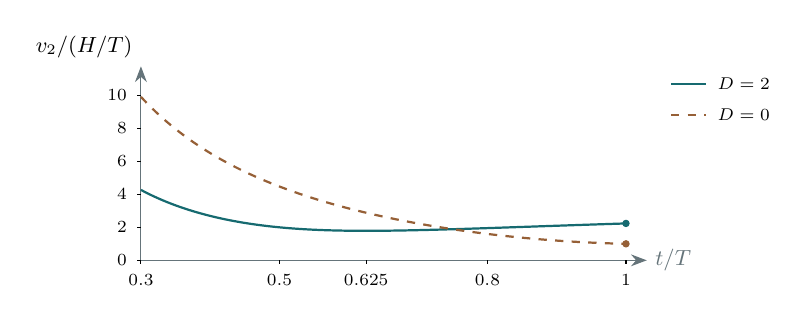
\begin{tikzpicture}[scale=.88,transform shape]
\draw[axis] (0,0.0)--(7.3,0.0) node[right] {$t/T$};
\draw[axis] (0,0)--(0,2.8);
\node[above left] at (0,2.8) {$v_2/(H/T)$};
\draw[thin] (0.000000,0.0)--(0.000000,-0.06);\node[below,font=\scriptsize] at (0.000000,-0.08) {$ 0.3 $};
\draw[thin] (2.000000,0.0)--(2.000000,-0.06);\node[below,font=\scriptsize] at (2.000000,-0.08) {$ 0.5 $};
\draw[thin] (3.250000,0.0)--(3.250000,-0.06);\node[below,font=\scriptsize] at (3.250000,-0.08) {$ 0.625 $};
\draw[thin] (5.000000,0.0)--(5.000000,-0.06);\node[below,font=\scriptsize] at (5.000000,-0.08) {$ 0.8 $};
\draw[thin] (7.000000,0.0)--(7.000000,-0.06);\node[below,font=\scriptsize] at (7.000000,-0.08) {$ 1 $};
\draw[thin] (0,0.000000)--(-.06,0.000000);\node[left,font=\scriptsize] at (-.08,0.000000) {$ 0 $};
\draw[thin] (0,0.476190)--(-.06,0.476190);\node[left,font=\scriptsize] at (-.08,0.476190) {$ 2 $};
\draw[thin] (0,0.952381)--(-.06,0.952381);\node[left,font=\scriptsize] at (-.08,0.952381) {$ 4 $};
\draw[thin] (0,1.428571)--(-.06,1.428571);\node[left,font=\scriptsize] at (-.08,1.428571) {$ 6 $};
\draw[thin] (0,1.904762)--(-.06,1.904762);\node[left,font=\scriptsize] at (-.08,1.904762) {$ 8 $};
\draw[thin] (0,2.380952)--(-.06,2.380952);\node[left,font=\scriptsize] at (-.08,2.380952) {$ 10 $};
\draw[thick,color=accent] plot coordinates {(0.0000000,1.0163689) (0.0291667,1.0008798) (0.0583333,0.9857374) (0.0875000,0.9709329) (0.1166667,0.9564575) (0.1458333,0.9423030) (0.1750000,0.9284615) (0.2041667,0.9149252) (0.2333333,0.9016869) (0.2625000,0.8887394) (0.2916667,0.8760758) (0.3208333,0.8636896) (0.3500000,0.8515745) (0.3791667,0.8397242) (0.4083333,0.8281329) (0.4375000,0.8167949) (0.4666667,0.8057047) (0.4958333,0.7948570) (0.5250000,0.7842466) (0.5541667,0.7738686) (0.5833333,0.7637183) (0.6125000,0.7537909) (0.6416667,0.7440820) (0.6708333,0.7345873) (0.7000000,0.7253026) (0.7291667,0.7162238) (0.7583333,0.7073470) (0.7875000,0.6986684) (0.8166667,0.6901843) (0.8458333,0.6818911) (0.8750000,0.6737853) (0.9041667,0.6658636) (0.9333333,0.6581227) (0.9625000,0.6505594) (0.9916667,0.6431705) (1.0208333,0.6359532) (1.0500000,0.6289044) (1.0791667,0.6220213) (1.1083333,0.6153011) (1.1375000,0.6087411) (1.1666667,0.6023386) (1.1958333,0.5960911) (1.2250000,0.5899960) (1.2541667,0.5840509) (1.2833333,0.5782533) (1.3125000,0.5726009) (1.3416667,0.5670914) (1.3708333,0.5617224) (1.4000000,0.5564918) (1.4291667,0.5513973) (1.4583333,0.5464369) (1.4875000,0.5416083) (1.5166667,0.5369096) (1.5458333,0.5323386) (1.5750000,0.5278934) (1.6041667,0.5235719) (1.6333333,0.5193722) (1.6625000,0.5152924) (1.6916667,0.5113306) (1.7208333,0.5074848) (1.7500000,0.5037532) (1.7791667,0.5001339) (1.8083333,0.4966252) (1.8375000,0.4932252) (1.8666667,0.4899321) (1.8958333,0.4867442) (1.9250000,0.4836596) (1.9541667,0.4806767) (1.9833333,0.4777937) (2.0125000,0.4750089) (2.0416667,0.4723206) (2.0708333,0.4697271) (2.1000000,0.4672267) (2.1291667,0.4648178) (2.1583333,0.4624988) (2.1875000,0.4602678) (2.2166667,0.4581235) (2.2458333,0.4560640) (2.2750000,0.4540879) (2.3041667,0.4521936) (2.3333333,0.4503793) (2.3625000,0.4486437) (2.3916667,0.4469851) (2.4208333,0.4454020) (2.4500000,0.4438929) (2.4791667,0.4424562) (2.5083333,0.4410905) (2.5375000,0.4397942) (2.5666667,0.4385659) (2.5958333,0.4374042) (2.6250000,0.4363075) (2.6541667,0.4352744) (2.6833333,0.4343036) (2.7125000,0.4333936) (2.7416667,0.4325431) (2.7708333,0.4317507) (2.8000000,0.4310149) (2.8291667,0.4303346) (2.8583333,0.4297083) (2.8875000,0.4291349) (2.9166667,0.4286129) (2.9458333,0.4281411) (2.9750000,0.4277184) (3.0041667,0.4273433) (3.0333333,0.4270149) (3.0625000,0.4267317) (3.0916667,0.4264928) (3.1208333,0.4262969) (3.1500000,0.4261429) (3.1791667,0.4260296) (3.2083333,0.4259561) (3.2375000,0.4259211) (3.2666667,0.4259237) (3.2958333,0.4259629) (3.3250000,0.4260375) (3.3541667,0.4261466) (3.3833333,0.4262892) (3.4125000,0.4264644) (3.4416667,0.4266712) (3.4708333,0.4269087) (3.5000000,0.4271760) (3.5291667,0.4274722) (3.5583333,0.4277964) (3.5875000,0.4281478) (3.6166667,0.4285256) (3.6458333,0.4289290) (3.6750000,0.4293571) (3.7041667,0.4298092) (3.7333333,0.4302846) (3.7625000,0.4307824) (3.7916667,0.4313020) (3.8208333,0.4318427) (3.8500000,0.4324038) (3.8791667,0.4329846) (3.9083333,0.4335844) (3.9375000,0.4342027) (3.9666667,0.4348387) (3.9958333,0.4354920) (4.0250000,0.4361618) (4.0541667,0.4368477) (4.0833333,0.4375490) (4.1125000,0.4382652) (4.1416667,0.4389958) (4.1708333,0.4397403) (4.2000000,0.4404980) (4.2291667,0.4412687) (4.2583333,0.4420517) (4.2875000,0.4428466) (4.3166667,0.4436530) (4.3458333,0.4444703) (4.3750000,0.4452983) (4.4041667,0.4461364) (4.4333333,0.4469842) (4.4625000,0.4478414) (4.4916667,0.4487076) (4.5208333,0.4495824) (4.5500000,0.4504654) (4.5791667,0.4513562) (4.6083333,0.4522546) (4.6375000,0.4531602) (4.6666667,0.4540727) (4.6958333,0.4549917) (4.7250000,0.4559170) (4.7541667,0.4568482) (4.7833333,0.4577851) (4.8125000,0.4587274) (4.8416667,0.4596748) (4.8708333,0.4606270) (4.9000000,0.4615838) (4.9291667,0.4625450) (4.9583333,0.4635102) (4.9875000,0.4644794) (5.0166667,0.4654521) (5.0458333,0.4664283) (5.0750000,0.4674076) (5.1041667,0.4683900) (5.1333333,0.4693751) (5.1625000,0.4703628) (5.1916667,0.4713529) (5.2208333,0.4723453) (5.2500000,0.4733397) (5.2791667,0.4743359) (5.3083333,0.4753339) (5.3375000,0.4763333) (5.3666667,0.4773342) (5.3958333,0.4783363) (5.4250000,0.4793395) (5.4541667,0.4803436) (5.4833333,0.4813485) (5.5125000,0.4823540) (5.5416667,0.4833601) (5.5708333,0.4843666) (5.6000000,0.4853734) (5.6291667,0.4863803) (5.6583333,0.4873873) (5.6875000,0.4883942) (5.7166667,0.4894010) (5.7458333,0.4904074) (5.7750000,0.4914135) (5.8041667,0.4924192) (5.8333333,0.4934243) (5.8625000,0.4944287) (5.8916667,0.4954324) (5.9208333,0.4964352) (5.9500000,0.4974372) (5.9791667,0.4984381) (6.0083333,0.4994380) (6.0375000,0.5004368) (6.0666667,0.5014343) (6.0958333,0.5024306) (6.1250000,0.5034255) (6.1541667,0.5044190) (6.1833333,0.5054110) (6.2125000,0.5064015) (6.2416667,0.5073904) (6.2708333,0.5083777) (6.3000000,0.5093632) (6.3291667,0.5103471) (6.3583333,0.5113291) (6.3875000,0.5123092) (6.4166667,0.5132875) (6.4458333,0.5142638) (6.4750000,0.5152381) (6.5041667,0.5162105) (6.5333333,0.5171807) (6.5625000,0.5181489) (6.5916667,0.5191149) (6.6208333,0.5200787) (6.6500000,0.5210403) (6.6791667,0.5219997) (6.7083333,0.5229568) (6.7375000,0.5239117) (6.7666667,0.5248642) (6.7958333,0.5258143) (6.8250000,0.5267620) (6.8541667,0.5277074) (6.8833333,0.5286503) (6.9125000,0.5295907) (6.9416667,0.5305287) (6.9708333,0.5314642) (7.0000000,0.5323971)};
\draw[thick,color=accent] (7.65,2.55)--(8.15,2.55);\node[right,font=\scriptsize] at (8.2,2.55) {$D=2$};
\draw[thick,dashed,color=warm] plot coordinates {(0.0000000,2.3596935) (0.0291667,2.3283391) (0.0583333,2.2975868) (0.0875000,2.2674196) (0.1166667,2.2378211) (0.1458333,2.2087756) (0.1750000,2.1802678) (0.2041667,2.1522832) (0.2333333,2.1248075) (0.2625000,2.0978273) (0.2916667,2.0713293) (0.3208333,2.0453009) (0.3500000,2.0197299) (0.3791667,1.9946046) (0.4083333,1.9699134) (0.4375000,1.9456455) (0.4666667,1.9217901) (0.4958333,1.8983370) (0.5250000,1.8752763) (0.5541667,1.8525983) (0.5833333,1.8302938) (0.6125000,1.8083537) (0.6416667,1.7867694) (0.6708333,1.7655324) (0.7000000,1.7446346) (0.7291667,1.7240680) (0.7583333,1.7038250) (0.7875000,1.6838982) (0.8166667,1.6642804) (0.8458333,1.6449645) (0.8750000,1.6259439) (0.9041667,1.6072120) (0.9333333,1.5887624) (0.9625000,1.5705889) (0.9916667,1.5526855) (1.0208333,1.5350464) (1.0500000,1.5176660) (1.0791667,1.5005388) (1.1083333,1.4836594) (1.1375000,1.4670226) (1.1666667,1.4506234) (1.1958333,1.4344570) (1.2250000,1.4185185) (1.2541667,1.4028033) (1.2833333,1.3873070) (1.3125000,1.3720251) (1.3416667,1.3569534) (1.3708333,1.3420877) (1.4000000,1.3274241) (1.4291667,1.3129585) (1.4583333,1.2986872) (1.4875000,1.2846064) (1.5166667,1.2707125) (1.5458333,1.2570020) (1.5750000,1.2434715) (1.6041667,1.2301175) (1.6333333,1.2169369) (1.6625000,1.2039264) (1.6916667,1.1910829) (1.7208333,1.1784034) (1.7500000,1.1658850) (1.7791667,1.1535248) (1.8083333,1.1413200) (1.8375000,1.1292678) (1.8666667,1.1173656) (1.8958333,1.1056108) (1.9250000,1.0940008) (1.9541667,1.0825331) (1.9833333,1.0712054) (2.0125000,1.0600152) (2.0416667,1.0489603) (2.0708333,1.0380384) (2.1000000,1.0272472) (2.1291667,1.0165848) (2.1583333,1.0060489) (2.1875000,0.9956375) (2.2166667,0.9853487) (2.2458333,0.9751803) (2.2750000,0.9651306) (2.3041667,0.9551977) (2.3333333,0.9453798) (2.3625000,0.9356750) (2.3916667,0.9260816) (2.4208333,0.9165979) (2.4500000,0.9072223) (2.4791667,0.8979531) (2.5083333,0.8887888) (2.5375000,0.8797277) (2.5666667,0.8707683) (2.5958333,0.8619092) (2.6250000,0.8531490) (2.6541667,0.8444861) (2.6833333,0.8359192) (2.7125000,0.8274469) (2.7416667,0.8190679) (2.7708333,0.8107808) (2.8000000,0.8025845) (2.8291667,0.7944777) (2.8583333,0.7864591) (2.8875000,0.7785275) (2.9166667,0.7706818) (2.9458333,0.7629209) (2.9750000,0.7552435) (3.0041667,0.7476487) (3.0333333,0.7401353) (3.0625000,0.7327023) (3.0916667,0.7253487) (3.1208333,0.7180735) (3.1500000,0.7108756) (3.1791667,0.7037542) (3.2083333,0.6967082) (3.2375000,0.6897368) (3.2666667,0.6828391) (3.2958333,0.6760141) (3.3250000,0.6692611) (3.3541667,0.6625791) (3.3833333,0.6559674) (3.4125000,0.6494251) (3.4416667,0.6429514) (3.4708333,0.6365456) (3.5000000,0.6302070) (3.5291667,0.6239347) (3.5583333,0.6177281) (3.5875000,0.6115864) (3.6166667,0.6055090) (3.6458333,0.5994951) (3.6750000,0.5935442) (3.7041667,0.5876556) (3.7333333,0.5818285) (3.7625000,0.5760626) (3.7916667,0.5703570) (3.8208333,0.5647112) (3.8500000,0.5591247) (3.8791667,0.5535969) (3.9083333,0.5481273) (3.9375000,0.5427152) (3.9666667,0.5373602) (3.9958333,0.5320618) (4.0250000,0.5268195) (4.0541667,0.5216327) (4.0833333,0.5165011) (4.1125000,0.5114241) (4.1416667,0.5064013) (4.1708333,0.5014322) (4.2000000,0.4965165) (4.2291667,0.4916537) (4.2583333,0.4868434) (4.2875000,0.4820852) (4.3166667,0.4773787) (4.3458333,0.4727236) (4.3750000,0.4681195) (4.4041667,0.4635659) (4.4333333,0.4590627) (4.4625000,0.4546094) (4.4916667,0.4502058) (4.5208333,0.4458515) (4.5500000,0.4415462) (4.5791667,0.4372895) (4.6083333,0.4330814) (4.6375000,0.4289213) (4.6666667,0.4248092) (4.6958333,0.4207447) (4.7250000,0.4167275) (4.7541667,0.4127575) (4.7833333,0.4088344) (4.8125000,0.4049579) (4.8416667,0.4011279) (4.8708333,0.3973442) (4.9000000,0.3936065) (4.9291667,0.3899146) (4.9583333,0.3862684) (4.9875000,0.3826676) (5.0166667,0.3791122) (5.0458333,0.3756019) (5.0750000,0.3721366) (5.1041667,0.3687162) (5.1333333,0.3653404) (5.1625000,0.3620092) (5.1916667,0.3587224) (5.2208333,0.3554799) (5.2500000,0.3522815) (5.2791667,0.3491273) (5.3083333,0.3460169) (5.3375000,0.3429504) (5.3666667,0.3399277) (5.3958333,0.3369486) (5.4250000,0.3340131) (5.4541667,0.3311210) (5.4833333,0.3282723) (5.5125000,0.3254670) (5.5416667,0.3227049) (5.5708333,0.3199859) (5.6000000,0.3173101) (5.6291667,0.3146772) (5.6583333,0.3120874) (5.6875000,0.3095404) (5.7166667,0.3070364) (5.7458333,0.3045751) (5.7750000,0.3021565) (5.8041667,0.2997806) (5.8333333,0.2974474) (5.8625000,0.2951567) (5.8916667,0.2929085) (5.9208333,0.2907028) (5.9500000,0.2885394) (5.9791667,0.2864185) (6.0083333,0.2843398) (6.0375000,0.2823033) (6.0666667,0.2803089) (6.0958333,0.2783567) (6.1250000,0.2764464) (6.1541667,0.2745782) (6.1833333,0.2727517) (6.2125000,0.2709671) (6.2416667,0.2692241) (6.2708333,0.2675227) (6.3000000,0.2658629) (6.3291667,0.2642444) (6.3583333,0.2626672) (6.3875000,0.2611312) (6.4166667,0.2596363) (6.4458333,0.2581822) (6.4750000,0.2567690) (6.5041667,0.2553963) (6.5333333,0.2540642) (6.5625000,0.2527724) (6.5916667,0.2515207) (6.6208333,0.2503090) (6.6500000,0.2491370) (6.6791667,0.2480047) (6.7083333,0.2469117) (6.7375000,0.2458579) (6.7666667,0.2448430) (6.7958333,0.2438668) (6.8250000,0.2429291) (6.8541667,0.2420296) (6.8833333,0.2411680) (6.9125000,0.2403440) (6.9416667,0.2395575) (6.9708333,0.2388080) (7.0000000,0.2380952)};
\draw[thick,dashed,color=warm] (7.65,2.0999999999999996)--(8.15,2.0999999999999996);\node[right,font=\scriptsize] at (8.2,2.0999999999999996) {$D=0$};
\draw[fill=white,color=accent] (7.0000000,0.5323971) circle(.045);\draw[fill=white,color=warm] (7,0.2380952) circle(.045);
\end{tikzpicture}
\figcaption{解图力试1.1B\quad 时间曲线比较可取极小值与末时刻极限}
\end{minipage}\end{center}
速度平面给出同一求导过程的几何解释。令$s=1/t$，
\[
(u_x,u_y)=(v_1,0)+s(-a,H),\qquad s>1/T.
\]
速度端点从$s=1/T$的空心点$U_T$沿$(-a,H)$方向伸展。由速度原点到整条直线作垂线，垂足$U_*$给整条直线的最短距离。解图力试1.1C左侧的$U_*$位于允许射线内，对应$t_*<T$；右侧的垂足位于射线端点之前，最短可行速度只能趋向端点。
\begin{center}\begin{minipage}{.98\linewidth}\centering
\begin{tikzpicture}[scale=.7,transform shape]
\begin{scope}[shift={(0,0)}]
\draw[axis] (-2.7,0)--(4.7,0) node[right] {$u_x$};\draw[axis] (0,0)--(0,2.2) node[above] {$u_y$};
\draw[guide] (4,0)--(2,1);
\draw[thick,color=accent] plot coordinates {(2.0000000,1.0000000) (1.9900000,1.0050000) (1.9800000,1.0100000) (1.9700000,1.0150000) (1.9600000,1.0200000) (1.9500000,1.0250000) (1.9400000,1.0300000) (1.9300000,1.0350000) (1.9200000,1.0400000) (1.9100000,1.0450000) (1.9000000,1.0500000) (1.8900000,1.0550000) (1.8800000,1.0600000) (1.8700000,1.0650000) (1.8600000,1.0700000) (1.8500000,1.0750000) (1.8400000,1.0800000) (1.8300000,1.0850000) (1.8200000,1.0900000) (1.8100000,1.0950000) (1.8000000,1.1000000) (1.7900000,1.1050000) (1.7800000,1.1100000) (1.7700000,1.1150000) (1.7600000,1.1200000) (1.7500000,1.1250000) (1.7400000,1.1300000) (1.7300000,1.1350000) (1.7200000,1.1400000) (1.7100000,1.1450000) (1.7000000,1.1500000) (1.6900000,1.1550000) (1.6800000,1.1600000) (1.6700000,1.1650000) (1.6600000,1.1700000) (1.6500000,1.1750000) (1.6400000,1.1800000) (1.6300000,1.1850000) (1.6200000,1.1900000) (1.6100000,1.1950000) (1.6000000,1.2000000) (1.5900000,1.2050000) (1.5800000,1.2100000) (1.5700000,1.2150000) (1.5600000,1.2200000) (1.5500000,1.2250000) (1.5400000,1.2300000) (1.5300000,1.2350000) (1.5200000,1.2400000) (1.5100000,1.2450000) (1.5000000,1.2500000) (1.4900000,1.2550000) (1.4800000,1.2600000) (1.4700000,1.2650000) (1.4600000,1.2700000) (1.4500000,1.2750000) (1.4400000,1.2800000) (1.4300000,1.2850000) (1.4200000,1.2900000) (1.4100000,1.2950000) (1.4000000,1.3000000) (1.3900000,1.3050000) (1.3800000,1.3100000) (1.3700000,1.3150000) (1.3600000,1.3200000) (1.3500000,1.3250000) (1.3400000,1.3300000) (1.3300000,1.3350000) (1.3200000,1.3400000) (1.3100000,1.3450000) (1.3000000,1.3500000) (1.2900000,1.3550000) (1.2800000,1.3600000) (1.2700000,1.3650000) (1.2600000,1.3700000) (1.2500000,1.3750000) (1.2400000,1.3800000) (1.2300000,1.3850000) (1.2200000,1.3900000) (1.2100000,1.3950000) (1.2000000,1.4000000) (1.1900000,1.4050000) (1.1800000,1.4100000) (1.1700000,1.4150000) (1.1600000,1.4200000) (1.1500000,1.4250000) (1.1400000,1.4300000) (1.1300000,1.4350000) (1.1200000,1.4400000) (1.1100000,1.4450000) (1.1000000,1.4500000) (1.0900000,1.4550000) (1.0800000,1.4600000) (1.0700000,1.4650000) (1.0600000,1.4700000) (1.0500000,1.4750000) (1.0400000,1.4800000) (1.0300000,1.4850000) (1.0200000,1.4900000) (1.0100000,1.4950000) (1.0000000,1.5000000) (0.9900000,1.5050000) (0.9800000,1.5100000) (0.9700000,1.5150000) (0.9600000,1.5200000) (0.9500000,1.5250000) (0.9400000,1.5300000) (0.9300000,1.5350000) (0.9200000,1.5400000) (0.9100000,1.5450000) (0.9000000,1.5500000) (0.8900000,1.5550000) (0.8800000,1.5600000) (0.8700000,1.5650000) (0.8600000,1.5700000) (0.8500000,1.5750000) (0.8400000,1.5800000) (0.8300000,1.5850000) (0.8200000,1.5900000) (0.8100000,1.5950000) (0.8000000,1.6000000)};
\draw[fill=white] (2,1) circle(.06) node[below right] {$U_T$};
\fill[color=warm] (0.8000000,1.6000000) circle(.045);
\draw[guide] (0,0)--(0.8000000,1.6000000);
\node[above] at (1,2.6) {内点最优：$D=2$};
\node[above right] at (.8,1.6) {$U_*$};
\draw[motion] (.9,1.55)--(.55,1.725);
\end{scope}
\begin{scope}[shift={(8.5,0)}]
\draw[axis] (-2.7,0)--(4.7,0) node[right] {$u_x$};\draw[axis] (0,0)--(0,2.2) node[above] {$u_y$};
\draw[guide] (4,0)--(0,1);
\draw[thick,color=accent] plot coordinates {(0.0000000,1.0000000) (-0.0200000,1.0050000) (-0.0400000,1.0100000) (-0.0600000,1.0150000) (-0.0800000,1.0200000) (-0.1000000,1.0250000) (-0.1200000,1.0300000) (-0.1400000,1.0350000) (-0.1600000,1.0400000) (-0.1800000,1.0450000) (-0.2000000,1.0500000) (-0.2200000,1.0550000) (-0.2400000,1.0600000) (-0.2600000,1.0650000) (-0.2800000,1.0700000) (-0.3000000,1.0750000) (-0.3200000,1.0800000) (-0.3400000,1.0850000) (-0.3600000,1.0900000) (-0.3800000,1.0950000) (-0.4000000,1.1000000) (-0.4200000,1.1050000) (-0.4400000,1.1100000) (-0.4600000,1.1150000) (-0.4800000,1.1200000) (-0.5000000,1.1250000) (-0.5200000,1.1300000) (-0.5400000,1.1350000) (-0.5600000,1.1400000) (-0.5800000,1.1450000) (-0.6000000,1.1500000) (-0.6200000,1.1550000) (-0.6400000,1.1600000) (-0.6600000,1.1650000) (-0.6800000,1.1700000) (-0.7000000,1.1750000) (-0.7200000,1.1800000) (-0.7400000,1.1850000) (-0.7600000,1.1900000) (-0.7800000,1.1950000) (-0.8000000,1.2000000) (-0.8200000,1.2050000) (-0.8400000,1.2100000) (-0.8600000,1.2150000) (-0.8800000,1.2200000) (-0.9000000,1.2250000) (-0.9200000,1.2300000) (-0.9400000,1.2350000) (-0.9600000,1.2400000) (-0.9800000,1.2450000) (-1.0000000,1.2500000) (-1.0200000,1.2550000) (-1.0400000,1.2600000) (-1.0600000,1.2650000) (-1.0800000,1.2700000) (-1.1000000,1.2750000) (-1.1200000,1.2800000) (-1.1400000,1.2850000) (-1.1600000,1.2900000) (-1.1800000,1.2950000) (-1.2000000,1.3000000) (-1.2200000,1.3050000) (-1.2400000,1.3100000) (-1.2600000,1.3150000) (-1.2800000,1.3200000) (-1.3000000,1.3250000) (-1.3200000,1.3300000) (-1.3400000,1.3350000) (-1.3600000,1.3400000) (-1.3800000,1.3450000) (-1.4000000,1.3500000) (-1.4200000,1.3550000) (-1.4400000,1.3600000) (-1.4600000,1.3650000) (-1.4800000,1.3700000) (-1.5000000,1.3750000) (-1.5200000,1.3800000) (-1.5400000,1.3850000) (-1.5600000,1.3900000) (-1.5800000,1.3950000) (-1.6000000,1.4000000) (-1.6200000,1.4050000) (-1.6400000,1.4100000) (-1.6600000,1.4150000) (-1.6800000,1.4200000) (-1.7000000,1.4250000) (-1.7200000,1.4300000) (-1.7400000,1.4350000) (-1.7600000,1.4400000) (-1.7800000,1.4450000) (-1.8000000,1.4500000) (-1.8200000,1.4550000) (-1.8400000,1.4600000) (-1.8600000,1.4650000) (-1.8800000,1.4700000) (-1.9000000,1.4750000) (-1.9200000,1.4800000) (-1.9400000,1.4850000) (-1.9600000,1.4900000) (-1.9800000,1.4950000) (-2.0000000,1.5000000) (-2.0200000,1.5050000) (-2.0400000,1.5100000) (-2.0600000,1.5150000) (-2.0800000,1.5200000) (-2.1000000,1.5250000) (-2.1200000,1.5300000) (-2.1400000,1.5350000) (-2.1600000,1.5400000) (-2.1800000,1.5450000) (-2.2000000,1.5500000) (-2.2200000,1.5550000) (-2.2400000,1.5600000) (-2.2600000,1.5650000) (-2.2800000,1.5700000) (-2.3000000,1.5750000) (-2.3200000,1.5800000) (-2.3400000,1.5850000) (-2.3600000,1.5900000) (-2.3800000,1.5950000) (-2.4000000,1.6000000)};
\draw[fill=white] (0,1) circle(.06) node[below right] {$U_T$};
\fill[color=warm] (0.2352941,0.9411765) circle(.045);
\draw[guide] (0,0)--(0.2352941,0.9411765);
\node[above] at (1,2.6) {末时刻极限：$D=0$};
\draw[guide] (.2352941,.9411765)--(1.2,1.9);\node[above right] at (1.2,1.9) {$U_*$};
\draw[motion] (-2.0,1.5)--(-2.6,1.65);
\end{scope}
\end{tikzpicture}
\figcaption{解图力试1.1C\quad 实线为允许速度射线，空心点为t等于T的极限，U星为整条直线垂足}
\end{minipage}\end{center}
若$D(L-D)\le H^2$，包括$a\le0$及$t_*=T$，则在$0<t<T$中速度持续下降，其下确界为
\[
\inf_{0<t<T}v_2
=\sqrt{F(T)}
=\boxed{\frac{\sqrt{D^2+H^2}}{T}}.
\]
飞行中拦截所需速度严格大于此下界，它在$t\to T^-$时被任意逼近。若将落地瞬间也计入相遇，定义域改为$0<t\le T$，同一数值便在$t=T$取到。两类结果由时间区间的开、闭端点决定。

在可取的内点极小值处，把$t_*$代回两个初速分量，得到
\[
u_{x*}=\frac{v_1H^2}{a^2+H^2},\qquad
u_{y*}=\frac{v_1aH}{a^2+H^2},
\quad
\boxed{\alpha_*=\arctan\frac{L-D}{H}}.
\]
此时$a>0$且$u_{x*},u_{y*}>0$，发射角在第一象限。在其余情形，初速端点趋向$U_T=(D/T,H/T)$，因而极限方向为
\[
\alpha\longrightarrow\operatorname{atan2}(H,D)
\quad(t\to T^-).
\]
例如$D=0$时，炮位就在目标处，极限发射为竖直向上，速度趋向$H/T=\sqrt{gH/2}$；任一$t<T$所需速度更大。两问的方向条件由对应时刻的分量式直接给出。

解图力试1.1D进一步把可取内点最优的位置写成$D$的区间。二次函数$D(L-D)$在$D=L/2$最大，最大值为$L^2/4$。因此存在这种炮位的条件是$L>2H$，即$v_1>\sqrt{2gH}$；两临界位置为
\[
 D_\pm=\frac{L\pm\sqrt{L^2-4H^2}}2,\qquad D_-<D<D_+.
\]
在两个端点处$t_*=T$，仍是末时刻极限。图中的抛物线与水平线$H^2$的交点将可取极小值和仅有下确界的炮位分开，与前面的时间及速度图一致。
\begin{center}\begin{minipage}{.98\linewidth}\centering
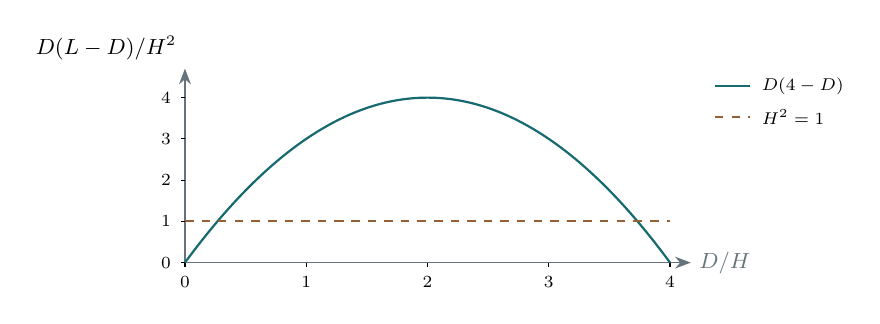
\begin{tikzpicture}[scale=.88,transform shape]
\draw[axis] (0,0.0)--(7.3,0.0) node[right] {$D/H$};
\draw[axis] (0,0)--(0,2.8);
\node[above left] at (0,2.8) {$D(L-D)/H^2$};
\draw[thin] (0.000000,0.0)--(0.000000,-0.06);\node[below,font=\scriptsize] at (0.000000,-0.08) {$ 0 $};
\draw[thin] (1.750000,0.0)--(1.750000,-0.06);\node[below,font=\scriptsize] at (1.750000,-0.08) {$ 1 $};
\draw[thin] (3.500000,0.0)--(3.500000,-0.06);\node[below,font=\scriptsize] at (3.500000,-0.08) {$ 2 $};
\draw[thin] (5.250000,0.0)--(5.250000,-0.06);\node[below,font=\scriptsize] at (5.250000,-0.08) {$ 3 $};
\draw[thin] (7.000000,0.0)--(7.000000,-0.06);\node[below,font=\scriptsize] at (7.000000,-0.08) {$ 4 $};
\draw[thin] (0,0.000000)--(-.06,0.000000);\node[left,font=\scriptsize] at (-.08,0.000000) {$ 0 $};
\draw[thin] (0,0.595238)--(-.06,0.595238);\node[left,font=\scriptsize] at (-.08,0.595238) {$ 1 $};
\draw[thin] (0,1.190476)--(-.06,1.190476);\node[left,font=\scriptsize] at (-.08,1.190476) {$ 2 $};
\draw[thin] (0,1.785714)--(-.06,1.785714);\node[left,font=\scriptsize] at (-.08,1.785714) {$ 3 $};
\draw[thin] (0,2.380952)--(-.06,2.380952);\node[left,font=\scriptsize] at (-.08,2.380952) {$ 4 $};
\draw[thick,color=accent] plot coordinates {(0.0000000,0.0000000) (0.0291667,0.0395172) (0.0583333,0.0787037) (0.0875000,0.1175595) (0.1166667,0.1560847) (0.1458333,0.1942791) (0.1750000,0.2321429) (0.2041667,0.2696759) (0.2333333,0.3068783) (0.2625000,0.3437500) (0.2916667,0.3802910) (0.3208333,0.4165013) (0.3500000,0.4523810) (0.3791667,0.4879299) (0.4083333,0.5231481) (0.4375000,0.5580357) (0.4666667,0.5925926) (0.4958333,0.6268188) (0.5250000,0.6607143) (0.5541667,0.6942791) (0.5833333,0.7275132) (0.6125000,0.7604167) (0.6416667,0.7929894) (0.6708333,0.8252315) (0.7000000,0.8571429) (0.7291667,0.8887235) (0.7583333,0.9199735) (0.7875000,0.9508929) (0.8166667,0.9814815) (0.8458333,1.0117394) (0.8750000,1.0416667) (0.9041667,1.0712632) (0.9333333,1.1005291) (0.9625000,1.1294643) (0.9916667,1.1580688) (1.0208333,1.1863426) (1.0500000,1.2142857) (1.0791667,1.2418981) (1.1083333,1.2691799) (1.1375000,1.2961310) (1.1666667,1.3227513) (1.1958333,1.3490410) (1.2250000,1.3750000) (1.2541667,1.4006283) (1.2833333,1.4259259) (1.3125000,1.4508929) (1.3416667,1.4755291) (1.3708333,1.4998347) (1.4000000,1.5238095) (1.4291667,1.5474537) (1.4583333,1.5707672) (1.4875000,1.5937500) (1.5166667,1.6164021) (1.5458333,1.6387235) (1.5750000,1.6607143) (1.6041667,1.6823743) (1.6333333,1.7037037) (1.6625000,1.7247024) (1.6916667,1.7453704) (1.7208333,1.7657077) (1.7500000,1.7857143) (1.7791667,1.8053902) (1.8083333,1.8247354) (1.8375000,1.8437500) (1.8666667,1.8624339) (1.8958333,1.8807870) (1.9250000,1.8988095) (1.9541667,1.9165013) (1.9833333,1.9338624) (2.0125000,1.9508929) (2.0416667,1.9675926) (2.0708333,1.9839616) (2.1000000,2.0000000) (2.1291667,2.0157077) (2.1583333,2.0310847) (2.1875000,2.0461310) (2.2166667,2.0608466) (2.2458333,2.0752315) (2.2750000,2.0892857) (2.3041667,2.1030093) (2.3333333,2.1164021) (2.3625000,2.1294643) (2.3916667,2.1421958) (2.4208333,2.1545966) (2.4500000,2.1666667) (2.4791667,2.1784061) (2.5083333,2.1898148) (2.5375000,2.2008929) (2.5666667,2.2116402) (2.5958333,2.2220569) (2.6250000,2.2321429) (2.6541667,2.2418981) (2.6833333,2.2513228) (2.7125000,2.2604167) (2.7416667,2.2691799) (2.7708333,2.2776124) (2.8000000,2.2857143) (2.8291667,2.2934854) (2.8583333,2.3009259) (2.8875000,2.3080357) (2.9166667,2.3148148) (2.9458333,2.3212632) (2.9750000,2.3273810) (3.0041667,2.3331680) (3.0333333,2.3386243) (3.0625000,2.3437500) (3.0916667,2.3485450) (3.1208333,2.3530093) (3.1500000,2.3571429) (3.1791667,2.3609458) (3.2083333,2.3644180) (3.2375000,2.3675595) (3.2666667,2.3703704) (3.2958333,2.3728505) (3.3250000,2.3750000) (3.3541667,2.3768188) (3.3833333,2.3783069) (3.4125000,2.3794643) (3.4416667,2.3802910) (3.4708333,2.3807870) (3.5000000,2.3809524) (3.5291667,2.3807870) (3.5583333,2.3802910) (3.5875000,2.3794643) (3.6166667,2.3783069) (3.6458333,2.3768188) (3.6750000,2.3750000) (3.7041667,2.3728505) (3.7333333,2.3703704) (3.7625000,2.3675595) (3.7916667,2.3644180) (3.8208333,2.3609458) (3.8500000,2.3571429) (3.8791667,2.3530093) (3.9083333,2.3485450) (3.9375000,2.3437500) (3.9666667,2.3386243) (3.9958333,2.3331680) (4.0250000,2.3273810) (4.0541667,2.3212632) (4.0833333,2.3148148) (4.1125000,2.3080357) (4.1416667,2.3009259) (4.1708333,2.2934854) (4.2000000,2.2857143) (4.2291667,2.2776124) (4.2583333,2.2691799) (4.2875000,2.2604167) (4.3166667,2.2513228) (4.3458333,2.2418981) (4.3750000,2.2321429) (4.4041667,2.2220569) (4.4333333,2.2116402) (4.4625000,2.2008929) (4.4916667,2.1898148) (4.5208333,2.1784061) (4.5500000,2.1666667) (4.5791667,2.1545966) (4.6083333,2.1421958) (4.6375000,2.1294643) (4.6666667,2.1164021) (4.6958333,2.1030093) (4.7250000,2.0892857) (4.7541667,2.0752315) (4.7833333,2.0608466) (4.8125000,2.0461310) (4.8416667,2.0310847) (4.8708333,2.0157077) (4.9000000,2.0000000) (4.9291667,1.9839616) (4.9583333,1.9675926) (4.9875000,1.9508929) (5.0166667,1.9338624) (5.0458333,1.9165013) (5.0750000,1.8988095) (5.1041667,1.8807870) (5.1333333,1.8624339) (5.1625000,1.8437500) (5.1916667,1.8247354) (5.2208333,1.8053902) (5.2500000,1.7857143) (5.2791667,1.7657077) (5.3083333,1.7453704) (5.3375000,1.7247024) (5.3666667,1.7037037) (5.3958333,1.6823743) (5.4250000,1.6607143) (5.4541667,1.6387235) (5.4833333,1.6164021) (5.5125000,1.5937500) (5.5416667,1.5707672) (5.5708333,1.5474537) (5.6000000,1.5238095) (5.6291667,1.4998347) (5.6583333,1.4755291) (5.6875000,1.4508929) (5.7166667,1.4259259) (5.7458333,1.4006283) (5.7750000,1.3750000) (5.8041667,1.3490410) (5.8333333,1.3227513) (5.8625000,1.2961310) (5.8916667,1.2691799) (5.9208333,1.2418981) (5.9500000,1.2142857) (5.9791667,1.1863426) (6.0083333,1.1580688) (6.0375000,1.1294643) (6.0666667,1.1005291) (6.0958333,1.0712632) (6.1250000,1.0416667) (6.1541667,1.0117394) (6.1833333,0.9814815) (6.2125000,0.9508929) (6.2416667,0.9199735) (6.2708333,0.8887235) (6.3000000,0.8571429) (6.3291667,0.8252315) (6.3583333,0.7929894) (6.3875000,0.7604167) (6.4166667,0.7275132) (6.4458333,0.6942791) (6.4750000,0.6607143) (6.5041667,0.6268188) (6.5333333,0.5925926) (6.5625000,0.5580357) (6.5916667,0.5231481) (6.6208333,0.4879299) (6.6500000,0.4523810) (6.6791667,0.4165013) (6.7083333,0.3802910) (6.7375000,0.3437500) (6.7666667,0.3068783) (6.7958333,0.2696759) (6.8250000,0.2321429) (6.8541667,0.1942791) (6.8833333,0.1560847) (6.9125000,0.1175595) (6.9416667,0.0787037) (6.9708333,0.0395172) (7.0000000,0.0000000)};
\draw[thick,color=accent] (7.65,2.55)--(8.15,2.55);\node[right,font=\scriptsize] at (8.2,2.55) {$D(4-D)$};
\draw[thick,dashed,color=warm] plot coordinates {(0.0000000,0.5952381) (0.0291667,0.5952381) (0.0583333,0.5952381) (0.0875000,0.5952381) (0.1166667,0.5952381) (0.1458333,0.5952381) (0.1750000,0.5952381) (0.2041667,0.5952381) (0.2333333,0.5952381) (0.2625000,0.5952381) (0.2916667,0.5952381) (0.3208333,0.5952381) (0.3500000,0.5952381) (0.3791667,0.5952381) (0.4083333,0.5952381) (0.4375000,0.5952381) (0.4666667,0.5952381) (0.4958333,0.5952381) (0.5250000,0.5952381) (0.5541667,0.5952381) (0.5833333,0.5952381) (0.6125000,0.5952381) (0.6416667,0.5952381) (0.6708333,0.5952381) (0.7000000,0.5952381) (0.7291667,0.5952381) (0.7583333,0.5952381) (0.7875000,0.5952381) (0.8166667,0.5952381) (0.8458333,0.5952381) (0.8750000,0.5952381) (0.9041667,0.5952381) (0.9333333,0.5952381) (0.9625000,0.5952381) (0.9916667,0.5952381) (1.0208333,0.5952381) (1.0500000,0.5952381) (1.0791667,0.5952381) (1.1083333,0.5952381) (1.1375000,0.5952381) (1.1666667,0.5952381) (1.1958333,0.5952381) (1.2250000,0.5952381) (1.2541667,0.5952381) (1.2833333,0.5952381) (1.3125000,0.5952381) (1.3416667,0.5952381) (1.3708333,0.5952381) (1.4000000,0.5952381) (1.4291667,0.5952381) (1.4583333,0.5952381) (1.4875000,0.5952381) (1.5166667,0.5952381) (1.5458333,0.5952381) (1.5750000,0.5952381) (1.6041667,0.5952381) (1.6333333,0.5952381) (1.6625000,0.5952381) (1.6916667,0.5952381) (1.7208333,0.5952381) (1.7500000,0.5952381) (1.7791667,0.5952381) (1.8083333,0.5952381) (1.8375000,0.5952381) (1.8666667,0.5952381) (1.8958333,0.5952381) (1.9250000,0.5952381) (1.9541667,0.5952381) (1.9833333,0.5952381) (2.0125000,0.5952381) (2.0416667,0.5952381) (2.0708333,0.5952381) (2.1000000,0.5952381) (2.1291667,0.5952381) (2.1583333,0.5952381) (2.1875000,0.5952381) (2.2166667,0.5952381) (2.2458333,0.5952381) (2.2750000,0.5952381) (2.3041667,0.5952381) (2.3333333,0.5952381) (2.3625000,0.5952381) (2.3916667,0.5952381) (2.4208333,0.5952381) (2.4500000,0.5952381) (2.4791667,0.5952381) (2.5083333,0.5952381) (2.5375000,0.5952381) (2.5666667,0.5952381) (2.5958333,0.5952381) (2.6250000,0.5952381) (2.6541667,0.5952381) (2.6833333,0.5952381) (2.7125000,0.5952381) (2.7416667,0.5952381) (2.7708333,0.5952381) (2.8000000,0.5952381) (2.8291667,0.5952381) (2.8583333,0.5952381) (2.8875000,0.5952381) (2.9166667,0.5952381) (2.9458333,0.5952381) (2.9750000,0.5952381) (3.0041667,0.5952381) (3.0333333,0.5952381) (3.0625000,0.5952381) (3.0916667,0.5952381) (3.1208333,0.5952381) (3.1500000,0.5952381) (3.1791667,0.5952381) (3.2083333,0.5952381) (3.2375000,0.5952381) (3.2666667,0.5952381) (3.2958333,0.5952381) (3.3250000,0.5952381) (3.3541667,0.5952381) (3.3833333,0.5952381) (3.4125000,0.5952381) (3.4416667,0.5952381) (3.4708333,0.5952381) (3.5000000,0.5952381) (3.5291667,0.5952381) (3.5583333,0.5952381) (3.5875000,0.5952381) (3.6166667,0.5952381) (3.6458333,0.5952381) (3.6750000,0.5952381) (3.7041667,0.5952381) (3.7333333,0.5952381) (3.7625000,0.5952381) (3.7916667,0.5952381) (3.8208333,0.5952381) (3.8500000,0.5952381) (3.8791667,0.5952381) (3.9083333,0.5952381) (3.9375000,0.5952381) (3.9666667,0.5952381) (3.9958333,0.5952381) (4.0250000,0.5952381) (4.0541667,0.5952381) (4.0833333,0.5952381) (4.1125000,0.5952381) (4.1416667,0.5952381) (4.1708333,0.5952381) (4.2000000,0.5952381) (4.2291667,0.5952381) (4.2583333,0.5952381) (4.2875000,0.5952381) (4.3166667,0.5952381) (4.3458333,0.5952381) (4.3750000,0.5952381) (4.4041667,0.5952381) (4.4333333,0.5952381) (4.4625000,0.5952381) (4.4916667,0.5952381) (4.5208333,0.5952381) (4.5500000,0.5952381) (4.5791667,0.5952381) (4.6083333,0.5952381) (4.6375000,0.5952381) (4.6666667,0.5952381) (4.6958333,0.5952381) (4.7250000,0.5952381) (4.7541667,0.5952381) (4.7833333,0.5952381) (4.8125000,0.5952381) (4.8416667,0.5952381) (4.8708333,0.5952381) (4.9000000,0.5952381) (4.9291667,0.5952381) (4.9583333,0.5952381) (4.9875000,0.5952381) (5.0166667,0.5952381) (5.0458333,0.5952381) (5.0750000,0.5952381) (5.1041667,0.5952381) (5.1333333,0.5952381) (5.1625000,0.5952381) (5.1916667,0.5952381) (5.2208333,0.5952381) (5.2500000,0.5952381) (5.2791667,0.5952381) (5.3083333,0.5952381) (5.3375000,0.5952381) (5.3666667,0.5952381) (5.3958333,0.5952381) (5.4250000,0.5952381) (5.4541667,0.5952381) (5.4833333,0.5952381) (5.5125000,0.5952381) (5.5416667,0.5952381) (5.5708333,0.5952381) (5.6000000,0.5952381) (5.6291667,0.5952381) (5.6583333,0.5952381) (5.6875000,0.5952381) (5.7166667,0.5952381) (5.7458333,0.5952381) (5.7750000,0.5952381) (5.8041667,0.5952381) (5.8333333,0.5952381) (5.8625000,0.5952381) (5.8916667,0.5952381) (5.9208333,0.5952381) (5.9500000,0.5952381) (5.9791667,0.5952381) (6.0083333,0.5952381) (6.0375000,0.5952381) (6.0666667,0.5952381) (6.0958333,0.5952381) (6.1250000,0.5952381) (6.1541667,0.5952381) (6.1833333,0.5952381) (6.2125000,0.5952381) (6.2416667,0.5952381) (6.2708333,0.5952381) (6.3000000,0.5952381) (6.3291667,0.5952381) (6.3583333,0.5952381) (6.3875000,0.5952381) (6.4166667,0.5952381) (6.4458333,0.5952381) (6.4750000,0.5952381) (6.5041667,0.5952381) (6.5333333,0.5952381) (6.5625000,0.5952381) (6.5916667,0.5952381) (6.6208333,0.5952381) (6.6500000,0.5952381) (6.6791667,0.5952381) (6.7083333,0.5952381) (6.7375000,0.5952381) (6.7666667,0.5952381) (6.7958333,0.5952381) (6.8250000,0.5952381) (6.8541667,0.5952381) (6.8833333,0.5952381) (6.9125000,0.5952381) (6.9416667,0.5952381) (6.9708333,0.5952381) (7.0000000,0.5952381)};
\draw[thick,dashed,color=warm] (7.65,2.0999999999999996)--(8.15,2.0999999999999996);\node[right,font=\scriptsize] at (8.2,2.0999999999999996) {$H^2=1$};
\end{tikzpicture}
\figcaption{解图力试1.1D\quad 抛物线高于水平线的炮位给落地前内点最优}
\end{minipage}\end{center}


\Needspace{8\baselineskip}

\pdfbookmark[3]{关键洞察}{q1-h5}

\subsection*{关键洞察}

共同重力使相对运动为匀速直线，同时通过落地时间限制可用的相对运动段。速度平面上的整条直线、允许射线和端点分别对应无约束垂距、飞行中方案及落地时方案，最小速度是否可取由这三个位置决定。

\Needspace{8\baselineskip}

\pdfbookmark[3]{易错点}{q1-h6}

\subsection*{易错点}

\begin{itemize}
\item 两弹同时发射，相遇式中的时间相同；先求$T$再限定$t$。
\item $a=L-D$可以取负，炮位在投弹点左侧时仍按同一坐标式求解。
\item 角度式平方后产生候选根，回代未平方关系及$0<t<T$选出实际发射状态。
\item $D(L-D)=H^2$给$t_*=T$，与严格落地前的内点最优分开。
\item 下确界由$t\to T^-$逼近，包含落地瞬间的闭区间才允许端点取等。\end{itemize}

\Needspace{8\baselineskip}

\pdfbookmark[3]{课堂讲解建议}{q1-h7}

\subsection*{课堂讲解建议}

先在A图让学生逐项相减两弹坐标，说明重力项消去而$g$仍通过$T$限制时间。再把同一$t$同时标在B图和C图，定位垂足对应的实际高度。比较$D/H=2$与$D/H=0$两个归一化算例，逐步算出$t_*$、碰撞高度和速度端点。最后用D图求可取内点最优的炮位范围，并将角度二次式的实根与允许射线中的点对应。

\Needspace{8\baselineskip}

\pdfbookmark[3]{变式训练}{q1-h8}

\subsection*{变式训练}

\begin{enumerate}
\item \textbf{可取的内点最小值。}取$H=1,g=2,v_1=4,D=2$，求最小发射速度、方向与碰撞位置。

$T=1,L=4,a=2$，故$t_*=(2^2+1)/(4\times2)=5/8<1$。回代得
\[
 u_{x*}=4/5,\quad u_{y*}=8/5,\quad
 v_{2,\min}=4/\sqrt5,\quad \alpha_*=\arctan2.
\]
碰撞点为$x_C=4(5/8)=5/2$，$y_C=1-(5/8)^2=39/64>0$。变图力试1.1V1画所需速度与相遇时间，极小点在允许时间内，两个分量还给$\tan\alpha_*=2$。
\begin{center}\begin{minipage}{.98\linewidth}\centering
\begin{tikzpicture}[scale=.88,transform shape]
\draw[axis] (0,0.0)--(7.3,0.0) node[right] {$t/T$};
\draw[axis] (0,0)--(0,2.8);
\node[above left] at (0,2.8) {$v_2/(H/T)$};
\draw[thin] (0.000000,0.0)--(0.000000,-0.06);\node[below,font=\scriptsize] at (0.000000,-0.08) {$ 0.3 $};
\draw[thin] (2.000000,0.0)--(2.000000,-0.06);\node[below,font=\scriptsize] at (2.000000,-0.08) {$ 0.5 $};
\draw[thin] (3.250000,0.0)--(3.250000,-0.06);\node[below,font=\scriptsize] at (3.250000,-0.08) {$ 0.625 $};
\draw[thin] (5.000000,0.0)--(5.000000,-0.06);\node[below,font=\scriptsize] at (5.000000,-0.08) {$ 0.8 $};
\draw[thin] (7.000000,0.0)--(7.000000,-0.06);\node[below,font=\scriptsize] at (7.000000,-0.08) {$ 1 $};
\draw[thin] (0,0.000000)--(-.06,0.000000);\node[left,font=\scriptsize] at (-.08,0.000000) {$ 0 $};
\draw[thin] (0,0.500000)--(-.06,0.500000);\node[left,font=\scriptsize] at (-.08,0.500000) {$ 1 $};
\draw[thin] (0,1.000000)--(-.06,1.000000);\node[left,font=\scriptsize] at (-.08,1.000000) {$ 2 $};
\draw[thin] (0,1.500000)--(-.06,1.500000);\node[left,font=\scriptsize] at (-.08,1.500000) {$ 3 $};
\draw[thin] (0,2.000000)--(-.06,2.000000);\node[left,font=\scriptsize] at (-.08,2.000000) {$ 4 $};
\draw[thin] (0,2.500000)--(-.06,2.500000);\node[left,font=\scriptsize] at (-.08,2.500000) {$ 5 $};
\draw[thick,color=accent] plot coordinates {(0.0000000,2.1343747) (0.0291667,2.1018476) (0.0583333,2.0700486) (0.0875000,2.0389590) (0.1166667,2.0085607) (0.1458333,1.9788363) (0.1750000,1.9497691) (0.2041667,1.9213430) (0.2333333,1.8935425) (0.2625000,1.8663527) (0.2916667,1.8397592) (0.3208333,1.8137482) (0.3500000,1.7883064) (0.3791667,1.7634208) (0.4083333,1.7390791) (0.4375000,1.7152693) (0.4666667,1.6919799) (0.4958333,1.6691996) (0.5250000,1.6469179) (0.5541667,1.6251241) (0.5833333,1.6038083) (0.6125000,1.5829608) (0.6416667,1.5625722) (0.6708333,1.5426333) (0.7000000,1.5231354) (0.7291667,1.5040700) (0.7583333,1.4854287) (0.7875000,1.4672037) (0.8166667,1.4493870) (0.8458333,1.4319713) (0.8750000,1.4149492) (0.9041667,1.3983136) (0.9333333,1.3820576) (0.9625000,1.3661746) (0.9916667,1.3506581) (1.0208333,1.3355017) (1.0500000,1.3206992) (1.0791667,1.3062447) (1.1083333,1.2921322) (1.1375000,1.2783562) (1.1666667,1.2649111) (1.1958333,1.2517913) (1.2250000,1.2389917) (1.2541667,1.2265069) (1.2833333,1.2143320) (1.3125000,1.2024619) (1.3416667,1.1908919) (1.3708333,1.1796170) (1.4000000,1.1686327) (1.4291667,1.1579344) (1.4583333,1.1475174) (1.4875000,1.1373774) (1.5166667,1.1275101) (1.5458333,1.1179110) (1.5750000,1.1085760) (1.6041667,1.0995010) (1.6333333,1.0906816) (1.6625000,1.0821141) (1.6916667,1.0737942) (1.7208333,1.0657180) (1.7500000,1.0578816) (1.7791667,1.0502812) (1.8083333,1.0429129) (1.8375000,1.0357729) (1.8666667,1.0288574) (1.8958333,1.0221627) (1.9250000,1.0156852) (1.9541667,1.0094211) (1.9833333,1.0033668) (2.0125000,0.9975187) (2.0416667,0.9918733) (2.0708333,0.9864269) (2.1000000,0.9811762) (2.1291667,0.9761175) (2.1583333,0.9712474) (2.1875000,0.9665625) (2.2166667,0.9620593) (2.2458333,0.9577345) (2.2750000,0.9535847) (2.3041667,0.9496065) (2.3333333,0.9457966) (2.3625000,0.9421518) (2.3916667,0.9386688) (2.4208333,0.9353443) (2.4500000,0.9321751) (2.4791667,0.9291581) (2.5083333,0.9262900) (2.5375000,0.9235679) (2.5666667,0.9209885) (2.5958333,0.9185487) (2.6250000,0.9162457) (2.6541667,0.9140763) (2.6833333,0.9120376) (2.7125000,0.9101266) (2.7416667,0.9083405) (2.7708333,0.9066764) (2.8000000,0.9051314) (2.8291667,0.9037027) (2.8583333,0.9023875) (2.8875000,0.9011832) (2.9166667,0.9000871) (2.9458333,0.8990964) (2.9750000,0.8982085) (3.0041667,0.8974210) (3.0333333,0.8967312) (3.0625000,0.8961367) (3.0916667,0.8956349) (3.1208333,0.8952235) (3.1500000,0.8949000) (3.1791667,0.8946622) (3.2083333,0.8945078) (3.2375000,0.8944344) (3.2666667,0.8944398) (3.2958333,0.8945220) (3.3250000,0.8946787) (3.3541667,0.8949078) (3.3833333,0.8952073) (3.4125000,0.8955752) (3.4416667,0.8960095) (3.4708333,0.8965082) (3.5000000,0.8970695) (3.5291667,0.8976915) (3.5583333,0.8983724) (3.5875000,0.8991104) (3.6166667,0.8999038) (3.6458333,0.9007508) (3.6750000,0.9016499) (3.7041667,0.9025993) (3.7333333,0.9035976) (3.7625000,0.9046431) (3.7916667,0.9057343) (3.8208333,0.9068697) (3.8500000,0.9080480) (3.8791667,0.9092676) (3.9083333,0.9105273) (3.9375000,0.9118257) (3.9666667,0.9131614) (3.9958333,0.9145332) (4.0250000,0.9159398) (4.0541667,0.9173801) (4.0833333,0.9188529) (4.1125000,0.9203570) (4.1416667,0.9218912) (4.1708333,0.9234545) (4.2000000,0.9250459) (4.2291667,0.9266642) (4.2583333,0.9283085) (4.2875000,0.9299779) (4.3166667,0.9316712) (4.3458333,0.9333877) (4.3750000,0.9351264) (4.4041667,0.9368864) (4.4333333,0.9386669) (4.4625000,0.9404670) (4.4916667,0.9422860) (4.5208333,0.9441230) (4.5500000,0.9459773) (4.5791667,0.9478481) (4.6083333,0.9497348) (4.6375000,0.9516365) (4.6666667,0.9535527) (4.6958333,0.9554827) (4.7250000,0.9574257) (4.7541667,0.9593813) (4.7833333,0.9613488) (4.8125000,0.9633276) (4.8416667,0.9653171) (4.8708333,0.9673167) (4.9000000,0.9693261) (4.9291667,0.9713445) (4.9583333,0.9733715) (4.9875000,0.9754066) (5.0166667,0.9774494) (5.0458333,0.9794993) (5.0750000,0.9815560) (5.1041667,0.9836189) (5.1333333,0.9856877) (5.1625000,0.9877619) (5.1916667,0.9898412) (5.2208333,0.9919251) (5.2500000,0.9940133) (5.2791667,0.9961054) (5.3083333,0.9982011) (5.3375000,1.0003000) (5.3666667,1.0024018) (5.3958333,1.0045062) (5.4250000,1.0066129) (5.4541667,1.0087215) (5.4833333,1.0108318) (5.5125000,1.0129434) (5.5416667,1.0150562) (5.5708333,1.0171698) (5.6000000,1.0192840) (5.6291667,1.0213986) (5.6583333,1.0235133) (5.6875000,1.0256278) (5.7166667,1.0277420) (5.7458333,1.0298556) (5.7750000,1.0319685) (5.8041667,1.0340803) (5.8333333,1.0361910) (5.8625000,1.0383002) (5.8916667,1.0404080) (5.9208333,1.0425140) (5.9500000,1.0446180) (5.9791667,1.0467201) (6.0083333,1.0488198) (6.0375000,1.0509172) (6.0666667,1.0530120) (6.0958333,1.0551042) (6.1250000,1.0571935) (6.1541667,1.0592799) (6.1833333,1.0613631) (6.2125000,1.0634432) (6.2416667,1.0655199) (6.2708333,1.0675931) (6.3000000,1.0696628) (6.3291667,1.0717288) (6.3583333,1.0737910) (6.3875000,1.0758494) (6.4166667,1.0779037) (6.4458333,1.0799540) (6.4750000,1.0820001) (6.5041667,1.0840420) (6.5333333,1.0860795) (6.5625000,1.0881126) (6.5916667,1.0901412) (6.6208333,1.0921653) (6.6500000,1.0941847) (6.6791667,1.0961994) (6.7083333,1.0982094) (6.7375000,1.1002145) (6.7666667,1.1022147) (6.7958333,1.1042100) (6.8250000,1.1062003) (6.8541667,1.1081855) (6.8833333,1.1101656) (6.9125000,1.1121405) (6.9416667,1.1141103) (6.9708333,1.1160748) (7.0000000,1.1180340)};
\draw[fill=white,color=accent] (7.0000000,1.1180340) circle(.045);
\end{tikzpicture}
\figcaption{变图力试1.1V1\quad D等于2时的可取最小发射速度}
\end{minipage}\end{center}
\item \textbf{炮位就在目标处。}保持$H=1,g=2,v_1=4$，改为$D=0$，求飞行中拦截的速度下界。

此时$a=4$，无约束驻点$t_*=17/16$在落地时刻之后。允许区间中$F(t)$下降，$u_x=4-4/t$、$u_y=1/t$，所以$\inf v_2=1$，方向趋向竖直向上。变图力试1.1V2的末端为空心点。取$t=0.9$便有$u_x=-4/9,u_y=10/9$、$v_2=\sqrt{116}/9>1$，相遇高度0.19，给出实际飞行中的逼近方案。
\begin{center}\begin{minipage}{.98\linewidth}\centering
\begin{tikzpicture}[scale=.88,transform shape]
\draw[axis] (0,0.0)--(7.3,0.0) node[right] {$t/T$};
\draw[axis] (0,0)--(0,2.8);
\node[above left] at (0,2.8) {$v_2/(H/T)$};
\draw[thin] (0.000000,0.0)--(0.000000,-0.06);\node[below,font=\scriptsize] at (0.000000,-0.08) {$ 0.3 $};
\draw[thin] (2.000000,0.0)--(2.000000,-0.06);\node[below,font=\scriptsize] at (2.000000,-0.08) {$ 0.5 $};
\draw[thin] (4.500000,0.0)--(4.500000,-0.06);\node[below,font=\scriptsize] at (4.500000,-0.08) {$ 0.75 $};
\draw[thin] (7.000000,0.0)--(7.000000,-0.06);\node[below,font=\scriptsize] at (7.000000,-0.08) {$ 1 $};
\draw[thin] (0,0.000000)--(-.06,0.000000);\node[left,font=\scriptsize] at (-.08,0.000000) {$ 0 $};
\draw[thin] (0,0.476190)--(-.06,0.476190);\node[left,font=\scriptsize] at (-.08,0.476190) {$ 2 $};
\draw[thin] (0,0.952381)--(-.06,0.952381);\node[left,font=\scriptsize] at (-.08,0.952381) {$ 4 $};
\draw[thin] (0,1.428571)--(-.06,1.428571);\node[left,font=\scriptsize] at (-.08,1.428571) {$ 6 $};
\draw[thin] (0,1.904762)--(-.06,1.904762);\node[left,font=\scriptsize] at (-.08,1.904762) {$ 8 $};
\draw[thin] (0,2.380952)--(-.06,2.380952);\node[left,font=\scriptsize] at (-.08,2.380952) {$ 10 $};
\draw[thick,color=accent] plot coordinates {(0.0000000,2.3596935) (0.0291667,2.3283391) (0.0583333,2.2975868) (0.0875000,2.2674196) (0.1166667,2.2378211) (0.1458333,2.2087756) (0.1750000,2.1802678) (0.2041667,2.1522832) (0.2333333,2.1248075) (0.2625000,2.0978273) (0.2916667,2.0713293) (0.3208333,2.0453009) (0.3500000,2.0197299) (0.3791667,1.9946046) (0.4083333,1.9699134) (0.4375000,1.9456455) (0.4666667,1.9217901) (0.4958333,1.8983370) (0.5250000,1.8752763) (0.5541667,1.8525983) (0.5833333,1.8302938) (0.6125000,1.8083537) (0.6416667,1.7867694) (0.6708333,1.7655324) (0.7000000,1.7446346) (0.7291667,1.7240680) (0.7583333,1.7038250) (0.7875000,1.6838982) (0.8166667,1.6642804) (0.8458333,1.6449645) (0.8750000,1.6259439) (0.9041667,1.6072120) (0.9333333,1.5887624) (0.9625000,1.5705889) (0.9916667,1.5526855) (1.0208333,1.5350464) (1.0500000,1.5176660) (1.0791667,1.5005388) (1.1083333,1.4836594) (1.1375000,1.4670226) (1.1666667,1.4506234) (1.1958333,1.4344570) (1.2250000,1.4185185) (1.2541667,1.4028033) (1.2833333,1.3873070) (1.3125000,1.3720251) (1.3416667,1.3569534) (1.3708333,1.3420877) (1.4000000,1.3274241) (1.4291667,1.3129585) (1.4583333,1.2986872) (1.4875000,1.2846064) (1.5166667,1.2707125) (1.5458333,1.2570020) (1.5750000,1.2434715) (1.6041667,1.2301175) (1.6333333,1.2169369) (1.6625000,1.2039264) (1.6916667,1.1910829) (1.7208333,1.1784034) (1.7500000,1.1658850) (1.7791667,1.1535248) (1.8083333,1.1413200) (1.8375000,1.1292678) (1.8666667,1.1173656) (1.8958333,1.1056108) (1.9250000,1.0940008) (1.9541667,1.0825331) (1.9833333,1.0712054) (2.0125000,1.0600152) (2.0416667,1.0489603) (2.0708333,1.0380384) (2.1000000,1.0272472) (2.1291667,1.0165848) (2.1583333,1.0060489) (2.1875000,0.9956375) (2.2166667,0.9853487) (2.2458333,0.9751803) (2.2750000,0.9651306) (2.3041667,0.9551977) (2.3333333,0.9453798) (2.3625000,0.9356750) (2.3916667,0.9260816) (2.4208333,0.9165979) (2.4500000,0.9072223) (2.4791667,0.8979531) (2.5083333,0.8887888) (2.5375000,0.8797277) (2.5666667,0.8707683) (2.5958333,0.8619092) (2.6250000,0.8531490) (2.6541667,0.8444861) (2.6833333,0.8359192) (2.7125000,0.8274469) (2.7416667,0.8190679) (2.7708333,0.8107808) (2.8000000,0.8025845) (2.8291667,0.7944777) (2.8583333,0.7864591) (2.8875000,0.7785275) (2.9166667,0.7706818) (2.9458333,0.7629209) (2.9750000,0.7552435) (3.0041667,0.7476487) (3.0333333,0.7401353) (3.0625000,0.7327023) (3.0916667,0.7253487) (3.1208333,0.7180735) (3.1500000,0.7108756) (3.1791667,0.7037542) (3.2083333,0.6967082) (3.2375000,0.6897368) (3.2666667,0.6828391) (3.2958333,0.6760141) (3.3250000,0.6692611) (3.3541667,0.6625791) (3.3833333,0.6559674) (3.4125000,0.6494251) (3.4416667,0.6429514) (3.4708333,0.6365456) (3.5000000,0.6302070) (3.5291667,0.6239347) (3.5583333,0.6177281) (3.5875000,0.6115864) (3.6166667,0.6055090) (3.6458333,0.5994951) (3.6750000,0.5935442) (3.7041667,0.5876556) (3.7333333,0.5818285) (3.7625000,0.5760626) (3.7916667,0.5703570) (3.8208333,0.5647112) (3.8500000,0.5591247) (3.8791667,0.5535969) (3.9083333,0.5481273) (3.9375000,0.5427152) (3.9666667,0.5373602) (3.9958333,0.5320618) (4.0250000,0.5268195) (4.0541667,0.5216327) (4.0833333,0.5165011) (4.1125000,0.5114241) (4.1416667,0.5064013) (4.1708333,0.5014322) (4.2000000,0.4965165) (4.2291667,0.4916537) (4.2583333,0.4868434) (4.2875000,0.4820852) (4.3166667,0.4773787) (4.3458333,0.4727236) (4.3750000,0.4681195) (4.4041667,0.4635659) (4.4333333,0.4590627) (4.4625000,0.4546094) (4.4916667,0.4502058) (4.5208333,0.4458515) (4.5500000,0.4415462) (4.5791667,0.4372895) (4.6083333,0.4330814) (4.6375000,0.4289213) (4.6666667,0.4248092) (4.6958333,0.4207447) (4.7250000,0.4167275) (4.7541667,0.4127575) (4.7833333,0.4088344) (4.8125000,0.4049579) (4.8416667,0.4011279) (4.8708333,0.3973442) (4.9000000,0.3936065) (4.9291667,0.3899146) (4.9583333,0.3862684) (4.9875000,0.3826676) (5.0166667,0.3791122) (5.0458333,0.3756019) (5.0750000,0.3721366) (5.1041667,0.3687162) (5.1333333,0.3653404) (5.1625000,0.3620092) (5.1916667,0.3587224) (5.2208333,0.3554799) (5.2500000,0.3522815) (5.2791667,0.3491273) (5.3083333,0.3460169) (5.3375000,0.3429504) (5.3666667,0.3399277) (5.3958333,0.3369486) (5.4250000,0.3340131) (5.4541667,0.3311210) (5.4833333,0.3282723) (5.5125000,0.3254670) (5.5416667,0.3227049) (5.5708333,0.3199859) (5.6000000,0.3173101) (5.6291667,0.3146772) (5.6583333,0.3120874) (5.6875000,0.3095404) (5.7166667,0.3070364) (5.7458333,0.3045751) (5.7750000,0.3021565) (5.8041667,0.2997806) (5.8333333,0.2974474) (5.8625000,0.2951567) (5.8916667,0.2929085) (5.9208333,0.2907028) (5.9500000,0.2885394) (5.9791667,0.2864185) (6.0083333,0.2843398) (6.0375000,0.2823033) (6.0666667,0.2803089) (6.0958333,0.2783567) (6.1250000,0.2764464) (6.1541667,0.2745782) (6.1833333,0.2727517) (6.2125000,0.2709671) (6.2416667,0.2692241) (6.2708333,0.2675227) (6.3000000,0.2658629) (6.3291667,0.2642444) (6.3583333,0.2626672) (6.3875000,0.2611312) (6.4166667,0.2596363) (6.4458333,0.2581822) (6.4750000,0.2567690) (6.5041667,0.2553963) (6.5333333,0.2540642) (6.5625000,0.2527724) (6.5916667,0.2515207) (6.6208333,0.2503090) (6.6500000,0.2491370) (6.6791667,0.2480047) (6.7083333,0.2469117) (6.7375000,0.2458579) (6.7666667,0.2448430) (6.7958333,0.2438668) (6.8250000,0.2429291) (6.8541667,0.2420296) (6.8833333,0.2411680) (6.9125000,0.2403440) (6.9416667,0.2395575) (6.9708333,0.2388080) (7.0000000,0.2380952)};
\draw[fill=white,color=accent] (7.0000000,0.2380952) circle(.045);
\end{tikzpicture}
\figcaption{变图力试1.1V2\quad D等于0时速度向1下降，末时刻端点为空心}
\end{minipage}\end{center}
\item \textbf{可取最小值的炮位区间。}给定$H,g,v_1$，求存在内点最优的必要充分条件和全部炮位。

$D(L-D)>H^2$要求开口向下的二次函数超过$H^2$。其最大值为$L^2/4$，所以条件为$L>2H$，等价于$v_1>\sqrt{2gH}$。解二次方程得
\[
 \frac{L-\sqrt{L^2-4H^2}}2<D<
 \frac{L+\sqrt{L^2-4H^2}}2.
\]
变图力试1.1V3取$L/H=4$，两端为$D/H=2\pm\sqrt3$，中间位置对应$t_*<T$；端点的碰撞恰在地面。
\begin{center}\begin{minipage}{.98\linewidth}\centering
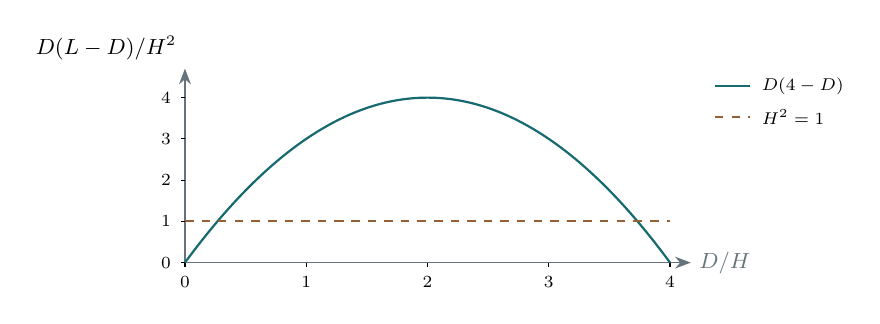
\begin{tikzpicture}[scale=.88,transform shape]
\draw[axis] (0,0.0)--(7.3,0.0) node[right] {$D/H$};
\draw[axis] (0,0)--(0,2.8);
\node[above left] at (0,2.8) {$D(L-D)/H^2$};
\draw[thin] (0.000000,0.0)--(0.000000,-0.06);\node[below,font=\scriptsize] at (0.000000,-0.08) {$ 0 $};
\draw[thin] (1.750000,0.0)--(1.750000,-0.06);\node[below,font=\scriptsize] at (1.750000,-0.08) {$ 1 $};
\draw[thin] (3.500000,0.0)--(3.500000,-0.06);\node[below,font=\scriptsize] at (3.500000,-0.08) {$ 2 $};
\draw[thin] (5.250000,0.0)--(5.250000,-0.06);\node[below,font=\scriptsize] at (5.250000,-0.08) {$ 3 $};
\draw[thin] (7.000000,0.0)--(7.000000,-0.06);\node[below,font=\scriptsize] at (7.000000,-0.08) {$ 4 $};
\draw[thin] (0,0.000000)--(-.06,0.000000);\node[left,font=\scriptsize] at (-.08,0.000000) {$ 0 $};
\draw[thin] (0,0.595238)--(-.06,0.595238);\node[left,font=\scriptsize] at (-.08,0.595238) {$ 1 $};
\draw[thin] (0,1.190476)--(-.06,1.190476);\node[left,font=\scriptsize] at (-.08,1.190476) {$ 2 $};
\draw[thin] (0,1.785714)--(-.06,1.785714);\node[left,font=\scriptsize] at (-.08,1.785714) {$ 3 $};
\draw[thin] (0,2.380952)--(-.06,2.380952);\node[left,font=\scriptsize] at (-.08,2.380952) {$ 4 $};
\draw[thick,color=accent] plot coordinates {(0.0000000,0.0000000) (0.0291667,0.0395172) (0.0583333,0.0787037) (0.0875000,0.1175595) (0.1166667,0.1560847) (0.1458333,0.1942791) (0.1750000,0.2321429) (0.2041667,0.2696759) (0.2333333,0.3068783) (0.2625000,0.3437500) (0.2916667,0.3802910) (0.3208333,0.4165013) (0.3500000,0.4523810) (0.3791667,0.4879299) (0.4083333,0.5231481) (0.4375000,0.5580357) (0.4666667,0.5925926) (0.4958333,0.6268188) (0.5250000,0.6607143) (0.5541667,0.6942791) (0.5833333,0.7275132) (0.6125000,0.7604167) (0.6416667,0.7929894) (0.6708333,0.8252315) (0.7000000,0.8571429) (0.7291667,0.8887235) (0.7583333,0.9199735) (0.7875000,0.9508929) (0.8166667,0.9814815) (0.8458333,1.0117394) (0.8750000,1.0416667) (0.9041667,1.0712632) (0.9333333,1.1005291) (0.9625000,1.1294643) (0.9916667,1.1580688) (1.0208333,1.1863426) (1.0500000,1.2142857) (1.0791667,1.2418981) (1.1083333,1.2691799) (1.1375000,1.2961310) (1.1666667,1.3227513) (1.1958333,1.3490410) (1.2250000,1.3750000) (1.2541667,1.4006283) (1.2833333,1.4259259) (1.3125000,1.4508929) (1.3416667,1.4755291) (1.3708333,1.4998347) (1.4000000,1.5238095) (1.4291667,1.5474537) (1.4583333,1.5707672) (1.4875000,1.5937500) (1.5166667,1.6164021) (1.5458333,1.6387235) (1.5750000,1.6607143) (1.6041667,1.6823743) (1.6333333,1.7037037) (1.6625000,1.7247024) (1.6916667,1.7453704) (1.7208333,1.7657077) (1.7500000,1.7857143) (1.7791667,1.8053902) (1.8083333,1.8247354) (1.8375000,1.8437500) (1.8666667,1.8624339) (1.8958333,1.8807870) (1.9250000,1.8988095) (1.9541667,1.9165013) (1.9833333,1.9338624) (2.0125000,1.9508929) (2.0416667,1.9675926) (2.0708333,1.9839616) (2.1000000,2.0000000) (2.1291667,2.0157077) (2.1583333,2.0310847) (2.1875000,2.0461310) (2.2166667,2.0608466) (2.2458333,2.0752315) (2.2750000,2.0892857) (2.3041667,2.1030093) (2.3333333,2.1164021) (2.3625000,2.1294643) (2.3916667,2.1421958) (2.4208333,2.1545966) (2.4500000,2.1666667) (2.4791667,2.1784061) (2.5083333,2.1898148) (2.5375000,2.2008929) (2.5666667,2.2116402) (2.5958333,2.2220569) (2.6250000,2.2321429) (2.6541667,2.2418981) (2.6833333,2.2513228) (2.7125000,2.2604167) (2.7416667,2.2691799) (2.7708333,2.2776124) (2.8000000,2.2857143) (2.8291667,2.2934854) (2.8583333,2.3009259) (2.8875000,2.3080357) (2.9166667,2.3148148) (2.9458333,2.3212632) (2.9750000,2.3273810) (3.0041667,2.3331680) (3.0333333,2.3386243) (3.0625000,2.3437500) (3.0916667,2.3485450) (3.1208333,2.3530093) (3.1500000,2.3571429) (3.1791667,2.3609458) (3.2083333,2.3644180) (3.2375000,2.3675595) (3.2666667,2.3703704) (3.2958333,2.3728505) (3.3250000,2.3750000) (3.3541667,2.3768188) (3.3833333,2.3783069) (3.4125000,2.3794643) (3.4416667,2.3802910) (3.4708333,2.3807870) (3.5000000,2.3809524) (3.5291667,2.3807870) (3.5583333,2.3802910) (3.5875000,2.3794643) (3.6166667,2.3783069) (3.6458333,2.3768188) (3.6750000,2.3750000) (3.7041667,2.3728505) (3.7333333,2.3703704) (3.7625000,2.3675595) (3.7916667,2.3644180) (3.8208333,2.3609458) (3.8500000,2.3571429) (3.8791667,2.3530093) (3.9083333,2.3485450) (3.9375000,2.3437500) (3.9666667,2.3386243) (3.9958333,2.3331680) (4.0250000,2.3273810) (4.0541667,2.3212632) (4.0833333,2.3148148) (4.1125000,2.3080357) (4.1416667,2.3009259) (4.1708333,2.2934854) (4.2000000,2.2857143) (4.2291667,2.2776124) (4.2583333,2.2691799) (4.2875000,2.2604167) (4.3166667,2.2513228) (4.3458333,2.2418981) (4.3750000,2.2321429) (4.4041667,2.2220569) (4.4333333,2.2116402) (4.4625000,2.2008929) (4.4916667,2.1898148) (4.5208333,2.1784061) (4.5500000,2.1666667) (4.5791667,2.1545966) (4.6083333,2.1421958) (4.6375000,2.1294643) (4.6666667,2.1164021) (4.6958333,2.1030093) (4.7250000,2.0892857) (4.7541667,2.0752315) (4.7833333,2.0608466) (4.8125000,2.0461310) (4.8416667,2.0310847) (4.8708333,2.0157077) (4.9000000,2.0000000) (4.9291667,1.9839616) (4.9583333,1.9675926) (4.9875000,1.9508929) (5.0166667,1.9338624) (5.0458333,1.9165013) (5.0750000,1.8988095) (5.1041667,1.8807870) (5.1333333,1.8624339) (5.1625000,1.8437500) (5.1916667,1.8247354) (5.2208333,1.8053902) (5.2500000,1.7857143) (5.2791667,1.7657077) (5.3083333,1.7453704) (5.3375000,1.7247024) (5.3666667,1.7037037) (5.3958333,1.6823743) (5.4250000,1.6607143) (5.4541667,1.6387235) (5.4833333,1.6164021) (5.5125000,1.5937500) (5.5416667,1.5707672) (5.5708333,1.5474537) (5.6000000,1.5238095) (5.6291667,1.4998347) (5.6583333,1.4755291) (5.6875000,1.4508929) (5.7166667,1.4259259) (5.7458333,1.4006283) (5.7750000,1.3750000) (5.8041667,1.3490410) (5.8333333,1.3227513) (5.8625000,1.2961310) (5.8916667,1.2691799) (5.9208333,1.2418981) (5.9500000,1.2142857) (5.9791667,1.1863426) (6.0083333,1.1580688) (6.0375000,1.1294643) (6.0666667,1.1005291) (6.0958333,1.0712632) (6.1250000,1.0416667) (6.1541667,1.0117394) (6.1833333,0.9814815) (6.2125000,0.9508929) (6.2416667,0.9199735) (6.2708333,0.8887235) (6.3000000,0.8571429) (6.3291667,0.8252315) (6.3583333,0.7929894) (6.3875000,0.7604167) (6.4166667,0.7275132) (6.4458333,0.6942791) (6.4750000,0.6607143) (6.5041667,0.6268188) (6.5333333,0.5925926) (6.5625000,0.5580357) (6.5916667,0.5231481) (6.6208333,0.4879299) (6.6500000,0.4523810) (6.6791667,0.4165013) (6.7083333,0.3802910) (6.7375000,0.3437500) (6.7666667,0.3068783) (6.7958333,0.2696759) (6.8250000,0.2321429) (6.8541667,0.1942791) (6.8833333,0.1560847) (6.9125000,0.1175595) (6.9416667,0.0787037) (6.9708333,0.0395172) (7.0000000,0.0000000)};
\draw[thick,color=accent] (7.65,2.55)--(8.15,2.55);\node[right,font=\scriptsize] at (8.2,2.55) {$D(4-D)$};
\draw[thick,dashed,color=warm] plot coordinates {(0.0000000,0.5952381) (0.0291667,0.5952381) (0.0583333,0.5952381) (0.0875000,0.5952381) (0.1166667,0.5952381) (0.1458333,0.5952381) (0.1750000,0.5952381) (0.2041667,0.5952381) (0.2333333,0.5952381) (0.2625000,0.5952381) (0.2916667,0.5952381) (0.3208333,0.5952381) (0.3500000,0.5952381) (0.3791667,0.5952381) (0.4083333,0.5952381) (0.4375000,0.5952381) (0.4666667,0.5952381) (0.4958333,0.5952381) (0.5250000,0.5952381) (0.5541667,0.5952381) (0.5833333,0.5952381) (0.6125000,0.5952381) (0.6416667,0.5952381) (0.6708333,0.5952381) (0.7000000,0.5952381) (0.7291667,0.5952381) (0.7583333,0.5952381) (0.7875000,0.5952381) (0.8166667,0.5952381) (0.8458333,0.5952381) (0.8750000,0.5952381) (0.9041667,0.5952381) (0.9333333,0.5952381) (0.9625000,0.5952381) (0.9916667,0.5952381) (1.0208333,0.5952381) (1.0500000,0.5952381) (1.0791667,0.5952381) (1.1083333,0.5952381) (1.1375000,0.5952381) (1.1666667,0.5952381) (1.1958333,0.5952381) (1.2250000,0.5952381) (1.2541667,0.5952381) (1.2833333,0.5952381) (1.3125000,0.5952381) (1.3416667,0.5952381) (1.3708333,0.5952381) (1.4000000,0.5952381) (1.4291667,0.5952381) (1.4583333,0.5952381) (1.4875000,0.5952381) (1.5166667,0.5952381) (1.5458333,0.5952381) (1.5750000,0.5952381) (1.6041667,0.5952381) (1.6333333,0.5952381) (1.6625000,0.5952381) (1.6916667,0.5952381) (1.7208333,0.5952381) (1.7500000,0.5952381) (1.7791667,0.5952381) (1.8083333,0.5952381) (1.8375000,0.5952381) (1.8666667,0.5952381) (1.8958333,0.5952381) (1.9250000,0.5952381) (1.9541667,0.5952381) (1.9833333,0.5952381) (2.0125000,0.5952381) (2.0416667,0.5952381) (2.0708333,0.5952381) (2.1000000,0.5952381) (2.1291667,0.5952381) (2.1583333,0.5952381) (2.1875000,0.5952381) (2.2166667,0.5952381) (2.2458333,0.5952381) (2.2750000,0.5952381) (2.3041667,0.5952381) (2.3333333,0.5952381) (2.3625000,0.5952381) (2.3916667,0.5952381) (2.4208333,0.5952381) (2.4500000,0.5952381) (2.4791667,0.5952381) (2.5083333,0.5952381) (2.5375000,0.5952381) (2.5666667,0.5952381) (2.5958333,0.5952381) (2.6250000,0.5952381) (2.6541667,0.5952381) (2.6833333,0.5952381) (2.7125000,0.5952381) (2.7416667,0.5952381) (2.7708333,0.5952381) (2.8000000,0.5952381) (2.8291667,0.5952381) (2.8583333,0.5952381) (2.8875000,0.5952381) (2.9166667,0.5952381) (2.9458333,0.5952381) (2.9750000,0.5952381) (3.0041667,0.5952381) (3.0333333,0.5952381) (3.0625000,0.5952381) (3.0916667,0.5952381) (3.1208333,0.5952381) (3.1500000,0.5952381) (3.1791667,0.5952381) (3.2083333,0.5952381) (3.2375000,0.5952381) (3.2666667,0.5952381) (3.2958333,0.5952381) (3.3250000,0.5952381) (3.3541667,0.5952381) (3.3833333,0.5952381) (3.4125000,0.5952381) (3.4416667,0.5952381) (3.4708333,0.5952381) (3.5000000,0.5952381) (3.5291667,0.5952381) (3.5583333,0.5952381) (3.5875000,0.5952381) (3.6166667,0.5952381) (3.6458333,0.5952381) (3.6750000,0.5952381) (3.7041667,0.5952381) (3.7333333,0.5952381) (3.7625000,0.5952381) (3.7916667,0.5952381) (3.8208333,0.5952381) (3.8500000,0.5952381) (3.8791667,0.5952381) (3.9083333,0.5952381) (3.9375000,0.5952381) (3.9666667,0.5952381) (3.9958333,0.5952381) (4.0250000,0.5952381) (4.0541667,0.5952381) (4.0833333,0.5952381) (4.1125000,0.5952381) (4.1416667,0.5952381) (4.1708333,0.5952381) (4.2000000,0.5952381) (4.2291667,0.5952381) (4.2583333,0.5952381) (4.2875000,0.5952381) (4.3166667,0.5952381) (4.3458333,0.5952381) (4.3750000,0.5952381) (4.4041667,0.5952381) (4.4333333,0.5952381) (4.4625000,0.5952381) (4.4916667,0.5952381) (4.5208333,0.5952381) (4.5500000,0.5952381) (4.5791667,0.5952381) (4.6083333,0.5952381) (4.6375000,0.5952381) (4.6666667,0.5952381) (4.6958333,0.5952381) (4.7250000,0.5952381) (4.7541667,0.5952381) (4.7833333,0.5952381) (4.8125000,0.5952381) (4.8416667,0.5952381) (4.8708333,0.5952381) (4.9000000,0.5952381) (4.9291667,0.5952381) (4.9583333,0.5952381) (4.9875000,0.5952381) (5.0166667,0.5952381) (5.0458333,0.5952381) (5.0750000,0.5952381) (5.1041667,0.5952381) (5.1333333,0.5952381) (5.1625000,0.5952381) (5.1916667,0.5952381) (5.2208333,0.5952381) (5.2500000,0.5952381) (5.2791667,0.5952381) (5.3083333,0.5952381) (5.3375000,0.5952381) (5.3666667,0.5952381) (5.3958333,0.5952381) (5.4250000,0.5952381) (5.4541667,0.5952381) (5.4833333,0.5952381) (5.5125000,0.5952381) (5.5416667,0.5952381) (5.5708333,0.5952381) (5.6000000,0.5952381) (5.6291667,0.5952381) (5.6583333,0.5952381) (5.6875000,0.5952381) (5.7166667,0.5952381) (5.7458333,0.5952381) (5.7750000,0.5952381) (5.8041667,0.5952381) (5.8333333,0.5952381) (5.8625000,0.5952381) (5.8916667,0.5952381) (5.9208333,0.5952381) (5.9500000,0.5952381) (5.9791667,0.5952381) (6.0083333,0.5952381) (6.0375000,0.5952381) (6.0666667,0.5952381) (6.0958333,0.5952381) (6.1250000,0.5952381) (6.1541667,0.5952381) (6.1833333,0.5952381) (6.2125000,0.5952381) (6.2416667,0.5952381) (6.2708333,0.5952381) (6.3000000,0.5952381) (6.3291667,0.5952381) (6.3583333,0.5952381) (6.3875000,0.5952381) (6.4166667,0.5952381) (6.4458333,0.5952381) (6.4750000,0.5952381) (6.5041667,0.5952381) (6.5333333,0.5952381) (6.5625000,0.5952381) (6.5916667,0.5952381) (6.6208333,0.5952381) (6.6500000,0.5952381) (6.6791667,0.5952381) (6.7083333,0.5952381) (6.7375000,0.5952381) (6.7666667,0.5952381) (6.7958333,0.5952381) (6.8250000,0.5952381) (6.8541667,0.5952381) (6.8833333,0.5952381) (6.9125000,0.5952381) (6.9416667,0.5952381) (6.9708333,0.5952381) (7.0000000,0.5952381)};
\draw[thick,dashed,color=warm] (7.65,2.0999999999999996)--(8.15,2.0999999999999996);\node[right,font=\scriptsize] at (8.2,2.0999999999999996) {$H^2=1$};
\end{tikzpicture}
\figcaption{变图力试1.1V3\quad 两个根之间的炮位允许内点最优}
\end{minipage}\end{center}
\item \textbf{包含落地时刻。}将相遇条件改为$0<t\le T$，求最小速度及对应方向。

速度函数和驻点均保持。若$D(L-D)>H^2$，内点结果仍为$v_1H/\sqrt{a^2+H^2}$、$\alpha_*=\arctan(a/H)$。其余情况在$t=T$取到
\[
 v_{2,\min}=\frac{\sqrt{D^2+H^2}}T,\qquad
 \alpha=\operatorname{atan2}(H,D).
\]
变图力试1.1V4取$H=T=1,v_1=4,D=0$，实心端点表示$t=1$可取，速度1对应炮弹与炸弹在目标地面相遇。时间条件的变化把开端点下确界变成实际方案。
\begin{center}\begin{minipage}{.98\linewidth}\centering
\begin{tikzpicture}[scale=.88,transform shape]
\draw[axis] (0,0.0)--(7.3,0.0) node[right] {$t/T$};
\draw[axis] (0,0)--(0,2.8);
\node[above left] at (0,2.8) {$v_2/(H/T)$};
\draw[thin] (0.000000,0.0)--(0.000000,-0.06);\node[below,font=\scriptsize] at (0.000000,-0.08) {$ 0.3 $};
\draw[thin] (2.000000,0.0)--(2.000000,-0.06);\node[below,font=\scriptsize] at (2.000000,-0.08) {$ 0.5 $};
\draw[thin] (4.500000,0.0)--(4.500000,-0.06);\node[below,font=\scriptsize] at (4.500000,-0.08) {$ 0.75 $};
\draw[thin] (7.000000,0.0)--(7.000000,-0.06);\node[below,font=\scriptsize] at (7.000000,-0.08) {$ 1 $};
\draw[thin] (0,0.000000)--(-.06,0.000000);\node[left,font=\scriptsize] at (-.08,0.000000) {$ 0 $};
\draw[thin] (0,0.476190)--(-.06,0.476190);\node[left,font=\scriptsize] at (-.08,0.476190) {$ 2 $};
\draw[thin] (0,0.952381)--(-.06,0.952381);\node[left,font=\scriptsize] at (-.08,0.952381) {$ 4 $};
\draw[thin] (0,1.428571)--(-.06,1.428571);\node[left,font=\scriptsize] at (-.08,1.428571) {$ 6 $};
\draw[thin] (0,1.904762)--(-.06,1.904762);\node[left,font=\scriptsize] at (-.08,1.904762) {$ 8 $};
\draw[thin] (0,2.380952)--(-.06,2.380952);\node[left,font=\scriptsize] at (-.08,2.380952) {$ 10 $};
\draw[thick,color=accent] plot coordinates {(0.0000000,2.3596935) (0.0291667,2.3283391) (0.0583333,2.2975868) (0.0875000,2.2674196) (0.1166667,2.2378211) (0.1458333,2.2087756) (0.1750000,2.1802678) (0.2041667,2.1522832) (0.2333333,2.1248075) (0.2625000,2.0978273) (0.2916667,2.0713293) (0.3208333,2.0453009) (0.3500000,2.0197299) (0.3791667,1.9946046) (0.4083333,1.9699134) (0.4375000,1.9456455) (0.4666667,1.9217901) (0.4958333,1.8983370) (0.5250000,1.8752763) (0.5541667,1.8525983) (0.5833333,1.8302938) (0.6125000,1.8083537) (0.6416667,1.7867694) (0.6708333,1.7655324) (0.7000000,1.7446346) (0.7291667,1.7240680) (0.7583333,1.7038250) (0.7875000,1.6838982) (0.8166667,1.6642804) (0.8458333,1.6449645) (0.8750000,1.6259439) (0.9041667,1.6072120) (0.9333333,1.5887624) (0.9625000,1.5705889) (0.9916667,1.5526855) (1.0208333,1.5350464) (1.0500000,1.5176660) (1.0791667,1.5005388) (1.1083333,1.4836594) (1.1375000,1.4670226) (1.1666667,1.4506234) (1.1958333,1.4344570) (1.2250000,1.4185185) (1.2541667,1.4028033) (1.2833333,1.3873070) (1.3125000,1.3720251) (1.3416667,1.3569534) (1.3708333,1.3420877) (1.4000000,1.3274241) (1.4291667,1.3129585) (1.4583333,1.2986872) (1.4875000,1.2846064) (1.5166667,1.2707125) (1.5458333,1.2570020) (1.5750000,1.2434715) (1.6041667,1.2301175) (1.6333333,1.2169369) (1.6625000,1.2039264) (1.6916667,1.1910829) (1.7208333,1.1784034) (1.7500000,1.1658850) (1.7791667,1.1535248) (1.8083333,1.1413200) (1.8375000,1.1292678) (1.8666667,1.1173656) (1.8958333,1.1056108) (1.9250000,1.0940008) (1.9541667,1.0825331) (1.9833333,1.0712054) (2.0125000,1.0600152) (2.0416667,1.0489603) (2.0708333,1.0380384) (2.1000000,1.0272472) (2.1291667,1.0165848) (2.1583333,1.0060489) (2.1875000,0.9956375) (2.2166667,0.9853487) (2.2458333,0.9751803) (2.2750000,0.9651306) (2.3041667,0.9551977) (2.3333333,0.9453798) (2.3625000,0.9356750) (2.3916667,0.9260816) (2.4208333,0.9165979) (2.4500000,0.9072223) (2.4791667,0.8979531) (2.5083333,0.8887888) (2.5375000,0.8797277) (2.5666667,0.8707683) (2.5958333,0.8619092) (2.6250000,0.8531490) (2.6541667,0.8444861) (2.6833333,0.8359192) (2.7125000,0.8274469) (2.7416667,0.8190679) (2.7708333,0.8107808) (2.8000000,0.8025845) (2.8291667,0.7944777) (2.8583333,0.7864591) (2.8875000,0.7785275) (2.9166667,0.7706818) (2.9458333,0.7629209) (2.9750000,0.7552435) (3.0041667,0.7476487) (3.0333333,0.7401353) (3.0625000,0.7327023) (3.0916667,0.7253487) (3.1208333,0.7180735) (3.1500000,0.7108756) (3.1791667,0.7037542) (3.2083333,0.6967082) (3.2375000,0.6897368) (3.2666667,0.6828391) (3.2958333,0.6760141) (3.3250000,0.6692611) (3.3541667,0.6625791) (3.3833333,0.6559674) (3.4125000,0.6494251) (3.4416667,0.6429514) (3.4708333,0.6365456) (3.5000000,0.6302070) (3.5291667,0.6239347) (3.5583333,0.6177281) (3.5875000,0.6115864) (3.6166667,0.6055090) (3.6458333,0.5994951) (3.6750000,0.5935442) (3.7041667,0.5876556) (3.7333333,0.5818285) (3.7625000,0.5760626) (3.7916667,0.5703570) (3.8208333,0.5647112) (3.8500000,0.5591247) (3.8791667,0.5535969) (3.9083333,0.5481273) (3.9375000,0.5427152) (3.9666667,0.5373602) (3.9958333,0.5320618) (4.0250000,0.5268195) (4.0541667,0.5216327) (4.0833333,0.5165011) (4.1125000,0.5114241) (4.1416667,0.5064013) (4.1708333,0.5014322) (4.2000000,0.4965165) (4.2291667,0.4916537) (4.2583333,0.4868434) (4.2875000,0.4820852) (4.3166667,0.4773787) (4.3458333,0.4727236) (4.3750000,0.4681195) (4.4041667,0.4635659) (4.4333333,0.4590627) (4.4625000,0.4546094) (4.4916667,0.4502058) (4.5208333,0.4458515) (4.5500000,0.4415462) (4.5791667,0.4372895) (4.6083333,0.4330814) (4.6375000,0.4289213) (4.6666667,0.4248092) (4.6958333,0.4207447) (4.7250000,0.4167275) (4.7541667,0.4127575) (4.7833333,0.4088344) (4.8125000,0.4049579) (4.8416667,0.4011279) (4.8708333,0.3973442) (4.9000000,0.3936065) (4.9291667,0.3899146) (4.9583333,0.3862684) (4.9875000,0.3826676) (5.0166667,0.3791122) (5.0458333,0.3756019) (5.0750000,0.3721366) (5.1041667,0.3687162) (5.1333333,0.3653404) (5.1625000,0.3620092) (5.1916667,0.3587224) (5.2208333,0.3554799) (5.2500000,0.3522815) (5.2791667,0.3491273) (5.3083333,0.3460169) (5.3375000,0.3429504) (5.3666667,0.3399277) (5.3958333,0.3369486) (5.4250000,0.3340131) (5.4541667,0.3311210) (5.4833333,0.3282723) (5.5125000,0.3254670) (5.5416667,0.3227049) (5.5708333,0.3199859) (5.6000000,0.3173101) (5.6291667,0.3146772) (5.6583333,0.3120874) (5.6875000,0.3095404) (5.7166667,0.3070364) (5.7458333,0.3045751) (5.7750000,0.3021565) (5.8041667,0.2997806) (5.8333333,0.2974474) (5.8625000,0.2951567) (5.8916667,0.2929085) (5.9208333,0.2907028) (5.9500000,0.2885394) (5.9791667,0.2864185) (6.0083333,0.2843398) (6.0375000,0.2823033) (6.0666667,0.2803089) (6.0958333,0.2783567) (6.1250000,0.2764464) (6.1541667,0.2745782) (6.1833333,0.2727517) (6.2125000,0.2709671) (6.2416667,0.2692241) (6.2708333,0.2675227) (6.3000000,0.2658629) (6.3291667,0.2642444) (6.3583333,0.2626672) (6.3875000,0.2611312) (6.4166667,0.2596363) (6.4458333,0.2581822) (6.4750000,0.2567690) (6.5041667,0.2553963) (6.5333333,0.2540642) (6.5625000,0.2527724) (6.5916667,0.2515207) (6.6208333,0.2503090) (6.6500000,0.2491370) (6.6791667,0.2480047) (6.7083333,0.2469117) (6.7375000,0.2458579) (6.7666667,0.2448430) (6.7958333,0.2438668) (6.8250000,0.2429291) (6.8541667,0.2420296) (6.8833333,0.2411680) (6.9125000,0.2403440) (6.9416667,0.2395575) (6.9708333,0.2388080) (7.0000000,0.2380952)};
\draw[fill=accent,color=accent] (7.0000000,0.2380952) circle(.045);
\end{tikzpicture}
\figcaption{变图力试1.1V4\quad 包含落地相遇时，速度1在实心端点取到}
\end{minipage}\end{center}
\item \textbf{指定拦截高度。}沿用变式1，要求在高度$h$相遇，其中$0<h<H$，求初速与发射方向。

炸弹高度给$t_h=\sqrt{2(H-h)/g}$。再由相遇分量式，
\[
 u_x=v_1-\frac a{t_h},\quad u_y=\frac H{t_h},\quad
 v_2=\sqrt{u_x^2+u_y^2},\quad
 \alpha=\operatorname{atan2}(u_y,u_x).
\]
变图力试1.1V5画$h/H$与所需速度，极小点对应$h/H=39/64$。若$h=H/2$，则$t_h=1/\sqrt2$、$u_x=4-2\sqrt2$、$u_y=\sqrt2$，相应速度约1.836，高于自由选高度的$4/\sqrt5$。
\begin{center}\begin{minipage}{.98\linewidth}\centering
\begin{tikzpicture}[scale=.88,transform shape]
\draw[axis] (0,0.0)--(7.3,0.0) node[right] {$h/H$};
\draw[axis] (0,0)--(0,2.8);
\node[above left] at (0,2.8) {$v_2/(H/T)$};
\draw[thin] (0.000000,0.0)--(0.000000,-0.06);\node[below,font=\scriptsize] at (0.000000,-0.08) {$ 0 $};
\draw[thin] (1.944444,0.0)--(1.944444,-0.06);\node[below,font=\scriptsize] at (1.944444,-0.08) {$ 0.25 $};
\draw[thin] (3.888889,0.0)--(3.888889,-0.06);\node[below,font=\scriptsize] at (3.888889,-0.08) {$ 0.5 $};
\draw[thin] (4.739583,0.0)--(4.739583,-0.06);\node[below,font=\scriptsize] at (4.739583,-0.08) {$ 0.609375 $};
\draw[thin] (7.000000,0.0)--(7.000000,-0.06);\node[below,font=\scriptsize] at (7.000000,-0.08) {$ 0.9 $};
\draw[thin] (0,0.000000)--(-.06,0.000000);\node[left,font=\scriptsize] at (-.08,0.000000) {$ 0 $};
\draw[thin] (0,0.500000)--(-.06,0.500000);\node[left,font=\scriptsize] at (-.08,0.500000) {$ 1 $};
\draw[thin] (0,1.000000)--(-.06,1.000000);\node[left,font=\scriptsize] at (-.08,1.000000) {$ 2 $};
\draw[thin] (0,1.500000)--(-.06,1.500000);\node[left,font=\scriptsize] at (-.08,1.500000) {$ 3 $};
\draw[thin] (0,2.000000)--(-.06,2.000000);\node[left,font=\scriptsize] at (-.08,2.000000) {$ 4 $};
\draw[thin] (0,2.500000)--(-.06,2.500000);\node[left,font=\scriptsize] at (-.08,2.500000) {$ 5 $};
\draw[thick,color=accent] plot coordinates {(0.0000000,1.1180340) (0.0291667,1.1167739) (0.0583333,1.1155093) (0.0875000,1.1142400) (0.1166667,1.1129662) (0.1458333,1.1116877) (0.1750000,1.1104046) (0.2041667,1.1091169) (0.2333333,1.1078245) (0.2625000,1.1065274) (0.2916667,1.1052257) (0.3208333,1.1039192) (0.3500000,1.1026080) (0.3791667,1.1012921) (0.4083333,1.0999715) (0.4375000,1.0986461) (0.4666667,1.0973159) (0.4958333,1.0959810) (0.5250000,1.0946413) (0.5541667,1.0932968) (0.5833333,1.0919475) (0.6125000,1.0905934) (0.6416667,1.0892345) (0.6708333,1.0878708) (0.7000000,1.0865022) (0.7291667,1.0851288) (0.7583333,1.0837505) (0.7875000,1.0823674) (0.8166667,1.0809795) (0.8458333,1.0795867) (0.8750000,1.0781890) (0.9041667,1.0767865) (0.9333333,1.0753791) (0.9625000,1.0739669) (0.9916667,1.0725497) (1.0208333,1.0711278) (1.0500000,1.0697009) (1.0791667,1.0682692) (1.1083333,1.0668327) (1.1375000,1.0653913) (1.1666667,1.0639451) (1.1958333,1.0624940) (1.2250000,1.0610381) (1.2541667,1.0595774) (1.2833333,1.0581119) (1.3125000,1.0566416) (1.3416667,1.0551665) (1.3708333,1.0536867) (1.4000000,1.0522021) (1.4291667,1.0507128) (1.4583333,1.0492187) (1.4875000,1.0477200) (1.5166667,1.0462167) (1.5458333,1.0447087) (1.5750000,1.0431961) (1.6041667,1.0416789) (1.6333333,1.0401571) (1.6625000,1.0386309) (1.6916667,1.0371002) (1.7208333,1.0355650) (1.7500000,1.0340254) (1.7791667,1.0324815) (1.8083333,1.0309332) (1.8375000,1.0293807) (1.8666667,1.0278240) (1.8958333,1.0262631) (1.9250000,1.0246981) (1.9541667,1.0231291) (1.9833333,1.0215561) (2.0125000,1.0199791) (2.0416667,1.0183983) (2.0708333,1.0168138) (2.1000000,1.0152255) (2.1291667,1.0136337) (2.1583333,1.0120383) (2.1875000,1.0104394) (2.2166667,1.0088372) (2.2458333,1.0072318) (2.2750000,1.0056232) (2.3041667,1.0040116) (2.3333333,1.0023971) (2.3625000,1.0007797) (2.3916667,0.9991597) (2.4208333,0.9975371) (2.4500000,0.9959120) (2.4791667,0.9942847) (2.5083333,0.9926553) (2.5375000,0.9910239) (2.5666667,0.9893907) (2.5958333,0.9877558) (2.6250000,0.9861194) (2.6541667,0.9844818) (2.6833333,0.9828430) (2.7125000,0.9812034) (2.7416667,0.9795631) (2.7708333,0.9779223) (2.8000000,0.9762812) (2.8291667,0.9746401) (2.8583333,0.9729993) (2.8875000,0.9713590) (2.9166667,0.9697194) (2.9458333,0.9680809) (2.9750000,0.9664437) (3.0041667,0.9648081) (3.0333333,0.9631745) (3.0625000,0.9615432) (3.0916667,0.9599145) (3.1208333,0.9582887) (3.1500000,0.9566664) (3.1791667,0.9550477) (3.2083333,0.9534333) (3.2375000,0.9518234) (3.2666667,0.9502184) (3.2958333,0.9486190) (3.3250000,0.9470255) (3.3541667,0.9454384) (3.3833333,0.9438583) (3.4125000,0.9422857) (3.4416667,0.9407211) (3.4708333,0.9391652) (3.5000000,0.9376185) (3.5291667,0.9360816) (3.5583333,0.9345553) (3.5875000,0.9330402) (3.6166667,0.9315370) (3.6458333,0.9300465) (3.6750000,0.9285694) (3.7041667,0.9271066) (3.7333333,0.9256588) (3.7625000,0.9242270) (3.7916667,0.9228120) (3.8208333,0.9214149) (3.8500000,0.9200365) (3.8791667,0.9186779) (3.9083333,0.9173403) (3.9375000,0.9160246) (3.9666667,0.9147320) (3.9958333,0.9134638) (4.0250000,0.9122212) (4.0541667,0.9110055) (4.0833333,0.9098181) (4.1125000,0.9086603) (4.1416667,0.9075337) (4.1708333,0.9064397) (4.2000000,0.9053801) (4.2291667,0.9043563) (4.2583333,0.9033702) (4.2875000,0.9024236) (4.3166667,0.9015183) (4.3458333,0.9006563) (4.3750000,0.8998396) (4.4041667,0.8990703) (4.4333333,0.8983507) (4.4625000,0.8976829) (4.4916667,0.8970695) (4.5208333,0.8965129) (4.5500000,0.8960156) (4.5791667,0.8955804) (4.6083333,0.8952101) (4.6375000,0.8949075) (4.6666667,0.8946757) (4.6958333,0.8945180) (4.7250000,0.8944374) (4.7541667,0.8944376) (4.7833333,0.8945220) (4.8125000,0.8946943) (4.8416667,0.8949584) (4.8708333,0.8953184) (4.9000000,0.8957784) (4.9291667,0.8963427) (4.9583333,0.8970159) (4.9875000,0.8978026) (5.0166667,0.8987079) (5.0458333,0.8997367) (5.0750000,0.9008945) (5.1041667,0.9021866) (5.1333333,0.9036189) (5.1625000,0.9051974) (5.1916667,0.9069282) (5.2208333,0.9088178) (5.2500000,0.9108730) (5.2791667,0.9131008) (5.3083333,0.9155085) (5.3375000,0.9181036) (5.3666667,0.9208941) (5.3958333,0.9238882) (5.4250000,0.9270945) (5.4541667,0.9305218) (5.4833333,0.9341794) (5.5125000,0.9380771) (5.5416667,0.9422248) (5.5708333,0.9466331) (5.6000000,0.9513129) (5.6291667,0.9562756) (5.6583333,0.9615330) (5.6875000,0.9670975) (5.7166667,0.9729821) (5.7458333,0.9792003) (5.7750000,0.9857661) (5.8041667,0.9926942) (5.8333333,1.0000000) (5.8625000,1.0076996) (5.8916667,1.0158099) (5.9208333,1.0243485) (5.9500000,1.0333339) (5.9791667,1.0427854) (6.0083333,1.0527235) (6.0375000,1.0631695) (6.0666667,1.0741460) (6.0958333,1.0856765) (6.1250000,1.0977862) (6.1541667,1.1105014) (6.1833333,1.1238500) (6.2125000,1.1378615) (6.2416667,1.1525670) (6.2708333,1.1679998) (6.3000000,1.1841951) (6.3291667,1.2011903) (6.3583333,1.2190256) (6.3875000,1.2377434) (6.4166667,1.2573895) (6.4458333,1.2780127) (6.4750000,1.2996657) (6.5041667,1.3224049) (6.5333333,1.3462912) (6.5625000,1.3713903) (6.5916667,1.3977736) (6.6208333,1.4255181) (6.6500000,1.4547079) (6.6791667,1.4854346) (6.7083333,1.5177982) (6.7375000,1.5519084) (6.7666667,1.5878856) (6.7958333,1.6258627) (6.8250000,1.6659863) (6.8541667,1.7084191) (6.8833333,1.7533422) (6.9125000,1.8009575) (6.9416667,1.8514917) (6.9708333,1.9051993) (7.0000000,1.9623683)};
\end{tikzpicture}
\figcaption{变图力试1.1V5\quad 指定拦截高度对应唯一相遇时间及所需速度}
\end{minipage}\end{center}
\item \textbf{炮弹延迟发射。}飞机投弹后$\tau$才发炮，$0<\tau<T$，求用剩余飞行时间表示的初速和极小条件。

记炮弹飞行时间为$\Delta=t-\tau$，炸弹在发炮时高度$Y=H-\frac12g\tau^2$，并令$A=a-v_1\tau$。两弹坐标相等给
\[
 (u_x,u_y)=(v_1,-g\tau)+s(-A,Y),\qquad
 s=1/\Delta>\frac1{T-\tau}.
\]
这是另一条速度射线。平方后极小点为$s_*=(v_1A+g\tau Y)/(A^2+Y^2)$；当$s_*>1/(T-\tau)$时取该点，最小速度平方为$v_1^2+g^2\tau^2-(v_1A+g\tau Y)^2/(A^2+Y^2)$。其余情形取末时刻的极限，初速趋向$(D/(T-\tau),\,g(T-\tau)/2)$。变图力试1.1V6取变式1参数和$\tau=0.2$，画所需速度与$\Delta$。代入$A=1.2$、$Y=0.96$得$\Delta_*=41T/90<T-\tau$，对应$v_{2,\min}=14(H/T)/\sqrt{41}\simeq2.186(H/T)$；总相遇时间为$t_*=59T/90<T$。
\begin{center}\begin{minipage}{.98\linewidth}\centering
\begin{tikzpicture}[scale=.88,transform shape]
\draw[axis] (0,0.0)--(7.3,0.0) node[right] {$\Delta/T$};
\draw[axis] (0,0)--(0,2.8);
\node[above left] at (0,2.8) {$v_2/(H/T)$};
\draw[thin] (0.000000,0.0)--(0.000000,-0.06);\node[below,font=\scriptsize] at (0.000000,-0.08) {$ 0.15 $};
\draw[thin] (1.615385,0.0)--(1.615385,-0.06);\node[below,font=\scriptsize] at (1.615385,-0.08) {$ 0.3 $};
\draw[thin] (3.230769,0.0)--(3.230769,-0.06);\node[below,font=\scriptsize] at (3.230769,-0.08) {$ 0.45 $};
\draw[thin] (4.846154,0.0)--(4.846154,-0.06);\node[below,font=\scriptsize] at (4.846154,-0.08) {$ 0.6 $};
\draw[thin] (7.000000,0.0)--(7.000000,-0.06);\node[below,font=\scriptsize] at (7.000000,-0.08) {$ 0.8 $};
\draw[thin] (0,0.000000)--(-.06,0.000000);\node[left,font=\scriptsize] at (-.08,0.000000) {$ 0 $};
\draw[thin] (0,0.625000)--(-.06,0.625000);\node[left,font=\scriptsize] at (-.08,0.625000) {$ 2 $};
\draw[thin] (0,1.250000)--(-.06,1.250000);\node[left,font=\scriptsize] at (-.08,1.250000) {$ 4 $};
\draw[thin] (0,1.875000)--(-.06,1.875000);\node[left,font=\scriptsize] at (-.08,1.875000) {$ 6 $};
\draw[thin] (0,2.500000)--(-.06,2.500000);\node[left,font=\scriptsize] at (-.08,2.500000) {$ 8 $};
\draw[thick,color=accent] plot coordinates {(0.0000000,2.2534695) (0.0291667,2.1994291) (0.0583333,2.1474061) (0.0875000,2.0972997) (0.1166667,2.0490153) (0.1458333,2.0024651) (0.1750000,1.9575669) (0.2041667,1.9142436) (0.2333333,1.8724234) (0.2625000,1.8320386) (0.2916667,1.7930258) (0.3208333,1.7553257) (0.3500000,1.7188822) (0.3791667,1.6836426) (0.4083333,1.6495574) (0.4375000,1.6165799) (0.4666667,1.5846659) (0.4958333,1.5537738) (0.5250000,1.5238642) (0.5541667,1.4948999) (0.5833333,1.4668456) (0.6125000,1.4396680) (0.6416667,1.4133355) (0.6708333,1.3878180) (0.7000000,1.3630869) (0.7291667,1.3391154) (0.7583333,1.3158775) (0.7875000,1.2933488) (0.8166667,1.2715060) (0.8458333,1.2503268) (0.8750000,1.2297901) (0.9041667,1.2098756) (0.9333333,1.1905640) (0.9625000,1.1718369) (0.9916667,1.1536766) (1.0208333,1.1360662) (1.0500000,1.1189897) (1.0791667,1.1024313) (1.1083333,1.0863764) (1.1375000,1.0708107) (1.1666667,1.0557203) (1.1958333,1.0410922) (1.2250000,1.0269138) (1.2541667,1.0131727) (1.2833333,0.9998572) (1.3125000,0.9869560) (1.3416667,0.9744582) (1.3708333,0.9623532) (1.4000000,0.9506308) (1.4291667,0.9392812) (1.4583333,0.9282946) (1.4875000,0.9176620) (1.5166667,0.9073744) (1.5458333,0.8974229) (1.5750000,0.8877992) (1.6041667,0.8784951) (1.6333333,0.8695026) (1.6625000,0.8608138) (1.6916667,0.8524213) (1.7208333,0.8443176) (1.7500000,0.8364957) (1.7791667,0.8289484) (1.8083333,0.8216689) (1.8375000,0.8146506) (1.8666667,0.8078869) (1.8958333,0.8013715) (1.9250000,0.7950981) (1.9541667,0.7890606) (1.9833333,0.7832531) (2.0125000,0.7776697) (2.0416667,0.7723048) (2.0708333,0.7671526) (2.1000000,0.7622077) (2.1291667,0.7574647) (2.1583333,0.7529184) (2.1875000,0.7485637) (2.2166667,0.7443953) (2.2458333,0.7404085) (2.2750000,0.7365983) (2.3041667,0.7329600) (2.3333333,0.7294888) (2.3625000,0.7261803) (2.3916667,0.7230299) (2.4208333,0.7200333) (2.4500000,0.7171861) (2.4791667,0.7144841) (2.5083333,0.7119232) (2.5375000,0.7094994) (2.5666667,0.7072087) (2.5958333,0.7050473) (2.6250000,0.7030112) (2.6541667,0.7010969) (2.6833333,0.6993007) (2.7125000,0.6976191) (2.7416667,0.6960485) (2.7708333,0.6945857) (2.8000000,0.6932273) (2.8291667,0.6919700) (2.8583333,0.6908107) (2.8875000,0.6897464) (2.9166667,0.6887740) (2.9458333,0.6878907) (2.9750000,0.6870934) (3.0041667,0.6863795) (3.0333333,0.6857463) (3.0625000,0.6851910) (3.0916667,0.6847112) (3.1208333,0.6843042) (3.1500000,0.6839677) (3.1791667,0.6836993) (3.2083333,0.6834967) (3.2375000,0.6833576) (3.2666667,0.6832797) (3.2958333,0.6832611) (3.3250000,0.6832996) (3.3541667,0.6833933) (3.3833333,0.6835400) (3.4125000,0.6837381) (3.4416667,0.6839855) (3.4708333,0.6842806) (3.5000000,0.6846216) (3.5291667,0.6850068) (3.5583333,0.6854345) (3.5875000,0.6859033) (3.6166667,0.6864114) (3.6458333,0.6869576) (3.6750000,0.6875402) (3.7041667,0.6881580) (3.7333333,0.6888095) (3.7625000,0.6894934) (3.7916667,0.6902085) (3.8208333,0.6909535) (3.8500000,0.6917272) (3.8791667,0.6925285) (3.9083333,0.6933563) (3.9375000,0.6942094) (3.9666667,0.6950868) (3.9958333,0.6959875) (4.0250000,0.6969105) (4.0541667,0.6978548) (4.0833333,0.6988196) (4.1125000,0.6998039) (4.1416667,0.7008069) (4.1708333,0.7018277) (4.2000000,0.7028656) (4.2291667,0.7039197) (4.2583333,0.7049894) (4.2875000,0.7060738) (4.3166667,0.7071722) (4.3458333,0.7082841) (4.3750000,0.7094087) (4.4041667,0.7105454) (4.4333333,0.7116936) (4.4625000,0.7128526) (4.4916667,0.7140220) (4.5208333,0.7152012) (4.5500000,0.7163895) (4.5791667,0.7175866) (4.6083333,0.7187919) (4.6375000,0.7200049) (4.6666667,0.7212252) (4.6958333,0.7224523) (4.7250000,0.7236858) (4.7541667,0.7249253) (4.7833333,0.7261703) (4.8125000,0.7274205) (4.8416667,0.7286755) (4.8708333,0.7299349) (4.9000000,0.7311985) (4.9291667,0.7324657) (4.9583333,0.7337364) (4.9875000,0.7350102) (5.0166667,0.7362869) (5.0458333,0.7375660) (5.0750000,0.7388473) (5.1041667,0.7401307) (5.1333333,0.7414157) (5.1625000,0.7427022) (5.1916667,0.7439899) (5.2208333,0.7452786) (5.2500000,0.7465680) (5.2791667,0.7478579) (5.3083333,0.7491482) (5.3375000,0.7504386) (5.3666667,0.7517289) (5.3958333,0.7530190) (5.4250000,0.7543087) (5.4541667,0.7555977) (5.4833333,0.7568859) (5.5125000,0.7581733) (5.5416667,0.7594595) (5.5708333,0.7607445) (5.6000000,0.7620281) (5.6291667,0.7633102) (5.6583333,0.7645907) (5.6875000,0.7658693) (5.7166667,0.7671461) (5.7458333,0.7684209) (5.7750000,0.7696936) (5.8041667,0.7709640) (5.8333333,0.7722321) (5.8625000,0.7734978) (5.8916667,0.7747610) (5.9208333,0.7760215) (5.9500000,0.7772793) (5.9791667,0.7785344) (6.0083333,0.7797866) (6.0375000,0.7810359) (6.0666667,0.7822821) (6.0958333,0.7835253) (6.1250000,0.7847653) (6.1541667,0.7860021) (6.1833333,0.7872356) (6.2125000,0.7884659) (6.2416667,0.7896927) (6.2708333,0.7909161) (6.3000000,0.7921360) (6.3291667,0.7933524) (6.3583333,0.7945652) (6.3875000,0.7957743) (6.4166667,0.7969799) (6.4458333,0.7981817) (6.4750000,0.7993798) (6.5041667,0.8005741) (6.5333333,0.8017646) (6.5625000,0.8029512) (6.5916667,0.8041341) (6.6208333,0.8053130) (6.6500000,0.8064880) (6.6791667,0.8076590) (6.7083333,0.8088261) (6.7375000,0.8099893) (6.7666667,0.8111484) (6.7958333,0.8123035) (6.8250000,0.8134545) (6.8541667,0.8146015) (6.8833333,0.8157445) (6.9125000,0.8168833) (6.9416667,0.8180181) (6.9708333,0.8191487) (7.0000000,0.8202753)};
\end{tikzpicture}
\figcaption{变图力试1.1V6\quad 延迟0.2T发射后的剩余时间与所需初速}
\end{minipage}\end{center}
\item \textbf{共同的水平加速度。}两弹飞行中都另受恒定水平加速度$w$，飞机投弹时速度仍为$v_1$，求相遇初速和投弹距离的变化。

炸弹落地时间仍为$T$，目标位置变成$L_w=v_1T+\frac12wT^2$。设$a_w=L_w-D$，两弹横坐标分别为$v_1t+\frac12wt^2$和$a_w+u_xt+\frac12wt^2$，故
\[
 u_x=v_1-\frac{a_w}{t},\qquad u_y=\frac Ht .
\]
共同加速度在相对式中相消，炮位相对投弹点的位置随命中目标条件变化。变图力试1.1V7取$H=T=1,v_1=4,D=2,w=1$，画两弹高度随时间的过程，$t_c=0.7$时高度同为0.51，碰撞点为$(3.045,0.51)$。
\begin{center}\begin{minipage}{.98\linewidth}\centering
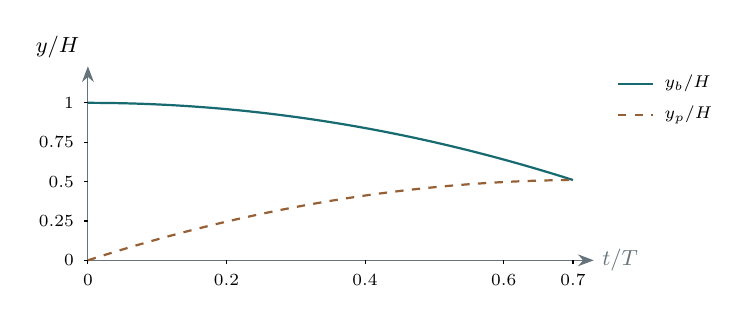
\begin{tikzpicture}[scale=.88,transform shape]
\draw[axis] (0,0.0)--(7.3,0.0) node[right] {$t/T$};
\draw[axis] (0,0)--(0,2.8);
\node[above left] at (0,2.8) {$y/H$};
\draw[thin] (0.000000,0.0)--(0.000000,-0.06);\node[below,font=\scriptsize] at (0.000000,-0.08) {$ 0 $};
\draw[thin] (2.000000,0.0)--(2.000000,-0.06);\node[below,font=\scriptsize] at (2.000000,-0.08) {$ 0.2 $};
\draw[thin] (4.000000,0.0)--(4.000000,-0.06);\node[below,font=\scriptsize] at (4.000000,-0.08) {$ 0.4 $};
\draw[thin] (6.000000,0.0)--(6.000000,-0.06);\node[below,font=\scriptsize] at (6.000000,-0.08) {$ 0.6 $};
\draw[thin] (7.000000,0.0)--(7.000000,-0.06);\node[below,font=\scriptsize] at (7.000000,-0.08) {$ 0.7 $};
\draw[thin] (0,0.000000)--(-.06,0.000000);\node[left,font=\scriptsize] at (-.08,0.000000) {$ 0 $};
\draw[thin] (0,0.568182)--(-.06,0.568182);\node[left,font=\scriptsize] at (-.08,0.568182) {$ 0.25 $};
\draw[thin] (0,1.136364)--(-.06,1.136364);\node[left,font=\scriptsize] at (-.08,1.136364) {$ 0.5 $};
\draw[thin] (0,1.704545)--(-.06,1.704545);\node[left,font=\scriptsize] at (-.08,1.704545) {$ 0.75 $};
\draw[thin] (0,2.272727)--(-.06,2.272727);\node[left,font=\scriptsize] at (-.08,2.272727) {$ 1 $};
\draw[thick,color=accent] plot coordinates {(0.0000000,2.2727273) (0.0291667,2.2727079) (0.0583333,2.2726499) (0.0875000,2.2725533) (0.1166667,2.2724179) (0.1458333,2.2722439) (0.1750000,2.2720312) (0.2041667,2.2717799) (0.2333333,2.2714899) (0.2625000,2.2711612) (0.2916667,2.2707939) (0.3208333,2.2703879) (0.3500000,2.2699432) (0.3791667,2.2694598) (0.4083333,2.2689378) (0.4375000,2.2683771) (0.4666667,2.2677778) (0.4958333,2.2671398) (0.5250000,2.2664631) (0.5541667,2.2657477) (0.5833333,2.2649937) (0.6125000,2.2642010) (0.6416667,2.2633696) (0.6708333,2.2624996) (0.7000000,2.2615909) (0.7291667,2.2606435) (0.7583333,2.2596575) (0.7875000,2.2586328) (0.8166667,2.2575694) (0.8458333,2.2564674) (0.8750000,2.2553267) (0.9041667,2.2541473) (0.9333333,2.2529293) (0.9625000,2.2516726) (0.9916667,2.2503772) (1.0208333,2.2490432) (1.0500000,2.2476705) (1.0791667,2.2462591) (1.1083333,2.2448090) (1.1375000,2.2433203) (1.1666667,2.2417929) (1.1958333,2.2402269) (1.2250000,2.2386222) (1.2541667,2.2369788) (1.2833333,2.2352967) (1.3125000,2.2335760) (1.3416667,2.2318166) (1.3708333,2.2300185) (1.4000000,2.2281818) (1.4291667,2.2263064) (1.4583333,2.2243924) (1.4875000,2.2224396) (1.5166667,2.2204482) (1.5458333,2.2184182) (1.5750000,2.2163494) (1.6041667,2.2142420) (1.6333333,2.2120960) (1.6625000,2.2099112) (1.6916667,2.2076878) (1.7208333,2.2054257) (1.7500000,2.2031250) (1.7791667,2.2007856) (1.8083333,2.1984075) (1.8375000,2.1959908) (1.8666667,2.1935354) (1.8958333,2.1910413) (1.9250000,2.1885085) (1.9541667,2.1859371) (1.9833333,2.1833270) (2.0125000,2.1806783) (2.0416667,2.1779908) (2.0708333,2.1752648) (2.1000000,2.1725000) (2.1291667,2.1696966) (2.1583333,2.1668545) (2.1875000,2.1639737) (2.2166667,2.1610543) (2.2458333,2.1580962) (2.2750000,2.1550994) (2.3041667,2.1520640) (2.3333333,2.1489899) (2.3625000,2.1458771) (2.3916667,2.1427257) (2.4208333,2.1395356) (2.4500000,2.1363068) (2.4791667,2.1330394) (2.5083333,2.1297333) (2.5375000,2.1263885) (2.5666667,2.1230051) (2.5958333,2.1195829) (2.6250000,2.1161222) (2.6541667,2.1126227) (2.6833333,2.1090846) (2.7125000,2.1055078) (2.7416667,2.1018924) (2.7708333,2.0982382) (2.8000000,2.0945455) (2.8291667,2.0908140) (2.8583333,2.0870439) (2.8875000,2.0832351) (2.9166667,2.0793876) (2.9458333,2.0755015) (2.9750000,2.0715767) (3.0041667,2.0676132) (3.0333333,2.0636111) (3.0625000,2.0595703) (3.0916667,2.0554908) (3.1208333,2.0513727) (3.1500000,2.0472159) (3.1791667,2.0430204) (3.2083333,2.0387863) (3.2375000,2.0345135) (3.2666667,2.0302020) (3.2958333,2.0258519) (3.3250000,2.0214631) (3.3541667,2.0170356) (3.3833333,2.0125694) (3.4125000,2.0080646) (3.4416667,2.0035211) (3.4708333,1.9989390) (3.5000000,1.9943182) (3.5291667,1.9896587) (3.5583333,1.9849605) (3.5875000,1.9802237) (3.6166667,1.9754482) (3.6458333,1.9706341) (3.6750000,1.9657812) (3.7041667,1.9608898) (3.7333333,1.9559596) (3.7625000,1.9509908) (3.7916667,1.9459833) (3.8208333,1.9409371) (3.8500000,1.9358523) (3.8791667,1.9307288) (3.9083333,1.9255666) (3.9375000,1.9203658) (3.9666667,1.9151263) (3.9958333,1.9098481) (4.0250000,1.9045313) (4.0541667,1.8991757) (4.0833333,1.8937816) (4.1125000,1.8883487) (4.1416667,1.8828772) (4.1708333,1.8773670) (4.2000000,1.8718182) (4.2291667,1.8662307) (4.2583333,1.8606045) (4.2875000,1.8549396) (4.3166667,1.8492361) (4.3458333,1.8434939) (4.3750000,1.8377131) (4.4041667,1.8318935) (4.4333333,1.8260354) (4.4625000,1.8201385) (4.4916667,1.8142030) (4.5208333,1.8082288) (4.5500000,1.8022159) (4.5791667,1.7961644) (4.6083333,1.7900742) (4.6375000,1.7839453) (4.6666667,1.7777778) (4.6958333,1.7715716) (4.7250000,1.7653267) (4.7541667,1.7590432) (4.7833333,1.7527210) (4.8125000,1.7463601) (4.8416667,1.7399605) (4.8708333,1.7335223) (4.9000000,1.7270455) (4.9291667,1.7205299) (4.9583333,1.7139757) (4.9875000,1.7073828) (5.0166667,1.7007513) (5.0458333,1.6940810) (5.0750000,1.6873722) (5.1041667,1.6806246) (5.1333333,1.6738384) (5.1625000,1.6670135) (5.1916667,1.6601499) (5.2208333,1.6532477) (5.2500000,1.6463068) (5.2791667,1.6393273) (5.3083333,1.6323090) (5.3375000,1.6252521) (5.3666667,1.6181566) (5.3958333,1.6110223) (5.4250000,1.6038494) (5.4541667,1.5966379) (5.4833333,1.5893876) (5.5125000,1.5820987) (5.5416667,1.5747711) (5.5708333,1.5674049) (5.6000000,1.5600000) (5.6291667,1.5525564) (5.6583333,1.5450742) (5.6875000,1.5375533) (5.7166667,1.5299937) (5.7458333,1.5223954) (5.7750000,1.5147585) (5.8041667,1.5070829) (5.8333333,1.4993687) (5.8625000,1.4916158) (5.8916667,1.4838242) (5.9208333,1.4759939) (5.9500000,1.4681250) (5.9791667,1.4602174) (6.0083333,1.4522711) (6.0375000,1.4442862) (6.0666667,1.4362626) (6.0958333,1.4282004) (6.1250000,1.4200994) (6.1541667,1.4119598) (6.1833333,1.4037816) (6.2125000,1.3955646) (6.2416667,1.3873090) (6.2708333,1.3790148) (6.3000000,1.3706818) (6.3291667,1.3623102) (6.3583333,1.3538999) (6.3875000,1.3454510) (6.4166667,1.3369634) (6.4458333,1.3284371) (6.4750000,1.3198722) (6.5041667,1.3112685) (6.5333333,1.3026263) (6.5625000,1.2939453) (6.5916667,1.2852257) (6.6208333,1.2764674) (6.6500000,1.2676705) (6.6791667,1.2588348) (6.7083333,1.2499605) (6.7375000,1.2410476) (6.7666667,1.2320960) (6.7958333,1.2231057) (6.8250000,1.2140767) (6.8541667,1.2050091) (6.8833333,1.1959028) (6.9125000,1.1867578) (6.9416667,1.1775742) (6.9708333,1.1683519) (7.0000000,1.1590909)};
\draw[thick,color=accent] (7.65,2.55)--(8.15,2.55);\node[right,font=\scriptsize] at (8.2,2.55) {$y_b/H$};
\draw[thick,dashed,color=warm] plot coordinates {(0.0000000,0.0000000) (0.0291667,0.0094504) (0.0583333,0.0188621) (0.0875000,0.0282351) (0.1166667,0.0375694) (0.1458333,0.0468651) (0.1750000,0.0561222) (0.2041667,0.0653405) (0.2333333,0.0745202) (0.2625000,0.0836612) (0.2916667,0.0927636) (0.3208333,0.1018273) (0.3500000,0.1108523) (0.3791667,0.1198386) (0.4083333,0.1287863) (0.4375000,0.1376953) (0.4666667,0.1465657) (0.4958333,0.1553973) (0.5250000,0.1641903) (0.5541667,0.1729447) (0.5833333,0.1816604) (0.6125000,0.1903374) (0.6416667,0.1989757) (0.6708333,0.2075754) (0.7000000,0.2161364) (0.7291667,0.2246587) (0.7583333,0.2331424) (0.7875000,0.2415874) (0.8166667,0.2499937) (0.8458333,0.2583613) (0.8750000,0.2666903) (0.9041667,0.2749807) (0.9333333,0.2832323) (0.9625000,0.2914453) (0.9916667,0.2996196) (1.0208333,0.3077553) (1.0500000,0.3158523) (1.0791667,0.3239106) (1.1083333,0.3319302) (1.1375000,0.3399112) (1.1666667,0.3478535) (1.1958333,0.3557572) (1.2250000,0.3636222) (1.2541667,0.3714485) (1.2833333,0.3792361) (1.3125000,0.3869851) (1.3416667,0.3946954) (1.3708333,0.4023670) (1.4000000,0.4100000) (1.4291667,0.4175943) (1.4583333,0.4251499) (1.4875000,0.4326669) (1.5166667,0.4401452) (1.5458333,0.4475848) (1.5750000,0.4549858) (1.6041667,0.4623481) (1.6333333,0.4696717) (1.6625000,0.4769567) (1.6916667,0.4842030) (1.7208333,0.4914106) (1.7500000,0.4985795) (1.7791667,0.5057098) (1.8083333,0.5128015) (1.8375000,0.5198544) (1.8666667,0.5268687) (1.8958333,0.5338443) (1.9250000,0.5407812) (1.9541667,0.5476795) (1.9833333,0.5545391) (2.0125000,0.5613601) (2.0416667,0.5681424) (2.0708333,0.5748860) (2.1000000,0.5815909) (2.1291667,0.5882572) (2.1583333,0.5948848) (2.1875000,0.6014737) (2.2166667,0.6080240) (2.2458333,0.6145356) (2.2750000,0.6210085) (2.3041667,0.6274428) (2.3333333,0.6338384) (2.3625000,0.6401953) (2.3916667,0.6465136) (2.4208333,0.6527932) (2.4500000,0.6590341) (2.4791667,0.6652363) (2.5083333,0.6713999) (2.5375000,0.6775249) (2.5666667,0.6836111) (2.5958333,0.6896587) (2.6250000,0.6956676) (2.6541667,0.7016379) (2.6833333,0.7075694) (2.7125000,0.7134624) (2.7416667,0.7193166) (2.7708333,0.7251322) (2.8000000,0.7309091) (2.8291667,0.7366473) (2.8583333,0.7423469) (2.8875000,0.7480078) (2.9166667,0.7536301) (2.9458333,0.7592136) (2.9750000,0.7647585) (3.0041667,0.7702648) (3.0333333,0.7757323) (3.0625000,0.7811612) (3.0916667,0.7865515) (3.1208333,0.7919030) (3.1500000,0.7972159) (3.1791667,0.8024901) (3.2083333,0.8077257) (3.2375000,0.8129226) (3.2666667,0.8180808) (3.2958333,0.8232004) (3.3250000,0.8282812) (3.3541667,0.8333235) (3.3833333,0.8383270) (3.4125000,0.8432919) (3.4416667,0.8482181) (3.4708333,0.8531057) (3.5000000,0.8579545) (3.5291667,0.8627648) (3.5583333,0.8675363) (3.5875000,0.8722692) (3.6166667,0.8769634) (3.6458333,0.8816189) (3.6750000,0.8862358) (3.7041667,0.8908140) (3.7333333,0.8953535) (3.7625000,0.8998544) (3.7916667,0.9043166) (3.8208333,0.9087401) (3.8500000,0.9131250) (3.8791667,0.9174712) (3.9083333,0.9217787) (3.9375000,0.9260476) (3.9666667,0.9302778) (3.9958333,0.9344693) (4.0250000,0.9386222) (4.0541667,0.9427363) (4.0833333,0.9468119) (4.1125000,0.9508487) (4.1416667,0.9548469) (4.1708333,0.9588064) (4.2000000,0.9627273) (4.2291667,0.9666095) (4.2583333,0.9704530) (4.2875000,0.9742578) (4.3166667,0.9780240) (4.3458333,0.9817515) (4.3750000,0.9854403) (4.4041667,0.9890905) (4.4333333,0.9927020) (4.4625000,0.9962749) (4.4916667,0.9998090) (4.5208333,1.0033045) (4.5500000,1.0067614) (4.5791667,1.0101795) (4.6083333,1.0135590) (4.6375000,1.0168999) (4.6666667,1.0202020) (4.6958333,1.0234655) (4.7250000,1.0266903) (4.7541667,1.0298765) (4.7833333,1.0330240) (4.8125000,1.0361328) (4.8416667,1.0392030) (4.8708333,1.0422345) (4.9000000,1.0452273) (4.9291667,1.0481814) (4.9583333,1.0510969) (4.9875000,1.0539737) (5.0166667,1.0568119) (5.0458333,1.0596113) (5.0750000,1.0623722) (5.1041667,1.0650943) (5.1333333,1.0677778) (5.1625000,1.0704226) (5.1916667,1.0730287) (5.2208333,1.0755962) (5.2500000,1.0781250) (5.2791667,1.0806151) (5.3083333,1.0830666) (5.3375000,1.0854794) (5.3666667,1.0878535) (5.3958333,1.0901890) (5.4250000,1.0924858) (5.4541667,1.0947439) (5.4833333,1.0969634) (5.5125000,1.0991442) (5.5416667,1.1012863) (5.5708333,1.1033898) (5.6000000,1.1054545) (5.6291667,1.1074807) (5.6583333,1.1094681) (5.6875000,1.1114169) (5.7166667,1.1133270) (5.7458333,1.1151985) (5.7750000,1.1170313) (5.8041667,1.1188254) (5.8333333,1.1205808) (5.8625000,1.1222976) (5.8916667,1.1239757) (5.9208333,1.1256151) (5.9500000,1.1272159) (5.9791667,1.1287780) (6.0083333,1.1303015) (6.0375000,1.1317862) (6.0666667,1.1332323) (6.0958333,1.1346398) (6.1250000,1.1360085) (6.1541667,1.1373386) (6.1833333,1.1386301) (6.2125000,1.1398828) (6.2416667,1.1410969) (6.2708333,1.1422723) (6.3000000,1.1434091) (6.3291667,1.1445072) (6.3583333,1.1455666) (6.3875000,1.1465874) (6.4166667,1.1475694) (6.4458333,1.1485129) (6.4750000,1.1494176) (6.5041667,1.1502837) (6.5333333,1.1511111) (6.5625000,1.1518999) (6.5916667,1.1526499) (6.6208333,1.1533613) (6.6500000,1.1540341) (6.6791667,1.1546682) (6.7083333,1.1552636) (6.7375000,1.1558203) (6.7666667,1.1563384) (6.7958333,1.1568178) (6.8250000,1.1572585) (6.8541667,1.1576606) (6.8833333,1.1580240) (6.9125000,1.1583487) (6.9416667,1.1586348) (6.9708333,1.1588822) (7.0000000,1.1590909)};
\draw[thick,dashed,color=warm] (7.65,2.0999999999999996)--(8.15,2.0999999999999996);\node[right,font=\scriptsize] at (8.2,2.0999999999999996) {$y_p/H$};
\end{tikzpicture}
\figcaption{变图力试1.1V7\quad 共同水平加速度下两弹在0.7T达到同一高度}
\end{minipage}\end{center}
\item \textbf{给定速度的两个发射方案。}沿用变式1，给定$v_2=2$，求全部落地前相遇时刻与发射角。

令$s=1/t$，速度平方等式为$(a^2+H^2)s^2-2v_1as+v_1^2-v_2^2=0$。代入给定值，
\[
 5s^2-16s+12=0,\qquad s=2\ \text{或}\ 6/5.
\]
两根均大于$1/T$，所以$t=1/2$或$5/6$。前者$(u_x,u_y)=(0,2)$、$\alpha=90^\circ$；后者$(8/5,6/5)$、$\alpha=\arctan(3/4)\simeq36.87^\circ$。碰撞高度分别为$3/4$和$11/36$，均为正。变图力试1.1V8画速度曲线与水平线$v_2=2$的两个交点。
\begin{center}\begin{minipage}{.98\linewidth}\centering
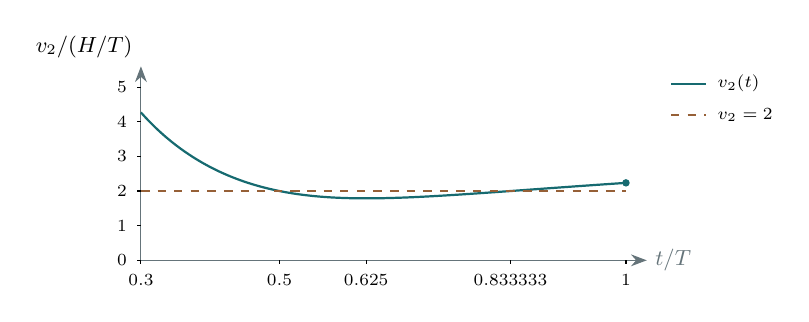
\begin{tikzpicture}[scale=.88,transform shape]
\draw[axis] (0,0.0)--(7.3,0.0) node[right] {$t/T$};
\draw[axis] (0,0)--(0,2.8);
\node[above left] at (0,2.8) {$v_2/(H/T)$};
\draw[thin] (0.000000,0.0)--(0.000000,-0.06);\node[below,font=\scriptsize] at (0.000000,-0.08) {$ 0.3 $};
\draw[thin] (2.000000,0.0)--(2.000000,-0.06);\node[below,font=\scriptsize] at (2.000000,-0.08) {$ 0.5 $};
\draw[thin] (3.250000,0.0)--(3.250000,-0.06);\node[below,font=\scriptsize] at (3.250000,-0.08) {$ 0.625 $};
\draw[thin] (5.333333,0.0)--(5.333333,-0.06);\node[below,font=\scriptsize] at (5.333333,-0.08) {$ 0.833333 $};
\draw[thin] (7.000000,0.0)--(7.000000,-0.06);\node[below,font=\scriptsize] at (7.000000,-0.08) {$ 1 $};
\draw[thin] (0,0.000000)--(-.06,0.000000);\node[left,font=\scriptsize] at (-.08,0.000000) {$ 0 $};
\draw[thin] (0,0.500000)--(-.06,0.500000);\node[left,font=\scriptsize] at (-.08,0.500000) {$ 1 $};
\draw[thin] (0,1.000000)--(-.06,1.000000);\node[left,font=\scriptsize] at (-.08,1.000000) {$ 2 $};
\draw[thin] (0,1.500000)--(-.06,1.500000);\node[left,font=\scriptsize] at (-.08,1.500000) {$ 3 $};
\draw[thin] (0,2.000000)--(-.06,2.000000);\node[left,font=\scriptsize] at (-.08,2.000000) {$ 4 $};
\draw[thin] (0,2.500000)--(-.06,2.500000);\node[left,font=\scriptsize] at (-.08,2.500000) {$ 5 $};
\draw[thick,color=accent] plot coordinates {(0.0000000,2.1343747) (0.0291667,2.1018476) (0.0583333,2.0700486) (0.0875000,2.0389590) (0.1166667,2.0085607) (0.1458333,1.9788363) (0.1750000,1.9497691) (0.2041667,1.9213430) (0.2333333,1.8935425) (0.2625000,1.8663527) (0.2916667,1.8397592) (0.3208333,1.8137482) (0.3500000,1.7883064) (0.3791667,1.7634208) (0.4083333,1.7390791) (0.4375000,1.7152693) (0.4666667,1.6919799) (0.4958333,1.6691996) (0.5250000,1.6469179) (0.5541667,1.6251241) (0.5833333,1.6038083) (0.6125000,1.5829608) (0.6416667,1.5625722) (0.6708333,1.5426333) (0.7000000,1.5231354) (0.7291667,1.5040700) (0.7583333,1.4854287) (0.7875000,1.4672037) (0.8166667,1.4493870) (0.8458333,1.4319713) (0.8750000,1.4149492) (0.9041667,1.3983136) (0.9333333,1.3820576) (0.9625000,1.3661746) (0.9916667,1.3506581) (1.0208333,1.3355017) (1.0500000,1.3206992) (1.0791667,1.3062447) (1.1083333,1.2921322) (1.1375000,1.2783562) (1.1666667,1.2649111) (1.1958333,1.2517913) (1.2250000,1.2389917) (1.2541667,1.2265069) (1.2833333,1.2143320) (1.3125000,1.2024619) (1.3416667,1.1908919) (1.3708333,1.1796170) (1.4000000,1.1686327) (1.4291667,1.1579344) (1.4583333,1.1475174) (1.4875000,1.1373774) (1.5166667,1.1275101) (1.5458333,1.1179110) (1.5750000,1.1085760) (1.6041667,1.0995010) (1.6333333,1.0906816) (1.6625000,1.0821141) (1.6916667,1.0737942) (1.7208333,1.0657180) (1.7500000,1.0578816) (1.7791667,1.0502812) (1.8083333,1.0429129) (1.8375000,1.0357729) (1.8666667,1.0288574) (1.8958333,1.0221627) (1.9250000,1.0156852) (1.9541667,1.0094211) (1.9833333,1.0033668) (2.0125000,0.9975187) (2.0416667,0.9918733) (2.0708333,0.9864269) (2.1000000,0.9811762) (2.1291667,0.9761175) (2.1583333,0.9712474) (2.1875000,0.9665625) (2.2166667,0.9620593) (2.2458333,0.9577345) (2.2750000,0.9535847) (2.3041667,0.9496065) (2.3333333,0.9457966) (2.3625000,0.9421518) (2.3916667,0.9386688) (2.4208333,0.9353443) (2.4500000,0.9321751) (2.4791667,0.9291581) (2.5083333,0.9262900) (2.5375000,0.9235679) (2.5666667,0.9209885) (2.5958333,0.9185487) (2.6250000,0.9162457) (2.6541667,0.9140763) (2.6833333,0.9120376) (2.7125000,0.9101266) (2.7416667,0.9083405) (2.7708333,0.9066764) (2.8000000,0.9051314) (2.8291667,0.9037027) (2.8583333,0.9023875) (2.8875000,0.9011832) (2.9166667,0.9000871) (2.9458333,0.8990964) (2.9750000,0.8982085) (3.0041667,0.8974210) (3.0333333,0.8967312) (3.0625000,0.8961367) (3.0916667,0.8956349) (3.1208333,0.8952235) (3.1500000,0.8949000) (3.1791667,0.8946622) (3.2083333,0.8945078) (3.2375000,0.8944344) (3.2666667,0.8944398) (3.2958333,0.8945220) (3.3250000,0.8946787) (3.3541667,0.8949078) (3.3833333,0.8952073) (3.4125000,0.8955752) (3.4416667,0.8960095) (3.4708333,0.8965082) (3.5000000,0.8970695) (3.5291667,0.8976915) (3.5583333,0.8983724) (3.5875000,0.8991104) (3.6166667,0.8999038) (3.6458333,0.9007508) (3.6750000,0.9016499) (3.7041667,0.9025993) (3.7333333,0.9035976) (3.7625000,0.9046431) (3.7916667,0.9057343) (3.8208333,0.9068697) (3.8500000,0.9080480) (3.8791667,0.9092676) (3.9083333,0.9105273) (3.9375000,0.9118257) (3.9666667,0.9131614) (3.9958333,0.9145332) (4.0250000,0.9159398) (4.0541667,0.9173801) (4.0833333,0.9188529) (4.1125000,0.9203570) (4.1416667,0.9218912) (4.1708333,0.9234545) (4.2000000,0.9250459) (4.2291667,0.9266642) (4.2583333,0.9283085) (4.2875000,0.9299779) (4.3166667,0.9316712) (4.3458333,0.9333877) (4.3750000,0.9351264) (4.4041667,0.9368864) (4.4333333,0.9386669) (4.4625000,0.9404670) (4.4916667,0.9422860) (4.5208333,0.9441230) (4.5500000,0.9459773) (4.5791667,0.9478481) (4.6083333,0.9497348) (4.6375000,0.9516365) (4.6666667,0.9535527) (4.6958333,0.9554827) (4.7250000,0.9574257) (4.7541667,0.9593813) (4.7833333,0.9613488) (4.8125000,0.9633276) (4.8416667,0.9653171) (4.8708333,0.9673167) (4.9000000,0.9693261) (4.9291667,0.9713445) (4.9583333,0.9733715) (4.9875000,0.9754066) (5.0166667,0.9774494) (5.0458333,0.9794993) (5.0750000,0.9815560) (5.1041667,0.9836189) (5.1333333,0.9856877) (5.1625000,0.9877619) (5.1916667,0.9898412) (5.2208333,0.9919251) (5.2500000,0.9940133) (5.2791667,0.9961054) (5.3083333,0.9982011) (5.3375000,1.0003000) (5.3666667,1.0024018) (5.3958333,1.0045062) (5.4250000,1.0066129) (5.4541667,1.0087215) (5.4833333,1.0108318) (5.5125000,1.0129434) (5.5416667,1.0150562) (5.5708333,1.0171698) (5.6000000,1.0192840) (5.6291667,1.0213986) (5.6583333,1.0235133) (5.6875000,1.0256278) (5.7166667,1.0277420) (5.7458333,1.0298556) (5.7750000,1.0319685) (5.8041667,1.0340803) (5.8333333,1.0361910) (5.8625000,1.0383002) (5.8916667,1.0404080) (5.9208333,1.0425140) (5.9500000,1.0446180) (5.9791667,1.0467201) (6.0083333,1.0488198) (6.0375000,1.0509172) (6.0666667,1.0530120) (6.0958333,1.0551042) (6.1250000,1.0571935) (6.1541667,1.0592799) (6.1833333,1.0613631) (6.2125000,1.0634432) (6.2416667,1.0655199) (6.2708333,1.0675931) (6.3000000,1.0696628) (6.3291667,1.0717288) (6.3583333,1.0737910) (6.3875000,1.0758494) (6.4166667,1.0779037) (6.4458333,1.0799540) (6.4750000,1.0820001) (6.5041667,1.0840420) (6.5333333,1.0860795) (6.5625000,1.0881126) (6.5916667,1.0901412) (6.6208333,1.0921653) (6.6500000,1.0941847) (6.6791667,1.0961994) (6.7083333,1.0982094) (6.7375000,1.1002145) (6.7666667,1.1022147) (6.7958333,1.1042100) (6.8250000,1.1062003) (6.8541667,1.1081855) (6.8833333,1.1101656) (6.9125000,1.1121405) (6.9416667,1.1141103) (6.9708333,1.1160748) (7.0000000,1.1180340)};
\draw[thick,color=accent] (7.65,2.55)--(8.15,2.55);\node[right,font=\scriptsize] at (8.2,2.55) {$v_2(t)$};
\draw[thick,dashed,color=warm] plot coordinates {(0.0000000,1.0000000) (0.0291667,1.0000000) (0.0583333,1.0000000) (0.0875000,1.0000000) (0.1166667,1.0000000) (0.1458333,1.0000000) (0.1750000,1.0000000) (0.2041667,1.0000000) (0.2333333,1.0000000) (0.2625000,1.0000000) (0.2916667,1.0000000) (0.3208333,1.0000000) (0.3500000,1.0000000) (0.3791667,1.0000000) (0.4083333,1.0000000) (0.4375000,1.0000000) (0.4666667,1.0000000) (0.4958333,1.0000000) (0.5250000,1.0000000) (0.5541667,1.0000000) (0.5833333,1.0000000) (0.6125000,1.0000000) (0.6416667,1.0000000) (0.6708333,1.0000000) (0.7000000,1.0000000) (0.7291667,1.0000000) (0.7583333,1.0000000) (0.7875000,1.0000000) (0.8166667,1.0000000) (0.8458333,1.0000000) (0.8750000,1.0000000) (0.9041667,1.0000000) (0.9333333,1.0000000) (0.9625000,1.0000000) (0.9916667,1.0000000) (1.0208333,1.0000000) (1.0500000,1.0000000) (1.0791667,1.0000000) (1.1083333,1.0000000) (1.1375000,1.0000000) (1.1666667,1.0000000) (1.1958333,1.0000000) (1.2250000,1.0000000) (1.2541667,1.0000000) (1.2833333,1.0000000) (1.3125000,1.0000000) (1.3416667,1.0000000) (1.3708333,1.0000000) (1.4000000,1.0000000) (1.4291667,1.0000000) (1.4583333,1.0000000) (1.4875000,1.0000000) (1.5166667,1.0000000) (1.5458333,1.0000000) (1.5750000,1.0000000) (1.6041667,1.0000000) (1.6333333,1.0000000) (1.6625000,1.0000000) (1.6916667,1.0000000) (1.7208333,1.0000000) (1.7500000,1.0000000) (1.7791667,1.0000000) (1.8083333,1.0000000) (1.8375000,1.0000000) (1.8666667,1.0000000) (1.8958333,1.0000000) (1.9250000,1.0000000) (1.9541667,1.0000000) (1.9833333,1.0000000) (2.0125000,1.0000000) (2.0416667,1.0000000) (2.0708333,1.0000000) (2.1000000,1.0000000) (2.1291667,1.0000000) (2.1583333,1.0000000) (2.1875000,1.0000000) (2.2166667,1.0000000) (2.2458333,1.0000000) (2.2750000,1.0000000) (2.3041667,1.0000000) (2.3333333,1.0000000) (2.3625000,1.0000000) (2.3916667,1.0000000) (2.4208333,1.0000000) (2.4500000,1.0000000) (2.4791667,1.0000000) (2.5083333,1.0000000) (2.5375000,1.0000000) (2.5666667,1.0000000) (2.5958333,1.0000000) (2.6250000,1.0000000) (2.6541667,1.0000000) (2.6833333,1.0000000) (2.7125000,1.0000000) (2.7416667,1.0000000) (2.7708333,1.0000000) (2.8000000,1.0000000) (2.8291667,1.0000000) (2.8583333,1.0000000) (2.8875000,1.0000000) (2.9166667,1.0000000) (2.9458333,1.0000000) (2.9750000,1.0000000) (3.0041667,1.0000000) (3.0333333,1.0000000) (3.0625000,1.0000000) (3.0916667,1.0000000) (3.1208333,1.0000000) (3.1500000,1.0000000) (3.1791667,1.0000000) (3.2083333,1.0000000) (3.2375000,1.0000000) (3.2666667,1.0000000) (3.2958333,1.0000000) (3.3250000,1.0000000) (3.3541667,1.0000000) (3.3833333,1.0000000) (3.4125000,1.0000000) (3.4416667,1.0000000) (3.4708333,1.0000000) (3.5000000,1.0000000) (3.5291667,1.0000000) (3.5583333,1.0000000) (3.5875000,1.0000000) (3.6166667,1.0000000) (3.6458333,1.0000000) (3.6750000,1.0000000) (3.7041667,1.0000000) (3.7333333,1.0000000) (3.7625000,1.0000000) (3.7916667,1.0000000) (3.8208333,1.0000000) (3.8500000,1.0000000) (3.8791667,1.0000000) (3.9083333,1.0000000) (3.9375000,1.0000000) (3.9666667,1.0000000) (3.9958333,1.0000000) (4.0250000,1.0000000) (4.0541667,1.0000000) (4.0833333,1.0000000) (4.1125000,1.0000000) (4.1416667,1.0000000) (4.1708333,1.0000000) (4.2000000,1.0000000) (4.2291667,1.0000000) (4.2583333,1.0000000) (4.2875000,1.0000000) (4.3166667,1.0000000) (4.3458333,1.0000000) (4.3750000,1.0000000) (4.4041667,1.0000000) (4.4333333,1.0000000) (4.4625000,1.0000000) (4.4916667,1.0000000) (4.5208333,1.0000000) (4.5500000,1.0000000) (4.5791667,1.0000000) (4.6083333,1.0000000) (4.6375000,1.0000000) (4.6666667,1.0000000) (4.6958333,1.0000000) (4.7250000,1.0000000) (4.7541667,1.0000000) (4.7833333,1.0000000) (4.8125000,1.0000000) (4.8416667,1.0000000) (4.8708333,1.0000000) (4.9000000,1.0000000) (4.9291667,1.0000000) (4.9583333,1.0000000) (4.9875000,1.0000000) (5.0166667,1.0000000) (5.0458333,1.0000000) (5.0750000,1.0000000) (5.1041667,1.0000000) (5.1333333,1.0000000) (5.1625000,1.0000000) (5.1916667,1.0000000) (5.2208333,1.0000000) (5.2500000,1.0000000) (5.2791667,1.0000000) (5.3083333,1.0000000) (5.3375000,1.0000000) (5.3666667,1.0000000) (5.3958333,1.0000000) (5.4250000,1.0000000) (5.4541667,1.0000000) (5.4833333,1.0000000) (5.5125000,1.0000000) (5.5416667,1.0000000) (5.5708333,1.0000000) (5.6000000,1.0000000) (5.6291667,1.0000000) (5.6583333,1.0000000) (5.6875000,1.0000000) (5.7166667,1.0000000) (5.7458333,1.0000000) (5.7750000,1.0000000) (5.8041667,1.0000000) (5.8333333,1.0000000) (5.8625000,1.0000000) (5.8916667,1.0000000) (5.9208333,1.0000000) (5.9500000,1.0000000) (5.9791667,1.0000000) (6.0083333,1.0000000) (6.0375000,1.0000000) (6.0666667,1.0000000) (6.0958333,1.0000000) (6.1250000,1.0000000) (6.1541667,1.0000000) (6.1833333,1.0000000) (6.2125000,1.0000000) (6.2416667,1.0000000) (6.2708333,1.0000000) (6.3000000,1.0000000) (6.3291667,1.0000000) (6.3583333,1.0000000) (6.3875000,1.0000000) (6.4166667,1.0000000) (6.4458333,1.0000000) (6.4750000,1.0000000) (6.5041667,1.0000000) (6.5333333,1.0000000) (6.5625000,1.0000000) (6.5916667,1.0000000) (6.6208333,1.0000000) (6.6500000,1.0000000) (6.6791667,1.0000000) (6.7083333,1.0000000) (6.7375000,1.0000000) (6.7666667,1.0000000) (6.7958333,1.0000000) (6.8250000,1.0000000) (6.8541667,1.0000000) (6.8833333,1.0000000) (6.9125000,1.0000000) (6.9416667,1.0000000) (6.9708333,1.0000000) (7.0000000,1.0000000)};
\draw[thick,dashed,color=warm] (7.65,2.0999999999999996)--(8.15,2.0999999999999996);\node[right,font=\scriptsize] at (8.2,2.0999999999999996) {$v_2=2$};
\draw[fill=white,color=accent] (7.0000000,1.1180340) circle(.045);
\end{tikzpicture}
\figcaption{变图力试1.1V8\quad 给定速度2与时间曲线的两个允许交点}
\end{minipage}\end{center}
\end{enumerate}

\Needspace{13\baselineskip}

\pdfbookmark[2]{第 2 题 可移动圆环内小球的轨迹与曲率}{q2}

\section*{第 2 题\quad 可移动圆环内小球的轨迹与曲率}\label{q:2}


半径为$R$的竖直空心圆环固定在滑块上，环和滑块总质量为$M$，可在光滑水平地面上平移而不转动。质量为$m$的小球视为质点，可在环内的光滑管道中运动。

开始时环与球都静止，球在最高点。用极小扰动使球向右下滑，讨论扰动趋零时的轨迹。以初始环心$O$为地面坐标原点，水平向右为$x$，竖直向上为$y$。求：
\begin{enumerate}
\item 小球相对地面的轨迹方程。
\item 小球经过圆环右侧点$A$及最低点$B$时，地面轨迹的曲率半径。要求用受力与相对运动说明，而不只引用椭圆曲率公式。
\end{enumerate}


\begin{center}\begin{minipage}{.98\linewidth}\centering
\begin{tikzpicture}[scale=.9,transform shape]
\draw[object] (0.00000,0.00000) circle(3.00000);\draw[object] (-1.50000,-3.10000)--(1.50000,-3.10000)--(1.50000,-3.50000)--(-1.50000,-3.50000)--(-1.50000,-3.10000);\draw[object] (-2.00000,-3.65000)--(2.00000,-3.65000);\draw[object] (-1.00000,-2.82843)--(-1.00000,-3.10000);\draw[object] (1.00000,-2.82843)--(1.00000,-3.10000);\fill (0.00000,3.00000) circle(.035);\node[above] at (0.00000,3.00000) {$m$};\fill (3.00000,0.00000) circle(.035);\node[right] at (3.00000,0.00000) {$A$};\fill (0.00000,-3.00000) circle(.035);\node[above right] at (0.00000,-3.00000) {$B$};\fill (0.00000,0.00000) circle(.035);\node[above left] at (0.00000,0.00000) {$O$};\draw[<->,thin,color=muted] (0.00000,-0.40000)--(3.00000,-0.40000);\node[below] at (1.50000,-0.40000) {$R$};\node[below] at (0.00000,-4.00000) {环与滑块总质量 $M$};
\end{tikzpicture}
\figcaption{图力试1.2\quad 球从环顶向右微扰，A为相对圆的右侧点，B为底点。}
\end{minipage}\end{center}

\Needspace{8\baselineskip}

\pdfbookmark[3]{题型定位}{q2-h0}

\subsection*{题型定位}

水平动量守恒的时间积分固定水平质心，将相对圆轨迹化成地面椭圆。A处用环心加速度换算法向加速度，B处用环心速度换算速率，分别通过受力求地面曲率。

\Needspace{8\baselineskip}

\pdfbookmark[3]{知识点}{q2-h1}

\subsection*{知识点}

\begin{itemize}
\item 水平方向外力为零，初始总动量为零，给$mx+MX=0$。
\item 相对坐标$x'=x-X$与圆约束共同确定地面椭圆，水平半轴$kR$，$k=M/(M+m)$。
\item 曲率关系$\rho=v^2/a_n$中的速度、法向加速度取同一地面参考系。
\item 平移参考系满足$\boldsymbol a_{\rm rel}=\boldsymbol a_b-\boldsymbol a_{O'}$，速率由速度矢量相减求出。
\item 微扰趋零选出最高点平衡附近的下滑轨迹，运动时间与空间轨迹分别处理。\end{itemize}

\Needspace{8\baselineskip}

\pdfbookmark[3]{物理图像}{q2-h2}

\subsection*{物理图像}

A图画环心向左移动与球地面横位移缩短的关系，并画固定地面椭圆。B图在右端A分别给球向左的支持力、环向右的加速度和向下球速；C图在底点B画相反的地面速度和竖直合力。D图把两处曲率半径连为随位置变化的曲线。

\Needspace{8\baselineskip}

\pdfbookmark[3]{解题入口}{q2-h3}

\subsection*{解题入口}

先对水平总动量积分求$mx+MX=0$，消去环心位置。求曲率时先在图上定切线和法向，再列球与环的同一时刻速度、受力及加速度；未知速率在两种法向关系的比值中消去。

\Needspace{8\baselineskip}

\pdfbookmark[3]{标准解法}{q2-h4}

\subsection*{标准解法}


图力试1.2以初始环心$O$为地面坐标原点，当前环心记为$O'$，其横坐标为$X$，小球地面坐标为$(x,y)$。环与滑块只作水平平移，球和环的相互作用为内力，地面支持力与重力均竖直，故系统水平方向总动量守恒：
\[
m\dot x+M\dot X=0,\qquad mx+MX=0.
\]
第二式由第一式对时间积分，并用初始$x=X=0$确定积分常量。它也说明系统水平质心始终在$O$的竖直线上。相对环心的坐标$(x',y')$与地面坐标之间满足
\[
x'=x-X=\frac{M+m}{M}x,\qquad y'=y.
\]
解图力试1.2A把圆环向左的位移、球对环的横向位移及球对地面的较小横向位移画在一起。相对位置约束$x'^2+y'^2=R^2$于是变成
\[
\boxed{\frac{x^2}{a^2}+\frac{y^2}{R^2}=1},
\qquad a=\frac{M}{M+m}R<R.
\]
轨迹为竖直半长轴$R$、水平半轴$a$的椭圆。记$k=M/(M+m)$，则$a=kR$，$0<k<1$。以从环顶向右量起的角$\theta$为参数，同一位置关系为
\[
x=a\sin\theta,\quad y=R\cos\theta,\quad
X=-\frac{mR}{M+m}\sin\theta.
\]
球向右的相对位移$R\sin\theta$分成球向右的地面位移$kR\sin\theta$和环向左的位移$(1-k)R\sin\theta$，两项相加恢复相对横向距离。
\begin{center}\begin{minipage}{.98\linewidth}\centering
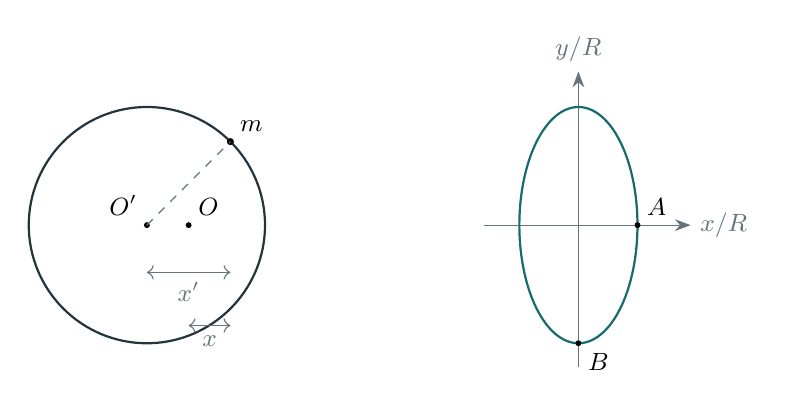
\begin{tikzpicture}[scale=1.5]
\draw[object] (-0.3535534,0) circle(1);
\fill (-0.3535534,0) circle(.025) node[above left] {$O^\prime$};
\fill (0,0) circle(.025) node[above right] {$O$};
\fill (0.3535534,0.7071068) circle(.03) node[above right] {$m$};
\draw[guide] (-0.3535534,0)--(0.3535534,0.7071068);
\draw[<->,thin,color=muted] (-0.3535534,-.4)--(0.3535534,-.4) node[midway,below] {$x^\prime$};
\draw[<->,thin,color=muted] (0,-.85)--(0.3535534,-.85) node[midway,below] {$x$};
\begin{scope}[shift={(3.3,0)}]
\draw[axis] (-.8,0)--(.95,0) node[right] {$x/R$};\draw[axis] (0,-1.2)--(0,1.3) node[above] {$y/R$};
\draw[traj] plot coordinates {(0.0000000,1.0000000) (0.0130885,0.9996573) (0.0261680,0.9986295) (0.0392295,0.9969173) (0.0522642,0.9945219) (0.0652631,0.9914449) (0.0782172,0.9876883) (0.0911178,0.9832549) (0.1039558,0.9781476) (0.1167227,0.9723699) (0.1294095,0.9659258) (0.1420077,0.9588197) (0.1545085,0.9510565) (0.1669034,0.9426415) (0.1791840,0.9335804) (0.1913417,0.9238795) (0.2033683,0.9135455) (0.2152555,0.9025853) (0.2269952,0.8910065) (0.2385794,0.8788171) (0.2500000,0.8660254) (0.2612493,0.8526402) (0.2723195,0.8386706) (0.2832031,0.8241262) (0.2938926,0.8090170) (0.3043807,0.7933533) (0.3146602,0.7771460) (0.3247240,0.7604060) (0.3345653,0.7431448) (0.3441773,0.7253744) (0.3535534,0.7071068) (0.3626872,0.6883546) (0.3715724,0.6691306) (0.3802030,0.6494480) (0.3885730,0.6293204) (0.3966767,0.6087614) (0.4045085,0.5877853) (0.4120631,0.5664062) (0.4193353,0.5446390) (0.4263201,0.5224986) (0.4330127,0.5000000) (0.4394086,0.4771588) (0.4455033,0.4539905) (0.4512926,0.4305111) (0.4567727,0.4067366) (0.4619398,0.3826834) (0.4667902,0.3583679) (0.4713207,0.3338069) (0.4755283,0.3090170) (0.4794099,0.2840153) (0.4829629,0.2588190) (0.4861850,0.2334454) (0.4890738,0.2079117) (0.4916275,0.1822355) (0.4938442,0.1564345) (0.4957224,0.1305262) (0.4972609,0.1045285) (0.4984587,0.0784591) (0.4993148,0.0523360) (0.4998287,0.0261769) (0.5000000,0.0000000) (0.4998287,-0.0261769) (0.4993148,-0.0523360) (0.4984587,-0.0784591) (0.4972609,-0.1045285) (0.4957224,-0.1305262) (0.4938442,-0.1564345) (0.4916275,-0.1822355) (0.4890738,-0.2079117) (0.4861850,-0.2334454) (0.4829629,-0.2588190) (0.4794099,-0.2840153) (0.4755283,-0.3090170) (0.4713207,-0.3338069) (0.4667902,-0.3583679) (0.4619398,-0.3826834) (0.4567727,-0.4067366) (0.4512926,-0.4305111) (0.4455033,-0.4539905) (0.4394086,-0.4771588) (0.4330127,-0.5000000) (0.4263201,-0.5224986) (0.4193353,-0.5446390) (0.4120631,-0.5664062) (0.4045085,-0.5877853) (0.3966767,-0.6087614) (0.3885730,-0.6293204) (0.3802030,-0.6494480) (0.3715724,-0.6691306) (0.3626872,-0.6883546) (0.3535534,-0.7071068) (0.3441773,-0.7253744) (0.3345653,-0.7431448) (0.3247240,-0.7604060) (0.3146602,-0.7771460) (0.3043807,-0.7933533) (0.2938926,-0.8090170) (0.2832031,-0.8241262) (0.2723195,-0.8386706) (0.2612493,-0.8526402) (0.2500000,-0.8660254) (0.2385794,-0.8788171) (0.2269952,-0.8910065) (0.2152555,-0.9025853) (0.2033683,-0.9135455) (0.1913417,-0.9238795) (0.1791840,-0.9335804) (0.1669034,-0.9426415) (0.1545085,-0.9510565) (0.1420077,-0.9588197) (0.1294095,-0.9659258) (0.1167227,-0.9723699) (0.1039558,-0.9781476) (0.0911178,-0.9832549) (0.0782172,-0.9876883) (0.0652631,-0.9914449) (0.0522642,-0.9945219) (0.0392295,-0.9969173) (0.0261680,-0.9986295) (0.0130885,-0.9996573) (0.0000000,-1.0000000) (-0.0130885,-0.9996573) (-0.0261680,-0.9986295) (-0.0392295,-0.9969173) (-0.0522642,-0.9945219) (-0.0652631,-0.9914449) (-0.0782172,-0.9876883) (-0.0911178,-0.9832549) (-0.1039558,-0.9781476) (-0.1167227,-0.9723699) (-0.1294095,-0.9659258) (-0.1420077,-0.9588197) (-0.1545085,-0.9510565) (-0.1669034,-0.9426415) (-0.1791840,-0.9335804) (-0.1913417,-0.9238795) (-0.2033683,-0.9135455) (-0.2152555,-0.9025853) (-0.2269952,-0.8910065) (-0.2385794,-0.8788171) (-0.2500000,-0.8660254) (-0.2612493,-0.8526402) (-0.2723195,-0.8386706) (-0.2832031,-0.8241262) (-0.2938926,-0.8090170) (-0.3043807,-0.7933533) (-0.3146602,-0.7771460) (-0.3247240,-0.7604060) (-0.3345653,-0.7431448) (-0.3441773,-0.7253744) (-0.3535534,-0.7071068) (-0.3626872,-0.6883546) (-0.3715724,-0.6691306) (-0.3802030,-0.6494480) (-0.3885730,-0.6293204) (-0.3966767,-0.6087614) (-0.4045085,-0.5877853) (-0.4120631,-0.5664062) (-0.4193353,-0.5446390) (-0.4263201,-0.5224986) (-0.4330127,-0.5000000) (-0.4394086,-0.4771588) (-0.4455033,-0.4539905) (-0.4512926,-0.4305111) (-0.4567727,-0.4067366) (-0.4619398,-0.3826834) (-0.4667902,-0.3583679) (-0.4713207,-0.3338069) (-0.4755283,-0.3090170) (-0.4794099,-0.2840153) (-0.4829629,-0.2588190) (-0.4861850,-0.2334454) (-0.4890738,-0.2079117) (-0.4916275,-0.1822355) (-0.4938442,-0.1564345) (-0.4957224,-0.1305262) (-0.4972609,-0.1045285) (-0.4984587,-0.0784591) (-0.4993148,-0.0523360) (-0.4998287,-0.0261769) (-0.5000000,-0.0000000) (-0.4998287,0.0261769) (-0.4993148,0.0523360) (-0.4984587,0.0784591) (-0.4972609,0.1045285) (-0.4957224,0.1305262) (-0.4938442,0.1564345) (-0.4916275,0.1822355) (-0.4890738,0.2079117) (-0.4861850,0.2334454) (-0.4829629,0.2588190) (-0.4794099,0.2840153) (-0.4755283,0.3090170) (-0.4713207,0.3338069) (-0.4667902,0.3583679) (-0.4619398,0.3826834) (-0.4567727,0.4067366) (-0.4512926,0.4305111) (-0.4455033,0.4539905) (-0.4394086,0.4771588) (-0.4330127,0.5000000) (-0.4263201,0.5224986) (-0.4193353,0.5446390) (-0.4120631,0.5664062) (-0.4045085,0.5877853) (-0.3966767,0.6087614) (-0.3885730,0.6293204) (-0.3802030,0.6494480) (-0.3715724,0.6691306) (-0.3626872,0.6883546) (-0.3535534,0.7071068) (-0.3441773,0.7253744) (-0.3345653,0.7431448) (-0.3247240,0.7604060) (-0.3146602,0.7771460) (-0.3043807,0.7933533) (-0.2938926,0.8090170) (-0.2832031,0.8241262) (-0.2723195,0.8386706) (-0.2612493,0.8526402) (-0.2500000,0.8660254) (-0.2385794,0.8788171) (-0.2269952,0.8910065) (-0.2152555,0.9025853) (-0.2033683,0.9135455) (-0.1913417,0.9238795) (-0.1791840,0.9335804) (-0.1669034,0.9426415) (-0.1545085,0.9510565) (-0.1420077,0.9588197) (-0.1294095,0.9659258) (-0.1167227,0.9723699) (-0.1039558,0.9781476) (-0.0911178,0.9832549) (-0.0782172,0.9876883) (-0.0652631,0.9914449) (-0.0522642,0.9945219) (-0.0392295,0.9969173) (-0.0261680,0.9986295) (-0.0130885,0.9996573) (-0.0000000,1.0000000)};
\fill (.5,0) circle(.025) node[above right] {$A$};\fill (0,-1) circle(.025) node[below right] {$B$};
\end{scope}
\end{tikzpicture}
\figcaption{解图力试1.2A\quad k等于二分之一的示例：相对圆的横位移分成球与环心的反向位移}
\end{minipage}\end{center}
地面曲率由同一参考系的速度和法向加速度确定。曲线在某点的切线给速度方向，垂直切线的加速度分量满足$a_n=v^2/\rho$；重力及支持力各自在法向上的投影决定该处$a_n$。$A$和$B$两点分别用该瞬间的球、环运动列式，将相对速率换成地面速率。

在解图力试1.2B的右端$A$，$\theta=\pi/2$，球在地面椭圆上的速度竖直向下。由参数式求导，$\dot X=-(1-k)R\cos\theta\,\dot\theta=0$，所以球的地面速率与相对环速率相同，记为$v_A$。球受向左的支持力$N_A$和向下的重力$mg$；前者沿地面曲线法向，后者沿切线。环受到向右的水平反作用力，因而
\[
a_{bx}=-\frac{N_A}{m},\qquad \ddot X=\frac{N_A}{M}.
\]
球相对环沿半径$R$的圆运动，水平方向相对加速度是$-v_A^2/R$。用$a_{bx}-\ddot X=-v_A^2/R$得
\[
N_A\left(\frac1m+\frac1M\right)=\frac{v_A^2}{R},
\quad
N_A=\frac{Mm}{M+m}\frac{v_A^2}{R}.
\]
在随环平移的参考系中，同一关系写成$N_A+m\ddot X=mv_A^2/R$：向左的惯性力$m\ddot X$与支持力共同给相对法向加速度。地面法向加速度为$N_A/m$，故
\[
\boxed{\rho_A=\frac{M+m}{M}R=\frac{R^2}{a}}.
\]
环心瞬时速度虽为零，向右加速度却使球相对环的向左加速度比地面系的大。因此地面轨迹在$A$处比相对圆更平，曲率半径大于$R$，与解图A右端形状一致。
\begin{center}\begin{minipage}{.98\linewidth}\centering
\begin{tikzpicture}[scale=.9,transform shape]
\fill (0,0) circle(.045) node[above right] {$A$};
\draw[force] (0,0)--(-2,0) node[above] {$N_A$};
\draw[force] (0,0)--(0,-1.3) node[left] {$mg$};
\draw[motion] (.7,-.1)--(.7,-1.9) node[right] {$v_A=v_{\rm rel,A}$};
\draw[motion] (2.2,1)--(4.2,1) node[above] {$\ddot X=N_A/M$};
\node[above] at (-.4,1) {球的法向向左};\node at (3.2,.2) {环心瞬时速度为零};
\end{tikzpicture}
\figcaption{解图力试1.2B\quad A处重力沿切线，球与环的水平加速度相反}
\end{minipage}\end{center}
在解图力试1.2C的最低点$B$，$\theta=\pi$，球向左、环心向右运动。设地面速率分别为$v_B$和$V_B$。球所受支持力、重力都竖直，环所受球的反作用力也竖直；水平方向反作用力为零，使$\ddot X=0$。水平动量守恒和速度相减给
\[
MV_B=mv_B,\qquad
v_{\mathrm{rel},B}=v_B+V_B=\frac{M+m}{M}v_B.
\]
相对速率是两相反方向地面速率之和。此时地面曲线与相对圆的切线都水平、法向都竖直；又因环无竖直运动，两个系的竖直加速度相同，所以
\[
N_B-mg=m\frac{v_B^2}{\rho_B}
=m\frac{v_{\mathrm{rel},B}^2}{R}.
\]
相同法向加速度对应不同速率，消去支持力后得
\[
\boxed{\rho_B=\left(\frac{M}{M+m}\right)^2R=\frac{a^2}{R}}.
\]
也可直接由两式相除写成$\rho_B=R(v_B/v_{\rm rel,B})^2=k^2R$。$B$处的环心加速度为零而速度为正，速率换算使椭圆底部的地面曲率半径小于$R$。$A$处处理相对加速度，$B$处处理相对速度，二者由各自受力方向与运动瞬间决定。
\begin{center}\begin{minipage}{.98\linewidth}\centering
\begin{tikzpicture}[scale=.9,transform shape]
\draw[guide] (0,2) circle(2);
\fill (0,0) circle(.045) node[below left] {$B$};
\draw[force] (0,0)--(0,1.5) node[right] {$N_B$};
\draw[force] (0,0)--(0,-1.2) node[right] {$mg$};
\draw[motion] (0,-.25)--(-2,-.25) node[above] {$v_B$};
\fill (0,2) circle(.03) node[above left] {$O^\prime$};
\draw[motion] (0,2)--(1.6,2) node[above] {$V_B$};
\node[right] at (2.2,.6) {$v_{\rm rel,B}=v_B+V_B$};\node[right] at (2.2,1.3) {$\ddot X=0$};
\end{tikzpicture}
\figcaption{解图力试1.2C\quad B处两地面速度反向，相对速率为两者之和}
\end{minipage}\end{center}
椭圆参数式还把两个特殊点连成完整的曲率变化。对$\theta$求导有$x_\theta=a\cos\theta$、$y_\theta=-R\sin\theta$、$x_{\theta\theta}=-a\sin\theta$、$y_{\theta\theta}=-R\cos\theta$，行列式绝对值为$aR$，从而
\[
\rho(\theta)=
\frac{(a^2\cos^2\theta+R^2\sin^2\theta)^{3/2}}{aR}.
\]
解图力试1.2D画$\rho/R$随$\theta$的变化，$\theta=\pi/2,\pi$分别回到$R^2/a$和$a^2/R$。这些半径只含质量比与几何量；重力决定小球怎样随时间经过曲线，求$v^2/a_n$时同一速率尺度相消。$M$很大时$k\to1$，地面椭圆趋近圆，两处半径均趋于$R$；减小$M$使横轴收缩，右端更平而底部更尖。
\begin{center}\begin{minipage}{.98\linewidth}\centering
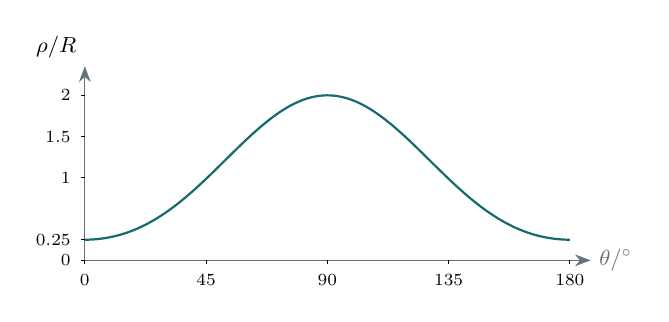
\begin{tikzpicture}[scale=.88,transform shape]
\draw[axis] (0,0.0)--(7.3,0.0) node[right] {$\theta/{}^\circ$};
\draw[axis] (0,0)--(0,2.8);
\node[above left] at (0,2.8) {$\rho/R$};
\draw[thin] (0.000000,0.0)--(0.000000,-0.06);\node[below,font=\scriptsize] at (0.000000,-0.08) {$ 0 $};
\draw[thin] (1.750000,0.0)--(1.750000,-0.06);\node[below,font=\scriptsize] at (1.750000,-0.08) {$ 45 $};
\draw[thin] (3.500000,0.0)--(3.500000,-0.06);\node[below,font=\scriptsize] at (3.500000,-0.08) {$ 90 $};
\draw[thin] (5.250000,0.0)--(5.250000,-0.06);\node[below,font=\scriptsize] at (5.250000,-0.08) {$ 135 $};
\draw[thin] (7.000000,0.0)--(7.000000,-0.06);\node[below,font=\scriptsize] at (7.000000,-0.08) {$ 180 $};
\draw[thin] (0,0.000000)--(-.06,0.000000);\node[left,font=\scriptsize] at (-.08,0.000000) {$ 0 $};
\draw[thin] (0,0.297619)--(-.06,0.297619);\node[left,font=\scriptsize] at (-.08,0.297619) {$ 0.25 $};
\draw[thin] (0,1.190476)--(-.06,1.190476);\node[left,font=\scriptsize] at (-.08,1.190476) {$ 1 $};
\draw[thin] (0,1.785714)--(-.06,1.785714);\node[left,font=\scriptsize] at (-.08,1.785714) {$ 1.5 $};
\draw[thin] (0,2.380952)--(-.06,2.380952);\node[left,font=\scriptsize] at (-.08,2.380952) {$ 2 $};
\draw[thick,color=accent] plot coordinates {(0.0000000,0.2976190) (0.0291667,0.2978485) (0.0583333,0.2985372) (0.0875000,0.2996857) (0.1166667,0.3012949) (0.1458333,0.3033663) (0.1750000,0.3059014) (0.2041667,0.3089024) (0.2333333,0.3123716) (0.2625000,0.3163117) (0.2916667,0.3207257) (0.3208333,0.3256167) (0.3500000,0.3309881) (0.3791667,0.3368435) (0.4083333,0.3431865) (0.4375000,0.3500211) (0.4666667,0.3573509) (0.4958333,0.3651800) (0.5250000,0.3735122) (0.5541667,0.3823513) (0.5833333,0.3917009) (0.6125000,0.4015646) (0.6416667,0.4119458) (0.6708333,0.4228475) (0.7000000,0.4342727) (0.7291667,0.4462238) (0.7583333,0.4587031) (0.7875000,0.4717124) (0.8166667,0.4852532) (0.8458333,0.4993262) (0.8750000,0.5139321) (0.9041667,0.5290707) (0.9333333,0.5447416) (0.9625000,0.5609434) (0.9916667,0.5776746) (1.0208333,0.5949326) (1.0500000,0.6127145) (1.0791667,0.6310167) (1.1083333,0.6498348) (1.1375000,0.6691637) (1.1666667,0.6889977) (1.1958333,0.7093305) (1.2250000,0.7301547) (1.2541667,0.7514625) (1.2833333,0.7732452) (1.3125000,0.7954935) (1.3416667,0.8181972) (1.3708333,0.8413454) (1.4000000,0.8649265) (1.4291667,0.8889281) (1.4583333,0.9133371) (1.4875000,0.9381397) (1.5166667,0.9633212) (1.5458333,0.9888666) (1.5750000,1.0147597) (1.6041667,1.0409839) (1.6333333,1.0675219) (1.6625000,1.0943557) (1.6916667,1.1214667) (1.7208333,1.1488356) (1.7500000,1.1764426) (1.7791667,1.2042672) (1.8083333,1.2322886) (1.8375000,1.2604851) (1.8666667,1.2888347) (1.8958333,1.3173150) (1.9250000,1.3459030) (1.9541667,1.3745752) (1.9833333,1.4033080) (2.0125000,1.4320772) (2.0416667,1.4608582) (2.0708333,1.4896263) (2.1000000,1.5183564) (2.1291667,1.5470232) (2.1583333,1.5756011) (2.1875000,1.6040646) (2.2166667,1.6323876) (2.2458333,1.6605443) (2.2750000,1.6885087) (2.3041667,1.7162547) (2.3333333,1.7437562) (2.3625000,1.7709872) (2.3916667,1.7979218) (2.4208333,1.8245340) (2.4500000,1.8507982) (2.4791667,1.8766889) (2.5083333,1.9021807) (2.5375000,1.9272485) (2.5666667,1.9518675) (2.5958333,1.9760133) (2.6250000,1.9996616) (2.6541667,2.0227888) (2.6833333,2.0453716) (2.7125000,2.0673870) (2.7416667,2.0888126) (2.7708333,2.1096265) (2.8000000,2.1298074) (2.8291667,2.1493346) (2.8583333,2.1681878) (2.8875000,2.1863476) (2.9166667,2.2037950) (2.9458333,2.2205119) (2.9750000,2.2364809) (3.0041667,2.2516851) (3.0333333,2.2661087) (3.0625000,2.2797363) (3.0916667,2.2925538) (3.1208333,2.3045475) (3.1500000,2.3157048) (3.1791667,2.3260137) (3.2083333,2.3354634) (3.2375000,2.3440438) (3.2666667,2.3517458) (3.2958333,2.3585612) (3.3250000,2.3644826) (3.3541667,2.3695038) (3.3833333,2.3736194) (3.4125000,2.3768250) (3.4416667,2.3791172) (3.4708333,2.3804935) (3.5000000,2.3809524) (3.5291667,2.3804935) (3.5583333,2.3791172) (3.5875000,2.3768250) (3.6166667,2.3736194) (3.6458333,2.3695038) (3.6750000,2.3644826) (3.7041667,2.3585612) (3.7333333,2.3517458) (3.7625000,2.3440438) (3.7916667,2.3354634) (3.8208333,2.3260137) (3.8500000,2.3157048) (3.8791667,2.3045475) (3.9083333,2.2925538) (3.9375000,2.2797363) (3.9666667,2.2661087) (3.9958333,2.2516851) (4.0250000,2.2364809) (4.0541667,2.2205119) (4.0833333,2.2037950) (4.1125000,2.1863476) (4.1416667,2.1681878) (4.1708333,2.1493346) (4.2000000,2.1298074) (4.2291667,2.1096265) (4.2583333,2.0888126) (4.2875000,2.0673870) (4.3166667,2.0453716) (4.3458333,2.0227888) (4.3750000,1.9996616) (4.4041667,1.9760133) (4.4333333,1.9518675) (4.4625000,1.9272485) (4.4916667,1.9021807) (4.5208333,1.8766889) (4.5500000,1.8507982) (4.5791667,1.8245340) (4.6083333,1.7979218) (4.6375000,1.7709872) (4.6666667,1.7437562) (4.6958333,1.7162547) (4.7250000,1.6885087) (4.7541667,1.6605443) (4.7833333,1.6323876) (4.8125000,1.6040646) (4.8416667,1.5756011) (4.8708333,1.5470232) (4.9000000,1.5183564) (4.9291667,1.4896263) (4.9583333,1.4608582) (4.9875000,1.4320772) (5.0166667,1.4033080) (5.0458333,1.3745752) (5.0750000,1.3459030) (5.1041667,1.3173150) (5.1333333,1.2888347) (5.1625000,1.2604851) (5.1916667,1.2322886) (5.2208333,1.2042672) (5.2500000,1.1764426) (5.2791667,1.1488356) (5.3083333,1.1214667) (5.3375000,1.0943557) (5.3666667,1.0675219) (5.3958333,1.0409839) (5.4250000,1.0147597) (5.4541667,0.9888666) (5.4833333,0.9633212) (5.5125000,0.9381397) (5.5416667,0.9133371) (5.5708333,0.8889281) (5.6000000,0.8649265) (5.6291667,0.8413454) (5.6583333,0.8181972) (5.6875000,0.7954935) (5.7166667,0.7732452) (5.7458333,0.7514625) (5.7750000,0.7301547) (5.8041667,0.7093305) (5.8333333,0.6889977) (5.8625000,0.6691637) (5.8916667,0.6498348) (5.9208333,0.6310167) (5.9500000,0.6127145) (5.9791667,0.5949326) (6.0083333,0.5776746) (6.0375000,0.5609434) (6.0666667,0.5447416) (6.0958333,0.5290707) (6.1250000,0.5139321) (6.1541667,0.4993262) (6.1833333,0.4852532) (6.2125000,0.4717124) (6.2416667,0.4587031) (6.2708333,0.4462238) (6.3000000,0.4342727) (6.3291667,0.4228475) (6.3583333,0.4119458) (6.3875000,0.4015646) (6.4166667,0.3917009) (6.4458333,0.3823513) (6.4750000,0.3735122) (6.5041667,0.3651800) (6.5333333,0.3573509) (6.5625000,0.3500211) (6.5916667,0.3431865) (6.6208333,0.3368435) (6.6500000,0.3309881) (6.6791667,0.3256167) (6.7083333,0.3207257) (6.7375000,0.3163117) (6.7666667,0.3123716) (6.7958333,0.3089024) (6.8250000,0.3059014) (6.8541667,0.3033663) (6.8833333,0.3012949) (6.9125000,0.2996857) (6.9416667,0.2985372) (6.9708333,0.2978485) (7.0000000,0.2976190)};
\end{tikzpicture}
\figcaption{解图力试1.2D\quad k等于二分之一时地面椭圆的曲率半径}
\end{minipage}\end{center}
题设取最高点微扰趋零的轨迹。最高点完全静止的状态本身是平衡解；微小向右偏离选出下滑方向，得到上面的椭圆轨迹极限。初始时间尺度可随扰动变小而增长，空间轨迹、$A,B$处的速率比与曲率结果保持上述极限。


\Needspace{8\baselineskip}

\pdfbookmark[3]{关键洞察}{q2-h5}

\subsection*{关键洞察}

椭圆形状由水平质心位置与相对圆约束确定，重力决定沿椭圆的时间进程。A处环心速度为零、加速度向右，B处环心加速度为零、速度向右；不同运动量分别进入该点曲率的相对变换。

\Needspace{8\baselineskip}

\pdfbookmark[3]{易错点}{q2-h6}

\subsection*{易错点}

\begin{itemize}
\item 地面横坐标为$kR\sin\theta$，相对环心横坐标为$R\sin\theta$。
\item A处环心受水平反作用力而向右加速，相对向心加速度含这项平移加速度。
\item B处球与环的地面速度反向，相对速率为两速率相加。
\item 地面曲率使用地面速率，环系向心关系使用相对速率，两个式子通过同一受力连接。
\item 最高点微扰趋零时保留空间轨迹的极限，严格静止状态的运动方程仍有平衡解。\end{itemize}

\Needspace{8\baselineskip}

\pdfbookmark[3]{课堂讲解建议}{q2-h7}

\subsection*{课堂讲解建议}

先让学生用水平质心位置判断横轴会收缩多少，再从A图读出相对、地面横位移。讲右端时先标环的反作用力，再写相对加速度；讲底部时先画两根反向速度箭头，再写速率之和。各自消去$N$后，将两个结果放回D图，用$M\gg m$与$M=m$两个质量情形解释曲线形状。最后用能量式求沿途速率，说明几何与时间进程的联系。

\Needspace{8\baselineskip}

\pdfbookmark[3]{变式训练}{q2-h8}

\subsection*{变式训练}

\begin{enumerate}
\item \textbf{相等的质量。}若$M=m$，求椭圆两半轴和$A,B$处曲率半径，并在椭圆上画对应密切圆。

此时$k=1/2$，所以$a=R/2$、竖直半轴$R$，$\rho_A=2R$、$\rho_B=R/4$，二者比为8。变图力试1.2V1取$R=1$，$A=(1/2,0)$处法线向左，密切圆心在$(-3/2,0)$；$B=(0,-1)$处法线向上，圆心在$(0,-3/4)$。两个圆各与椭圆在对应点相切，表示右端较平、底端较尖的曲率差别。
\begin{center}\begin{minipage}{.98\linewidth}\centering
\begin{tikzpicture}[scale=1.3]
\draw[thick,color=muted,dashed] (-1.5,0) circle(2);
\draw[thick,color=warm,dashed] (0,-.75) circle(.25);
\draw[traj] plot coordinates {(0.0000000,1.0000000) (0.0130885,0.9996573) (0.0261680,0.9986295) (0.0392295,0.9969173) (0.0522642,0.9945219) (0.0652631,0.9914449) (0.0782172,0.9876883) (0.0911178,0.9832549) (0.1039558,0.9781476) (0.1167227,0.9723699) (0.1294095,0.9659258) (0.1420077,0.9588197) (0.1545085,0.9510565) (0.1669034,0.9426415) (0.1791840,0.9335804) (0.1913417,0.9238795) (0.2033683,0.9135455) (0.2152555,0.9025853) (0.2269952,0.8910065) (0.2385794,0.8788171) (0.2500000,0.8660254) (0.2612493,0.8526402) (0.2723195,0.8386706) (0.2832031,0.8241262) (0.2938926,0.8090170) (0.3043807,0.7933533) (0.3146602,0.7771460) (0.3247240,0.7604060) (0.3345653,0.7431448) (0.3441773,0.7253744) (0.3535534,0.7071068) (0.3626872,0.6883546) (0.3715724,0.6691306) (0.3802030,0.6494480) (0.3885730,0.6293204) (0.3966767,0.6087614) (0.4045085,0.5877853) (0.4120631,0.5664062) (0.4193353,0.5446390) (0.4263201,0.5224986) (0.4330127,0.5000000) (0.4394086,0.4771588) (0.4455033,0.4539905) (0.4512926,0.4305111) (0.4567727,0.4067366) (0.4619398,0.3826834) (0.4667902,0.3583679) (0.4713207,0.3338069) (0.4755283,0.3090170) (0.4794099,0.2840153) (0.4829629,0.2588190) (0.4861850,0.2334454) (0.4890738,0.2079117) (0.4916275,0.1822355) (0.4938442,0.1564345) (0.4957224,0.1305262) (0.4972609,0.1045285) (0.4984587,0.0784591) (0.4993148,0.0523360) (0.4998287,0.0261769) (0.5000000,0.0000000) (0.4998287,-0.0261769) (0.4993148,-0.0523360) (0.4984587,-0.0784591) (0.4972609,-0.1045285) (0.4957224,-0.1305262) (0.4938442,-0.1564345) (0.4916275,-0.1822355) (0.4890738,-0.2079117) (0.4861850,-0.2334454) (0.4829629,-0.2588190) (0.4794099,-0.2840153) (0.4755283,-0.3090170) (0.4713207,-0.3338069) (0.4667902,-0.3583679) (0.4619398,-0.3826834) (0.4567727,-0.4067366) (0.4512926,-0.4305111) (0.4455033,-0.4539905) (0.4394086,-0.4771588) (0.4330127,-0.5000000) (0.4263201,-0.5224986) (0.4193353,-0.5446390) (0.4120631,-0.5664062) (0.4045085,-0.5877853) (0.3966767,-0.6087614) (0.3885730,-0.6293204) (0.3802030,-0.6494480) (0.3715724,-0.6691306) (0.3626872,-0.6883546) (0.3535534,-0.7071068) (0.3441773,-0.7253744) (0.3345653,-0.7431448) (0.3247240,-0.7604060) (0.3146602,-0.7771460) (0.3043807,-0.7933533) (0.2938926,-0.8090170) (0.2832031,-0.8241262) (0.2723195,-0.8386706) (0.2612493,-0.8526402) (0.2500000,-0.8660254) (0.2385794,-0.8788171) (0.2269952,-0.8910065) (0.2152555,-0.9025853) (0.2033683,-0.9135455) (0.1913417,-0.9238795) (0.1791840,-0.9335804) (0.1669034,-0.9426415) (0.1545085,-0.9510565) (0.1420077,-0.9588197) (0.1294095,-0.9659258) (0.1167227,-0.9723699) (0.1039558,-0.9781476) (0.0911178,-0.9832549) (0.0782172,-0.9876883) (0.0652631,-0.9914449) (0.0522642,-0.9945219) (0.0392295,-0.9969173) (0.0261680,-0.9986295) (0.0130885,-0.9996573) (0.0000000,-1.0000000) (-0.0130885,-0.9996573) (-0.0261680,-0.9986295) (-0.0392295,-0.9969173) (-0.0522642,-0.9945219) (-0.0652631,-0.9914449) (-0.0782172,-0.9876883) (-0.0911178,-0.9832549) (-0.1039558,-0.9781476) (-0.1167227,-0.9723699) (-0.1294095,-0.9659258) (-0.1420077,-0.9588197) (-0.1545085,-0.9510565) (-0.1669034,-0.9426415) (-0.1791840,-0.9335804) (-0.1913417,-0.9238795) (-0.2033683,-0.9135455) (-0.2152555,-0.9025853) (-0.2269952,-0.8910065) (-0.2385794,-0.8788171) (-0.2500000,-0.8660254) (-0.2612493,-0.8526402) (-0.2723195,-0.8386706) (-0.2832031,-0.8241262) (-0.2938926,-0.8090170) (-0.3043807,-0.7933533) (-0.3146602,-0.7771460) (-0.3247240,-0.7604060) (-0.3345653,-0.7431448) (-0.3441773,-0.7253744) (-0.3535534,-0.7071068) (-0.3626872,-0.6883546) (-0.3715724,-0.6691306) (-0.3802030,-0.6494480) (-0.3885730,-0.6293204) (-0.3966767,-0.6087614) (-0.4045085,-0.5877853) (-0.4120631,-0.5664062) (-0.4193353,-0.5446390) (-0.4263201,-0.5224986) (-0.4330127,-0.5000000) (-0.4394086,-0.4771588) (-0.4455033,-0.4539905) (-0.4512926,-0.4305111) (-0.4567727,-0.4067366) (-0.4619398,-0.3826834) (-0.4667902,-0.3583679) (-0.4713207,-0.3338069) (-0.4755283,-0.3090170) (-0.4794099,-0.2840153) (-0.4829629,-0.2588190) (-0.4861850,-0.2334454) (-0.4890738,-0.2079117) (-0.4916275,-0.1822355) (-0.4938442,-0.1564345) (-0.4957224,-0.1305262) (-0.4972609,-0.1045285) (-0.4984587,-0.0784591) (-0.4993148,-0.0523360) (-0.4998287,-0.0261769) (-0.5000000,-0.0000000) (-0.4998287,0.0261769) (-0.4993148,0.0523360) (-0.4984587,0.0784591) (-0.4972609,0.1045285) (-0.4957224,0.1305262) (-0.4938442,0.1564345) (-0.4916275,0.1822355) (-0.4890738,0.2079117) (-0.4861850,0.2334454) (-0.4829629,0.2588190) (-0.4794099,0.2840153) (-0.4755283,0.3090170) (-0.4713207,0.3338069) (-0.4667902,0.3583679) (-0.4619398,0.3826834) (-0.4567727,0.4067366) (-0.4512926,0.4305111) (-0.4455033,0.4539905) (-0.4394086,0.4771588) (-0.4330127,0.5000000) (-0.4263201,0.5224986) (-0.4193353,0.5446390) (-0.4120631,0.5664062) (-0.4045085,0.5877853) (-0.3966767,0.6087614) (-0.3885730,0.6293204) (-0.3802030,0.6494480) (-0.3715724,0.6691306) (-0.3626872,0.6883546) (-0.3535534,0.7071068) (-0.3441773,0.7253744) (-0.3345653,0.7431448) (-0.3247240,0.7604060) (-0.3146602,0.7771460) (-0.3043807,0.7933533) (-0.2938926,0.8090170) (-0.2832031,0.8241262) (-0.2723195,0.8386706) (-0.2612493,0.8526402) (-0.2500000,0.8660254) (-0.2385794,0.8788171) (-0.2269952,0.8910065) (-0.2152555,0.9025853) (-0.2033683,0.9135455) (-0.1913417,0.9238795) (-0.1791840,0.9335804) (-0.1669034,0.9426415) (-0.1545085,0.9510565) (-0.1420077,0.9588197) (-0.1294095,0.9659258) (-0.1167227,0.9723699) (-0.1039558,0.9781476) (-0.0911178,0.9832549) (-0.0782172,0.9876883) (-0.0652631,0.9914449) (-0.0522642,0.9945219) (-0.0392295,0.9969173) (-0.0261680,0.9986295) (-0.0130885,0.9996573) (-0.0000000,1.0000000)};
\fill (.5,0) circle(.03) node[right] {$A$};\fill (0,-1) circle(.03) node[below] {$B$};
\fill (-1.5,0) circle(.025) node[below left] {$C_A$};\fill (0,-.75) circle(.025) node[above left] {$C_B$};
\draw[guide] (-1.5,0)--(.5,0) node[midway,above] {$2R$};
\node[right] at (.9,-1.1) {$\rho_B=R/4$};
\end{tikzpicture}
\figcaption{变图力试1.2V1\quad 相等质量时A、B两个密切圆的半径相差8倍}
\end{minipage}\end{center}
\item \textbf{完整的时间速率。}设$\eta=m/(M+m)=1-k$，推导微扰趋零时任意角度的$\dot\theta^2$。

参数速度为$\dot x=kR\cos\theta\,\dot\theta$、$\dot y=-R\sin\theta\,\dot\theta$、$\dot X=-\eta R\cos\theta\,\dot\theta$。相加两物体动能并用$Mk=m\eta$化简，
\[
 K_{\rm tot}=\tfrac12mR^2(1-\eta\cos^2\theta)\dot\theta^2,\qquad
 \dot\theta^2=\frac{2g(1-\cos\theta)}
 {R(1-\eta\cos^2\theta)}.
\]
能量下降为$mgR(1-\cos\theta)$。变图力试1.2V2取$k=1/2$画$R\dot\theta^2/g$，右端值2、底点值8，分母计入圆环平动的动能。
\begin{center}\begin{minipage}{.98\linewidth}\centering
\begin{tikzpicture}[scale=.88,transform shape]
\draw[axis] (0,0.0)--(7.3,0.0) node[right] {$\theta/{}^\circ$};
\draw[axis] (0,0)--(0,2.8);
\node[above left] at (0,2.8) {$R\dot\theta^2/g$};
\draw[thin] (0.000000,0.0)--(0.000000,-0.06);\node[below,font=\scriptsize] at (0.000000,-0.08) {$ 0 $};
\draw[thin] (1.750000,0.0)--(1.750000,-0.06);\node[below,font=\scriptsize] at (1.750000,-0.08) {$ 45 $};
\draw[thin] (3.500000,0.0)--(3.500000,-0.06);\node[below,font=\scriptsize] at (3.500000,-0.08) {$ 90 $};
\draw[thin] (5.250000,0.0)--(5.250000,-0.06);\node[below,font=\scriptsize] at (5.250000,-0.08) {$ 135 $};
\draw[thin] (7.000000,0.0)--(7.000000,-0.06);\node[below,font=\scriptsize] at (7.000000,-0.08) {$ 180 $};
\draw[thin] (0,0.000000)--(-.06,0.000000);\node[left,font=\scriptsize] at (-.08,0.000000) {$ 0 $};
\draw[thin] (0,0.609756)--(-.06,0.609756);\node[left,font=\scriptsize] at (-.08,0.609756) {$ 2 $};
\draw[thin] (0,1.219512)--(-.06,1.219512);\node[left,font=\scriptsize] at (-.08,1.219512) {$ 4 $};
\draw[thin] (0,1.829268)--(-.06,1.829268);\node[left,font=\scriptsize] at (-.08,1.829268) {$ 6 $};
\draw[thin] (0,2.439024)--(-.06,2.439024);\node[left,font=\scriptsize] at (-.08,2.439024) {$ 8 $};
\draw[thick,color=accent] plot coordinates {(0.0000000,0.0000000) (0.0291667,0.0001045) (0.0583333,0.0004176) (0.0875000,0.0009388) (0.1166667,0.0016667) (0.1458333,0.0025999) (0.1750000,0.0037363) (0.2041667,0.0050735) (0.2333333,0.0066084) (0.2625000,0.0083379) (0.2916667,0.0102583) (0.3208333,0.0123656) (0.3500000,0.0146556) (0.3791667,0.0171235) (0.4083333,0.0197645) (0.4375000,0.0225734) (0.4666667,0.0255450) (0.4958333,0.0286737) (0.5250000,0.0319538) (0.5541667,0.0353796) (0.5833333,0.0389450) (0.6125000,0.0426443) (0.6416667,0.0464712) (0.6708333,0.0504200) (0.7000000,0.0544844) (0.7291667,0.0586586) (0.7583333,0.0629366) (0.7875000,0.0673126) (0.8166667,0.0717808) (0.8458333,0.0763357) (0.8750000,0.0809718) (0.9041667,0.0856837) (0.9333333,0.0904661) (0.9625000,0.0953142) (0.9916667,0.1002231) (1.0208333,0.1051881) (1.0500000,0.1102048) (1.0791667,0.1152690) (1.1083333,0.1203766) (1.1375000,0.1255238) (1.1666667,0.1307069) (1.1958333,0.1359226) (1.2250000,0.1411677) (1.2541667,0.1464391) (1.2833333,0.1517341) (1.3125000,0.1570501) (1.3416667,0.1623847) (1.3708333,0.1677357) (1.4000000,0.1731011) (1.4291667,0.1784792) (1.4583333,0.1838683) (1.4875000,0.1892669) (1.5166667,0.1946738) (1.5458333,0.2000878) (1.5750000,0.2055081) (1.6041667,0.2109337) (1.6333333,0.2163641) (1.6625000,0.2217987) (1.6916667,0.2272371) (1.7208333,0.2326791) (1.7500000,0.2381246) (1.7791667,0.2435735) (1.8083333,0.2490259) (1.8375000,0.2544821) (1.8666667,0.2599424) (1.8958333,0.2654071) (1.9250000,0.2708768) (1.9541667,0.2763520) (1.9833333,0.2818334) (2.0125000,0.2873217) (2.0416667,0.2928179) (2.0708333,0.2983226) (2.1000000,0.3038370) (2.1291667,0.3093620) (2.1583333,0.3148987) (2.1875000,0.3204483) (2.2166667,0.3260118) (2.2458333,0.3315907) (2.2750000,0.3371861) (2.3041667,0.3427994) (2.3333333,0.3484321) (2.3625000,0.3540854) (2.3916667,0.3597609) (2.4208333,0.3654601) (2.4500000,0.3711846) (2.4791667,0.3769358) (2.5083333,0.3827155) (2.5375000,0.3885253) (2.5666667,0.3943669) (2.5958333,0.4002420) (2.6250000,0.4061524) (2.6541667,0.4120997) (2.6833333,0.4180859) (2.7125000,0.4241128) (2.7416667,0.4301823) (2.7708333,0.4362962) (2.8000000,0.4424565) (2.8291667,0.4486652) (2.8583333,0.4549242) (2.8875000,0.4612355) (2.9166667,0.4676013) (2.9458333,0.4740235) (2.9750000,0.4805043) (3.0041667,0.4870458) (3.0333333,0.4936503) (3.0625000,0.5003197) (3.0916667,0.5070565) (3.1208333,0.5138628) (3.1500000,0.5207409) (3.1791667,0.5276932) (3.2083333,0.5347220) (3.2375000,0.5418297) (3.2666667,0.5490186) (3.2958333,0.5562912) (3.3250000,0.5636501) (3.3541667,0.5710976) (3.3833333,0.5786364) (3.4125000,0.5862690) (3.4416667,0.5939981) (3.4708333,0.6018262) (3.5000000,0.6097561) (3.5291667,0.6177905) (3.5583333,0.6259321) (3.5875000,0.6341838) (3.6166667,0.6425483) (3.6458333,0.6510285) (3.6750000,0.6596273) (3.7041667,0.6683477) (3.7333333,0.6771925) (3.7625000,0.6861649) (3.7916667,0.6952679) (3.8208333,0.7045045) (3.8500000,0.7138779) (3.8791667,0.7233911) (3.9083333,0.7330475) (3.9375000,0.7428501) (3.9666667,0.7528023) (3.9958333,0.7629073) (4.0250000,0.7731684) (4.0541667,0.7835890) (4.0833333,0.7941723) (4.1125000,0.8049219) (4.1416667,0.8158410) (4.1708333,0.8269331) (4.2000000,0.8382017) (4.2291667,0.8496501) (4.2583333,0.8612819) (4.2875000,0.8731005) (4.3166667,0.8851094) (4.3458333,0.8973120) (4.3750000,0.9097118) (4.4041667,0.9223122) (4.4333333,0.9351166) (4.4625000,0.9481285) (4.4916667,0.9613512) (4.5208333,0.9747880) (4.5500000,0.9884422) (4.5791667,1.0023170) (4.6083333,1.0164156) (4.6375000,1.0307409) (4.6666667,1.0452962) (4.6958333,1.0600841) (4.7250000,1.0751075) (4.7541667,1.0903691) (4.7833333,1.1058713) (4.8125000,1.1216166) (4.8416667,1.1376070) (4.8708333,1.1538448) (4.9000000,1.1703315) (4.9291667,1.1870690) (4.9583333,1.2040584) (4.9875000,1.2213009) (5.0166667,1.2387972) (5.0458333,1.2565480) (5.0750000,1.2745533) (5.1041667,1.2928130) (5.1333333,1.3113264) (5.1625000,1.3300927) (5.1916667,1.3491103) (5.2208333,1.3683775) (5.2500000,1.3878917) (5.2791667,1.4076501) (5.3083333,1.4276492) (5.3375000,1.4478849) (5.3666667,1.4683525) (5.3958333,1.4890465) (5.4250000,1.5099610) (5.4541667,1.5310891) (5.4833333,1.5524231) (5.5125000,1.5739547) (5.5416667,1.5956745) (5.5708333,1.6175725) (5.6000000,1.6396375) (5.6291667,1.6618575) (5.6583333,1.6842195) (5.6875000,1.7067095) (5.7166667,1.7293124) (5.7458333,1.7520119) (5.7750000,1.7747909) (5.8041667,1.7976310) (5.8333333,1.8205126) (5.8625000,1.8434150) (5.8916667,1.8663165) (5.9208333,1.8891940) (5.9500000,1.9120234) (5.9791667,1.9347793) (6.0083333,1.9574353) (6.0375000,1.9799638) (6.0666667,2.0023361) (6.0958333,2.0245227) (6.1250000,2.0464926) (6.1541667,2.0682144) (6.1833333,2.0896555) (6.2125000,2.1107825) (6.2416667,2.1315615) (6.2708333,2.1519576) (6.3000000,2.1719358) (6.3291667,2.1914604) (6.3583333,2.2104956) (6.3875000,2.2290052) (6.4166667,2.2469532) (6.4458333,2.2643037) (6.4750000,2.2810210) (6.5041667,2.2970698) (6.5333333,2.3124157) (6.5625000,2.3270247) (6.5916667,2.3408640) (6.6208333,2.3539017) (6.6500000,2.3661074) (6.6791667,2.3774521) (6.7083333,2.3879083) (6.7375000,2.3974504) (6.7666667,2.4060547) (6.7958333,2.4136996) (6.8250000,2.4203657) (6.8541667,2.4260358) (6.8833333,2.4306953) (6.9125000,2.4343321) (6.9416667,2.4369366) (6.9708333,2.4385021) (7.0000000,2.4390244)};
\end{tikzpicture}
\figcaption{变图力试1.2V2\quad 总动能包含圆环平动后的相对角速率}
\end{minipage}\end{center}
\item \textbf{两个特殊点的速率与力。}求$A,B$处的地面速率及支持力。

A处环心速度为零，能量给$v_A^2=2gR$，代入力关系得$N_A=2mkg$。B处$\dot\theta_B^2=4g/(kR)$、$v_B=kR\dot\theta_B$，于是
\[
 v_B^2=4gRk,\qquad N_B=mg+\frac{mv_{\rm rel,B}^2}R
 =mg\left(1+\frac4k\right).
\]
变图力试1.2V3画$k=1/2$时地面速率平方，A、B均为$2gR$，中间位置的方向与速率继续变化。用$v_A^2/(N_A/m)$及$v_B^2/(N_B/m-g)$分别得到$R/k$、$k^2R$，与受力推导一致。
\begin{center}\begin{minipage}{.98\linewidth}\centering
\begin{tikzpicture}[scale=.88,transform shape]
\draw[axis] (0,0.0)--(7.3,0.0) node[right] {$\theta/{}^\circ$};
\draw[axis] (0,0)--(0,2.8);
\node[above left] at (0,2.8) {$v_b^2/(gR)$};
\draw[thin] (0.000000,0.0)--(0.000000,-0.06);\node[below,font=\scriptsize] at (0.000000,-0.08) {$ 0 $};
\draw[thin] (1.750000,0.0)--(1.750000,-0.06);\node[below,font=\scriptsize] at (1.750000,-0.08) {$ 45 $};
\draw[thin] (3.500000,0.0)--(3.500000,-0.06);\node[below,font=\scriptsize] at (3.500000,-0.08) {$ 90 $};
\draw[thin] (5.250000,0.0)--(5.250000,-0.06);\node[below,font=\scriptsize] at (5.250000,-0.08) {$ 135 $};
\draw[thin] (7.000000,0.0)--(7.000000,-0.06);\node[below,font=\scriptsize] at (7.000000,-0.08) {$ 180 $};
\draw[thin] (0,0.000000)--(-.06,0.000000);\node[left,font=\scriptsize] at (-.08,0.000000) {$ 0 $};
\draw[thin] (0,0.806452)--(-.06,0.806452);\node[left,font=\scriptsize] at (-.08,0.806452) {$ 1 $};
\draw[thin] (0,1.612903)--(-.06,1.612903);\node[left,font=\scriptsize] at (-.08,1.612903) {$ 2 $};
\draw[thin] (0,2.419355)--(-.06,2.419355);\node[left,font=\scriptsize] at (-.08,2.419355) {$ 3 $};
\draw[thick,color=accent] plot coordinates {(0.0000000,0.0000000) (0.0291667,0.0000691) (0.0583333,0.0002767) (0.0875000,0.0006237) (0.1166667,0.0011113) (0.1458333,0.0017414) (0.1750000,0.0025164) (0.2041667,0.0034393) (0.2333333,0.0045133) (0.2625000,0.0057423) (0.2916667,0.0071305) (0.3208333,0.0086824) (0.3500000,0.0104031) (0.3791667,0.0122978) (0.4083333,0.0143722) (0.4375000,0.0166320) (0.4666667,0.0190834) (0.4958333,0.0217324) (0.5250000,0.0245854) (0.5541667,0.0276490) (0.5833333,0.0309296) (0.6125000,0.0344336) (0.6416667,0.0381677) (0.6708333,0.0421383) (0.7000000,0.0463517) (0.7291667,0.0508142) (0.7583333,0.0555319) (0.7875000,0.0605108) (0.8166667,0.0657566) (0.8458333,0.0712748) (0.8750000,0.0770707) (0.9041667,0.0831493) (0.9333333,0.0895155) (0.9625000,0.0961735) (0.9916667,0.1031276) (1.0208333,0.1103817) (1.0500000,0.1179391) (1.0791667,0.1258031) (1.1083333,0.1339766) (1.1375000,0.1424621) (1.1666667,0.1512616) (1.1958333,0.1603772) (1.2250000,0.1698101) (1.2541667,0.1795616) (1.2833333,0.1896326) (1.3125000,0.2000234) (1.3416667,0.2107344) (1.3708333,0.2217652) (1.4000000,0.2331154) (1.4291667,0.2447844) (1.4583333,0.2567710) (1.4875000,0.2690738) (1.5166667,0.2816912) (1.5458333,0.2946213) (1.5750000,0.3078620) (1.6041667,0.3214107) (1.6333333,0.3352649) (1.6625000,0.3494215) (1.6916667,0.3638775) (1.7208333,0.3786294) (1.7500000,0.3936737) (1.7791667,0.4090065) (1.8083333,0.4246240) (1.8375000,0.4405218) (1.8666667,0.4566957) (1.8958333,0.4731411) (1.9250000,0.4898532) (1.9541667,0.5068272) (1.9833333,0.5240581) (2.0125000,0.5415407) (2.0416667,0.5592697) (2.0708333,0.5772396) (2.1000000,0.5954448) (2.1291667,0.6138796) (2.1583333,0.6325382) (2.1875000,0.6514146) (2.2166667,0.6705028) (2.2458333,0.6897965) (2.2750000,0.7092896) (2.3041667,0.7289755) (2.3333333,0.7488479) (2.3625000,0.7689002) (2.3916667,0.7891257) (2.4208333,0.8095176) (2.4500000,0.8300692) (2.4791667,0.8507735) (2.5083333,0.8716236) (2.5375000,0.8926123) (2.5666667,0.9137325) (2.5958333,0.9349770) (2.6250000,0.9563386) (2.6541667,0.9778098) (2.6833333,0.9993832) (2.7125000,1.0210514) (2.7416667,1.0428068) (2.7708333,1.0646418) (2.8000000,1.0865486) (2.8291667,1.1085197) (2.8583333,1.1305470) (2.8875000,1.1526229) (2.9166667,1.1747393) (2.9458333,1.1968884) (2.9750000,1.2190620) (3.0041667,1.2412520) (3.0333333,1.2634504) (3.0625000,1.2856489) (3.0916667,1.3078393) (3.1208333,1.3300133) (3.1500000,1.3521625) (3.1791667,1.3742784) (3.2083333,1.3963527) (3.2375000,1.4183768) (3.2666667,1.4403421) (3.2958333,1.4622400) (3.3250000,1.4840618) (3.3541667,1.5057988) (3.3833333,1.5274423) (3.4125000,1.5489834) (3.4416667,1.5704132) (3.4708333,1.5917228) (3.5000000,1.6129032) (3.5291667,1.6339455) (3.5583333,1.6548405) (3.5875000,1.6755791) (3.6166667,1.6961522) (3.6458333,1.7165506) (3.6750000,1.7367649) (3.7041667,1.7567861) (3.7333333,1.7766045) (3.7625000,1.7962110) (3.7916667,1.8155961) (3.8208333,1.8347504) (3.8500000,1.8536642) (3.8791667,1.8723282) (3.9083333,1.8907328) (3.9375000,1.9088683) (3.9666667,1.9267252) (3.9958333,1.9442938) (4.0250000,1.9615644) (4.0541667,1.9785274) (4.0833333,1.9951730) (4.1125000,2.0114915) (4.1416667,2.0274733) (4.1708333,2.0431084) (4.2000000,2.0583873) (4.2291667,2.0733002) (4.2583333,2.0878373) (4.2875000,2.1019890) (4.3166667,2.1157455) (4.3458333,2.1290973) (4.3750000,2.1420347) (4.4041667,2.1545481) (4.4333333,2.1666280) (4.4625000,2.1782649) (4.4916667,2.1894495) (4.5208333,2.2001724) (4.5500000,2.2104244) (4.5791667,2.2201965) (4.6083333,2.2294797) (4.6375000,2.2382650) (4.6666667,2.2465438) (4.6958333,2.2543075) (4.7250000,2.2615479) (4.7541667,2.2682567) (4.7833333,2.2744259) (4.8125000,2.2800480) (4.8416667,2.2851155) (4.8708333,2.2896211) (4.9000000,2.2935581) (4.9291667,2.2969199) (4.9583333,2.2997004) (4.9875000,2.3018939) (5.0166667,2.3034949) (5.0458333,2.3044986) (5.0750000,2.3049006) (5.1041667,2.3046969) (5.1333333,2.3038842) (5.1625000,2.3024598) (5.1916667,2.3004216) (5.2208333,2.2977680) (5.2500000,2.2944984) (5.2791667,2.2906126) (5.3083333,2.2861117) (5.3375000,2.2809970) (5.3666667,2.2752713) (5.3958333,2.2689380) (5.4250000,2.2620015) (5.4541667,2.2544673) (5.4833333,2.2463420) (5.5125000,2.2376332) (5.5416667,2.2283499) (5.5708333,2.2185021) (5.6000000,2.2081012) (5.6291667,2.1971600) (5.6583333,2.1856924) (5.6875000,2.1737139) (5.7166667,2.1612415) (5.7458333,2.1482935) (5.7750000,2.1348898) (5.8041667,2.1210519) (5.8333333,2.1068029) (5.8625000,2.0921672) (5.8916667,2.0771711) (5.9208333,2.0618425) (5.9500000,2.0462106) (5.9791667,2.0303066) (6.0083333,2.0141629) (6.0375000,1.9978136) (6.0666667,1.9812944) (6.0958333,1.9646423) (6.1250000,1.9478957) (6.1541667,1.9310944) (6.1833333,1.9142792) (6.2125000,1.8974925) (6.2416667,1.8807772) (6.2708333,1.8641773) (6.3000000,1.8477378) (6.3291667,1.8315038) (6.3583333,1.8155214) (6.3875000,1.7998365) (6.4166667,1.7844954) (6.4458333,1.7695441) (6.4750000,1.7550285) (6.5041667,1.7409939) (6.5333333,1.7274847) (6.5625000,1.7145446) (6.5916667,1.7022160) (6.6208333,1.6905399) (6.6500000,1.6795556) (6.6791667,1.6693006) (6.7083333,1.6598105) (6.7375000,1.6511183) (6.7666667,1.6432548) (6.7958333,1.6362479) (6.8250000,1.6301228) (6.8541667,1.6249017) (6.8833333,1.6206035) (6.9125000,1.6172440) (6.9416667,1.6148354) (6.9708333,1.6133867) (7.0000000,1.6129032)};
\end{tikzpicture}
\figcaption{变图力试1.2V3\quad 相等质量时小球地面速率随位置变化}
\end{minipage}\end{center}
\item \textbf{共同的初始水平速度。}若整个系统初始另有水平速度$V_0$，求地面参数关系，并求右端相对点$A$的地面曲率。

质心匀速系中仍有$x_*=kR\sin\theta,y_*=R\cos\theta$，地面系为$x=V_0t+kR\sin\theta,y=R\cos\theta$。A处相对动力学保持$v_A=\sqrt{2gR}$，地面速度为$(V_0,-v_A)$，加速度为$(-2kg,-g)$。因此
\[
 \rho_A(V_0)=\frac{(V_0^2+2gR)^{3/2}}
 {g|V_0+2k\sqrt{2gR}|}.
\]
此式取叉积非零的普通曲线点。变图力试1.2V4取$k=1/2$、$0\le V_0/\sqrt{gR}\le1$，$V_0=0$处恢复$2R$。速度平移改变曲线切线而保持加速度，地面轨迹一般含随时间漂移的横向项。
\begin{center}\begin{minipage}{.98\linewidth}\centering
\begin{tikzpicture}[scale=.88,transform shape]
\draw[axis] (0,0.0)--(7.3,0.0) node[right] {$V_0/\sqrt{gR}$};
\draw[axis] (0,0)--(0,2.8);
\node[above left] at (0,2.8) {$\rho_A(V_0)/R$};
\draw[thin] (0.000000,0.0)--(0.000000,-0.06);\node[below,font=\scriptsize] at (0.000000,-0.08) {$ 0 $};
\draw[thin] (1.750000,0.0)--(1.750000,-0.06);\node[below,font=\scriptsize] at (1.750000,-0.08) {$ 0.25 $};
\draw[thin] (3.500000,0.0)--(3.500000,-0.06);\node[below,font=\scriptsize] at (3.500000,-0.08) {$ 0.5 $};
\draw[thin] (5.250000,0.0)--(5.250000,-0.06);\node[below,font=\scriptsize] at (5.250000,-0.08) {$ 0.75 $};
\draw[thin] (7.000000,0.0)--(7.000000,-0.06);\node[below,font=\scriptsize] at (7.000000,-0.08) {$ 1 $};
\draw[thin] (0,0.000000)--(-.06,0.000000);\node[left,font=\scriptsize] at (-.08,0.000000) {$ 0 $};
\draw[thin] (0,1.086957)--(-.06,1.086957);\node[left,font=\scriptsize] at (-.08,1.086957) {$ 1 $};
\draw[thin] (0,1.630435)--(-.06,1.630435);\node[left,font=\scriptsize] at (-.08,1.630435) {$ 1.5 $};
\draw[thin] (0,2.173913)--(-.06,2.173913);\node[left,font=\scriptsize] at (-.08,2.173913) {$ 2 $};
\draw[thick,color=accent] plot coordinates {(0.0000000,2.1739130) (0.0291667,2.1675551) (0.0583333,2.1612907) (0.0875000,2.1551191) (0.1166667,2.1490393) (0.1458333,2.1430506) (0.1750000,2.1371523) (0.2041667,2.1313435) (0.2333333,2.1256235) (0.2625000,2.1199915) (0.2916667,2.1144468) (0.3208333,2.1089886) (0.3500000,2.1036163) (0.3791667,2.0983291) (0.4083333,2.0931264) (0.4375000,2.0880073) (0.4666667,2.0829712) (0.4958333,2.0780175) (0.5250000,2.0731455) (0.5541667,2.0683546) (0.5833333,2.0636439) (0.6125000,2.0590131) (0.6416667,2.0544613) (0.6708333,2.0499880) (0.7000000,2.0455925) (0.7291667,2.0412743) (0.7583333,2.0370328) (0.7875000,2.0328672) (0.8166667,2.0287772) (0.8458333,2.0247621) (0.8750000,2.0208212) (0.9041667,2.0169542) (0.9333333,2.0131603) (0.9625000,2.0094391) (0.9916667,2.0057900) (1.0208333,2.0022125) (1.0500000,1.9987060) (1.0791667,1.9952701) (1.1083333,1.9919042) (1.1375000,1.9886078) (1.1666667,1.9853805) (1.1958333,1.9822216) (1.2250000,1.9791308) (1.2541667,1.9761076) (1.2833333,1.9731514) (1.3125000,1.9702619) (1.3416667,1.9674385) (1.3708333,1.9646808) (1.4000000,1.9619884) (1.4291667,1.9593608) (1.4583333,1.9567975) (1.4875000,1.9542982) (1.5166667,1.9518624) (1.5458333,1.9494896) (1.5750000,1.9471796) (1.6041667,1.9449318) (1.6333333,1.9427459) (1.6625000,1.9406214) (1.6916667,1.9385580) (1.7208333,1.9365552) (1.7500000,1.9346128) (1.7791667,1.9327302) (1.8083333,1.9309072) (1.8375000,1.9291434) (1.8666667,1.9274384) (1.8958333,1.9257918) (1.9250000,1.9242033) (1.9541667,1.9226725) (1.9833333,1.9211992) (2.0125000,1.9197828) (2.0416667,1.9184232) (2.0708333,1.9171200) (2.1000000,1.9158728) (2.1291667,1.9146814) (2.1583333,1.9135453) (2.1875000,1.9124644) (2.2166667,1.9114382) (2.2458333,1.9104665) (2.2750000,1.9095490) (2.3041667,1.9086853) (2.3333333,1.9078752) (2.3625000,1.9071184) (2.3916667,1.9064146) (2.4208333,1.9057635) (2.4500000,1.9051649) (2.4791667,1.9046184) (2.5083333,1.9041237) (2.5375000,1.9036807) (2.5666667,1.9032890) (2.5958333,1.9029484) (2.6250000,1.9026587) (2.6541667,1.9024194) (2.6833333,1.9022306) (2.7125000,1.9020917) (2.7416667,1.9020027) (2.7708333,1.9019633) (2.8000000,1.9019732) (2.8291667,1.9020322) (2.8583333,1.9021401) (2.8875000,1.9022966) (2.9166667,1.9025015) (2.9458333,1.9027546) (2.9750000,1.9030557) (3.0041667,1.9034045) (3.0333333,1.9038008) (3.0625000,1.9042445) (3.0916667,1.9047353) (3.1208333,1.9052729) (3.1500000,1.9058573) (3.1791667,1.9064882) (3.2083333,1.9071654) (3.2375000,1.9078886) (3.2666667,1.9086578) (3.2958333,1.9094727) (3.3250000,1.9103331) (3.3541667,1.9112389) (3.3833333,1.9121898) (3.4125000,1.9131857) (3.4416667,1.9142264) (3.4708333,1.9153117) (3.5000000,1.9164415) (3.5291667,1.9176155) (3.5583333,1.9188337) (3.5875000,1.9200958) (3.6166667,1.9214016) (3.6458333,1.9227511) (3.6750000,1.9241440) (3.7041667,1.9255803) (3.7333333,1.9270596) (3.7625000,1.9285820) (3.7916667,1.9301471) (3.8208333,1.9317550) (3.8500000,1.9334054) (3.8791667,1.9350982) (3.9083333,1.9368332) (3.9375000,1.9386103) (3.9666667,1.9404294) (3.9958333,1.9422903) (4.0250000,1.9441929) (4.0541667,1.9461371) (4.0833333,1.9481227) (4.1125000,1.9501495) (4.1416667,1.9522176) (4.1708333,1.9543266) (4.2000000,1.9564766) (4.2291667,1.9586674) (4.2583333,1.9608988) (4.2875000,1.9631708) (4.3166667,1.9654831) (4.3458333,1.9678358) (4.3750000,1.9702287) (4.4041667,1.9726617) (4.4333333,1.9751346) (4.4625000,1.9776474) (4.4916667,1.9801999) (4.5208333,1.9827921) (4.5500000,1.9854238) (4.5791667,1.9880949) (4.6083333,1.9908054) (4.6375000,1.9935551) (4.6666667,1.9963438) (4.6958333,1.9991717) (4.7250000,2.0020384) (4.7541667,2.0049440) (4.7833333,2.0078883) (4.8125000,2.0108712) (4.8416667,2.0138927) (4.8708333,2.0169527) (4.9000000,2.0200510) (4.9291667,2.0231876) (4.9583333,2.0263624) (4.9875000,2.0295753) (5.0166667,2.0328263) (5.0458333,2.0361151) (5.0750000,2.0394419) (5.1041667,2.0428064) (5.1333333,2.0462086) (5.1625000,2.0496484) (5.1916667,2.0531258) (5.2208333,2.0566406) (5.2500000,2.0601928) (5.2791667,2.0637824) (5.3083333,2.0674091) (5.3375000,2.0710731) (5.3666667,2.0747741) (5.3958333,2.0785122) (5.4250000,2.0822873) (5.4541667,2.0860992) (5.4833333,2.0899480) (5.5125000,2.0938335) (5.5416667,2.0977557) (5.5708333,2.1017146) (5.6000000,2.1057100) (5.6291667,2.1097419) (5.6583333,2.1138103) (5.6875000,2.1179151) (5.7166667,2.1220562) (5.7458333,2.1262335) (5.7750000,2.1304471) (5.8041667,2.1346968) (5.8333333,2.1389826) (5.8625000,2.1433045) (5.8916667,2.1476624) (5.9208333,2.1520562) (5.9500000,2.1564859) (5.9791667,2.1609514) (6.0083333,2.1654527) (6.0375000,2.1699897) (6.0666667,2.1745625) (6.0958333,2.1791708) (6.1250000,2.1838148) (6.1541667,2.1884943) (6.1833333,2.1932093) (6.2125000,2.1979597) (6.2416667,2.2027455) (6.2708333,2.2075667) (6.3000000,2.2124233) (6.3291667,2.2173151) (6.3583333,2.2222421) (6.3875000,2.2272043) (6.4166667,2.2322017) (6.4458333,2.2372342) (6.4750000,2.2423018) (6.5041667,2.2474044) (6.5333333,2.2525420) (6.5625000,2.2577146) (6.5916667,2.2629220) (6.6208333,2.2681644) (6.6500000,2.2734416) (6.6791667,2.2787537) (6.7083333,2.2841005) (6.7375000,2.2894821) (6.7666667,2.2948984) (6.7958333,2.3003494) (6.8250000,2.3058350) (6.8541667,2.3113553) (6.8833333,2.3169101) (6.9125000,2.3224995) (6.9416667,2.3281234) (6.9708333,2.3337819) (7.0000000,2.3394748)};
\end{tikzpicture}
\figcaption{变图力试1.2V4\quad 共同水平速度改变地面切线与曲率}
\end{minipage}\end{center}
\item \textbf{从曲率反求质量与尺寸。}测得$\rho_A,\rho_B$，求圆环半径和质量比$M/m$。

两式$\rho_A=R/k$、$\rho_B=k^2R$给
\[
 k=\left(\frac{\rho_B}{\rho_A}\right)^{1/3},\qquad
 R=(\rho_A^2\rho_B)^{1/3},\qquad
 \frac Mm=\frac{k}{1-k}.
\]
变图力试1.2V5画$\rho_A/\rho_B=(1+m/M)^3$，曲率比随小球相对质量增长。若$\rho_A=2\,\mathrm m$、$\rho_B=0.25\,\mathrm m$，则$k=1/2$、$R=1\,\mathrm m$、$M/m=1$。两个曲率分别提供尺寸与质量分配的信息。
\begin{center}\begin{minipage}{.98\linewidth}\centering
\begin{tikzpicture}[scale=.88,transform shape]
\draw[axis] (0,0.0)--(7.3,0.0) node[right] {$m/M$};
\draw[axis] (0,0)--(0,2.8);
\node[above left] at (0,2.8) {$\rho_A/\rho_B$};
\draw[thin] (0.000000,0.0)--(0.000000,-0.06);\node[below,font=\scriptsize] at (0.000000,-0.08) {$ 0 $};
\draw[thin] (1.750000,0.0)--(1.750000,-0.06);\node[below,font=\scriptsize] at (1.750000,-0.08) {$ 0.5 $};
\draw[thin] (3.500000,0.0)--(3.500000,-0.06);\node[below,font=\scriptsize] at (3.500000,-0.08) {$ 1 $};
\draw[thin] (5.250000,0.0)--(5.250000,-0.06);\node[below,font=\scriptsize] at (5.250000,-0.08) {$ 1.5 $};
\draw[thin] (7.000000,0.0)--(7.000000,-0.06);\node[below,font=\scriptsize] at (7.000000,-0.08) {$ 2 $};
\draw[thin] (0,0.089286)--(-.06,0.089286);\node[left,font=\scriptsize] at (-.08,0.089286) {$ 1 $};
\draw[thin] (0,0.714286)--(-.06,0.714286);\node[left,font=\scriptsize] at (-.08,0.714286) {$ 8 $};
\draw[thin] (0,1.428571)--(-.06,1.428571);\node[left,font=\scriptsize] at (-.08,1.428571) {$ 16 $};
\draw[thin] (0,2.410714)--(-.06,2.410714);\node[left,font=\scriptsize] at (-.08,2.410714) {$ 27 $};
\draw[thick,color=accent] plot coordinates {(0.0000000,0.0892857) (0.0291667,0.0915365) (0.0583333,0.0938248) (0.0875000,0.0961509) (0.1166667,0.0985152) (0.1458333,0.1009179) (0.1750000,0.1033594) (0.2041667,0.1058399) (0.2333333,0.1083598) (0.2625000,0.1109194) (0.2916667,0.1135189) (0.3208333,0.1161588) (0.3500000,0.1188393) (0.3791667,0.1215607) (0.4083333,0.1243233) (0.4375000,0.1271275) (0.4666667,0.1299735) (0.4958333,0.1328617) (0.5250000,0.1357924) (0.5541667,0.1387659) (0.5833333,0.1417824) (0.6125000,0.1448424) (0.6416667,0.1479460) (0.6708333,0.1510937) (0.7000000,0.1542857) (0.7291667,0.1575224) (0.7583333,0.1608040) (0.7875000,0.1641309) (0.8166667,0.1675033) (0.8458333,0.1709216) (0.8750000,0.1743862) (0.9041667,0.1778972) (0.9333333,0.1814550) (0.9625000,0.1850600) (0.9916667,0.1887124) (1.0208333,0.1924125) (1.0500000,0.1961607) (1.0791667,0.1999573) (1.1083333,0.2038025) (1.1375000,0.2076967) (1.1666667,0.2116402) (1.1958333,0.2156333) (1.2250000,0.2196763) (1.2541667,0.2237696) (1.2833333,0.2279134) (1.3125000,0.2321080) (1.3416667,0.2363538) (1.3708333,0.2406510) (1.4000000,0.2450000) (1.4291667,0.2494011) (1.4583333,0.2538546) (1.4875000,0.2583608) (1.5166667,0.2629200) (1.5458333,0.2675325) (1.5750000,0.2721987) (1.6041667,0.2769188) (1.6333333,0.2816931) (1.6625000,0.2865220) (1.6916667,0.2914058) (1.7208333,0.2963448) (1.7500000,0.3013393) (1.7791667,0.3063896) (1.8083333,0.3114959) (1.8375000,0.3166588) (1.8666667,0.3218783) (1.8958333,0.3271549) (1.9250000,0.3324888) (1.9541667,0.3378804) (1.9833333,0.3433300) (2.0125000,0.3488379) (2.0416667,0.3544043) (2.0708333,0.3600297) (2.1000000,0.3657143) (2.1291667,0.3714584) (2.1583333,0.3772623) (2.1875000,0.3831264) (2.2166667,0.3890509) (2.2458333,0.3950362) (2.2750000,0.4010826) (2.3041667,0.4071903) (2.3333333,0.4133598) (2.3625000,0.4195912) (2.3916667,0.4258850) (2.4208333,0.4322414) (2.4500000,0.4386607) (2.4791667,0.4451433) (2.5083333,0.4516894) (2.5375000,0.4582994) (2.5666667,0.4649735) (2.5958333,0.4717122) (2.6250000,0.4785156) (2.6541667,0.4853842) (2.6833333,0.4923181) (2.7125000,0.4993178) (2.7416667,0.5063835) (2.7708333,0.5135156) (2.8000000,0.5207143) (2.8291667,0.5279800) (2.8583333,0.5353129) (2.8875000,0.5427134) (2.9166667,0.5501819) (2.9458333,0.5577185) (2.9750000,0.5653237) (3.0041667,0.5729976) (3.0333333,0.5807407) (3.0625000,0.5885533) (3.0916667,0.5964356) (3.1208333,0.6043880) (3.1500000,0.6124107) (3.1791667,0.6205041) (3.2083333,0.6286686) (3.2375000,0.6369043) (3.2666667,0.6452116) (3.2958333,0.6535909) (3.3250000,0.6620424) (3.3541667,0.6705665) (3.3833333,0.6791634) (3.4125000,0.6878334) (3.4416667,0.6965770) (3.4708333,0.7053943) (3.5000000,0.7142857) (3.5291667,0.7232515) (3.5583333,0.7322921) (3.5875000,0.7414076) (3.6166667,0.7505985) (3.6458333,0.7598651) (3.6750000,0.7692076) (3.7041667,0.7786264) (3.7333333,0.7881217) (3.7625000,0.7976939) (3.7916667,0.8073433) (3.8208333,0.8170703) (3.8500000,0.8268750) (3.8791667,0.8367579) (3.9083333,0.8467192) (3.9375000,0.8567592) (3.9666667,0.8668783) (3.9958333,0.8770768) (4.0250000,0.8873549) (4.0541667,0.8977130) (4.0833333,0.9081515) (4.1125000,0.9186705) (4.1416667,0.9292704) (4.1708333,0.9399516) (4.2000000,0.9507143) (4.2291667,0.9615588) (4.2583333,0.9724855) (4.2875000,0.9834947) (4.3166667,0.9945866) (4.3458333,1.0057617) (4.3750000,1.0170201) (4.4041667,1.0283622) (4.4333333,1.0397884) (4.4625000,1.0512988) (4.4916667,1.0628939) (4.5208333,1.0745740) (4.5500000,1.0863393) (4.5791667,1.0981902) (4.6083333,1.1101269) (4.6375000,1.1221498) (4.6666667,1.1342593) (4.6958333,1.1464555) (4.7250000,1.1587388) (4.7541667,1.1711096) (4.7833333,1.1835681) (4.8125000,1.1961147) (4.8416667,1.2087496) (4.8708333,1.2214732) (4.9000000,1.2342857) (4.9291667,1.2471876) (4.9583333,1.2601790) (4.9875000,1.2732603) (5.0166667,1.2864319) (5.0458333,1.2996940) (5.0750000,1.3130469) (5.1041667,1.3264909) (5.1333333,1.3400265) (5.1625000,1.3536537) (5.1916667,1.3673731) (5.2208333,1.3811848) (5.2500000,1.3950893) (5.2791667,1.4090867) (5.3083333,1.4231775) (5.3375000,1.4373619) (5.3666667,1.4516402) (5.3958333,1.4660128) (5.4250000,1.4804799) (5.4541667,1.4950419) (5.4833333,1.5096991) (5.5125000,1.5244517) (5.5416667,1.5393002) (5.5708333,1.5542447) (5.6000000,1.5692857) (5.6291667,1.5844234) (5.6583333,1.5996582) (5.6875000,1.6149902) (5.7166667,1.6304200) (5.7458333,1.6459477) (5.7750000,1.6615737) (5.8041667,1.6772982) (5.8333333,1.6931217) (5.8625000,1.7090444) (5.8916667,1.7250666) (5.9208333,1.7411886) (5.9500000,1.7574107) (5.9791667,1.7737333) (6.0083333,1.7901567) (6.0375000,1.8066811) (6.0666667,1.8233069) (6.0958333,1.8400344) (6.1250000,1.8568638) (6.1541667,1.8737956) (6.1833333,1.8908300) (6.2125000,1.9079674) (6.2416667,1.9252079) (6.2708333,1.9425520) (6.3000000,1.9600000) (6.3291667,1.9775521) (6.3583333,1.9952087) (6.3875000,2.0129701) (6.4166667,2.0308366) (6.4458333,2.0488085) (6.4750000,2.0668862) (6.5041667,2.0850698) (6.5333333,2.1033598) (6.5625000,2.1217564) (6.5916667,2.1402600) (6.6208333,2.1588709) (6.6500000,2.1775893) (6.6791667,2.1964156) (6.7083333,2.2153501) (6.7375000,2.2343931) (6.7666667,2.2535450) (6.7958333,2.2728059) (6.8250000,2.2921763) (6.8541667,2.3116565) (6.8833333,2.3312467) (6.9125000,2.3509473) (6.9416667,2.3707585) (6.9708333,2.3906808) (7.0000000,2.4107143)};
\end{tikzpicture}
\figcaption{变图力试1.2V5\quad 两个曲率之比随质量比的立方关系}
\end{minipage}\end{center}
\item \textbf{沿途曲率的极值。}从椭圆参数式求任意位置曲率，并确定右半侧下滑过程中的极值。

参数式的一、二阶导数给行列式$|x_\theta y_{\theta\theta}-y_\theta x_{\theta\theta}|=kR^2$，所以
\[
 \frac{\rho(\theta)}R
 =\frac{(k^2\cos^2\theta+\sin^2\theta)^{3/2}}k .
\]
括号对$\theta$求导为$2(1-k^2)\sin\theta\cos\theta$。对$0<\theta<\pi/2$半径增加，$\pi/2<\theta<\pi$半径减少；最大值$R/k$在A处，底部最小值$k^2R$在B处。变图力试1.2V6取$k=1/2$，最高点为同一几何最小半径的轨迹极限。
\begin{center}\begin{minipage}{.98\linewidth}\centering
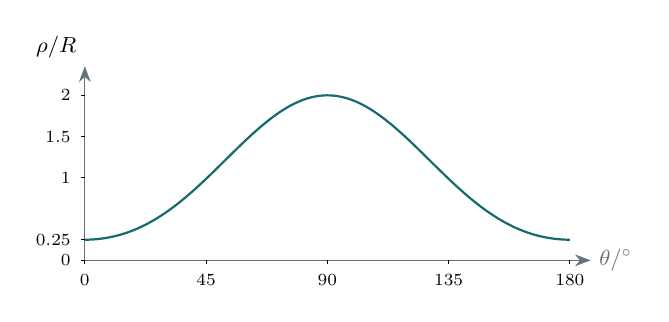
\begin{tikzpicture}[scale=.88,transform shape]
\draw[axis] (0,0.0)--(7.3,0.0) node[right] {$\theta/{}^\circ$};
\draw[axis] (0,0)--(0,2.8);
\node[above left] at (0,2.8) {$\rho/R$};
\draw[thin] (0.000000,0.0)--(0.000000,-0.06);\node[below,font=\scriptsize] at (0.000000,-0.08) {$ 0 $};
\draw[thin] (1.750000,0.0)--(1.750000,-0.06);\node[below,font=\scriptsize] at (1.750000,-0.08) {$ 45 $};
\draw[thin] (3.500000,0.0)--(3.500000,-0.06);\node[below,font=\scriptsize] at (3.500000,-0.08) {$ 90 $};
\draw[thin] (5.250000,0.0)--(5.250000,-0.06);\node[below,font=\scriptsize] at (5.250000,-0.08) {$ 135 $};
\draw[thin] (7.000000,0.0)--(7.000000,-0.06);\node[below,font=\scriptsize] at (7.000000,-0.08) {$ 180 $};
\draw[thin] (0,0.000000)--(-.06,0.000000);\node[left,font=\scriptsize] at (-.08,0.000000) {$ 0 $};
\draw[thin] (0,0.297619)--(-.06,0.297619);\node[left,font=\scriptsize] at (-.08,0.297619) {$ 0.25 $};
\draw[thin] (0,1.190476)--(-.06,1.190476);\node[left,font=\scriptsize] at (-.08,1.190476) {$ 1 $};
\draw[thin] (0,1.785714)--(-.06,1.785714);\node[left,font=\scriptsize] at (-.08,1.785714) {$ 1.5 $};
\draw[thin] (0,2.380952)--(-.06,2.380952);\node[left,font=\scriptsize] at (-.08,2.380952) {$ 2 $};
\draw[thick,color=accent] plot coordinates {(0.0000000,0.2976190) (0.0291667,0.2978485) (0.0583333,0.2985372) (0.0875000,0.2996857) (0.1166667,0.3012949) (0.1458333,0.3033663) (0.1750000,0.3059014) (0.2041667,0.3089024) (0.2333333,0.3123716) (0.2625000,0.3163117) (0.2916667,0.3207257) (0.3208333,0.3256167) (0.3500000,0.3309881) (0.3791667,0.3368435) (0.4083333,0.3431865) (0.4375000,0.3500211) (0.4666667,0.3573509) (0.4958333,0.3651800) (0.5250000,0.3735122) (0.5541667,0.3823513) (0.5833333,0.3917009) (0.6125000,0.4015646) (0.6416667,0.4119458) (0.6708333,0.4228475) (0.7000000,0.4342727) (0.7291667,0.4462238) (0.7583333,0.4587031) (0.7875000,0.4717124) (0.8166667,0.4852532) (0.8458333,0.4993262) (0.8750000,0.5139321) (0.9041667,0.5290707) (0.9333333,0.5447416) (0.9625000,0.5609434) (0.9916667,0.5776746) (1.0208333,0.5949326) (1.0500000,0.6127145) (1.0791667,0.6310167) (1.1083333,0.6498348) (1.1375000,0.6691637) (1.1666667,0.6889977) (1.1958333,0.7093305) (1.2250000,0.7301547) (1.2541667,0.7514625) (1.2833333,0.7732452) (1.3125000,0.7954935) (1.3416667,0.8181972) (1.3708333,0.8413454) (1.4000000,0.8649265) (1.4291667,0.8889281) (1.4583333,0.9133371) (1.4875000,0.9381397) (1.5166667,0.9633212) (1.5458333,0.9888666) (1.5750000,1.0147597) (1.6041667,1.0409839) (1.6333333,1.0675219) (1.6625000,1.0943557) (1.6916667,1.1214667) (1.7208333,1.1488356) (1.7500000,1.1764426) (1.7791667,1.2042672) (1.8083333,1.2322886) (1.8375000,1.2604851) (1.8666667,1.2888347) (1.8958333,1.3173150) (1.9250000,1.3459030) (1.9541667,1.3745752) (1.9833333,1.4033080) (2.0125000,1.4320772) (2.0416667,1.4608582) (2.0708333,1.4896263) (2.1000000,1.5183564) (2.1291667,1.5470232) (2.1583333,1.5756011) (2.1875000,1.6040646) (2.2166667,1.6323876) (2.2458333,1.6605443) (2.2750000,1.6885087) (2.3041667,1.7162547) (2.3333333,1.7437562) (2.3625000,1.7709872) (2.3916667,1.7979218) (2.4208333,1.8245340) (2.4500000,1.8507982) (2.4791667,1.8766889) (2.5083333,1.9021807) (2.5375000,1.9272485) (2.5666667,1.9518675) (2.5958333,1.9760133) (2.6250000,1.9996616) (2.6541667,2.0227888) (2.6833333,2.0453716) (2.7125000,2.0673870) (2.7416667,2.0888126) (2.7708333,2.1096265) (2.8000000,2.1298074) (2.8291667,2.1493346) (2.8583333,2.1681878) (2.8875000,2.1863476) (2.9166667,2.2037950) (2.9458333,2.2205119) (2.9750000,2.2364809) (3.0041667,2.2516851) (3.0333333,2.2661087) (3.0625000,2.2797363) (3.0916667,2.2925538) (3.1208333,2.3045475) (3.1500000,2.3157048) (3.1791667,2.3260137) (3.2083333,2.3354634) (3.2375000,2.3440438) (3.2666667,2.3517458) (3.2958333,2.3585612) (3.3250000,2.3644826) (3.3541667,2.3695038) (3.3833333,2.3736194) (3.4125000,2.3768250) (3.4416667,2.3791172) (3.4708333,2.3804935) (3.5000000,2.3809524) (3.5291667,2.3804935) (3.5583333,2.3791172) (3.5875000,2.3768250) (3.6166667,2.3736194) (3.6458333,2.3695038) (3.6750000,2.3644826) (3.7041667,2.3585612) (3.7333333,2.3517458) (3.7625000,2.3440438) (3.7916667,2.3354634) (3.8208333,2.3260137) (3.8500000,2.3157048) (3.8791667,2.3045475) (3.9083333,2.2925538) (3.9375000,2.2797363) (3.9666667,2.2661087) (3.9958333,2.2516851) (4.0250000,2.2364809) (4.0541667,2.2205119) (4.0833333,2.2037950) (4.1125000,2.1863476) (4.1416667,2.1681878) (4.1708333,2.1493346) (4.2000000,2.1298074) (4.2291667,2.1096265) (4.2583333,2.0888126) (4.2875000,2.0673870) (4.3166667,2.0453716) (4.3458333,2.0227888) (4.3750000,1.9996616) (4.4041667,1.9760133) (4.4333333,1.9518675) (4.4625000,1.9272485) (4.4916667,1.9021807) (4.5208333,1.8766889) (4.5500000,1.8507982) (4.5791667,1.8245340) (4.6083333,1.7979218) (4.6375000,1.7709872) (4.6666667,1.7437562) (4.6958333,1.7162547) (4.7250000,1.6885087) (4.7541667,1.6605443) (4.7833333,1.6323876) (4.8125000,1.6040646) (4.8416667,1.5756011) (4.8708333,1.5470232) (4.9000000,1.5183564) (4.9291667,1.4896263) (4.9583333,1.4608582) (4.9875000,1.4320772) (5.0166667,1.4033080) (5.0458333,1.3745752) (5.0750000,1.3459030) (5.1041667,1.3173150) (5.1333333,1.2888347) (5.1625000,1.2604851) (5.1916667,1.2322886) (5.2208333,1.2042672) (5.2500000,1.1764426) (5.2791667,1.1488356) (5.3083333,1.1214667) (5.3375000,1.0943557) (5.3666667,1.0675219) (5.3958333,1.0409839) (5.4250000,1.0147597) (5.4541667,0.9888666) (5.4833333,0.9633212) (5.5125000,0.9381397) (5.5416667,0.9133371) (5.5708333,0.8889281) (5.6000000,0.8649265) (5.6291667,0.8413454) (5.6583333,0.8181972) (5.6875000,0.7954935) (5.7166667,0.7732452) (5.7458333,0.7514625) (5.7750000,0.7301547) (5.8041667,0.7093305) (5.8333333,0.6889977) (5.8625000,0.6691637) (5.8916667,0.6498348) (5.9208333,0.6310167) (5.9500000,0.6127145) (5.9791667,0.5949326) (6.0083333,0.5776746) (6.0375000,0.5609434) (6.0666667,0.5447416) (6.0958333,0.5290707) (6.1250000,0.5139321) (6.1541667,0.4993262) (6.1833333,0.4852532) (6.2125000,0.4717124) (6.2416667,0.4587031) (6.2708333,0.4462238) (6.3000000,0.4342727) (6.3291667,0.4228475) (6.3583333,0.4119458) (6.3875000,0.4015646) (6.4166667,0.3917009) (6.4458333,0.3823513) (6.4750000,0.3735122) (6.5041667,0.3651800) (6.5333333,0.3573509) (6.5625000,0.3500211) (6.5916667,0.3431865) (6.6208333,0.3368435) (6.6500000,0.3309881) (6.6791667,0.3256167) (6.7083333,0.3207257) (6.7375000,0.3163117) (6.7666667,0.3123716) (6.7958333,0.3089024) (6.8250000,0.3059014) (6.8541667,0.3033663) (6.8833333,0.3012949) (6.9125000,0.2996857) (6.9416667,0.2985372) (6.9708333,0.2978485) (7.0000000,0.2976190)};
\end{tikzpicture}
\figcaption{变图力试1.2V6\quad 任意位置曲率的导数决定右端与底部的极值}
\end{minipage}\end{center}
\item \textbf{从较低位置静止释放。}开始时环心在$O$，球在$0<\theta_0<\pi$处与环均静止，求轨迹和下滑速率。

令$\eta=1-k=m/(M+m)$。积分常量变为$mx+MX=mR\sin\theta_0$，故
\[
 x=kR\sin\theta+(1-k)R\sin\theta_0,\quad y=R\cos\theta,
 \qquad
 \dot\theta^2=\frac{2g(\cos\theta_0-\cos\theta)}
 {R(1-\eta\cos^2\theta)}.
\]
地面椭圆水平平移$(1-k)R\sin\theta_0$，两半轴和几何曲率保持。变图力试1.2V7取$k=1/2,\theta_0=30^\circ$，从释放角的零速率下滑到B。该轨迹的实际运动段由$\cos\theta\le\cos\theta_0$给出。
\begin{center}\begin{minipage}{.98\linewidth}\centering
\begin{tikzpicture}[scale=.88,transform shape]
\draw[axis] (0,0.0)--(7.3,0.0) node[right] {$\theta/{}^\circ$};
\draw[axis] (0,0)--(0,2.8);
\node[above left] at (0,2.8) {$R\dot\theta^2/g$};
\draw[thin] (0.000000,0.0)--(0.000000,-0.06);\node[below,font=\scriptsize] at (0.000000,-0.08) {$ 30 $};
\draw[thin] (1.400000,0.0)--(1.400000,-0.06);\node[below,font=\scriptsize] at (1.400000,-0.08) {$ 60 $};
\draw[thin] (2.800000,0.0)--(2.800000,-0.06);\node[below,font=\scriptsize] at (2.800000,-0.08) {$ 90 $};
\draw[thin] (4.200000,0.0)--(4.200000,-0.06);\node[below,font=\scriptsize] at (4.200000,-0.08) {$ 120 $};
\draw[thin] (5.600000,0.0)--(5.600000,-0.06);\node[below,font=\scriptsize] at (5.600000,-0.08) {$ 150 $};
\draw[thin] (7.000000,0.0)--(7.000000,-0.06);\node[below,font=\scriptsize] at (7.000000,-0.08) {$ 180 $};
\draw[thin] (0,0.000000)--(-.06,0.000000);\node[left,font=\scriptsize] at (-.08,0.000000) {$ 0 $};
\draw[thin] (0,0.641026)--(-.06,0.641026);\node[left,font=\scriptsize] at (-.08,0.641026) {$ 2 $};
\draw[thin] (0,1.282051)--(-.06,1.282051);\node[left,font=\scriptsize] at (-.08,1.282051) {$ 4 $};
\draw[thin] (0,1.923077)--(-.06,1.923077);\node[left,font=\scriptsize] at (-.08,1.923077) {$ 6 $};
\draw[thick,color=accent] plot coordinates {(0.0000000,0.0000000) (0.0291667,0.0056041) (0.0583333,0.0112267) (0.0875000,0.0168653) (0.1166667,0.0225173) (0.1458333,0.0281807) (0.1750000,0.0338532) (0.2041667,0.0395329) (0.2333333,0.0452178) (0.2625000,0.0509063) (0.2916667,0.0565968) (0.3208333,0.0622876) (0.3500000,0.0679775) (0.3791667,0.0736652) (0.4083333,0.0793495) (0.4375000,0.0850294) (0.4666667,0.0907040) (0.4958333,0.0963724) (0.5250000,0.1020339) (0.5541667,0.1076878) (0.5833333,0.1133336) (0.6125000,0.1189709) (0.6416667,0.1245992) (0.6708333,0.1302183) (0.7000000,0.1358279) (0.7291667,0.1414279) (0.7583333,0.1470182) (0.7875000,0.1525989) (0.8166667,0.1581700) (0.8458333,0.1637316) (0.8750000,0.1692839) (0.9041667,0.1748272) (0.9333333,0.1803617) (0.9625000,0.1858879) (0.9916667,0.1914060) (1.0208333,0.1969167) (1.0500000,0.2024203) (1.0791667,0.2079175) (1.1083333,0.2134087) (1.1375000,0.2188947) (1.1666667,0.2243760) (1.1958333,0.2298534) (1.2250000,0.2353276) (1.2541667,0.2407994) (1.2833333,0.2462695) (1.3125000,0.2517389) (1.3416667,0.2572082) (1.3708333,0.2626784) (1.4000000,0.2681505) (1.4291667,0.2736253) (1.4583333,0.2791037) (1.4875000,0.2845868) (1.5166667,0.2900756) (1.5458333,0.2955710) (1.5750000,0.3010740) (1.6041667,0.3065859) (1.6333333,0.3121075) (1.6625000,0.3176401) (1.6916667,0.3231846) (1.7208333,0.3287423) (1.7500000,0.3343142) (1.7791667,0.3399015) (1.8083333,0.3455054) (1.8375000,0.3511271) (1.8666667,0.3567678) (1.8958333,0.3624286) (1.9250000,0.3681108) (1.9541667,0.3738156) (1.9833333,0.3795443) (2.0125000,0.3852982) (2.0416667,0.3910785) (2.0708333,0.3968865) (2.1000000,0.4027235) (2.1291667,0.4085909) (2.1583333,0.4144900) (2.1875000,0.4204220) (2.2166667,0.4263885) (2.2458333,0.4323907) (2.2750000,0.4384300) (2.3041667,0.4445078) (2.3333333,0.4506256) (2.3625000,0.4567847) (2.3916667,0.4629866) (2.4208333,0.4692328) (2.4500000,0.4755246) (2.4791667,0.4818637) (2.5083333,0.4882514) (2.5375000,0.4946893) (2.5666667,0.5011789) (2.5958333,0.5077218) (2.6250000,0.5143194) (2.6541667,0.5209734) (2.6833333,0.5276853) (2.7125000,0.5344568) (2.7416667,0.5412894) (2.7708333,0.5481847) (2.8000000,0.5551445) (2.8291667,0.5621703) (2.8583333,0.5692638) (2.8875000,0.5764268) (2.9166667,0.5836609) (2.9458333,0.5909678) (2.9750000,0.5983493) (3.0041667,0.6058071) (3.0333333,0.6133431) (3.0625000,0.6209589) (3.0916667,0.6286564) (3.1208333,0.6364373) (3.1500000,0.6443037) (3.1791667,0.6522571) (3.2083333,0.6602997) (3.2375000,0.6684331) (3.2666667,0.6766593) (3.2958333,0.6849803) (3.3250000,0.6933978) (3.3541667,0.7019140) (3.3833333,0.7105306) (3.4125000,0.7192498) (3.4416667,0.7280733) (3.4708333,0.7370034) (3.5000000,0.7460418) (3.5291667,0.7551907) (3.5583333,0.7644520) (3.5875000,0.7738278) (3.6166667,0.7833201) (3.6458333,0.7929309) (3.6750000,0.8026623) (3.7041667,0.8125163) (3.7333333,0.8224950) (3.7625000,0.8326004) (3.7916667,0.8428345) (3.8208333,0.8531994) (3.8500000,0.8636971) (3.8791667,0.8743297) (3.9083333,0.8850992) (3.9375000,0.8960074) (3.9666667,0.9070566) (3.9958333,0.9182486) (4.0250000,0.9295853) (4.0541667,0.9410687) (4.0833333,0.9527007) (4.1125000,0.9644831) (4.1416667,0.9764179) (4.1708333,0.9885066) (4.2000000,1.0007512) (4.2291667,1.0131533) (4.2583333,1.0257145) (4.2875000,1.0384365) (4.3166667,1.0513207) (4.3458333,1.0643685) (4.3750000,1.0775815) (4.4041667,1.0909608) (4.4333333,1.1045076) (4.4625000,1.1182232) (4.4916667,1.1321083) (4.5208333,1.1461641) (4.5500000,1.1603911) (4.5791667,1.1747902) (4.6083333,1.1893617) (4.6375000,1.2041060) (4.6666667,1.2190234) (4.6958333,1.2341138) (4.7250000,1.2493773) (4.7541667,1.2648133) (4.7833333,1.2804215) (4.8125000,1.2962010) (4.8416667,1.3121510) (4.8708333,1.3282703) (4.9000000,1.3445574) (4.9291667,1.3610107) (4.9583333,1.3776282) (4.9875000,1.3944076) (5.0166667,1.4113465) (5.0458333,1.4284420) (5.0750000,1.4456910) (5.1041667,1.4630898) (5.1333333,1.4806347) (5.1625000,1.4983213) (5.1916667,1.5161452) (5.2208333,1.5341013) (5.2500000,1.5521840) (5.2791667,1.5703877) (5.3083333,1.5887059) (5.3375000,1.6071320) (5.3666667,1.6256586) (5.3958333,1.6442781) (5.4250000,1.6629824) (5.4541667,1.6817626) (5.4833333,1.7006096) (5.5125000,1.7195136) (5.5416667,1.7384644) (5.5708333,1.7574511) (5.6000000,1.7764624) (5.6291667,1.7954863) (5.6583333,1.8145103) (5.6875000,1.8335215) (5.7166667,1.8525062) (5.7458333,1.8714503) (5.7750000,1.8903391) (5.8041667,1.9091572) (5.8333333,1.9278891) (5.8625000,1.9465183) (5.8916667,1.9650281) (5.9208333,1.9834011) (5.9500000,2.0016195) (5.9791667,2.0196652) (6.0083333,2.0375196) (6.0375000,2.0551635) (6.0666667,2.0725776) (6.0958333,2.0897422) (6.1250000,2.1066372) (6.1541667,2.1232425) (6.1833333,2.1395375) (6.2125000,2.1555018) (6.2416667,2.1711146) (6.2708333,2.1863551) (6.3000000,2.2012028) (6.3291667,2.2156369) (6.3583333,2.2296369) (6.3875000,2.2431826) (6.4166667,2.2562538) (6.4458333,2.2688309) (6.4750000,2.2808946) (6.5041667,2.2924260) (6.5333333,2.3034068) (6.5625000,2.3138193) (6.5916667,2.3236464) (6.6208333,2.3328719) (6.6500000,2.3414801) (6.6791667,2.3494566) (6.7083333,2.3567875) (6.7375000,2.3634602) (6.7666667,2.3694629) (6.7958333,2.3747851) (6.8250000,2.3794172) (6.8541667,2.3833509) (6.8833333,2.3865792) (6.9125000,2.3890962) (6.9416667,2.3908974) (6.9708333,2.3919794) (7.0000000,2.3923403)};
\end{tikzpicture}
\figcaption{变图力试1.2V7\quad 从30度静止释放后的相对角速率}
\end{minipage}\end{center}
\item \textbf{小扰动的下滑时间。}球从小角度$\theta_0>0$静止释放，求到达另一个小角度$\theta_1>\theta_0$的时间近似。

小角度时有效动能为$\tfrac12mkR^2\dot\theta^2$，重力势能在顶端为$mgR-\tfrac12mgR\theta^2$，运动方程线性化为$kR\ddot\theta=g\theta$。初值解为
\[
 \theta=\theta_0\cosh\left(\sqrt{\frac g{kR}}\,t\right),\qquad
 t_1=\sqrt{\frac{kR}g}\operatorname{arcosh}\frac{\theta_1}{\theta_0}.
\]
变图力试1.2V8画无量纲时间随$\theta_0/\theta_1$的变化。若$\theta_0\ll\theta_1$，$t_1\simeq\sqrt{kR/g}\ln(2\theta_1/\theta_0)$，扰动趋零使离开最高点的时间按对数增长；空间椭圆及其曲率仍保持相同极限。
\begin{center}\begin{minipage}{.98\linewidth}\centering
\begin{tikzpicture}[scale=.88,transform shape]
\draw[axis] (0,0.0)--(7.3,0.0) node[right] {$\theta_0/\theta_1$};
\draw[axis] (0,0)--(0,2.8);
\node[above left] at (0,2.8) {$t_1\sqrt{g/(kR)}$};
\draw[thin] (0.000000,0.0)--(0.000000,-0.06);\node[below,font=\scriptsize] at (0.000000,-0.08) {$ 0.01 $};
\draw[thin] (1.285714,0.0)--(1.285714,-0.06);\node[below,font=\scriptsize] at (1.285714,-0.08) {$ 0.1 $};
\draw[thin] (2.714286,0.0)--(2.714286,-0.06);\node[below,font=\scriptsize] at (2.714286,-0.08) {$ 0.2 $};
\draw[thin] (4.142857,0.0)--(4.142857,-0.06);\node[below,font=\scriptsize] at (4.142857,-0.08) {$ 0.3 $};
\draw[thin] (5.571429,0.0)--(5.571429,-0.06);\node[below,font=\scriptsize] at (5.571429,-0.08) {$ 0.4 $};
\draw[thin] (7.000000,0.0)--(7.000000,-0.06);\node[below,font=\scriptsize] at (7.000000,-0.08) {$ 0.5 $};
\draw[thin] (0,0.000000)--(-.06,0.000000);\node[left,font=\scriptsize] at (-.08,0.000000) {$ 0 $};
\draw[thin] (0,0.454545)--(-.06,0.454545);\node[left,font=\scriptsize] at (-.08,0.454545) {$ 1 $};
\draw[thin] (0,0.909091)--(-.06,0.909091);\node[left,font=\scriptsize] at (-.08,0.909091) {$ 2 $};
\draw[thin] (0,1.363636)--(-.06,1.363636);\node[left,font=\scriptsize] at (-.08,1.363636) {$ 3 $};
\draw[thin] (0,1.818182)--(-.06,1.818182);\node[left,font=\scriptsize] at (-.08,1.818182) {$ 4 $};
\draw[thin] (0,2.272727)--(-.06,2.272727);\node[left,font=\scriptsize] at (-.08,2.272727) {$ 5 $};
\draw[thick,color=accent] plot coordinates {(0.0000000,2.4083147) (0.0291667,2.3238606) (0.0583333,2.2526640) (0.0875000,2.1911212) (0.1166667,2.1369234) (0.1458333,2.0885024) (0.1750000,2.0447439) (0.2041667,2.0048280) (0.2333333,1.9681334) (0.2625000,1.9341785) (0.2916667,1.9025820) (0.3208333,1.8730372) (0.3500000,1.8452934) (0.3791667,1.8191433) (0.4083333,1.7944135) (0.4375000,1.7709573) (0.4666667,1.7486496) (0.4958333,1.7273829) (0.5250000,1.7070643) (0.5541667,1.6876124) (0.5833333,1.6689561) (0.6125000,1.6510328) (0.6416667,1.6337867) (0.6708333,1.6171684) (0.7000000,1.6011335) (0.7291667,1.5856422) (0.7583333,1.5706589) (0.7875000,1.5561509) (0.8166667,1.5420889) (0.8458333,1.5284462) (0.8750000,1.5151982) (0.9041667,1.5023227) (0.9333333,1.4897991) (0.9625000,1.4776085) (0.9916667,1.4657335) (1.0208333,1.4541581) (1.0500000,1.4428674) (1.0791667,1.4318475) (1.1083333,1.4210857) (1.1375000,1.4105700) (1.1666667,1.4002892) (1.1958333,1.3902331) (1.2250000,1.3803918) (1.2541667,1.3707562) (1.2833333,1.3613179) (1.3125000,1.3520687) (1.3416667,1.3430011) (1.3708333,1.3341081) (1.4000000,1.3253829) (1.4291667,1.3168192) (1.4583333,1.3084110) (1.4875000,1.3001527) (1.5166667,1.2920389) (1.5458333,1.2840646) (1.5750000,1.2762249) (1.6041667,1.2685153) (1.6333333,1.2609314) (1.6625000,1.2534691) (1.6916667,1.2461245) (1.7208333,1.2388938) (1.7500000,1.2317734) (1.7791667,1.2247601) (1.8083333,1.2178504) (1.8375000,1.2110413) (1.8666667,1.2043298) (1.8958333,1.1977131) (1.9250000,1.1911884) (1.9541667,1.1847532) (1.9833333,1.1784050) (2.0125000,1.1721413) (2.0416667,1.1659598) (2.0708333,1.1598584) (2.1000000,1.1538348) (2.1291667,1.1478872) (2.1583333,1.1420135) (2.1875000,1.1362118) (2.2166667,1.1304802) (2.2458333,1.1248172) (2.2750000,1.1192209) (2.3041667,1.1136897) (2.3333333,1.1082222) (2.3625000,1.1028166) (2.3916667,1.0974717) (2.4208333,1.0921859) (2.4500000,1.0869580) (2.4791667,1.0817866) (2.5083333,1.0766703) (2.5375000,1.0716081) (2.5666667,1.0665987) (2.5958333,1.0616409) (2.6250000,1.0567337) (2.6541667,1.0518759) (2.6833333,1.0470665) (2.7125000,1.0423044) (2.7416667,1.0375888) (2.7708333,1.0329186) (2.8000000,1.0282929) (2.8291667,1.0237108) (2.8583333,1.0191715) (2.8875000,1.0146740) (2.9166667,1.0102176) (2.9458333,1.0058014) (2.9750000,1.0014248) (3.0041667,0.9970868) (3.0333333,0.9927869) (3.0625000,0.9885242) (3.0916667,0.9842981) (3.1208333,0.9801078) (3.1500000,0.9759529) (3.1791667,0.9718325) (3.2083333,0.9677461) (3.2375000,0.9636930) (3.2666667,0.9596727) (3.2958333,0.9556846) (3.3250000,0.9517281) (3.3541667,0.9478027) (3.3833333,0.9439078) (3.4125000,0.9400429) (3.4416667,0.9362076) (3.4708333,0.9324012) (3.5000000,0.9286233) (3.5291667,0.9248735) (3.5583333,0.9211513) (3.5875000,0.9174561) (3.6166667,0.9137877) (3.6458333,0.9101455) (3.6750000,0.9065291) (3.7041667,0.9029382) (3.7333333,0.8993723) (3.7625000,0.8958309) (3.7916667,0.8923138) (3.8208333,0.8888206) (3.8500000,0.8853508) (3.8791667,0.8819042) (3.9083333,0.8784803) (3.9375000,0.8750788) (3.9666667,0.8716995) (3.9958333,0.8683418) (4.0250000,0.8650056) (4.0541667,0.8616906) (4.0833333,0.8583963) (4.1125000,0.8551225) (4.1416667,0.8518688) (4.1708333,0.8486351) (4.2000000,0.8454210) (4.2291667,0.8422263) (4.2583333,0.8390506) (4.2875000,0.8358936) (4.3166667,0.8327552) (4.3458333,0.8296350) (4.3750000,0.8265329) (4.4041667,0.8234485) (4.4333333,0.8203816) (4.4625000,0.8173319) (4.4916667,0.8142993) (4.5208333,0.8112835) (4.5500000,0.8082843) (4.5791667,0.8053013) (4.6083333,0.8023346) (4.6375000,0.7993837) (4.6666667,0.7964485) (4.6958333,0.7935288) (4.7250000,0.7906243) (4.7541667,0.7877350) (4.7833333,0.7848605) (4.8125000,0.7820007) (4.8416667,0.7791554) (4.8708333,0.7763244) (4.9000000,0.7735076) (4.9291667,0.7707046) (4.9583333,0.7679155) (4.9875000,0.7651399) (5.0166667,0.7623777) (5.0458333,0.7596287) (5.0750000,0.7568929) (5.1041667,0.7541699) (5.1333333,0.7514597) (5.1625000,0.7487621) (5.1916667,0.7460769) (5.2208333,0.7434040) (5.2500000,0.7407432) (5.2791667,0.7380944) (5.3083333,0.7354574) (5.3375000,0.7328320) (5.3666667,0.7302182) (5.3958333,0.7276159) (5.4250000,0.7250247) (5.4541667,0.7224447) (5.4833333,0.7198757) (5.5125000,0.7173175) (5.5416667,0.7147700) (5.5708333,0.7122331) (5.6000000,0.7097067) (5.6291667,0.7071906) (5.6583333,0.7046848) (5.6875000,0.7021890) (5.7166667,0.6997032) (5.7458333,0.6972273) (5.7750000,0.6947610) (5.8041667,0.6923044) (5.8333333,0.6898573) (5.8625000,0.6874196) (5.8916667,0.6849912) (5.9208333,0.6825720) (5.9500000,0.6801618) (5.9791667,0.6777605) (6.0083333,0.6753681) (6.0375000,0.6729845) (6.0666667,0.6706095) (6.0958333,0.6682431) (6.1250000,0.6658850) (6.1541667,0.6635354) (6.1833333,0.6611940) (6.2125000,0.6588607) (6.2416667,0.6565354) (6.2708333,0.6542182) (6.3000000,0.6519088) (6.3291667,0.6496071) (6.3583333,0.6473132) (6.3875000,0.6450268) (6.4166667,0.6427480) (6.4458333,0.6404765) (6.4750000,0.6382124) (6.5041667,0.6359555) (6.5333333,0.6337058) (6.5625000,0.6314632) (6.5916667,0.6292275) (6.6208333,0.6269987) (6.6500000,0.6247768) (6.6791667,0.6225616) (6.7083333,0.6203531) (6.7375000,0.6181511) (6.7666667,0.6159557) (6.7958333,0.6137667) (6.8250000,0.6115840) (6.8541667,0.6094076) (6.8833333,0.6072374) (6.9125000,0.6050734) (6.9416667,0.6029154) (6.9708333,0.6007633) (7.0000000,0.5986172)};
\end{tikzpicture}
\figcaption{变图力试1.2V8\quad 小角度近似下扰动幅度与离顶所需时间}
\end{minipage}\end{center}
\end{enumerate}

\Needspace{13\baselineskip}

\pdfbookmark[2]{第 3 题 螺旋槽内下滑与圆筒的平移、自转}{q3}

\section*{第 3 题\quad 螺旋槽内下滑与圆筒的平移、自转}\label{q:3}


质量为$M$、半径为$R$的均匀薄壁圆筒竖直放在光滑水平面上，可水平平移并绕竖直轴自转，保持竖直而不倾倒。筒内壁有一条光滑螺旋槽，筒高$h$恰等于螺距，即沿槽绕筒一周恰从顶端到达底端。小球质量为$m$，从槽顶与圆筒一同静止开始下滑。
\begin{enumerate}
\item 说明下滑过程中圆筒轴线的水平运动与圆筒自转。
\item 求小球从槽顶到槽底相对地面走过的总路程。
\end{enumerate}
圆筒绕自身竖直轴的转动惯量为$I=MR^2$。忽略摩擦和小球尺寸。


\begin{center}\begin{minipage}{.98\linewidth}\centering
\begin{tikzpicture}[scale=.9,transform shape]
\draw[object] plot coordinates {(2.00000,0.00000) (1.99822,0.01897) (1.99289,0.03791) (1.98402,0.05678) (1.97162,0.07554) (1.95571,0.09418) (1.93632,0.11265) (1.91350,0.13091) (1.88727,0.14895) (1.85768,0.16671) (1.82480,0.18419) (1.78866,0.20133) (1.74935,0.21812) (1.70693,0.23452) (1.66147,0.25050) (1.61306,0.26604) (1.56178,0.28110) (1.50773,0.29566) (1.45099,0.30970) (1.39167,0.32319) (1.32988,0.33610) (1.26573,0.34842) (1.19932,0.36011) (1.13078,0.37117) (1.06024,0.38157) (0.98780,0.39128) (0.91361,0.40030) (0.83780,0.40861) (0.76049,0.41620) (0.68184,0.42304) (0.60197,0.42913) (0.52103,0.43446) (0.43917,0.43902) (0.35652,0.44279) (0.27324,0.44578) (0.18948,0.44798) (0.10537,0.44937) (0.02108,0.44997) (-0.06324,0.44977) (-0.14746,0.44878) (-0.23141,0.44698) (-0.31495,0.44439) (-0.39793,0.44100) (-0.48021,0.43684) (-0.56163,0.43189) (-0.64205,0.42618) (-0.72133,0.41971) (-0.79932,0.41250) (-0.87590,0.40455) (-0.95092,0.39588) (-1.02425,0.38651) (-1.09575,0.37645) (-1.16531,0.36572) (-1.23280,0.35435) (-1.29809,0.34234) (-1.36108,0.32972) (-1.42165,0.31652) (-1.47969,0.30275) (-1.53510,0.28845) (-1.58778,0.27363) (-1.63763,0.25833) (-1.68458,0.24256) (-1.72853,0.22637) (-1.76940,0.20977) (-1.80713,0.19280) (-1.84165,0.17549) (-1.87289,0.15786) (-1.90081,0.13996) (-1.92534,0.12181) (-1.94645,0.10344) (-1.96410,0.08488) (-1.97826,0.06618) (-1.98890,0.04735) (-1.99600,0.02845) (-1.99956,0.00949) (-1.99956,-0.00949) (-1.99600,-0.02845) (-1.98890,-0.04735) (-1.97826,-0.06618) (-1.96410,-0.08488) (-1.94645,-0.10344) (-1.92534,-0.12181) (-1.90081,-0.13996) (-1.87289,-0.15786) (-1.84165,-0.17549) (-1.80713,-0.19280) (-1.76940,-0.20977) (-1.72853,-0.22637) (-1.68458,-0.24256) (-1.63763,-0.25833) (-1.58778,-0.27363) (-1.53510,-0.28845) (-1.47969,-0.30275) (-1.42165,-0.31652) (-1.36108,-0.32972) (-1.29809,-0.34234) (-1.23280,-0.35435) (-1.16531,-0.36572) (-1.09575,-0.37645) (-1.02425,-0.38651) (-0.95092,-0.39588) (-0.87590,-0.40455) (-0.79932,-0.41250) (-0.72133,-0.41971) (-0.64205,-0.42618) (-0.56163,-0.43189) (-0.48021,-0.43684) (-0.39793,-0.44100) (-0.31495,-0.44439) (-0.23141,-0.44698) (-0.14746,-0.44878) (-0.06324,-0.44977) (0.02108,-0.44997) (0.10537,-0.44937) (0.18948,-0.44798) (0.27324,-0.44578) (0.35652,-0.44279) (0.43917,-0.43902) (0.52103,-0.43446) (0.60197,-0.42913) (0.68184,-0.42304) (0.76049,-0.41620) (0.83780,-0.40861) (0.91361,-0.40030) (0.98780,-0.39128) (1.06024,-0.38157) (1.13078,-0.37117) (1.19932,-0.36011) (1.26573,-0.34842) (1.32988,-0.33610) (1.39167,-0.32319) (1.45099,-0.30970) (1.50773,-0.29566) (1.56178,-0.28110) (1.61306,-0.26604) (1.66147,-0.25050) (1.70693,-0.23452) (1.74935,-0.21812) (1.78866,-0.20133) (1.82480,-0.18419) (1.85768,-0.16671) (1.88727,-0.14895) (1.91350,-0.13091) (1.93632,-0.11265) (1.95571,-0.09418) (1.97162,-0.07554) (1.98402,-0.05678) (1.99289,-0.03791) (1.99822,-0.01897) (2.00000,-0.00000)};\draw[object] plot coordinates {(2.00000,5.00000) (1.99822,5.01897) (1.99289,5.03791) (1.98402,5.05678) (1.97162,5.07554) (1.95571,5.09418) (1.93632,5.11265) (1.91350,5.13091) (1.88727,5.14895) (1.85768,5.16671) (1.82480,5.18419) (1.78866,5.20133) (1.74935,5.21812) (1.70693,5.23452) (1.66147,5.25050) (1.61306,5.26604) (1.56178,5.28110) (1.50773,5.29566) (1.45099,5.30970) (1.39167,5.32319) (1.32988,5.33610) (1.26573,5.34842) (1.19932,5.36011) (1.13078,5.37117) (1.06024,5.38157) (0.98780,5.39128) (0.91361,5.40030) (0.83780,5.40861) (0.76049,5.41620) (0.68184,5.42304) (0.60197,5.42913) (0.52103,5.43446) (0.43917,5.43902) (0.35652,5.44279) (0.27324,5.44578) (0.18948,5.44798) (0.10537,5.44937) (0.02108,5.44997) (-0.06324,5.44977) (-0.14746,5.44878) (-0.23141,5.44698) (-0.31495,5.44439) (-0.39793,5.44100) (-0.48021,5.43684) (-0.56163,5.43189) (-0.64205,5.42618) (-0.72133,5.41971) (-0.79932,5.41250) (-0.87590,5.40455) (-0.95092,5.39588) (-1.02425,5.38651) (-1.09575,5.37645) (-1.16531,5.36572) (-1.23280,5.35435) (-1.29809,5.34234) (-1.36108,5.32972) (-1.42165,5.31652) (-1.47969,5.30275) (-1.53510,5.28845) (-1.58778,5.27363) (-1.63763,5.25833) (-1.68458,5.24256) (-1.72853,5.22637) (-1.76940,5.20977) (-1.80713,5.19280) (-1.84165,5.17549) (-1.87289,5.15786) (-1.90081,5.13996) (-1.92534,5.12181) (-1.94645,5.10344) (-1.96410,5.08488) (-1.97826,5.06618) (-1.98890,5.04735) (-1.99600,5.02845) (-1.99956,5.00949) (-1.99956,4.99051) (-1.99600,4.97155) (-1.98890,4.95265) (-1.97826,4.93382) (-1.96410,4.91512) (-1.94645,4.89656) (-1.92534,4.87819) (-1.90081,4.86004) (-1.87289,4.84214) (-1.84165,4.82451) (-1.80713,4.80720) (-1.76940,4.79023) (-1.72853,4.77363) (-1.68458,4.75744) (-1.63763,4.74167) (-1.58778,4.72637) (-1.53510,4.71155) (-1.47969,4.69725) (-1.42165,4.68348) (-1.36108,4.67028) (-1.29809,4.65766) (-1.23280,4.64565) (-1.16531,4.63428) (-1.09575,4.62355) (-1.02425,4.61349) (-0.95092,4.60412) (-0.87590,4.59545) (-0.79932,4.58750) (-0.72133,4.58029) (-0.64205,4.57382) (-0.56163,4.56811) (-0.48021,4.56316) (-0.39793,4.55900) (-0.31495,4.55561) (-0.23141,4.55302) (-0.14746,4.55122) (-0.06324,4.55023) (0.02108,4.55003) (0.10537,4.55063) (0.18948,4.55202) (0.27324,4.55422) (0.35652,4.55721) (0.43917,4.56098) (0.52103,4.56554) (0.60197,4.57087) (0.68184,4.57696) (0.76049,4.58380) (0.83780,4.59139) (0.91361,4.59970) (0.98780,4.60872) (1.06024,4.61843) (1.13078,4.62883) (1.19932,4.63989) (1.26573,4.65158) (1.32988,4.66390) (1.39167,4.67681) (1.45099,4.69030) (1.50773,4.70434) (1.56178,4.71890) (1.61306,4.73396) (1.66147,4.74950) (1.70693,4.76548) (1.74935,4.78188) (1.78866,4.79867) (1.82480,4.81581) (1.85768,4.83329) (1.88727,4.85105) (1.91350,4.86909) (1.93632,4.88735) (1.95571,4.90582) (1.97162,4.92446) (1.98402,4.94322) (1.99289,4.96209) (1.99822,4.98103) (2.00000,5.00000)};\draw[object] (-2.00000,0.00000)--(-2.00000,5.00000);\draw[object] (2.00000,0.00000)--(2.00000,5.00000);\draw[traj] plot coordinates {(2.00000,5.00000) (1.99918,4.99008) (1.99671,4.98015) (1.99260,4.97019) (1.98684,4.96021) (1.97946,4.95018) (1.97044,4.94010) (1.95980,4.92995) (1.94755,4.91973) (1.93370,4.90943) (1.91825,4.89903) (1.90122,4.88853) (1.88263,4.87791) (1.86250,4.86717) (1.84082,4.85629) (1.81764,4.84527) (1.79295,4.83409) (1.76679,4.82275) (1.73918,4.81124) (1.71013,4.79954) (1.67968,4.78765) (1.64785,4.77556) (1.61465,4.76326) (1.58013,4.75075) (1.54431,4.73800) (1.50722,4.72502) (1.46889,4.71179) (1.42935,4.69832) (1.38863,4.68458) (1.34677,4.67058) (1.30380,4.65631) (1.25976,4.64175) (1.21468,4.62691) (1.16860,4.61177) (1.12156,4.59633) (1.07359,4.58058) (1.02474,4.56453) (0.97505,4.54815) (0.92456,4.53145) (0.87330,4.51442) (0.82133,4.49706) (0.76868,4.47936) (0.71540,4.46132) (0.66153,4.44294) (0.60711,4.42420) (0.55219,4.40511) (0.49682,4.38567) (0.44105,4.36586) (0.38490,4.34570) (0.32844,4.32517) (0.27172,4.30428) (0.21476,4.28301) (0.15763,4.26139) (0.10037,4.23939) (0.04303,4.21702) (-0.01435,4.19428) (-0.07171,4.17117) (-0.12902,4.14769) (-0.18622,4.12384) (-0.24326,4.09963) (-0.30011,4.07504) (-0.35671,4.05009) (-0.41302,4.02478) (-0.46898,3.99910) (-0.52456,3.97306) (-0.57971,3.94666) (-0.63438,3.91991) (-0.68853,3.89281) (-0.74211,3.86536) (-0.79509,3.83757) (-0.84740,3.80944) (-0.89902,3.78097) (-0.94990,3.75217) (-1.00000,3.72304) (-1.04927,3.69360) (-1.09769,3.66384) (-1.14519,3.63377) (-1.19176,3.60339) (-1.23734,3.57272) (-1.28191,3.54176) (-1.32542,3.51051) (-1.36784,3.47899) (-1.40913,3.44719) (-1.44927,3.41513) (-1.48821,3.38282) (-1.52592,3.35026) (-1.56238,3.31746) (-1.59756,3.28443) (-1.63142,3.25118) (-1.66393,3.21771) (-1.69508,3.18403) (-1.72483,3.15016) (-1.75317,3.11611) (-1.78006,3.08187) (-1.80548,3.04747) (-1.82942,3.01290) (-1.85185,2.97819) (-1.87276,2.94333) (-1.89212,2.90835) (-1.90993,2.87325) (-1.92617,2.83803) (-1.94082,2.80272) (-1.95388,2.76732) (-1.96532,2.73184) (-1.97515,2.69629) (-1.98335,2.66068) (-1.98993,2.62502) (-1.99486,2.58933) (-1.99815,2.55361) (-1.99979,2.51787) (-1.99979,2.48213) (-1.99815,2.44639) (-1.99486,2.41067) (-1.98993,2.37498) (-1.98335,2.33932) (-1.97515,2.30371) (-1.96532,2.26816) (-1.95388,2.23268) (-1.94082,2.19728) (-1.92617,2.16197) (-1.90993,2.12675) (-1.89212,2.09165) (-1.87276,2.05667) (-1.85185,2.02181) (-1.82942,1.98710) (-1.80548,1.95253) (-1.78006,1.91813) (-1.75317,1.88389) (-1.72483,1.84984) (-1.69508,1.81597) (-1.66393,1.78229) (-1.63142,1.74882) (-1.59756,1.71557) (-1.56238,1.68254) (-1.52592,1.64974) (-1.48821,1.61718) (-1.44927,1.58487) (-1.40913,1.55281) (-1.36784,1.52101) (-1.32542,1.48949) (-1.28191,1.45824) (-1.23734,1.42728) (-1.19176,1.39661) (-1.14519,1.36623) (-1.09769,1.33616) (-1.04927,1.30640) (-1.00000,1.27696) (-0.94990,1.24783) (-0.89902,1.21903) (-0.84740,1.19056) (-0.79509,1.16243) (-0.74211,1.13464) (-0.68853,1.10719) (-0.63438,1.08009) (-0.57971,1.05334) (-0.52456,1.02694) (-0.46898,1.00090) (-0.41302,0.97522) (-0.35671,0.94991) (-0.30011,0.92496) (-0.24326,0.90037) (-0.18622,0.87616) (-0.12902,0.85231) (-0.07171,0.82883) (-0.01435,0.80572) (0.04303,0.78298) (0.10037,0.76061) (0.15763,0.73861) (0.21476,0.71699) (0.27172,0.69572) (0.32844,0.67483) (0.38490,0.65430) (0.44105,0.63414) (0.49682,0.61433) (0.55219,0.59489) (0.60711,0.57580) (0.66153,0.55706) (0.71540,0.53868) (0.76868,0.52064) (0.82133,0.50294) (0.87330,0.48558) (0.92456,0.46855) (0.97505,0.45185) (1.02474,0.43547) (1.07359,0.41942) (1.12156,0.40367) (1.16860,0.38823) (1.21468,0.37309) (1.25976,0.35825) (1.30380,0.34369) (1.34677,0.32942) (1.38863,0.31542) (1.42935,0.30168) (1.46889,0.28821) (1.50722,0.27498) (1.54431,0.26200) (1.58013,0.24925) (1.61465,0.23674) (1.64785,0.22444) (1.67968,0.21235) (1.71013,0.20046) (1.73918,0.18876) (1.76679,0.17725) (1.79295,0.16591) (1.81764,0.15473) (1.84082,0.14371) (1.86250,0.13283) (1.88263,0.12209) (1.90122,0.11147) (1.91825,0.10097) (1.93370,0.09057) (1.94755,0.08027) (1.95980,0.07005) (1.97044,0.05990) (1.97946,0.04982) (1.98684,0.03979) (1.99260,0.02981) (1.99671,0.01985) (1.99918,0.00992) (2.00000,-0.00000)};\fill (2.00000,5.00000) circle(.035);\node[above right] at (2.00000,5.00000) {$m$};\draw[<->,thin,color=muted] (3.00000,0.00000)--(3.00000,5.00000);\node[right] at (3.00000,2.50000) {$h$};\draw[<->,thin,color=muted] (0.00000,-1.00000)--(2.00000,-1.00000);\node[below] at (1.00000,-1.00000) {$R$};\node[above] at (0.00000,6.00000) {薄壁圆筒 $M$；螺旋槽一周};
\end{tikzpicture}
\figcaption{图力试1.3\quad 可平移、自转的圆筒及固定在筒壁上的一周槽。}
\end{minipage}\end{center}

\Needspace{8\baselineskip}

\pdfbookmark[3]{题型定位}{q3-h0}

\subsection*{题型定位}

水平质心固定给球与筒轴的公转半径，竖直轴角动量守恒同时包括两项公转和筒自转。带符号角的相对关系确定地面螺旋，路程由恒定投影微元比例积分。

\Needspace{8\baselineskip}

\pdfbookmark[3]{知识点}{q3-h1}

\subsection*{知识点}

\begin{itemize}
\item 水平外力为零且初始总动量为零，系统水平质心C固定。
\item 球与筒轴的公转半径分别为$MR/(M+m)$、$mR/(M+m)$。
\item 总竖直轴角动量包含球公转、筒轴公转及筒自转三项。
\item 同一正向的角满足$\theta=\varphi+\psi$，筒自转对应负的$\psi$。
\item 地面三维弧长用$\dd s^2=(r_m\dd\theta)^2+\dd z^2$，等螺距给常比例。\end{itemize}

\Needspace{8\baselineskip}

\pdfbookmark[3]{物理图像}{q3-h2}

\subsection*{物理图像}

A图的C固定，O与P围绕C在相反的位置公转，筒另有反向自转。B图画三个带符号角随相对角的线性关系。C图显示相等质量时地面不足一周的下降螺旋，D图将同一轨迹展开成水平弧长与竖直落差组成的直线。

\Needspace{8\baselineskip}

\pdfbookmark[3]{解题入口}{q3-h3}

\subsection*{解题入口}

先在俯视图标C、O、P并写两个半径，再定义同向计量的相对角、筒自转角和地面角。把三项角动量相加为零，联立相对角关系求各角比例；最后以同一个相对角微元写水平、竖直位移。

\Needspace{8\baselineskip}

\pdfbookmark[3]{标准解法}{q3-h4}

\subsection*{标准解法}


图力试1.3的槽绕筒一周规定的是球对筒的相对角。以沿槽下滑的相对角为$\varphi$，圆筒绕自身竖直轴的自转角为$\psi$，球在固定地面方向上的方位角为$\theta$，三个角取同一正向并从零开始：
\[
\theta=\varphi+\psi,\qquad
z=h-\frac{h}{2\pi}\varphi,\quad 0\le\varphi\le2\pi.
\]
下滑使$\varphi$增加，$\psi$可为负。竖直位置由螺旋槽的恒定螺距给出，水平运动与圆筒的平移、自转一同确定。

解图力试1.3A用$C$表示系统水平质心，$O$表示筒轴投影，$P$表示球的水平投影。地面光滑，系统无水平外力，初始总水平动量为零，故$C$在地面固定。由两质量的水平质心关系与$OP=R$，
\[
r_m=CP=\frac{M}{M+m}R,\qquad
r_M=CO=\frac{m}{M+m}R.
\]
$O,C,P$始终共线，$C$位于两个质量投影之间，$CO+CP=R$。因此球的水平投影和筒轴分别沿半径$r_m$、$r_M$的圆弧运动，两位置矢量相反，但它们相对固定地面方向的公转角速度同为$\dot\theta$。圆筒除此之外还可绕自身轴转动。
\begin{center}\begin{minipage}{.98\linewidth}\centering
\begin{tikzpicture}[scale=1.6]
\draw[object] (-.5,0) circle(1);\draw[guide] (0,0) circle(.5);
\fill (-.5,0) circle(.025) node[below left] {$O$};\fill (0,0) circle(.025) node[above] {$C$};\fill (.5,0) circle(.025) node[below right] {$P$};
\draw[guide] (-.5,0)--(.5,0);
\draw[motion] (.5,0)--(.5,.5) node[right] {球公转};\draw[motion] (-.5,0)--(-.5,-.5) node[left] {轴公转};
\draw[force] (-.735,.086) arc(160:40:.25);\node[left] at (-1,.8) {筒反向自转};
\draw[<->,thin,color=muted] (-.5,-.75)--(0,-.75) node[midway,below] {$r_M$};
\draw[<->,thin,color=muted] (0,-1.05)--(.5,-1.05) node[midway,below] {$r_m$};
\end{tikzpicture}
\figcaption{解图力试1.3A\quad 相等质量示例的水平投影，C固定，O和P反向分居两侧}
\end{minipage}\end{center}
关于过$C$的竖直轴，重力及地面竖直支持力的力矩在该轴上的分量均为零，球与筒之间的力属于内力，所以总竖直轴角动量保持初值零。球的公转、筒轴的公转以及筒自身的自转分别给
\[
\left(mr_m^2+Mr_M^2\right)\dot\theta+I\dot\psi=0.
\]
其中$\mu=Mm/(M+m)$，有$mr_m^2+Mr_M^2=\mu R^2$。两项公转都进入总角动量。代入$I=MR^2$及$\dot\theta=\dot\varphi+\dot\psi$，整理得
\[
\dot\theta=\frac{M+m}{M+2m}\dot\varphi,\qquad
\dot\psi=-\frac{m}{M+2m}\dot\varphi.
\]
把相同常比例从初始零角积分，
\[
\boxed{\theta=\frac{M+m}{M+2m}\varphi,\qquad
\psi=-\frac{m}{M+2m}\varphi}.
\]
解图力试1.3B画这三个带符号角随$\varphi$的关系：球与筒轴向同一方向公转，筒自转反向，三个角在每一时刻满足$\theta=\varphi+\psi$。
\begin{center}\begin{minipage}{.98\linewidth}\centering
\begin{tikzpicture}[scale=.88,transform shape]
\draw[axis] (0,0.6666666666666666)--(7.3,0.6666666666666666) node[right] {$\varphi/(2\pi)$};
\draw[axis] (0,0)--(0,2.8);
\node[above left] at (0,2.8) {$\text{带符号角}/(2\pi)$};
\draw[thin] (0.000000,0.6666666666666666)--(0.000000,0.6066666666666667);\node[below,font=\scriptsize] at (0.000000,0.5866666666666667) {$ 0 $};
\draw[thin] (1.750000,0.6666666666666666)--(1.750000,0.6066666666666667);\node[below,font=\scriptsize] at (1.750000,0.5866666666666667) {$ 0.25 $};
\draw[thin] (3.500000,0.6666666666666666)--(3.500000,0.6066666666666667);\node[below,font=\scriptsize] at (3.500000,0.5866666666666667) {$ 0.5 $};
\draw[thin] (5.250000,0.6666666666666666)--(5.250000,0.6066666666666667);\node[below,font=\scriptsize] at (5.250000,0.5866666666666667) {$ 0.75 $};
\draw[thin] (7.000000,0.6666666666666666)--(7.000000,0.6066666666666667);\node[below,font=\scriptsize] at (7.000000,0.5866666666666667) {$ 1 $};
\draw[thin] (0,0.111111)--(-.06,0.111111);\node[left,font=\scriptsize] at (-.08,0.111111) {$ -1/3 $};
\draw[thin] (0,0.666667)--(-.06,0.666667);\node[left,font=\scriptsize] at (-.08,0.666667) {$ 0 $};
\draw[thin] (0,1.222222)--(-.06,1.222222);\node[left,font=\scriptsize] at (-.08,1.222222) {$ 1/3 $};
\draw[thin] (0,1.777778)--(-.06,1.777778);\node[left,font=\scriptsize] at (-.08,1.777778) {$ 2/3 $};
\draw[thin] (0,2.333333)--(-.06,2.333333);\node[left,font=\scriptsize] at (-.08,2.333333) {$ 1 $};
\draw[thick,color=accent] plot coordinates {(0.0000000,0.6666667) (0.0291667,0.6712963) (0.0583333,0.6759259) (0.0875000,0.6805556) (0.1166667,0.6851852) (0.1458333,0.6898148) (0.1750000,0.6944444) (0.2041667,0.6990741) (0.2333333,0.7037037) (0.2625000,0.7083333) (0.2916667,0.7129630) (0.3208333,0.7175926) (0.3500000,0.7222222) (0.3791667,0.7268519) (0.4083333,0.7314815) (0.4375000,0.7361111) (0.4666667,0.7407407) (0.4958333,0.7453704) (0.5250000,0.7500000) (0.5541667,0.7546296) (0.5833333,0.7592593) (0.6125000,0.7638889) (0.6416667,0.7685185) (0.6708333,0.7731481) (0.7000000,0.7777778) (0.7291667,0.7824074) (0.7583333,0.7870370) (0.7875000,0.7916667) (0.8166667,0.7962963) (0.8458333,0.8009259) (0.8750000,0.8055556) (0.9041667,0.8101852) (0.9333333,0.8148148) (0.9625000,0.8194444) (0.9916667,0.8240741) (1.0208333,0.8287037) (1.0500000,0.8333333) (1.0791667,0.8379630) (1.1083333,0.8425926) (1.1375000,0.8472222) (1.1666667,0.8518519) (1.1958333,0.8564815) (1.2250000,0.8611111) (1.2541667,0.8657407) (1.2833333,0.8703704) (1.3125000,0.8750000) (1.3416667,0.8796296) (1.3708333,0.8842593) (1.4000000,0.8888889) (1.4291667,0.8935185) (1.4583333,0.8981481) (1.4875000,0.9027778) (1.5166667,0.9074074) (1.5458333,0.9120370) (1.5750000,0.9166667) (1.6041667,0.9212963) (1.6333333,0.9259259) (1.6625000,0.9305556) (1.6916667,0.9351852) (1.7208333,0.9398148) (1.7500000,0.9444444) (1.7791667,0.9490741) (1.8083333,0.9537037) (1.8375000,0.9583333) (1.8666667,0.9629630) (1.8958333,0.9675926) (1.9250000,0.9722222) (1.9541667,0.9768519) (1.9833333,0.9814815) (2.0125000,0.9861111) (2.0416667,0.9907407) (2.0708333,0.9953704) (2.1000000,1.0000000) (2.1291667,1.0046296) (2.1583333,1.0092593) (2.1875000,1.0138889) (2.2166667,1.0185185) (2.2458333,1.0231481) (2.2750000,1.0277778) (2.3041667,1.0324074) (2.3333333,1.0370370) (2.3625000,1.0416667) (2.3916667,1.0462963) (2.4208333,1.0509259) (2.4500000,1.0555556) (2.4791667,1.0601852) (2.5083333,1.0648148) (2.5375000,1.0694444) (2.5666667,1.0740741) (2.5958333,1.0787037) (2.6250000,1.0833333) (2.6541667,1.0879630) (2.6833333,1.0925926) (2.7125000,1.0972222) (2.7416667,1.1018519) (2.7708333,1.1064815) (2.8000000,1.1111111) (2.8291667,1.1157407) (2.8583333,1.1203704) (2.8875000,1.1250000) (2.9166667,1.1296296) (2.9458333,1.1342593) (2.9750000,1.1388889) (3.0041667,1.1435185) (3.0333333,1.1481481) (3.0625000,1.1527778) (3.0916667,1.1574074) (3.1208333,1.1620370) (3.1500000,1.1666667) (3.1791667,1.1712963) (3.2083333,1.1759259) (3.2375000,1.1805556) (3.2666667,1.1851852) (3.2958333,1.1898148) (3.3250000,1.1944444) (3.3541667,1.1990741) (3.3833333,1.2037037) (3.4125000,1.2083333) (3.4416667,1.2129630) (3.4708333,1.2175926) (3.5000000,1.2222222) (3.5291667,1.2268519) (3.5583333,1.2314815) (3.5875000,1.2361111) (3.6166667,1.2407407) (3.6458333,1.2453704) (3.6750000,1.2500000) (3.7041667,1.2546296) (3.7333333,1.2592593) (3.7625000,1.2638889) (3.7916667,1.2685185) (3.8208333,1.2731481) (3.8500000,1.2777778) (3.8791667,1.2824074) (3.9083333,1.2870370) (3.9375000,1.2916667) (3.9666667,1.2962963) (3.9958333,1.3009259) (4.0250000,1.3055556) (4.0541667,1.3101852) (4.0833333,1.3148148) (4.1125000,1.3194444) (4.1416667,1.3240741) (4.1708333,1.3287037) (4.2000000,1.3333333) (4.2291667,1.3379630) (4.2583333,1.3425926) (4.2875000,1.3472222) (4.3166667,1.3518519) (4.3458333,1.3564815) (4.3750000,1.3611111) (4.4041667,1.3657407) (4.4333333,1.3703704) (4.4625000,1.3750000) (4.4916667,1.3796296) (4.5208333,1.3842593) (4.5500000,1.3888889) (4.5791667,1.3935185) (4.6083333,1.3981481) (4.6375000,1.4027778) (4.6666667,1.4074074) (4.6958333,1.4120370) (4.7250000,1.4166667) (4.7541667,1.4212963) (4.7833333,1.4259259) (4.8125000,1.4305556) (4.8416667,1.4351852) (4.8708333,1.4398148) (4.9000000,1.4444444) (4.9291667,1.4490741) (4.9583333,1.4537037) (4.9875000,1.4583333) (5.0166667,1.4629630) (5.0458333,1.4675926) (5.0750000,1.4722222) (5.1041667,1.4768519) (5.1333333,1.4814815) (5.1625000,1.4861111) (5.1916667,1.4907407) (5.2208333,1.4953704) (5.2500000,1.5000000) (5.2791667,1.5046296) (5.3083333,1.5092593) (5.3375000,1.5138889) (5.3666667,1.5185185) (5.3958333,1.5231481) (5.4250000,1.5277778) (5.4541667,1.5324074) (5.4833333,1.5370370) (5.5125000,1.5416667) (5.5416667,1.5462963) (5.5708333,1.5509259) (5.6000000,1.5555556) (5.6291667,1.5601852) (5.6583333,1.5648148) (5.6875000,1.5694444) (5.7166667,1.5740741) (5.7458333,1.5787037) (5.7750000,1.5833333) (5.8041667,1.5879630) (5.8333333,1.5925926) (5.8625000,1.5972222) (5.8916667,1.6018519) (5.9208333,1.6064815) (5.9500000,1.6111111) (5.9791667,1.6157407) (6.0083333,1.6203704) (6.0375000,1.6250000) (6.0666667,1.6296296) (6.0958333,1.6342593) (6.1250000,1.6388889) (6.1541667,1.6435185) (6.1833333,1.6481481) (6.2125000,1.6527778) (6.2416667,1.6574074) (6.2708333,1.6620370) (6.3000000,1.6666667) (6.3291667,1.6712963) (6.3583333,1.6759259) (6.3875000,1.6805556) (6.4166667,1.6851852) (6.4458333,1.6898148) (6.4750000,1.6944444) (6.5041667,1.6990741) (6.5333333,1.7037037) (6.5625000,1.7083333) (6.5916667,1.7129630) (6.6208333,1.7175926) (6.6500000,1.7222222) (6.6791667,1.7268519) (6.7083333,1.7314815) (6.7375000,1.7361111) (6.7666667,1.7407407) (6.7958333,1.7453704) (6.8250000,1.7500000) (6.8541667,1.7546296) (6.8833333,1.7592593) (6.9125000,1.7638889) (6.9416667,1.7685185) (6.9708333,1.7731481) (7.0000000,1.7777778)};
\draw[thick,color=accent] (7.65,2.55)--(8.15,2.55);\node[right,font=\scriptsize] at (8.2,2.55) {$\theta/(2\pi)$};
\draw[thick,dashed,color=warm] plot coordinates {(0.0000000,0.6666667) (0.0291667,0.6643519) (0.0583333,0.6620370) (0.0875000,0.6597222) (0.1166667,0.6574074) (0.1458333,0.6550926) (0.1750000,0.6527778) (0.2041667,0.6504630) (0.2333333,0.6481481) (0.2625000,0.6458333) (0.2916667,0.6435185) (0.3208333,0.6412037) (0.3500000,0.6388889) (0.3791667,0.6365741) (0.4083333,0.6342593) (0.4375000,0.6319444) (0.4666667,0.6296296) (0.4958333,0.6273148) (0.5250000,0.6250000) (0.5541667,0.6226852) (0.5833333,0.6203704) (0.6125000,0.6180556) (0.6416667,0.6157407) (0.6708333,0.6134259) (0.7000000,0.6111111) (0.7291667,0.6087963) (0.7583333,0.6064815) (0.7875000,0.6041667) (0.8166667,0.6018519) (0.8458333,0.5995370) (0.8750000,0.5972222) (0.9041667,0.5949074) (0.9333333,0.5925926) (0.9625000,0.5902778) (0.9916667,0.5879630) (1.0208333,0.5856481) (1.0500000,0.5833333) (1.0791667,0.5810185) (1.1083333,0.5787037) (1.1375000,0.5763889) (1.1666667,0.5740741) (1.1958333,0.5717593) (1.2250000,0.5694444) (1.2541667,0.5671296) (1.2833333,0.5648148) (1.3125000,0.5625000) (1.3416667,0.5601852) (1.3708333,0.5578704) (1.4000000,0.5555556) (1.4291667,0.5532407) (1.4583333,0.5509259) (1.4875000,0.5486111) (1.5166667,0.5462963) (1.5458333,0.5439815) (1.5750000,0.5416667) (1.6041667,0.5393519) (1.6333333,0.5370370) (1.6625000,0.5347222) (1.6916667,0.5324074) (1.7208333,0.5300926) (1.7500000,0.5277778) (1.7791667,0.5254630) (1.8083333,0.5231481) (1.8375000,0.5208333) (1.8666667,0.5185185) (1.8958333,0.5162037) (1.9250000,0.5138889) (1.9541667,0.5115741) (1.9833333,0.5092593) (2.0125000,0.5069444) (2.0416667,0.5046296) (2.0708333,0.5023148) (2.1000000,0.5000000) (2.1291667,0.4976852) (2.1583333,0.4953704) (2.1875000,0.4930556) (2.2166667,0.4907407) (2.2458333,0.4884259) (2.2750000,0.4861111) (2.3041667,0.4837963) (2.3333333,0.4814815) (2.3625000,0.4791667) (2.3916667,0.4768519) (2.4208333,0.4745370) (2.4500000,0.4722222) (2.4791667,0.4699074) (2.5083333,0.4675926) (2.5375000,0.4652778) (2.5666667,0.4629630) (2.5958333,0.4606481) (2.6250000,0.4583333) (2.6541667,0.4560185) (2.6833333,0.4537037) (2.7125000,0.4513889) (2.7416667,0.4490741) (2.7708333,0.4467593) (2.8000000,0.4444444) (2.8291667,0.4421296) (2.8583333,0.4398148) (2.8875000,0.4375000) (2.9166667,0.4351852) (2.9458333,0.4328704) (2.9750000,0.4305556) (3.0041667,0.4282407) (3.0333333,0.4259259) (3.0625000,0.4236111) (3.0916667,0.4212963) (3.1208333,0.4189815) (3.1500000,0.4166667) (3.1791667,0.4143519) (3.2083333,0.4120370) (3.2375000,0.4097222) (3.2666667,0.4074074) (3.2958333,0.4050926) (3.3250000,0.4027778) (3.3541667,0.4004630) (3.3833333,0.3981481) (3.4125000,0.3958333) (3.4416667,0.3935185) (3.4708333,0.3912037) (3.5000000,0.3888889) (3.5291667,0.3865741) (3.5583333,0.3842593) (3.5875000,0.3819444) (3.6166667,0.3796296) (3.6458333,0.3773148) (3.6750000,0.3750000) (3.7041667,0.3726852) (3.7333333,0.3703704) (3.7625000,0.3680556) (3.7916667,0.3657407) (3.8208333,0.3634259) (3.8500000,0.3611111) (3.8791667,0.3587963) (3.9083333,0.3564815) (3.9375000,0.3541667) (3.9666667,0.3518519) (3.9958333,0.3495370) (4.0250000,0.3472222) (4.0541667,0.3449074) (4.0833333,0.3425926) (4.1125000,0.3402778) (4.1416667,0.3379630) (4.1708333,0.3356481) (4.2000000,0.3333333) (4.2291667,0.3310185) (4.2583333,0.3287037) (4.2875000,0.3263889) (4.3166667,0.3240741) (4.3458333,0.3217593) (4.3750000,0.3194444) (4.4041667,0.3171296) (4.4333333,0.3148148) (4.4625000,0.3125000) (4.4916667,0.3101852) (4.5208333,0.3078704) (4.5500000,0.3055556) (4.5791667,0.3032407) (4.6083333,0.3009259) (4.6375000,0.2986111) (4.6666667,0.2962963) (4.6958333,0.2939815) (4.7250000,0.2916667) (4.7541667,0.2893519) (4.7833333,0.2870370) (4.8125000,0.2847222) (4.8416667,0.2824074) (4.8708333,0.2800926) (4.9000000,0.2777778) (4.9291667,0.2754630) (4.9583333,0.2731481) (4.9875000,0.2708333) (5.0166667,0.2685185) (5.0458333,0.2662037) (5.0750000,0.2638889) (5.1041667,0.2615741) (5.1333333,0.2592593) (5.1625000,0.2569444) (5.1916667,0.2546296) (5.2208333,0.2523148) (5.2500000,0.2500000) (5.2791667,0.2476852) (5.3083333,0.2453704) (5.3375000,0.2430556) (5.3666667,0.2407407) (5.3958333,0.2384259) (5.4250000,0.2361111) (5.4541667,0.2337963) (5.4833333,0.2314815) (5.5125000,0.2291667) (5.5416667,0.2268519) (5.5708333,0.2245370) (5.6000000,0.2222222) (5.6291667,0.2199074) (5.6583333,0.2175926) (5.6875000,0.2152778) (5.7166667,0.2129630) (5.7458333,0.2106481) (5.7750000,0.2083333) (5.8041667,0.2060185) (5.8333333,0.2037037) (5.8625000,0.2013889) (5.8916667,0.1990741) (5.9208333,0.1967593) (5.9500000,0.1944444) (5.9791667,0.1921296) (6.0083333,0.1898148) (6.0375000,0.1875000) (6.0666667,0.1851852) (6.0958333,0.1828704) (6.1250000,0.1805556) (6.1541667,0.1782407) (6.1833333,0.1759259) (6.2125000,0.1736111) (6.2416667,0.1712963) (6.2708333,0.1689815) (6.3000000,0.1666667) (6.3291667,0.1643519) (6.3583333,0.1620370) (6.3875000,0.1597222) (6.4166667,0.1574074) (6.4458333,0.1550926) (6.4750000,0.1527778) (6.5041667,0.1504630) (6.5333333,0.1481481) (6.5625000,0.1458333) (6.5916667,0.1435185) (6.6208333,0.1412037) (6.6500000,0.1388889) (6.6791667,0.1365741) (6.7083333,0.1342593) (6.7375000,0.1319444) (6.7666667,0.1296296) (6.7958333,0.1273148) (6.8250000,0.1250000) (6.8541667,0.1226852) (6.8833333,0.1203704) (6.9125000,0.1180556) (6.9416667,0.1157407) (6.9708333,0.1134259) (7.0000000,0.1111111)};
\draw[thick,dashed,color=warm] (7.65,2.0999999999999996)--(8.15,2.0999999999999996);\node[right,font=\scriptsize] at (8.2,2.0999999999999996) {$\psi/(2\pi)$};
\draw[densely dotted,thick,color=muted] plot coordinates {(0.0000000,0.6666667) (0.0291667,0.6736111) (0.0583333,0.6805556) (0.0875000,0.6875000) (0.1166667,0.6944444) (0.1458333,0.7013889) (0.1750000,0.7083333) (0.2041667,0.7152778) (0.2333333,0.7222222) (0.2625000,0.7291667) (0.2916667,0.7361111) (0.3208333,0.7430556) (0.3500000,0.7500000) (0.3791667,0.7569444) (0.4083333,0.7638889) (0.4375000,0.7708333) (0.4666667,0.7777778) (0.4958333,0.7847222) (0.5250000,0.7916667) (0.5541667,0.7986111) (0.5833333,0.8055556) (0.6125000,0.8125000) (0.6416667,0.8194444) (0.6708333,0.8263889) (0.7000000,0.8333333) (0.7291667,0.8402778) (0.7583333,0.8472222) (0.7875000,0.8541667) (0.8166667,0.8611111) (0.8458333,0.8680556) (0.8750000,0.8750000) (0.9041667,0.8819444) (0.9333333,0.8888889) (0.9625000,0.8958333) (0.9916667,0.9027778) (1.0208333,0.9097222) (1.0500000,0.9166667) (1.0791667,0.9236111) (1.1083333,0.9305556) (1.1375000,0.9375000) (1.1666667,0.9444444) (1.1958333,0.9513889) (1.2250000,0.9583333) (1.2541667,0.9652778) (1.2833333,0.9722222) (1.3125000,0.9791667) (1.3416667,0.9861111) (1.3708333,0.9930556) (1.4000000,1.0000000) (1.4291667,1.0069444) (1.4583333,1.0138889) (1.4875000,1.0208333) (1.5166667,1.0277778) (1.5458333,1.0347222) (1.5750000,1.0416667) (1.6041667,1.0486111) (1.6333333,1.0555556) (1.6625000,1.0625000) (1.6916667,1.0694444) (1.7208333,1.0763889) (1.7500000,1.0833333) (1.7791667,1.0902778) (1.8083333,1.0972222) (1.8375000,1.1041667) (1.8666667,1.1111111) (1.8958333,1.1180556) (1.9250000,1.1250000) (1.9541667,1.1319444) (1.9833333,1.1388889) (2.0125000,1.1458333) (2.0416667,1.1527778) (2.0708333,1.1597222) (2.1000000,1.1666667) (2.1291667,1.1736111) (2.1583333,1.1805556) (2.1875000,1.1875000) (2.2166667,1.1944444) (2.2458333,1.2013889) (2.2750000,1.2083333) (2.3041667,1.2152778) (2.3333333,1.2222222) (2.3625000,1.2291667) (2.3916667,1.2361111) (2.4208333,1.2430556) (2.4500000,1.2500000) (2.4791667,1.2569444) (2.5083333,1.2638889) (2.5375000,1.2708333) (2.5666667,1.2777778) (2.5958333,1.2847222) (2.6250000,1.2916667) (2.6541667,1.2986111) (2.6833333,1.3055556) (2.7125000,1.3125000) (2.7416667,1.3194444) (2.7708333,1.3263889) (2.8000000,1.3333333) (2.8291667,1.3402778) (2.8583333,1.3472222) (2.8875000,1.3541667) (2.9166667,1.3611111) (2.9458333,1.3680556) (2.9750000,1.3750000) (3.0041667,1.3819444) (3.0333333,1.3888889) (3.0625000,1.3958333) (3.0916667,1.4027778) (3.1208333,1.4097222) (3.1500000,1.4166667) (3.1791667,1.4236111) (3.2083333,1.4305556) (3.2375000,1.4375000) (3.2666667,1.4444444) (3.2958333,1.4513889) (3.3250000,1.4583333) (3.3541667,1.4652778) (3.3833333,1.4722222) (3.4125000,1.4791667) (3.4416667,1.4861111) (3.4708333,1.4930556) (3.5000000,1.5000000) (3.5291667,1.5069444) (3.5583333,1.5138889) (3.5875000,1.5208333) (3.6166667,1.5277778) (3.6458333,1.5347222) (3.6750000,1.5416667) (3.7041667,1.5486111) (3.7333333,1.5555556) (3.7625000,1.5625000) (3.7916667,1.5694444) (3.8208333,1.5763889) (3.8500000,1.5833333) (3.8791667,1.5902778) (3.9083333,1.5972222) (3.9375000,1.6041667) (3.9666667,1.6111111) (3.9958333,1.6180556) (4.0250000,1.6250000) (4.0541667,1.6319444) (4.0833333,1.6388889) (4.1125000,1.6458333) (4.1416667,1.6527778) (4.1708333,1.6597222) (4.2000000,1.6666667) (4.2291667,1.6736111) (4.2583333,1.6805556) (4.2875000,1.6875000) (4.3166667,1.6944444) (4.3458333,1.7013889) (4.3750000,1.7083333) (4.4041667,1.7152778) (4.4333333,1.7222222) (4.4625000,1.7291667) (4.4916667,1.7361111) (4.5208333,1.7430556) (4.5500000,1.7500000) (4.5791667,1.7569444) (4.6083333,1.7638889) (4.6375000,1.7708333) (4.6666667,1.7777778) (4.6958333,1.7847222) (4.7250000,1.7916667) (4.7541667,1.7986111) (4.7833333,1.8055556) (4.8125000,1.8125000) (4.8416667,1.8194444) (4.8708333,1.8263889) (4.9000000,1.8333333) (4.9291667,1.8402778) (4.9583333,1.8472222) (4.9875000,1.8541667) (5.0166667,1.8611111) (5.0458333,1.8680556) (5.0750000,1.8750000) (5.1041667,1.8819444) (5.1333333,1.8888889) (5.1625000,1.8958333) (5.1916667,1.9027778) (5.2208333,1.9097222) (5.2500000,1.9166667) (5.2791667,1.9236111) (5.3083333,1.9305556) (5.3375000,1.9375000) (5.3666667,1.9444444) (5.3958333,1.9513889) (5.4250000,1.9583333) (5.4541667,1.9652778) (5.4833333,1.9722222) (5.5125000,1.9791667) (5.5416667,1.9861111) (5.5708333,1.9930556) (5.6000000,2.0000000) (5.6291667,2.0069444) (5.6583333,2.0138889) (5.6875000,2.0208333) (5.7166667,2.0277778) (5.7458333,2.0347222) (5.7750000,2.0416667) (5.8041667,2.0486111) (5.8333333,2.0555556) (5.8625000,2.0625000) (5.8916667,2.0694444) (5.9208333,2.0763889) (5.9500000,2.0833333) (5.9791667,2.0902778) (6.0083333,2.0972222) (6.0375000,2.1041667) (6.0666667,2.1111111) (6.0958333,2.1180556) (6.1250000,2.1250000) (6.1541667,2.1319444) (6.1833333,2.1388889) (6.2125000,2.1458333) (6.2416667,2.1527778) (6.2708333,2.1597222) (6.3000000,2.1666667) (6.3291667,2.1736111) (6.3583333,2.1805556) (6.3875000,2.1875000) (6.4166667,2.1944444) (6.4458333,2.2013889) (6.4750000,2.2083333) (6.5041667,2.2152778) (6.5333333,2.2222222) (6.5625000,2.2291667) (6.5916667,2.2361111) (6.6208333,2.2430556) (6.6500000,2.2500000) (6.6791667,2.2569444) (6.7083333,2.2638889) (6.7375000,2.2708333) (6.7666667,2.2777778) (6.7958333,2.2847222) (6.8250000,2.2916667) (6.8541667,2.2986111) (6.8833333,2.3055556) (6.9125000,2.3125000) (6.9416667,2.3194444) (6.9708333,2.3263889) (7.0000000,2.3333333)};
\draw[densely dotted,thick,color=muted] (7.65,1.65)--(8.15,1.65);\node[right,font=\scriptsize] at (8.2,1.65) {$\varphi/(2\pi)$};
\end{tikzpicture}
\figcaption{解图力试1.3B\quad 相等质量时三个角的线性关系}
\end{minipage}\end{center}
若用球和筒轴的水平速率$v_m=r_m\dot\theta$、$v_M=r_M\dot\theta$表示，同一角动量关系也写成
\[
 mv_m=Mv_M,\quad
 I|\dot\psi|=mr_mv_m+Mr_Mv_M=mRv_m.
\]
于是筒反向自转速率为$|\dot\psi|=mv_m/(MR)$，筒轴公转角速率为$\dot\theta=v_M/r_M=(M+m)v_m/(MR)$。这里$v_m$仅指球速度的水平分量，球同时沿槽下降，具有竖直速度。两种角速率之间保持质量比例，运动随重力加快而非匀速。

球到达槽底时$\varphi=2\pi$，所以
\[
\Delta\theta=2\pi\frac{M+m}{M+2m},\qquad
\Delta\psi=-2\pi\frac{m}{M+2m}.
\]
该结果给出筒轴沿半径$r_M$圆弧的公转总角，以及筒绕自身轴的反向自转总角；球的地面方位角与筒轴公转角相同。解图力试1.3C按相等质量示例画地面三维轨迹，球只在地面转过$4\pi/3$，竖直下降完整高度$h$。
\begin{center}\begin{minipage}{.98\linewidth}\centering
\begin{tikzpicture}[scale=1.5]
\draw[guide] plot coordinates {(1.0000000,0.0000000) (1.0247975,0.0157008) (1.0467861,0.0313585) (1.0659056,0.0469303) (1.0821034,0.0623735) (1.0953353,0.0776457) (1.1055650,0.0927051) (1.1127644,0.1075104) (1.1169138,0.1220210) (1.1180018,0.1361971) (1.1160254,0.1500000) (1.1109901,0.1633917) (1.1029096,0.1763356) (1.0918062,0.1887961) (1.0777101,0.2007392) (1.0606602,0.2121320) (1.0407030,0.2229434) (1.0178934,0.2331438) (0.9922937,0.2427051) (0.9639743,0.2516012) (0.9330127,0.2598076) (0.8994938,0.2673020) (0.8635094,0.2740636) (0.8251582,0.2800741) (0.7845453,0.2853170) (0.7417820,0.2897777) (0.6969855,0.2934443) (0.6502786,0.2963065) (0.6017894,0.2983566) (0.5516507,0.2995889) (0.5000000,0.3000000) (0.4469788,0.2995889) (0.3927325,0.2983566) (0.3374097,0.2963065) (0.2811621,0.2934443) (0.2241439,0.2897777) (0.1665113,0.2853170) (0.1084223,0.2800741) (0.0500361,0.2740636) (-0.0084872,0.2673020) (-0.0669873,0.2598076) (-0.1253038,0.2516012) (-0.1832768,0.2427051) (-0.2407474,0.2331438) (-0.2975582,0.2229434) (-0.3535534,0.2121320) (-0.4085795,0.2007392) (-0.4624858,0.1887961) (-0.5151244,0.1763356) (-0.5663511,0.1633917) (-0.6160254,0.1500000) (-0.6640113,0.1361971) (-0.7101771,0.1220210) (-0.7543965,0.1075104) (-0.7965480,0.0927051) (-0.8365163,0.0776457) (-0.8741918,0.0623735) (-0.9094711,0.0469303) (-0.9422577,0.0313585) (-0.9724616,0.0157008) (-1.0000000,0.0000000) (-1.0247975,-0.0157008) (-1.0467861,-0.0313585) (-1.0659056,-0.0469303) (-1.0821034,-0.0623735) (-1.0953353,-0.0776457) (-1.1055650,-0.0927051) (-1.1127644,-0.1075104) (-1.1169138,-0.1220210) (-1.1180018,-0.1361971) (-1.1160254,-0.1500000) (-1.1109901,-0.1633917) (-1.1029096,-0.1763356) (-1.0918062,-0.1887961) (-1.0777101,-0.2007392) (-1.0606602,-0.2121320) (-1.0407030,-0.2229434) (-1.0178934,-0.2331438) (-0.9922937,-0.2427051) (-0.9639743,-0.2516012) (-0.9330127,-0.2598076) (-0.8994938,-0.2673020) (-0.8635094,-0.2740636) (-0.8251582,-0.2800741) (-0.7845453,-0.2853170) (-0.7417820,-0.2897777) (-0.6969855,-0.2934443) (-0.6502786,-0.2963065) (-0.6017894,-0.2983566) (-0.5516507,-0.2995889) (-0.5000000,-0.3000000) (-0.4469788,-0.2995889) (-0.3927325,-0.2983566) (-0.3374097,-0.2963065) (-0.2811621,-0.2934443) (-0.2241439,-0.2897777) (-0.1665113,-0.2853170) (-0.1084223,-0.2800741) (-0.0500361,-0.2740636) (0.0084872,-0.2673020) (0.0669873,-0.2598076) (0.1253038,-0.2516012) (0.1832768,-0.2427051) (0.2407474,-0.2331438) (0.2975582,-0.2229434) (0.3535534,-0.2121320) (0.4085795,-0.2007392) (0.4624858,-0.1887961) (0.5151244,-0.1763356) (0.5663511,-0.1633917) (0.6160254,-0.1500000) (0.6640113,-0.1361971) (0.7101771,-0.1220210) (0.7543965,-0.1075104) (0.7965480,-0.0927051) (0.8365163,-0.0776457) (0.8741918,-0.0623735) (0.9094711,-0.0469303) (0.9422577,-0.0313585) (0.9724616,-0.0157008) (1.0000000,-0.0000000)};
\draw[axis] (0,-.4)--(0,2.5) node[above] {$z$};
\fill (0,0) circle(.02) node[below right] {$C$};
\draw[traj] plot coordinates {(1.0000000,2.0000000) (1.0085739,1.9969024) (1.0168406,1.9938032) (1.0247975,1.9907008) (1.0324423,1.9875936) (1.0397726,1.9844801) (1.0467861,1.9813585) (1.0534808,1.9782275) (1.0598546,1.9750853) (1.0659056,1.9719303) (1.0716318,1.9687611) (1.0770317,1.9655760) (1.0821034,1.9623735) (1.0868456,1.9591520) (1.0912567,1.9559099) (1.0953353,1.9526457) (1.0990804,1.9493579) (1.1024906,1.9460448) (1.1055650,1.9427051) (1.1083027,1.9393371) (1.1107027,1.9359394) (1.1127644,1.9325104) (1.1144872,1.9290486) (1.1158704,1.9255527) (1.1169138,1.9220210) (1.1176169,1.9184521) (1.1179796,1.9148447) (1.1180018,1.9111971) (1.1176834,1.9075081) (1.1170245,1.9037762) (1.1160254,1.9000000) (1.1146863,1.8961781) (1.1130077,1.8923091) (1.1109901,1.8883917) (1.1086340,1.8844245) (1.1059403,1.8804063) (1.1029096,1.8763356) (1.0995430,1.8722112) (1.0958415,1.8680318) (1.0918062,1.8637961) (1.0874382,1.8595029) (1.0827391,1.8551510) (1.0777101,1.8507392) (1.0723529,1.8462662) (1.0666690,1.8417308) (1.0606602,1.8371320) (1.0543283,1.8324686) (1.0476752,1.8277394) (1.0407030,1.8229434) (1.0334138,1.8180795) (1.0258098,1.8131467) (1.0178934,1.8081438) (1.0096669,1.8030699) (1.0011328,1.7979240) (0.9922937,1.7927051) (0.9831525,1.7874123) (0.9737117,1.7820446) (0.9639743,1.7766012) (0.9539433,1.7710811) (0.9436217,1.7654835) (0.9330127,1.7598076) (0.9221195,1.7540526) (0.9109454,1.7482176) (0.8994938,1.7423020) (0.8877682,1.7363049) (0.8757722,1.7302257) (0.8635094,1.7240636) (0.8509836,1.7178181) (0.8381985,1.7114885) (0.8251582,1.7050741) (0.8118665,1.6985745) (0.7983274,1.6919889) (0.7845453,1.6853170) (0.7705241,1.6785581) (0.7562682,1.6717118) (0.7417820,1.6647777) (0.7270698,1.6577554) (0.7121361,1.6506444) (0.6969855,1.6434443) (0.6816226,1.6361548) (0.6660521,1.6287757) (0.6502786,1.6213065) (0.6343071,1.6137471) (0.6181424,1.6060972) (0.6017894,1.5983566) (0.5852531,1.5905251) (0.5685385,1.5826025) (0.5516507,1.5745889) (0.5345949,1.5664839) (0.5173763,1.5582876) (0.5000000,1.5500000) (0.4824714,1.5416210) (0.4647959,1.5331506) (0.4469788,1.5245889) (0.4290256,1.5159359) (0.4109416,1.5071917) (0.3927325,1.4983566) (0.3744037,1.4894305) (0.3559609,1.4804138) (0.3374097,1.4713065) (0.3187557,1.4621090) (0.3000046,1.4528215) (0.2811621,1.4434443) (0.2622340,1.4339777) (0.2432260,1.4244221) (0.2241439,1.4147777) (0.2049935,1.4050452) (0.1857807,1.3952248) (0.1665113,1.3853170) (0.1471911,1.3753222) (0.1278262,1.3652411) (0.1084223,1.3550741) (0.0889853,1.3448218) (0.0695213,1.3344848) (0.0500361,1.3240636) (0.0305356,1.3135590) (0.0110259,1.3029715) (-0.0084872,1.2923020) (-0.0279978,1.2815509) (-0.0474998,1.2707192) (-0.0669873,1.2598076) (-0.0864544,1.2488169) (-0.1058952,1.2377478) (-0.1253038,1.2266012) (-0.1446741,1.2153779) (-0.1640004,1.2040789) (-0.1832768,1.1927051) (-0.2024973,1.1812573) (-0.2216561,1.1697366) (-0.2407474,1.1581438) (-0.2597654,1.1464800) (-0.2787042,1.1347462) (-0.2975582,1.1229434) (-0.3163215,1.1110728) (-0.3349885,1.0991353) (-0.3535534,1.0871320) (-0.3720106,1.0750642) (-0.3903545,1.0629328) (-0.4085795,1.0507392) (-0.4266801,1.0384844) (-0.4446506,1.0261696) (-0.4624858,1.0137961) (-0.4801800,1.0013651) (-0.4977280,0.9888778) (-0.5151244,0.9763356) (-0.5323638,0.9637396) (-0.5494411,0.9510912) (-0.5663511,0.9383917) (-0.5830885,0.9256424) (-0.5996483,0.9128448) (-0.6160254,0.9000000) (-0.6322149,0.8871096) (-0.6482118,0.8741748) (-0.6640113,0.8611971) (-0.6796085,0.8481780) (-0.6949987,0.8351188) (-0.7101771,0.8220210) (-0.7251393,0.8088860) (-0.7398806,0.7957153) (-0.7543965,0.7825104) (-0.7686825,0.7692727) (-0.7827345,0.7560038) (-0.7965480,0.7427051) (-0.8101189,0.7293782) (-0.8234430,0.7160245) (-0.8365163,0.7026457) (-0.8493348,0.6892432) (-0.8618945,0.6758186) (-0.8741918,0.6623735) (-0.8862227,0.6489094) (-0.8979837,0.6354278) (-0.9094711,0.6219303) (-0.9206815,0.6084186) (-0.9316115,0.5948941) (-0.9422577,0.5813585) (-0.9526168,0.5678134) (-0.9626858,0.5542603) (-0.9724616,0.5407008) (-0.9819411,0.5271365) (-0.9911215,0.5135691) (-1.0000000,0.5000000) (-1.0085739,0.4864309) (-1.0168406,0.4728635) (-1.0247975,0.4592992) (-1.0324423,0.4457397) (-1.0397726,0.4321866) (-1.0467861,0.4186415) (-1.0534808,0.4051059) (-1.0598546,0.3915814) (-1.0659056,0.3780697) (-1.0716318,0.3645722) (-1.0770317,0.3510906) (-1.0821034,0.3376265) (-1.0868456,0.3241814) (-1.0912567,0.3107568) (-1.0953353,0.2973543) (-1.0990804,0.2839755) (-1.1024906,0.2706218) (-1.1055650,0.2572949) (-1.1083027,0.2439962) (-1.1107027,0.2307273) (-1.1127644,0.2174896) (-1.1144872,0.2042847) (-1.1158704,0.1911140) (-1.1169138,0.1779790) (-1.1176169,0.1648812) (-1.1179796,0.1518220) (-1.1180018,0.1388029) (-1.1176834,0.1258252) (-1.1170245,0.1128904) (-1.1160254,0.1000000) (-1.1146863,0.0871552) (-1.1130077,0.0743576) (-1.1109901,0.0616083) (-1.1086340,0.0489088) (-1.1059403,0.0362604) (-1.1029096,0.0236644) (-1.0995430,0.0111222) (-1.0958415,-0.0013651) (-1.0918062,-0.0137961) (-1.0874382,-0.0261696) (-1.0827391,-0.0384844) (-1.0777101,-0.0507392) (-1.0723529,-0.0629328) (-1.0666690,-0.0750642) (-1.0606602,-0.0871320) (-1.0543283,-0.0991353) (-1.0476752,-0.1110728) (-1.0407030,-0.1229434) (-1.0334138,-0.1347462) (-1.0258098,-0.1464800) (-1.0178934,-0.1581438) (-1.0096669,-0.1697366) (-1.0011328,-0.1812573) (-0.9922937,-0.1927051) (-0.9831525,-0.2040789) (-0.9737117,-0.2153779) (-0.9639743,-0.2266012) (-0.9539433,-0.2377478) (-0.9436217,-0.2488169) (-0.9330127,-0.2598076)};
\fill (1,2) circle(.025) node[above right] {槽顶};
\fill (-0.9330127,-0.2598076) circle(.025) node[below left] {槽底};
\node[right] at (1.5,1) {$r_m=R/2$};\node[right] at (1.5,.4) {$\Delta\theta=4\pi/3$};
\end{tikzpicture}
\figcaption{解图力试1.3C\quad 相等质量且h等于R时的地面螺旋，投影底圆绕固定C轴}
\end{minipage}\end{center}
球的地面路程由半径$r_m$、地面方位角$\theta$与高度$z$的共同变化确定。同一个正的相对角微元$\dd\varphi$给
\[
\dd s_{\parallel}=r_m\dd\theta
=\frac{MR}{M+2m}\dd\varphi,\qquad
|\dd z|=\frac h{2\pi}\dd\varphi.
\]
水平微元是沿水平圆弧的长度，竖直微元是该段下降量；它们相互垂直，且比例在整条等螺距槽内保持常量。因此
\[
\dd s=
\sqrt{\left(\frac{MR}{M+2m}\right)^2+
\left(\frac h{2\pi}\right)^2}\,\dd\varphi,
\]
从槽顶$\varphi=0$积分到槽底$2\pi$，得到
\[
\boxed{s=\sqrt{h^2+\left(\frac{2\pi MR}{M+2m}\right)^2}}.
\]
解图力试1.3D把地面水平圆柱面展开，横向为累计水平弧长、纵向为累计下降量；轨迹是一条直线，斜边才是总路程。它的水平边为$2\pi MR/(M+2m)$，竖直边为$h$，因此微元积分与展开三角形给同一个结果。恒定的微元比例是将两投影总长度作勾股的依据。
\begin{center}\begin{minipage}{.98\linewidth}\centering
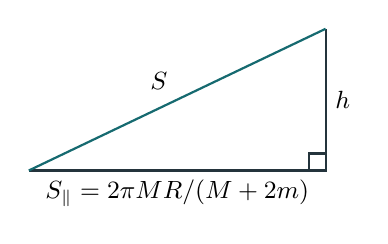
\begin{tikzpicture}[scale=1.8]
\draw[object] (0,0)--(2.0943951,0)--(2.0943951,1);
\draw[traj] (0,0)--(2.0943951,1);
\draw[object] (1.9743951,0)--(1.9743951,.12)--(2.0943951,.12);
\node[below] at (1.0471976,0) {$S_\parallel=2\pi MR/(M+2m)$};
\node[right] at (2.0943951,.5) {$h$};
\node[above left] at (1.0471976,.5) {$S$};
\end{tikzpicture}
\figcaption{解图力试1.3D\quad 地面螺旋展开后的水平弧长、下降量与总路程}
\end{minipage}\end{center}
地面水平长度包含两个因素：半径由$R$缩成$MR/(M+m)$，方位角由相对一周缩成$2\pi(M+m)/(M+2m)$。两者相乘才出现$M+2m$。当$M$很大时，筒轴半径趋零、反向自转趋零，球的路程趋向固定槽长$\sqrt{h^2+4\pi^2R^2}$；对任意有限正质量，地面水平弧长较小，重力只改变通过这条固定几何轨迹的快慢。


\Needspace{8\baselineskip}

\pdfbookmark[3]{关键洞察}{q3-h5}

\subsection*{关键洞察}

相对圆筒绕一周给的是$\varphi=2\pi$，地面角还含筒的反向自转。圆筒平移同时使球绕固定质心的半径缩短，两个变化共同形成路程中的$M+2m$。

\Needspace{8\baselineskip}

\pdfbookmark[3]{易错点}{q3-h6}

\subsection*{易错点}

\begin{itemize}
\item 球和筒轴都绕水平质心公转，两项公转角动量共同进入守恒式。
\item 筒轴公转与筒自身转动分开计角，按同一正向保留筒自转的负号。
\item 球的水平速率为$r_m\dot\theta$，完整速度还含竖直下降分量。
\item 槽的相对长度与球的地面长度使用不同半径和角度。
\item 水平、竖直微元比例为常数后，展开轨迹成为直线，投影总长度才按勾股合成。\end{itemize}

\Needspace{8\baselineskip}

\pdfbookmark[3]{课堂讲解建议}{q3-h7}

\subsection*{课堂讲解建议}

先在A图让学生用水平质心关系找固定点，分别画球公转、轴公转和筒壁标记点的速度。把三项角动量写在对应对象旁，再在B图读出每个角的符号与比例。用相等质量例子给出三分之二周与反向三分之一周，放到C图观察实际螺旋；最后逐段标同一个相对角微元，将地面水平弧长和下降量放入D图积分。

\Needspace{8\baselineskip}

\pdfbookmark[3]{变式训练}{q3-h8}

\subsection*{变式训练}

\begin{enumerate}
\item \textbf{相等质量的角度和路程。}若$M=m$，求球与筒轴的公转半径、终角及小球地面路程。

质心关系给$r_m=r_M=R/2$。球相对筒转一周时，角动量关系给
\[
 \Delta\theta=\frac{4\pi}{3},\qquad
 \Delta\psi=-\frac{2\pi}{3},\qquad
 S_\parallel=\frac{2\pi R}{3},\qquad
 S=\sqrt{h^2+\frac{4\pi^2R^2}{9}}.
\]
变图力试1.3V1画三个角随相对进程的变化，末端球和筒轴公转三分之二周，筒反向自转三分之一周，两者的相对角正好一周。球的水平半径为$R/2$，与地面总角共同给水平弧长。
\begin{center}\begin{minipage}{.98\linewidth}\centering
\begin{tikzpicture}[scale=.88,transform shape]
\draw[axis] (0,0.6666666666666666)--(7.3,0.6666666666666666) node[right] {$\varphi/(2\pi)$};
\draw[axis] (0,0)--(0,2.8);
\node[above left] at (0,2.8) {$\text{带符号角}/(2\pi)$};
\draw[thin] (0.000000,0.6666666666666666)--(0.000000,0.6066666666666667);\node[below,font=\scriptsize] at (0.000000,0.5866666666666667) {$ 0 $};
\draw[thin] (1.750000,0.6666666666666666)--(1.750000,0.6066666666666667);\node[below,font=\scriptsize] at (1.750000,0.5866666666666667) {$ 0.25 $};
\draw[thin] (3.500000,0.6666666666666666)--(3.500000,0.6066666666666667);\node[below,font=\scriptsize] at (3.500000,0.5866666666666667) {$ 0.5 $};
\draw[thin] (5.250000,0.6666666666666666)--(5.250000,0.6066666666666667);\node[below,font=\scriptsize] at (5.250000,0.5866666666666667) {$ 0.75 $};
\draw[thin] (7.000000,0.6666666666666666)--(7.000000,0.6066666666666667);\node[below,font=\scriptsize] at (7.000000,0.5866666666666667) {$ 1 $};
\draw[thin] (0,0.111111)--(-.06,0.111111);\node[left,font=\scriptsize] at (-.08,0.111111) {$ -1/3 $};
\draw[thin] (0,0.666667)--(-.06,0.666667);\node[left,font=\scriptsize] at (-.08,0.666667) {$ 0 $};
\draw[thin] (0,1.222222)--(-.06,1.222222);\node[left,font=\scriptsize] at (-.08,1.222222) {$ 1/3 $};
\draw[thin] (0,1.777778)--(-.06,1.777778);\node[left,font=\scriptsize] at (-.08,1.777778) {$ 2/3 $};
\draw[thin] (0,2.333333)--(-.06,2.333333);\node[left,font=\scriptsize] at (-.08,2.333333) {$ 1 $};
\draw[thick,color=accent] plot coordinates {(0.0000000,0.6666667) (0.0291667,0.6712963) (0.0583333,0.6759259) (0.0875000,0.6805556) (0.1166667,0.6851852) (0.1458333,0.6898148) (0.1750000,0.6944444) (0.2041667,0.6990741) (0.2333333,0.7037037) (0.2625000,0.7083333) (0.2916667,0.7129630) (0.3208333,0.7175926) (0.3500000,0.7222222) (0.3791667,0.7268519) (0.4083333,0.7314815) (0.4375000,0.7361111) (0.4666667,0.7407407) (0.4958333,0.7453704) (0.5250000,0.7500000) (0.5541667,0.7546296) (0.5833333,0.7592593) (0.6125000,0.7638889) (0.6416667,0.7685185) (0.6708333,0.7731481) (0.7000000,0.7777778) (0.7291667,0.7824074) (0.7583333,0.7870370) (0.7875000,0.7916667) (0.8166667,0.7962963) (0.8458333,0.8009259) (0.8750000,0.8055556) (0.9041667,0.8101852) (0.9333333,0.8148148) (0.9625000,0.8194444) (0.9916667,0.8240741) (1.0208333,0.8287037) (1.0500000,0.8333333) (1.0791667,0.8379630) (1.1083333,0.8425926) (1.1375000,0.8472222) (1.1666667,0.8518519) (1.1958333,0.8564815) (1.2250000,0.8611111) (1.2541667,0.8657407) (1.2833333,0.8703704) (1.3125000,0.8750000) (1.3416667,0.8796296) (1.3708333,0.8842593) (1.4000000,0.8888889) (1.4291667,0.8935185) (1.4583333,0.8981481) (1.4875000,0.9027778) (1.5166667,0.9074074) (1.5458333,0.9120370) (1.5750000,0.9166667) (1.6041667,0.9212963) (1.6333333,0.9259259) (1.6625000,0.9305556) (1.6916667,0.9351852) (1.7208333,0.9398148) (1.7500000,0.9444444) (1.7791667,0.9490741) (1.8083333,0.9537037) (1.8375000,0.9583333) (1.8666667,0.9629630) (1.8958333,0.9675926) (1.9250000,0.9722222) (1.9541667,0.9768519) (1.9833333,0.9814815) (2.0125000,0.9861111) (2.0416667,0.9907407) (2.0708333,0.9953704) (2.1000000,1.0000000) (2.1291667,1.0046296) (2.1583333,1.0092593) (2.1875000,1.0138889) (2.2166667,1.0185185) (2.2458333,1.0231481) (2.2750000,1.0277778) (2.3041667,1.0324074) (2.3333333,1.0370370) (2.3625000,1.0416667) (2.3916667,1.0462963) (2.4208333,1.0509259) (2.4500000,1.0555556) (2.4791667,1.0601852) (2.5083333,1.0648148) (2.5375000,1.0694444) (2.5666667,1.0740741) (2.5958333,1.0787037) (2.6250000,1.0833333) (2.6541667,1.0879630) (2.6833333,1.0925926) (2.7125000,1.0972222) (2.7416667,1.1018519) (2.7708333,1.1064815) (2.8000000,1.1111111) (2.8291667,1.1157407) (2.8583333,1.1203704) (2.8875000,1.1250000) (2.9166667,1.1296296) (2.9458333,1.1342593) (2.9750000,1.1388889) (3.0041667,1.1435185) (3.0333333,1.1481481) (3.0625000,1.1527778) (3.0916667,1.1574074) (3.1208333,1.1620370) (3.1500000,1.1666667) (3.1791667,1.1712963) (3.2083333,1.1759259) (3.2375000,1.1805556) (3.2666667,1.1851852) (3.2958333,1.1898148) (3.3250000,1.1944444) (3.3541667,1.1990741) (3.3833333,1.2037037) (3.4125000,1.2083333) (3.4416667,1.2129630) (3.4708333,1.2175926) (3.5000000,1.2222222) (3.5291667,1.2268519) (3.5583333,1.2314815) (3.5875000,1.2361111) (3.6166667,1.2407407) (3.6458333,1.2453704) (3.6750000,1.2500000) (3.7041667,1.2546296) (3.7333333,1.2592593) (3.7625000,1.2638889) (3.7916667,1.2685185) (3.8208333,1.2731481) (3.8500000,1.2777778) (3.8791667,1.2824074) (3.9083333,1.2870370) (3.9375000,1.2916667) (3.9666667,1.2962963) (3.9958333,1.3009259) (4.0250000,1.3055556) (4.0541667,1.3101852) (4.0833333,1.3148148) (4.1125000,1.3194444) (4.1416667,1.3240741) (4.1708333,1.3287037) (4.2000000,1.3333333) (4.2291667,1.3379630) (4.2583333,1.3425926) (4.2875000,1.3472222) (4.3166667,1.3518519) (4.3458333,1.3564815) (4.3750000,1.3611111) (4.4041667,1.3657407) (4.4333333,1.3703704) (4.4625000,1.3750000) (4.4916667,1.3796296) (4.5208333,1.3842593) (4.5500000,1.3888889) (4.5791667,1.3935185) (4.6083333,1.3981481) (4.6375000,1.4027778) (4.6666667,1.4074074) (4.6958333,1.4120370) (4.7250000,1.4166667) (4.7541667,1.4212963) (4.7833333,1.4259259) (4.8125000,1.4305556) (4.8416667,1.4351852) (4.8708333,1.4398148) (4.9000000,1.4444444) (4.9291667,1.4490741) (4.9583333,1.4537037) (4.9875000,1.4583333) (5.0166667,1.4629630) (5.0458333,1.4675926) (5.0750000,1.4722222) (5.1041667,1.4768519) (5.1333333,1.4814815) (5.1625000,1.4861111) (5.1916667,1.4907407) (5.2208333,1.4953704) (5.2500000,1.5000000) (5.2791667,1.5046296) (5.3083333,1.5092593) (5.3375000,1.5138889) (5.3666667,1.5185185) (5.3958333,1.5231481) (5.4250000,1.5277778) (5.4541667,1.5324074) (5.4833333,1.5370370) (5.5125000,1.5416667) (5.5416667,1.5462963) (5.5708333,1.5509259) (5.6000000,1.5555556) (5.6291667,1.5601852) (5.6583333,1.5648148) (5.6875000,1.5694444) (5.7166667,1.5740741) (5.7458333,1.5787037) (5.7750000,1.5833333) (5.8041667,1.5879630) (5.8333333,1.5925926) (5.8625000,1.5972222) (5.8916667,1.6018519) (5.9208333,1.6064815) (5.9500000,1.6111111) (5.9791667,1.6157407) (6.0083333,1.6203704) (6.0375000,1.6250000) (6.0666667,1.6296296) (6.0958333,1.6342593) (6.1250000,1.6388889) (6.1541667,1.6435185) (6.1833333,1.6481481) (6.2125000,1.6527778) (6.2416667,1.6574074) (6.2708333,1.6620370) (6.3000000,1.6666667) (6.3291667,1.6712963) (6.3583333,1.6759259) (6.3875000,1.6805556) (6.4166667,1.6851852) (6.4458333,1.6898148) (6.4750000,1.6944444) (6.5041667,1.6990741) (6.5333333,1.7037037) (6.5625000,1.7083333) (6.5916667,1.7129630) (6.6208333,1.7175926) (6.6500000,1.7222222) (6.6791667,1.7268519) (6.7083333,1.7314815) (6.7375000,1.7361111) (6.7666667,1.7407407) (6.7958333,1.7453704) (6.8250000,1.7500000) (6.8541667,1.7546296) (6.8833333,1.7592593) (6.9125000,1.7638889) (6.9416667,1.7685185) (6.9708333,1.7731481) (7.0000000,1.7777778)};
\draw[thick,color=accent] (7.65,2.55)--(8.15,2.55);\node[right,font=\scriptsize] at (8.2,2.55) {$\theta/(2\pi)$};
\draw[thick,dashed,color=warm] plot coordinates {(0.0000000,0.6666667) (0.0291667,0.6643519) (0.0583333,0.6620370) (0.0875000,0.6597222) (0.1166667,0.6574074) (0.1458333,0.6550926) (0.1750000,0.6527778) (0.2041667,0.6504630) (0.2333333,0.6481481) (0.2625000,0.6458333) (0.2916667,0.6435185) (0.3208333,0.6412037) (0.3500000,0.6388889) (0.3791667,0.6365741) (0.4083333,0.6342593) (0.4375000,0.6319444) (0.4666667,0.6296296) (0.4958333,0.6273148) (0.5250000,0.6250000) (0.5541667,0.6226852) (0.5833333,0.6203704) (0.6125000,0.6180556) (0.6416667,0.6157407) (0.6708333,0.6134259) (0.7000000,0.6111111) (0.7291667,0.6087963) (0.7583333,0.6064815) (0.7875000,0.6041667) (0.8166667,0.6018519) (0.8458333,0.5995370) (0.8750000,0.5972222) (0.9041667,0.5949074) (0.9333333,0.5925926) (0.9625000,0.5902778) (0.9916667,0.5879630) (1.0208333,0.5856481) (1.0500000,0.5833333) (1.0791667,0.5810185) (1.1083333,0.5787037) (1.1375000,0.5763889) (1.1666667,0.5740741) (1.1958333,0.5717593) (1.2250000,0.5694444) (1.2541667,0.5671296) (1.2833333,0.5648148) (1.3125000,0.5625000) (1.3416667,0.5601852) (1.3708333,0.5578704) (1.4000000,0.5555556) (1.4291667,0.5532407) (1.4583333,0.5509259) (1.4875000,0.5486111) (1.5166667,0.5462963) (1.5458333,0.5439815) (1.5750000,0.5416667) (1.6041667,0.5393519) (1.6333333,0.5370370) (1.6625000,0.5347222) (1.6916667,0.5324074) (1.7208333,0.5300926) (1.7500000,0.5277778) (1.7791667,0.5254630) (1.8083333,0.5231481) (1.8375000,0.5208333) (1.8666667,0.5185185) (1.8958333,0.5162037) (1.9250000,0.5138889) (1.9541667,0.5115741) (1.9833333,0.5092593) (2.0125000,0.5069444) (2.0416667,0.5046296) (2.0708333,0.5023148) (2.1000000,0.5000000) (2.1291667,0.4976852) (2.1583333,0.4953704) (2.1875000,0.4930556) (2.2166667,0.4907407) (2.2458333,0.4884259) (2.2750000,0.4861111) (2.3041667,0.4837963) (2.3333333,0.4814815) (2.3625000,0.4791667) (2.3916667,0.4768519) (2.4208333,0.4745370) (2.4500000,0.4722222) (2.4791667,0.4699074) (2.5083333,0.4675926) (2.5375000,0.4652778) (2.5666667,0.4629630) (2.5958333,0.4606481) (2.6250000,0.4583333) (2.6541667,0.4560185) (2.6833333,0.4537037) (2.7125000,0.4513889) (2.7416667,0.4490741) (2.7708333,0.4467593) (2.8000000,0.4444444) (2.8291667,0.4421296) (2.8583333,0.4398148) (2.8875000,0.4375000) (2.9166667,0.4351852) (2.9458333,0.4328704) (2.9750000,0.4305556) (3.0041667,0.4282407) (3.0333333,0.4259259) (3.0625000,0.4236111) (3.0916667,0.4212963) (3.1208333,0.4189815) (3.1500000,0.4166667) (3.1791667,0.4143519) (3.2083333,0.4120370) (3.2375000,0.4097222) (3.2666667,0.4074074) (3.2958333,0.4050926) (3.3250000,0.4027778) (3.3541667,0.4004630) (3.3833333,0.3981481) (3.4125000,0.3958333) (3.4416667,0.3935185) (3.4708333,0.3912037) (3.5000000,0.3888889) (3.5291667,0.3865741) (3.5583333,0.3842593) (3.5875000,0.3819444) (3.6166667,0.3796296) (3.6458333,0.3773148) (3.6750000,0.3750000) (3.7041667,0.3726852) (3.7333333,0.3703704) (3.7625000,0.3680556) (3.7916667,0.3657407) (3.8208333,0.3634259) (3.8500000,0.3611111) (3.8791667,0.3587963) (3.9083333,0.3564815) (3.9375000,0.3541667) (3.9666667,0.3518519) (3.9958333,0.3495370) (4.0250000,0.3472222) (4.0541667,0.3449074) (4.0833333,0.3425926) (4.1125000,0.3402778) (4.1416667,0.3379630) (4.1708333,0.3356481) (4.2000000,0.3333333) (4.2291667,0.3310185) (4.2583333,0.3287037) (4.2875000,0.3263889) (4.3166667,0.3240741) (4.3458333,0.3217593) (4.3750000,0.3194444) (4.4041667,0.3171296) (4.4333333,0.3148148) (4.4625000,0.3125000) (4.4916667,0.3101852) (4.5208333,0.3078704) (4.5500000,0.3055556) (4.5791667,0.3032407) (4.6083333,0.3009259) (4.6375000,0.2986111) (4.6666667,0.2962963) (4.6958333,0.2939815) (4.7250000,0.2916667) (4.7541667,0.2893519) (4.7833333,0.2870370) (4.8125000,0.2847222) (4.8416667,0.2824074) (4.8708333,0.2800926) (4.9000000,0.2777778) (4.9291667,0.2754630) (4.9583333,0.2731481) (4.9875000,0.2708333) (5.0166667,0.2685185) (5.0458333,0.2662037) (5.0750000,0.2638889) (5.1041667,0.2615741) (5.1333333,0.2592593) (5.1625000,0.2569444) (5.1916667,0.2546296) (5.2208333,0.2523148) (5.2500000,0.2500000) (5.2791667,0.2476852) (5.3083333,0.2453704) (5.3375000,0.2430556) (5.3666667,0.2407407) (5.3958333,0.2384259) (5.4250000,0.2361111) (5.4541667,0.2337963) (5.4833333,0.2314815) (5.5125000,0.2291667) (5.5416667,0.2268519) (5.5708333,0.2245370) (5.6000000,0.2222222) (5.6291667,0.2199074) (5.6583333,0.2175926) (5.6875000,0.2152778) (5.7166667,0.2129630) (5.7458333,0.2106481) (5.7750000,0.2083333) (5.8041667,0.2060185) (5.8333333,0.2037037) (5.8625000,0.2013889) (5.8916667,0.1990741) (5.9208333,0.1967593) (5.9500000,0.1944444) (5.9791667,0.1921296) (6.0083333,0.1898148) (6.0375000,0.1875000) (6.0666667,0.1851852) (6.0958333,0.1828704) (6.1250000,0.1805556) (6.1541667,0.1782407) (6.1833333,0.1759259) (6.2125000,0.1736111) (6.2416667,0.1712963) (6.2708333,0.1689815) (6.3000000,0.1666667) (6.3291667,0.1643519) (6.3583333,0.1620370) (6.3875000,0.1597222) (6.4166667,0.1574074) (6.4458333,0.1550926) (6.4750000,0.1527778) (6.5041667,0.1504630) (6.5333333,0.1481481) (6.5625000,0.1458333) (6.5916667,0.1435185) (6.6208333,0.1412037) (6.6500000,0.1388889) (6.6791667,0.1365741) (6.7083333,0.1342593) (6.7375000,0.1319444) (6.7666667,0.1296296) (6.7958333,0.1273148) (6.8250000,0.1250000) (6.8541667,0.1226852) (6.8833333,0.1203704) (6.9125000,0.1180556) (6.9416667,0.1157407) (6.9708333,0.1134259) (7.0000000,0.1111111)};
\draw[thick,dashed,color=warm] (7.65,2.0999999999999996)--(8.15,2.0999999999999996);\node[right,font=\scriptsize] at (8.2,2.0999999999999996) {$\psi/(2\pi)$};
\draw[densely dotted,thick,color=muted] plot coordinates {(0.0000000,0.6666667) (0.0291667,0.6736111) (0.0583333,0.6805556) (0.0875000,0.6875000) (0.1166667,0.6944444) (0.1458333,0.7013889) (0.1750000,0.7083333) (0.2041667,0.7152778) (0.2333333,0.7222222) (0.2625000,0.7291667) (0.2916667,0.7361111) (0.3208333,0.7430556) (0.3500000,0.7500000) (0.3791667,0.7569444) (0.4083333,0.7638889) (0.4375000,0.7708333) (0.4666667,0.7777778) (0.4958333,0.7847222) (0.5250000,0.7916667) (0.5541667,0.7986111) (0.5833333,0.8055556) (0.6125000,0.8125000) (0.6416667,0.8194444) (0.6708333,0.8263889) (0.7000000,0.8333333) (0.7291667,0.8402778) (0.7583333,0.8472222) (0.7875000,0.8541667) (0.8166667,0.8611111) (0.8458333,0.8680556) (0.8750000,0.8750000) (0.9041667,0.8819444) (0.9333333,0.8888889) (0.9625000,0.8958333) (0.9916667,0.9027778) (1.0208333,0.9097222) (1.0500000,0.9166667) (1.0791667,0.9236111) (1.1083333,0.9305556) (1.1375000,0.9375000) (1.1666667,0.9444444) (1.1958333,0.9513889) (1.2250000,0.9583333) (1.2541667,0.9652778) (1.2833333,0.9722222) (1.3125000,0.9791667) (1.3416667,0.9861111) (1.3708333,0.9930556) (1.4000000,1.0000000) (1.4291667,1.0069444) (1.4583333,1.0138889) (1.4875000,1.0208333) (1.5166667,1.0277778) (1.5458333,1.0347222) (1.5750000,1.0416667) (1.6041667,1.0486111) (1.6333333,1.0555556) (1.6625000,1.0625000) (1.6916667,1.0694444) (1.7208333,1.0763889) (1.7500000,1.0833333) (1.7791667,1.0902778) (1.8083333,1.0972222) (1.8375000,1.1041667) (1.8666667,1.1111111) (1.8958333,1.1180556) (1.9250000,1.1250000) (1.9541667,1.1319444) (1.9833333,1.1388889) (2.0125000,1.1458333) (2.0416667,1.1527778) (2.0708333,1.1597222) (2.1000000,1.1666667) (2.1291667,1.1736111) (2.1583333,1.1805556) (2.1875000,1.1875000) (2.2166667,1.1944444) (2.2458333,1.2013889) (2.2750000,1.2083333) (2.3041667,1.2152778) (2.3333333,1.2222222) (2.3625000,1.2291667) (2.3916667,1.2361111) (2.4208333,1.2430556) (2.4500000,1.2500000) (2.4791667,1.2569444) (2.5083333,1.2638889) (2.5375000,1.2708333) (2.5666667,1.2777778) (2.5958333,1.2847222) (2.6250000,1.2916667) (2.6541667,1.2986111) (2.6833333,1.3055556) (2.7125000,1.3125000) (2.7416667,1.3194444) (2.7708333,1.3263889) (2.8000000,1.3333333) (2.8291667,1.3402778) (2.8583333,1.3472222) (2.8875000,1.3541667) (2.9166667,1.3611111) (2.9458333,1.3680556) (2.9750000,1.3750000) (3.0041667,1.3819444) (3.0333333,1.3888889) (3.0625000,1.3958333) (3.0916667,1.4027778) (3.1208333,1.4097222) (3.1500000,1.4166667) (3.1791667,1.4236111) (3.2083333,1.4305556) (3.2375000,1.4375000) (3.2666667,1.4444444) (3.2958333,1.4513889) (3.3250000,1.4583333) (3.3541667,1.4652778) (3.3833333,1.4722222) (3.4125000,1.4791667) (3.4416667,1.4861111) (3.4708333,1.4930556) (3.5000000,1.5000000) (3.5291667,1.5069444) (3.5583333,1.5138889) (3.5875000,1.5208333) (3.6166667,1.5277778) (3.6458333,1.5347222) (3.6750000,1.5416667) (3.7041667,1.5486111) (3.7333333,1.5555556) (3.7625000,1.5625000) (3.7916667,1.5694444) (3.8208333,1.5763889) (3.8500000,1.5833333) (3.8791667,1.5902778) (3.9083333,1.5972222) (3.9375000,1.6041667) (3.9666667,1.6111111) (3.9958333,1.6180556) (4.0250000,1.6250000) (4.0541667,1.6319444) (4.0833333,1.6388889) (4.1125000,1.6458333) (4.1416667,1.6527778) (4.1708333,1.6597222) (4.2000000,1.6666667) (4.2291667,1.6736111) (4.2583333,1.6805556) (4.2875000,1.6875000) (4.3166667,1.6944444) (4.3458333,1.7013889) (4.3750000,1.7083333) (4.4041667,1.7152778) (4.4333333,1.7222222) (4.4625000,1.7291667) (4.4916667,1.7361111) (4.5208333,1.7430556) (4.5500000,1.7500000) (4.5791667,1.7569444) (4.6083333,1.7638889) (4.6375000,1.7708333) (4.6666667,1.7777778) (4.6958333,1.7847222) (4.7250000,1.7916667) (4.7541667,1.7986111) (4.7833333,1.8055556) (4.8125000,1.8125000) (4.8416667,1.8194444) (4.8708333,1.8263889) (4.9000000,1.8333333) (4.9291667,1.8402778) (4.9583333,1.8472222) (4.9875000,1.8541667) (5.0166667,1.8611111) (5.0458333,1.8680556) (5.0750000,1.8750000) (5.1041667,1.8819444) (5.1333333,1.8888889) (5.1625000,1.8958333) (5.1916667,1.9027778) (5.2208333,1.9097222) (5.2500000,1.9166667) (5.2791667,1.9236111) (5.3083333,1.9305556) (5.3375000,1.9375000) (5.3666667,1.9444444) (5.3958333,1.9513889) (5.4250000,1.9583333) (5.4541667,1.9652778) (5.4833333,1.9722222) (5.5125000,1.9791667) (5.5416667,1.9861111) (5.5708333,1.9930556) (5.6000000,2.0000000) (5.6291667,2.0069444) (5.6583333,2.0138889) (5.6875000,2.0208333) (5.7166667,2.0277778) (5.7458333,2.0347222) (5.7750000,2.0416667) (5.8041667,2.0486111) (5.8333333,2.0555556) (5.8625000,2.0625000) (5.8916667,2.0694444) (5.9208333,2.0763889) (5.9500000,2.0833333) (5.9791667,2.0902778) (6.0083333,2.0972222) (6.0375000,2.1041667) (6.0666667,2.1111111) (6.0958333,2.1180556) (6.1250000,2.1250000) (6.1541667,2.1319444) (6.1833333,2.1388889) (6.2125000,2.1458333) (6.2416667,2.1527778) (6.2708333,2.1597222) (6.3000000,2.1666667) (6.3291667,2.1736111) (6.3583333,2.1805556) (6.3875000,2.1875000) (6.4166667,2.1944444) (6.4458333,2.2013889) (6.4750000,2.2083333) (6.5041667,2.2152778) (6.5333333,2.2222222) (6.5625000,2.2291667) (6.5916667,2.2361111) (6.6208333,2.2430556) (6.6500000,2.2500000) (6.6791667,2.2569444) (6.7083333,2.2638889) (6.7375000,2.2708333) (6.7666667,2.2777778) (6.7958333,2.2847222) (6.8250000,2.2916667) (6.8541667,2.2986111) (6.8833333,2.3055556) (6.9125000,2.3125000) (6.9416667,2.3194444) (6.9708333,2.3263889) (7.0000000,2.3333333)};
\draw[densely dotted,thick,color=muted] (7.65,1.65)--(8.15,1.65);\node[right,font=\scriptsize] at (8.2,1.65) {$\varphi/(2\pi)$};
\end{tikzpicture}
\figcaption{变图力试1.3V1\quad 相等质量时相对一周与地面三分之二周}
\end{minipage}\end{center}
\item \textbf{任意轴向转动惯量。}保持筒质量、半径和槽形，令筒轴惯量为$I>0$，求地面路程。

水平质心关系保持，令$\mu=Mm/(M+m)$。角动量$\mu R^2\dot\theta+I\dot\psi=0$与$\dot\theta=\dot\varphi+\dot\psi$给
\[
 \lambda=\frac{I}{I+\mu R^2},\qquad
 \theta=\lambda\varphi,\quad \psi=-(1-\lambda)\varphi,\qquad
 S=\sqrt{h^2+(2\pi r_m\lambda)^2}.
\]
变图力试1.3V2取$M=m,h=R$，横轴为$I/(MR^2)$。惯量增加使反向自转比例减小，地面水平总角与路程增大；$I=MR^2$给$\lambda=2/3$，回到主解。
\begin{center}\begin{minipage}{.98\linewidth}\centering
\begin{tikzpicture}[scale=.88,transform shape]
\draw[axis] (0,0.0)--(7.3,0.0) node[right] {$I/(MR^2)$};
\draw[axis] (0,0)--(0,2.8);
\node[above left] at (0,2.8) {$S/R$};
\draw[thin] (0.000000,0.0)--(0.000000,-0.06);\node[below,font=\scriptsize] at (0.000000,-0.08) {$ 0.1 $};
\draw[thin] (0.965517,0.0)--(0.965517,-0.06);\node[below,font=\scriptsize] at (0.965517,-0.08) {$ 0.5 $};
\draw[thin] (2.172414,0.0)--(2.172414,-0.06);\node[below,font=\scriptsize] at (2.172414,-0.08) {$ 1 $};
\draw[thin] (4.586207,0.0)--(4.586207,-0.06);\node[below,font=\scriptsize] at (4.586207,-0.08) {$ 2 $};
\draw[thin] (7.000000,0.0)--(7.000000,-0.06);\node[below,font=\scriptsize] at (7.000000,-0.08) {$ 3 $};
\draw[thin] (0,0.000000)--(-.06,0.000000);\node[left,font=\scriptsize] at (-.08,0.000000) {$ 0 $};
\draw[thin] (0,0.833333)--(-.06,0.833333);\node[left,font=\scriptsize] at (-.08,0.833333) {$ 1 $};
\draw[thin] (0,1.666667)--(-.06,1.666667);\node[left,font=\scriptsize] at (-.08,1.666667) {$ 2 $};
\draw[thin] (0,2.500000)--(-.06,2.500000);\node[left,font=\scriptsize] at (-.08,2.500000) {$ 3 $};
\draw[thick,color=accent] plot coordinates {(0.0000000,0.9406542) (0.0291667,0.9613896) (0.0583333,0.9826900) (0.0875000,1.0043664) (0.1166667,1.0262631) (0.1458333,1.0482529) (0.1750000,1.0702322) (0.2041667,1.0921172) (0.2333333,1.1138405) (0.2625000,1.1353484) (0.2916667,1.1565983) (0.3208333,1.1775571) (0.3500000,1.1981991) (0.3791667,1.2185052) (0.4083333,1.2384613) (0.4375000,1.2580576) (0.4666667,1.2772878) (0.4958333,1.2961485) (0.5250000,1.3146386) (0.5541667,1.3327589) (0.5833333,1.3505117) (0.6125000,1.3679008) (0.6416667,1.3849305) (0.6708333,1.4016063) (0.7000000,1.4179341) (0.7291667,1.4339204) (0.7583333,1.4495719) (0.7875000,1.4648958) (0.8166667,1.4798991) (0.8458333,1.4945892) (0.8750000,1.5089735) (0.9041667,1.5230593) (0.9333333,1.5368540) (0.9625000,1.5503648) (0.9916667,1.5635989) (1.0208333,1.5765634) (1.0500000,1.5892652) (1.0791667,1.6017112) (1.1083333,1.6139079) (1.1375000,1.6258620) (1.1666667,1.6375798) (1.1958333,1.6490675) (1.2250000,1.6603311) (1.2541667,1.6713766) (1.2833333,1.6822096) (1.3125000,1.6928358) (1.3416667,1.7032605) (1.3708333,1.7134889) (1.4000000,1.7235263) (1.4291667,1.7333776) (1.4583333,1.7430474) (1.4875000,1.7525406) (1.5166667,1.7618617) (1.5458333,1.7710149) (1.5750000,1.7800046) (1.6041667,1.7888350) (1.6333333,1.7975099) (1.6625000,1.8060333) (1.6916667,1.8144090) (1.7208333,1.8226406) (1.7500000,1.8307316) (1.7791667,1.8386854) (1.8083333,1.8465055) (1.8375000,1.8541950) (1.8666667,1.8617570) (1.8958333,1.8691947) (1.9250000,1.8765108) (1.9541667,1.8837084) (1.9833333,1.8907902) (2.0125000,1.8977588) (2.0416667,1.9046169) (2.0708333,1.9113671) (2.1000000,1.9180117) (2.1291667,1.9245533) (2.1583333,1.9309940) (2.1875000,1.9373362) (2.2166667,1.9435820) (2.2458333,1.9497337) (2.2750000,1.9557932) (2.3041667,1.9617626) (2.3333333,1.9676438) (2.3625000,1.9734387) (2.3916667,1.9791492) (2.4208333,1.9847771) (2.4500000,1.9903242) (2.4791667,1.9957920) (2.5083333,2.0011823) (2.5375000,2.0064968) (2.5666667,2.0117369) (2.5958333,2.0169041) (2.6250000,2.0220001) (2.6541667,2.0270261) (2.6833333,2.0319837) (2.7125000,2.0368741) (2.7416667,2.0416988) (2.7708333,2.0464590) (2.8000000,2.0511560) (2.8291667,2.0557911) (2.8583333,2.0603653) (2.8875000,2.0648800) (2.9166667,2.0693362) (2.9458333,2.0737351) (2.9750000,2.0780778) (3.0041667,2.0823652) (3.0333333,2.0865985) (3.0625000,2.0907786) (3.0916667,2.0949066) (3.1208333,2.0989834) (3.1500000,2.1030099) (3.1791667,2.1069871) (3.2083333,2.1109158) (3.2375000,2.1147970) (3.2666667,2.1186314) (3.2958333,2.1224199) (3.3250000,2.1261633) (3.3541667,2.1298624) (3.3833333,2.1335180) (3.4125000,2.1371308) (3.4416667,2.1407016) (3.4708333,2.1442312) (3.5000000,2.1477201) (3.5291667,2.1511691) (3.5583333,2.1545789) (3.5875000,2.1579501) (3.6166667,2.1612834) (3.6458333,2.1645795) (3.6750000,2.1678388) (3.7041667,2.1710621) (3.7333333,2.1742499) (3.7625000,2.1774028) (3.7916667,2.1805214) (3.8208333,2.1836062) (3.8500000,2.1866578) (3.8791667,2.1896767) (3.9083333,2.1926634) (3.9375000,2.1956184) (3.9666667,2.1985423) (3.9958333,2.2014354) (4.0250000,2.2042984) (4.0541667,2.2071316) (4.0833333,2.2099355) (4.1125000,2.2127106) (4.1416667,2.2154573) (4.1708333,2.2181761) (4.2000000,2.2208673) (4.2291667,2.2235314) (4.2583333,2.2261687) (4.2875000,2.2287798) (4.3166667,2.2313649) (4.3458333,2.2339245) (4.3750000,2.2364588) (4.4041667,2.2389684) (4.4333333,2.2414536) (4.4625000,2.2439146) (4.4916667,2.2463519) (4.5208333,2.2487658) (4.5500000,2.2511567) (4.5791667,2.2535248) (4.6083333,2.2558704) (4.6375000,2.2581940) (4.6666667,2.2604958) (4.6958333,2.2627761) (4.7250000,2.2650352) (4.7541667,2.2672734) (4.7833333,2.2694910) (4.8125000,2.2716882) (4.8416667,2.2738654) (4.8708333,2.2760229) (4.9000000,2.2781608) (4.9291667,2.2802794) (4.9583333,2.2823791) (4.9875000,2.2844600) (5.0166667,2.2865225) (5.0458333,2.2885667) (5.0750000,2.2905929) (5.1041667,2.2926013) (5.1333333,2.2945922) (5.1625000,2.2965658) (5.1916667,2.2985223) (5.2208333,2.3004619) (5.2500000,2.3023849) (5.2791667,2.3042915) (5.3083333,2.3061818) (5.3375000,2.3080561) (5.3666667,2.3099146) (5.3958333,2.3117575) (5.4250000,2.3135849) (5.4541667,2.3153971) (5.4833333,2.3171943) (5.5125000,2.3189766) (5.5416667,2.3207442) (5.5708333,2.3224974) (5.6000000,2.3242362) (5.6291667,2.3259609) (5.6583333,2.3276716) (5.6875000,2.3293685) (5.7166667,2.3310518) (5.7458333,2.3327216) (5.7750000,2.3343781) (5.8041667,2.3360215) (5.8333333,2.3376518) (5.8625000,2.3392693) (5.8916667,2.3408741) (5.9208333,2.3424664) (5.9500000,2.3440462) (5.9791667,2.3456138) (6.0083333,2.3471693) (6.0375000,2.3487128) (6.0666667,2.3502445) (6.0958333,2.3517645) (6.1250000,2.3532729) (6.1541667,2.3547699) (6.1833333,2.3562555) (6.2125000,2.3577300) (6.2416667,2.3591934) (6.2708333,2.3606459) (6.3000000,2.3620876) (6.3291667,2.3635186) (6.3583333,2.3649391) (6.3875000,2.3663490) (6.4166667,2.3677487) (6.4458333,2.3691381) (6.4750000,2.3705174) (6.5041667,2.3718866) (6.5333333,2.3732460) (6.5625000,2.3745956) (6.5916667,2.3759355) (6.6208333,2.3772659) (6.6500000,2.3785867) (6.6791667,2.3798982) (6.7083333,2.3812004) (6.7375000,2.3824934) (6.7666667,2.3837773) (6.7958333,2.3850523) (6.8250000,2.3863183) (6.8541667,2.3875755) (6.8833333,2.3888241) (6.9125000,2.3900640) (6.9416667,2.3912953) (6.9708333,2.3925183) (7.0000000,2.3937328)};
\end{tikzpicture}
\figcaption{变图力试1.3V2\quad 相等质量且h等于R时路程随自转惯量变化}
\end{minipage}\end{center}
\item \textbf{固定筒轴而允许自转。}圆筒轴线由无摩擦轴承固定，仍能绕竖直轴自转，求小球地面路程。

轴承承担水平反作用力，球的地面水平半径为$R$。关于固定轴的外力矩为零，故$mR^2(\dot\varphi+\dot\psi)+I\dot\psi=0$。对薄壁筒$I=MR^2$，
\[
 \theta=\frac{M}{M+m}\varphi,\qquad
 S_{\rm fixed}=\sqrt{h^2+
 \left(\frac{2\pi MR}{M+m}\right)^2}.
\]
变图力试1.3V3在$h=R$时比较可平移与固定轴两种路程。相等质量时固定轴水平长度为$\pi R$，可平移时为$2\pi R/3$；质心位置关系和公转角动量的改变分别进入两式。
\begin{center}\begin{minipage}{.98\linewidth}\centering
\begin{tikzpicture}[scale=.88,transform shape]
\draw[axis] (0,0.0)--(7.3,0.0) node[right] {$M/m$};
\draw[axis] (0,0)--(0,2.8);
\node[above left] at (0,2.8) {$S/R$};
\draw[thin] (0.000000,0.0)--(0.000000,-0.06);\node[below,font=\scriptsize] at (0.000000,-0.08) {$ 0.1 $};
\draw[thin] (1.285714,0.0)--(1.285714,-0.06);\node[below,font=\scriptsize] at (1.285714,-0.08) {$ 1 $};
\draw[thin] (2.714286,0.0)--(2.714286,-0.06);\node[below,font=\scriptsize] at (2.714286,-0.08) {$ 2 $};
\draw[thin] (4.142857,0.0)--(4.142857,-0.06);\node[below,font=\scriptsize] at (4.142857,-0.08) {$ 3 $};
\draw[thin] (7.000000,0.0)--(7.000000,-0.06);\node[below,font=\scriptsize] at (7.000000,-0.08) {$ 5 $};
\draw[thin] (0,0.000000)--(-.06,0.000000);\node[left,font=\scriptsize] at (-.08,0.000000) {$ 0 $};
\draw[thin] (0,0.454545)--(-.06,0.454545);\node[left,font=\scriptsize] at (-.08,0.454545) {$ 1 $};
\draw[thin] (0,0.909091)--(-.06,0.909091);\node[left,font=\scriptsize] at (-.08,0.909091) {$ 2 $};
\draw[thin] (0,1.363636)--(-.06,1.363636);\node[left,font=\scriptsize] at (-.08,1.363636) {$ 3 $};
\draw[thin] (0,1.818182)--(-.06,1.818182);\node[left,font=\scriptsize] at (-.08,1.818182) {$ 4 $};
\draw[thin] (0,2.272727)--(-.06,2.272727);\node[left,font=\scriptsize] at (-.08,2.272727) {$ 5 $};
\draw[thick,color=accent] plot coordinates {(0.0000000,0.4744549) (0.0291667,0.4826147) (0.0583333,0.4918438) (0.0875000,0.5020125) (0.1166667,0.5129998) (0.1458333,0.5246940) (0.1750000,0.5369936) (0.2041667,0.5498068) (0.2333333,0.5630513) (0.2625000,0.5766541) (0.2916667,0.5905501) (0.3208333,0.6046823) (0.3500000,0.6190002) (0.3791667,0.6334597) (0.4083333,0.6480221) (0.4375000,0.6626536) (0.4666667,0.6773248) (0.4958333,0.6920100) (0.5250000,0.7066869) (0.5541667,0.7213360) (0.5833333,0.7359407) (0.6125000,0.7504863) (0.6416667,0.7649603) (0.6708333,0.7793518) (0.7000000,0.7936516) (0.7291667,0.8078518) (0.7583333,0.8219455) (0.7875000,0.8359270) (0.8166667,0.8497916) (0.8458333,0.8635350) (0.8750000,0.8771541) (0.9041667,0.8906460) (0.9333333,0.9040087) (0.9625000,0.9172404) (0.9916667,0.9303398) (1.0208333,0.9433060) (1.0500000,0.9561385) (1.0791667,0.9688368) (1.1083333,0.9814011) (1.1375000,0.9938313) (1.1666667,1.0061280) (1.1958333,1.0182916) (1.2250000,1.0303227) (1.2541667,1.0422223) (1.2833333,1.0539911) (1.3125000,1.0656303) (1.3416667,1.0771409) (1.3708333,1.0885240) (1.4000000,1.0997809) (1.4291667,1.1109129) (1.4583333,1.1219213) (1.4875000,1.1328074) (1.5166667,1.1435727) (1.5458333,1.1542185) (1.5750000,1.1647463) (1.6041667,1.1751575) (1.6333333,1.1854536) (1.6625000,1.1956360) (1.6916667,1.2057062) (1.7208333,1.2156656) (1.7500000,1.2255159) (1.7791667,1.2352582) (1.8083333,1.2448943) (1.8375000,1.2544254) (1.8666667,1.2638530) (1.8958333,1.2731786) (1.9250000,1.2824036) (1.9541667,1.2915293) (1.9833333,1.3005571) (2.0125000,1.3094885) (2.0416667,1.3183247) (2.0708333,1.3270671) (2.1000000,1.3357171) (2.1291667,1.3442759) (2.1583333,1.3527449) (2.1875000,1.3611253) (2.2166667,1.3694183) (2.2458333,1.3776252) (2.2750000,1.3857473) (2.3041667,1.3937856) (2.3333333,1.4017415) (2.3625000,1.4096161) (2.3916667,1.4174105) (2.4208333,1.4251259) (2.4500000,1.4327633) (2.4791667,1.4403239) (2.5083333,1.4478088) (2.5375000,1.4552190) (2.5666667,1.4625556) (2.5958333,1.4698195) (2.6250000,1.4770119) (2.6541667,1.4841337) (2.6833333,1.4911858) (2.7125000,1.4981693) (2.7416667,1.5050851) (2.7708333,1.5119342) (2.8000000,1.5187174) (2.8291667,1.5254357) (2.8583333,1.5320899) (2.8875000,1.5386809) (2.9166667,1.5452096) (2.9458333,1.5516768) (2.9750000,1.5580834) (3.0041667,1.5644302) (3.0333333,1.5707179) (3.0625000,1.5769474) (3.0916667,1.5831195) (3.1208333,1.5892348) (3.1500000,1.5952943) (3.1791667,1.6012985) (3.2083333,1.6072482) (3.2375000,1.6131442) (3.2666667,1.6189872) (3.2958333,1.6247778) (3.3250000,1.6305167) (3.3541667,1.6362046) (3.3833333,1.6418422) (3.4125000,1.6474301) (3.4416667,1.6529689) (3.4708333,1.6584592) (3.5000000,1.6639018) (3.5291667,1.6692972) (3.5583333,1.6746459) (3.5875000,1.6799486) (3.6166667,1.6852059) (3.6458333,1.6904183) (3.6750000,1.6955864) (3.7041667,1.7007107) (3.7333333,1.7057918) (3.7625000,1.7108302) (3.7916667,1.7158264) (3.8208333,1.7207810) (3.8500000,1.7256945) (3.8791667,1.7305673) (3.9083333,1.7354000) (3.9375000,1.7401931) (3.9666667,1.7449469) (3.9958333,1.7496621) (4.0250000,1.7543390) (4.0541667,1.7589781) (4.0833333,1.7635799) (4.1125000,1.7681448) (4.1416667,1.7726732) (4.1708333,1.7771656) (4.2000000,1.7816223) (4.2291667,1.7860439) (4.2583333,1.7904307) (4.2875000,1.7947831) (4.3166667,1.7991015) (4.3458333,1.8033864) (4.3750000,1.8076380) (4.4041667,1.8118568) (4.4333333,1.8160431) (4.4625000,1.8201974) (4.4916667,1.8243199) (4.5208333,1.8284110) (4.5500000,1.8324712) (4.5791667,1.8365007) (4.6083333,1.8404998) (4.6375000,1.8444690) (4.6666667,1.8484085) (4.6958333,1.8523187) (4.7250000,1.8561999) (4.7541667,1.8600524) (4.7833333,1.8638765) (4.8125000,1.8676726) (4.8416667,1.8714409) (4.8708333,1.8751818) (4.9000000,1.8788954) (4.9291667,1.8825823) (4.9583333,1.8862425) (4.9875000,1.8898764) (5.0166667,1.8934844) (5.0458333,1.8970665) (5.0750000,1.9006233) (5.1041667,1.9041548) (5.1333333,1.9076613) (5.1625000,1.9111432) (5.1916667,1.9146007) (5.2208333,1.9180340) (5.2500000,1.9214434) (5.2791667,1.9248292) (5.3083333,1.9281915) (5.3375000,1.9315306) (5.3666667,1.9348468) (5.3958333,1.9381402) (5.4250000,1.9414112) (5.4541667,1.9446600) (5.4833333,1.9478867) (5.5125000,1.9510916) (5.5416667,1.9542749) (5.5708333,1.9574368) (5.6000000,1.9605776) (5.6291667,1.9636974) (5.6583333,1.9667965) (5.6875000,1.9698751) (5.7166667,1.9729333) (5.7458333,1.9759714) (5.7750000,1.9789895) (5.8041667,1.9819879) (5.8333333,1.9849668) (5.8625000,1.9879262) (5.8916667,1.9908666) (5.9208333,1.9937879) (5.9500000,1.9966904) (5.9791667,1.9995743) (6.0083333,2.0024397) (6.0375000,2.0052869) (6.0666667,2.0081160) (6.0958333,2.0109271) (6.1250000,2.0137205) (6.1541667,2.0164962) (6.1833333,2.0192546) (6.2125000,2.0219957) (6.2416667,2.0247196) (6.2708333,2.0274267) (6.3000000,2.0301169) (6.3291667,2.0327905) (6.3583333,2.0354476) (6.3875000,2.0380884) (6.4166667,2.0407130) (6.4458333,2.0433216) (6.4750000,2.0459143) (6.5041667,2.0484912) (6.5333333,2.0510526) (6.5625000,2.0535984) (6.5916667,2.0561290) (6.6208333,2.0586444) (6.6500000,2.0611447) (6.6791667,2.0636301) (6.7083333,2.0661007) (6.7375000,2.0685567) (6.7666667,2.0709982) (6.7958333,2.0734252) (6.8250000,2.0758380) (6.8541667,2.0782367) (6.8833333,2.0806213) (6.9125000,2.0829920) (6.9416667,2.0853490) (6.9708333,2.0876923) (7.0000000,2.0900220)};
\draw[thick,color=accent] (7.65,2.55)--(8.15,2.55);\node[right,font=\scriptsize] at (8.2,2.55) {$\text{可平移}$};
\draw[thick,dashed,color=warm] plot coordinates {(0.0000000,0.5234714) (0.0291667,0.5484783) (0.0583333,0.5752516) (0.0875000,0.6032309) (0.1166667,0.6319789) (0.1458333,0.6611583) (0.1750000,0.6905115) (0.2041667,0.7198430) (0.2333333,0.7490051) (0.2625000,0.7778873) (0.2916667,0.8064076) (0.3208333,0.8345056) (0.3500000,0.8621383) (0.3791667,0.8892752) (0.4083333,0.9158963) (0.4375000,0.9419891) (0.4666667,0.9675472) (0.4958333,0.9925691) (0.5250000,1.0170565) (0.5541667,1.0410141) (0.5833333,1.0644485) (0.6125000,1.0873683) (0.6416667,1.1097827) (0.6708333,1.1317022) (0.7000000,1.1531376) (0.7291667,1.1741004) (0.7583333,1.1946021) (0.7875000,1.2146544) (0.8166667,1.2342690) (0.8458333,1.2534576) (0.8750000,1.2722317) (0.9041667,1.2906026) (0.9333333,1.3085815) (0.9625000,1.3261793) (0.9916667,1.3434067) (1.0208333,1.3602741) (1.0500000,1.3767917) (1.0791667,1.3929692) (1.1083333,1.4088163) (1.1375000,1.4243422) (1.1666667,1.4395559) (1.1958333,1.4544663) (1.2250000,1.4690816) (1.2541667,1.4834102) (1.2833333,1.4974598) (1.3125000,1.5112383) (1.3416667,1.5247531) (1.3708333,1.5380112) (1.4000000,1.5510197) (1.4291667,1.5637853) (1.4583333,1.5763144) (1.4875000,1.5886134) (1.5166667,1.6006883) (1.5458333,1.6125450) (1.5750000,1.6241893) (1.6041667,1.6356265) (1.6333333,1.6468621) (1.6625000,1.6579012) (1.6916667,1.6687487) (1.7208333,1.6794096) (1.7500000,1.6898884) (1.7791667,1.7001898) (1.8083333,1.7103180) (1.8375000,1.7202774) (1.8666667,1.7300720) (1.8958333,1.7397058) (1.9250000,1.7491827) (1.9541667,1.7585064) (1.9833333,1.7676806) (2.0125000,1.7767088) (2.0416667,1.7855943) (2.0708333,1.7943406) (2.1000000,1.8029507) (2.1291667,1.8114278) (2.1583333,1.8197749) (2.1875000,1.8279950) (2.2166667,1.8360909) (2.2458333,1.8440654) (2.2750000,1.8519210) (2.3041667,1.8596606) (2.3333333,1.8672865) (2.3625000,1.8748013) (2.3916667,1.8822073) (2.4208333,1.8895068) (2.4500000,1.8967022) (2.4791667,1.9037956) (2.5083333,1.9107891) (2.5375000,1.9176848) (2.5666667,1.9244847) (2.5958333,1.9311909) (2.6250000,1.9378052) (2.6541667,1.9443295) (2.6833333,1.9507655) (2.7125000,1.9571151) (2.7416667,1.9633800) (2.7708333,1.9695619) (2.8000000,1.9756623) (2.8291667,1.9816828) (2.8583333,1.9876251) (2.8875000,1.9934907) (2.9166667,1.9992809) (2.9458333,2.0049972) (2.9750000,2.0106411) (3.0041667,2.0162138) (3.0333333,2.0217167) (3.0625000,2.0271512) (3.0916667,2.0325184) (3.1208333,2.0378197) (3.1500000,2.0430561) (3.1791667,2.0482290) (3.2083333,2.0533394) (3.2375000,2.0583884) (3.2666667,2.0633772) (3.2958333,2.0683068) (3.3250000,2.0731782) (3.3541667,2.0779926) (3.3833333,2.0827507) (3.4125000,2.0874538) (3.4416667,2.0921026) (3.4708333,2.0966982) (3.5000000,2.1012414) (3.5291667,2.1057331) (3.5583333,2.1101741) (3.5875000,2.1145654) (3.6166667,2.1189078) (3.6458333,2.1232021) (3.6750000,2.1274490) (3.7041667,2.1316493) (3.7333333,2.1358039) (3.7625000,2.1399133) (3.7916667,2.1439785) (3.8208333,2.1480000) (3.8500000,2.1519787) (3.8791667,2.1559150) (3.9083333,2.1598098) (3.9375000,2.1636637) (3.9666667,2.1674773) (3.9958333,2.1712512) (4.0250000,2.1749861) (4.0541667,2.1786826) (4.0833333,2.1823412) (4.1125000,2.1859625) (4.1416667,2.1895472) (4.1708333,2.1930956) (4.2000000,2.1966085) (4.2291667,2.2000863) (4.2583333,2.2035295) (4.2875000,2.2069387) (4.3166667,2.2103143) (4.3458333,2.2136569) (4.3750000,2.2169669) (4.4041667,2.2202448) (4.4333333,2.2234911) (4.4625000,2.2267062) (4.4916667,2.2298905) (4.5208333,2.2330446) (4.5500000,2.2361688) (4.5791667,2.2392635) (4.6083333,2.2423293) (4.6375000,2.2453664) (4.6666667,2.2483752) (4.6958333,2.2513563) (4.7250000,2.2543098) (4.7541667,2.2572364) (4.7833333,2.2601362) (4.8125000,2.2630096) (4.8416667,2.2658571) (4.8708333,2.2686789) (4.9000000,2.2714755) (4.9291667,2.2742471) (4.9583333,2.2769940) (4.9875000,2.2797167) (5.0166667,2.2824154) (5.0458333,2.2850904) (5.0750000,2.2877421) (5.1041667,2.2903708) (5.1333333,2.2929767) (5.1625000,2.2955601) (5.1916667,2.2981214) (5.2208333,2.3006608) (5.2500000,2.3031786) (5.2791667,2.3056750) (5.3083333,2.3081504) (5.3375000,2.3106051) (5.3666667,2.3130391) (5.3958333,2.3154529) (5.4250000,2.3178467) (5.4541667,2.3202207) (5.4833333,2.3225751) (5.5125000,2.3249103) (5.5416667,2.3272264) (5.5708333,2.3295237) (5.6000000,2.3318024) (5.6291667,2.3340627) (5.6583333,2.3363049) (5.6875000,2.3385291) (5.7166667,2.3407356) (5.7458333,2.3429246) (5.7750000,2.3450963) (5.8041667,2.3472509) (5.8333333,2.3493885) (5.8625000,2.3515095) (5.8916667,2.3536140) (5.9208333,2.3557022) (5.9500000,2.3577743) (5.9791667,2.3598304) (6.0083333,2.3618707) (6.0375000,2.3638955) (6.0666667,2.3659049) (6.0958333,2.3678991) (6.1250000,2.3698782) (6.1541667,2.3718424) (6.1833333,2.3737919) (6.2125000,2.3757269) (6.2416667,2.3776475) (6.2708333,2.3795538) (6.3000000,2.3814461) (6.3291667,2.3833245) (6.3583333,2.3851891) (6.3875000,2.3870401) (6.4166667,2.3888776) (6.4458333,2.3907018) (6.4750000,2.3925129) (6.5041667,2.3943109) (6.5333333,2.3960960) (6.5625000,2.3978683) (6.5916667,2.3996281) (6.6208333,2.4013754) (6.6500000,2.4031103) (6.6791667,2.4048330) (6.7083333,2.4065436) (6.7375000,2.4082422) (6.7666667,2.4099290) (6.7958333,2.4116041) (6.8250000,2.4132676) (6.8541667,2.4149196) (6.8833333,2.4165602) (6.9125000,2.4181896) (6.9416667,2.4198079) (6.9708333,2.4214152) (7.0000000,2.4230116)};
\draw[thick,dashed,color=warm] (7.65,2.0999999999999996)--(8.15,2.0999999999999996);\node[right,font=\scriptsize] at (8.2,2.0999999999999996) {$\text{轴固定}$};
\end{tikzpicture}
\figcaption{变图力试1.3V3\quad h等于R时两种轴线约束对应不同地面路程}
\end{minipage}\end{center}
\item \textbf{下滑的时间进程。}令$b=h/(2\pi)$、$\lambda=(M+m)/(M+2m)$，求从静止下滑到底的时间与相对角速率。

先将三项水平动能和竖直动能相加，再用角度比例消去$\dot\theta,\dot\psi$，得到
\[
 K_{\rm tot}=\tfrac12 A\dot\varphi^2,\qquad
 A=\mu R^2\lambda+mb^2.
\]
重力作功为$mgb\varphi$，所以$A\ddot\varphi=mgb$。初始静止给$\varphi=mgbt^2/(2A)$、$\dot\varphi=mgbt/A$，令$\varphi(t_f)=2\pi$，
\[
 t_f=\sqrt{\frac{4\pi A}{mgb}}.
\]
变图力试1.3V4画$\varphi/(2\pi)=(t/t_f)^2$及相等质量时$\theta/(2\pi)=\frac23(t/t_f)^2$。角速度随时间线性增加，筒轴的公转和筒自转也按相同比例加快。
\begin{center}\begin{minipage}{.98\linewidth}\centering
\begin{tikzpicture}[scale=.88,transform shape]
\draw[axis] (0,0.0)--(7.3,0.0) node[right] {$t/t_f$};
\draw[axis] (0,0)--(0,2.8);
\node[above left] at (0,2.8) {$\text{角度}/(2\pi)$};
\draw[thin] (0.000000,0.0)--(0.000000,-0.06);\node[below,font=\scriptsize] at (0.000000,-0.08) {$ 0 $};
\draw[thin] (1.750000,0.0)--(1.750000,-0.06);\node[below,font=\scriptsize] at (1.750000,-0.08) {$ 0.25 $};
\draw[thin] (3.500000,0.0)--(3.500000,-0.06);\node[below,font=\scriptsize] at (3.500000,-0.08) {$ 0.5 $};
\draw[thin] (5.250000,0.0)--(5.250000,-0.06);\node[below,font=\scriptsize] at (5.250000,-0.08) {$ 0.75 $};
\draw[thin] (7.000000,0.0)--(7.000000,-0.06);\node[below,font=\scriptsize] at (7.000000,-0.08) {$ 1 $};
\draw[thin] (0,0.000000)--(-.06,0.000000);\node[left,font=\scriptsize] at (-.08,0.000000) {$ 0 $};
\draw[thin] (0,0.568182)--(-.06,0.568182);\node[left,font=\scriptsize] at (-.08,0.568182) {$ 0.25 $};
\draw[thin] (0,1.136364)--(-.06,1.136364);\node[left,font=\scriptsize] at (-.08,1.136364) {$ 0.5 $};
\draw[thin] (0,1.704545)--(-.06,1.704545);\node[left,font=\scriptsize] at (-.08,1.704545) {$ 0.75 $};
\draw[thin] (0,2.272727)--(-.06,2.272727);\node[left,font=\scriptsize] at (-.08,2.272727) {$ 1 $};
\draw[thick,color=accent] plot coordinates {(0.0000000,0.0000000) (0.0291667,0.0000395) (0.0583333,0.0001578) (0.0875000,0.0003551) (0.1166667,0.0006313) (0.1458333,0.0009864) (0.1750000,0.0014205) (0.2041667,0.0019334) (0.2333333,0.0025253) (0.2625000,0.0031960) (0.2916667,0.0039457) (0.3208333,0.0047743) (0.3500000,0.0056818) (0.3791667,0.0066682) (0.4083333,0.0077336) (0.4375000,0.0088778) (0.4666667,0.0101010) (0.4958333,0.0114031) (0.5250000,0.0127841) (0.5541667,0.0142440) (0.5833333,0.0157828) (0.6125000,0.0174006) (0.6416667,0.0190972) (0.6708333,0.0208728) (0.7000000,0.0227273) (0.7291667,0.0246607) (0.7583333,0.0266730) (0.7875000,0.0287642) (0.8166667,0.0309343) (0.8458333,0.0331834) (0.8750000,0.0355114) (0.9041667,0.0379182) (0.9333333,0.0404040) (0.9625000,0.0429688) (0.9916667,0.0456124) (1.0208333,0.0483349) (1.0500000,0.0511364) (1.0791667,0.0540167) (1.1083333,0.0569760) (1.1375000,0.0600142) (1.1666667,0.0631313) (1.1958333,0.0663273) (1.2250000,0.0696023) (1.2541667,0.0729561) (1.2833333,0.0763889) (1.3125000,0.0799006) (1.3416667,0.0834912) (1.3708333,0.0871607) (1.4000000,0.0909091) (1.4291667,0.0947364) (1.4583333,0.0986427) (1.4875000,0.1026278) (1.5166667,0.1066919) (1.5458333,0.1108349) (1.5750000,0.1150568) (1.6041667,0.1193576) (1.6333333,0.1237374) (1.6625000,0.1281960) (1.6916667,0.1327336) (1.7208333,0.1373501) (1.7500000,0.1420455) (1.7791667,0.1468198) (1.8083333,0.1516730) (1.8375000,0.1566051) (1.8666667,0.1616162) (1.8958333,0.1667061) (1.9250000,0.1718750) (1.9541667,0.1771228) (1.9833333,0.1824495) (2.0125000,0.1878551) (2.0416667,0.1933396) (2.0708333,0.1989031) (2.1000000,0.2045455) (2.1291667,0.2102667) (2.1583333,0.2160669) (2.1875000,0.2219460) (2.2166667,0.2279040) (2.2458333,0.2339410) (2.2750000,0.2400568) (2.3041667,0.2462516) (2.3333333,0.2525253) (2.3625000,0.2588778) (2.3916667,0.2653093) (2.4208333,0.2718198) (2.4500000,0.2784091) (2.4791667,0.2850773) (2.5083333,0.2918245) (2.5375000,0.2986506) (2.5666667,0.3055556) (2.5958333,0.3125395) (2.6250000,0.3196023) (2.6541667,0.3267440) (2.6833333,0.3339646) (2.7125000,0.3412642) (2.7416667,0.3486427) (2.7708333,0.3561001) (2.8000000,0.3636364) (2.8291667,0.3712516) (2.8583333,0.3789457) (2.8875000,0.3867187) (2.9166667,0.3945707) (2.9458333,0.4025016) (2.9750000,0.4105114) (3.0041667,0.4186001) (3.0333333,0.4267677) (3.0625000,0.4350142) (3.0916667,0.4433396) (3.1208333,0.4517440) (3.1500000,0.4602273) (3.1791667,0.4687895) (3.2083333,0.4774306) (3.2375000,0.4861506) (3.2666667,0.4949495) (3.2958333,0.5038273) (3.3250000,0.5127841) (3.3541667,0.5218198) (3.3833333,0.5309343) (3.4125000,0.5401278) (3.4416667,0.5494003) (3.4708333,0.5587516) (3.5000000,0.5681818) (3.5291667,0.5776910) (3.5583333,0.5872790) (3.5875000,0.5969460) (3.6166667,0.6066919) (3.6458333,0.6165167) (3.6750000,0.6264205) (3.7041667,0.6364031) (3.7333333,0.6464646) (3.7625000,0.6566051) (3.7916667,0.6668245) (3.8208333,0.6771228) (3.8500000,0.6875000) (3.8791667,0.6979561) (3.9083333,0.7084912) (3.9375000,0.7191051) (3.9666667,0.7297980) (3.9958333,0.7405698) (4.0250000,0.7514205) (4.0541667,0.7623501) (4.0833333,0.7733586) (4.1125000,0.7844460) (4.1416667,0.7956124) (4.1708333,0.8068576) (4.2000000,0.8181818) (4.2291667,0.8295849) (4.2583333,0.8410669) (4.2875000,0.8526278) (4.3166667,0.8642677) (4.3458333,0.8759864) (4.3750000,0.8877841) (4.4041667,0.8996607) (4.4333333,0.9116162) (4.4625000,0.9236506) (4.4916667,0.9357639) (4.5208333,0.9479561) (4.5500000,0.9602273) (4.5791667,0.9725773) (4.6083333,0.9850063) (4.6375000,0.9975142) (4.6666667,1.0101010) (4.6958333,1.0227667) (4.7250000,1.0355114) (4.7541667,1.0483349) (4.7833333,1.0612374) (4.8125000,1.0742188) (4.8416667,1.0872790) (4.8708333,1.1004182) (4.9000000,1.1136364) (4.9291667,1.1269334) (4.9583333,1.1403093) (4.9875000,1.1537642) (5.0166667,1.1672980) (5.0458333,1.1809107) (5.0750000,1.1946023) (5.1041667,1.2083728) (5.1333333,1.2222222) (5.1625000,1.2361506) (5.1916667,1.2501578) (5.2208333,1.2642440) (5.2500000,1.2784091) (5.2791667,1.2926531) (5.3083333,1.3069760) (5.3375000,1.3213778) (5.3666667,1.3358586) (5.3958333,1.3504182) (5.4250000,1.3650568) (5.4541667,1.3797743) (5.4833333,1.3945707) (5.5125000,1.4094460) (5.5416667,1.4244003) (5.5708333,1.4394334) (5.6000000,1.4545455) (5.6291667,1.4697364) (5.6583333,1.4850063) (5.6875000,1.5003551) (5.7166667,1.5157828) (5.7458333,1.5312895) (5.7750000,1.5468750) (5.8041667,1.5625395) (5.8333333,1.5782828) (5.8625000,1.5941051) (5.8916667,1.6100063) (5.9208333,1.6259864) (5.9500000,1.6420455) (5.9791667,1.6581834) (6.0083333,1.6744003) (6.0375000,1.6906960) (6.0666667,1.7070707) (6.0958333,1.7235243) (6.1250000,1.7400568) (6.1541667,1.7566682) (6.1833333,1.7733586) (6.2125000,1.7901278) (6.2416667,1.8069760) (6.2708333,1.8239031) (6.3000000,1.8409091) (6.3291667,1.8579940) (6.3583333,1.8751578) (6.3875000,1.8924006) (6.4166667,1.9097222) (6.4458333,1.9271228) (6.4750000,1.9446023) (6.5041667,1.9621607) (6.5333333,1.9797980) (6.5625000,1.9975142) (6.5916667,2.0153093) (6.6208333,2.0331834) (6.6500000,2.0511364) (6.6791667,2.0691682) (6.7083333,2.0872790) (6.7375000,2.1054688) (6.7666667,2.1237374) (6.7958333,2.1420849) (6.8250000,2.1605114) (6.8541667,2.1790167) (6.8833333,2.1976010) (6.9125000,2.2162642) (6.9416667,2.2350063) (6.9708333,2.2538273) (7.0000000,2.2727273)};
\draw[thick,color=accent] (7.65,2.55)--(8.15,2.55);\node[right,font=\scriptsize] at (8.2,2.55) {$\varphi/(2\pi)$};
\draw[thick,dashed,color=warm] plot coordinates {(0.0000000,0.0000000) (0.0291667,0.0000263) (0.0583333,0.0001052) (0.0875000,0.0002367) (0.1166667,0.0004209) (0.1458333,0.0006576) (0.1750000,0.0009470) (0.2041667,0.0012889) (0.2333333,0.0016835) (0.2625000,0.0021307) (0.2916667,0.0026305) (0.3208333,0.0031829) (0.3500000,0.0037879) (0.3791667,0.0044455) (0.4083333,0.0051557) (0.4375000,0.0059186) (0.4666667,0.0067340) (0.4958333,0.0076021) (0.5250000,0.0085227) (0.5541667,0.0094960) (0.5833333,0.0105219) (0.6125000,0.0116004) (0.6416667,0.0127315) (0.6708333,0.0139152) (0.7000000,0.0151515) (0.7291667,0.0164404) (0.7583333,0.0177820) (0.7875000,0.0191761) (0.8166667,0.0206229) (0.8458333,0.0221223) (0.8750000,0.0236742) (0.9041667,0.0252788) (0.9333333,0.0269360) (0.9625000,0.0286458) (0.9916667,0.0304082) (1.0208333,0.0322233) (1.0500000,0.0340909) (1.0791667,0.0360112) (1.1083333,0.0379840) (1.1375000,0.0400095) (1.1666667,0.0420875) (1.1958333,0.0442182) (1.2250000,0.0464015) (1.2541667,0.0486374) (1.2833333,0.0509259) (1.3125000,0.0532670) (1.3416667,0.0556608) (1.3708333,0.0581071) (1.4000000,0.0606061) (1.4291667,0.0631576) (1.4583333,0.0657618) (1.4875000,0.0684186) (1.5166667,0.0711279) (1.5458333,0.0738899) (1.5750000,0.0767045) (1.6041667,0.0795718) (1.6333333,0.0824916) (1.6625000,0.0854640) (1.6916667,0.0884891) (1.7208333,0.0915667) (1.7500000,0.0946970) (1.7791667,0.0978798) (1.8083333,0.1011153) (1.8375000,0.1044034) (1.8666667,0.1077441) (1.8958333,0.1111374) (1.9250000,0.1145833) (1.9541667,0.1180819) (1.9833333,0.1216330) (2.0125000,0.1252367) (2.0416667,0.1288931) (2.0708333,0.1326021) (2.1000000,0.1363636) (2.1291667,0.1401778) (2.1583333,0.1440446) (2.1875000,0.1479640) (2.2166667,0.1519360) (2.2458333,0.1559606) (2.2750000,0.1600379) (2.3041667,0.1641677) (2.3333333,0.1683502) (2.3625000,0.1725852) (2.3916667,0.1768729) (2.4208333,0.1812132) (2.4500000,0.1856061) (2.4791667,0.1900516) (2.5083333,0.1945497) (2.5375000,0.1991004) (2.5666667,0.2037037) (2.5958333,0.2083596) (2.6250000,0.2130682) (2.6541667,0.2178293) (2.6833333,0.2226431) (2.7125000,0.2275095) (2.7416667,0.2324285) (2.7708333,0.2374000) (2.8000000,0.2424242) (2.8291667,0.2475011) (2.8583333,0.2526305) (2.8875000,0.2578125) (2.9166667,0.2630471) (2.9458333,0.2683344) (2.9750000,0.2736742) (3.0041667,0.2790667) (3.0333333,0.2845118) (3.0625000,0.2900095) (3.0916667,0.2955598) (3.1208333,0.3011627) (3.1500000,0.3068182) (3.1791667,0.3125263) (3.2083333,0.3182870) (3.2375000,0.3241004) (3.2666667,0.3299663) (3.2958333,0.3358849) (3.3250000,0.3418561) (3.3541667,0.3478798) (3.3833333,0.3539562) (3.4125000,0.3600852) (3.4416667,0.3662668) (3.4708333,0.3725011) (3.5000000,0.3787879) (3.5291667,0.3851273) (3.5583333,0.3915194) (3.5875000,0.3979640) (3.6166667,0.4044613) (3.6458333,0.4110112) (3.6750000,0.4176136) (3.7041667,0.4242687) (3.7333333,0.4309764) (3.7625000,0.4377367) (3.7916667,0.4445497) (3.8208333,0.4514152) (3.8500000,0.4583333) (3.8791667,0.4653041) (3.9083333,0.4723274) (3.9375000,0.4794034) (3.9666667,0.4865320) (3.9958333,0.4937132) (4.0250000,0.5009470) (4.0541667,0.5082334) (4.0833333,0.5155724) (4.1125000,0.5229640) (4.1416667,0.5304082) (4.1708333,0.5379051) (4.2000000,0.5454545) (4.2291667,0.5530566) (4.2583333,0.5607113) (4.2875000,0.5684186) (4.3166667,0.5761785) (4.3458333,0.5839910) (4.3750000,0.5918561) (4.4041667,0.5997738) (4.4333333,0.6077441) (4.4625000,0.6157670) (4.4916667,0.6238426) (4.5208333,0.6319707) (4.5500000,0.6401515) (4.5791667,0.6483849) (4.6083333,0.6566709) (4.6375000,0.6650095) (4.6666667,0.6734007) (4.6958333,0.6818445) (4.7250000,0.6903409) (4.7541667,0.6988899) (4.7833333,0.7074916) (4.8125000,0.7161458) (4.8416667,0.7248527) (4.8708333,0.7336122) (4.9000000,0.7424242) (4.9291667,0.7512889) (4.9583333,0.7602062) (4.9875000,0.7691761) (5.0166667,0.7781987) (5.0458333,0.7872738) (5.0750000,0.7964015) (5.1041667,0.8055819) (5.1333333,0.8148148) (5.1625000,0.8241004) (5.1916667,0.8334386) (5.2208333,0.8428293) (5.2500000,0.8522727) (5.2791667,0.8617687) (5.3083333,0.8713173) (5.3375000,0.8809186) (5.3666667,0.8905724) (5.3958333,0.9002788) (5.4250000,0.9100379) (5.4541667,0.9198495) (5.4833333,0.9297138) (5.5125000,0.9396307) (5.5416667,0.9496002) (5.5708333,0.9596223) (5.6000000,0.9696970) (5.6291667,0.9798243) (5.6583333,0.9900042) (5.6875000,1.0002367) (5.7166667,1.0105219) (5.7458333,1.0208596) (5.7750000,1.0312500) (5.8041667,1.0416930) (5.8333333,1.0521886) (5.8625000,1.0627367) (5.8916667,1.0733375) (5.9208333,1.0839910) (5.9500000,1.0946970) (5.9791667,1.1054556) (6.0083333,1.1162668) (6.0375000,1.1271307) (6.0666667,1.1380471) (6.0958333,1.1490162) (6.1250000,1.1600379) (6.1541667,1.1711122) (6.1833333,1.1822391) (6.2125000,1.1934186) (6.2416667,1.2046507) (6.2708333,1.2159354) (6.3000000,1.2272727) (6.3291667,1.2386627) (6.3583333,1.2501052) (6.3875000,1.2616004) (6.4166667,1.2731481) (6.4458333,1.2847485) (6.4750000,1.2964015) (6.5041667,1.3081071) (6.5333333,1.3198653) (6.5625000,1.3316761) (6.5916667,1.3435396) (6.6208333,1.3554556) (6.6500000,1.3674242) (6.6791667,1.3794455) (6.7083333,1.3915194) (6.7375000,1.4036458) (6.7666667,1.4158249) (6.7958333,1.4280566) (6.8250000,1.4403409) (6.8541667,1.4526778) (6.8833333,1.4650673) (6.9125000,1.4775095) (6.9416667,1.4900042) (6.9708333,1.5025516) (7.0000000,1.5151515)};
\draw[thick,dashed,color=warm] (7.65,2.0999999999999996)--(8.15,2.0999999999999996);\node[right,font=\scriptsize] at (8.2,2.0999999999999996) {$\theta/(2\pi)$};
\end{tikzpicture}
\figcaption{变图力试1.3V4\quad 相对角随时间平方增加，公转角按固定比例变化}
\end{minipage}\end{center}
\item \textbf{重力功分到哪些运动。}取$M=m$，将到达底部时的总动能分成球水平运动、筒轴平动、筒自转和球竖直运动四项。

此时$r_m=r_M=R/2$、$\lambda=2/3$、$\dot\psi=-\dot\varphi/3$，四项动能分别为
\[
 K_{m,\parallel}=K_{M,\parallel}=K_{\rm spin}
 =\frac{mR^2}{18}\dot\varphi^2,\qquad
 K_z=\frac{mb^2}{2}\dot\varphi^2 .
\]
令$q=b/R$，每一水平项占总动能的比例为$[9(q^2+1/3)]^{-1}$，竖直项占$q^2/(q^2+1/3)$，三份水平项加一份竖直项的和为1。变图力试1.3V5画这两种比例。底部总能量为$mgh$，因此$\dot\varphi_f^2=2gh/(b^2+R^2/3)$，可由每项比例分别求实际能量。
\begin{center}\begin{minipage}{.98\linewidth}\centering
\begin{tikzpicture}[scale=.88,transform shape]
\draw[axis] (0,0.0)--(7.3,0.0) node[right] {$b/R$};
\draw[axis] (0,0)--(0,2.8);
\node[above left] at (0,2.8) {$K_i/K_{\rm tot}$};
\draw[thin] (0.000000,0.0)--(0.000000,-0.06);\node[below,font=\scriptsize] at (0.000000,-0.08) {$ 0.01 $};
\draw[thin] (1.696970,0.0)--(1.696970,-0.06);\node[below,font=\scriptsize] at (1.696970,-0.08) {$ 0.25 $};
\draw[thin] (3.464646,0.0)--(3.464646,-0.06);\node[below,font=\scriptsize] at (3.464646,-0.08) {$ 0.5 $};
\draw[thin] (5.232323,0.0)--(5.232323,-0.06);\node[below,font=\scriptsize] at (5.232323,-0.08) {$ 0.75 $};
\draw[thin] (7.000000,0.0)--(7.000000,-0.06);\node[below,font=\scriptsize] at (7.000000,-0.08) {$ 1 $};
\draw[thin] (0,0.000000)--(-.06,0.000000);\node[left,font=\scriptsize] at (-.08,0.000000) {$ 0 $};
\draw[thin] (0,0.781250)--(-.06,0.781250);\node[left,font=\scriptsize] at (-.08,0.781250) {$ 0.25 $};
\draw[thin] (0,1.562500)--(-.06,1.562500);\node[left,font=\scriptsize] at (-.08,1.562500) {$ 0.5 $};
\draw[thin] (0,2.343750)--(-.06,2.343750);\node[left,font=\scriptsize] at (-.08,2.343750) {$ 0.75 $};
\draw[thick,color=accent] plot coordinates {(0.0000000,1.0413543) (0.0291667,1.0410436) (0.0583333,1.0406269) (0.0875000,1.0401045) (0.1166667,1.0394767) (0.1458333,1.0387440) (0.1750000,1.0379067) (0.2041667,1.0369653) (0.2333333,1.0359204) (0.2625000,1.0347727) (0.2916667,1.0335228) (0.3208333,1.0321715) (0.3500000,1.0307197) (0.3791667,1.0291680) (0.4083333,1.0275176) (0.4375000,1.0257692) (0.4666667,1.0239241) (0.4958333,1.0219832) (0.5250000,1.0199477) (0.5541667,1.0178187) (0.5833333,1.0155975) (0.6125000,1.0132854) (0.6416667,1.0108836) (0.6708333,1.0083934) (0.7000000,1.0058164) (0.7291667,1.0031538) (0.7583333,1.0004072) (0.7875000,0.9975780) (0.8166667,0.9946679) (0.8458333,0.9916782) (0.8750000,0.9886107) (0.9041667,0.9854669) (0.9333333,0.9822485) (0.9625000,0.9789571) (0.9916667,0.9755944) (1.0208333,0.9721620) (1.0500000,0.9686618) (1.0791667,0.9650954) (1.1083333,0.9614645) (1.1375000,0.9577709) (1.1666667,0.9540164) (1.1958333,0.9502027) (1.2250000,0.9463316) (1.2541667,0.9424049) (1.2833333,0.9384243) (1.3125000,0.9343916) (1.3416667,0.9303086) (1.3708333,0.9261770) (1.4000000,0.9219986) (1.4291667,0.9177752) (1.4583333,0.9135086) (1.4875000,0.9092003) (1.5166667,0.9048523) (1.5458333,0.9004662) (1.5750000,0.8960437) (1.6041667,0.8915865) (1.6333333,0.8870963) (1.6625000,0.8825748) (1.6916667,0.8780235) (1.7208333,0.8734442) (1.7500000,0.8688384) (1.7791667,0.8642077) (1.8083333,0.8595537) (1.8375000,0.8548779) (1.8666667,0.8501819) (1.8958333,0.8454671) (1.9250000,0.8407350) (1.9541667,0.8359871) (1.9833333,0.8312248) (2.0125000,0.8264496) (2.0416667,0.8216626) (2.0708333,0.8168655) (2.1000000,0.8120593) (2.1291667,0.8072455) (2.1583333,0.8024254) (2.1875000,0.7976001) (2.2166667,0.7927709) (2.2458333,0.7879390) (2.2750000,0.7831055) (2.3041667,0.7782715) (2.3333333,0.7734383) (2.3625000,0.7686068) (2.3916667,0.7637781) (2.4208333,0.7589532) (2.4500000,0.7541332) (2.4791667,0.7493190) (2.5083333,0.7445115) (2.5375000,0.7397117) (2.5666667,0.7349204) (2.5958333,0.7301386) (2.6250000,0.7253670) (2.6541667,0.7206065) (2.6833333,0.7158578) (2.7125000,0.7111217) (2.7416667,0.7063990) (2.7708333,0.7016903) (2.8000000,0.6969964) (2.8291667,0.6923179) (2.8583333,0.6876554) (2.8875000,0.6830095) (2.9166667,0.6783809) (2.9458333,0.6737702) (2.9750000,0.6691778) (3.0041667,0.6646042) (3.0333333,0.6600501) (3.0625000,0.6555159) (3.0916667,0.6510019) (3.1208333,0.6465088) (3.1500000,0.6420368) (3.1791667,0.6375864) (3.2083333,0.6331580) (3.2375000,0.6287520) (3.2666667,0.6243686) (3.2958333,0.6200083) (3.3250000,0.6156713) (3.3541667,0.6113579) (3.3833333,0.6070684) (3.4125000,0.6028030) (3.4416667,0.5985621) (3.4708333,0.5943458) (3.5000000,0.5901543) (3.5291667,0.5859879) (3.5583333,0.5818467) (3.5875000,0.5777310) (3.6166667,0.5736408) (3.6458333,0.5695763) (3.6750000,0.5655376) (3.7041667,0.5615249) (3.7333333,0.5575383) (3.7625000,0.5535779) (3.7916667,0.5496437) (3.8208333,0.5457358) (3.8500000,0.5418544) (3.8791667,0.5379994) (3.9083333,0.5341709) (3.9375000,0.5303689) (3.9666667,0.5265935) (3.9958333,0.5228446) (4.0250000,0.5191224) (4.0541667,0.5154267) (4.0833333,0.5117576) (4.1125000,0.5081151) (4.1416667,0.5044991) (4.1708333,0.5009096) (4.2000000,0.4973466) (4.2291667,0.4938101) (4.2583333,0.4902999) (4.2875000,0.4868160) (4.3166667,0.4833584) (4.3458333,0.4799270) (4.3750000,0.4765217) (4.4041667,0.4731424) (4.4333333,0.4697891) (4.4625000,0.4664617) (4.4916667,0.4631600) (4.5208333,0.4598841) (4.5500000,0.4566337) (4.5791667,0.4534087) (4.6083333,0.4502092) (4.6375000,0.4470349) (4.6666667,0.4438857) (4.6958333,0.4407616) (4.7250000,0.4376623) (4.7541667,0.4345879) (4.7833333,0.4315380) (4.8125000,0.4285127) (4.8416667,0.4255117) (4.8708333,0.4225350) (4.9000000,0.4195824) (4.9291667,0.4166538) (4.9583333,0.4137490) (4.9875000,0.4108678) (5.0166667,0.4080102) (5.0458333,0.4051760) (5.0750000,0.4023650) (5.1041667,0.3995771) (5.1333333,0.3968121) (5.1625000,0.3940699) (5.1916667,0.3913503) (5.2208333,0.3886533) (5.2500000,0.3859785) (5.2791667,0.3833259) (5.3083333,0.3806953) (5.3375000,0.3780865) (5.3666667,0.3754995) (5.3958333,0.3729339) (5.4250000,0.3703898) (5.4541667,0.3678668) (5.4833333,0.3653649) (5.5125000,0.3628839) (5.5416667,0.3604237) (5.5708333,0.3579840) (5.6000000,0.3555647) (5.6291667,0.3531657) (5.6583333,0.3507868) (5.6875000,0.3484278) (5.7166667,0.3460886) (5.7458333,0.3437690) (5.7750000,0.3414688) (5.8041667,0.3391880) (5.8333333,0.3369263) (5.8625000,0.3346836) (5.8916667,0.3324597) (5.9208333,0.3302545) (5.9500000,0.3280678) (5.9791667,0.3258994) (6.0083333,0.3237493) (6.0375000,0.3216172) (6.0666667,0.3195030) (6.0958333,0.3174065) (6.1250000,0.3153277) (6.1541667,0.3132662) (6.1833333,0.3112221) (6.2125000,0.3091950) (6.2416667,0.3071850) (6.2708333,0.3051918) (6.3000000,0.3032153) (6.3291667,0.3012553) (6.3583333,0.2993117) (6.3875000,0.2973844) (6.4166667,0.2954732) (6.4458333,0.2935779) (6.4750000,0.2916985) (6.5041667,0.2898347) (6.5333333,0.2879865) (6.5625000,0.2861536) (6.5916667,0.2843361) (6.6208333,0.2825336) (6.6500000,0.2807461) (6.6791667,0.2789735) (6.7083333,0.2772156) (6.7375000,0.2754723) (6.7666667,0.2737434) (6.7958333,0.2720288) (6.8250000,0.2703284) (6.8541667,0.2686421) (6.8833333,0.2669697) (6.9125000,0.2653110) (6.9416667,0.2636661) (6.9708333,0.2620347) (7.0000000,0.2604167)};
\draw[thick,color=accent] (7.65,2.55)--(8.15,2.55);\node[right,font=\scriptsize] at (8.2,2.55) {$\text{每项水平动能}$};
\draw[thick,dashed,color=warm] plot coordinates {(0.0000000,0.0009372) (0.0291667,0.0018693) (0.0583333,0.0031193) (0.0875000,0.0046865) (0.1166667,0.0065698) (0.1458333,0.0087681) (0.1750000,0.0112800) (0.2041667,0.0141042) (0.2333333,0.0172388) (0.2625000,0.0206819) (0.2916667,0.0244315) (0.3208333,0.0284854) (0.3500000,0.0328410) (0.3791667,0.0374960) (0.4083333,0.0424473) (0.4375000,0.0476923) (0.4666667,0.0532277) (0.4958333,0.0590503) (0.5250000,0.0651569) (0.5541667,0.0715438) (0.5833333,0.0782074) (0.6125000,0.0851439) (0.6416667,0.0923493) (0.6708333,0.0998197) (0.7000000,0.1075509) (0.7291667,0.1155386) (0.7583333,0.1237784) (0.7875000,0.1322659) (0.8166667,0.1409964) (0.8458333,0.1499653) (0.8750000,0.1591679) (0.9041667,0.1685992) (0.9333333,0.1782545) (0.9625000,0.1881288) (0.9916667,0.1982169) (1.0208333,0.2085139) (1.0500000,0.2190147) (1.0791667,0.2297139) (1.1083333,0.2406065) (1.1375000,0.2516872) (1.1666667,0.2629508) (1.1958333,0.2743918) (1.2250000,0.2860051) (1.2541667,0.2977854) (1.2833333,0.3097272) (1.3125000,0.3218253) (1.3416667,0.3340743) (1.3708333,0.3464690) (1.4000000,0.3590041) (1.4291667,0.3716743) (1.4583333,0.3844743) (1.4875000,0.3973990) (1.5166667,0.4104430) (1.5458333,0.4236014) (1.5750000,0.4368689) (1.6041667,0.4502404) (1.6333333,0.4637110) (1.6625000,0.4772756) (1.6916667,0.4909294) (1.7208333,0.5046673) (1.7500000,0.5184848) (1.7791667,0.5323768) (1.8083333,0.5463388) (1.8375000,0.5603662) (1.8666667,0.5744543) (1.8958333,0.5885987) (1.9250000,0.6027949) (1.9541667,0.6170386) (1.9833333,0.6313255) (2.0125000,0.6456513) (2.0416667,0.6600121) (2.0708333,0.6744036) (2.1000000,0.6888220) (2.1291667,0.7032634) (2.1583333,0.7177238) (2.1875000,0.7321997) (2.2166667,0.7466873) (2.2458333,0.7611831) (2.2750000,0.7756836) (2.3041667,0.7901854) (2.3333333,0.8046852) (2.3625000,0.8191797) (2.3916667,0.8336657) (2.4208333,0.8481403) (2.4500000,0.8626004) (2.4791667,0.8770430) (2.5083333,0.8914655) (2.5375000,0.9058649) (2.5666667,0.9202387) (2.5958333,0.9345842) (2.6250000,0.9488990) (2.6541667,0.9631806) (2.6833333,0.9774267) (2.7125000,0.9916349) (2.7416667,1.0058031) (2.7708333,1.0199291) (2.8000000,1.0340109) (2.8291667,1.0480464) (2.8583333,1.0620339) (2.8875000,1.0759714) (2.9166667,1.0898572) (2.9458333,1.1036895) (2.9750000,1.1174667) (3.0041667,1.1311873) (3.0333333,1.1448497) (3.0625000,1.1584524) (3.0916667,1.1719942) (3.1208333,1.1854737) (3.1500000,1.1988896) (3.1791667,1.2122407) (3.2083333,1.2255259) (3.2375000,1.2387440) (3.2666667,1.2518941) (3.2958333,1.2649751) (3.3250000,1.2779862) (3.3541667,1.2909264) (3.3833333,1.3037948) (3.4125000,1.3165909) (3.4416667,1.3293137) (3.4708333,1.3419626) (3.5000000,1.3545370) (3.5291667,1.3670362) (3.5583333,1.3794598) (3.5875000,1.3918071) (3.6166667,1.4040777) (3.6458333,1.4162712) (3.6750000,1.4283872) (3.7041667,1.4404252) (3.7333333,1.4523851) (3.7625000,1.4642664) (3.7916667,1.4760690) (3.8208333,1.4877925) (3.8500000,1.4994369) (3.8791667,1.5110019) (3.9083333,1.5224874) (3.9375000,1.5338933) (3.9666667,1.5452196) (3.9958333,1.5564661) (4.0250000,1.5676328) (4.0541667,1.5787198) (4.0833333,1.5897271) (4.1125000,1.6006547) (4.1416667,1.6115026) (4.1708333,1.6222711) (4.2000000,1.6329601) (4.2291667,1.6435698) (4.2583333,1.6541004) (4.2875000,1.6645520) (4.3166667,1.6749249) (4.3458333,1.6852191) (4.3750000,1.6954350) (4.4041667,1.7055728) (4.4333333,1.7156327) (4.4625000,1.7256150) (4.4916667,1.7355199) (4.5208333,1.7453478) (4.5500000,1.7550990) (4.5791667,1.7647738) (4.6083333,1.7743724) (4.6375000,1.7838953) (4.6666667,1.7933428) (4.6958333,1.8027152) (4.7250000,1.8120130) (4.7541667,1.8212364) (4.7833333,1.8303859) (4.8125000,1.8394619) (4.8416667,1.8484648) (4.8708333,1.8573949) (4.9000000,1.8662527) (4.9291667,1.8750386) (4.9583333,1.8837531) (4.9875000,1.8923966) (5.0166667,1.9009694) (5.0458333,1.9094721) (5.0750000,1.9179051) (5.1041667,1.9262688) (5.1333333,1.9345637) (5.1625000,1.9427903) (5.1916667,1.9509490) (5.2208333,1.9590402) (5.2500000,1.9670646) (5.2791667,1.9750224) (5.3083333,1.9829142) (5.3375000,1.9907404) (5.3666667,1.9985016) (5.3958333,2.0061982) (5.4250000,2.0138307) (5.4541667,2.0213995) (5.4833333,2.0289052) (5.5125000,2.0363482) (5.5416667,2.0437290) (5.5708333,2.0510480) (5.6000000,2.0583058) (5.6291667,2.0655029) (5.6583333,2.0726397) (5.6875000,2.0797166) (5.7166667,2.0867343) (5.7458333,2.0936930) (5.7750000,2.1005935) (5.8041667,2.1074360) (5.8333333,2.1142211) (5.8625000,2.1209492) (5.8916667,2.1276209) (5.9208333,2.1342365) (5.9500000,2.1407966) (5.9791667,2.1473017) (6.0083333,2.1537521) (6.0375000,2.1601484) (6.0666667,2.1664910) (6.0958333,2.1727804) (6.1250000,2.1790170) (6.1541667,2.1852014) (6.1833333,2.1913338) (6.2125000,2.1974149) (6.2416667,2.2034450) (6.2708333,2.2094246) (6.3000000,2.2153542) (6.3291667,2.2212341) (6.3583333,2.2270648) (6.3875000,2.2328468) (6.4166667,2.2385805) (6.4458333,2.2442663) (6.4750000,2.2499046) (6.5041667,2.2554959) (6.5333333,2.2610406) (6.5625000,2.2665391) (6.5916667,2.2719918) (6.6208333,2.2773992) (6.6500000,2.2827616) (6.6791667,2.2880794) (6.7083333,2.2933532) (6.7375000,2.2985832) (6.7666667,2.3037698) (6.7958333,2.3089136) (6.8250000,2.3140148) (6.8541667,2.3190738) (6.8833333,2.3240910) (6.9125000,2.3290669) (6.9416667,2.3340018) (6.9708333,2.3388960) (7.0000000,2.3437500)};
\draw[thick,dashed,color=warm] (7.65,2.0999999999999996)--(8.15,2.0999999999999996);\node[right,font=\scriptsize] at (8.2,2.0999999999999996) {$\text{竖直动能}$};
\end{tikzpicture}
\figcaption{变图力试1.3V5\quad 相等质量时三份相同水平动能与一份竖直动能}
\end{minipage}\end{center}
\item \textbf{固定高度的多周槽。}筒高仍为$h$，槽在筒上绕$n$周才到筒底，求总路程和下滑时间。

相对总角为$2\pi n$，每弧度的下降量为$b_n=h/(2\pi n)$，角度比例及质心半径保持。于是
\[
 S_n=\sqrt{h^2+
 \left(\frac{2\pi nMR}{M+2m}\right)^2},\qquad
 A_n=\mu R^2\lambda+mb_n^2,\qquad
 t_{f,n}=\sqrt{\frac{4\pi n A_n}{mgb_n}}.
\]
变图力试1.3V6取$M=m,h=R$，以离散整数$n$画路程。槽周数增加使水平路程与$n$成正比，下降量固定，等螺距的路程合成仍适用于每个$n$。
\begin{center}\begin{minipage}{.98\linewidth}\centering
\begin{tikzpicture}[scale=.88,transform shape]
\draw[axis] (0,0.0)--(7.3,0.0) node[right] {$n$};
\draw[axis] (0,0)--(0,2.8);
\node[above left] at (0,2.8) {$S_n/R$};
\draw[thin] (0.000000,0.0)--(0.000000,-0.06);\node[below,font=\scriptsize] at (0.000000,-0.08) {$ 1 $};
\draw[thin] (1.750000,0.0)--(1.750000,-0.06);\node[below,font=\scriptsize] at (1.750000,-0.08) {$ 2 $};
\draw[thin] (3.500000,0.0)--(3.500000,-0.06);\node[below,font=\scriptsize] at (3.500000,-0.08) {$ 3 $};
\draw[thin] (5.250000,0.0)--(5.250000,-0.06);\node[below,font=\scriptsize] at (5.250000,-0.08) {$ 4 $};
\draw[thin] (7.000000,0.0)--(7.000000,-0.06);\node[below,font=\scriptsize] at (7.000000,-0.08) {$ 5 $};
\draw[thin] (0,0.000000)--(-.06,0.000000);\node[left,font=\scriptsize] at (-.08,0.000000) {$ 0 $};
\draw[thin] (0,0.454545)--(-.06,0.454545);\node[left,font=\scriptsize] at (-.08,0.454545) {$ 2 $};
\draw[thin] (0,0.909091)--(-.06,0.909091);\node[left,font=\scriptsize] at (-.08,0.909091) {$ 4 $};
\draw[thin] (0,1.363636)--(-.06,1.363636);\node[left,font=\scriptsize] at (-.08,1.363636) {$ 6 $};
\draw[thin] (0,1.818182)--(-.06,1.818182);\node[left,font=\scriptsize] at (-.08,1.818182) {$ 8 $};
\draw[thin] (0,2.272727)--(-.06,2.272727);\node[left,font=\scriptsize] at (-.08,2.272727) {$ 10 $};
\draw[color=accent] (0.0000000,0.0000000)--(0.0000000,0.5274731);\fill[color=accent] (0.0000000,0.5274731) circle(.04);
\draw[color=accent] (1.7500000,0.0000000)--(1.7500000,0.9787506);\fill[color=accent] (1.7500000,0.9787506) circle(.04);
\draw[color=accent] (3.5000000,0.0000000)--(3.5000000,1.4459693);\fill[color=accent] (3.5000000,1.4459693) circle(.04);
\draw[color=accent] (5.2500000,0.0000000)--(5.2500000,1.9175119);\fill[color=accent] (5.2500000,1.9175119) circle(.04);
\draw[color=accent] (7.0000000,0.0000000)--(7.0000000,2.3908213);\fill[color=accent] (7.0000000,2.3908213) circle(.04);
\end{tikzpicture}
\figcaption{变图力试1.3V6\quad 相等质量且h等于R时整数槽周数对应的路程}
\end{minipage}\end{center}
\item \textbf{变螺距槽的长度。}令累计下降量为$f(\varphi)$，$f(0)=0,f(2\pi)=h$且$f'\ge0$，求地面路程，并比较两段不同螺距的例子。

竖直轴角动量与水平质心关系保持，记$a_h=r_m\lambda=MR/(M+2m)$，则
\[
 S=\int_0^{2\pi}\sqrt{a_h^2+f'(\varphi)^2}\,\dd\varphi.
\]
若前半周下降$h/4$、后半周下降$3h/4$，两段斜率分别为$h/(4\pi)$、$3h/(4\pi)$，所以
\[
S=\pi\sqrt{a_h^2+[h/(4\pi)]^2}+\pi\sqrt{a_h^2+[3h/(4\pi)]^2}.
\]
变图力试1.3V7画展开后的折线与等螺距直线；折线长大于直线长$\sqrt{(2\pi a_h)^2+h^2}$。一般式的被积函数为严格凸函数，平均斜率固定时，等螺距给最短地面路程。
\begin{center}\begin{minipage}{.98\linewidth}\centering
\begin{tikzpicture}[scale=.88,transform shape]
\draw[axis] (0,0.0)--(7.3,0.0) node[right] {$\varphi/(2\pi)$};
\draw[axis] (0,0)--(0,2.8);
\node[above left] at (0,2.8) {$f/h$};
\draw[thin] (0.000000,0.0)--(0.000000,-0.06);\node[below,font=\scriptsize] at (0.000000,-0.08) {$ 0 $};
\draw[thin] (1.750000,0.0)--(1.750000,-0.06);\node[below,font=\scriptsize] at (1.750000,-0.08) {$ 0.25 $};
\draw[thin] (3.500000,0.0)--(3.500000,-0.06);\node[below,font=\scriptsize] at (3.500000,-0.08) {$ 0.5 $};
\draw[thin] (5.250000,0.0)--(5.250000,-0.06);\node[below,font=\scriptsize] at (5.250000,-0.08) {$ 0.75 $};
\draw[thin] (7.000000,0.0)--(7.000000,-0.06);\node[below,font=\scriptsize] at (7.000000,-0.08) {$ 1 $};
\draw[thin] (0,0.000000)--(-.06,0.000000);\node[left,font=\scriptsize] at (-.08,0.000000) {$ 0 $};
\draw[thin] (0,0.568182)--(-.06,0.568182);\node[left,font=\scriptsize] at (-.08,0.568182) {$ 0.25 $};
\draw[thin] (0,1.136364)--(-.06,1.136364);\node[left,font=\scriptsize] at (-.08,1.136364) {$ 0.5 $};
\draw[thin] (0,1.704545)--(-.06,1.704545);\node[left,font=\scriptsize] at (-.08,1.704545) {$ 0.75 $};
\draw[thin] (0,2.272727)--(-.06,2.272727);\node[left,font=\scriptsize] at (-.08,2.272727) {$ 1 $};
\draw[thick,color=accent] plot coordinates {(0.0000000,0.0000000) (0.0291667,0.0047348) (0.0583333,0.0094697) (0.0875000,0.0142045) (0.1166667,0.0189394) (0.1458333,0.0236742) (0.1750000,0.0284091) (0.2041667,0.0331439) (0.2333333,0.0378788) (0.2625000,0.0426136) (0.2916667,0.0473485) (0.3208333,0.0520833) (0.3500000,0.0568182) (0.3791667,0.0615530) (0.4083333,0.0662879) (0.4375000,0.0710227) (0.4666667,0.0757576) (0.4958333,0.0804924) (0.5250000,0.0852273) (0.5541667,0.0899621) (0.5833333,0.0946970) (0.6125000,0.0994318) (0.6416667,0.1041667) (0.6708333,0.1089015) (0.7000000,0.1136364) (0.7291667,0.1183712) (0.7583333,0.1231061) (0.7875000,0.1278409) (0.8166667,0.1325758) (0.8458333,0.1373106) (0.8750000,0.1420455) (0.9041667,0.1467803) (0.9333333,0.1515152) (0.9625000,0.1562500) (0.9916667,0.1609848) (1.0208333,0.1657197) (1.0500000,0.1704545) (1.0791667,0.1751894) (1.1083333,0.1799242) (1.1375000,0.1846591) (1.1666667,0.1893939) (1.1958333,0.1941288) (1.2250000,0.1988636) (1.2541667,0.2035985) (1.2833333,0.2083333) (1.3125000,0.2130682) (1.3416667,0.2178030) (1.3708333,0.2225379) (1.4000000,0.2272727) (1.4291667,0.2320076) (1.4583333,0.2367424) (1.4875000,0.2414773) (1.5166667,0.2462121) (1.5458333,0.2509470) (1.5750000,0.2556818) (1.6041667,0.2604167) (1.6333333,0.2651515) (1.6625000,0.2698864) (1.6916667,0.2746212) (1.7208333,0.2793561) (1.7500000,0.2840909) (1.7791667,0.2888258) (1.8083333,0.2935606) (1.8375000,0.2982955) (1.8666667,0.3030303) (1.8958333,0.3077652) (1.9250000,0.3125000) (1.9541667,0.3172348) (1.9833333,0.3219697) (2.0125000,0.3267045) (2.0416667,0.3314394) (2.0708333,0.3361742) (2.1000000,0.3409091) (2.1291667,0.3456439) (2.1583333,0.3503788) (2.1875000,0.3551136) (2.2166667,0.3598485) (2.2458333,0.3645833) (2.2750000,0.3693182) (2.3041667,0.3740530) (2.3333333,0.3787879) (2.3625000,0.3835227) (2.3916667,0.3882576) (2.4208333,0.3929924) (2.4500000,0.3977273) (2.4791667,0.4024621) (2.5083333,0.4071970) (2.5375000,0.4119318) (2.5666667,0.4166667) (2.5958333,0.4214015) (2.6250000,0.4261364) (2.6541667,0.4308712) (2.6833333,0.4356061) (2.7125000,0.4403409) (2.7416667,0.4450758) (2.7708333,0.4498106) (2.8000000,0.4545455) (2.8291667,0.4592803) (2.8583333,0.4640152) (2.8875000,0.4687500) (2.9166667,0.4734848) (2.9458333,0.4782197) (2.9750000,0.4829545) (3.0041667,0.4876894) (3.0333333,0.4924242) (3.0625000,0.4971591) (3.0916667,0.5018939) (3.1208333,0.5066288) (3.1500000,0.5113636) (3.1791667,0.5160985) (3.2083333,0.5208333) (3.2375000,0.5255682) (3.2666667,0.5303030) (3.2958333,0.5350379) (3.3250000,0.5397727) (3.3541667,0.5445076) (3.3833333,0.5492424) (3.4125000,0.5539773) (3.4416667,0.5587121) (3.4708333,0.5634470) (3.5000000,0.5681818) (3.5291667,0.5823864) (3.5583333,0.5965909) (3.5875000,0.6107955) (3.6166667,0.6250000) (3.6458333,0.6392045) (3.6750000,0.6534091) (3.7041667,0.6676136) (3.7333333,0.6818182) (3.7625000,0.6960227) (3.7916667,0.7102273) (3.8208333,0.7244318) (3.8500000,0.7386364) (3.8791667,0.7528409) (3.9083333,0.7670455) (3.9375000,0.7812500) (3.9666667,0.7954545) (3.9958333,0.8096591) (4.0250000,0.8238636) (4.0541667,0.8380682) (4.0833333,0.8522727) (4.1125000,0.8664773) (4.1416667,0.8806818) (4.1708333,0.8948864) (4.2000000,0.9090909) (4.2291667,0.9232955) (4.2583333,0.9375000) (4.2875000,0.9517045) (4.3166667,0.9659091) (4.3458333,0.9801136) (4.3750000,0.9943182) (4.4041667,1.0085227) (4.4333333,1.0227273) (4.4625000,1.0369318) (4.4916667,1.0511364) (4.5208333,1.0653409) (4.5500000,1.0795455) (4.5791667,1.0937500) (4.6083333,1.1079545) (4.6375000,1.1221591) (4.6666667,1.1363636) (4.6958333,1.1505682) (4.7250000,1.1647727) (4.7541667,1.1789773) (4.7833333,1.1931818) (4.8125000,1.2073864) (4.8416667,1.2215909) (4.8708333,1.2357955) (4.9000000,1.2500000) (4.9291667,1.2642045) (4.9583333,1.2784091) (4.9875000,1.2926136) (5.0166667,1.3068182) (5.0458333,1.3210227) (5.0750000,1.3352273) (5.1041667,1.3494318) (5.1333333,1.3636364) (5.1625000,1.3778409) (5.1916667,1.3920455) (5.2208333,1.4062500) (5.2500000,1.4204545) (5.2791667,1.4346591) (5.3083333,1.4488636) (5.3375000,1.4630682) (5.3666667,1.4772727) (5.3958333,1.4914773) (5.4250000,1.5056818) (5.4541667,1.5198864) (5.4833333,1.5340909) (5.5125000,1.5482955) (5.5416667,1.5625000) (5.5708333,1.5767045) (5.6000000,1.5909091) (5.6291667,1.6051136) (5.6583333,1.6193182) (5.6875000,1.6335227) (5.7166667,1.6477273) (5.7458333,1.6619318) (5.7750000,1.6761364) (5.8041667,1.6903409) (5.8333333,1.7045455) (5.8625000,1.7187500) (5.8916667,1.7329545) (5.9208333,1.7471591) (5.9500000,1.7613636) (5.9791667,1.7755682) (6.0083333,1.7897727) (6.0375000,1.8039773) (6.0666667,1.8181818) (6.0958333,1.8323864) (6.1250000,1.8465909) (6.1541667,1.8607955) (6.1833333,1.8750000) (6.2125000,1.8892045) (6.2416667,1.9034091) (6.2708333,1.9176136) (6.3000000,1.9318182) (6.3291667,1.9460227) (6.3583333,1.9602273) (6.3875000,1.9744318) (6.4166667,1.9886364) (6.4458333,2.0028409) (6.4750000,2.0170455) (6.5041667,2.0312500) (6.5333333,2.0454545) (6.5625000,2.0596591) (6.5916667,2.0738636) (6.6208333,2.0880682) (6.6500000,2.1022727) (6.6791667,2.1164773) (6.7083333,2.1306818) (6.7375000,2.1448864) (6.7666667,2.1590909) (6.7958333,2.1732955) (6.8250000,2.1875000) (6.8541667,2.2017045) (6.8833333,2.2159091) (6.9125000,2.2301136) (6.9416667,2.2443182) (6.9708333,2.2585227) (7.0000000,2.2727273)};
\draw[thick,color=accent] (7.65,2.55)--(8.15,2.55);\node[right,font=\scriptsize] at (8.2,2.55) {$\text{两段螺距}$};
\draw[thick,dashed,color=warm] plot coordinates {(0.0000000,0.0000000) (0.0291667,0.0094697) (0.0583333,0.0189394) (0.0875000,0.0284091) (0.1166667,0.0378788) (0.1458333,0.0473485) (0.1750000,0.0568182) (0.2041667,0.0662879) (0.2333333,0.0757576) (0.2625000,0.0852273) (0.2916667,0.0946970) (0.3208333,0.1041667) (0.3500000,0.1136364) (0.3791667,0.1231061) (0.4083333,0.1325758) (0.4375000,0.1420455) (0.4666667,0.1515152) (0.4958333,0.1609848) (0.5250000,0.1704545) (0.5541667,0.1799242) (0.5833333,0.1893939) (0.6125000,0.1988636) (0.6416667,0.2083333) (0.6708333,0.2178030) (0.7000000,0.2272727) (0.7291667,0.2367424) (0.7583333,0.2462121) (0.7875000,0.2556818) (0.8166667,0.2651515) (0.8458333,0.2746212) (0.8750000,0.2840909) (0.9041667,0.2935606) (0.9333333,0.3030303) (0.9625000,0.3125000) (0.9916667,0.3219697) (1.0208333,0.3314394) (1.0500000,0.3409091) (1.0791667,0.3503788) (1.1083333,0.3598485) (1.1375000,0.3693182) (1.1666667,0.3787879) (1.1958333,0.3882576) (1.2250000,0.3977273) (1.2541667,0.4071970) (1.2833333,0.4166667) (1.3125000,0.4261364) (1.3416667,0.4356061) (1.3708333,0.4450758) (1.4000000,0.4545455) (1.4291667,0.4640152) (1.4583333,0.4734848) (1.4875000,0.4829545) (1.5166667,0.4924242) (1.5458333,0.5018939) (1.5750000,0.5113636) (1.6041667,0.5208333) (1.6333333,0.5303030) (1.6625000,0.5397727) (1.6916667,0.5492424) (1.7208333,0.5587121) (1.7500000,0.5681818) (1.7791667,0.5776515) (1.8083333,0.5871212) (1.8375000,0.5965909) (1.8666667,0.6060606) (1.8958333,0.6155303) (1.9250000,0.6250000) (1.9541667,0.6344697) (1.9833333,0.6439394) (2.0125000,0.6534091) (2.0416667,0.6628788) (2.0708333,0.6723485) (2.1000000,0.6818182) (2.1291667,0.6912879) (2.1583333,0.7007576) (2.1875000,0.7102273) (2.2166667,0.7196970) (2.2458333,0.7291667) (2.2750000,0.7386364) (2.3041667,0.7481061) (2.3333333,0.7575758) (2.3625000,0.7670455) (2.3916667,0.7765152) (2.4208333,0.7859848) (2.4500000,0.7954545) (2.4791667,0.8049242) (2.5083333,0.8143939) (2.5375000,0.8238636) (2.5666667,0.8333333) (2.5958333,0.8428030) (2.6250000,0.8522727) (2.6541667,0.8617424) (2.6833333,0.8712121) (2.7125000,0.8806818) (2.7416667,0.8901515) (2.7708333,0.8996212) (2.8000000,0.9090909) (2.8291667,0.9185606) (2.8583333,0.9280303) (2.8875000,0.9375000) (2.9166667,0.9469697) (2.9458333,0.9564394) (2.9750000,0.9659091) (3.0041667,0.9753788) (3.0333333,0.9848485) (3.0625000,0.9943182) (3.0916667,1.0037879) (3.1208333,1.0132576) (3.1500000,1.0227273) (3.1791667,1.0321970) (3.2083333,1.0416667) (3.2375000,1.0511364) (3.2666667,1.0606061) (3.2958333,1.0700758) (3.3250000,1.0795455) (3.3541667,1.0890152) (3.3833333,1.0984848) (3.4125000,1.1079545) (3.4416667,1.1174242) (3.4708333,1.1268939) (3.5000000,1.1363636) (3.5291667,1.1458333) (3.5583333,1.1553030) (3.5875000,1.1647727) (3.6166667,1.1742424) (3.6458333,1.1837121) (3.6750000,1.1931818) (3.7041667,1.2026515) (3.7333333,1.2121212) (3.7625000,1.2215909) (3.7916667,1.2310606) (3.8208333,1.2405303) (3.8500000,1.2500000) (3.8791667,1.2594697) (3.9083333,1.2689394) (3.9375000,1.2784091) (3.9666667,1.2878788) (3.9958333,1.2973485) (4.0250000,1.3068182) (4.0541667,1.3162879) (4.0833333,1.3257576) (4.1125000,1.3352273) (4.1416667,1.3446970) (4.1708333,1.3541667) (4.2000000,1.3636364) (4.2291667,1.3731061) (4.2583333,1.3825758) (4.2875000,1.3920455) (4.3166667,1.4015152) (4.3458333,1.4109848) (4.3750000,1.4204545) (4.4041667,1.4299242) (4.4333333,1.4393939) (4.4625000,1.4488636) (4.4916667,1.4583333) (4.5208333,1.4678030) (4.5500000,1.4772727) (4.5791667,1.4867424) (4.6083333,1.4962121) (4.6375000,1.5056818) (4.6666667,1.5151515) (4.6958333,1.5246212) (4.7250000,1.5340909) (4.7541667,1.5435606) (4.7833333,1.5530303) (4.8125000,1.5625000) (4.8416667,1.5719697) (4.8708333,1.5814394) (4.9000000,1.5909091) (4.9291667,1.6003788) (4.9583333,1.6098485) (4.9875000,1.6193182) (5.0166667,1.6287879) (5.0458333,1.6382576) (5.0750000,1.6477273) (5.1041667,1.6571970) (5.1333333,1.6666667) (5.1625000,1.6761364) (5.1916667,1.6856061) (5.2208333,1.6950758) (5.2500000,1.7045455) (5.2791667,1.7140152) (5.3083333,1.7234848) (5.3375000,1.7329545) (5.3666667,1.7424242) (5.3958333,1.7518939) (5.4250000,1.7613636) (5.4541667,1.7708333) (5.4833333,1.7803030) (5.5125000,1.7897727) (5.5416667,1.7992424) (5.5708333,1.8087121) (5.6000000,1.8181818) (5.6291667,1.8276515) (5.6583333,1.8371212) (5.6875000,1.8465909) (5.7166667,1.8560606) (5.7458333,1.8655303) (5.7750000,1.8750000) (5.8041667,1.8844697) (5.8333333,1.8939394) (5.8625000,1.9034091) (5.8916667,1.9128788) (5.9208333,1.9223485) (5.9500000,1.9318182) (5.9791667,1.9412879) (6.0083333,1.9507576) (6.0375000,1.9602273) (6.0666667,1.9696970) (6.0958333,1.9791667) (6.1250000,1.9886364) (6.1541667,1.9981061) (6.1833333,2.0075758) (6.2125000,2.0170455) (6.2416667,2.0265152) (6.2708333,2.0359848) (6.3000000,2.0454545) (6.3291667,2.0549242) (6.3583333,2.0643939) (6.3875000,2.0738636) (6.4166667,2.0833333) (6.4458333,2.0928030) (6.4750000,2.1022727) (6.5041667,2.1117424) (6.5333333,2.1212121) (6.5625000,2.1306818) (6.5916667,2.1401515) (6.6208333,2.1496212) (6.6500000,2.1590909) (6.6791667,2.1685606) (6.7083333,2.1780303) (6.7375000,2.1875000) (6.7666667,2.1969697) (6.7958333,2.2064394) (6.8250000,2.2159091) (6.8541667,2.2253788) (6.8833333,2.2348485) (6.9125000,2.2443182) (6.9416667,2.2537879) (6.9708333,2.2632576) (7.0000000,2.2727273)};
\draw[thick,dashed,color=warm] (7.65,2.0999999999999996)--(8.15,2.0999999999999996);\node[right,font=\scriptsize] at (8.2,2.0999999999999996) {$\text{等螺距}$};
\end{tikzpicture}
\figcaption{变图力试1.3V7\quad 展开平面中变螺距折线比等螺距直线更长}
\end{minipage}\end{center}
\item \textbf{由地面路程反求质量比。}已知$R,h$，测得球从顶到底的地面路程$S$，在薄壁筒条件下求$M/m$。

先从正交微元的积分式分离水平弧长，令
\[
 \chi=\frac{\sqrt{S^2-h^2}}{2\pi R}=\frac{M}{M+2m},
 \qquad \frac Mm=\frac{2\chi}{1-\chi}.
\]
正有限质量对应$0<\chi<1$，所以测量范围为$h<S<\sqrt{h^2+4\pi^2R^2}$。变图力试1.3V8画质量比随$\chi$的变化；$\chi=1/3$时$M=m$。其导数$2/(1-\chi)^2$说明接近固定筒长度时，路程中的小变化对应较大的质量比变化。
\begin{center}\begin{minipage}{.98\linewidth}\centering
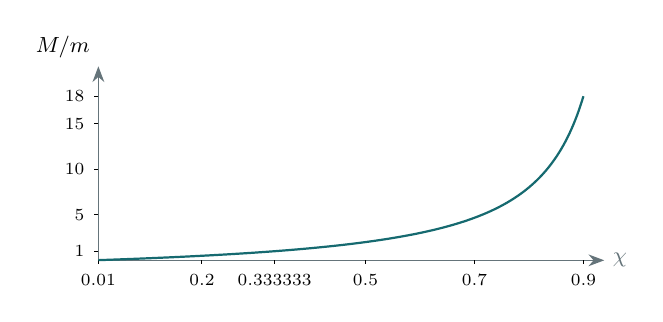
\begin{tikzpicture}[scale=.88,transform shape]
\draw[axis] (0,0.0)--(7.3,0.0) node[right] {$\chi$};
\draw[axis] (0,0)--(0,2.8);
\node[above left] at (0,2.8) {$M/m$};
\draw[thin] (0.000000,0.0)--(0.000000,-0.06);\node[below,font=\scriptsize] at (0.000000,-0.08) {$ 0.01 $};
\draw[thin] (1.494382,0.0)--(1.494382,-0.06);\node[below,font=\scriptsize] at (1.494382,-0.08) {$ 0.2 $};
\draw[thin] (2.543071,0.0)--(2.543071,-0.06);\node[below,font=\scriptsize] at (2.543071,-0.08) {$ 0.333333 $};
\draw[thin] (3.853933,0.0)--(3.853933,-0.06);\node[below,font=\scriptsize] at (3.853933,-0.08) {$ 0.5 $};
\draw[thin] (5.426966,0.0)--(5.426966,-0.06);\node[below,font=\scriptsize] at (5.426966,-0.08) {$ 0.7 $};
\draw[thin] (7.000000,0.0)--(7.000000,-0.06);\node[below,font=\scriptsize] at (7.000000,-0.08) {$ 0.9 $};
\draw[thin] (0,0.131579)--(-.06,0.131579);\node[left,font=\scriptsize] at (-.08,0.131579) {$ 1 $};
\draw[thin] (0,0.657895)--(-.06,0.657895);\node[left,font=\scriptsize] at (-.08,0.657895) {$ 5 $};
\draw[thin] (0,1.315789)--(-.06,1.315789);\node[left,font=\scriptsize] at (-.08,1.315789) {$ 10 $};
\draw[thin] (0,1.973684)--(-.06,1.973684);\node[left,font=\scriptsize] at (-.08,1.973684) {$ 15 $};
\draw[thin] (0,2.368421)--(-.06,2.368421);\node[left,font=\scriptsize] at (-.08,2.368421) {$ 18 $};
\draw[thick,color=accent] plot coordinates {(0.0000000,0.0026582) (0.0291667,0.0036576) (0.0583333,0.0046646) (0.0875000,0.0056792) (0.1166667,0.0067015) (0.1458333,0.0077316) (0.1750000,0.0087697) (0.2041667,0.0098157) (0.2333333,0.0108698) (0.2625000,0.0119320) (0.2916667,0.0130026) (0.3208333,0.0140814) (0.3500000,0.0151688) (0.3791667,0.0162647) (0.4083333,0.0173693) (0.4375000,0.0184827) (0.4666667,0.0196049) (0.4958333,0.0207361) (0.5250000,0.0218764) (0.5541667,0.0230259) (0.5833333,0.0241847) (0.6125000,0.0253529) (0.6416667,0.0265306) (0.6708333,0.0277181) (0.7000000,0.0289152) (0.7291667,0.0301223) (0.7583333,0.0313394) (0.7875000,0.0325667) (0.8166667,0.0338042) (0.8458333,0.0350521) (0.8750000,0.0363105) (0.9041667,0.0375797) (0.9333333,0.0388596) (0.9625000,0.0401504) (0.9916667,0.0414524) (1.0208333,0.0427655) (1.0500000,0.0440901) (1.0791667,0.0454261) (1.1083333,0.0467739) (1.1375000,0.0481334) (1.1666667,0.0495050) (1.1958333,0.0508886) (1.2250000,0.0522846) (1.2541667,0.0536930) (1.2833333,0.0551141) (1.3125000,0.0565480) (1.3416667,0.0579948) (1.3708333,0.0594548) (1.4000000,0.0609282) (1.4291667,0.0624150) (1.4583333,0.0639156) (1.4875000,0.0654301) (1.5166667,0.0669586) (1.5458333,0.0685015) (1.5750000,0.0700588) (1.6041667,0.0716308) (1.6333333,0.0732178) (1.6625000,0.0748198) (1.6916667,0.0764372) (1.7208333,0.0780701) (1.7500000,0.0797188) (1.7791667,0.0813836) (1.8083333,0.0830645) (1.8375000,0.0847620) (1.8666667,0.0864762) (1.8958333,0.0882073) (1.9250000,0.0899557) (1.9541667,0.0917215) (1.9833333,0.0935052) (2.0125000,0.0953068) (2.0416667,0.0971267) (2.0708333,0.0989652) (2.1000000,0.1008226) (2.1291667,0.1026991) (2.1583333,0.1045951) (2.1875000,0.1065108) (2.2166667,0.1084466) (2.2458333,0.1104027) (2.2750000,0.1123796) (2.3041667,0.1143775) (2.3333333,0.1163968) (2.3625000,0.1184377) (2.3916667,0.1205008) (2.4208333,0.1225863) (2.4500000,0.1246946) (2.4791667,0.1268260) (2.5083333,0.1289810) (2.5375000,0.1311600) (2.5666667,0.1333633) (2.5958333,0.1355914) (2.6250000,0.1378446) (2.6541667,0.1401235) (2.6833333,0.1424284) (2.7125000,0.1447598) (2.7416667,0.1471182) (2.7708333,0.1495039) (2.8000000,0.1519176) (2.8291667,0.1543598) (2.8583333,0.1568308) (2.8875000,0.1593312) (2.9166667,0.1618616) (2.9458333,0.1644225) (2.9750000,0.1670144) (3.0041667,0.1696379) (3.0333333,0.1722937) (3.0625000,0.1749822) (3.0916667,0.1777041) (3.1208333,0.1804601) (3.1500000,0.1832507) (3.1791667,0.1860767) (3.2083333,0.1889387) (3.2375000,0.1918374) (3.2666667,0.1947735) (3.2958333,0.1977477) (3.3250000,0.2007608) (3.3541667,0.2038136) (3.3833333,0.2069068) (3.4125000,0.2100413) (3.4416667,0.2132178) (3.4708333,0.2164373) (3.5000000,0.2197006) (3.5291667,0.2230086) (3.5583333,0.2263623) (3.5875000,0.2297625) (3.6166667,0.2332103) (3.6458333,0.2367067) (3.6750000,0.2402527) (3.7041667,0.2438494) (3.7333333,0.2474978) (3.7625000,0.2511991) (3.7916667,0.2549544) (3.8208333,0.2587650) (3.8500000,0.2626321) (3.8791667,0.2665569) (3.9083333,0.2705407) (3.9375000,0.2745849) (3.9666667,0.2786909) (3.9958333,0.2828600) (4.0250000,0.2870938) (4.0541667,0.2913938) (4.0833333,0.2957615) (4.1125000,0.3001986) (4.1416667,0.3047067) (4.1708333,0.3092874) (4.2000000,0.3139428) (4.2291667,0.3186744) (4.2583333,0.3234843) (4.2875000,0.3283743) (4.3166667,0.3333466) (4.3458333,0.3384032) (4.3750000,0.3435462) (4.4041667,0.3487779) (4.4333333,0.3541007) (4.4625000,0.3595168) (4.4916667,0.3650288) (4.5208333,0.3706393) (4.5500000,0.3763510) (4.5791667,0.3821665) (4.6083333,0.3880887) (4.6375000,0.3941206) (4.6666667,0.4002654) (4.6958333,0.4065261) (4.7250000,0.4129061) (4.7541667,0.4194088) (4.7833333,0.4260378) (4.8125000,0.4327969) (4.8416667,0.4396898) (4.8708333,0.4467207) (4.9000000,0.4538936) (4.9291667,0.4612130) (4.9583333,0.4686833) (4.9875000,0.4763093) (5.0166667,0.4840959) (5.0458333,0.4920483) (5.0750000,0.5001717) (5.1041667,0.5084719) (5.1333333,0.5169544) (5.1625000,0.5256256) (5.1916667,0.5344917) (5.2208333,0.5435594) (5.2500000,0.5528356) (5.2791667,0.5623276) (5.3083333,0.5720430) (5.3375000,0.5819899) (5.3666667,0.5921765) (5.3958333,0.6026117) (5.4250000,0.6133047) (5.4541667,0.6242651) (5.4833333,0.6355031) (5.5125000,0.6470294) (5.5416667,0.6588552) (5.5708333,0.6709923) (5.6000000,0.6834532) (5.6291667,0.6962511) (5.6583333,0.7093998) (5.6875000,0.7229138) (5.7166667,0.7368088) (5.7458333,0.7511009) (5.7750000,0.7658075) (5.8041667,0.7809468) (5.8333333,0.7965383) (5.8625000,0.8126025) (5.8916667,0.8291613) (5.9208333,0.8462378) (5.9500000,0.8638566) (5.9791667,0.8820442) (6.0083333,0.9008284) (6.0375000,0.9202390) (6.0666667,0.9403081) (6.0958333,0.9610696) (6.1250000,0.9825600) (6.1541667,1.0048183) (6.1833333,1.0278866) (6.2125000,1.0518097) (6.2416667,1.0766362) (6.2708333,1.1024182) (6.3000000,1.1292119) (6.3291667,1.1570781) (6.3583333,1.1860825) (6.3875000,1.2162962) (6.4166667,1.2477965) (6.4458333,1.2806674) (6.4750000,1.3150004) (6.5041667,1.3508951) (6.5333333,1.3884607) (6.5625000,1.4278165) (6.5916667,1.4690937) (6.6208333,1.5124366) (6.6500000,1.5580040) (6.6791667,1.6059719) (6.7083333,1.6565350) (6.7375000,1.7099097) (6.7666667,1.7663374) (6.7958333,1.8260877) (6.8250000,1.8894629) (6.8541667,1.9568033) (6.8833333,2.0284929) (6.9125000,2.1049671) (6.9416667,2.1867217) (6.9708333,2.2743228) (7.0000000,2.3684211)};
\end{tikzpicture}
\figcaption{变图力试1.3V8\quad 由地面路程分离的水平比例反演质量比}
\end{minipage}\end{center}
\end{enumerate}

\Needspace{13\baselineskip}

\pdfbookmark[2]{第 4 题 弹出小球与自由细杆端点再次相遇}{q4}

\section*{第 4 题\quad 弹出小球与自由细杆端点再次相遇}\label{q:4}


质量为$M$、长度为$l$的均匀细杆$AB$静止在光滑水平面上。$B$端的轻弹簧将质量为$m$的小球斜向弹出，弹出后小球的地面速度大小为$v$，与从$B$指向$A$的方向夹角为$\varphi$，$0<\varphi<\pi/2$。

要求小球自由运动后恰与杆的$A$端相遇，且相遇前细杆的转角不超过$\pi$。求质量比$\gamma=M/m$与发射角$\varphi$的关系及其允许范围。忽略球与杆的厚度、摩擦和弹簧质量，弹出后到再次相遇前球与杆无相互作用。


\begin{center}\begin{minipage}{.98\linewidth}\centering
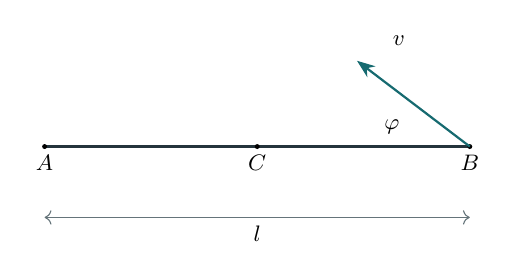
\begin{tikzpicture}[scale=.9,transform shape]
\draw[object] (-3.00000,0.00000)--(3.00000,0.00000);\fill (-3.00000,0.00000) circle(.035);\node[below] at (-3.00000,0.00000) {$A$};\fill (0.00000,0.00000) circle(.035);\node[below] at (0.00000,0.00000) {$C$};\fill (3.00000,0.00000) circle(.035);\node[below] at (3.00000,0.00000) {$B$};\draw[motion] (3.00000,0.00000)--(1.40783,1.21037);\node[above] at (2.00000,1.30000) {$v$};\node[above] at (1.90000,0.05000) {$\varphi$};\draw[<->,thin,color=muted] (-3.00000,-1.00000)--(3.00000,-1.00000);\node[below] at (0.00000,-1.00000) {$l$};
\end{tikzpicture}
\figcaption{图力试1.4\quad 斜向发射后，球和杆质心沿相反方向平移。}
\end{minipage}\end{center}

\Needspace{8\baselineskip}

\pdfbookmark[3]{题型定位}{q4-h0}

\subsection*{题型定位}

发射冲量决定自由杆的质心速度和自转角速率，在随杆质心匀速平移的惯性系中，将球的直线运动与杆端的圆弧运动配对。单调的正弦比函数给质量与发射角的一一对应。

\Needspace{8\baselineskip}

\pdfbookmark[3]{知识点}{q4-h1}

\subsection*{知识点}

\begin{itemize}
\item 球杆总水平动量守恒，端点冲量相对杆质心产生转动冲量。
\item 杆质心作匀速平移，球相对质心的速度为两者速度矢量之差。
\item 半径$l/2$圆中的弦长和圆周角给$\Theta=2\varphi$、弦长$l\cos\varphi$。
\item $\sin x/x$在$0<x<\pi$上严格下降，配对方程决定唯一角度。
\item 法向距离保持正值，说明球在目标端点相遇前自由离杆运动。\end{itemize}

\Needspace{8\baselineskip}

\pdfbookmark[3]{物理图像}{q4-h2}

\subsection*{物理图像}

A图随C平移而坐标轴固定，球从B沿弦到达圆周上的A端，杆在同一时间内顺时针转过两倍发射角。B图给质量与角度的单调关系，C图画碰撞前正的法向距离，D图显示地面系的球直线、杆质心直线与A端复合轨迹。

\Needspace{8\baselineskip}

\pdfbookmark[3]{解题入口}{q4-h3}

\subsection*{解题入口}

先把小球初速度写成地面二维分量，由反向冲量求杆质心速度与顺时针角速率。移到随C匀速平移的系，用相对速度和第二个圆周交点求弦长、杆转角，再以共同飞行时间连接平移与转动。

\Needspace{8\baselineskip}

\pdfbookmark[3]{标准解法}{q4-h4}

\subsection*{标准解法}


图力试1.4中，取初始杆质心$C$为坐标原点，$B=(l/2,0)$，$A=(-l/2,0)$。记$\gamma=M/m$。小球初速度为
\[
\boldsymbol v=v(-\cos\varphi,\sin\varphi).
\]
对冲量过程用水平动量守恒，细杆质心速度为
\[
\boldsymbol V_C=\frac{v}{\gamma}(\cos\varphi,-\sin\varphi).
\]
对细杆自身质心列转动冲量方程，端点$B$所受冲量与小球获得的冲量相反。杆的转动惯量$I_C=Ml^2/12$，故杆向顺时针转动，角速率
\[
I_C\Omega=\frac l2\,mv\sin\varphi,\qquad
\boxed{\Omega=\frac{6v\sin\varphi}{\gamma l}}.
\]
弹出后杆无水平力和竖直轴力矩，$\boldsymbol V_C,\Omega$均保持不变。

\begin{center}\begin{minipage}{.98\linewidth}\centering
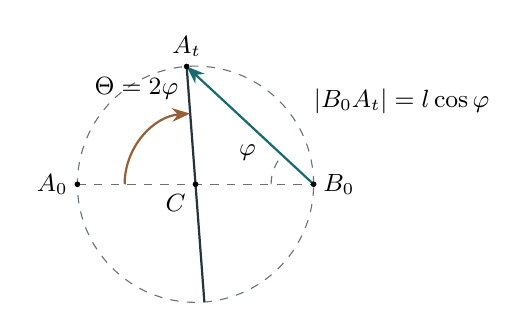
\begin{tikzpicture}[scale=3]
\draw[guide] (0,0) circle(.5);\draw[guide] (-.5,0)--(.5,0);
\draw[object] (-0.0374722,0.4985939)--(0.0374722,-0.4985939);
\draw[motion] (.5,0)--(-0.0374722,0.4985939);
\fill (.5,0) circle(.012) node[right] {$B_0$};\fill (-.5,0) circle(.012) node[left] {$A_0$};\fill (0,0) circle(.012) node[below left] {$C$};
\fill (-0.0374722,0.4985939) circle(.012) node[above] {$A_t$};
\draw[force] (-.3,0) arc(180:94.2980291:.3);
\draw[guide] (.32,0) arc(180:137.1490145:.18);
\node[above] at (-.25,.32) {$\Theta=2\varphi$};\node[above] at (.22,.06) {$\varphi$};
\node[right] at (.46,.35) {$|B_0A_t|=l\cos\varphi$};
\end{tikzpicture}
\figcaption{解图力试1.4A\quad 随C匀速平移的惯性系，球走弦而A端走短弧}
\end{minipage}\end{center}
解图力试1.4A在随$C$匀速平移、但坐标轴不转动的参考系中画图。小球相对速度是
\[
\boldsymbol w=\boldsymbol v-\boldsymbol V_C
=\left(1+\frac1\gamma\right)v(-\cos\varphi,\sin\varphi).
\]
于是小球从$B$沿直线行进，杆的$A$端沿半径$l/2$的圆周运动。设杆转过顺时针角$\Theta=\Omega t$。要求两者相遇，就要让该直线的第二个圆周交点恰好是此时的$A$端。

解图力试1.4A把弦$BA_t$与直径$BA$的夹角标为$\varphi$。相遇时
\[
A_t=\left(-\frac l2\cos\Theta,\frac l2\sin\Theta\right),
\qquad
A_t-B=\frac l2(-1-\cos\Theta,\sin\Theta).
\]
由两分量的比值，
\[
\tan\varphi=\frac{\sin\Theta}{1+\cos\Theta}
=\tan\frac{\Theta}{2}.
\]
在$0<\Theta\le\pi$的短弧分支中得到
\[
\Theta=2\varphi,\qquad |BA_t|=l\cos\varphi.
\]
弦长除以相对速率给相遇时间，故
\[
t=\frac{l\cos\varphi}{(1+1/\gamma)v},
\qquad
\Omega t=\frac{3\sin2\varphi}{1+\gamma}=2\varphi.
\]
因此所求配对关系是
\[
\boxed{\frac{1+\gamma}{3}=\frac{\sin2\varphi}{2\varphi}},
\qquad
\gamma=3\frac{\sin2\varphi}{2\varphi}-1.
\]
相遇条件只含质量比和几何角；提高发射速度会同时缩短球的飞行时间、加快杆的转动，两项在转角中抵消。

\begin{center}\begin{minipage}{.98\linewidth}\centering
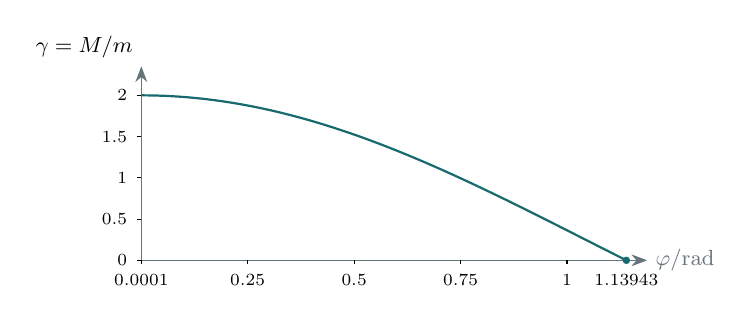
\begin{tikzpicture}[scale=.88,transform shape]
\draw[axis] (0,0.0)--(7.3,0.0) node[right] {$\varphi/\mathrm{rad}$};
\draw[axis] (0,0)--(0,2.8);
\node[above left] at (0,2.8) {$\gamma=M/m$};
\draw[thin] (0.000000,0.0)--(0.000000,-0.06);\node[below,font=\scriptsize] at (0.000000,-0.08) {$ 0.0001 $};
\draw[thin] (1.535374,0.0)--(1.535374,-0.06);\node[below,font=\scriptsize] at (1.535374,-0.08) {$ 0.25 $};
\draw[thin] (3.071363,0.0)--(3.071363,-0.06);\node[below,font=\scriptsize] at (3.071363,-0.08) {$ 0.5 $};
\draw[thin] (4.607352,0.0)--(4.607352,-0.06);\node[below,font=\scriptsize] at (4.607352,-0.08) {$ 0.75 $};
\draw[thin] (6.143340,0.0)--(6.143340,-0.06);\node[below,font=\scriptsize] at (6.143340,-0.08) {$ 1 $};
\draw[thin] (7.000000,0.0)--(7.000000,-0.06);\node[below,font=\scriptsize] at (7.000000,-0.08) {$ 1.13943 $};
\draw[thin] (0,0.000000)--(-.06,0.000000);\node[left,font=\scriptsize] at (-.08,0.000000) {$ 0 $};
\draw[thin] (0,0.595238)--(-.06,0.595238);\node[left,font=\scriptsize] at (-.08,0.595238) {$ 0.5 $};
\draw[thin] (0,1.190476)--(-.06,1.190476);\node[left,font=\scriptsize] at (-.08,1.190476) {$ 1 $};
\draw[thin] (0,1.785714)--(-.06,1.785714);\node[left,font=\scriptsize] at (-.08,1.785714) {$ 1.5 $};
\draw[thin] (0,2.380952)--(-.06,2.380952);\node[left,font=\scriptsize] at (-.08,2.380952) {$ 2 $};
\draw[thick,color=accent] plot coordinates {(0.0000000,2.3809524) (0.0291667,2.3808964) (0.0583333,2.3807332) (0.0875000,2.3804627) (0.1166667,2.3800849) (0.1458333,2.3795998) (0.1750000,2.3790075) (0.2041667,2.3783079) (0.2333333,2.3775012) (0.2625000,2.3765874) (0.2916667,2.3755665) (0.3208333,2.3744385) (0.3500000,2.3732036) (0.3791667,2.3718618) (0.4083333,2.3704132) (0.4375000,2.3688579) (0.4666667,2.3671959) (0.4958333,2.3654273) (0.5250000,2.3635522) (0.5541667,2.3615708) (0.5833333,2.3594831) (0.6125000,2.3572892) (0.6416667,2.3549893) (0.6708333,2.3525835) (0.7000000,2.3500720) (0.7291667,2.3474547) (0.7583333,2.3447320) (0.7875000,2.3419039) (0.8166667,2.3389706) (0.8458333,2.3359323) (0.8750000,2.3327891) (0.9041667,2.3295412) (0.9333333,2.3261887) (0.9625000,2.3227319) (0.9916667,2.3191709) (1.0208333,2.3155060) (1.0500000,2.3117372) (1.0791667,2.3078649) (1.1083333,2.3038892) (1.1375000,2.2998104) (1.1666667,2.2956287) (1.1958333,2.2913442) (1.2250000,2.2869573) (1.2541667,2.2824681) (1.2833333,2.2778769) (1.3125000,2.2731840) (1.3416667,2.2683896) (1.3708333,2.2634939) (1.4000000,2.2584973) (1.4291667,2.2534000) (1.4583333,2.2482022) (1.4875000,2.2429043) (1.5166667,2.2375065) (1.5458333,2.2320092) (1.5750000,2.2264126) (1.6041667,2.2207170) (1.6333333,2.2149227) (1.6625000,2.2090301) (1.6916667,2.2030394) (1.7208333,2.1969510) (1.7500000,2.1907652) (1.7791667,2.1844824) (1.8083333,2.1781028) (1.8375000,2.1716269) (1.8666667,2.1650549) (1.8958333,2.1583872) (1.9250000,2.1516243) (1.9541667,2.1447663) (1.9833333,2.1378138) (2.0125000,2.1307671) (2.0416667,2.1236265) (2.0708333,2.1163925) (2.1000000,2.1090654) (2.1291667,2.1016456) (2.1583333,2.0941336) (2.1875000,2.0865297) (2.2166667,2.0788343) (2.2458333,2.0710478) (2.2750000,2.0631708) (2.3041667,2.0552035) (2.3333333,2.0471464) (2.3625000,2.0389999) (2.3916667,2.0307646) (2.4208333,2.0224407) (2.4500000,2.0140288) (2.4791667,2.0055293) (2.5083333,1.9969427) (2.5375000,1.9882694) (2.5666667,1.9795099) (2.5958333,1.9706646) (2.6250000,1.9617341) (2.6541667,1.9527188) (2.6833333,1.9436191) (2.7125000,1.9344356) (2.7416667,1.9251688) (2.7708333,1.9158191) (2.8000000,1.9063871) (2.8291667,1.8968732) (2.8583333,1.8872779) (2.8875000,1.8776019) (2.9166667,1.8678455) (2.9458333,1.8580093) (2.9750000,1.8480938) (3.0041667,1.8380996) (3.0333333,1.8280271) (3.0625000,1.8178770) (3.0916667,1.8076497) (3.1208333,1.7973458) (3.1500000,1.7869658) (3.1791667,1.7765103) (3.2083333,1.7659799) (3.2375000,1.7553750) (3.2666667,1.7446963) (3.2958333,1.7339444) (3.3250000,1.7231197) (3.3541667,1.7122229) (3.3833333,1.7012545) (3.4125000,1.6902152) (3.4416667,1.6791054) (3.4708333,1.6679258) (3.5000000,1.6566770) (3.5291667,1.6453596) (3.5583333,1.6339741) (3.5875000,1.6225212) (3.6166667,1.6110015) (3.6458333,1.5994155) (3.6750000,1.5877639) (3.7041667,1.5760473) (3.7333333,1.5642663) (3.7625000,1.5524215) (3.7916667,1.5405136) (3.8208333,1.5285431) (3.8500000,1.5165108) (3.8791667,1.5044171) (3.9083333,1.4922628) (3.9375000,1.4800486) (3.9666667,1.4677749) (3.9958333,1.4554425) (4.0250000,1.4430521) (4.0541667,1.4306042) (4.0833333,1.4180995) (4.1125000,1.4055387) (4.1416667,1.3929224) (4.1708333,1.3802513) (4.2000000,1.3675260) (4.2291667,1.3547472) (4.2583333,1.3419156) (4.2875000,1.3290318) (4.3166667,1.3160965) (4.3458333,1.3031104) (4.3750000,1.2900741) (4.4041667,1.2769884) (4.4333333,1.2638538) (4.4625000,1.2506711) (4.4916667,1.2374410) (4.5208333,1.2241641) (4.5500000,1.2108411) (4.5791667,1.1974727) (4.6083333,1.1840597) (4.6375000,1.1706026) (4.6666667,1.1571022) (4.6958333,1.1435592) (4.7250000,1.1299743) (4.7541667,1.1163481) (4.7833333,1.1026815) (4.8125000,1.0889749) (4.8416667,1.0752293) (4.8708333,1.0614453) (4.9000000,1.0476235) (4.9291667,1.0337648) (4.9583333,1.0198697) (4.9875000,1.0059390) (5.0166667,0.9919735) (5.0458333,0.9779738) (5.0750000,0.9639407) (5.1041667,0.9498748) (5.1333333,0.9357769) (5.1625000,0.9216477) (5.1916667,0.9074879) (5.2208333,0.8932982) (5.2500000,0.8790794) (5.2791667,0.8648322) (5.3083333,0.8505572) (5.3375000,0.8362553) (5.3666667,0.8219271) (5.3958333,0.8075733) (5.4250000,0.7931947) (5.4541667,0.7787921) (5.4833333,0.7643660) (5.5125000,0.7499173) (5.5416667,0.7354467) (5.5708333,0.7209550) (5.6000000,0.7064427) (5.6291667,0.6919107) (5.6583333,0.6773597) (5.6875000,0.6627904) (5.7166667,0.6482035) (5.7458333,0.6335999) (5.7750000,0.6189801) (5.8041667,0.6043449) (5.8333333,0.5896951) (5.8625000,0.5750314) (5.8916667,0.5603545) (5.9208333,0.5456651) (5.9500000,0.5309640) (5.9791667,0.5162519) (6.0083333,0.5015294) (6.0375000,0.4867975) (6.0666667,0.4720567) (6.0958333,0.4573078) (6.1250000,0.4425515) (6.1541667,0.4277886) (6.1833333,0.4130198) (6.2125000,0.3982457) (6.2416667,0.3834671) (6.2708333,0.3686848) (6.3000000,0.3538995) (6.3291667,0.3391119) (6.3583333,0.3243226) (6.3875000,0.3095325) (6.4166667,0.2947422) (6.4458333,0.2799525) (6.4750000,0.2651640) (6.5041667,0.2503775) (6.5333333,0.2355938) (6.5625000,0.2208134) (6.5916667,0.2060372) (6.6208333,0.1912659) (6.6500000,0.1765001) (6.6791667,0.1617405) (6.7083333,0.1469879) (6.7375000,0.1322430) (6.7666667,0.1175065) (6.7958333,0.1027791) (6.8250000,0.0880614) (6.8541667,0.0733542) (6.8833333,0.0586582) (6.9125000,0.0439741) (6.9416667,0.0293026) (6.9708333,0.0146443) (7.0000000,-0.0000000)};
\draw[fill=white,color=accent] (7.0000000,-0.0000000) circle(.045);
\end{tikzpicture}
\figcaption{解图力试1.4B\quad 质量比与发射角的唯一配对，两个极限端点均不取}
\end{minipage}\end{center}
解图力试1.4B画出质量比随发射角的变化。为判断允许范围，令$x=2\varphi\in(0,\pi)$。函数$f(x)=\sin x/x$严格下降，因为
\[
f'(x)=\frac{x\cos x-\sin x}{x^2}<0;
\quad
\frac{\dd}{\dd x}(\sin x-x\cos x)=x\sin x>0.
\]
它从1降到0。再结合$\gamma>0$，得到
\[
\boxed{0<\gamma<2,\qquad 0<\varphi<\varphi_0},
\quad
\frac{\sin2\varphi_0}{2\varphi_0}=\frac13,
\quad \varphi_0\simeq1.1394\,\mathrm{rad}.
\]
对任意给定$0<\gamma<2$，有且只有一个允许发射角；质量比与角度通过上式一一配对，两个范围共同受同一等式约束。

同一相遇解还给出碰撞前球到杆身的法向距离。在$0<\Theta<2\varphi$时，小球位置为
\[
\boldsymbol r(\Theta)=\frac l2(1,0)
+\frac{l\Theta\cos\varphi}{2\varphi}
(-\cos\varphi,\sin\varphi).
\]
球到杆的有向直线的法向距离，乘$2/l$后为
\[
\frac{2}{l}\,\boldsymbol r(\Theta)\cdot
(\sin\Theta,\cos\Theta)
=\sin\Theta+
\frac{\Theta\cos\varphi}{\varphi}\sin(\varphi-\Theta)>0.
\]
在$0<\Theta\le\varphi$，两项均非负且第一项为正。在$\varphi<\Theta<2\varphi$，利用
\[
\frac{\sin\Theta}{\Theta}>
\frac{\sin2\varphi}{2\varphi}
=\frac{\cos\varphi\sin\varphi}{\varphi}
\ge\frac{\cos\varphi}{\varphi}\sin(\Theta-\varphi)
\]
也得严格正值。因此再次相交在$A_t$。解图力试1.4C画出相等质量时这段法向距离，开区间内为正，末端回到零。
\begin{center}\begin{minipage}{.98\linewidth}\centering
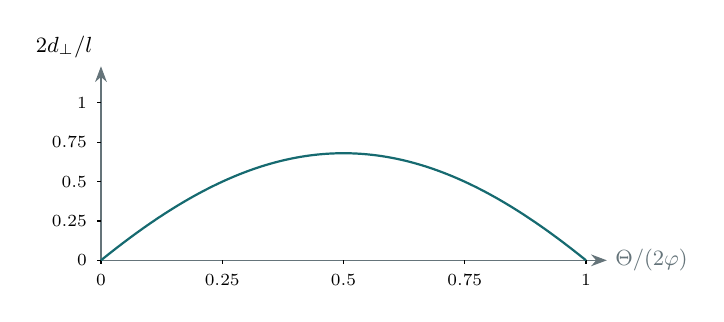
\begin{tikzpicture}[scale=.88,transform shape]
\draw[axis] (0,0.0)--(7.3,0.0) node[right] {$\Theta/(2\varphi)$};
\draw[axis] (0,0)--(0,2.8);
\node[above left] at (0,2.8) {$2d_\perp/l$};
\draw[thin] (0.000000,0.0)--(0.000000,-0.06);\node[below,font=\scriptsize] at (0.000000,-0.08) {$ 0 $};
\draw[thin] (1.750000,0.0)--(1.750000,-0.06);\node[below,font=\scriptsize] at (1.750000,-0.08) {$ 0.25 $};
\draw[thin] (3.500000,0.0)--(3.500000,-0.06);\node[below,font=\scriptsize] at (3.500000,-0.08) {$ 0.5 $};
\draw[thin] (5.250000,0.0)--(5.250000,-0.06);\node[below,font=\scriptsize] at (5.250000,-0.08) {$ 0.75 $};
\draw[thin] (7.000000,0.0)--(7.000000,-0.06);\node[below,font=\scriptsize] at (7.000000,-0.08) {$ 1 $};
\draw[thin] (0,0.000000)--(-.06,0.000000);\node[left,font=\scriptsize] at (-.08,0.000000) {$ 0 $};
\draw[thin] (0,0.568182)--(-.06,0.568182);\node[left,font=\scriptsize] at (-.08,0.568182) {$ 0.25 $};
\draw[thin] (0,1.136364)--(-.06,1.136364);\node[left,font=\scriptsize] at (-.08,1.136364) {$ 0.5 $};
\draw[thin] (0,1.704545)--(-.06,1.704545);\node[left,font=\scriptsize] at (-.08,1.704545) {$ 0.75 $};
\draw[thin] (0,2.272727)--(-.06,2.272727);\node[left,font=\scriptsize] at (-.08,2.272727) {$ 1 $};
\draw[thick,color=accent] plot coordinates {(0.0000000,0.0000000) (0.0291667,0.0235439) (0.0583333,0.0469594) (0.0875000,0.0702446) (0.1166667,0.0933981) (0.1458333,0.1164181) (0.1750000,0.1393032) (0.2041667,0.1620516) (0.2333333,0.1846619) (0.2625000,0.2071323) (0.2916667,0.2294615) (0.3208333,0.2516478) (0.3500000,0.2736896) (0.3791667,0.2955855) (0.4083333,0.3173339) (0.4375000,0.3389333) (0.4666667,0.3603823) (0.4958333,0.3816793) (0.5250000,0.4028228) (0.5541667,0.4238114) (0.5833333,0.4446437) (0.6125000,0.4653181) (0.6416667,0.4858334) (0.6708333,0.5061879) (0.7000000,0.5263804) (0.7291667,0.5464095) (0.7583333,0.5662737) (0.7875000,0.5859717) (0.8166667,0.6055022) (0.8458333,0.6248637) (0.8750000,0.6440550) (0.9041667,0.6630747) (0.9333333,0.6819216) (0.9625000,0.7005942) (0.9916667,0.7190914) (1.0208333,0.7374119) (1.0500000,0.7555544) (1.0791667,0.7735176) (1.1083333,0.7913004) (1.1375000,0.8089014) (1.1666667,0.8263196) (1.1958333,0.8435536) (1.2250000,0.8606024) (1.2541667,0.8774648) (1.2833333,0.8941395) (1.3125000,0.9106255) (1.3416667,0.9269216) (1.3708333,0.9430267) (1.4000000,0.9589397) (1.4291667,0.9746595) (1.4583333,0.9901851) (1.4875000,1.0055153) (1.5166667,1.0206492) (1.5458333,1.0355856) (1.5750000,1.0503237) (1.6041667,1.0648623) (1.6333333,1.0792004) (1.6625000,1.0933372) (1.6916667,1.1072716) (1.7208333,1.1210027) (1.7500000,1.1345295) (1.7791667,1.1478511) (1.8083333,1.1609667) (1.8375000,1.1738753) (1.8666667,1.1865760) (1.8958333,1.1990679) (1.9250000,1.2113503) (1.9541667,1.2234223) (1.9833333,1.2352831) (2.0125000,1.2469318) (2.0416667,1.2583676) (2.0708333,1.2695899) (2.1000000,1.2805977) (2.1291667,1.2913905) (2.1583333,1.3019673) (2.1875000,1.3123276) (2.2166667,1.3224706) (2.2458333,1.3323957) (2.2750000,1.3421021) (2.3041667,1.3515892) (2.3333333,1.3608563) (2.3625000,1.3699028) (2.3916667,1.3787282) (2.4208333,1.3873317) (2.4500000,1.3957129) (2.4791667,1.4038711) (2.5083333,1.4118058) (2.5375000,1.4195165) (2.5666667,1.4270027) (2.5958333,1.4342637) (2.6250000,1.4412992) (2.6541667,1.4481086) (2.6833333,1.4546916) (2.7125000,1.4610476) (2.7416667,1.4671762) (2.7708333,1.4730770) (2.8000000,1.4787496) (2.8291667,1.4841937) (2.8583333,1.4894088) (2.8875000,1.4943946) (2.9166667,1.4991507) (2.9458333,1.5036769) (2.9750000,1.5079729) (3.0041667,1.5120382) (3.0333333,1.5158728) (3.0625000,1.5194762) (3.0916667,1.5228483) (3.1208333,1.5259889) (3.1500000,1.5288976) (3.1791667,1.5315744) (3.2083333,1.5340190) (3.2375000,1.5362313) (3.2666667,1.5382112) (3.2958333,1.5399584) (3.3250000,1.5414729) (3.3541667,1.5427546) (3.3833333,1.5438034) (3.4125000,1.5446191) (3.4416667,1.5452019) (3.4708333,1.5455515) (3.5000000,1.5456681) (3.5291667,1.5455515) (3.5583333,1.5452019) (3.5875000,1.5446191) (3.6166667,1.5438034) (3.6458333,1.5427546) (3.6750000,1.5414729) (3.7041667,1.5399584) (3.7333333,1.5382112) (3.7625000,1.5362313) (3.7916667,1.5340190) (3.8208333,1.5315744) (3.8500000,1.5288976) (3.8791667,1.5259889) (3.9083333,1.5228483) (3.9375000,1.5194762) (3.9666667,1.5158728) (3.9958333,1.5120382) (4.0250000,1.5079729) (4.0541667,1.5036769) (4.0833333,1.4991507) (4.1125000,1.4943946) (4.1416667,1.4894088) (4.1708333,1.4841937) (4.2000000,1.4787496) (4.2291667,1.4730770) (4.2583333,1.4671762) (4.2875000,1.4610476) (4.3166667,1.4546916) (4.3458333,1.4481086) (4.3750000,1.4412992) (4.4041667,1.4342637) (4.4333333,1.4270027) (4.4625000,1.4195165) (4.4916667,1.4118058) (4.5208333,1.4038711) (4.5500000,1.3957129) (4.5791667,1.3873317) (4.6083333,1.3787282) (4.6375000,1.3699028) (4.6666667,1.3608563) (4.6958333,1.3515892) (4.7250000,1.3421021) (4.7541667,1.3323957) (4.7833333,1.3224706) (4.8125000,1.3123276) (4.8416667,1.3019673) (4.8708333,1.2913905) (4.9000000,1.2805977) (4.9291667,1.2695899) (4.9583333,1.2583676) (4.9875000,1.2469318) (5.0166667,1.2352831) (5.0458333,1.2234223) (5.0750000,1.2113503) (5.1041667,1.1990679) (5.1333333,1.1865760) (5.1625000,1.1738753) (5.1916667,1.1609667) (5.2208333,1.1478511) (5.2500000,1.1345295) (5.2791667,1.1210027) (5.3083333,1.1072716) (5.3375000,1.0933372) (5.3666667,1.0792004) (5.3958333,1.0648623) (5.4250000,1.0503237) (5.4541667,1.0355856) (5.4833333,1.0206492) (5.5125000,1.0055153) (5.5416667,0.9901851) (5.5708333,0.9746595) (5.6000000,0.9589397) (5.6291667,0.9430267) (5.6583333,0.9269216) (5.6875000,0.9106255) (5.7166667,0.8941395) (5.7458333,0.8774648) (5.7750000,0.8606024) (5.8041667,0.8435536) (5.8333333,0.8263196) (5.8625000,0.8089014) (5.8916667,0.7913004) (5.9208333,0.7735176) (5.9500000,0.7555544) (5.9791667,0.7374119) (6.0083333,0.7190914) (6.0375000,0.7005942) (6.0666667,0.6819216) (6.0958333,0.6630747) (6.1250000,0.6440550) (6.1541667,0.6248637) (6.1833333,0.6055022) (6.2125000,0.5859717) (6.2416667,0.5662737) (6.2708333,0.5464095) (6.3000000,0.5263804) (6.3291667,0.5061879) (6.3583333,0.4858334) (6.3875000,0.4653181) (6.4166667,0.4446437) (6.4458333,0.4238114) (6.4750000,0.4028228) (6.5041667,0.3816793) (6.5333333,0.3603823) (6.5625000,0.3389333) (6.5916667,0.3173339) (6.6208333,0.2955855) (6.6500000,0.2736896) (6.6791667,0.2516478) (6.7083333,0.2294615) (6.7375000,0.2071323) (6.7666667,0.1846619) (6.7958333,0.1620516) (6.8250000,0.1393032) (6.8541667,0.1164181) (6.8833333,0.0933981) (6.9125000,0.0702446) (6.9416667,0.0469594) (6.9708333,0.0235439) (7.0000000,-0.0000000)};
\end{tikzpicture}
\figcaption{解图力试1.4C\quad 相等质量时球到杆直线的有向法向距离}
\end{minipage}\end{center}
解图力试1.4D将同一相遇放回地面系，球走直线，杆质心沿反方向走直线，A端同时绕质心转动；两条地面轨迹在相遇时刻汇合。
\begin{center}\begin{minipage}{.98\linewidth}\centering
\begin{tikzpicture}[scale=4]
\draw[axis] (-.6,0)--(.7,0) node[right] {$x/l$};\draw[axis] (0,-.8)--(0,.45) node[above] {$y/l$};
\draw[thick,color=accent] plot coordinates {(0.5000000,0.0000000) (0.4988803,0.0010387) (0.4977605,0.0020775) (0.4966408,0.0031162) (0.4955211,0.0041549) (0.4944013,0.0051937) (0.4932816,0.0062324) (0.4921619,0.0072712) (0.4910421,0.0083099) (0.4899224,0.0093486) (0.4888027,0.0103874) (0.4876829,0.0114261) (0.4865632,0.0124648) (0.4854435,0.0135036) (0.4843237,0.0145423) (0.4832040,0.0155811) (0.4820843,0.0166198) (0.4809645,0.0176585) (0.4798448,0.0186973) (0.4787251,0.0197360) (0.4776053,0.0207747) (0.4764856,0.0218135) (0.4753659,0.0228522) (0.4742461,0.0238910) (0.4731264,0.0249297) (0.4720067,0.0259684) (0.4708869,0.0270072) (0.4697672,0.0280459) (0.4686475,0.0290846) (0.4675277,0.0301234) (0.4664080,0.0311621) (0.4652883,0.0322009) (0.4641685,0.0332396) (0.4630488,0.0342783) (0.4619291,0.0353171) (0.4608093,0.0363558) (0.4596896,0.0373945) (0.4585699,0.0384333) (0.4574501,0.0394720) (0.4563304,0.0405108) (0.4552106,0.0415495) (0.4540909,0.0425882) (0.4529712,0.0436270) (0.4518514,0.0446657) (0.4507317,0.0457044) (0.4496120,0.0467432) (0.4484922,0.0477819) (0.4473725,0.0488206) (0.4462528,0.0498594) (0.4451330,0.0508981) (0.4440133,0.0519369) (0.4428936,0.0529756) (0.4417738,0.0540143) (0.4406541,0.0550531) (0.4395344,0.0560918) (0.4384146,0.0571305) (0.4372949,0.0581693) (0.4361752,0.0592080) (0.4350554,0.0602468) (0.4339357,0.0612855) (0.4328160,0.0623242) (0.4316962,0.0633630) (0.4305765,0.0644017) (0.4294568,0.0654404) (0.4283370,0.0664792) (0.4272173,0.0675179) (0.4260976,0.0685567) (0.4249778,0.0695954) (0.4238581,0.0706341) (0.4227384,0.0716729) (0.4216186,0.0727116) (0.4204989,0.0737503) (0.4193792,0.0747891) (0.4182594,0.0758278) (0.4171397,0.0768666) (0.4160200,0.0779053) (0.4149002,0.0789440) (0.4137805,0.0799828) (0.4126608,0.0810215) (0.4115410,0.0820602) (0.4104213,0.0830990) (0.4093016,0.0841377) (0.4081818,0.0851765) (0.4070621,0.0862152) (0.4059424,0.0872539) (0.4048226,0.0882927) (0.4037029,0.0893314) (0.4025832,0.0903701) (0.4014634,0.0914089) (0.4003437,0.0924476) (0.3992240,0.0934863) (0.3981042,0.0945251) (0.3969845,0.0955638) (0.3958648,0.0966026) (0.3947450,0.0976413) (0.3936253,0.0986800) (0.3925056,0.0997188) (0.3913858,0.1007575) (0.3902661,0.1017962) (0.3891464,0.1028350) (0.3880266,0.1038737) (0.3869069,0.1049125) (0.3857872,0.1059512) (0.3846674,0.1069899) (0.3835477,0.1080287) (0.3824280,0.1090674) (0.3813082,0.1101061) (0.3801885,0.1111449) (0.3790688,0.1121836) (0.3779490,0.1132224) (0.3768293,0.1142611) (0.3757096,0.1152998) (0.3745898,0.1163386) (0.3734701,0.1173773) (0.3723503,0.1184160) (0.3712306,0.1194548) (0.3701109,0.1204935) (0.3689911,0.1215323) (0.3678714,0.1225710) (0.3667517,0.1236097) (0.3656319,0.1246485) (0.3645122,0.1256872) (0.3633925,0.1267259) (0.3622727,0.1277647) (0.3611530,0.1288034) (0.3600333,0.1298422) (0.3589135,0.1308809) (0.3577938,0.1319196) (0.3566741,0.1329584) (0.3555543,0.1339971) (0.3544346,0.1350358) (0.3533149,0.1360746) (0.3521951,0.1371133) (0.3510754,0.1381520) (0.3499557,0.1391908) (0.3488359,0.1402295) (0.3477162,0.1412683) (0.3465965,0.1423070) (0.3454767,0.1433457) (0.3443570,0.1443845) (0.3432373,0.1454232) (0.3421175,0.1464619) (0.3409978,0.1475007) (0.3398781,0.1485394) (0.3387583,0.1495782) (0.3376386,0.1506169) (0.3365189,0.1516556) (0.3353991,0.1526944) (0.3342794,0.1537331) (0.3331597,0.1547718) (0.3320399,0.1558106) (0.3309202,0.1568493) (0.3298005,0.1578881) (0.3286807,0.1589268) (0.3275610,0.1599655) (0.3264413,0.1610043) (0.3253215,0.1620430) (0.3242018,0.1630817) (0.3230821,0.1641205) (0.3219623,0.1651592) (0.3208426,0.1661980) (0.3197229,0.1672367) (0.3186031,0.1682754) (0.3174834,0.1693142) (0.3163637,0.1703529) (0.3152439,0.1713916) (0.3141242,0.1724304) (0.3130045,0.1734691) (0.3118847,0.1745078) (0.3107650,0.1755466) (0.3096453,0.1765853) (0.3085255,0.1776241) (0.3074058,0.1786628) (0.3062861,0.1797015) (0.3051663,0.1807403) (0.3040466,0.1817790) (0.3029269,0.1828177) (0.3018071,0.1838565) (0.3006874,0.1848952) (0.2995677,0.1859340) (0.2984479,0.1869727) (0.2973282,0.1880114) (0.2962085,0.1890502) (0.2950887,0.1900889) (0.2939690,0.1911276) (0.2928493,0.1921664) (0.2917295,0.1932051) (0.2906098,0.1942439) (0.2894901,0.1952826) (0.2883703,0.1963213) (0.2872506,0.1973601) (0.2861308,0.1983988) (0.2850111,0.1994375) (0.2838914,0.2004763) (0.2827716,0.2015150) (0.2816519,0.2025538) (0.2805322,0.2035925) (0.2794124,0.2046312) (0.2782927,0.2056700) (0.2771730,0.2067087) (0.2760532,0.2077474) (0.2749335,0.2087862) (0.2738138,0.2098249) (0.2726940,0.2108637) (0.2715743,0.2119024) (0.2704546,0.2129411) (0.2693348,0.2139799) (0.2682151,0.2150186) (0.2670954,0.2160573) (0.2659756,0.2170961) (0.2648559,0.2181348) (0.2637362,0.2191735) (0.2626164,0.2202123) (0.2614967,0.2212510) (0.2603770,0.2222898) (0.2592572,0.2233285) (0.2581375,0.2243672) (0.2570178,0.2254060) (0.2558980,0.2264447) (0.2547783,0.2274834) (0.2536586,0.2285222) (0.2525388,0.2295609) (0.2514191,0.2305997) (0.2502994,0.2316384) (0.2491796,0.2326771) (0.2480599,0.2337159) (0.2469402,0.2347546) (0.2458204,0.2357933) (0.2447007,0.2368321) (0.2435810,0.2378708) (0.2424612,0.2389096) (0.2413415,0.2399483) (0.2402218,0.2409870) (0.2391020,0.2420258) (0.2379823,0.2430645) (0.2368626,0.2441032) (0.2357428,0.2451420) (0.2346231,0.2461807) (0.2335034,0.2472195) (0.2323836,0.2482582) (0.2312639,0.2492969)};
\draw[thick,dashed,color=warm] plot coordinates {(-0.5000000,0.0000000) (-0.4988706,0.0020775) (-0.4977217,0.0041548) (-0.4965534,0.0062319) (-0.4953657,0.0083086) (-0.4941586,0.0103849) (-0.4929321,0.0124605) (-0.4916861,0.0145354) (-0.4904208,0.0166095) (-0.4891360,0.0186826) (-0.4878319,0.0207546) (-0.4865084,0.0228254) (-0.4851655,0.0248948) (-0.4838032,0.0269629) (-0.4824216,0.0290293) (-0.4810207,0.0310941) (-0.4796004,0.0331570) (-0.4781607,0.0352180) (-0.4767018,0.0372770) (-0.4752236,0.0393337) (-0.4737260,0.0413882) (-0.4722092,0.0434403) (-0.4706732,0.0454898) (-0.4691179,0.0475367) (-0.4675434,0.0495808) (-0.4659497,0.0516220) (-0.4643368,0.0536602) (-0.4627047,0.0556953) (-0.4610535,0.0577271) (-0.4593832,0.0597555) (-0.4576937,0.0617805) (-0.4559852,0.0638018) (-0.4542576,0.0658194) (-0.4525110,0.0678332) (-0.4507453,0.0698430) (-0.4489607,0.0718487) (-0.4471571,0.0738502) (-0.4453346,0.0758474) (-0.4434932,0.0778401) (-0.4416329,0.0798283) (-0.4397537,0.0818119) (-0.4378557,0.0837906) (-0.4359390,0.0857644) (-0.4340034,0.0877332) (-0.4320492,0.0896968) (-0.4300762,0.0916552) (-0.4280846,0.0936082) (-0.4260744,0.0955558) (-0.4240455,0.0974977) (-0.4219981,0.0994339) (-0.4199322,0.1013642) (-0.4178478,0.1032886) (-0.4157449,0.1052069) (-0.4136237,0.1071191) (-0.4114840,0.1090249) (-0.4093261,0.1109243) (-0.4071498,0.1128172) (-0.4049553,0.1147035) (-0.4027426,0.1165830) (-0.4005117,0.1184556) (-0.3982627,0.1203213) (-0.3959956,0.1221798) (-0.3937104,0.1240312) (-0.3914073,0.1258752) (-0.3890863,0.1277118) (-0.3867473,0.1295409) (-0.3843905,0.1313623) (-0.3820159,0.1331759) (-0.3796236,0.1349817) (-0.3772135,0.1367794) (-0.3747858,0.1385691) (-0.3723405,0.1403506) (-0.3698776,0.1421237) (-0.3673972,0.1438885) (-0.3648994,0.1456447) (-0.3623842,0.1473922) (-0.3598517,0.1491310) (-0.3573018,0.1508610) (-0.3547348,0.1525819) (-0.3521506,0.1542938) (-0.3495492,0.1559966) (-0.3469308,0.1576900) (-0.3442954,0.1593740) (-0.3416431,0.1610486) (-0.3389739,0.1627135) (-0.3362878,0.1643687) (-0.3335850,0.1660141) (-0.3308655,0.1676496) (-0.3281294,0.1692751) (-0.3253767,0.1708904) (-0.3226075,0.1724956) (-0.3198218,0.1740904) (-0.3170198,0.1756747) (-0.3142014,0.1772485) (-0.3113668,0.1788117) (-0.3085161,0.1803641) (-0.3056492,0.1819057) (-0.3027662,0.1834364) (-0.2998673,0.1849560) (-0.2969524,0.1864645) (-0.2940218,0.1879618) (-0.2910753,0.1894477) (-0.2881132,0.1909221) (-0.2851354,0.1923851) (-0.2821421,0.1938364) (-0.2791332,0.1952760) (-0.2761090,0.1967038) (-0.2730695,0.1981196) (-0.2700146,0.1995235) (-0.2669446,0.2009152) (-0.2638595,0.2022947) (-0.2607594,0.2036620) (-0.2576443,0.2050168) (-0.2545143,0.2063592) (-0.2513695,0.2076890) (-0.2482100,0.2090061) (-0.2450359,0.2103105) (-0.2418471,0.2116020) (-0.2386439,0.2128805) (-0.2354263,0.2141461) (-0.2321944,0.2153985) (-0.2289483,0.2166377) (-0.2256880,0.2178636) (-0.2224136,0.2190762) (-0.2191252,0.2202752) (-0.2158229,0.2214607) (-0.2125068,0.2226326) (-0.2091770,0.2237907) (-0.2058335,0.2249350) (-0.2024765,0.2260654) (-0.1991060,0.2271819) (-0.1957220,0.2282842) (-0.1923248,0.2293724) (-0.1889144,0.2304464) (-0.1854909,0.2315060) (-0.1820543,0.2325513) (-0.1786048,0.2335820) (-0.1751424,0.2345983) (-0.1716673,0.2355998) (-0.1681795,0.2365867) (-0.1646791,0.2375587) (-0.1611662,0.2385159) (-0.1576410,0.2394581) (-0.1541034,0.2403853) (-0.1505536,0.2412974) (-0.1469918,0.2421943) (-0.1434179,0.2430759) (-0.1398321,0.2439422) (-0.1362344,0.2447931) (-0.1326251,0.2456286) (-0.1290041,0.2464484) (-0.1253715,0.2472527) (-0.1217276,0.2480412) (-0.1180723,0.2488140) (-0.1144057,0.2495709) (-0.1107280,0.2503120) (-0.1070393,0.2510370) (-0.1033396,0.2517460) (-0.0996291,0.2524389) (-0.0959078,0.2531157) (-0.0921759,0.2537761) (-0.0884335,0.2544203) (-0.0846806,0.2550481) (-0.0809174,0.2556594) (-0.0771439,0.2562542) (-0.0733603,0.2568325) (-0.0695667,0.2573941) (-0.0657632,0.2579391) (-0.0619499,0.2584672) (-0.0581268,0.2589786) (-0.0542941,0.2594731) (-0.0504520,0.2599506) (-0.0466004,0.2604111) (-0.0427396,0.2608546) (-0.0388695,0.2612810) (-0.0349904,0.2616902) (-0.0311023,0.2620822) (-0.0272054,0.2624569) (-0.0232997,0.2628143) (-0.0193853,0.2631542) (-0.0154624,0.2634768) (-0.0115311,0.2637818) (-0.0075914,0.2640693) (-0.0036436,0.2643392) (0.0003124,0.2645914) (0.0042763,0.2648259) (0.0082481,0.2650427) (0.0122277,0.2652417) (0.0162150,0.2654228) (0.0202098,0.2655860) (0.0242120,0.2657313) (0.0282216,0.2658586) (0.0322383,0.2659679) (0.0362622,0.2660591) (0.0402931,0.2661322) (0.0443308,0.2661871) (0.0483753,0.2662238) (0.0524264,0.2662422) (0.0564841,0.2662424) (0.0605482,0.2662242) (0.0646185,0.2661877) (0.0686951,0.2661328) (0.0727778,0.2660594) (0.0768664,0.2659675) (0.0809608,0.2658571) (0.0850610,0.2657281) (0.0891668,0.2655806) (0.0932781,0.2654144) (0.0973947,0.2652296) (0.1015167,0.2650260) (0.1056437,0.2648038) (0.1097759,0.2645627) (0.1139129,0.2643029) (0.1180547,0.2640243) (0.1222012,0.2637268) (0.1263522,0.2634105) (0.1305077,0.2630752) (0.1346676,0.2627210) (0.1388316,0.2623478) (0.1429997,0.2619557) (0.1471718,0.2615445) (0.1513477,0.2611143) (0.1555274,0.2606651) (0.1597107,0.2601968) (0.1638975,0.2597093) (0.1680877,0.2592028) (0.1722811,0.2586770) (0.1764776,0.2581322) (0.1806772,0.2575681) (0.1848797,0.2569848) (0.1890849,0.2563824) (0.1932929,0.2557606) (0.1975033,0.2551196) (0.2017162,0.2544594) (0.2059313,0.2537799) (0.2101487,0.2530810) (0.2143681,0.2523629) (0.2185894,0.2516254) (0.2228126,0.2508686) (0.2270375,0.2500924) (0.2312639,0.2492969)};
\draw[thin,densely dotted,color=muted] plot coordinates {(0.0000000,-0.0000000) (0.0011197,-0.0010387) (0.0022395,-0.0020775) (0.0033592,-0.0031162) (0.0044789,-0.0041549) (0.0055987,-0.0051937) (0.0067184,-0.0062324) (0.0078381,-0.0072712) (0.0089579,-0.0083099) (0.0100776,-0.0093486) (0.0111973,-0.0103874) (0.0123171,-0.0114261) (0.0134368,-0.0124648) (0.0145565,-0.0135036) (0.0156763,-0.0145423) (0.0167960,-0.0155811) (0.0179157,-0.0166198) (0.0190355,-0.0176585) (0.0201552,-0.0186973) (0.0212749,-0.0197360) (0.0223947,-0.0207747) (0.0235144,-0.0218135) (0.0246341,-0.0228522) (0.0257539,-0.0238910) (0.0268736,-0.0249297) (0.0279933,-0.0259684) (0.0291131,-0.0270072) (0.0302328,-0.0280459) (0.0313525,-0.0290846) (0.0324723,-0.0301234) (0.0335920,-0.0311621) (0.0347117,-0.0322009) (0.0358315,-0.0332396) (0.0369512,-0.0342783) (0.0380709,-0.0353171) (0.0391907,-0.0363558) (0.0403104,-0.0373945) (0.0414301,-0.0384333) (0.0425499,-0.0394720) (0.0436696,-0.0405108) (0.0447894,-0.0415495) (0.0459091,-0.0425882) (0.0470288,-0.0436270) (0.0481486,-0.0446657) (0.0492683,-0.0457044) (0.0503880,-0.0467432) (0.0515078,-0.0477819) (0.0526275,-0.0488206) (0.0537472,-0.0498594) (0.0548670,-0.0508981) (0.0559867,-0.0519369) (0.0571064,-0.0529756) (0.0582262,-0.0540143) (0.0593459,-0.0550531) (0.0604656,-0.0560918) (0.0615854,-0.0571305) (0.0627051,-0.0581693) (0.0638248,-0.0592080) (0.0649446,-0.0602468) (0.0660643,-0.0612855) (0.0671840,-0.0623242) (0.0683038,-0.0633630) (0.0694235,-0.0644017) (0.0705432,-0.0654404) (0.0716630,-0.0664792) (0.0727827,-0.0675179) (0.0739024,-0.0685567) (0.0750222,-0.0695954) (0.0761419,-0.0706341) (0.0772616,-0.0716729) (0.0783814,-0.0727116) (0.0795011,-0.0737503) (0.0806208,-0.0747891) (0.0817406,-0.0758278) (0.0828603,-0.0768666) (0.0839800,-0.0779053) (0.0850998,-0.0789440) (0.0862195,-0.0799828) (0.0873392,-0.0810215) (0.0884590,-0.0820602) (0.0895787,-0.0830990) (0.0906984,-0.0841377) (0.0918182,-0.0851765) (0.0929379,-0.0862152) (0.0940576,-0.0872539) (0.0951774,-0.0882927) (0.0962971,-0.0893314) (0.0974168,-0.0903701) (0.0985366,-0.0914089) (0.0996563,-0.0924476) (0.1007760,-0.0934863) (0.1018958,-0.0945251) (0.1030155,-0.0955638) (0.1041352,-0.0966026) (0.1052550,-0.0976413) (0.1063747,-0.0986800) (0.1074944,-0.0997188) (0.1086142,-0.1007575) (0.1097339,-0.1017962) (0.1108536,-0.1028350) (0.1119734,-0.1038737) (0.1130931,-0.1049125) (0.1142128,-0.1059512) (0.1153326,-0.1069899) (0.1164523,-0.1080287) (0.1175720,-0.1090674) (0.1186918,-0.1101061) (0.1198115,-0.1111449) (0.1209312,-0.1121836) (0.1220510,-0.1132224) (0.1231707,-0.1142611) (0.1242904,-0.1152998) (0.1254102,-0.1163386) (0.1265299,-0.1173773) (0.1276497,-0.1184160) (0.1287694,-0.1194548) (0.1298891,-0.1204935) (0.1310089,-0.1215323) (0.1321286,-0.1225710) (0.1332483,-0.1236097) (0.1343681,-0.1246485) (0.1354878,-0.1256872) (0.1366075,-0.1267259) (0.1377273,-0.1277647) (0.1388470,-0.1288034) (0.1399667,-0.1298422) (0.1410865,-0.1308809) (0.1422062,-0.1319196) (0.1433259,-0.1329584) (0.1444457,-0.1339971) (0.1455654,-0.1350358) (0.1466851,-0.1360746) (0.1478049,-0.1371133) (0.1489246,-0.1381520) (0.1500443,-0.1391908) (0.1511641,-0.1402295) (0.1522838,-0.1412683) (0.1534035,-0.1423070) (0.1545233,-0.1433457) (0.1556430,-0.1443845) (0.1567627,-0.1454232) (0.1578825,-0.1464619) (0.1590022,-0.1475007) (0.1601219,-0.1485394) (0.1612417,-0.1495782) (0.1623614,-0.1506169) (0.1634811,-0.1516556) (0.1646009,-0.1526944) (0.1657206,-0.1537331) (0.1668403,-0.1547718) (0.1679601,-0.1558106) (0.1690798,-0.1568493) (0.1701995,-0.1578881) (0.1713193,-0.1589268) (0.1724390,-0.1599655) (0.1735587,-0.1610043) (0.1746785,-0.1620430) (0.1757982,-0.1630817) (0.1769179,-0.1641205) (0.1780377,-0.1651592) (0.1791574,-0.1661980) (0.1802771,-0.1672367) (0.1813969,-0.1682754) (0.1825166,-0.1693142) (0.1836363,-0.1703529) (0.1847561,-0.1713916) (0.1858758,-0.1724304) (0.1869955,-0.1734691) (0.1881153,-0.1745078) (0.1892350,-0.1755466) (0.1903547,-0.1765853) (0.1914745,-0.1776241) (0.1925942,-0.1786628) (0.1937139,-0.1797015) (0.1948337,-0.1807403) (0.1959534,-0.1817790) (0.1970731,-0.1828177) (0.1981929,-0.1838565) (0.1993126,-0.1848952) (0.2004323,-0.1859340) (0.2015521,-0.1869727) (0.2026718,-0.1880114) (0.2037915,-0.1890502) (0.2049113,-0.1900889) (0.2060310,-0.1911276) (0.2071507,-0.1921664) (0.2082705,-0.1932051) (0.2093902,-0.1942439) (0.2105099,-0.1952826) (0.2116297,-0.1963213) (0.2127494,-0.1973601) (0.2138692,-0.1983988) (0.2149889,-0.1994375) (0.2161086,-0.2004763) (0.2172284,-0.2015150) (0.2183481,-0.2025538) (0.2194678,-0.2035925) (0.2205876,-0.2046312) (0.2217073,-0.2056700) (0.2228270,-0.2067087) (0.2239468,-0.2077474) (0.2250665,-0.2087862) (0.2261862,-0.2098249) (0.2273060,-0.2108637) (0.2284257,-0.2119024) (0.2295454,-0.2129411) (0.2306652,-0.2139799) (0.2317849,-0.2150186) (0.2329046,-0.2160573) (0.2340244,-0.2170961) (0.2351441,-0.2181348) (0.2362638,-0.2191735) (0.2373836,-0.2202123) (0.2385033,-0.2212510) (0.2396230,-0.2222898) (0.2407428,-0.2233285) (0.2418625,-0.2243672) (0.2429822,-0.2254060) (0.2441020,-0.2264447) (0.2452217,-0.2274834) (0.2463414,-0.2285222) (0.2474612,-0.2295609) (0.2485809,-0.2305997) (0.2497006,-0.2316384) (0.2508204,-0.2326771) (0.2519401,-0.2337159) (0.2530598,-0.2347546) (0.2541796,-0.2357933) (0.2552993,-0.2368321) (0.2564190,-0.2378708) (0.2575388,-0.2389096) (0.2586585,-0.2399483) (0.2597782,-0.2409870) (0.2608980,-0.2420258) (0.2620177,-0.2430645) (0.2631374,-0.2441032) (0.2642572,-0.2451420) (0.2653769,-0.2461807) (0.2664966,-0.2472195) (0.2676164,-0.2482582) (0.2687361,-0.2492969)};
\draw[thin,color=muted] (-0.5000000,0.0000000)--(0.5000000,-0.0000000);
\draw[thin,color=muted] (-0.2321944,0.2153985)--(0.5009305,-0.4646954);
\draw[thin,color=muted] (0.2312639,0.2492969)--(0.3062083,-0.7478908);
\fill (0.2312639,0.2492969) circle(.012) node[above right] {$Q$};
\node[right] at (.72,.32) {球：实线};\node[right] at (.72,.2) {A端：虚线};\node[right] at (.72,.08) {C：点线};
\end{tikzpicture}
\figcaption{解图力试1.4D\quad 相等质量的地面轨迹与杆的三个时刻位置}
\end{minipage}\end{center}

$\varphi=0$对应沿杆身前进的共线过程，题设斜向离杆的运动对应$\varphi>0$。当$\varphi\to0^+$时，$\gamma\to2^-$，两个端点以严格不等号作为该过程的极限。


\Needspace{8\baselineskip}

\pdfbookmark[3]{关键洞察}{q4-h5}

\subsection*{关键洞察}

球与杆质心反向平移，使球对C的速率为$(1+1/\gamma)v$；杆的角速度则正比于$v\sin\varphi$。同一相遇时间将二者相除，最终保留质量比和几何角，速度与长度只决定经过该方案的时间尺度。

\Needspace{8\baselineskip}

\pdfbookmark[3]{易错点}{q4-h6}

\subsection*{易错点}

\begin{itemize}
\item 相遇用球相对质心的速率，地面速率和质心反向平动共同进入。
\item 发射角是弦与初始直径的角，杆在短弧分支的转角为其两倍。
\item 正质量范围与发射角范围通过同一方程逐点配对。
\item 端点$\varphi=0,\gamma=2$对应共线极限，斜向自由离杆采用严格区间。
\item 相遇前球到杆直线的法向距离为正，目标相遇发生在A端。\end{itemize}

\Needspace{8\baselineskip}

\pdfbookmark[3]{课堂讲解建议}{q4-h7}

\subsection*{课堂讲解建议}

先在地面图画球、杆质心的反向速度，再求相对速度的倍率。让学生独立画直线与圆的第二交点，从分量或弦长推出两倍角关系。随后把共同时间消去，在B图判断质量增大时发射角减小。最后沿C图读出法向距离的符号，用D图将相对系的同一相遇放回地面，解释共线端点与斜向离杆的区别。

\Needspace{8\baselineskip}

\pdfbookmark[3]{变式训练}{q4-h8}

\subsection*{变式训练}

\begin{enumerate}
\item \textbf{相等的质量。}取$\gamma=1$、$l=v=1$，求发射角、相遇时间和杆转角。

令$x=2\varphi$，方程为$\sin x/x=2/3$。在$0<x<\pi$上左侧严格下降，故有唯一根$x\simeq1.4958$，即$\varphi\simeq0.7479\,\mathrm{rad}$。相遇时间为$t=\cos\varphi/2\simeq0.3666$，角速率为$\Omega=6\sin\varphi$；二者相乘回到$2\varphi$。变图力试1.4V1画正弦比与水平线$2/3$的唯一交点，角度、时间及转角属于同一个相遇方案。
\begin{center}\begin{minipage}{.98\linewidth}\centering
\begin{tikzpicture}[scale=.88,transform shape]
\draw[axis] (0,0.0)--(7.3,0.0) node[right] {$x=2\varphi$};
\draw[axis] (0,0)--(0,2.8);
\node[above left] at (0,2.8) {$\sin x/x$};
\draw[thin] (0.000000,0.0)--(0.000000,-0.06);\node[below,font=\scriptsize] at (0.000000,-0.08) {$ 0 $};
\draw[thin] (2.228169,0.0)--(2.228169,-0.06);\node[below,font=\scriptsize] at (2.228169,-0.08) {$ 1 $};
\draw[thin] (4.456338,0.0)--(4.456338,-0.06);\node[below,font=\scriptsize] at (4.456338,-0.08) {$ 2 $};
\draw[thin] (6.684508,0.0)--(6.684508,-0.06);\node[below,font=\scriptsize] at (6.684508,-0.08) {$ 3 $};
\draw[thin] (0,0.000000)--(-.06,0.000000);\node[left,font=\scriptsize] at (-.08,0.000000) {$ 0 $};
\draw[thin] (0,0.793651)--(-.06,0.793651);\node[left,font=\scriptsize] at (-.08,0.793651) {$ 1/3 $};
\draw[thin] (0,1.587302)--(-.06,1.587302);\node[left,font=\scriptsize] at (-.08,1.587302) {$ 2/3 $};
\draw[thin] (0,2.380952)--(-.06,2.380952);\node[left,font=\scriptsize] at (-.08,2.380952) {$ 1 $};
\draw[thick,color=accent] plot coordinates {(0.0000000,2.3809524) (0.0291667,2.3808844) (0.0583333,2.3806804) (0.0875000,2.3803405) (0.1166667,2.3798646) (0.1458333,2.3792529) (0.1750000,2.3785053) (0.2041667,2.3776220) (0.2333333,2.3766031) (0.2625000,2.3754486) (0.2916667,2.3741587) (0.3208333,2.3727335) (0.3500000,2.3711732) (0.3791667,2.3694779) (0.4083333,2.3676477) (0.4375000,2.3656830) (0.4666667,2.3635838) (0.4958333,2.3613504) (0.5250000,2.3589831) (0.5541667,2.3564820) (0.5833333,2.3538475) (0.6125000,2.3510797) (0.6416667,2.3481790) (0.6708333,2.3451457) (0.7000000,2.3419801) (0.7291667,2.3386825) (0.7583333,2.3352533) (0.7875000,2.3316927) (0.8166667,2.3280012) (0.8458333,2.3241792) (0.8750000,2.3202270) (0.9041667,2.3161451) (0.9333333,2.3119338) (0.9625000,2.3075937) (0.9916667,2.3031250) (1.0208333,2.2985284) (1.0500000,2.2938042) (1.0791667,2.2889530) (1.1083333,2.2839752) (1.1375000,2.2788714) (1.1666667,2.2736420) (1.1958333,2.2682877) (1.2250000,2.2628090) (1.2541667,2.2572063) (1.2833333,2.2514804) (1.3125000,2.2456317) (1.3416667,2.2396609) (1.3708333,2.2335686) (1.4000000,2.2273554) (1.4291667,2.2210220) (1.4583333,2.2145689) (1.4875000,2.2079969) (1.5166667,2.2013066) (1.5458333,2.1944987) (1.5750000,2.1875739) (1.6041667,2.1805329) (1.6333333,2.1733764) (1.6625000,2.1661051) (1.6916667,2.1587199) (1.7208333,2.1512213) (1.7500000,2.1436103) (1.7791667,2.1358875) (1.8083333,2.1280538) (1.8375000,2.1201099) (1.8666667,2.1120567) (1.8958333,2.1038949) (1.9250000,2.0956254) (1.9541667,2.0872491) (1.9833333,2.0787667) (2.0125000,2.0701792) (2.0416667,2.0614874) (2.0708333,2.0526922) (2.1000000,2.0437945) (2.1291667,2.0347952) (2.1583333,2.0256951) (2.1875000,2.0164952) (2.2166667,2.0071965) (2.2458333,1.9977998) (2.2750000,1.9883062) (2.3041667,1.9787165) (2.3333333,1.9690318) (2.3625000,1.9592529) (2.3916667,1.9493810) (2.4208333,1.9394170) (2.4500000,1.9293618) (2.4791667,1.9192165) (2.5083333,1.9089822) (2.5375000,1.8986598) (2.5666667,1.8882503) (2.5958333,1.8777549) (2.6250000,1.8671745) (2.6541667,1.8565103) (2.6833333,1.8457632) (2.7125000,1.8349344) (2.7416667,1.8240250) (2.7708333,1.8130359) (2.8000000,1.8019684) (2.8291667,1.7908235) (2.8583333,1.7796023) (2.8875000,1.7683060) (2.9166667,1.7569357) (2.9458333,1.7454924) (2.9750000,1.7339774) (3.0041667,1.7223917) (3.0333333,1.7107365) (3.0625000,1.6990131) (3.0916667,1.6872224) (3.1208333,1.6753658) (3.1500000,1.6634443) (3.1791667,1.6514591) (3.2083333,1.6394114) (3.2375000,1.6273025) (3.2666667,1.6151334) (3.2958333,1.6029055) (3.3250000,1.5906198) (3.3541667,1.5782776) (3.3833333,1.5658801) (3.4125000,1.5534285) (3.4416667,1.5409240) (3.4708333,1.5283679) (3.5000000,1.5157614) (3.5291667,1.5031056) (3.5583333,1.4904019) (3.5875000,1.4776515) (3.6166667,1.4648555) (3.6458333,1.4520154) (3.6750000,1.4391322) (3.7041667,1.4262072) (3.7333333,1.4132417) (3.7625000,1.4002370) (3.7916667,1.3871943) (3.8208333,1.3741148) (3.8500000,1.3609998) (3.8791667,1.3478506) (3.9083333,1.3346685) (3.9375000,1.3214546) (3.9666667,1.3082103) (3.9958333,1.2949368) (4.0250000,1.2816354) (4.0541667,1.2683074) (4.0833333,1.2549540) (4.1125000,1.2415766) (4.1416667,1.2281763) (4.1708333,1.2147544) (4.2000000,1.2013123) (4.2291667,1.1878511) (4.2583333,1.1743722) (4.2875000,1.1608769) (4.3166667,1.1473663) (4.3458333,1.1338419) (4.3750000,1.1203047) (4.4041667,1.1067562) (4.4333333,1.0931976) (4.4625000,1.0796301) (4.4916667,1.0660550) (4.5208333,1.0524736) (4.5500000,1.0388871) (4.5791667,1.0252969) (4.6083333,1.0117041) (4.6375000,0.9981100) (4.6666667,0.9845159) (4.6958333,0.9709230) (4.7250000,0.9573326) (4.7541667,0.9437459) (4.7833333,0.9301642) (4.8125000,0.9165887) (4.8416667,0.9030207) (4.8708333,0.8894614) (4.9000000,0.8759119) (4.9291667,0.8623737) (4.9583333,0.8488478) (4.9875000,0.8353355) (5.0166667,0.8218380) (5.0458333,0.8083566) (5.0750000,0.7948924) (5.1041667,0.7814467) (5.1333333,0.7680206) (5.1625000,0.7546154) (5.1916667,0.7412322) (5.2208333,0.7278723) (5.2500000,0.7145368) (5.2791667,0.7012268) (5.3083333,0.6879437) (5.3375000,0.6746885) (5.3666667,0.6614624) (5.3958333,0.6482665) (5.4250000,0.6351021) (5.4541667,0.6219702) (5.4833333,0.6088720) (5.5125000,0.5958087) (5.5416667,0.5827813) (5.5708333,0.5697910) (5.6000000,0.5568389) (5.6291667,0.5439260) (5.6583333,0.5310536) (5.6875000,0.5182227) (5.7166667,0.5054344) (5.7458333,0.4926897) (5.7750000,0.4799898) (5.8041667,0.4673357) (5.8333333,0.4547284) (5.8625000,0.4421691) (5.8916667,0.4296587) (5.9208333,0.4171983) (5.9500000,0.4047890) (5.9791667,0.3924317) (6.0083333,0.3801274) (6.0375000,0.3678772) (6.0666667,0.3556821) (6.0958333,0.3435431) (6.1250000,0.3314610) (6.1541667,0.3194370) (6.1833333,0.3074719) (6.2125000,0.2955667) (6.2416667,0.2837224) (6.2708333,0.2719398) (6.3000000,0.2602200) (6.3291667,0.2485638) (6.3583333,0.2369722) (6.3875000,0.2254460) (6.4166667,0.2139861) (6.4458333,0.2025935) (6.4750000,0.1912689) (6.5041667,0.1800133) (6.5333333,0.1688274) (6.5625000,0.1577122) (6.5916667,0.1466684) (6.6208333,0.1356970) (6.6500000,0.1247986) (6.6791667,0.1139741) (6.7083333,0.1032243) (6.7375000,0.0925499) (6.7666667,0.0819518) (6.7958333,0.0714307) (6.8250000,0.0609873) (6.8541667,0.0506224) (6.8833333,0.0403367) (6.9125000,0.0301309) (6.9416667,0.0200057) (6.9708333,0.0099619) (7.0000000,0.0000000)};
\draw[thick,color=accent] (7.65,2.55)--(8.15,2.55);\node[right,font=\scriptsize] at (8.2,2.55) {$\sin x/x$};
\draw[thick,dashed,color=warm] plot coordinates {(0.0000000,1.5873016) (0.0291667,1.5873016) (0.0583333,1.5873016) (0.0875000,1.5873016) (0.1166667,1.5873016) (0.1458333,1.5873016) (0.1750000,1.5873016) (0.2041667,1.5873016) (0.2333333,1.5873016) (0.2625000,1.5873016) (0.2916667,1.5873016) (0.3208333,1.5873016) (0.3500000,1.5873016) (0.3791667,1.5873016) (0.4083333,1.5873016) (0.4375000,1.5873016) (0.4666667,1.5873016) (0.4958333,1.5873016) (0.5250000,1.5873016) (0.5541667,1.5873016) (0.5833333,1.5873016) (0.6125000,1.5873016) (0.6416667,1.5873016) (0.6708333,1.5873016) (0.7000000,1.5873016) (0.7291667,1.5873016) (0.7583333,1.5873016) (0.7875000,1.5873016) (0.8166667,1.5873016) (0.8458333,1.5873016) (0.8750000,1.5873016) (0.9041667,1.5873016) (0.9333333,1.5873016) (0.9625000,1.5873016) (0.9916667,1.5873016) (1.0208333,1.5873016) (1.0500000,1.5873016) (1.0791667,1.5873016) (1.1083333,1.5873016) (1.1375000,1.5873016) (1.1666667,1.5873016) (1.1958333,1.5873016) (1.2250000,1.5873016) (1.2541667,1.5873016) (1.2833333,1.5873016) (1.3125000,1.5873016) (1.3416667,1.5873016) (1.3708333,1.5873016) (1.4000000,1.5873016) (1.4291667,1.5873016) (1.4583333,1.5873016) (1.4875000,1.5873016) (1.5166667,1.5873016) (1.5458333,1.5873016) (1.5750000,1.5873016) (1.6041667,1.5873016) (1.6333333,1.5873016) (1.6625000,1.5873016) (1.6916667,1.5873016) (1.7208333,1.5873016) (1.7500000,1.5873016) (1.7791667,1.5873016) (1.8083333,1.5873016) (1.8375000,1.5873016) (1.8666667,1.5873016) (1.8958333,1.5873016) (1.9250000,1.5873016) (1.9541667,1.5873016) (1.9833333,1.5873016) (2.0125000,1.5873016) (2.0416667,1.5873016) (2.0708333,1.5873016) (2.1000000,1.5873016) (2.1291667,1.5873016) (2.1583333,1.5873016) (2.1875000,1.5873016) (2.2166667,1.5873016) (2.2458333,1.5873016) (2.2750000,1.5873016) (2.3041667,1.5873016) (2.3333333,1.5873016) (2.3625000,1.5873016) (2.3916667,1.5873016) (2.4208333,1.5873016) (2.4500000,1.5873016) (2.4791667,1.5873016) (2.5083333,1.5873016) (2.5375000,1.5873016) (2.5666667,1.5873016) (2.5958333,1.5873016) (2.6250000,1.5873016) (2.6541667,1.5873016) (2.6833333,1.5873016) (2.7125000,1.5873016) (2.7416667,1.5873016) (2.7708333,1.5873016) (2.8000000,1.5873016) (2.8291667,1.5873016) (2.8583333,1.5873016) (2.8875000,1.5873016) (2.9166667,1.5873016) (2.9458333,1.5873016) (2.9750000,1.5873016) (3.0041667,1.5873016) (3.0333333,1.5873016) (3.0625000,1.5873016) (3.0916667,1.5873016) (3.1208333,1.5873016) (3.1500000,1.5873016) (3.1791667,1.5873016) (3.2083333,1.5873016) (3.2375000,1.5873016) (3.2666667,1.5873016) (3.2958333,1.5873016) (3.3250000,1.5873016) (3.3541667,1.5873016) (3.3833333,1.5873016) (3.4125000,1.5873016) (3.4416667,1.5873016) (3.4708333,1.5873016) (3.5000000,1.5873016) (3.5291667,1.5873016) (3.5583333,1.5873016) (3.5875000,1.5873016) (3.6166667,1.5873016) (3.6458333,1.5873016) (3.6750000,1.5873016) (3.7041667,1.5873016) (3.7333333,1.5873016) (3.7625000,1.5873016) (3.7916667,1.5873016) (3.8208333,1.5873016) (3.8500000,1.5873016) (3.8791667,1.5873016) (3.9083333,1.5873016) (3.9375000,1.5873016) (3.9666667,1.5873016) (3.9958333,1.5873016) (4.0250000,1.5873016) (4.0541667,1.5873016) (4.0833333,1.5873016) (4.1125000,1.5873016) (4.1416667,1.5873016) (4.1708333,1.5873016) (4.2000000,1.5873016) (4.2291667,1.5873016) (4.2583333,1.5873016) (4.2875000,1.5873016) (4.3166667,1.5873016) (4.3458333,1.5873016) (4.3750000,1.5873016) (4.4041667,1.5873016) (4.4333333,1.5873016) (4.4625000,1.5873016) (4.4916667,1.5873016) (4.5208333,1.5873016) (4.5500000,1.5873016) (4.5791667,1.5873016) (4.6083333,1.5873016) (4.6375000,1.5873016) (4.6666667,1.5873016) (4.6958333,1.5873016) (4.7250000,1.5873016) (4.7541667,1.5873016) (4.7833333,1.5873016) (4.8125000,1.5873016) (4.8416667,1.5873016) (4.8708333,1.5873016) (4.9000000,1.5873016) (4.9291667,1.5873016) (4.9583333,1.5873016) (4.9875000,1.5873016) (5.0166667,1.5873016) (5.0458333,1.5873016) (5.0750000,1.5873016) (5.1041667,1.5873016) (5.1333333,1.5873016) (5.1625000,1.5873016) (5.1916667,1.5873016) (5.2208333,1.5873016) (5.2500000,1.5873016) (5.2791667,1.5873016) (5.3083333,1.5873016) (5.3375000,1.5873016) (5.3666667,1.5873016) (5.3958333,1.5873016) (5.4250000,1.5873016) (5.4541667,1.5873016) (5.4833333,1.5873016) (5.5125000,1.5873016) (5.5416667,1.5873016) (5.5708333,1.5873016) (5.6000000,1.5873016) (5.6291667,1.5873016) (5.6583333,1.5873016) (5.6875000,1.5873016) (5.7166667,1.5873016) (5.7458333,1.5873016) (5.7750000,1.5873016) (5.8041667,1.5873016) (5.8333333,1.5873016) (5.8625000,1.5873016) (5.8916667,1.5873016) (5.9208333,1.5873016) (5.9500000,1.5873016) (5.9791667,1.5873016) (6.0083333,1.5873016) (6.0375000,1.5873016) (6.0666667,1.5873016) (6.0958333,1.5873016) (6.1250000,1.5873016) (6.1541667,1.5873016) (6.1833333,1.5873016) (6.2125000,1.5873016) (6.2416667,1.5873016) (6.2708333,1.5873016) (6.3000000,1.5873016) (6.3291667,1.5873016) (6.3583333,1.5873016) (6.3875000,1.5873016) (6.4166667,1.5873016) (6.4458333,1.5873016) (6.4750000,1.5873016) (6.5041667,1.5873016) (6.5333333,1.5873016) (6.5625000,1.5873016) (6.5916667,1.5873016) (6.6208333,1.5873016) (6.6500000,1.5873016) (6.6791667,1.5873016) (6.7083333,1.5873016) (6.7375000,1.5873016) (6.7666667,1.5873016) (6.7958333,1.5873016) (6.8250000,1.5873016) (6.8541667,1.5873016) (6.8833333,1.5873016) (6.9125000,1.5873016) (6.9416667,1.5873016) (6.9708333,1.5873016) (7.0000000,1.5873016)};
\draw[thick,dashed,color=warm] (7.65,2.0999999999999996)--(8.15,2.0999999999999996);\node[right,font=\scriptsize] at (8.2,2.0999999999999996) {$2/3$};
\end{tikzpicture}
\figcaption{变图力试1.4V1\quad 相等质量时正弦比与三分之二的唯一交点}
\end{minipage}\end{center}
\item \textbf{接近质量比上端的小角度。}令$\delta=2-\gamma$且$0<\delta\ll1$，求发射角的首阶近似。

展开正弦比，
\[
 \frac{\sin2\varphi}{2\varphi}
 =1-\frac23\varphi^2+\frac2{15}\varphi^4+O(\varphi^6),
 \qquad \delta=2\varphi^2-\frac25\varphi^4+\cdots.
\]
所以$\varphi\simeq\sqrt{\delta/2}$；进一步反演有$\varphi^2=\delta/2+\delta^2/20+\cdots$。变图力试1.4V2在小$\delta$区间比较精确角与首阶近似。$\delta\to0^+$给斜向角逐渐趋零的过程，端点本身对应沿杆身的共线状态。
\begin{center}\begin{minipage}{.98\linewidth}\centering
\begin{tikzpicture}[scale=.88,transform shape]
\draw[axis] (0,0.0)--(7.3,0.0) node[right] {$\delta=2-\gamma$};
\draw[axis] (0,0)--(0,2.8);
\node[above left] at (0,2.8) {$\varphi/\mathrm{rad}$};
\draw[thin] (0.000000,0.0)--(0.000000,-0.06);\node[below,font=\scriptsize] at (0.000000,-0.08) {$ 0.001 $};
\draw[thin] (1.388778,0.0)--(1.388778,-0.06);\node[below,font=\scriptsize] at (1.388778,-0.08) {$ 0.1 $};
\draw[thin] (2.791583,0.0)--(2.791583,-0.06);\node[below,font=\scriptsize] at (2.791583,-0.08) {$ 0.2 $};
\draw[thin] (4.194389,0.0)--(4.194389,-0.06);\node[below,font=\scriptsize] at (4.194389,-0.08) {$ 0.3 $};
\draw[thin] (5.597194,0.0)--(5.597194,-0.06);\node[below,font=\scriptsize] at (5.597194,-0.08) {$ 0.4 $};
\draw[thin] (7.000000,0.0)--(7.000000,-0.06);\node[below,font=\scriptsize] at (7.000000,-0.08) {$ 0.5 $};
\draw[thin] (0,0.000000)--(-.06,0.000000);\node[left,font=\scriptsize] at (-.08,0.000000) {$ 0 $};
\draw[thin] (0,0.454545)--(-.06,0.454545);\node[left,font=\scriptsize] at (-.08,0.454545) {$ 0.1 $};
\draw[thin] (0,0.909091)--(-.06,0.909091);\node[left,font=\scriptsize] at (-.08,0.909091) {$ 0.2 $};
\draw[thin] (0,1.363636)--(-.06,1.363636);\node[left,font=\scriptsize] at (-.08,1.363636) {$ 0.3 $};
\draw[thin] (0,1.818182)--(-.06,1.818182);\node[left,font=\scriptsize] at (-.08,1.818182) {$ 0.4 $};
\draw[thin] (0,2.272727)--(-.06,2.272727);\node[left,font=\scriptsize] at (-.08,2.272727) {$ 0.5 $};
\draw[thick,color=accent] plot coordinates {(0.0000000,0.1016445) (0.0291667,0.1783799) (0.0583333,0.2309027) (0.0875000,0.2735356) (0.1166667,0.3103810) (0.1458333,0.3433074) (0.1750000,0.3733531) (0.2041667,0.4011659) (0.2333333,0.4271822) (0.2625000,0.4517125) (0.2916667,0.4749871) (0.3208333,0.4971824) (0.3500000,0.5184370) (0.3791667,0.5388623) (0.4083333,0.5585493) (0.4375000,0.5775734) (0.4666667,0.5959982) (0.4958333,0.6138777) (0.5250000,0.6312581) (0.5541667,0.6481796) (0.5833333,0.6646774) (0.6125000,0.6807821) (0.6416667,0.6965211) (0.6708333,0.7119187) (0.7000000,0.7269965) (0.7291667,0.7417740) (0.7583333,0.7562689) (0.7875000,0.7704971) (0.8166667,0.7844731) (0.8458333,0.7982102) (0.8750000,0.8117205) (0.9041667,0.8250151) (0.9333333,0.8381044) (0.9625000,0.8509978) (0.9916667,0.8637041) (1.0208333,0.8762314) (1.0500000,0.8885873) (1.0791667,0.9007789) (1.1083333,0.9128128) (1.1375000,0.9246950) (1.1666667,0.9364315) (1.1958333,0.9480275) (1.2250000,0.9594883) (1.2541667,0.9708186) (1.2833333,0.9820229) (1.3125000,0.9931054) (1.3416667,1.0040704) (1.3708333,1.0149214) (1.4000000,1.0256623) (1.4291667,1.0362963) (1.4583333,1.0468268) (1.4875000,1.0572568) (1.5166667,1.0675893) (1.5458333,1.0778272) (1.5750000,1.0879730) (1.6041667,1.0980294) (1.6333333,1.1079987) (1.6625000,1.1178834) (1.6916667,1.1276856) (1.7208333,1.1374075) (1.7500000,1.1470512) (1.7791667,1.1566185) (1.8083333,1.1661114) (1.8375000,1.1755316) (1.8666667,1.1848810) (1.8958333,1.1941612) (1.9250000,1.2033737) (1.9541667,1.2125202) (1.9833333,1.2216022) (2.0125000,1.2306209) (2.0416667,1.2395779) (2.0708333,1.2484745) (2.1000000,1.2573119) (2.1291667,1.2660915) (2.1583333,1.2748143) (2.1875000,1.2834816) (2.2166667,1.2920945) (2.2458333,1.3006540) (2.2750000,1.3091613) (2.3041667,1.3176172) (2.3333333,1.3260229) (2.3625000,1.3343793) (2.3916667,1.3426873) (2.4208333,1.3509477) (2.4500000,1.3591615) (2.4791667,1.3673296) (2.5083333,1.3754526) (2.5375000,1.3835315) (2.5666667,1.3915669) (2.5958333,1.3995597) (2.6250000,1.4075106) (2.6541667,1.4154203) (2.6833333,1.4232894) (2.7125000,1.4311187) (2.7416667,1.4389088) (2.7708333,1.4466603) (2.8000000,1.4543739) (2.8291667,1.4620501) (2.8583333,1.4696896) (2.8875000,1.4772929) (2.9166667,1.4848606) (2.9458333,1.4923932) (2.9750000,1.4998913) (3.0041667,1.5073553) (3.0333333,1.5147859) (3.0625000,1.5221834) (3.0916667,1.5295484) (3.1208333,1.5368813) (3.1500000,1.5441826) (3.1791667,1.5514527) (3.2083333,1.5586921) (3.2375000,1.5659013) (3.2666667,1.5730805) (3.2958333,1.5802303) (3.3250000,1.5873511) (3.3541667,1.5944431) (3.3833333,1.6015069) (3.4125000,1.6085428) (3.4416667,1.6155512) (3.4708333,1.6225323) (3.5000000,1.6294867) (3.5291667,1.6364145) (3.5583333,1.6433162) (3.5875000,1.6501921) (3.6166667,1.6570425) (3.6458333,1.6638678) (3.6750000,1.6706682) (3.7041667,1.6774440) (3.7333333,1.6841956) (3.7625000,1.6909232) (3.7916667,1.6976272) (3.8208333,1.7043077) (3.8500000,1.7109652) (3.8791667,1.7175998) (3.9083333,1.7242118) (3.9375000,1.7308015) (3.9666667,1.7373692) (3.9958333,1.7439150) (4.0250000,1.7504393) (4.0541667,1.7569423) (4.0833333,1.7634242) (4.1125000,1.7698853) (4.1416667,1.7763258) (4.1708333,1.7827458) (4.2000000,1.7891458) (4.2291667,1.7955257) (4.2583333,1.8018860) (4.2875000,1.8082267) (4.3166667,1.8145482) (4.3458333,1.8208505) (4.3750000,1.8271339) (4.4041667,1.8333986) (4.4333333,1.8396448) (4.4625000,1.8458727) (4.4916667,1.8520825) (4.5208333,1.8582743) (4.5500000,1.8644483) (4.5791667,1.8706047) (4.6083333,1.8767438) (4.6375000,1.8828656) (4.6666667,1.8889703) (4.6958333,1.8950581) (4.7250000,1.9011292) (4.7541667,1.9071837) (4.7833333,1.9132218) (4.8125000,1.9192437) (4.8416667,1.9252494) (4.8708333,1.9312392) (4.9000000,1.9372132) (4.9291667,1.9431716) (4.9583333,1.9491144) (4.9875000,1.9550419) (5.0166667,1.9609542) (5.0458333,1.9668514) (5.0750000,1.9727337) (5.1041667,1.9786012) (5.1333333,1.9844540) (5.1625000,1.9902922) (5.1916667,1.9961161) (5.2208333,2.0019257) (5.2500000,2.0077211) (5.2791667,2.0135026) (5.3083333,2.0192701) (5.3375000,2.0250238) (5.3666667,2.0307639) (5.3958333,2.0364904) (5.4250000,2.0422035) (5.4541667,2.0479034) (5.4833333,2.0535900) (5.5125000,2.0592635) (5.5416667,2.0649241) (5.5708333,2.0705717) (5.6000000,2.0762067) (5.6291667,2.0818290) (5.6583333,2.0874387) (5.6875000,2.0930360) (5.7166667,2.0986210) (5.7458333,2.1041937) (5.7750000,2.1097543) (5.8041667,2.1153029) (5.8333333,2.1208395) (5.8625000,2.1263642) (5.8916667,2.1318772) (5.9208333,2.1373786) (5.9500000,2.1428684) (5.9791667,2.1483467) (6.0083333,2.1538136) (6.0375000,2.1592693) (6.0666667,2.1647137) (6.0958333,2.1701470) (6.1250000,2.1755693) (6.1541667,2.1809806) (6.1833333,2.1863811) (6.2125000,2.1917708) (6.2416667,2.1971498) (6.2708333,2.2025181) (6.3000000,2.2078760) (6.3291667,2.2132234) (6.3583333,2.2185604) (6.3875000,2.2238871) (6.4166667,2.2292035) (6.4458333,2.2345098) (6.4750000,2.2398061) (6.5041667,2.2450923) (6.5333333,2.2503686) (6.5625000,2.2556351) (6.5916667,2.2608918) (6.6208333,2.2661387) (6.6500000,2.2713760) (6.6791667,2.2766038) (6.7083333,2.2818220) (6.7375000,2.2870308) (6.7666667,2.2922302) (6.7958333,2.2974204) (6.8250000,2.3026012) (6.8541667,2.3077730) (6.8833333,2.3129356) (6.9125000,2.3180891) (6.9416667,2.3232337) (6.9708333,2.3283693) (7.0000000,2.3334961)};
\draw[thick,color=accent] (7.65,2.55)--(8.15,2.55);\node[right,font=\scriptsize] at (8.2,2.55) {$\varphi\ \text{精确}$};
\draw[thick,dashed,color=warm] plot coordinates {(0.0000000,0.1016395) (0.0291667,0.1783524) (0.0583333,0.2308432) (0.0875000,0.2734366) (0.1166667,0.3102363) (0.1458333,0.3431116) (0.1750000,0.3731013) (0.2041667,0.4008535) (0.2333333,0.4268050) (0.2625000,0.4512666) (0.2916667,0.4744687) (0.3208333,0.4965879) (0.3500000,0.5177630) (0.3791667,0.5381055) (0.4083333,0.5577065) (0.4375000,0.5766416) (0.4666667,0.5949744) (0.4958333,0.6127589) (0.5250000,0.6300416) (0.5541667,0.6468628) (0.5833333,0.6632575) (0.6125000,0.6792566) (0.6416667,0.6948874) (0.6708333,0.7101742) (0.7000000,0.7251389) (0.7291667,0.7398009) (0.7583333,0.7541780) (0.7875000,0.7682860) (0.8166667,0.7821396) (0.8458333,0.7957521) (0.8750000,0.8091356) (0.9041667,0.8223013) (0.9333333,0.8352595) (0.9625000,0.8480197) (0.9916667,0.8605907) (1.0208333,0.8729807) (1.0500000,0.8851974) (1.0791667,0.8972477) (1.1083333,0.9091383) (1.1375000,0.9208753) (1.1666667,0.9324647) (1.1958333,0.9439117) (1.2250000,0.9552216) (1.2541667,0.9663992) (1.2833333,0.9774489) (1.3125000,0.9883751) (1.3416667,0.9991818) (1.3708333,1.0098729) (1.4000000,1.0204520) (1.4291667,1.0309226) (1.4583333,1.0412878) (1.4875000,1.0515509) (1.5166667,1.0617148) (1.5458333,1.0717823) (1.5750000,1.0817561) (1.6041667,1.0916388) (1.6333333,1.1014328) (1.6625000,1.1111405) (1.6916667,1.1207641) (1.7208333,1.1303058) (1.7500000,1.1397676) (1.7791667,1.1491515) (1.8083333,1.1584594) (1.8375000,1.1676931) (1.8666667,1.1768544) (1.8958333,1.1859449) (1.9250000,1.1949662) (1.9541667,1.2039199) (1.9833333,1.2128076) (2.0125000,1.2216305) (2.0416667,1.2303903) (2.0708333,1.2390880) (2.1000000,1.2477252) (2.1291667,1.2563030) (2.1583333,1.2648226) (2.1875000,1.2732852) (2.2166667,1.2816919) (2.2458333,1.2900439) (2.2750000,1.2983421) (2.3041667,1.3065876) (2.3333333,1.3147814) (2.3625000,1.3229245) (2.3916667,1.3310177) (2.4208333,1.3390620) (2.4500000,1.3470583) (2.4791667,1.3550074) (2.5083333,1.3629102) (2.5375000,1.3707673) (2.5666667,1.3785797) (2.5958333,1.3863481) (2.6250000,1.3940732) (2.6541667,1.4017557) (2.6833333,1.4093964) (2.7125000,1.4169958) (2.7416667,1.4245547) (2.7708333,1.4320737) (2.8000000,1.4395534) (2.8291667,1.4469945) (2.8583333,1.4543975) (2.8875000,1.4617630) (2.9166667,1.4690916) (2.9458333,1.4763838) (2.9750000,1.4836401) (3.0041667,1.4908612) (3.0333333,1.4980474) (3.0625000,1.5051993) (3.0916667,1.5123174) (3.1208333,1.5194022) (3.1500000,1.5264541) (3.1791667,1.5334735) (3.2083333,1.5404610) (3.2375000,1.5474169) (3.2666667,1.5543416) (3.2958333,1.5612357) (3.3250000,1.5680995) (3.3541667,1.5749333) (3.3833333,1.5817376) (3.4125000,1.5885128) (3.4416667,1.5952592) (3.4708333,1.6019772) (3.5000000,1.6086671) (3.5291667,1.6153294) (3.5583333,1.6219642) (3.5875000,1.6285720) (3.6166667,1.6351532) (3.6458333,1.6417079) (3.6750000,1.6482366) (3.7041667,1.6547395) (3.7333333,1.6612170) (3.7625000,1.6676693) (3.7916667,1.6740967) (3.8208333,1.6804996) (3.8500000,1.6868781) (3.8791667,1.6932327) (3.9083333,1.6995634) (3.9375000,1.7058707) (3.9666667,1.7121547) (3.9958333,1.7184158) (4.0250000,1.7246541) (4.0541667,1.7308700) (4.0833333,1.7370636) (4.1125000,1.7432352) (4.1416667,1.7493850) (4.1708333,1.7555133) (4.2000000,1.7616202) (4.2291667,1.7677061) (4.2583333,1.7737711) (4.2875000,1.7798154) (4.3166667,1.7858392) (4.3458333,1.7918428) (4.3750000,1.7978264) (4.4041667,1.8037901) (4.4333333,1.8097342) (4.4625000,1.8156588) (4.4916667,1.8215641) (4.5208333,1.8274503) (4.5500000,1.8333177) (4.5791667,1.8391663) (4.6083333,1.8449964) (4.6375000,1.8508081) (4.6666667,1.8566017) (4.6958333,1.8623772) (4.7250000,1.8681348) (4.7541667,1.8738748) (4.7833333,1.8795972) (4.8125000,1.8853023) (4.8416667,1.8909901) (4.8708333,1.8966609) (4.9000000,1.9023148) (4.9291667,1.9079520) (4.9583333,1.9135725) (4.9875000,1.9191766) (5.0166667,1.9247643) (5.0458333,1.9303359) (5.0750000,1.9358914) (5.1041667,1.9414311) (5.1333333,1.9469550) (5.1625000,1.9524632) (5.1916667,1.9579560) (5.2208333,1.9634334) (5.2500000,1.9688955) (5.2791667,1.9743426) (5.3083333,1.9797746) (5.3375000,1.9851918) (5.3666667,1.9905943) (5.3958333,1.9959821) (5.4250000,2.0013554) (5.4541667,2.0067144) (5.4833333,2.0120590) (5.5125000,2.0173895) (5.5416667,2.0227060) (5.5708333,2.0280085) (5.6000000,2.0332972) (5.6291667,2.0385722) (5.6583333,2.0438335) (5.6875000,2.0490814) (5.7166667,2.0543158) (5.7458333,2.0595370) (5.7750000,2.0647449) (5.8041667,2.0699397) (5.8333333,2.0751216) (5.8625000,2.0802905) (5.8916667,2.0854466) (5.9208333,2.0905900) (5.9500000,2.0957207) (5.9791667,2.1008390) (6.0083333,2.1059448) (6.0375000,2.1110382) (6.0666667,2.1161194) (6.0958333,2.1211884) (6.1250000,2.1262454) (6.1541667,2.1312903) (6.1833333,2.1363233) (6.2125000,2.1413445) (6.2416667,2.1463540) (6.2708333,2.1513518) (6.3000000,2.1563380) (6.3291667,2.1613127) (6.3583333,2.1662759) (6.3875000,2.1712278) (6.4166667,2.1761685) (6.4458333,2.1810980) (6.4750000,2.1860163) (6.5041667,2.1909236) (6.5333333,2.1958200) (6.5625000,2.2007054) (6.5916667,2.2055800) (6.6208333,2.2104439) (6.6500000,2.2152971) (6.6791667,2.2201397) (6.7083333,2.2249718) (6.7375000,2.2297933) (6.7666667,2.2346045) (6.7958333,2.2394053) (6.8250000,2.2441959) (6.8541667,2.2489763) (6.8833333,2.2537465) (6.9125000,2.2585066) (6.9416667,2.2632568) (6.9708333,2.2679970) (7.0000000,2.2727273)};
\draw[thick,dashed,color=warm] (7.65,2.0999999999999996)--(8.15,2.0999999999999996);\node[right,font=\scriptsize] at (8.2,2.0999999999999996) {$\sqrt{\delta/2}$};
\end{tikzpicture}
\figcaption{变图力试1.4V2\quad 质量比接近2时的小角度反演}
\end{minipage}\end{center}
\item \textbf{改变发射速度。}质量比和相遇角保持配对，将地面发射速率由$v$改为$qv$，求时间和轨迹变化。

杆质心速度及角速率均正比于$v$，故$\boldsymbol V_C$与$\Omega$各乘$q$。弦长保持$l\cos\varphi$，球相对速率也乘$q$，所以$t_q=t_1/q$，并有$\Omega_qt_q=\Omega_1t_1=2\varphi$。变图力试1.4V3画$t_q/t_1$随$q$的反比关系。用归一化进程$u=t/t_q$描述时，球、质心与杆端的地面位置均保持同一组轨迹，只改变运动快慢。
\begin{center}\begin{minipage}{.98\linewidth}\centering
\begin{tikzpicture}[scale=.88,transform shape]
\draw[axis] (0,0.0)--(7.3,0.0) node[right] {$q=v_q/v$};
\draw[axis] (0,0)--(0,2.8);
\node[above left] at (0,2.8) {$t_q/t_1$};
\draw[thin] (0.000000,0.0)--(0.000000,-0.06);\node[below,font=\scriptsize] at (0.000000,-0.08) {$ 0.5 $};
\draw[thin] (1.400000,0.0)--(1.400000,-0.06);\node[below,font=\scriptsize] at (1.400000,-0.08) {$ 1 $};
\draw[thin] (2.800000,0.0)--(2.800000,-0.06);\node[below,font=\scriptsize] at (2.800000,-0.08) {$ 1.5 $};
\draw[thin] (4.200000,0.0)--(4.200000,-0.06);\node[below,font=\scriptsize] at (4.200000,-0.08) {$ 2 $};
\draw[thin] (7.000000,0.0)--(7.000000,-0.06);\node[below,font=\scriptsize] at (7.000000,-0.08) {$ 3 $};
\draw[thin] (0,0.000000)--(-.06,0.000000);\node[left,font=\scriptsize] at (-.08,0.000000) {$ 0 $};
\draw[thin] (0,0.595238)--(-.06,0.595238);\node[left,font=\scriptsize] at (-.08,0.595238) {$ 0.5 $};
\draw[thin] (0,1.190476)--(-.06,1.190476);\node[left,font=\scriptsize] at (-.08,1.190476) {$ 1 $};
\draw[thin] (0,1.785714)--(-.06,1.785714);\node[left,font=\scriptsize] at (-.08,1.785714) {$ 1.5 $};
\draw[thin] (0,2.380952)--(-.06,2.380952);\node[left,font=\scriptsize] at (-.08,2.380952) {$ 2 $};
\draw[thick,color=accent] plot coordinates {(0.0000000,2.3809524) (0.0291667,2.3323615) (0.0583333,2.2857143) (0.0875000,2.2408964) (0.1166667,2.1978022) (0.1458333,2.1563342) (0.1750000,2.1164021) (0.2041667,2.0779221) (0.2333333,2.0408163) (0.2625000,2.0050125) (0.2916667,1.9704433) (0.3208333,1.9370460) (0.3500000,1.9047619) (0.3791667,1.8735363) (0.4083333,1.8433180) (0.4375000,1.8140590) (0.4666667,1.7857143) (0.4958333,1.7582418) (0.5250000,1.7316017) (0.5541667,1.7057569) (0.5833333,1.6806723) (0.6125000,1.6563147) (0.6416667,1.6326531) (0.6708333,1.6096579) (0.7000000,1.5873016) (0.7291667,1.5655577) (0.7583333,1.5444015) (0.7875000,1.5238095) (0.8166667,1.5037594) (0.8458333,1.4842301) (0.8750000,1.4652015) (0.9041667,1.4466546) (0.9333333,1.4285714) (0.9625000,1.4109347) (0.9916667,1.3937282) (1.0208333,1.3769363) (1.0500000,1.3605442) (1.0791667,1.3445378) (1.1083333,1.3289037) (1.1375000,1.3136289) (1.1666667,1.2987013) (1.1958333,1.2841091) (1.2250000,1.2698413) (1.2541667,1.2558870) (1.2833333,1.2422360) (1.3125000,1.2288786) (1.3416667,1.2158055) (1.3708333,1.2030075) (1.4000000,1.1904762) (1.4291667,1.1782032) (1.4583333,1.1661808) (1.4875000,1.1544012) (1.5166667,1.1428571) (1.5458333,1.1315417) (1.5750000,1.1204482) (1.6041667,1.1095700) (1.6333333,1.0989011) (1.6625000,1.0884354) (1.6916667,1.0781671) (1.7208333,1.0680908) (1.7500000,1.0582011) (1.7791667,1.0484928) (1.8083333,1.0389610) (1.8375000,1.0296010) (1.8666667,1.0204082) (1.8958333,1.0113780) (1.9250000,1.0025063) (1.9541667,0.9937888) (1.9833333,0.9852217) (2.0125000,0.9768010) (2.0416667,0.9685230) (2.0708333,0.9603842) (2.1000000,0.9523810) (2.1291667,0.9445100) (2.1583333,0.9367681) (2.1875000,0.9291521) (2.2166667,0.9216590) (2.2458333,0.9142857) (2.2750000,0.9070295) (2.3041667,0.8998875) (2.3333333,0.8928571) (2.3625000,0.8859358) (2.3916667,0.8791209) (2.4208333,0.8724100) (2.4500000,0.8658009) (2.4791667,0.8592911) (2.5083333,0.8528785) (2.5375000,0.8465608) (2.5666667,0.8403361) (2.5958333,0.8342023) (2.6250000,0.8281573) (2.6541667,0.8221994) (2.6833333,0.8163265) (2.7125000,0.8105370) (2.7416667,0.8048290) (2.7708333,0.7992008) (2.8000000,0.7936508) (2.8291667,0.7881773) (2.8583333,0.7827789) (2.8875000,0.7774538) (2.9166667,0.7722008) (2.9458333,0.7670182) (2.9750000,0.7619048) (3.0041667,0.7568590) (3.0333333,0.7518797) (3.0625000,0.7469655) (3.0916667,0.7421150) (3.1208333,0.7373272) (3.1500000,0.7326007) (3.1791667,0.7279345) (3.2083333,0.7233273) (3.2375000,0.7187781) (3.2666667,0.7142857) (3.2958333,0.7098492) (3.3250000,0.7054674) (3.3541667,0.7011394) (3.3833333,0.6968641) (3.4125000,0.6926407) (3.4416667,0.6884682) (3.4708333,0.6843456) (3.5000000,0.6802721) (3.5291667,0.6762468) (3.5583333,0.6722689) (3.5875000,0.6683375) (3.6166667,0.6644518) (3.6458333,0.6606111) (3.6750000,0.6568144) (3.7041667,0.6530612) (3.7333333,0.6493506) (3.7625000,0.6456820) (3.7916667,0.6420546) (3.8208333,0.6384677) (3.8500000,0.6349206) (3.8791667,0.6314128) (3.9083333,0.6279435) (3.9375000,0.6245121) (3.9666667,0.6211180) (3.9958333,0.6177606) (4.0250000,0.6144393) (4.0541667,0.6111536) (4.0833333,0.6079027) (4.1125000,0.6046863) (4.1416667,0.6015038) (4.1708333,0.5983545) (4.2000000,0.5952381) (4.2291667,0.5921540) (4.2583333,0.5891016) (4.2875000,0.5860806) (4.3166667,0.5830904) (4.3458333,0.5801305) (4.3750000,0.5772006) (4.4041667,0.5743001) (4.4333333,0.5714286) (4.4625000,0.5685856) (4.4916667,0.5657709) (4.5208333,0.5629838) (4.5500000,0.5602241) (4.5791667,0.5574913) (4.6083333,0.5547850) (4.6375000,0.5521049) (4.6666667,0.5494505) (4.6958333,0.5468216) (4.7250000,0.5442177) (4.7541667,0.5416385) (4.7833333,0.5390836) (4.8125000,0.5365526) (4.8416667,0.5340454) (4.8708333,0.5315615) (4.9000000,0.5291005) (4.9291667,0.5266623) (4.9583333,0.5242464) (4.9875000,0.5218526) (5.0166667,0.5194805) (5.0458333,0.5171299) (5.0750000,0.5148005) (5.1041667,0.5124920) (5.1333333,0.5102041) (5.1625000,0.5079365) (5.1916667,0.5056890) (5.2208333,0.5034613) (5.2500000,0.5012531) (5.2791667,0.4990643) (5.3083333,0.4968944) (5.3375000,0.4947434) (5.3666667,0.4926108) (5.3958333,0.4904966) (5.4250000,0.4884005) (5.4541667,0.4863222) (5.4833333,0.4842615) (5.5125000,0.4822182) (5.5416667,0.4801921) (5.5708333,0.4781829) (5.6000000,0.4761905) (5.6291667,0.4742146) (5.6583333,0.4722550) (5.6875000,0.4703116) (5.7166667,0.4683841) (5.7458333,0.4664723) (5.7750000,0.4645761) (5.8041667,0.4626952) (5.8333333,0.4608295) (5.8625000,0.4589788) (5.8916667,0.4571429) (5.9208333,0.4553216) (5.9500000,0.4535147) (5.9791667,0.4517222) (6.0083333,0.4499438) (6.0375000,0.4481793) (6.0666667,0.4464286) (6.0958333,0.4446915) (6.1250000,0.4429679) (6.1541667,0.4412576) (6.1833333,0.4395604) (6.2125000,0.4378763) (6.2416667,0.4362050) (6.2708333,0.4345464) (6.3000000,0.4329004) (6.3291667,0.4312668) (6.3583333,0.4296455) (6.3875000,0.4280364) (6.4166667,0.4264392) (6.4458333,0.4248540) (6.4750000,0.4232804) (6.5041667,0.4217185) (6.5333333,0.4201681) (6.5625000,0.4186290) (6.5916667,0.4171011) (6.6208333,0.4155844) (6.6500000,0.4140787) (6.6791667,0.4125838) (6.7083333,0.4110997) (6.7375000,0.4096262) (6.7666667,0.4081633) (6.7958333,0.4067107) (6.8250000,0.4052685) (6.8541667,0.4038364) (6.8833333,0.4024145) (6.9125000,0.4010025) (6.9416667,0.3996004) (6.9708333,0.3982081) (7.0000000,0.3968254)};
\end{tikzpicture}
\figcaption{变图力试1.4V3\quad 同一相遇方案的时间随发射速率倒数变化}
\end{minipage}\end{center}
\item \textbf{改变杆的质量分布。}杆质心仍在中点，转动惯量为$I_C=kMl^2$，求相遇关系与可行质量比。

端点冲量给$\Omega=v\sin\varphi/(2k\gamma l)$，相对速率仍为$(1+1/\gamma)v$。用相同弦长和两倍转角消去时间，
\[
 \gamma+1=\frac{\sin2\varphi}{8k\varphi}
 =\frac1{4k}\frac{\sin2\varphi}{2\varphi}.
\]
正质量的非共线解要求$k<1/4$、$0<\gamma<1/(4k)-1$，允许角上端由$\sin2\varphi_0/(2\varphi_0)=4k$确定。变图力试1.4V4比较三种惯量系数；$k=1/12$恢复均匀杆的质量上端2。
\begin{center}\begin{minipage}{.98\linewidth}\centering
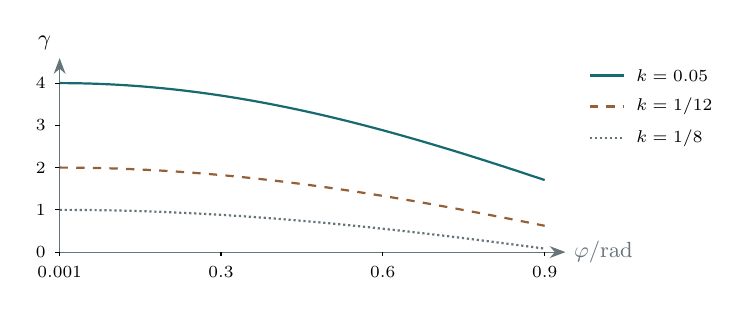
\begin{tikzpicture}[scale=.88,transform shape]
\draw[axis] (0,0.0)--(7.3,0.0) node[right] {$\varphi/\mathrm{rad}$};
\draw[axis] (0,0)--(0,2.8);
\node[above left] at (0,2.8) {$\gamma$};
\draw[thin] (0.000000,0.0)--(0.000000,-0.06);\node[below,font=\scriptsize] at (0.000000,-0.08) {$ 0.001 $};
\draw[thin] (2.328142,0.0)--(2.328142,-0.06);\node[below,font=\scriptsize] at (2.328142,-0.08) {$ 0.3 $};
\draw[thin] (4.664071,0.0)--(4.664071,-0.06);\node[below,font=\scriptsize] at (4.664071,-0.08) {$ 0.6 $};
\draw[thin] (7.000000,0.0)--(7.000000,-0.06);\node[below,font=\scriptsize] at (7.000000,-0.08) {$ 0.9 $};
\draw[thin] (0,0.000000)--(-.06,0.000000);\node[left,font=\scriptsize] at (-.08,0.000000) {$ 0 $};
\draw[thin] (0,0.609756)--(-.06,0.609756);\node[left,font=\scriptsize] at (-.08,0.609756) {$ 1 $};
\draw[thin] (0,1.219512)--(-.06,1.219512);\node[left,font=\scriptsize] at (-.08,1.219512) {$ 2 $};
\draw[thin] (0,1.829268)--(-.06,1.829268);\node[left,font=\scriptsize] at (-.08,1.829268) {$ 3 $};
\draw[thin] (0,2.439024)--(-.06,2.439024);\node[left,font=\scriptsize] at (-.08,2.439024) {$ 4 $};
\draw[thick,color=accent] plot coordinates {(0.0000000,2.4390224) (0.0291667,2.4389786) (0.0583333,2.4388778) (0.0875000,2.4387200) (0.1166667,2.4385052) (0.1458333,2.4382333) (0.1750000,2.4379044) (0.2041667,2.4375186) (0.2333333,2.4370757) (0.2625000,2.4365759) (0.2916667,2.4360191) (0.3208333,2.4354054) (0.3500000,2.4347347) (0.3791667,2.4340072) (0.4083333,2.4332228) (0.4375000,2.4323816) (0.4666667,2.4314835) (0.4958333,2.4305287) (0.5250000,2.4295171) (0.5541667,2.4284488) (0.5833333,2.4273238) (0.6125000,2.4261421) (0.6416667,2.4249039) (0.6708333,2.4236091) (0.7000000,2.4222578) (0.7291667,2.4208500) (0.7583333,2.4193858) (0.7875000,2.4178652) (0.8166667,2.4162883) (0.8458333,2.4146551) (0.8750000,2.4129657) (0.9041667,2.4112201) (0.9333333,2.4094184) (0.9625000,2.4075607) (0.9916667,2.4056470) (1.0208333,2.4036774) (1.0500000,2.4016520) (1.0791667,2.3995708) (1.1083333,2.3974338) (1.1375000,2.3952412) (1.1666667,2.3929931) (1.1958333,2.3906895) (1.2250000,2.3883304) (1.2541667,2.3859160) (1.2833333,2.3834464) (1.3125000,2.3809216) (1.3416667,2.3783417) (1.3708333,2.3757069) (1.4000000,2.3730171) (1.4291667,2.3702725) (1.4583333,2.3674732) (1.4875000,2.3646192) (1.5166667,2.3617107) (1.5458333,2.3587478) (1.5750000,2.3557305) (1.6041667,2.3526590) (1.6333333,2.3495334) (1.6625000,2.3463537) (1.6916667,2.3431201) (1.7208333,2.3398327) (1.7500000,2.3364916) (1.7791667,2.3330969) (1.8083333,2.3296487) (1.8375000,2.3261472) (1.8666667,2.3225924) (1.8958333,2.3189845) (1.9250000,2.3153236) (1.9541667,2.3116098) (1.9833333,2.3078432) (2.0125000,2.3040241) (2.0416667,2.3001524) (2.0708333,2.2962283) (2.1000000,2.2922520) (2.1291667,2.2882236) (2.1583333,2.2841432) (2.1875000,2.2800110) (2.2166667,2.2758271) (2.2458333,2.2715916) (2.2750000,2.2673047) (2.3041667,2.2629665) (2.3333333,2.2585772) (2.3625000,2.2541370) (2.3916667,2.2496458) (2.4208333,2.2451040) (2.4500000,2.2405117) (2.4791667,2.2358690) (2.5083333,2.2311761) (2.5375000,2.2264331) (2.5666667,2.2216402) (2.5958333,2.2167975) (2.6250000,2.2119053) (2.6541667,2.2069636) (2.6833333,2.2019727) (2.7125000,2.1969327) (2.7416667,2.1918438) (2.7708333,2.1867061) (2.8000000,2.1815198) (2.8291667,2.1762851) (2.8583333,2.1710022) (2.8875000,2.1656712) (2.9166667,2.1602924) (2.9458333,2.1548658) (2.9750000,2.1493918) (3.0041667,2.1438703) (3.0333333,2.1383018) (3.0625000,2.1326862) (3.0916667,2.1270239) (3.1208333,2.1213150) (3.1500000,2.1155597) (3.1791667,2.1097581) (3.2083333,2.1039106) (3.2375000,2.0980172) (3.2666667,2.0920782) (3.2958333,2.0860937) (3.3250000,2.0800640) (3.3541667,2.0739893) (3.3833333,2.0678698) (3.4125000,2.0617056) (3.4416667,2.0554970) (3.4708333,2.0492441) (3.5000000,2.0429473) (3.5291667,2.0366066) (3.5583333,2.0302224) (3.5875000,2.0237948) (3.6166667,2.0173240) (3.6458333,2.0108103) (3.6750000,2.0042538) (3.7041667,1.9976548) (3.7333333,1.9910134) (3.7625000,1.9843301) (3.7916667,1.9776048) (3.8208333,1.9708379) (3.8500000,1.9640296) (3.8791667,1.9571800) (3.9083333,1.9502896) (3.9375000,1.9433583) (3.9666667,1.9363866) (3.9958333,1.9293746) (4.0250000,1.9223225) (4.0541667,1.9152306) (4.0833333,1.9080992) (4.1125000,1.9009283) (4.1416667,1.8937184) (4.1708333,1.8864696) (4.2000000,1.8791822) (4.2291667,1.8718563) (4.2583333,1.8644923) (4.2875000,1.8570904) (4.3166667,1.8496508) (4.3458333,1.8421738) (4.3750000,1.8346596) (4.4041667,1.8271085) (4.4333333,1.8195207) (4.4625000,1.8118964) (4.4916667,1.8042360) (4.5208333,1.7965396) (4.5500000,1.7888075) (4.5791667,1.7810400) (4.6083333,1.7732373) (4.6375000,1.7653997) (4.6666667,1.7575275) (4.6958333,1.7496208) (4.7250000,1.7416799) (4.7541667,1.7337052) (4.7833333,1.7256969) (4.8125000,1.7176551) (4.8416667,1.7095803) (4.8708333,1.7014726) (4.9000000,1.6933324) (4.9291667,1.6851598) (4.9583333,1.6769552) (4.9875000,1.6687188) (5.0166667,1.6604509) (5.0458333,1.6521518) (5.0750000,1.6438216) (5.1041667,1.6354608) (5.1333333,1.6270695) (5.1625000,1.6186481) (5.1916667,1.6101968) (5.2208333,1.6017159) (5.2500000,1.5932056) (5.2791667,1.5846663) (5.3083333,1.5760982) (5.3375000,1.5675016) (5.3666667,1.5588768) (5.3958333,1.5502240) (5.4250000,1.5415435) (5.4541667,1.5328357) (5.4833333,1.5241007) (5.5125000,1.5153389) (5.5416667,1.5065506) (5.5708333,1.4977360) (5.6000000,1.4888954) (5.6291667,1.4800292) (5.6583333,1.4711375) (5.6875000,1.4622207) (5.7166667,1.4532791) (5.7458333,1.4443130) (5.7750000,1.4353226) (5.8041667,1.4263082) (5.8333333,1.4172701) (5.8625000,1.4082086) (5.8916667,1.3991241) (5.9208333,1.3900167) (5.9500000,1.3808868) (5.9791667,1.3717347) (6.0083333,1.3625607) (6.0375000,1.3533650) (6.0666667,1.3441480) (6.0958333,1.3349100) (6.1250000,1.3256511) (6.1541667,1.3163719) (6.1833333,1.3070724) (6.2125000,1.2977531) (6.2416667,1.2884142) (6.2708333,1.2790561) (6.3000000,1.2696789) (6.3291667,1.2602831) (6.3583333,1.2508689) (6.3875000,1.2414367) (6.4166667,1.2319866) (6.4458333,1.2225191) (6.4750000,1.2130343) (6.5041667,1.2035327) (6.5333333,1.1940145) (6.5625000,1.1844801) (6.5916667,1.1749296) (6.6208333,1.1653635) (6.6500000,1.1557820) (6.6791667,1.1461854) (6.7083333,1.1365741) (6.7375000,1.1269483) (6.7666667,1.1173083) (6.7958333,1.1076544) (6.8250000,1.0979870) (6.8541667,1.0883064) (6.8833333,1.0786127) (6.9125000,1.0689065) (6.9416667,1.0591879) (6.9708333,1.0494572) (7.0000000,1.0397148)};
\draw[thick,color=accent] (7.65,2.55)--(8.15,2.55);\node[right,font=\scriptsize] at (8.2,2.55) {$k=0.05$};
\draw[thick,dashed,color=warm] plot coordinates {(0.0000000,1.2195110) (0.0291667,1.2194847) (0.0583333,1.2194243) (0.0875000,1.2193296) (0.1166667,1.2192007) (0.1458333,1.2190375) (0.1750000,1.2188402) (0.2041667,1.2186087) (0.2333333,1.2183430) (0.2625000,1.2180431) (0.2916667,1.2177090) (0.3208333,1.2173408) (0.3500000,1.2169384) (0.3791667,1.2165019) (0.4083333,1.2160312) (0.4375000,1.2155265) (0.4666667,1.2149877) (0.4958333,1.2144148) (0.5250000,1.2138078) (0.5541667,1.2131668) (0.5833333,1.2124918) (0.6125000,1.2117828) (0.6416667,1.2110399) (0.6708333,1.2102630) (0.7000000,1.2094522) (0.7291667,1.2086076) (0.7583333,1.2077290) (0.7875000,1.2068167) (0.8166667,1.2058705) (0.8458333,1.2048906) (0.8750000,1.2038770) (0.9041667,1.2028296) (0.9333333,1.2017486) (0.9625000,1.2006340) (0.9916667,1.1994858) (1.0208333,1.1983040) (1.0500000,1.1970888) (1.0791667,1.1958400) (1.1083333,1.1945578) (1.1375000,1.1932423) (1.1666667,1.1918934) (1.1958333,1.1905112) (1.2250000,1.1890958) (1.2541667,1.1876472) (1.2833333,1.1861654) (1.3125000,1.1846505) (1.3416667,1.1831026) (1.3708333,1.1815217) (1.4000000,1.1799078) (1.4291667,1.1782611) (1.4583333,1.1765815) (1.4875000,1.1748691) (1.5166667,1.1731240) (1.5458333,1.1713462) (1.5750000,1.1695359) (1.6041667,1.1676930) (1.6333333,1.1658176) (1.6625000,1.1639098) (1.6916667,1.1619696) (1.7208333,1.1599972) (1.7500000,1.1579925) (1.7791667,1.1559557) (1.8083333,1.1538868) (1.8375000,1.1517859) (1.8666667,1.1496530) (1.8958333,1.1474883) (1.9250000,1.1452917) (1.9541667,1.1430634) (1.9833333,1.1408035) (2.0125000,1.1385120) (2.0416667,1.1361890) (2.0708333,1.1338346) (2.1000000,1.1314488) (2.1291667,1.1290317) (2.1583333,1.1265835) (2.1875000,1.1241042) (2.2166667,1.1215938) (2.2458333,1.1190525) (2.2750000,1.1164804) (2.3041667,1.1138775) (2.3333333,1.1112439) (2.3625000,1.1085797) (2.3916667,1.1058851) (2.4208333,1.1031600) (2.4500000,1.1004046) (2.4791667,1.0976190) (2.5083333,1.0948032) (2.5375000,1.0919574) (2.5666667,1.0890817) (2.5958333,1.0861761) (2.6250000,1.0832407) (2.6541667,1.0802757) (2.6833333,1.0772812) (2.7125000,1.0742572) (2.7416667,1.0712038) (2.7708333,1.0681212) (2.8000000,1.0650094) (2.8291667,1.0618686) (2.8583333,1.0586989) (2.8875000,1.0555003) (2.9166667,1.0522730) (2.9458333,1.0490171) (2.9750000,1.0457326) (3.0041667,1.0424198) (3.0333333,1.0390786) (3.0625000,1.0357093) (3.0916667,1.0323119) (3.1208333,1.0288866) (3.1500000,1.0254334) (3.1791667,1.0219524) (3.2083333,1.0184439) (3.2375000,1.0149079) (3.2666667,1.0113445) (3.2958333,1.0077538) (3.3250000,1.0041360) (3.3541667,1.0004911) (3.3833333,0.9968194) (3.4125000,0.9931209) (3.4416667,0.9893957) (3.4708333,0.9856440) (3.5000000,0.9818659) (3.5291667,0.9780616) (3.5583333,0.9742310) (3.5875000,0.9703744) (3.6166667,0.9664920) (3.6458333,0.9625837) (3.6750000,0.9586498) (3.7041667,0.9546904) (3.7333333,0.9507056) (3.7625000,0.9466956) (3.7916667,0.9426604) (3.8208333,0.9386003) (3.8500000,0.9345153) (3.8791667,0.9304056) (3.9083333,0.9262713) (3.9375000,0.9221126) (3.9666667,0.9179295) (3.9958333,0.9137223) (4.0250000,0.9094911) (4.0541667,0.9052359) (4.0833333,0.9009571) (4.1125000,0.8966546) (4.1416667,0.8923286) (4.1708333,0.8879793) (4.2000000,0.8836069) (4.2291667,0.8792114) (4.2583333,0.8747930) (4.2875000,0.8703518) (4.3166667,0.8658881) (4.3458333,0.8614018) (4.3750000,0.8568933) (4.4041667,0.8523626) (4.4333333,0.8478100) (4.4625000,0.8432354) (4.4916667,0.8386391) (4.5208333,0.8340213) (4.5500000,0.8293821) (4.5791667,0.8247216) (4.6083333,0.8200400) (4.6375000,0.8153374) (4.6666667,0.8106140) (4.6958333,0.8058700) (4.7250000,0.8011055) (4.7541667,0.7963207) (4.7833333,0.7915157) (4.8125000,0.7866907) (4.8416667,0.7818458) (4.8708333,0.7769811) (4.9000000,0.7720970) (4.9291667,0.7671935) (4.9583333,0.7622707) (4.9875000,0.7573289) (5.0166667,0.7523681) (5.0458333,0.7473886) (5.0750000,0.7423905) (5.1041667,0.7373740) (5.1333333,0.7323393) (5.1625000,0.7272864) (5.1916667,0.7222156) (5.2208333,0.7171271) (5.2500000,0.7120209) (5.2791667,0.7068973) (5.3083333,0.7017565) (5.3375000,0.6965985) (5.3666667,0.6914236) (5.3958333,0.6862319) (5.4250000,0.6810237) (5.4541667,0.6757990) (5.4833333,0.6705580) (5.5125000,0.6653009) (5.5416667,0.6600279) (5.5708333,0.6547392) (5.6000000,0.6494348) (5.6291667,0.6441151) (5.6583333,0.6387801) (5.6875000,0.6334300) (5.7166667,0.6280650) (5.7458333,0.6226853) (5.7750000,0.6172911) (5.8041667,0.6118825) (5.8333333,0.6064596) (5.8625000,0.6010227) (5.8916667,0.5955720) (5.9208333,0.5901076) (5.9500000,0.5846297) (5.9791667,0.5791384) (6.0083333,0.5736340) (6.0375000,0.5681166) (6.0666667,0.5625864) (6.0958333,0.5570435) (6.1250000,0.5514882) (6.1541667,0.5459207) (6.1833333,0.5403410) (6.2125000,0.5347494) (6.2416667,0.5291461) (6.2708333,0.5235312) (6.3000000,0.5179049) (6.3291667,0.5122674) (6.3583333,0.5066189) (6.3875000,0.5009596) (6.4166667,0.4952895) (6.4458333,0.4896090) (6.4750000,0.4839182) (6.5041667,0.4782172) (6.5333333,0.4725063) (6.5625000,0.4667856) (6.5916667,0.4610553) (6.6208333,0.4553157) (6.6500000,0.4495668) (6.6791667,0.4438088) (6.7083333,0.4380420) (6.7375000,0.4322665) (6.7666667,0.4264825) (6.7958333,0.4206902) (6.8250000,0.4148898) (6.8541667,0.4090814) (6.8833333,0.4032652) (6.9125000,0.3974414) (6.9416667,0.3916103) (6.9708333,0.3857719) (7.0000000,0.3799265)};
\draw[thick,dashed,color=warm] (7.65,2.0999999999999996)--(8.15,2.0999999999999996);\node[right,font=\scriptsize] at (8.2,2.0999999999999996) {$k=1/12$};
\draw[densely dotted,thick,color=muted] plot coordinates {(0.0000000,0.6097553) (0.0291667,0.6097378) (0.0583333,0.6096975) (0.0875000,0.6096343) (0.1166667,0.6095484) (0.1458333,0.6094397) (0.1750000,0.6093081) (0.2041667,0.6091538) (0.2333333,0.6089766) (0.2625000,0.6087767) (0.2916667,0.6085540) (0.3208333,0.6083085) (0.3500000,0.6080402) (0.3791667,0.6077492) (0.4083333,0.6074355) (0.4375000,0.6070990) (0.4666667,0.6067397) (0.4958333,0.6063578) (0.5250000,0.6059532) (0.5541667,0.6055258) (0.5833333,0.6050759) (0.6125000,0.6046032) (0.6416667,0.6041079) (0.6708333,0.6035900) (0.7000000,0.6030495) (0.7291667,0.6024863) (0.7583333,0.6019007) (0.7875000,0.6012924) (0.8166667,0.6006617) (0.8458333,0.6000084) (0.8750000,0.5993326) (0.9041667,0.5986344) (0.9333333,0.5979137) (0.9625000,0.5971706) (0.9916667,0.5964052) (1.0208333,0.5956173) (1.0500000,0.5948071) (1.0791667,0.5939746) (1.1083333,0.5931199) (1.1375000,0.5922428) (1.1666667,0.5913436) (1.1958333,0.5904221) (1.2250000,0.5894785) (1.2541667,0.5885128) (1.2833333,0.5875249) (1.3125000,0.5865150) (1.3416667,0.5854830) (1.3708333,0.5844291) (1.4000000,0.5833532) (1.4291667,0.5822553) (1.4583333,0.5811356) (1.4875000,0.5799940) (1.5166667,0.5788306) (1.5458333,0.5776455) (1.5750000,0.5764385) (1.6041667,0.5752099) (1.6333333,0.5739597) (1.6625000,0.5726878) (1.6916667,0.5713944) (1.7208333,0.5700794) (1.7500000,0.5687430) (1.7791667,0.5673851) (1.8083333,0.5660058) (1.8375000,0.5646052) (1.8666667,0.5631833) (1.8958333,0.5617401) (1.9250000,0.5602758) (1.9541667,0.5587903) (1.9833333,0.5572836) (2.0125000,0.5557560) (2.0416667,0.5542073) (2.0708333,0.5526377) (2.1000000,0.5510471) (2.1291667,0.5494358) (2.1583333,0.5478036) (2.1875000,0.5461507) (2.2166667,0.5444772) (2.2458333,0.5427830) (2.2750000,0.5410682) (2.3041667,0.5393330) (2.3333333,0.5375772) (2.3625000,0.5358011) (2.3916667,0.5340047) (2.4208333,0.5321880) (2.4500000,0.5303510) (2.4791667,0.5284939) (2.5083333,0.5266168) (2.5375000,0.5247196) (2.5666667,0.5228024) (2.5958333,0.5208654) (2.6250000,0.5189085) (2.6541667,0.5169318) (2.6833333,0.5149354) (2.7125000,0.5129194) (2.7416667,0.5108838) (2.7708333,0.5088288) (2.8000000,0.5067543) (2.8291667,0.5046604) (2.8583333,0.5025472) (2.8875000,0.5004148) (2.9166667,0.4982633) (2.9458333,0.4960927) (2.9750000,0.4939030) (3.0041667,0.4916945) (3.0333333,0.4894670) (3.0625000,0.4872208) (3.0916667,0.4849559) (3.1208333,0.4826723) (3.1500000,0.4803702) (3.1791667,0.4780496) (3.2083333,0.4757106) (3.2375000,0.4733532) (3.2666667,0.4709776) (3.2958333,0.4685838) (3.3250000,0.4661720) (3.3541667,0.4637421) (3.3833333,0.4612942) (3.4125000,0.4588286) (3.4416667,0.4563451) (3.4708333,0.4538440) (3.5000000,0.4513253) (3.5291667,0.4487890) (3.5583333,0.4462353) (3.5875000,0.4436643) (3.6166667,0.4410759) (3.6458333,0.4384704) (3.6750000,0.4358478) (3.7041667,0.4332082) (3.7333333,0.4305517) (3.7625000,0.4278784) (3.7916667,0.4251883) (3.8208333,0.4224815) (3.8500000,0.4197582) (3.8791667,0.4170184) (3.9083333,0.4142622) (3.9375000,0.4114897) (3.9666667,0.4087010) (3.9958333,0.4058962) (4.0250000,0.4030753) (4.0541667,0.4002386) (4.0833333,0.3973860) (4.1125000,0.3945177) (4.1416667,0.3916337) (4.1708333,0.3887342) (4.2000000,0.3858192) (4.2291667,0.3828889) (4.2583333,0.3799433) (4.2875000,0.3769825) (4.3166667,0.3740067) (4.3458333,0.3710159) (4.3750000,0.3680102) (4.4041667,0.3649897) (4.4333333,0.3619546) (4.4625000,0.3589049) (4.4916667,0.3558407) (4.5208333,0.3527622) (4.5500000,0.3496693) (4.5791667,0.3465623) (4.6083333,0.3434413) (4.6375000,0.3403062) (4.6666667,0.3371573) (4.6958333,0.3339947) (4.7250000,0.3308183) (4.7541667,0.3276284) (4.7833333,0.3244251) (4.8125000,0.3212084) (4.8416667,0.3179785) (4.8708333,0.3147354) (4.9000000,0.3114793) (4.9291667,0.3082103) (4.9583333,0.3049284) (4.9875000,0.3016339) (5.0166667,0.2983267) (5.0458333,0.2950070) (5.0750000,0.2916750) (5.1041667,0.2883307) (5.1333333,0.2849742) (5.1625000,0.2816056) (5.1916667,0.2782251) (5.2208333,0.2748327) (5.2500000,0.2714286) (5.2791667,0.2680129) (5.3083333,0.2645856) (5.3375000,0.2611470) (5.3666667,0.2576970) (5.3958333,0.2542359) (5.4250000,0.2507637) (5.4541667,0.2472806) (5.4833333,0.2437866) (5.5125000,0.2402819) (5.5416667,0.2367666) (5.5708333,0.2332407) (5.6000000,0.2297045) (5.6291667,0.2261580) (5.6583333,0.2226014) (5.6875000,0.2190346) (5.7166667,0.2154580) (5.7458333,0.2118715) (5.7750000,0.2082754) (5.8041667,0.2046696) (5.8333333,0.2010544) (5.8625000,0.1974298) (5.8916667,0.1937960) (5.9208333,0.1901530) (5.9500000,0.1865011) (5.9791667,0.1828402) (6.0083333,0.1791706) (6.0375000,0.1754924) (6.0666667,0.1718056) (6.0958333,0.1681103) (6.1250000,0.1644068) (6.1541667,0.1606951) (6.1833333,0.1569753) (6.2125000,0.1532476) (6.2416667,0.1495120) (6.2708333,0.1457688) (6.3000000,0.1420179) (6.3291667,0.1382596) (6.3583333,0.1344939) (6.3875000,0.1307210) (6.4166667,0.1269410) (6.4458333,0.1231540) (6.4750000,0.1193601) (6.5041667,0.1155594) (6.5333333,0.1117522) (6.5625000,0.1079384) (6.5916667,0.1041182) (6.6208333,0.1002917) (6.6500000,0.0964591) (6.6791667,0.0926205) (6.7083333,0.0887760) (6.7375000,0.0849256) (6.7666667,0.0810697) (6.7958333,0.0772081) (6.8250000,0.0733412) (6.8541667,0.0694689) (6.8833333,0.0655914) (6.9125000,0.0617089) (6.9416667,0.0578215) (6.9708333,0.0539292) (7.0000000,0.0500323)};
\draw[densely dotted,thick,color=muted] (7.65,1.65)--(8.15,1.65);\node[right,font=\scriptsize] at (8.2,1.65) {$k=1/8$};
\end{tikzpicture}
\figcaption{变图力试1.4V4\quad 三种杆惯量系数对应的质量角度关系}
\end{minipage}\end{center}
\item \textbf{弹簧能量的分配。}求球离杆瞬间，球平动、杆平动、杆自转的总动能，并由给定释放能量$E_s$反求$v$。

动量与角动量给$V_C=v/\gamma$、$\Omega=6v\sin\varphi/(\gamma l)$，因此
\[
 E_s=\frac12mv^2+\frac12MV_C^2+\frac12I_C\Omega^2
 =\frac12mv^2\left[1+\frac{1+3\sin^2\varphi}{\gamma}\right],
\quad
 v=\sqrt{\frac{2E_s/m}{1+(1+3\sin^2\varphi)/\gamma}}.
\]
变图力试1.4V5沿相遇配对曲线画能量倍率，质量比很小时杆的平移和转动占更大份额。释放能量确定速率，质量与角度仍由相遇几何关系配对。
\begin{center}\begin{minipage}{.98\linewidth}\centering
\begin{tikzpicture}[scale=.88,transform shape]
\draw[axis] (0,0.0)--(7.3,0.0) node[right] {$\gamma$};
\draw[axis] (0,0)--(0,2.8);
\node[above left] at (0,2.8) {$2E_s/(mv^2)$};
\draw[thin] (0.000000,0.0)--(0.000000,-0.06);\node[below,font=\scriptsize] at (0.000000,-0.08) {$ 0.1 $};
\draw[thin] (1.555556,0.0)--(1.555556,-0.06);\node[below,font=\scriptsize] at (1.555556,-0.08) {$ 0.5 $};
\draw[thin] (3.500000,0.0)--(3.500000,-0.06);\node[below,font=\scriptsize] at (3.500000,-0.08) {$ 1 $};
\draw[thin] (5.444444,0.0)--(5.444444,-0.06);\node[below,font=\scriptsize] at (5.444444,-0.08) {$ 1.5 $};
\draw[thin] (7.000000,0.0)--(7.000000,-0.06);\node[below,font=\scriptsize] at (7.000000,-0.08) {$ 1.9 $};
\draw[thin] (0,0.000000)--(-.06,0.000000);\node[left,font=\scriptsize] at (-.08,0.000000) {$ 0 $};
\draw[thin] (0,0.347222)--(-.06,0.347222);\node[left,font=\scriptsize] at (-.08,0.347222) {$ 5 $};
\draw[thin] (0,0.694444)--(-.06,0.694444);\node[left,font=\scriptsize] at (-.08,0.694444) {$ 10 $};
\draw[thin] (0,1.388889)--(-.06,1.388889);\node[left,font=\scriptsize] at (-.08,1.388889) {$ 20 $};
\draw[thin] (0,2.083333)--(-.06,2.083333);\node[left,font=\scriptsize] at (-.08,2.083333) {$ 30 $};
\draw[thick,color=accent] plot coordinates {(0.0000000,2.4201884) (0.0291667,2.2516730) (0.0583333,2.1051218) (0.0875000,1.9765006) (0.1166667,1.8627063) (0.1458333,1.7613127) (0.1750000,1.6703956) (0.2041667,1.5884094) (0.2333333,1.5140982) (0.2625000,1.4464311) (0.2916667,1.3845539) (0.3208333,1.3277528) (0.3500000,1.2754268) (0.3791667,1.2270661) (0.4083333,1.1822355) (0.4375000,1.1405612) (0.4666667,1.1017206) (0.4958333,1.0654333) (0.5250000,1.0314550) (0.5541667,0.9995715) (0.5833333,0.9695942) (0.6125000,0.9413567) (0.6416667,0.9147111) (0.6708333,0.8895262) (0.7000000,0.8656846) (0.7291667,0.8430811) (0.7583333,0.8216215) (0.7875000,0.8012205) (0.8166667,0.7818014) (0.8458333,0.7632947) (0.8750000,0.7456371) (0.9041667,0.7287713) (0.9333333,0.7126449) (0.9625000,0.6972101) (0.9916667,0.6824229) (1.0208333,0.6682433) (1.0500000,0.6546343) (1.0791667,0.6415619) (1.1083333,0.6289948) (1.1375000,0.6169040) (1.1666667,0.6052627) (1.1958333,0.5940462) (1.2250000,0.5832315) (1.2541667,0.5727971) (1.2833333,0.5627232) (1.3125000,0.5529912) (1.3416667,0.5435839) (1.3708333,0.5344851) (1.4000000,0.5256798) (1.4291667,0.5171538) (1.4583333,0.5088940) (1.4875000,0.5008879) (1.5166667,0.4931239) (1.5458333,0.4855911) (1.5750000,0.4782791) (1.6041667,0.4711783) (1.6333333,0.4642796) (1.6625000,0.4575744) (1.6916667,0.4510544) (1.7208333,0.4447122) (1.7500000,0.4385403) (1.7791667,0.4325319) (1.8083333,0.4266806) (1.8375000,0.4209801) (1.8666667,0.4154247) (1.8958333,0.4100087) (1.9250000,0.4047270) (1.9541667,0.3995745) (1.9833333,0.3945464) (2.0125000,0.3896382) (2.0416667,0.3848457) (2.0708333,0.3801647) (2.1000000,0.3755913) (2.1291667,0.3711217) (2.1583333,0.3667525) (2.1875000,0.3624801) (2.2166667,0.3583015) (2.2458333,0.3542134) (2.2750000,0.3502129) (2.3041667,0.3462971) (2.3333333,0.3424634) (2.3625000,0.3387091) (2.3916667,0.3350318) (2.4208333,0.3314290) (2.4500000,0.3278985) (2.4791667,0.3244380) (2.5083333,0.3210456) (2.5375000,0.3177190) (2.5666667,0.3144564) (2.5958333,0.3112559) (2.6250000,0.3081158) (2.6541667,0.3050342) (2.6833333,0.3020096) (2.7125000,0.2990403) (2.7416667,0.2961247) (2.7708333,0.2932615) (2.8000000,0.2904491) (2.8291667,0.2876863) (2.8583333,0.2849716) (2.8875000,0.2823038) (2.9166667,0.2796816) (2.9458333,0.2771039) (2.9750000,0.2745694) (3.0041667,0.2720772) (3.0333333,0.2696261) (3.0625000,0.2672151) (3.0916667,0.2648432) (3.1208333,0.2625093) (3.1500000,0.2602126) (3.1791667,0.2579522) (3.2083333,0.2557272) (3.2375000,0.2535367) (3.2666667,0.2513799) (3.2958333,0.2492561) (3.3250000,0.2471644) (3.3541667,0.2451041) (3.3833333,0.2430744) (3.4125000,0.2410747) (3.4416667,0.2391044) (3.4708333,0.2371626) (3.5000000,0.2352488) (3.5291667,0.2333625) (3.5583333,0.2315028) (3.5875000,0.2296694) (3.6166667,0.2278615) (3.6458333,0.2260788) (3.6750000,0.2243205) (3.7041667,0.2225863) (3.7333333,0.2208755) (3.7625000,0.2191878) (3.7916667,0.2175226) (3.8208333,0.2158794) (3.8500000,0.2142579) (3.8791667,0.2126575) (3.9083333,0.2110779) (3.9375000,0.2095186) (3.9666667,0.2079792) (3.9958333,0.2064593) (4.0250000,0.2049586) (4.0541667,0.2034766) (4.0833333,0.2020131) (4.1125000,0.2005676) (4.1416667,0.1991398) (4.1708333,0.1977294) (4.2000000,0.1963360) (4.2291667,0.1949593) (4.2583333,0.1935990) (4.2875000,0.1922549) (4.3166667,0.1909265) (4.3458333,0.1896137) (4.3750000,0.1883160) (4.4041667,0.1870334) (4.4333333,0.1857654) (4.4625000,0.1845119) (4.4916667,0.1832725) (4.5208333,0.1820470) (4.5500000,0.1808353) (4.5791667,0.1796369) (4.6083333,0.1784518) (4.6375000,0.1772796) (4.6666667,0.1761202) (4.6958333,0.1749733) (4.7250000,0.1738388) (4.7541667,0.1727164) (4.7833333,0.1716059) (4.8125000,0.1705071) (4.8416667,0.1694198) (4.8708333,0.1683438) (4.9000000,0.1672790) (4.9291667,0.1662252) (4.9583333,0.1651822) (4.9875000,0.1641497) (5.0166667,0.1631278) (5.0458333,0.1621161) (5.0750000,0.1611145) (5.1041667,0.1601228) (5.1333333,0.1591410) (5.1625000,0.1581688) (5.1916667,0.1572062) (5.2208333,0.1562528) (5.2500000,0.1553087) (5.2791667,0.1543737) (5.3083333,0.1534475) (5.3375000,0.1525302) (5.3666667,0.1516216) (5.3958333,0.1507215) (5.4250000,0.1498297) (5.4541667,0.1489463) (5.4833333,0.1480711) (5.5125000,0.1472038) (5.5416667,0.1463446) (5.5708333,0.1454931) (5.6000000,0.1446493) (5.6291667,0.1438131) (5.6583333,0.1429844) (5.6875000,0.1421631) (5.7166667,0.1413490) (5.7458333,0.1405421) (5.7750000,0.1397423) (5.8041667,0.1389494) (5.8333333,0.1381634) (5.8625000,0.1373842) (5.8916667,0.1366117) (5.9208333,0.1358458) (5.9500000,0.1350864) (5.9791667,0.1343334) (6.0083333,0.1335867) (6.0375000,0.1328463) (6.0666667,0.1321120) (6.0958333,0.1313838) (6.1250000,0.1306617) (6.1541667,0.1299454) (6.1833333,0.1292350) (6.2125000,0.1285303) (6.2416667,0.1278314) (6.2708333,0.1271380) (6.3000000,0.1264502) (6.3291667,0.1257679) (6.3583333,0.1250910) (6.3875000,0.1244195) (6.4166667,0.1237532) (6.4458333,0.1230921) (6.4750000,0.1224361) (6.5041667,0.1217852) (6.5333333,0.1211394) (6.5625000,0.1204985) (6.5916667,0.1198624) (6.6208333,0.1192312) (6.6500000,0.1186048) (6.6791667,0.1179831) (6.7083333,0.1173661) (6.7375000,0.1167536) (6.7666667,0.1161457) (6.7958333,0.1155423) (6.8250000,0.1149433) (6.8541667,0.1143487) (6.8833333,0.1137584) (6.9125000,0.1131724) (6.9416667,0.1125907) (6.9708333,0.1120131) (7.0000000,0.1114397)};
\end{tikzpicture}
\figcaption{变图力试1.4V5\quad 配对相遇状态的球杆总动能倍率}
\end{minipage}\end{center}
\item \textbf{地面相遇坐标。}沿用变式1，写球与A端的地面轨迹并求相遇点。

设$t_c=\cos\varphi/2$。球从$(1/2,0)$出发，$\boldsymbol r_b=(1/2,0)+t(-\cos\varphi,\sin\varphi)$。杆质心$\boldsymbol r_C=t(\cos\varphi,-\sin\varphi)$，A端为
\[
 \boldsymbol r_A=\boldsymbol r_C+
 \tfrac12(-\cos\Omega t,\sin\Omega t).
\]
在$t=t_c$，$\Omega t_c=2\varphi$，两坐标相等，给$\boldsymbol r_*=(\tfrac12\sin^2\varphi,\tfrac12\sin\varphi\cos\varphi)\simeq(0.2313,0.2493)$。变图力试1.4V6画球直线和A端复合曲线在该点汇合，质心同时沿反向直线运动。
\begin{center}\begin{minipage}{.98\linewidth}\centering
\begin{tikzpicture}[scale=4]
\draw[axis] (-.6,0)--(.7,0) node[right] {$x/l$};\draw[axis] (0,-.8)--(0,.45) node[above] {$y/l$};
\draw[thick,color=accent] plot coordinates {(0.5000000,0.0000000) (0.4988803,0.0010387) (0.4977605,0.0020775) (0.4966408,0.0031162) (0.4955211,0.0041549) (0.4944013,0.0051937) (0.4932816,0.0062324) (0.4921619,0.0072712) (0.4910421,0.0083099) (0.4899224,0.0093486) (0.4888027,0.0103874) (0.4876829,0.0114261) (0.4865632,0.0124648) (0.4854435,0.0135036) (0.4843237,0.0145423) (0.4832040,0.0155811) (0.4820843,0.0166198) (0.4809645,0.0176585) (0.4798448,0.0186973) (0.4787251,0.0197360) (0.4776053,0.0207747) (0.4764856,0.0218135) (0.4753659,0.0228522) (0.4742461,0.0238910) (0.4731264,0.0249297) (0.4720067,0.0259684) (0.4708869,0.0270072) (0.4697672,0.0280459) (0.4686475,0.0290846) (0.4675277,0.0301234) (0.4664080,0.0311621) (0.4652883,0.0322009) (0.4641685,0.0332396) (0.4630488,0.0342783) (0.4619291,0.0353171) (0.4608093,0.0363558) (0.4596896,0.0373945) (0.4585699,0.0384333) (0.4574501,0.0394720) (0.4563304,0.0405108) (0.4552106,0.0415495) (0.4540909,0.0425882) (0.4529712,0.0436270) (0.4518514,0.0446657) (0.4507317,0.0457044) (0.4496120,0.0467432) (0.4484922,0.0477819) (0.4473725,0.0488206) (0.4462528,0.0498594) (0.4451330,0.0508981) (0.4440133,0.0519369) (0.4428936,0.0529756) (0.4417738,0.0540143) (0.4406541,0.0550531) (0.4395344,0.0560918) (0.4384146,0.0571305) (0.4372949,0.0581693) (0.4361752,0.0592080) (0.4350554,0.0602468) (0.4339357,0.0612855) (0.4328160,0.0623242) (0.4316962,0.0633630) (0.4305765,0.0644017) (0.4294568,0.0654404) (0.4283370,0.0664792) (0.4272173,0.0675179) (0.4260976,0.0685567) (0.4249778,0.0695954) (0.4238581,0.0706341) (0.4227384,0.0716729) (0.4216186,0.0727116) (0.4204989,0.0737503) (0.4193792,0.0747891) (0.4182594,0.0758278) (0.4171397,0.0768666) (0.4160200,0.0779053) (0.4149002,0.0789440) (0.4137805,0.0799828) (0.4126608,0.0810215) (0.4115410,0.0820602) (0.4104213,0.0830990) (0.4093016,0.0841377) (0.4081818,0.0851765) (0.4070621,0.0862152) (0.4059424,0.0872539) (0.4048226,0.0882927) (0.4037029,0.0893314) (0.4025832,0.0903701) (0.4014634,0.0914089) (0.4003437,0.0924476) (0.3992240,0.0934863) (0.3981042,0.0945251) (0.3969845,0.0955638) (0.3958648,0.0966026) (0.3947450,0.0976413) (0.3936253,0.0986800) (0.3925056,0.0997188) (0.3913858,0.1007575) (0.3902661,0.1017962) (0.3891464,0.1028350) (0.3880266,0.1038737) (0.3869069,0.1049125) (0.3857872,0.1059512) (0.3846674,0.1069899) (0.3835477,0.1080287) (0.3824280,0.1090674) (0.3813082,0.1101061) (0.3801885,0.1111449) (0.3790688,0.1121836) (0.3779490,0.1132224) (0.3768293,0.1142611) (0.3757096,0.1152998) (0.3745898,0.1163386) (0.3734701,0.1173773) (0.3723503,0.1184160) (0.3712306,0.1194548) (0.3701109,0.1204935) (0.3689911,0.1215323) (0.3678714,0.1225710) (0.3667517,0.1236097) (0.3656319,0.1246485) (0.3645122,0.1256872) (0.3633925,0.1267259) (0.3622727,0.1277647) (0.3611530,0.1288034) (0.3600333,0.1298422) (0.3589135,0.1308809) (0.3577938,0.1319196) (0.3566741,0.1329584) (0.3555543,0.1339971) (0.3544346,0.1350358) (0.3533149,0.1360746) (0.3521951,0.1371133) (0.3510754,0.1381520) (0.3499557,0.1391908) (0.3488359,0.1402295) (0.3477162,0.1412683) (0.3465965,0.1423070) (0.3454767,0.1433457) (0.3443570,0.1443845) (0.3432373,0.1454232) (0.3421175,0.1464619) (0.3409978,0.1475007) (0.3398781,0.1485394) (0.3387583,0.1495782) (0.3376386,0.1506169) (0.3365189,0.1516556) (0.3353991,0.1526944) (0.3342794,0.1537331) (0.3331597,0.1547718) (0.3320399,0.1558106) (0.3309202,0.1568493) (0.3298005,0.1578881) (0.3286807,0.1589268) (0.3275610,0.1599655) (0.3264413,0.1610043) (0.3253215,0.1620430) (0.3242018,0.1630817) (0.3230821,0.1641205) (0.3219623,0.1651592) (0.3208426,0.1661980) (0.3197229,0.1672367) (0.3186031,0.1682754) (0.3174834,0.1693142) (0.3163637,0.1703529) (0.3152439,0.1713916) (0.3141242,0.1724304) (0.3130045,0.1734691) (0.3118847,0.1745078) (0.3107650,0.1755466) (0.3096453,0.1765853) (0.3085255,0.1776241) (0.3074058,0.1786628) (0.3062861,0.1797015) (0.3051663,0.1807403) (0.3040466,0.1817790) (0.3029269,0.1828177) (0.3018071,0.1838565) (0.3006874,0.1848952) (0.2995677,0.1859340) (0.2984479,0.1869727) (0.2973282,0.1880114) (0.2962085,0.1890502) (0.2950887,0.1900889) (0.2939690,0.1911276) (0.2928493,0.1921664) (0.2917295,0.1932051) (0.2906098,0.1942439) (0.2894901,0.1952826) (0.2883703,0.1963213) (0.2872506,0.1973601) (0.2861308,0.1983988) (0.2850111,0.1994375) (0.2838914,0.2004763) (0.2827716,0.2015150) (0.2816519,0.2025538) (0.2805322,0.2035925) (0.2794124,0.2046312) (0.2782927,0.2056700) (0.2771730,0.2067087) (0.2760532,0.2077474) (0.2749335,0.2087862) (0.2738138,0.2098249) (0.2726940,0.2108637) (0.2715743,0.2119024) (0.2704546,0.2129411) (0.2693348,0.2139799) (0.2682151,0.2150186) (0.2670954,0.2160573) (0.2659756,0.2170961) (0.2648559,0.2181348) (0.2637362,0.2191735) (0.2626164,0.2202123) (0.2614967,0.2212510) (0.2603770,0.2222898) (0.2592572,0.2233285) (0.2581375,0.2243672) (0.2570178,0.2254060) (0.2558980,0.2264447) (0.2547783,0.2274834) (0.2536586,0.2285222) (0.2525388,0.2295609) (0.2514191,0.2305997) (0.2502994,0.2316384) (0.2491796,0.2326771) (0.2480599,0.2337159) (0.2469402,0.2347546) (0.2458204,0.2357933) (0.2447007,0.2368321) (0.2435810,0.2378708) (0.2424612,0.2389096) (0.2413415,0.2399483) (0.2402218,0.2409870) (0.2391020,0.2420258) (0.2379823,0.2430645) (0.2368626,0.2441032) (0.2357428,0.2451420) (0.2346231,0.2461807) (0.2335034,0.2472195) (0.2323836,0.2482582) (0.2312639,0.2492969)};
\draw[thick,dashed,color=warm] plot coordinates {(-0.5000000,0.0000000) (-0.4988706,0.0020775) (-0.4977217,0.0041548) (-0.4965534,0.0062319) (-0.4953657,0.0083086) (-0.4941586,0.0103849) (-0.4929321,0.0124605) (-0.4916861,0.0145354) (-0.4904208,0.0166095) (-0.4891360,0.0186826) (-0.4878319,0.0207546) (-0.4865084,0.0228254) (-0.4851655,0.0248948) (-0.4838032,0.0269629) (-0.4824216,0.0290293) (-0.4810207,0.0310941) (-0.4796004,0.0331570) (-0.4781607,0.0352180) (-0.4767018,0.0372770) (-0.4752236,0.0393337) (-0.4737260,0.0413882) (-0.4722092,0.0434403) (-0.4706732,0.0454898) (-0.4691179,0.0475367) (-0.4675434,0.0495808) (-0.4659497,0.0516220) (-0.4643368,0.0536602) (-0.4627047,0.0556953) (-0.4610535,0.0577271) (-0.4593832,0.0597555) (-0.4576937,0.0617805) (-0.4559852,0.0638018) (-0.4542576,0.0658194) (-0.4525110,0.0678332) (-0.4507453,0.0698430) (-0.4489607,0.0718487) (-0.4471571,0.0738502) (-0.4453346,0.0758474) (-0.4434932,0.0778401) (-0.4416329,0.0798283) (-0.4397537,0.0818119) (-0.4378557,0.0837906) (-0.4359390,0.0857644) (-0.4340034,0.0877332) (-0.4320492,0.0896968) (-0.4300762,0.0916552) (-0.4280846,0.0936082) (-0.4260744,0.0955558) (-0.4240455,0.0974977) (-0.4219981,0.0994339) (-0.4199322,0.1013642) (-0.4178478,0.1032886) (-0.4157449,0.1052069) (-0.4136237,0.1071191) (-0.4114840,0.1090249) (-0.4093261,0.1109243) (-0.4071498,0.1128172) (-0.4049553,0.1147035) (-0.4027426,0.1165830) (-0.4005117,0.1184556) (-0.3982627,0.1203213) (-0.3959956,0.1221798) (-0.3937104,0.1240312) (-0.3914073,0.1258752) (-0.3890863,0.1277118) (-0.3867473,0.1295409) (-0.3843905,0.1313623) (-0.3820159,0.1331759) (-0.3796236,0.1349817) (-0.3772135,0.1367794) (-0.3747858,0.1385691) (-0.3723405,0.1403506) (-0.3698776,0.1421237) (-0.3673972,0.1438885) (-0.3648994,0.1456447) (-0.3623842,0.1473922) (-0.3598517,0.1491310) (-0.3573018,0.1508610) (-0.3547348,0.1525819) (-0.3521506,0.1542938) (-0.3495492,0.1559966) (-0.3469308,0.1576900) (-0.3442954,0.1593740) (-0.3416431,0.1610486) (-0.3389739,0.1627135) (-0.3362878,0.1643687) (-0.3335850,0.1660141) (-0.3308655,0.1676496) (-0.3281294,0.1692751) (-0.3253767,0.1708904) (-0.3226075,0.1724956) (-0.3198218,0.1740904) (-0.3170198,0.1756747) (-0.3142014,0.1772485) (-0.3113668,0.1788117) (-0.3085161,0.1803641) (-0.3056492,0.1819057) (-0.3027662,0.1834364) (-0.2998673,0.1849560) (-0.2969524,0.1864645) (-0.2940218,0.1879618) (-0.2910753,0.1894477) (-0.2881132,0.1909221) (-0.2851354,0.1923851) (-0.2821421,0.1938364) (-0.2791332,0.1952760) (-0.2761090,0.1967038) (-0.2730695,0.1981196) (-0.2700146,0.1995235) (-0.2669446,0.2009152) (-0.2638595,0.2022947) (-0.2607594,0.2036620) (-0.2576443,0.2050168) (-0.2545143,0.2063592) (-0.2513695,0.2076890) (-0.2482100,0.2090061) (-0.2450359,0.2103105) (-0.2418471,0.2116020) (-0.2386439,0.2128805) (-0.2354263,0.2141461) (-0.2321944,0.2153985) (-0.2289483,0.2166377) (-0.2256880,0.2178636) (-0.2224136,0.2190762) (-0.2191252,0.2202752) (-0.2158229,0.2214607) (-0.2125068,0.2226326) (-0.2091770,0.2237907) (-0.2058335,0.2249350) (-0.2024765,0.2260654) (-0.1991060,0.2271819) (-0.1957220,0.2282842) (-0.1923248,0.2293724) (-0.1889144,0.2304464) (-0.1854909,0.2315060) (-0.1820543,0.2325513) (-0.1786048,0.2335820) (-0.1751424,0.2345983) (-0.1716673,0.2355998) (-0.1681795,0.2365867) (-0.1646791,0.2375587) (-0.1611662,0.2385159) (-0.1576410,0.2394581) (-0.1541034,0.2403853) (-0.1505536,0.2412974) (-0.1469918,0.2421943) (-0.1434179,0.2430759) (-0.1398321,0.2439422) (-0.1362344,0.2447931) (-0.1326251,0.2456286) (-0.1290041,0.2464484) (-0.1253715,0.2472527) (-0.1217276,0.2480412) (-0.1180723,0.2488140) (-0.1144057,0.2495709) (-0.1107280,0.2503120) (-0.1070393,0.2510370) (-0.1033396,0.2517460) (-0.0996291,0.2524389) (-0.0959078,0.2531157) (-0.0921759,0.2537761) (-0.0884335,0.2544203) (-0.0846806,0.2550481) (-0.0809174,0.2556594) (-0.0771439,0.2562542) (-0.0733603,0.2568325) (-0.0695667,0.2573941) (-0.0657632,0.2579391) (-0.0619499,0.2584672) (-0.0581268,0.2589786) (-0.0542941,0.2594731) (-0.0504520,0.2599506) (-0.0466004,0.2604111) (-0.0427396,0.2608546) (-0.0388695,0.2612810) (-0.0349904,0.2616902) (-0.0311023,0.2620822) (-0.0272054,0.2624569) (-0.0232997,0.2628143) (-0.0193853,0.2631542) (-0.0154624,0.2634768) (-0.0115311,0.2637818) (-0.0075914,0.2640693) (-0.0036436,0.2643392) (0.0003124,0.2645914) (0.0042763,0.2648259) (0.0082481,0.2650427) (0.0122277,0.2652417) (0.0162150,0.2654228) (0.0202098,0.2655860) (0.0242120,0.2657313) (0.0282216,0.2658586) (0.0322383,0.2659679) (0.0362622,0.2660591) (0.0402931,0.2661322) (0.0443308,0.2661871) (0.0483753,0.2662238) (0.0524264,0.2662422) (0.0564841,0.2662424) (0.0605482,0.2662242) (0.0646185,0.2661877) (0.0686951,0.2661328) (0.0727778,0.2660594) (0.0768664,0.2659675) (0.0809608,0.2658571) (0.0850610,0.2657281) (0.0891668,0.2655806) (0.0932781,0.2654144) (0.0973947,0.2652296) (0.1015167,0.2650260) (0.1056437,0.2648038) (0.1097759,0.2645627) (0.1139129,0.2643029) (0.1180547,0.2640243) (0.1222012,0.2637268) (0.1263522,0.2634105) (0.1305077,0.2630752) (0.1346676,0.2627210) (0.1388316,0.2623478) (0.1429997,0.2619557) (0.1471718,0.2615445) (0.1513477,0.2611143) (0.1555274,0.2606651) (0.1597107,0.2601968) (0.1638975,0.2597093) (0.1680877,0.2592028) (0.1722811,0.2586770) (0.1764776,0.2581322) (0.1806772,0.2575681) (0.1848797,0.2569848) (0.1890849,0.2563824) (0.1932929,0.2557606) (0.1975033,0.2551196) (0.2017162,0.2544594) (0.2059313,0.2537799) (0.2101487,0.2530810) (0.2143681,0.2523629) (0.2185894,0.2516254) (0.2228126,0.2508686) (0.2270375,0.2500924) (0.2312639,0.2492969)};
\draw[thin,densely dotted,color=muted] plot coordinates {(0.0000000,-0.0000000) (0.0011197,-0.0010387) (0.0022395,-0.0020775) (0.0033592,-0.0031162) (0.0044789,-0.0041549) (0.0055987,-0.0051937) (0.0067184,-0.0062324) (0.0078381,-0.0072712) (0.0089579,-0.0083099) (0.0100776,-0.0093486) (0.0111973,-0.0103874) (0.0123171,-0.0114261) (0.0134368,-0.0124648) (0.0145565,-0.0135036) (0.0156763,-0.0145423) (0.0167960,-0.0155811) (0.0179157,-0.0166198) (0.0190355,-0.0176585) (0.0201552,-0.0186973) (0.0212749,-0.0197360) (0.0223947,-0.0207747) (0.0235144,-0.0218135) (0.0246341,-0.0228522) (0.0257539,-0.0238910) (0.0268736,-0.0249297) (0.0279933,-0.0259684) (0.0291131,-0.0270072) (0.0302328,-0.0280459) (0.0313525,-0.0290846) (0.0324723,-0.0301234) (0.0335920,-0.0311621) (0.0347117,-0.0322009) (0.0358315,-0.0332396) (0.0369512,-0.0342783) (0.0380709,-0.0353171) (0.0391907,-0.0363558) (0.0403104,-0.0373945) (0.0414301,-0.0384333) (0.0425499,-0.0394720) (0.0436696,-0.0405108) (0.0447894,-0.0415495) (0.0459091,-0.0425882) (0.0470288,-0.0436270) (0.0481486,-0.0446657) (0.0492683,-0.0457044) (0.0503880,-0.0467432) (0.0515078,-0.0477819) (0.0526275,-0.0488206) (0.0537472,-0.0498594) (0.0548670,-0.0508981) (0.0559867,-0.0519369) (0.0571064,-0.0529756) (0.0582262,-0.0540143) (0.0593459,-0.0550531) (0.0604656,-0.0560918) (0.0615854,-0.0571305) (0.0627051,-0.0581693) (0.0638248,-0.0592080) (0.0649446,-0.0602468) (0.0660643,-0.0612855) (0.0671840,-0.0623242) (0.0683038,-0.0633630) (0.0694235,-0.0644017) (0.0705432,-0.0654404) (0.0716630,-0.0664792) (0.0727827,-0.0675179) (0.0739024,-0.0685567) (0.0750222,-0.0695954) (0.0761419,-0.0706341) (0.0772616,-0.0716729) (0.0783814,-0.0727116) (0.0795011,-0.0737503) (0.0806208,-0.0747891) (0.0817406,-0.0758278) (0.0828603,-0.0768666) (0.0839800,-0.0779053) (0.0850998,-0.0789440) (0.0862195,-0.0799828) (0.0873392,-0.0810215) (0.0884590,-0.0820602) (0.0895787,-0.0830990) (0.0906984,-0.0841377) (0.0918182,-0.0851765) (0.0929379,-0.0862152) (0.0940576,-0.0872539) (0.0951774,-0.0882927) (0.0962971,-0.0893314) (0.0974168,-0.0903701) (0.0985366,-0.0914089) (0.0996563,-0.0924476) (0.1007760,-0.0934863) (0.1018958,-0.0945251) (0.1030155,-0.0955638) (0.1041352,-0.0966026) (0.1052550,-0.0976413) (0.1063747,-0.0986800) (0.1074944,-0.0997188) (0.1086142,-0.1007575) (0.1097339,-0.1017962) (0.1108536,-0.1028350) (0.1119734,-0.1038737) (0.1130931,-0.1049125) (0.1142128,-0.1059512) (0.1153326,-0.1069899) (0.1164523,-0.1080287) (0.1175720,-0.1090674) (0.1186918,-0.1101061) (0.1198115,-0.1111449) (0.1209312,-0.1121836) (0.1220510,-0.1132224) (0.1231707,-0.1142611) (0.1242904,-0.1152998) (0.1254102,-0.1163386) (0.1265299,-0.1173773) (0.1276497,-0.1184160) (0.1287694,-0.1194548) (0.1298891,-0.1204935) (0.1310089,-0.1215323) (0.1321286,-0.1225710) (0.1332483,-0.1236097) (0.1343681,-0.1246485) (0.1354878,-0.1256872) (0.1366075,-0.1267259) (0.1377273,-0.1277647) (0.1388470,-0.1288034) (0.1399667,-0.1298422) (0.1410865,-0.1308809) (0.1422062,-0.1319196) (0.1433259,-0.1329584) (0.1444457,-0.1339971) (0.1455654,-0.1350358) (0.1466851,-0.1360746) (0.1478049,-0.1371133) (0.1489246,-0.1381520) (0.1500443,-0.1391908) (0.1511641,-0.1402295) (0.1522838,-0.1412683) (0.1534035,-0.1423070) (0.1545233,-0.1433457) (0.1556430,-0.1443845) (0.1567627,-0.1454232) (0.1578825,-0.1464619) (0.1590022,-0.1475007) (0.1601219,-0.1485394) (0.1612417,-0.1495782) (0.1623614,-0.1506169) (0.1634811,-0.1516556) (0.1646009,-0.1526944) (0.1657206,-0.1537331) (0.1668403,-0.1547718) (0.1679601,-0.1558106) (0.1690798,-0.1568493) (0.1701995,-0.1578881) (0.1713193,-0.1589268) (0.1724390,-0.1599655) (0.1735587,-0.1610043) (0.1746785,-0.1620430) (0.1757982,-0.1630817) (0.1769179,-0.1641205) (0.1780377,-0.1651592) (0.1791574,-0.1661980) (0.1802771,-0.1672367) (0.1813969,-0.1682754) (0.1825166,-0.1693142) (0.1836363,-0.1703529) (0.1847561,-0.1713916) (0.1858758,-0.1724304) (0.1869955,-0.1734691) (0.1881153,-0.1745078) (0.1892350,-0.1755466) (0.1903547,-0.1765853) (0.1914745,-0.1776241) (0.1925942,-0.1786628) (0.1937139,-0.1797015) (0.1948337,-0.1807403) (0.1959534,-0.1817790) (0.1970731,-0.1828177) (0.1981929,-0.1838565) (0.1993126,-0.1848952) (0.2004323,-0.1859340) (0.2015521,-0.1869727) (0.2026718,-0.1880114) (0.2037915,-0.1890502) (0.2049113,-0.1900889) (0.2060310,-0.1911276) (0.2071507,-0.1921664) (0.2082705,-0.1932051) (0.2093902,-0.1942439) (0.2105099,-0.1952826) (0.2116297,-0.1963213) (0.2127494,-0.1973601) (0.2138692,-0.1983988) (0.2149889,-0.1994375) (0.2161086,-0.2004763) (0.2172284,-0.2015150) (0.2183481,-0.2025538) (0.2194678,-0.2035925) (0.2205876,-0.2046312) (0.2217073,-0.2056700) (0.2228270,-0.2067087) (0.2239468,-0.2077474) (0.2250665,-0.2087862) (0.2261862,-0.2098249) (0.2273060,-0.2108637) (0.2284257,-0.2119024) (0.2295454,-0.2129411) (0.2306652,-0.2139799) (0.2317849,-0.2150186) (0.2329046,-0.2160573) (0.2340244,-0.2170961) (0.2351441,-0.2181348) (0.2362638,-0.2191735) (0.2373836,-0.2202123) (0.2385033,-0.2212510) (0.2396230,-0.2222898) (0.2407428,-0.2233285) (0.2418625,-0.2243672) (0.2429822,-0.2254060) (0.2441020,-0.2264447) (0.2452217,-0.2274834) (0.2463414,-0.2285222) (0.2474612,-0.2295609) (0.2485809,-0.2305997) (0.2497006,-0.2316384) (0.2508204,-0.2326771) (0.2519401,-0.2337159) (0.2530598,-0.2347546) (0.2541796,-0.2357933) (0.2552993,-0.2368321) (0.2564190,-0.2378708) (0.2575388,-0.2389096) (0.2586585,-0.2399483) (0.2597782,-0.2409870) (0.2608980,-0.2420258) (0.2620177,-0.2430645) (0.2631374,-0.2441032) (0.2642572,-0.2451420) (0.2653769,-0.2461807) (0.2664966,-0.2472195) (0.2676164,-0.2482582) (0.2687361,-0.2492969)};
\draw[thin,color=muted] (-0.5000000,0.0000000)--(0.5000000,-0.0000000);
\draw[thin,color=muted] (-0.2321944,0.2153985)--(0.5009305,-0.4646954);
\draw[thin,color=muted] (0.2312639,0.2492969)--(0.3062083,-0.7478908);
\fill (0.2312639,0.2492969) circle(.012) node[above right] {$Q$};
\node[right] at (.72,.32) {球：实线};\node[right] at (.72,.2) {A端：虚线};\node[right] at (.72,.08) {C：点线};
\end{tikzpicture}
\figcaption{变图力试1.4V6\quad 相等质量的地面轨迹与杆的三个时刻位置}
\end{minipage}\end{center}
\item \textbf{最大离杆间隙。}对已配对的$\gamma,\varphi$，求再次接触前球到杆身的最大距离与取得时刻。

以$\Theta=\Omega t$记杆的转角，主解给出的有向距离函数为
\[
 F(\Theta)=\sin\Theta+
 \frac{\Theta\cos\varphi}{\varphi}\sin(\varphi-\Theta),
 \qquad d_\perp=\frac l2F(\Theta).
\]
球在随质心平移系中沿圆内的弦运动，始终位于半径$l/2$的圆内；它在杆直线上的垂足因此落在杆身。主解已给$0<\Theta<2\varphi$时$F>0$，故此处$d_\perp$就是实际最短间隙。

令$u=\Theta-\varphi$，展开移相正弦后，两项一次正弦相消，得到
\[
 F(\varphi+u)=\sin\varphi\cos u
 -\frac{\cos\varphi}{\varphi}u\sin u
 \le\sin\varphi,\qquad |u|\le\varphi.
\]
这里$\cos u\le1$、$u\sin u\ge0$，等号在$u=0$取得。因此
\[
 d_{\max}=\frac l2\sin\varphi,\qquad
 \Theta_{\max}=\varphi,\qquad t_{\max}=t_c/2.
\]
这时小球恰在弦中点，杆与质心到球的连线垂直，垂足为$C$。相等质量时$d_{\max}\simeq0.34005l$，$t_{\max}\simeq0.18328l/v$。变图力试1.4V7在同一距离曲线上标出半时间的最大间隙。
\begin{center}\begin{minipage}{.98\linewidth}\centering
\begin{tikzpicture}[scale=.88,transform shape]
\draw[axis] (0,0.0)--(7.3,0.0) node[right] {$\Theta/(2\varphi)$};
\draw[axis] (0,0)--(0,2.8);
\node[above left] at (0,2.8) {$2d_\perp/l$};
\draw[thin] (0.000000,0.0)--(0.000000,-0.06);\node[below,font=\scriptsize] at (0.000000,-0.08) {$ 0 $};
\draw[thin] (1.750000,0.0)--(1.750000,-0.06);\node[below,font=\scriptsize] at (1.750000,-0.08) {$ 0.25 $};
\draw[thin] (3.500000,0.0)--(3.500000,-0.06);\node[below,font=\scriptsize] at (3.500000,-0.08) {$ 0.5 $};
\draw[thin] (5.250000,0.0)--(5.250000,-0.06);\node[below,font=\scriptsize] at (5.250000,-0.08) {$ 0.75 $};
\draw[thin] (7.000000,0.0)--(7.000000,-0.06);\node[below,font=\scriptsize] at (7.000000,-0.08) {$ 1 $};
\draw[thin] (0,0.000000)--(-.06,0.000000);\node[left,font=\scriptsize] at (-.08,0.000000) {$ 0 $};
\draw[thin] (0,0.568182)--(-.06,0.568182);\node[left,font=\scriptsize] at (-.08,0.568182) {$ 0.25 $};
\draw[thin] (0,1.136364)--(-.06,1.136364);\node[left,font=\scriptsize] at (-.08,1.136364) {$ 0.5 $};
\draw[thin] (0,1.704545)--(-.06,1.704545);\node[left,font=\scriptsize] at (-.08,1.704545) {$ 0.75 $};
\draw[thin] (0,2.272727)--(-.06,2.272727);\node[left,font=\scriptsize] at (-.08,2.272727) {$ 1 $};
\draw[thick,color=accent] plot coordinates {(0.0000000,0.0000000) (0.0291667,0.0235439) (0.0583333,0.0469594) (0.0875000,0.0702446) (0.1166667,0.0933981) (0.1458333,0.1164181) (0.1750000,0.1393032) (0.2041667,0.1620516) (0.2333333,0.1846619) (0.2625000,0.2071323) (0.2916667,0.2294615) (0.3208333,0.2516478) (0.3500000,0.2736896) (0.3791667,0.2955855) (0.4083333,0.3173339) (0.4375000,0.3389333) (0.4666667,0.3603823) (0.4958333,0.3816793) (0.5250000,0.4028228) (0.5541667,0.4238114) (0.5833333,0.4446437) (0.6125000,0.4653181) (0.6416667,0.4858334) (0.6708333,0.5061879) (0.7000000,0.5263804) (0.7291667,0.5464095) (0.7583333,0.5662737) (0.7875000,0.5859717) (0.8166667,0.6055022) (0.8458333,0.6248637) (0.8750000,0.6440550) (0.9041667,0.6630747) (0.9333333,0.6819216) (0.9625000,0.7005942) (0.9916667,0.7190914) (1.0208333,0.7374119) (1.0500000,0.7555544) (1.0791667,0.7735176) (1.1083333,0.7913004) (1.1375000,0.8089014) (1.1666667,0.8263196) (1.1958333,0.8435536) (1.2250000,0.8606024) (1.2541667,0.8774648) (1.2833333,0.8941395) (1.3125000,0.9106255) (1.3416667,0.9269216) (1.3708333,0.9430267) (1.4000000,0.9589397) (1.4291667,0.9746595) (1.4583333,0.9901851) (1.4875000,1.0055153) (1.5166667,1.0206492) (1.5458333,1.0355856) (1.5750000,1.0503237) (1.6041667,1.0648623) (1.6333333,1.0792004) (1.6625000,1.0933372) (1.6916667,1.1072716) (1.7208333,1.1210027) (1.7500000,1.1345295) (1.7791667,1.1478511) (1.8083333,1.1609667) (1.8375000,1.1738753) (1.8666667,1.1865760) (1.8958333,1.1990679) (1.9250000,1.2113503) (1.9541667,1.2234223) (1.9833333,1.2352831) (2.0125000,1.2469318) (2.0416667,1.2583676) (2.0708333,1.2695899) (2.1000000,1.2805977) (2.1291667,1.2913905) (2.1583333,1.3019673) (2.1875000,1.3123276) (2.2166667,1.3224706) (2.2458333,1.3323957) (2.2750000,1.3421021) (2.3041667,1.3515892) (2.3333333,1.3608563) (2.3625000,1.3699028) (2.3916667,1.3787282) (2.4208333,1.3873317) (2.4500000,1.3957129) (2.4791667,1.4038711) (2.5083333,1.4118058) (2.5375000,1.4195165) (2.5666667,1.4270027) (2.5958333,1.4342637) (2.6250000,1.4412992) (2.6541667,1.4481086) (2.6833333,1.4546916) (2.7125000,1.4610476) (2.7416667,1.4671762) (2.7708333,1.4730770) (2.8000000,1.4787496) (2.8291667,1.4841937) (2.8583333,1.4894088) (2.8875000,1.4943946) (2.9166667,1.4991507) (2.9458333,1.5036769) (2.9750000,1.5079729) (3.0041667,1.5120382) (3.0333333,1.5158728) (3.0625000,1.5194762) (3.0916667,1.5228483) (3.1208333,1.5259889) (3.1500000,1.5288976) (3.1791667,1.5315744) (3.2083333,1.5340190) (3.2375000,1.5362313) (3.2666667,1.5382112) (3.2958333,1.5399584) (3.3250000,1.5414729) (3.3541667,1.5427546) (3.3833333,1.5438034) (3.4125000,1.5446191) (3.4416667,1.5452019) (3.4708333,1.5455515) (3.5000000,1.5456681) (3.5291667,1.5455515) (3.5583333,1.5452019) (3.5875000,1.5446191) (3.6166667,1.5438034) (3.6458333,1.5427546) (3.6750000,1.5414729) (3.7041667,1.5399584) (3.7333333,1.5382112) (3.7625000,1.5362313) (3.7916667,1.5340190) (3.8208333,1.5315744) (3.8500000,1.5288976) (3.8791667,1.5259889) (3.9083333,1.5228483) (3.9375000,1.5194762) (3.9666667,1.5158728) (3.9958333,1.5120382) (4.0250000,1.5079729) (4.0541667,1.5036769) (4.0833333,1.4991507) (4.1125000,1.4943946) (4.1416667,1.4894088) (4.1708333,1.4841937) (4.2000000,1.4787496) (4.2291667,1.4730770) (4.2583333,1.4671762) (4.2875000,1.4610476) (4.3166667,1.4546916) (4.3458333,1.4481086) (4.3750000,1.4412992) (4.4041667,1.4342637) (4.4333333,1.4270027) (4.4625000,1.4195165) (4.4916667,1.4118058) (4.5208333,1.4038711) (4.5500000,1.3957129) (4.5791667,1.3873317) (4.6083333,1.3787282) (4.6375000,1.3699028) (4.6666667,1.3608563) (4.6958333,1.3515892) (4.7250000,1.3421021) (4.7541667,1.3323957) (4.7833333,1.3224706) (4.8125000,1.3123276) (4.8416667,1.3019673) (4.8708333,1.2913905) (4.9000000,1.2805977) (4.9291667,1.2695899) (4.9583333,1.2583676) (4.9875000,1.2469318) (5.0166667,1.2352831) (5.0458333,1.2234223) (5.0750000,1.2113503) (5.1041667,1.1990679) (5.1333333,1.1865760) (5.1625000,1.1738753) (5.1916667,1.1609667) (5.2208333,1.1478511) (5.2500000,1.1345295) (5.2791667,1.1210027) (5.3083333,1.1072716) (5.3375000,1.0933372) (5.3666667,1.0792004) (5.3958333,1.0648623) (5.4250000,1.0503237) (5.4541667,1.0355856) (5.4833333,1.0206492) (5.5125000,1.0055153) (5.5416667,0.9901851) (5.5708333,0.9746595) (5.6000000,0.9589397) (5.6291667,0.9430267) (5.6583333,0.9269216) (5.6875000,0.9106255) (5.7166667,0.8941395) (5.7458333,0.8774648) (5.7750000,0.8606024) (5.8041667,0.8435536) (5.8333333,0.8263196) (5.8625000,0.8089014) (5.8916667,0.7913004) (5.9208333,0.7735176) (5.9500000,0.7555544) (5.9791667,0.7374119) (6.0083333,0.7190914) (6.0375000,0.7005942) (6.0666667,0.6819216) (6.0958333,0.6630747) (6.1250000,0.6440550) (6.1541667,0.6248637) (6.1833333,0.6055022) (6.2125000,0.5859717) (6.2416667,0.5662737) (6.2708333,0.5464095) (6.3000000,0.5263804) (6.3291667,0.5061879) (6.3583333,0.4858334) (6.3875000,0.4653181) (6.4166667,0.4446437) (6.4458333,0.4238114) (6.4750000,0.4028228) (6.5041667,0.3816793) (6.5333333,0.3603823) (6.5625000,0.3389333) (6.5916667,0.3173339) (6.6208333,0.2955855) (6.6500000,0.2736896) (6.6791667,0.2516478) (6.7083333,0.2294615) (6.7375000,0.2071323) (6.7666667,0.1846619) (6.7958333,0.1620516) (6.8250000,0.1393032) (6.8541667,0.1164181) (6.8833333,0.0933981) (6.9125000,0.0702446) (6.9416667,0.0469594) (6.9708333,0.0235439) (7.0000000,-0.0000000)};
\fill[color=warm] (3.5,1.5456681) circle(.045) node[above right,font=\scriptsize] {$d_{\max}=l\sin\varphi/2$};
\end{tikzpicture}
\figcaption{变图力试1.4V7\quad 最大离杆间隙在再次相遇所需时间的一半取得}
\end{minipage}\end{center}
\item \textbf{收紧允许转角。}将杆的允许转角改成不超过$\pi/2$，求质量比与角度的允许范围。

相遇仍要求$\Theta=2\varphi$，所以$0<\varphi\le\pi/4$。配对函数$\gamma=3\sin2\varphi/(2\varphi)-1$严格下降，在最大角处给
\[
 \frac6\pi-1\le\gamma<2,\qquad
 0<\varphi\le\frac\pi4.
\]
下端$\gamma=6/\pi-1\simeq0.9099$可取，对应恰转过$\pi/2$；上端为共线极限。变图力试1.4V8画这一角度区间的配对曲线，两个参数依旧按同一等式对应。
\begin{center}\begin{minipage}{.98\linewidth}\centering
\begin{tikzpicture}[scale=.88,transform shape]
\draw[axis] (0,0.0)--(7.3,0.0) node[right] {$\varphi/\mathrm{rad}$};
\draw[axis] (0,0)--(0,2.8);
\node[above left] at (0,2.8) {$\gamma$};
\draw[thin] (0.000000,0.0)--(0.000000,-0.06);\node[below,font=\scriptsize] at (0.000000,-0.08) {$ 0.0001 $};
\draw[thin] (2.227562,0.0)--(2.227562,-0.06);\node[below,font=\scriptsize] at (2.227562,-0.08) {$ 0.25 $};
\draw[thin] (4.456014,0.0)--(4.456014,-0.06);\node[below,font=\scriptsize] at (4.456014,-0.08) {$ 0.5 $};
\draw[thin] (7.000000,0.0)--(7.000000,-0.06);\node[below,font=\scriptsize] at (7.000000,-0.08) {$ 0.785398 $};
\draw[thin] (0,0.000000)--(-.06,0.000000);\node[left,font=\scriptsize] at (-.08,0.000000) {$ 0 $};
\draw[thin] (0,0.595238)--(-.06,0.595238);\node[left,font=\scriptsize] at (-.08,0.595238) {$ 0.5 $};
\draw[thin] (0,1.190476)--(-.06,1.190476);\node[left,font=\scriptsize] at (-.08,1.190476) {$ 1 $};
\draw[thin] (0,1.785714)--(-.06,1.785714);\node[left,font=\scriptsize] at (-.08,1.785714) {$ 1.5 $};
\draw[thin] (0,2.380952)--(-.06,2.380952);\node[left,font=\scriptsize] at (-.08,2.380952) {$ 2 $};
\draw[thick,color=accent] plot coordinates {(0.0000000,2.3809524) (0.0291667,2.3809253) (0.0583333,2.3808473) (0.0875000,2.3807183) (0.1166667,2.3805383) (0.1458333,2.3803073) (0.1750000,2.3800254) (0.2041667,2.3796925) (0.2333333,2.3793087) (0.2625000,2.3788739) (0.2916667,2.3783882) (0.3208333,2.3778515) (0.3500000,2.3772640) (0.3791667,2.3766256) (0.4083333,2.3759363) (0.4375000,2.3751962) (0.4666667,2.3744052) (0.4958333,2.3735634) (0.5250000,2.3726708) (0.5541667,2.3717274) (0.5833333,2.3707333) (0.6125000,2.3696885) (0.6416667,2.3685930) (0.6708333,2.3674468) (0.7000000,2.3662500) (0.7291667,2.3650026) (0.7583333,2.3637046) (0.7875000,2.3623560) (0.8166667,2.3609570) (0.8458333,2.3595075) (0.8750000,2.3580075) (0.9041667,2.3564572) (0.9333333,2.3548565) (0.9625000,2.3532055) (0.9916667,2.3515042) (1.0208333,2.3497527) (1.0500000,2.3479510) (1.0791667,2.3460992) (1.1083333,2.3441973) (1.1375000,2.3422453) (1.1666667,2.3402434) (1.1958333,2.3381915) (1.2250000,2.3360897) (1.2541667,2.3339382) (1.2833333,2.3317368) (1.3125000,2.3294857) (1.3416667,2.3271849) (1.3708333,2.3248346) (1.4000000,2.3224347) (1.4291667,2.3199853) (1.4583333,2.3174865) (1.4875000,2.3149384) (1.5166667,2.3123409) (1.5458333,2.3096943) (1.5750000,2.3069985) (1.6041667,2.3042536) (1.6333333,2.3014597) (1.6625000,2.2986168) (1.6916667,2.2957251) (1.7208333,2.2927846) (1.7500000,2.2897953) (1.7791667,2.2867574) (1.8083333,2.2836710) (1.8375000,2.2805360) (1.8666667,2.2773527) (1.8958333,2.2741210) (1.9250000,2.2708411) (1.9541667,2.2675130) (1.9833333,2.2641369) (2.0125000,2.2607127) (2.0416667,2.2572407) (2.0708333,2.2537208) (2.1000000,2.2501533) (2.1291667,2.2465381) (2.1583333,2.2428754) (2.1875000,2.2391652) (2.2166667,2.2354077) (2.2458333,2.2316029) (2.2750000,2.2277509) (2.3041667,2.2238520) (2.3333333,2.2199060) (2.3625000,2.2159132) (2.3916667,2.2118737) (2.4208333,2.2077875) (2.4500000,2.2036547) (2.4791667,2.1994755) (2.5083333,2.1952500) (2.5375000,2.1909782) (2.5666667,2.1866604) (2.5958333,2.1822965) (2.6250000,2.1778867) (2.6541667,2.1734312) (2.6833333,2.1689300) (2.7125000,2.1643832) (2.7416667,2.1597910) (2.7708333,2.1551534) (2.8000000,2.1504707) (2.8291667,2.1457429) (2.8583333,2.1409701) (2.8875000,2.1361525) (2.9166667,2.1312901) (2.9458333,2.1263832) (2.9750000,2.1214318) (3.0041667,2.1164360) (3.0333333,2.1113961) (3.0625000,2.1063120) (3.0916667,2.1011840) (3.1208333,2.0960122) (3.1500000,2.0907966) (3.1791667,2.0855375) (3.2083333,2.0802350) (3.2375000,2.0748892) (3.2666667,2.0695002) (3.2958333,2.0640682) (3.3250000,2.0585933) (3.3541667,2.0530757) (3.3833333,2.0475155) (3.4125000,2.0419128) (3.4416667,2.0362678) (3.4708333,2.0305806) (3.5000000,2.0248514) (3.5291667,2.0190803) (3.5583333,2.0132674) (3.5875000,2.0074130) (3.6166667,2.0015171) (3.6458333,1.9955799) (3.6750000,1.9896016) (3.7041667,1.9835822) (3.7333333,1.9775221) (3.7625000,1.9714212) (3.7916667,1.9652798) (3.8208333,1.9590981) (3.8500000,1.9528761) (3.8791667,1.9466141) (3.9083333,1.9403121) (3.9375000,1.9339704) (3.9666667,1.9275892) (3.9958333,1.9211685) (4.0250000,1.9147085) (4.0541667,1.9082095) (4.0833333,1.9016715) (4.1125000,1.8950947) (4.1416667,1.8884794) (4.1708333,1.8818256) (4.2000000,1.8751335) (4.2291667,1.8684034) (4.2583333,1.8616353) (4.2875000,1.8548295) (4.3166667,1.8479860) (4.3458333,1.8411052) (4.3750000,1.8341871) (4.4041667,1.8272320) (4.4333333,1.8202400) (4.4625000,1.8132113) (4.4916667,1.8061460) (4.5208333,1.7990443) (4.5500000,1.7919065) (4.5791667,1.7847327) (4.6083333,1.7775231) (4.6375000,1.7702778) (4.6666667,1.7629971) (4.6958333,1.7556811) (4.7250000,1.7483300) (4.7541667,1.7409441) (4.7833333,1.7335233) (4.8125000,1.7260681) (4.8416667,1.7185785) (4.8708333,1.7110548) (4.9000000,1.7034971) (4.9291667,1.6959056) (4.9583333,1.6882805) (4.9875000,1.6806220) (5.0166667,1.6729303) (5.0458333,1.6652056) (5.0750000,1.6574481) (5.1041667,1.6496580) (5.1333333,1.6418354) (5.1625000,1.6339806) (5.1916667,1.6260938) (5.2208333,1.6181751) (5.2500000,1.6102247) (5.2791667,1.6022430) (5.3083333,1.5942299) (5.3375000,1.5861859) (5.3666667,1.5781110) (5.3958333,1.5700054) (5.4250000,1.5618694) (5.4541667,1.5537032) (5.4833333,1.5455069) (5.5125000,1.5372808) (5.5416667,1.5290250) (5.5708333,1.5207399) (5.6000000,1.5124255) (5.6291667,1.5040821) (5.6583333,1.4957099) (5.6875000,1.4873092) (5.7166667,1.4788800) (5.7458333,1.4704227) (5.7750000,1.4619374) (5.8041667,1.4534243) (5.8333333,1.4448837) (5.8625000,1.4363158) (5.8916667,1.4277207) (5.9208333,1.4190988) (5.9500000,1.4104501) (5.9791667,1.4017750) (6.0083333,1.3930736) (6.0375000,1.3843462) (6.0666667,1.3755929) (6.0958333,1.3668140) (6.1250000,1.3580097) (6.1541667,1.3491803) (6.1833333,1.3403258) (6.2125000,1.3314466) (6.2416667,1.3225429) (6.2708333,1.3136149) (6.3000000,1.3046628) (6.3291667,1.2956868) (6.3583333,1.2866872) (6.3875000,1.2776641) (6.4166667,1.2686179) (6.4458333,1.2595487) (6.4750000,1.2504567) (6.5041667,1.2413421) (6.5333333,1.2322053) (6.5625000,1.2230464) (6.5916667,1.2138656) (6.6208333,1.2046632) (6.6500000,1.1954393) (6.6791667,1.1861943) (6.7083333,1.1769283) (6.7375000,1.1676416) (6.7666667,1.1583344) (6.7958333,1.1490069) (6.8250000,1.1396594) (6.8541667,1.1302920) (6.8833333,1.1209050) (6.9125000,1.1114987) (6.9416667,1.1020733) (6.9708333,1.0926289) (7.0000000,1.0831659)};
\draw[fill=accent,color=accent] (7.0000000,1.0831659) circle(.045);
\end{tikzpicture}
\figcaption{变图力试1.4V8\quad 允许杆转角至九十度时的配对区间}
\end{minipage}\end{center}
\end{enumerate}

\Needspace{13\baselineskip}

\pdfbookmark[2]{第 5 题 切向减速后的陨石近地点}{q5}

\section*{第 5 题\quad 切向减速后的陨石近地点}\label{q:5}


一块陨石在距地表高度$h=4.2\times10^3\,\mathrm{km}$的圆轨道上绕地球运动，突然与一块小得多的陨石正碰，碰后动能减少2\%。把碰撞视为瞬时过程，假定大陨石质量不变，运动方向不变，随后只受地球引力。

求碰撞后陨石离地心的最小距离。地球半径$R_E=6.4\times10^3\,\mathrm{km}$；引力按球对称处理，忽略大气阻力。


\begin{center}\begin{minipage}{.98\linewidth}\centering
\begin{tikzpicture}[scale=.9,transform shape]
\draw[object] (0,0) circle(1.8113208);
\node at (0,0) {地球};\draw[guide] (0,0) circle(3);
\fill (3,0) circle(.04) node[right] {$A$碰撞};\draw[motion] (3,0)--(3,1.4) node[right] {$v_0\to v_+$};
\draw[<->,thin,color=muted] (0,-2.4)--(3,-2.4) node[midway,below] {$r_0=R_E+h$};
\end{tikzpicture}
\figcaption{图力试1.5\quad 地球与圆轨道半径按题设比例绘制，碰撞点速度沿切线减小}
\end{minipage}\end{center}

\Needspace{8\baselineskip}

\pdfbookmark[3]{题型定位}{q5-h0}

\subsection*{题型定位}

瞬时切向减速以碰后能量确定新椭圆长轴，径向加速度给出碰撞点为远地点。角动量与径向能量方程将同一轨道写成两个转折根，连接椭圆几何与实际半径变化。

\Needspace{8\baselineskip}

\pdfbookmark[3]{知识点}{q5-h1}

\subsection*{知识点}

\begin{itemize}
\item 圆轨道$v_0^2=\mu/r_0$，碰撞瞬时位置与引力势能保持。
\item 动能比例决定速率平方比例，碰后速率为$\sqrt{0.98}v_0$。
\item 碰后仅受地球引力，单位质量能量与角动量分别守恒。
\item 椭圆有$\varepsilon=-\mu/(2a_o)$及$r_a+r_p=2a_o$。
\item 径向有效势的两个根给远、近地点，地心半径与地表高度分别计算。\end{itemize}

\Needspace{8\baselineskip}

\pdfbookmark[3]{物理图像}{q5-h2}

\subsection*{物理图像}

A图按实际2\%损失画碰后的椭圆，地心在焦点，碰撞点与近地点分居两侧。B图将有效势与碰后能量的差画在两个转折根附近。C图显示切向损失比例与近地点半径的关系，D图画从远地点到近地点的半周径向过程。

\Needspace{8\baselineskip}

\pdfbookmark[3]{解题入口}{q5-h3}

\subsection*{解题入口}

由$v_+^2=0.98\mu/r_0$计算碰后能量，同时用零径向速度和向内径向加速度确定远地点。由长轴与该端点求近地点，再将同一能量、角动量代入径向二次方程说明两个根。

\Needspace{8\baselineskip}

\pdfbookmark[3]{标准解法}{q5-h4}

\subsection*{标准解法}


图力试1.5中碰撞点记为$A$。圆轨道半径为
\[
r_0=R_E+h=1.06\times10^4\,\mathrm{km}.
\]
令$\mu=GM_E$。碰撞前$v_0^2=\mu/r_0$，碰撞后动能为此前的$0.98$倍，所以
\[
v_+^2=0.98\,\frac{\mu}{r_0},\qquad
v_+=\sqrt{0.98}\,v_0.
\]
动能损失2\%对应速率按平方根降低约1\%，当前速度平方比例为0.98。

\begin{center}\begin{minipage}{.98\linewidth}\centering
\begin{tikzpicture}[scale=2.5]
\draw[object] (0,0) circle(0.6037736);
\fill (0,0) circle(.012) node[above] {$O$};\node at (0,-.15) {地球};
\draw[traj] plot coordinates {(1.0000000,0.0000000) (0.9996640,0.0256585) (0.9986564,0.0512995) (0.9969778,0.0769053) (0.9946293,0.1024584) (0.9916126,0.1279413) (0.9879297,0.1533364) (0.9835832,0.1786265) (0.9785761,0.2037942) (0.9729117,0.2288222) (0.9665939,0.2536934) (0.9596272,0.2783907) (0.9520162,0.3028972) (0.9437662,0.3271962) (0.9348828,0.3512709) (0.9253721,0.3751048) (0.9152406,0.3986817) (0.9044954,0.4219853) (0.8931437,0.4449997) (0.8811932,0.4677091) (0.8686524,0.4900980) (0.8555296,0.5121510) (0.8418339,0.5338530) (0.8275747,0.5551892) (0.8127618,0.5761448) (0.7974052,0.5967056) (0.7815156,0.6168574) (0.7651039,0.6365864) (0.7481812,0.6558792) (0.7307592,0.6747224) (0.7128498,0.6931033) (0.6944653,0.7110091) (0.6756182,0.7284276) (0.6563216,0.7453469) (0.6365886,0.7617554) (0.6164328,0.7776418) (0.5958679,0.7929953) (0.5749081,0.8078052) (0.5535677,0.8220616) (0.5318613,0.8357545) (0.5098039,0.8488747) (0.4874105,0.8614131) (0.4646966,0.8733611) (0.4416775,0.8847105) (0.4183693,0.8954537) (0.3947877,0.9055831) (0.3709490,0.9150919) (0.3468695,0.9239735) (0.3225657,0.9322218) (0.2980543,0.9398313) (0.2733520,0.9467967) (0.2484758,0.9531132) (0.2234428,0.9587764) (0.1982701,0.9637826) (0.1729750,0.9681282) (0.1475747,0.9718103) (0.1220867,0.9748264) (0.0965285,0.9771744) (0.0709176,0.9788527) (0.0452715,0.9798602) (0.0196078,0.9801961) (-0.0060558,0.9798602) (-0.0317019,0.9788527) (-0.0573128,0.9771744) (-0.0828710,0.9748264) (-0.1083590,0.9718103) (-0.1337593,0.9681282) (-0.1590544,0.9637826) (-0.1842271,0.9587764) (-0.2092602,0.9531132) (-0.2341363,0.9467967) (-0.2588386,0.9398313) (-0.2833500,0.9322218) (-0.3076538,0.9239735) (-0.3317333,0.9150919) (-0.3555720,0.9055831) (-0.3791536,0.8954537) (-0.4024619,0.8847105) (-0.4254809,0.8733611) (-0.4481949,0.8614131) (-0.4705882,0.8488747) (-0.4926457,0.8357545) (-0.5143520,0.8220616) (-0.5356924,0.8078052) (-0.5566522,0.7929953) (-0.5772171,0.7776418) (-0.5973729,0.7617554) (-0.6171059,0.7453469) (-0.6364026,0.7284276) (-0.6552496,0.7110091) (-0.6736341,0.6931033) (-0.6915435,0.6747224) (-0.7089655,0.6558792) (-0.7258882,0.6365864) (-0.7423000,0.6168574) (-0.7581895,0.5967056) (-0.7735461,0.5761448) (-0.7883590,0.5551892) (-0.8026182,0.5338530) (-0.8163139,0.5121510) (-0.8294367,0.4900980) (-0.8419776,0.4677091) (-0.8539280,0.4449997) (-0.8652797,0.4219853) (-0.8760250,0.3986817) (-0.8861564,0.3751048) (-0.8956671,0.3512709) (-0.9045505,0.3271962) (-0.9128005,0.3028972) (-0.9204115,0.2783907) (-0.9273783,0.2536934) (-0.9336960,0.2288222) (-0.9393604,0.2037942) (-0.9443676,0.1786265) (-0.9487141,0.1533364) (-0.9523969,0.1279413) (-0.9554136,0.1024584) (-0.9577621,0.0769053) (-0.9594407,0.0512995) (-0.9604484,0.0256585) (-0.9607843,0.0000000) (-0.9604484,-0.0256585) (-0.9594407,-0.0512995) (-0.9577621,-0.0769053) (-0.9554136,-0.1024584) (-0.9523969,-0.1279413) (-0.9487141,-0.1533364) (-0.9443676,-0.1786265) (-0.9393604,-0.2037942) (-0.9336960,-0.2288222) (-0.9273783,-0.2536934) (-0.9204115,-0.2783907) (-0.9128005,-0.3028972) (-0.9045505,-0.3271962) (-0.8956671,-0.3512709) (-0.8861564,-0.3751048) (-0.8760250,-0.3986817) (-0.8652797,-0.4219853) (-0.8539280,-0.4449997) (-0.8419776,-0.4677091) (-0.8294367,-0.4900980) (-0.8163139,-0.5121510) (-0.8026182,-0.5338530) (-0.7883590,-0.5551892) (-0.7735461,-0.5761448) (-0.7581895,-0.5967056) (-0.7423000,-0.6168574) (-0.7258882,-0.6365864) (-0.7089655,-0.6558792) (-0.6915435,-0.6747224) (-0.6736341,-0.6931033) (-0.6552496,-0.7110091) (-0.6364026,-0.7284276) (-0.6171059,-0.7453469) (-0.5973729,-0.7617554) (-0.5772171,-0.7776418) (-0.5566522,-0.7929953) (-0.5356924,-0.8078052) (-0.5143520,-0.8220616) (-0.4926457,-0.8357545) (-0.4705882,-0.8488747) (-0.4481949,-0.8614131) (-0.4254809,-0.8733611) (-0.4024619,-0.8847105) (-0.3791536,-0.8954537) (-0.3555720,-0.9055831) (-0.3317333,-0.9150919) (-0.3076538,-0.9239735) (-0.2833500,-0.9322218) (-0.2588386,-0.9398313) (-0.2341363,-0.9467967) (-0.2092602,-0.9531132) (-0.1842271,-0.9587764) (-0.1590544,-0.9637826) (-0.1337593,-0.9681282) (-0.1083590,-0.9718103) (-0.0828710,-0.9748264) (-0.0573128,-0.9771744) (-0.0317019,-0.9788527) (-0.0060558,-0.9798602) (0.0196078,-0.9801961) (0.0452715,-0.9798602) (0.0709176,-0.9788527) (0.0965285,-0.9771744) (0.1220867,-0.9748264) (0.1475747,-0.9718103) (0.1729750,-0.9681282) (0.1982701,-0.9637826) (0.2234428,-0.9587764) (0.2484758,-0.9531132) (0.2733520,-0.9467967) (0.2980543,-0.9398313) (0.3225657,-0.9322218) (0.3468695,-0.9239735) (0.3709490,-0.9150919) (0.3947877,-0.9055831) (0.4183693,-0.8954537) (0.4416775,-0.8847105) (0.4646966,-0.8733611) (0.4874105,-0.8614131) (0.5098039,-0.8488747) (0.5318613,-0.8357545) (0.5535677,-0.8220616) (0.5749081,-0.8078052) (0.5958679,-0.7929953) (0.6164328,-0.7776418) (0.6365886,-0.7617554) (0.6563216,-0.7453469) (0.6756182,-0.7284276) (0.6944653,-0.7110091) (0.7128498,-0.6931033) (0.7307592,-0.6747224) (0.7481812,-0.6558792) (0.7651039,-0.6365864) (0.7815156,-0.6168574) (0.7974052,-0.5967056) (0.8127618,-0.5761448) (0.8275747,-0.5551892) (0.8418339,-0.5338530) (0.8555296,-0.5121510) (0.8686524,-0.4900980) (0.8811932,-0.4677091) (0.8931437,-0.4449997) (0.9044954,-0.4219853) (0.9152406,-0.3986817) (0.9253721,-0.3751048) (0.9348828,-0.3512709) (0.9437662,-0.3271962) (0.9520162,-0.3028972) (0.9596272,-0.2783907) (0.9665939,-0.2536934) (0.9729117,-0.2288222) (0.9785761,-0.2037942) (0.9835832,-0.1786265) (0.9879297,-0.1533364) (0.9916126,-0.1279413) (0.9946293,-0.1024584) (0.9969778,-0.0769053) (0.9986564,-0.0512995) (0.9996640,-0.0256585) (1.0000000,-0.0000000)};
\fill (1,0) circle(.012) node[right] {$A$远地点};
\fill (-0.9607843,0) circle(.012) node[left] {$P$近地点};
\draw[motion] (1,0)--(1,.35) node[above] {$v_+$};
\draw[motion] (-0.9607843,0)--(-0.9607843,-.3642857) node[below] {$v_p$};
\end{tikzpicture}
\figcaption{解图力试1.5A\quad 实际偏心率0.02的椭圆，地心位于焦点，半径以r0为单位}
\end{minipage}\end{center}
解图力试1.5A中的碰撞后速度仍沿圆的切线，径向速度为零。此时引力$\mu/r_0^2$大于维持该速率圆周运动所需的$v_+^2/r_0$，于是径向运动开始向内，$A$成为新椭圆的远地点：
\[
r_a=r_0.
\]
碰后单位质量机械能为
\[
\varepsilon=\frac{v_+^2}{2}-\frac{\mu}{r_0}
=-\frac{1.02\,\mu}{2r_0}.
\]
由椭圆关系$\varepsilon=-\mu/(2a_o)$，
\[
a_o=\frac{r_0}{1.02},\qquad
r_a+r_p=2a_o.
\]
故
\[
\boxed{r_p=\frac{2r_0}{1.02}-r_0
=\frac{0.98}{1.02}r_0
\simeq1.0184\times10^4\,\mathrm{km}}.
\]
所求的是离地心距离；减去$R_E$才是近地点高度，约为$3.784\times10^3\,\mathrm{km}$。本题$r_p>R_E$，从碰撞点到近地点的轨道均在地球外。

\begin{center}\begin{minipage}{.98\linewidth}\centering
\begin{tikzpicture}[scale=.88,transform shape]
\draw[axis] (0,1.0267857142857144)--(7.3,1.0267857142857144) node[right] {$q=r/r_0$};
\draw[axis] (0,0)--(0,2.8);
\node[above left] at (0,2.8) {$10^4(U_{\rm eff}-\varepsilon)/(\mu/r_0)$};
\draw[thin] (0.000000,1.0267857142857144)--(0.000000,0.9667857142857144);\node[below,font=\scriptsize] at (0.000000,0.9467857142857145) {$ 0.95 $};
\draw[thin] (2.333333,1.0267857142857144)--(2.333333,0.9667857142857144);\node[below,font=\scriptsize] at (2.333333,0.9467857142857145) {$ 0.97 $};
\draw[thin] (4.666667,1.0267857142857144)--(4.666667,0.9667857142857144);\node[below,font=\scriptsize] at (4.666667,0.9467857142857145) {$ 0.99 $};
\draw[thin] (7.000000,1.0267857142857144)--(7.000000,0.9667857142857144);\node[below,font=\scriptsize] at (7.000000,0.9467857142857145) {$ 1.01 $};
\draw[thin] (0,0.133929)--(-.06,0.133929);\node[left,font=\scriptsize] at (-.08,0.133929) {$ -2 $};
\draw[thin] (0,0.580357)--(-.06,0.580357);\node[left,font=\scriptsize] at (-.08,0.580357) {$ -1 $};
\draw[thin] (0,1.026786)--(-.06,1.026786);\node[left,font=\scriptsize] at (-.08,1.026786) {$ 0 $};
\draw[thin] (0,1.473214)--(-.06,1.473214);\node[left,font=\scriptsize] at (-.08,1.473214) {$ 1 $};
\draw[thin] (0,1.919643)--(-.06,1.919643);\node[left,font=\scriptsize] at (-.08,1.919643) {$ 2 $};
\draw[thin] (0,2.366071)--(-.06,2.366071);\node[left,font=\scriptsize] at (-.08,2.366071) {$ 3 $};
\draw[thick,color=accent] plot coordinates {(0.0000000,2.3870944) (0.0291667,2.3482205) (0.0583333,2.3097023) (0.0875000,2.2715393) (0.1166667,2.2337310) (0.1458333,2.1962767) (0.1750000,2.1591760) (0.2041667,2.1224282) (0.2333333,2.0860329) (0.2625000,2.0499896) (0.2916667,2.0142976) (0.3208333,1.9789565) (0.3500000,1.9439656) (0.3791667,1.9093246) (0.4083333,1.8750328) (0.4375000,1.8410896) (0.4666667,1.8074947) (0.4958333,1.7742473) (0.5250000,1.7413471) (0.5541667,1.7087934) (0.5833333,1.6765858) (0.6125000,1.6447237) (0.6416667,1.6132065) (0.6708333,1.5820338) (0.7000000,1.5512051) (0.7291667,1.5207197) (0.7583333,1.4905772) (0.7875000,1.4607770) (0.8166667,1.4313186) (0.8458333,1.4022016) (0.8750000,1.3734253) (0.9041667,1.3449893) (0.9333333,1.3168930) (0.9625000,1.2891359) (0.9916667,1.2617175) (1.0208333,1.2346373) (1.0500000,1.2078947) (1.0791667,1.1814893) (1.1083333,1.1554205) (1.1375000,1.1296878) (1.1666667,1.1042907) (1.1958333,1.0792286) (1.2250000,1.0545012) (1.2541667,1.0301078) (1.2833333,1.0060479) (1.3125000,0.9823211) (1.3416667,0.9589268) (1.3708333,0.9358645) (1.4000000,0.9131337) (1.4291667,0.8907339) (1.4583333,0.8686646) (1.4875000,0.8469253) (1.5166667,0.8255155) (1.5458333,0.8044346) (1.5750000,0.7836822) (1.6041667,0.7632578) (1.6333333,0.7431609) (1.6625000,0.7233909) (1.6916667,0.7039474) (1.7208333,0.6848298) (1.7500000,0.6660378) (1.7791667,0.6475707) (1.8083333,0.6294280) (1.8375000,0.6116094) (1.8666667,0.5941142) (1.8958333,0.5769420) (1.9250000,0.5600923) (1.9541667,0.5435647) (1.9833333,0.5273585) (2.0125000,0.5114733) (2.0416667,0.4959086) (2.0708333,0.4806640) (2.1000000,0.4657389) (2.1291667,0.4511329) (2.1583333,0.4368455) (2.1875000,0.4228761) (2.2166667,0.4092243) (2.2458333,0.3958896) (2.2750000,0.3828716) (2.3041667,0.3701697) (2.3333333,0.3577834) (2.3625000,0.3457123) (2.3916667,0.3339559) (2.4208333,0.3225137) (2.4500000,0.3113852) (2.4791667,0.3005700) (2.5083333,0.2900675) (2.5375000,0.2798773) (2.5666667,0.2699990) (2.5958333,0.2604319) (2.6250000,0.2511758) (2.6541667,0.2422300) (2.6833333,0.2335941) (2.7125000,0.2252677) (2.7416667,0.2172502) (2.7708333,0.2095412) (2.8000000,0.2021402) (2.8291667,0.1950467) (2.8583333,0.1882604) (2.8875000,0.1817806) (2.9166667,0.1756070) (2.9458333,0.1697390) (2.9750000,0.1641763) (3.0041667,0.1589182) (3.0333333,0.1539645) (3.0625000,0.1493145) (3.0916667,0.1449679) (3.1208333,0.1409241) (3.1500000,0.1371828) (3.1791667,0.1337434) (3.2083333,0.1306055) (3.2375000,0.1277686) (3.2666667,0.1252323) (3.2958333,0.1229961) (3.3250000,0.1210595) (3.3541667,0.1194221) (3.3833333,0.1180835) (3.4125000,0.1170431) (3.4416667,0.1163005) (3.4708333,0.1158553) (3.5000000,0.1157070) (3.5291667,0.1158551) (3.5583333,0.1162993) (3.5875000,0.1170390) (3.6166667,0.1180738) (3.6458333,0.1194032) (3.6750000,0.1210268) (3.7041667,0.1229442) (3.7333333,0.1251548) (3.7625000,0.1276583) (3.7916667,0.1304542) (3.8208333,0.1335421) (3.8500000,0.1369214) (3.8791667,0.1405918) (3.9083333,0.1445528) (3.9375000,0.1488040) (3.9666667,0.1533449) (3.9958333,0.1581751) (4.0250000,0.1632941) (4.0541667,0.1687015) (4.0833333,0.1743969) (4.1125000,0.1803798) (4.1416667,0.1866497) (4.1708333,0.1932063) (4.2000000,0.2000491) (4.2291667,0.2071777) (4.2583333,0.2145915) (4.2875000,0.2222903) (4.3166667,0.2302735) (4.3458333,0.2385407) (4.3750000,0.2470915) (4.4041667,0.2559255) (4.4333333,0.2650421) (4.4625000,0.2744411) (4.4916667,0.2841219) (4.5208333,0.2940841) (4.5500000,0.3043273) (4.5791667,0.3148510) (4.6083333,0.3256549) (4.6375000,0.3367385) (4.6666667,0.3481013) (4.6958333,0.3597430) (4.7250000,0.3716631) (4.7541667,0.3838612) (4.7833333,0.3963369) (4.8125000,0.4090897) (4.8416667,0.4221193) (4.8708333,0.4354251) (4.9000000,0.4490068) (4.9291667,0.4628640) (4.9583333,0.4769961) (4.9875000,0.4914029) (5.0166667,0.5060839) (5.0458333,0.5210386) (5.0750000,0.5362667) (5.1041667,0.5517678) (5.1333333,0.5675413) (5.1625000,0.5835870) (5.1916667,0.5999043) (5.2208333,0.6164929) (5.2500000,0.6333523) (5.2791667,0.6504822) (5.3083333,0.6678820) (5.3375000,0.6855515) (5.3666667,0.7034902) (5.3958333,0.7216977) (5.4250000,0.7401736) (5.4541667,0.7589174) (5.4833333,0.7779287) (5.5125000,0.7972072) (5.5416667,0.8167525) (5.5708333,0.8365641) (5.6000000,0.8566415) (5.6291667,0.8769845) (5.6583333,0.8975926) (5.6875000,0.9184654) (5.7166667,0.9396025) (5.7458333,0.9610035) (5.7750000,0.9826679) (5.8041667,1.0045955) (5.8333333,1.0267857) (5.8625000,1.0492382) (5.8916667,1.0719526) (5.9208333,1.0949284) (5.9500000,1.1181654) (5.9791667,1.1416630) (6.0083333,1.1654208) (6.0375000,1.1894386) (6.0666667,1.2137158) (6.0958333,1.2382521) (6.1250000,1.2630471) (6.1541667,1.2881004) (6.1833333,1.3134116) (6.2125000,1.3389803) (6.2416667,1.3648061) (6.2708333,1.3908886) (6.3000000,1.4172274) (6.3291667,1.4438221) (6.3583333,1.4706724) (6.3875000,1.4977778) (6.4166667,1.5251379) (6.4458333,1.5527525) (6.4750000,1.5806210) (6.5041667,1.6087430) (6.5333333,1.6371183) (6.5625000,1.6657464) (6.5916667,1.6946269) (6.6208333,1.7237594) (6.6500000,1.7531436) (6.6791667,1.7827791) (6.7083333,1.8126654) (6.7375000,1.8428022) (6.7666667,1.8731891) (6.7958333,1.9038257) (6.8250000,1.9347117) (6.8541667,1.9658467) (6.8833333,1.9972302) (6.9125000,2.0288619) (6.9416667,2.0607414) (6.9708333,2.0928684) (7.0000000,2.1252424)};
\fill[color=warm] (1.2581699,1.0267857) circle(.04) node[above] {$q_p$};
\fill[color=warm] (5.8333333,1.0267857) circle(.04) node[above] {$q_a$};
\end{tikzpicture}
\figcaption{解图力试1.5B\quad 实际2\%动能损失下，两个零点给径向转折半径}
\end{minipage}\end{center}
解图力试1.5B用有效势把远、近两个转折点标出来。碰撞之后单位质量角动量$j=r_0v_+=r_pv_p$守恒，故$v_p/v_+=r_0/r_p=51/49$；图A的近地点速度较大。径向能量方程为
\[
\frac12\dot r^2+\frac{j^2}{2r^2}-\frac{\mu}{r}
=\varepsilon,\qquad
j^2=0.98\,\mu r_0.
\]
转折点满足$\dot r=0$。取$q=r/r_0$，代入得到
\[
1.02q^2-2q+0.98=0
\ \Longleftrightarrow\
(q-1)(1.02q-0.98)=0.
\]
两根恰为$r_a/r_0=1$和$r_p/r_0=0.98/1.02$，与前面的椭圆长轴关系给出同一对端点。新轨道偏心率为
\[
e=\frac{r_a-r_p}{r_a+r_p}=0.02.
\]
解图力试1.5A按$e=0.02$画出实际椭圆，地心与几何中心只有较小的偏移。碰撞阶段能量、角动量会改变；这些守恒关系只从碰撞结束后开始使用。

同一推导若把切向动能损失比例写成$\delta$，便有$\varepsilon=-(1+\delta)\mu/(2r_0)$、$a_o=r_0/(1+\delta)$及$r_p/r_0=(1-\delta)/(1+\delta)$。解图力试1.5C画这一连续关系，2\%损失对应近地点半径约为初始半径的0.960784。
\begin{center}\begin{minipage}{.98\linewidth}\centering
\begin{tikzpicture}[scale=.88,transform shape]
\draw[axis] (0,0)--(7.3,0) node[right] {$\delta$};
\draw[axis] (0,0)--(0,2.8);
\node[above left] at (0,2.8) {$r_p/r_0$};
\draw[thin] (0.000000,0)--(0.000000,-0.06);\node[below,font=\scriptsize] at (0.000000,-0.08) {$ 0 $};
\draw[thin] (0.583333,0)--(0.583333,-0.06);\node[below,font=\scriptsize] at (0.583333,-0.08) {$ 0.02 $};
\draw[thin] (2.333333,0)--(2.333333,-0.06);\node[below,font=\scriptsize] at (2.333333,-0.08) {$ 0.08 $};
\draw[thin] (4.666667,0)--(4.666667,-0.06);\node[below,font=\scriptsize] at (4.666667,-0.08) {$ 0.16 $};
\draw[thin] (7.000000,0)--(7.000000,-0.06);\node[below,font=\scriptsize] at (7.000000,-0.08) {$ 0.24 $};
\draw[thin] (0,0.000000)--(-.06,0.000000);\node[left,font=\scriptsize] at (-.08,0.000000) {$ 0.6 $};
\draw[thin] (0,1.111111)--(-.06,1.111111);\node[left,font=\scriptsize] at (-.08,1.111111) {$ 0.8 $};
\draw[thin] (0,2.222222)--(-.06,2.222222);\node[left,font=\scriptsize] at (-.08,2.222222) {$ 1 $};
\draw[thick,color=accent] plot coordinates {(0.0000000,2.2222222) (0.0291667,2.2111222) (0.0583333,2.2000444) (0.0875000,2.1889886) (0.1166667,2.1779548) (0.1458333,2.1669431) (0.1750000,2.1559532) (0.2041667,2.1449851) (0.2333333,2.1340388) (0.2625000,2.1231142) (0.2916667,2.1122112) (0.3208333,2.1013298) (0.3500000,2.0904699) (0.3791667,2.0796315) (0.4083333,2.0688144) (0.4375000,2.0580186) (0.4666667,2.0472441) (0.4958333,2.0364908) (0.5250000,2.0257586) (0.5541667,2.0150474) (0.5833333,2.0043573) (0.6125000,1.9936881) (0.6416667,1.9830398) (0.6708333,1.9724123) (0.7000000,1.9618056) (0.7291667,1.9512195) (0.7583333,1.9406541) (0.7875000,1.9301093) (0.8166667,1.9195850) (0.8458333,1.9090811) (0.8750000,1.8985976) (0.9041667,1.8881345) (0.9333333,1.8776916) (0.9625000,1.8672690) (0.9916667,1.8568665) (1.0208333,1.8464842) (1.0500000,1.8361218) (1.0791667,1.8257795) (1.1083333,1.8154571) (1.1375000,1.8051545) (1.1666667,1.7948718) (1.1958333,1.7846088) (1.2250000,1.7743655) (1.2541667,1.7641419) (1.2833333,1.7539378) (1.3125000,1.7437533) (1.3416667,1.7335883) (1.3708333,1.7234426) (1.4000000,1.7133164) (1.4291667,1.7032094) (1.4583333,1.6931217) (1.4875000,1.6830532) (1.5166667,1.6730038) (1.5458333,1.6629735) (1.5750000,1.6529623) (1.6041667,1.6429700) (1.6333333,1.6329966) (1.6625000,1.6230422) (1.6916667,1.6131065) (1.7208333,1.6031896) (1.7500000,1.5932914) (1.7791667,1.5834119) (1.8083333,1.5735510) (1.8375000,1.5637086) (1.8666667,1.5538847) (1.8958333,1.5440793) (1.9250000,1.5342923) (1.9541667,1.5245236) (1.9833333,1.5147732) (2.0125000,1.5050411) (2.0416667,1.4953271) (2.0708333,1.4856313) (2.1000000,1.4759536) (2.1291667,1.4662939) (2.1583333,1.4566522) (2.1875000,1.4470284) (2.2166667,1.4374226) (2.2458333,1.4278345) (2.2750000,1.4182643) (2.3041667,1.4087118) (2.3333333,1.3991770) (2.3625000,1.3896598) (2.3916667,1.3801602) (2.4208333,1.3706782) (2.4500000,1.3612136) (2.4791667,1.3517665) (2.5083333,1.3423368) (2.5375000,1.3329245) (2.5666667,1.3235294) (2.5958333,1.3141516) (2.6250000,1.3047910) (2.6541667,1.2954476) (2.6833333,1.2861213) (2.7125000,1.2768120) (2.7416667,1.2675198) (2.7708333,1.2582445) (2.8000000,1.2489862) (2.8291667,1.2397448) (2.8583333,1.2305201) (2.8875000,1.2213123) (2.9166667,1.2121212) (2.9458333,1.2029468) (2.9750000,1.1937891) (3.0041667,1.1846479) (3.0333333,1.1755233) (3.0625000,1.1664153) (3.0916667,1.1573237) (3.1208333,1.1482485) (3.1500000,1.1391897) (3.1791667,1.1301473) (3.2083333,1.1211211) (3.2375000,1.1121112) (3.2666667,1.1031175) (3.2958333,1.0941400) (3.3250000,1.0851785) (3.3541667,1.0762332) (3.3833333,1.0673039) (3.4125000,1.0583905) (3.4416667,1.0494931) (3.4708333,1.0406117) (3.5000000,1.0317460) (3.5291667,1.0228962) (3.5583333,1.0140622) (3.5875000,1.0052439) (3.6166667,0.9964413) (3.6458333,0.9876543) (3.6750000,0.9788830) (3.7041667,0.9701272) (3.7333333,0.9613869) (3.7625000,0.9526621) (3.7916667,0.9439528) (3.8208333,0.9352589) (3.8500000,0.9265803) (3.8791667,0.9179170) (3.9083333,0.9092691) (3.9375000,0.9006363) (3.9666667,0.8920188) (3.9958333,0.8834164) (4.0250000,0.8748291) (4.0541667,0.8662570) (4.0833333,0.8576998) (4.1125000,0.8491577) (4.1416667,0.8406305) (4.1708333,0.8321182) (4.2000000,0.8236208) (4.2291667,0.8151383) (4.2583333,0.8066705) (4.2875000,0.7982176) (4.3166667,0.7897793) (4.3458333,0.7813558) (4.3750000,0.7729469) (4.4041667,0.7645526) (4.4333333,0.7561728) (4.4625000,0.7478077) (4.4916667,0.7394570) (4.5208333,0.7311207) (4.5500000,0.7227989) (4.5791667,0.7144915) (4.6083333,0.7061984) (4.6375000,0.6979197) (4.6666667,0.6896552) (4.6958333,0.6814049) (4.7250000,0.6731689) (4.7541667,0.6649470) (4.7833333,0.6567392) (4.8125000,0.6485455) (4.8416667,0.6403659) (4.8708333,0.6322003) (4.9000000,0.6240487) (4.9291667,0.6159110) (4.9583333,0.6077873) (4.9875000,0.5996774) (5.0166667,0.5915813) (5.0458333,0.5834991) (5.0750000,0.5754306) (5.1041667,0.5673759) (5.1333333,0.5593348) (5.1625000,0.5513075) (5.1916667,0.5432937) (5.2208333,0.5352936) (5.2500000,0.5273070) (5.2791667,0.5193339) (5.3083333,0.5113743) (5.3375000,0.5034282) (5.3666667,0.4954955) (5.3958333,0.4875762) (5.4250000,0.4796702) (5.4541667,0.4717776) (5.4833333,0.4638982) (5.5125000,0.4560321) (5.5416667,0.4481793) (5.5708333,0.4403396) (5.6000000,0.4325130) (5.6291667,0.4246996) (5.6583333,0.4168993) (5.6875000,0.4091120) (5.7166667,0.4013378) (5.7458333,0.3935765) (5.7750000,0.3858282) (5.8041667,0.3780929) (5.8333333,0.3703704) (5.8625000,0.3626607) (5.8916667,0.3549639) (5.9208333,0.3472799) (5.9500000,0.3396087) (5.9791667,0.3319502) (6.0083333,0.3243044) (6.0375000,0.3166713) (6.0666667,0.3090508) (6.0958333,0.3014429) (6.1250000,0.2938476) (6.1541667,0.2862648) (6.1833333,0.2786945) (6.2125000,0.2711368) (6.2416667,0.2635914) (6.2708333,0.2560585) (6.3000000,0.2485380) (6.3291667,0.2410299) (6.3583333,0.2335340) (6.3875000,0.2260505) (6.4166667,0.2185792) (6.4458333,0.2111202) (6.4750000,0.2036734) (6.5041667,0.1962388) (6.5333333,0.1888163) (6.5625000,0.1814059) (6.5916667,0.1740076) (6.6208333,0.1666214) (6.6500000,0.1592472) (6.6791667,0.1518850) (6.7083333,0.1445348) (6.7375000,0.1371965) (6.7666667,0.1298701) (6.7958333,0.1225556) (6.8250000,0.1152530) (6.8541667,0.1079622) (6.8833333,0.1006832) (6.9125000,0.0934160) (6.9416667,0.0861605) (6.9708333,0.0789167) (7.0000000,0.0716846)};
\end{tikzpicture}
\figcaption{解图力试1.5C\quad 切向动能损失增加使新近地点下降}
\end{minipage}\end{center}
从远地点开始计时，在点质量引力模型中轨道周期为 $T_o=2\pi\sqrt{a_o^3/\mu}$，到近地点用时 $T_o/2$。解图力试1.5D按 $2\%$ 的动能损失画出这半周：半径单调下降，在两个转折点的斜率为零。若地表半径介于 $r_p$ 和 $r_0$ 之间，图中下降段与地表半径线的首个交点给实际触地时刻。
\begin{center}\begin{minipage}{.98\linewidth}\centering
\begin{tikzpicture}[scale=.88,transform shape]
\draw[axis] (0,0)--(7.3,0) node[right] {$2t/T_o$};
\draw[axis] (0,0)--(0,2.8);
\node[above left] at (0,2.8) {$r/r_0$};
\draw[thin] (0.000000,0)--(0.000000,-0.06);\node[below,font=\scriptsize] at (0.000000,-0.08) {$ 0 $};
\draw[thin] (1.750000,0)--(1.750000,-0.06);\node[below,font=\scriptsize] at (1.750000,-0.08) {$ 0.25 $};
\draw[thin] (3.500000,0)--(3.500000,-0.06);\node[below,font=\scriptsize] at (3.500000,-0.08) {$ 0.5 $};
\draw[thin] (5.250000,0)--(5.250000,-0.06);\node[below,font=\scriptsize] at (5.250000,-0.08) {$ 0.75 $};
\draw[thin] (7.000000,0)--(7.000000,-0.06);\node[below,font=\scriptsize] at (7.000000,-0.08) {$ 1 $};
\draw[thin] (0,0.454545)--(-.06,0.454545);\node[left,font=\scriptsize] at (-.08,0.454545) {$ 0.96 $};
\draw[thin] (0,1.363636)--(-.06,1.363636);\node[left,font=\scriptsize] at (-.08,1.363636) {$ 0.98 $};
\draw[thin] (0,2.272727)--(-.06,2.272727);\node[left,font=\scriptsize] at (-.08,2.272727) {$ 1 $};
\draw[thick,color=accent] plot coordinates {(0.0000000,2.2727273) (0.0291667,2.2726539) (0.0583333,2.2724337) (0.0875000,2.2720668) (0.1166667,2.2715532) (0.1458333,2.2708930) (0.1750000,2.2700863) (0.2041667,2.2691332) (0.2333333,2.2680339) (0.2625000,2.2667885) (0.2916667,2.2653973) (0.3208333,2.2638603) (0.3500000,2.2621779) (0.3791667,2.2603504) (0.4083333,2.2583779) (0.4375000,2.2562608) (0.4666667,2.2539995) (0.4958333,2.2515942) (0.5250000,2.2490453) (0.5541667,2.2463533) (0.5833333,2.2435185) (0.6125000,2.2405413) (0.6416667,2.2374222) (0.6708333,2.2341618) (0.7000000,2.2307604) (0.7291667,2.2272186) (0.7583333,2.2235370) (0.7875000,2.2197161) (0.8166667,2.2157564) (0.8458333,2.2116587) (0.8750000,2.2074235) (0.9041667,2.2030514) (0.9333333,2.1985432) (0.9625000,2.1938996) (0.9916667,2.1891211) (1.0208333,2.1842087) (1.0500000,2.1791630) (1.0791667,2.1739847) (1.1083333,2.1686748) (1.1375000,2.1632340) (1.1666667,2.1576632) (1.1958333,2.1519632) (1.2250000,2.1461349) (1.2541667,2.1401792) (1.2833333,2.1340969) (1.3125000,2.1278892) (1.3416667,2.1215568) (1.3708333,2.1151009) (1.4000000,2.1085223) (1.4291667,2.1018222) (1.4583333,2.0950015) (1.4875000,2.0880614) (1.5166667,2.0810028) (1.5458333,2.0738269) (1.5750000,2.0665349) (1.6041667,2.0591278) (1.6333333,2.0516068) (1.6625000,2.0439730) (1.6916667,2.0362278) (1.7208333,2.0283722) (1.7500000,2.0204076) (1.7791667,2.0123351) (1.8083333,2.0041561) (1.8375000,1.9958718) (1.8666667,1.9874835) (1.8958333,1.9789926) (1.9250000,1.9704004) (1.9541667,1.9617082) (1.9833333,1.9529174) (2.0125000,1.9440295) (2.0416667,1.9350458) (2.0708333,1.9259677) (2.1000000,1.9167968) (2.1291667,1.9075344) (2.1583333,1.8981820) (2.1875000,1.8887411) (2.2166667,1.8792133) (2.2458333,1.8696000) (2.2750000,1.8599028) (2.3041667,1.8501233) (2.3333333,1.8402630) (2.3625000,1.8303235) (2.3916667,1.8203064) (2.4208333,1.8102133) (2.4500000,1.8000459) (2.4791667,1.7898057) (2.5083333,1.7794945) (2.5375000,1.7691139) (2.5666667,1.7586657) (2.5958333,1.7481514) (2.6250000,1.7375728) (2.6541667,1.7269317) (2.6833333,1.7162298) (2.7125000,1.7054688) (2.7416667,1.6946505) (2.7708333,1.6837766) (2.8000000,1.6728490) (2.8291667,1.6618694) (2.8583333,1.6508397) (2.8875000,1.6397617) (2.9166667,1.6286371) (2.9458333,1.6174679) (2.9750000,1.6062559) (3.0041667,1.5950030) (3.0333333,1.5837109) (3.0625000,1.5723817) (3.0916667,1.5610171) (3.1208333,1.5496192) (3.1500000,1.5381897) (3.1791667,1.5267306) (3.2083333,1.5152439) (3.2375000,1.5037314) (3.2666667,1.4921951) (3.2958333,1.4806369) (3.3250000,1.4690589) (3.3541667,1.4574628) (3.3833333,1.4458508) (3.4125000,1.4342248) (3.4416667,1.4225867) (3.4708333,1.4109385) (3.5000000,1.3992822) (3.5291667,1.3876199) (3.5583333,1.3759534) (3.5875000,1.3642848) (3.6166667,1.3526161) (3.6458333,1.3409493) (3.6750000,1.3292864) (3.7041667,1.3176294) (3.7333333,1.3059804) (3.7625000,1.2943412) (3.7916667,1.2827140) (3.8208333,1.2711008) (3.8500000,1.2595035) (3.8791667,1.2479242) (3.9083333,1.2363649) (3.9375000,1.2248277) (3.9666667,1.2133145) (3.9958333,1.2018273) (4.0250000,1.1903682) (4.0541667,1.1789392) (4.0833333,1.1675422) (4.1125000,1.1561794) (4.1416667,1.1448526) (4.1708333,1.1335639) (4.2000000,1.1223153) (4.2291667,1.1111088) (4.2583333,1.0999464) (4.2875000,1.0888300) (4.3166667,1.0777616) (4.3458333,1.0667433) (4.3750000,1.0557769) (4.4041667,1.0448644) (4.4333333,1.0340078) (4.4625000,1.0232090) (4.4916667,1.0124700) (4.5208333,1.0017927) (4.5500000,0.9911789) (4.5791667,0.9806307) (4.6083333,0.9701500) (4.6375000,0.9597385) (4.6666667,0.9493983) (4.6958333,0.9391312) (4.7250000,0.9289390) (4.7541667,0.9188236) (4.7833333,0.9087868) (4.8125000,0.8988305) (4.8416667,0.8889565) (4.8708333,0.8791666) (4.9000000,0.8694626) (4.9291667,0.8598462) (4.9583333,0.8503193) (4.9875000,0.8408835) (5.0166667,0.8315407) (5.0458333,0.8222924) (5.0750000,0.8131405) (5.1041667,0.8040867) (5.1333333,0.7951325) (5.1625000,0.7862797) (5.1916667,0.7775299) (5.2208333,0.7688848) (5.2500000,0.7603458) (5.2791667,0.7519147) (5.3083333,0.7435929) (5.3375000,0.7353821) (5.3666667,0.7272838) (5.3958333,0.7192994) (5.4250000,0.7114306) (5.4541667,0.7036786) (5.4833333,0.6960451) (5.5125000,0.6885314) (5.5416667,0.6811389) (5.5708333,0.6738691) (5.6000000,0.6667233) (5.6291667,0.6597028) (5.6583333,0.6528090) (5.6875000,0.6460432) (5.7166667,0.6394066) (5.7458333,0.6329006) (5.7750000,0.6265262) (5.8041667,0.6202848) (5.8333333,0.6141775) (5.8625000,0.6082056) (5.8916667,0.6023700) (5.9208333,0.5966719) (5.9500000,0.5911125) (5.9791667,0.5856928) (6.0083333,0.5804137) (6.0375000,0.5752763) (6.0666667,0.5702817) (6.0958333,0.5654306) (6.1250000,0.5607242) (6.1541667,0.5561632) (6.1833333,0.5517485) (6.2125000,0.5474810) (6.2416667,0.5433615) (6.2708333,0.5393908) (6.3000000,0.5355697) (6.3291667,0.5318988) (6.3583333,0.5283789) (6.3875000,0.5250107) (6.4166667,0.5217948) (6.4458333,0.5187318) (6.4750000,0.5158223) (6.5041667,0.5130669) (6.5333333,0.5104661) (6.5625000,0.5080204) (6.5916667,0.5057303) (6.6208333,0.5035962) (6.6500000,0.5016185) (6.6791667,0.4997977) (6.7083333,0.4981339) (6.7375000,0.4966277) (6.7666667,0.4952793) (6.7958333,0.4940888) (6.8250000,0.4930567) (6.8541667,0.4921829) (6.8833333,0.4914679) (6.9125000,0.4909115) (6.9416667,0.4905141) (6.9708333,0.4902756) (7.0000000,0.4901961)};
\end{tikzpicture}
\figcaption{解图力试1.5D\quad 实际轨道从远地点到近地点的半周径向过程}
\end{minipage}\end{center}


\Needspace{8\baselineskip}

\pdfbookmark[3]{关键洞察}{q5-h5}

\subsection*{关键洞察}

切向减速时瞬时径向速度为零，向内径向加速度使碰撞位置成为新轨道最大半径。新长轴与这个已知端点共同给出另一端点，曲线的时间进程随后由同一引力轨道确定。

\Needspace{8\baselineskip}

\pdfbookmark[3]{易错点}{q5-h6}

\subsection*{易错点}

\begin{itemize}
\item 损失比例作用于动能，速率按其平方根变化。
\item 引力守恒段从碰撞结束后开始，碰撞本身改变能量和角动量。
\item 圆轨道地心半径是$R_E+h$，地表高度单独由半径减$R_E$求出。
\item 所求近地心距离为$r_p$，本题$r_p>R_E$，整段椭圆在地球外。\end{itemize}

\Needspace{8\baselineskip}

\pdfbookmark[3]{课堂讲解建议}{q5-h7}

\subsection*{课堂讲解建议}

在A点同时标切向速度与指向地心的引力，先由径向加速度判断半径开始减小，再求碰后机械能。将长轴结果与B图两个根对应，说明角动量守恒的时间段。最后把2\%动能与速率平方联系起来，在C图读出半径变化，并从D图观察径向速度在远、近两点均为零。

\Needspace{8\baselineskip}

\pdfbookmark[3]{变式训练}{q5-h8}

\subsection*{变式训练}

\begin{enumerate}
\item \textbf{任意切向动能损失。}对点质量引力场，若动能损失比例为$\delta\in(0,1)$，求新轨道长半轴、偏心率和近地点。

瞬时位置不变，$v_+^2=(1-\delta)\mu/r_0$。碰后$\varepsilon=-(1+\delta)\mu/(2r_0)$，所以$a_o=r_0/(1+\delta)$，碰撞点仍为$r_a=r_0$。于是
\[
 r_p=r_0\frac{1-\delta}{1+\delta},\qquad
 e=\frac{r_a-r_p}{r_a+r_p}=\delta.
\]
变图力试1.5V1画近地点与损失比例的关系。半径降低量为$2\delta r_0/(1+\delta)=2\delta r_0+O(\delta^2)$，小的能量损失造成约两倍比例的近地点变化。
\begin{center}\begin{minipage}{.98\linewidth}\centering
\begin{tikzpicture}[scale=.88,transform shape]
\draw[axis] (0,0.0)--(7.3,0.0) node[right] {$\delta$};
\draw[axis] (0,0)--(0,2.8);
\node[above left] at (0,2.8) {$r_p/r_0$};
\draw[thin] (0.000000,0.0)--(0.000000,-0.06);\node[below,font=\scriptsize] at (0.000000,-0.08) {$ 0 $};
\draw[thin] (1.400000,0.0)--(1.400000,-0.06);\node[below,font=\scriptsize] at (1.400000,-0.08) {$ 0.1 $};
\draw[thin] (2.800000,0.0)--(2.800000,-0.06);\node[below,font=\scriptsize] at (2.800000,-0.08) {$ 0.2 $};
\draw[thin] (4.200000,0.0)--(4.200000,-0.06);\node[below,font=\scriptsize] at (4.200000,-0.08) {$ 0.3 $};
\draw[thin] (5.600000,0.0)--(5.600000,-0.06);\node[below,font=\scriptsize] at (5.600000,-0.08) {$ 0.4 $};
\draw[thin] (7.000000,0.0)--(7.000000,-0.06);\node[below,font=\scriptsize] at (7.000000,-0.08) {$ 0.5 $};
\draw[thin] (0,0.000000)--(-.06,0.000000);\node[left,font=\scriptsize] at (-.08,0.000000) {$ 0 $};
\draw[thin] (0,0.595238)--(-.06,0.595238);\node[left,font=\scriptsize] at (-.08,0.595238) {$ 0.25 $};
\draw[thin] (0,1.190476)--(-.06,1.190476);\node[left,font=\scriptsize] at (-.08,1.190476) {$ 0.5 $};
\draw[thin] (0,1.785714)--(-.06,1.785714);\node[left,font=\scriptsize] at (-.08,1.785714) {$ 0.75 $};
\draw[thin] (0,2.380952)--(-.06,2.380952);\node[left,font=\scriptsize] at (-.08,2.380952) {$ 1 $};
\draw[thick,color=accent] plot coordinates {(0.0000000,2.3809524) (0.0291667,2.3710524) (0.0583333,2.3611934) (0.0875000,2.3513753) (0.1166667,2.3415978) (0.1458333,2.3318606) (0.1750000,2.3221634) (0.2041667,2.3125061) (0.2333333,2.3028884) (0.2625000,2.2933100) (0.2916667,2.2837707) (0.3208333,2.2742702) (0.3500000,2.2648084) (0.3791667,2.2553849) (0.4083333,2.2459996) (0.4375000,2.2366522) (0.4666667,2.2273425) (0.4958333,2.2180703) (0.5250000,2.2088353) (0.5541667,2.1996374) (0.5833333,2.1904762) (0.6125000,2.1813516) (0.6416667,2.1722633) (0.6708333,2.1632112) (0.7000000,2.1541950) (0.7291667,2.1452145) (0.7583333,2.1362695) (0.7875000,2.1273598) (0.8166667,2.1184852) (0.8458333,2.1096454) (0.8750000,2.1008403) (0.9041667,2.0920697) (0.9333333,2.0833333) (0.9625000,2.0746310) (0.9916667,2.0659626) (1.0208333,2.0573278) (1.0500000,2.0487265) (1.0791667,2.0401584) (1.1083333,2.0316235) (1.1375000,2.0231214) (1.1666667,2.0146520) (1.1958333,2.0062152) (1.2250000,1.9978106) (1.2541667,1.9894382) (1.2833333,1.9810978) (1.3125000,1.9727891) (1.3416667,1.9645120) (1.3708333,1.9562664) (1.4000000,1.9480519) (1.4291667,1.9398686) (1.4583333,1.9317161) (1.4875000,1.9235943) (1.5166667,1.9155030) (1.5458333,1.9074422) (1.5750000,1.8994114) (1.6041667,1.8914108) (1.6333333,1.8834399) (1.6625000,1.8754988) (1.6916667,1.8675872) (1.7208333,1.8597049) (1.7500000,1.8518519) (1.7791667,1.8440278) (1.8083333,1.8362326) (1.8375000,1.8284662) (1.8666667,1.8207283) (1.8958333,1.8130188) (1.9250000,1.8053375) (1.9541667,1.7976843) (1.9833333,1.7900591) (2.0125000,1.7824616) (2.0416667,1.7748918) (2.0708333,1.7673494) (2.1000000,1.7598344) (2.1291667,1.7523465) (2.1583333,1.7448857) (2.1875000,1.7374517) (2.2166667,1.7300445) (2.2458333,1.7226639) (2.2750000,1.7153098) (2.3041667,1.7079819) (2.3333333,1.7006803) (2.3625000,1.6934046) (2.3916667,1.6861549) (2.4208333,1.6789309) (2.4500000,1.6717325) (2.4791667,1.6645596) (2.5083333,1.6574121) (2.5375000,1.6502897) (2.5666667,1.6431925) (2.5958333,1.6361202) (2.6250000,1.6290727) (2.6541667,1.6220499) (2.6833333,1.6150516) (2.7125000,1.6080778) (2.7416667,1.6011283) (2.7708333,1.5942029) (2.8000000,1.5873016) (2.8291667,1.5804242) (2.8583333,1.5735706) (2.8875000,1.5667407) (2.9166667,1.5599343) (2.9458333,1.5531514) (2.9750000,1.5463918) (3.0041667,1.5396553) (3.0333333,1.5329419) (3.0625000,1.5262515) (3.0916667,1.5195839) (3.1208333,1.5129391) (3.1500000,1.5063168) (3.1791667,1.4997170) (3.2083333,1.4931396) (3.2375000,1.4865845) (3.2666667,1.4800515) (3.2958333,1.4735405) (3.3250000,1.4670515) (3.3541667,1.4605842) (3.3833333,1.4541387) (3.4125000,1.4477148) (3.4416667,1.4413123) (3.4708333,1.4349312) (3.5000000,1.4285714) (3.5291667,1.4222328) (3.5583333,1.4159152) (3.5875000,1.4096186) (3.6166667,1.4033428) (3.6458333,1.3970878) (3.6750000,1.3908534) (3.7041667,1.3846395) (3.7333333,1.3784461) (3.7625000,1.3722730) (3.7916667,1.3661202) (3.8208333,1.3599875) (3.8500000,1.3538749) (3.8791667,1.3477822) (3.9083333,1.3417093) (3.9375000,1.3356562) (3.9666667,1.3296228) (3.9958333,1.3236089) (4.0250000,1.3176144) (4.0541667,1.3116394) (4.0833333,1.3056836) (4.1125000,1.2997470) (4.1416667,1.2938294) (4.1708333,1.2879309) (4.2000000,1.2820513) (4.2291667,1.2761905) (4.2583333,1.2703484) (4.2875000,1.2645249) (4.3166667,1.2587200) (4.3458333,1.2529336) (4.3750000,1.2471655) (4.4041667,1.2414157) (4.4333333,1.2356841) (4.4625000,1.2299707) (4.4916667,1.2242752) (4.5208333,1.2185977) (4.5500000,1.2129380) (4.5791667,1.2072961) (4.6083333,1.2016719) (4.6375000,1.1960653) (4.6666667,1.1904762) (4.6958333,1.1849045) (4.7250000,1.1793502) (4.7541667,1.1738132) (4.7833333,1.1682934) (4.8125000,1.1627907) (4.8416667,1.1573050) (4.8708333,1.1518363) (4.9000000,1.1463845) (4.9291667,1.1409494) (4.9583333,1.1355311) (4.9875000,1.1301295) (5.0166667,1.1247444) (5.0458333,1.1193758) (5.0750000,1.1140236) (5.1041667,1.1086877) (5.1333333,1.1033682) (5.1625000,1.0980648) (5.1916667,1.0927775) (5.2208333,1.0875063) (5.2500000,1.0822511) (5.2791667,1.0770117) (5.3083333,1.0717882) (5.3375000,1.0665805) (5.3666667,1.0613884) (5.3958333,1.0562120) (5.4250000,1.0510511) (5.4541667,1.0459056) (5.4833333,1.0407756) (5.5125000,1.0356609) (5.5416667,1.0305615) (5.5708333,1.0254773) (5.6000000,1.0204082) (5.6291667,1.0153541) (5.6583333,1.0103151) (5.6875000,1.0052910) (5.7166667,1.0002818) (5.7458333,0.9952873) (5.7750000,0.9903076) (5.8041667,0.9853426) (5.8333333,0.9803922) (5.8625000,0.9754563) (5.8916667,0.9705348) (5.9208333,0.9656278) (5.9500000,0.9607352) (5.9791667,0.9558568) (6.0083333,0.9509926) (6.0375000,0.9461426) (6.0666667,0.9413068) (6.0958333,0.9364849) (6.1250000,0.9316770) (6.1541667,0.9268831) (6.1833333,0.9221029) (6.2125000,0.9173366) (6.2416667,0.9125841) (6.2708333,0.9078452) (6.3000000,0.9031199) (6.3291667,0.8984081) (6.3583333,0.8937099) (6.3875000,0.8890251) (6.4166667,0.8843537) (6.4458333,0.8796957) (6.4750000,0.8750509) (6.5041667,0.8704193) (6.5333333,0.8658009) (6.5625000,0.8611955) (6.5916667,0.8566033) (6.6208333,0.8520240) (6.6500000,0.8474576) (6.6791667,0.8429042) (6.7083333,0.8383635) (6.7375000,0.8338356) (6.7666667,0.8293205) (6.7958333,0.8248180) (6.8250000,0.8203281) (6.8541667,0.8158508) (6.8833333,0.8113860) (6.9125000,0.8069337) (6.9416667,0.8024937) (6.9708333,0.7980661) (7.0000000,0.7936508)};
\end{tikzpicture}
\figcaption{变图力试1.5V1\quad 点质量引力场中任意切向减速的近地点}
\end{minipage}\end{center}
\item \textbf{触及地球表面的临界损失。}保持本题圆轨道，求新轨道恰与地表相切的动能损失比例。

令$r_p=R_E$，从$r_0(1-\delta)/(1+\delta)=R_E$解得
\[
 \delta_c=\frac{r_0-R_E}{r_0+R_E}
 =\frac{h}{2R_E+h}
 =\frac{4200}{17000}\simeq0.2471.
\]
变图力试1.5V2把近地点曲线与地表半径水平线相交。$\delta<\delta_c$时整条外部椭圆离开地表；取等时近地点贴地；更大的损失使外部运动段在到达形式近地点前先进入地球表面。本题2\%对应的近地点明显高于该线。
\begin{center}\begin{minipage}{.98\linewidth}\centering
\begin{tikzpicture}[scale=.88,transform shape]
\draw[axis] (0,0.0)--(7.3,0.0) node[right] {$\delta$};
\draw[axis] (0,0)--(0,2.8);
\node[above left] at (0,2.8) {$r/r_0$};
\draw[thin] (0.000000,0.0)--(0.000000,-0.06);\node[below,font=\scriptsize] at (0.000000,-0.08) {$ 0 $};
\draw[thin] (2.000000,0.0)--(2.000000,-0.06);\node[below,font=\scriptsize] at (2.000000,-0.08) {$ 0.1 $};
\draw[thin] (4.000000,0.0)--(4.000000,-0.06);\node[below,font=\scriptsize] at (4.000000,-0.08) {$ 0.2 $};
\draw[thin] (6.000000,0.0)--(6.000000,-0.06);\node[below,font=\scriptsize] at (6.000000,-0.08) {$ 0.3 $};
\draw[thin] (7.000000,0.0)--(7.000000,-0.06);\node[below,font=\scriptsize] at (7.000000,-0.08) {$ 0.35 $};
\draw[thin] (0,0.000000)--(-.06,0.000000);\node[left,font=\scriptsize] at (-.08,0.000000) {$ 0 $};
\draw[thin] (0,0.595238)--(-.06,0.595238);\node[left,font=\scriptsize] at (-.08,0.595238) {$ 0.25 $};
\draw[thin] (0,1.190476)--(-.06,1.190476);\node[left,font=\scriptsize] at (-.08,1.190476) {$ 0.5 $};
\draw[thin] (0,1.785714)--(-.06,1.785714);\node[left,font=\scriptsize] at (-.08,1.785714) {$ 0.75 $};
\draw[thin] (0,2.380952)--(-.06,2.380952);\node[left,font=\scriptsize] at (-.08,2.380952) {$ 1 $};
\draw[thick,color=accent] plot coordinates {(0.0000000,2.3809524) (0.0291667,2.3740180) (0.0583333,2.3671039) (0.0875000,2.3602098) (0.1166667,2.3533357) (0.1458333,2.3464815) (0.1750000,2.3396471) (0.2041667,2.3328325) (0.2333333,2.3260375) (0.2625000,2.3192621) (0.2916667,2.3125061) (0.3208333,2.3057695) (0.3500000,2.2990523) (0.3791667,2.2923543) (0.4083333,2.2856754) (0.4375000,2.2790156) (0.4666667,2.2723747) (0.4958333,2.2657528) (0.5250000,2.2591497) (0.5541667,2.2525653) (0.5833333,2.2459996) (0.6125000,2.2394525) (0.6416667,2.2329239) (0.6708333,2.2264136) (0.7000000,2.2199218) (0.7291667,2.2134482) (0.7583333,2.2069928) (0.7875000,2.2005555) (0.8166667,2.1941363) (0.8458333,2.1877350) (0.8750000,2.1813516) (0.9041667,2.1749860) (0.9333333,2.1686382) (0.9625000,2.1623080) (0.9916667,2.1559954) (1.0208333,2.1497003) (1.0500000,2.1434227) (1.0791667,2.1371624) (1.1083333,2.1309195) (1.1375000,2.1246938) (1.1666667,2.1184852) (1.1958333,2.1122937) (1.2250000,2.1061192) (1.2541667,2.0999617) (1.2833333,2.0938211) (1.3125000,2.0876972) (1.3416667,2.0815902) (1.3708333,2.0754997) (1.4000000,2.0694259) (1.4291667,2.0633686) (1.4583333,2.0573278) (1.4875000,2.0513034) (1.5166667,2.0452953) (1.5458333,2.0393034) (1.5750000,2.0333278) (1.6041667,2.0273683) (1.6333333,2.0214249) (1.6625000,2.0154975) (1.6916667,2.0095860) (1.7208333,2.0036904) (1.7500000,1.9978106) (1.7791667,1.9919466) (1.8083333,1.9860982) (1.8375000,1.9802655) (1.8666667,1.9744483) (1.8958333,1.9686466) (1.9250000,1.9628604) (1.9541667,1.9570895) (1.9833333,1.9513340) (2.0125000,1.9455937) (2.0416667,1.9398686) (2.0708333,1.9341586) (2.1000000,1.9284637) (2.1291667,1.9227838) (2.1583333,1.9171189) (2.1875000,1.9114688) (2.2166667,1.9058336) (2.2458333,1.9002132) (2.2750000,1.8946075) (2.3041667,1.8890164) (2.3333333,1.8834399) (2.3625000,1.8778780) (2.3916667,1.8723306) (2.4208333,1.8667976) (2.4500000,1.8612790) (2.4791667,1.8557747) (2.5083333,1.8502847) (2.5375000,1.8448089) (2.5666667,1.8393473) (2.5958333,1.8338997) (2.6250000,1.8284662) (2.6541667,1.8230467) (2.6833333,1.8176411) (2.7125000,1.8122494) (2.7416667,1.8068715) (2.7708333,1.8015074) (2.8000000,1.7961571) (2.8291667,1.7908204) (2.8583333,1.7854973) (2.8875000,1.7801878) (2.9166667,1.7748918) (2.9458333,1.7696092) (2.9750000,1.7643401) (3.0041667,1.7590844) (3.0333333,1.7538419) (3.0625000,1.7486127) (3.0916667,1.7433967) (3.1208333,1.7381939) (3.1500000,1.7330042) (3.1791667,1.7278276) (3.2083333,1.7226639) (3.2375000,1.7175133) (3.2666667,1.7123755) (3.2958333,1.7072506) (3.3250000,1.7021385) (3.3541667,1.6970392) (3.3833333,1.6919526) (3.4125000,1.6868787) (3.4416667,1.6818174) (3.4708333,1.6767687) (3.5000000,1.6717325) (3.5291667,1.6667088) (3.5583333,1.6616976) (3.5875000,1.6566987) (3.6166667,1.6517122) (3.6458333,1.6467380) (3.6750000,1.6417760) (3.7041667,1.6368263) (3.7333333,1.6318887) (3.7625000,1.6269633) (3.7916667,1.6220499) (3.8208333,1.6171485) (3.8500000,1.6122592) (3.8791667,1.6073817) (3.9083333,1.6025162) (3.9375000,1.5976626) (3.9666667,1.5928207) (3.9958333,1.5879906) (4.0250000,1.5831723) (4.0541667,1.5783656) (4.0833333,1.5735706) (4.1125000,1.5687872) (4.1416667,1.5640153) (4.1708333,1.5592550) (4.2000000,1.5545061) (4.2291667,1.5497687) (4.2583333,1.5450426) (4.2875000,1.5403279) (4.3166667,1.5356245) (4.3458333,1.5309324) (4.3750000,1.5262515) (4.4041667,1.5215818) (4.4333333,1.5169233) (4.4625000,1.5122758) (4.4916667,1.5076395) (4.5208333,1.5030141) (4.5500000,1.4983998) (4.5791667,1.4937964) (4.6083333,1.4892039) (4.6375000,1.4846223) (4.6666667,1.4800515) (4.6958333,1.4754915) (4.7250000,1.4709423) (4.7541667,1.4664038) (4.7833333,1.4618759) (4.8125000,1.4573588) (4.8416667,1.4528522) (4.8708333,1.4483562) (4.9000000,1.4438707) (4.9291667,1.4393957) (4.9583333,1.4349312) (4.9875000,1.4304771) (5.0166667,1.4260334) (5.0458333,1.4216001) (5.0750000,1.4171770) (5.1041667,1.4127643) (5.1333333,1.4083618) (5.1625000,1.4039694) (5.1916667,1.3995873) (5.2208333,1.3952153) (5.2500000,1.3908534) (5.2791667,1.3865015) (5.3083333,1.3821597) (5.3375000,1.3778279) (5.3666667,1.3735060) (5.3958333,1.3691941) (5.4250000,1.3648921) (5.4541667,1.3605999) (5.4833333,1.3563175) (5.5125000,1.3520450) (5.5416667,1.3477822) (5.5708333,1.3435291) (5.6000000,1.3392857) (5.6291667,1.3350520) (5.6583333,1.3308279) (5.6875000,1.3266134) (5.7166667,1.3224084) (5.7458333,1.3182130) (5.7750000,1.3140271) (5.8041667,1.3098506) (5.8333333,1.3056836) (5.8625000,1.3015259) (5.8916667,1.2973777) (5.9208333,1.2932387) (5.9500000,1.2891091) (5.9791667,1.2849887) (6.0083333,1.2808776) (6.0375000,1.2767757) (6.0666667,1.2726830) (6.0958333,1.2685994) (6.1250000,1.2645249) (6.1541667,1.2604596) (6.1833333,1.2564033) (6.2125000,1.2523560) (6.2416667,1.2483177) (6.2708333,1.2442884) (6.3000000,1.2402680) (6.3291667,1.2362565) (6.3583333,1.2322539) (6.3875000,1.2282601) (6.4166667,1.2242752) (6.4458333,1.2202991) (6.4750000,1.2163317) (6.5041667,1.2123730) (6.5333333,1.2084231) (6.5625000,1.2044818) (6.5916667,1.2005492) (6.6208333,1.1966252) (6.6500000,1.1927097) (6.6791667,1.1888029) (6.7083333,1.1849045) (6.7375000,1.1810147) (6.7666667,1.1771334) (6.7958333,1.1732605) (6.8250000,1.1693960) (6.8541667,1.1655399) (6.8833333,1.1616922) (6.9125000,1.1578528) (6.9416667,1.1540218) (6.9708333,1.1501990) (7.0000000,1.1463845)};
\draw[thick,color=accent] (7.65,2.55)--(8.15,2.55);\node[right,font=\scriptsize] at (8.2,2.55) {$r_p/r_0$};
\draw[thick,dashed,color=warm] plot coordinates {(0.0000000,1.4375562) (0.0291667,1.4375562) (0.0583333,1.4375562) (0.0875000,1.4375562) (0.1166667,1.4375562) (0.1458333,1.4375562) (0.1750000,1.4375562) (0.2041667,1.4375562) (0.2333333,1.4375562) (0.2625000,1.4375562) (0.2916667,1.4375562) (0.3208333,1.4375562) (0.3500000,1.4375562) (0.3791667,1.4375562) (0.4083333,1.4375562) (0.4375000,1.4375562) (0.4666667,1.4375562) (0.4958333,1.4375562) (0.5250000,1.4375562) (0.5541667,1.4375562) (0.5833333,1.4375562) (0.6125000,1.4375562) (0.6416667,1.4375562) (0.6708333,1.4375562) (0.7000000,1.4375562) (0.7291667,1.4375562) (0.7583333,1.4375562) (0.7875000,1.4375562) (0.8166667,1.4375562) (0.8458333,1.4375562) (0.8750000,1.4375562) (0.9041667,1.4375562) (0.9333333,1.4375562) (0.9625000,1.4375562) (0.9916667,1.4375562) (1.0208333,1.4375562) (1.0500000,1.4375562) (1.0791667,1.4375562) (1.1083333,1.4375562) (1.1375000,1.4375562) (1.1666667,1.4375562) (1.1958333,1.4375562) (1.2250000,1.4375562) (1.2541667,1.4375562) (1.2833333,1.4375562) (1.3125000,1.4375562) (1.3416667,1.4375562) (1.3708333,1.4375562) (1.4000000,1.4375562) (1.4291667,1.4375562) (1.4583333,1.4375562) (1.4875000,1.4375562) (1.5166667,1.4375562) (1.5458333,1.4375562) (1.5750000,1.4375562) (1.6041667,1.4375562) (1.6333333,1.4375562) (1.6625000,1.4375562) (1.6916667,1.4375562) (1.7208333,1.4375562) (1.7500000,1.4375562) (1.7791667,1.4375562) (1.8083333,1.4375562) (1.8375000,1.4375562) (1.8666667,1.4375562) (1.8958333,1.4375562) (1.9250000,1.4375562) (1.9541667,1.4375562) (1.9833333,1.4375562) (2.0125000,1.4375562) (2.0416667,1.4375562) (2.0708333,1.4375562) (2.1000000,1.4375562) (2.1291667,1.4375562) (2.1583333,1.4375562) (2.1875000,1.4375562) (2.2166667,1.4375562) (2.2458333,1.4375562) (2.2750000,1.4375562) (2.3041667,1.4375562) (2.3333333,1.4375562) (2.3625000,1.4375562) (2.3916667,1.4375562) (2.4208333,1.4375562) (2.4500000,1.4375562) (2.4791667,1.4375562) (2.5083333,1.4375562) (2.5375000,1.4375562) (2.5666667,1.4375562) (2.5958333,1.4375562) (2.6250000,1.4375562) (2.6541667,1.4375562) (2.6833333,1.4375562) (2.7125000,1.4375562) (2.7416667,1.4375562) (2.7708333,1.4375562) (2.8000000,1.4375562) (2.8291667,1.4375562) (2.8583333,1.4375562) (2.8875000,1.4375562) (2.9166667,1.4375562) (2.9458333,1.4375562) (2.9750000,1.4375562) (3.0041667,1.4375562) (3.0333333,1.4375562) (3.0625000,1.4375562) (3.0916667,1.4375562) (3.1208333,1.4375562) (3.1500000,1.4375562) (3.1791667,1.4375562) (3.2083333,1.4375562) (3.2375000,1.4375562) (3.2666667,1.4375562) (3.2958333,1.4375562) (3.3250000,1.4375562) (3.3541667,1.4375562) (3.3833333,1.4375562) (3.4125000,1.4375562) (3.4416667,1.4375562) (3.4708333,1.4375562) (3.5000000,1.4375562) (3.5291667,1.4375562) (3.5583333,1.4375562) (3.5875000,1.4375562) (3.6166667,1.4375562) (3.6458333,1.4375562) (3.6750000,1.4375562) (3.7041667,1.4375562) (3.7333333,1.4375562) (3.7625000,1.4375562) (3.7916667,1.4375562) (3.8208333,1.4375562) (3.8500000,1.4375562) (3.8791667,1.4375562) (3.9083333,1.4375562) (3.9375000,1.4375562) (3.9666667,1.4375562) (3.9958333,1.4375562) (4.0250000,1.4375562) (4.0541667,1.4375562) (4.0833333,1.4375562) (4.1125000,1.4375562) (4.1416667,1.4375562) (4.1708333,1.4375562) (4.2000000,1.4375562) (4.2291667,1.4375562) (4.2583333,1.4375562) (4.2875000,1.4375562) (4.3166667,1.4375562) (4.3458333,1.4375562) (4.3750000,1.4375562) (4.4041667,1.4375562) (4.4333333,1.4375562) (4.4625000,1.4375562) (4.4916667,1.4375562) (4.5208333,1.4375562) (4.5500000,1.4375562) (4.5791667,1.4375562) (4.6083333,1.4375562) (4.6375000,1.4375562) (4.6666667,1.4375562) (4.6958333,1.4375562) (4.7250000,1.4375562) (4.7541667,1.4375562) (4.7833333,1.4375562) (4.8125000,1.4375562) (4.8416667,1.4375562) (4.8708333,1.4375562) (4.9000000,1.4375562) (4.9291667,1.4375562) (4.9583333,1.4375562) (4.9875000,1.4375562) (5.0166667,1.4375562) (5.0458333,1.4375562) (5.0750000,1.4375562) (5.1041667,1.4375562) (5.1333333,1.4375562) (5.1625000,1.4375562) (5.1916667,1.4375562) (5.2208333,1.4375562) (5.2500000,1.4375562) (5.2791667,1.4375562) (5.3083333,1.4375562) (5.3375000,1.4375562) (5.3666667,1.4375562) (5.3958333,1.4375562) (5.4250000,1.4375562) (5.4541667,1.4375562) (5.4833333,1.4375562) (5.5125000,1.4375562) (5.5416667,1.4375562) (5.5708333,1.4375562) (5.6000000,1.4375562) (5.6291667,1.4375562) (5.6583333,1.4375562) (5.6875000,1.4375562) (5.7166667,1.4375562) (5.7458333,1.4375562) (5.7750000,1.4375562) (5.8041667,1.4375562) (5.8333333,1.4375562) (5.8625000,1.4375562) (5.8916667,1.4375562) (5.9208333,1.4375562) (5.9500000,1.4375562) (5.9791667,1.4375562) (6.0083333,1.4375562) (6.0375000,1.4375562) (6.0666667,1.4375562) (6.0958333,1.4375562) (6.1250000,1.4375562) (6.1541667,1.4375562) (6.1833333,1.4375562) (6.2125000,1.4375562) (6.2416667,1.4375562) (6.2708333,1.4375562) (6.3000000,1.4375562) (6.3291667,1.4375562) (6.3583333,1.4375562) (6.3875000,1.4375562) (6.4166667,1.4375562) (6.4458333,1.4375562) (6.4750000,1.4375562) (6.5041667,1.4375562) (6.5333333,1.4375562) (6.5625000,1.4375562) (6.5916667,1.4375562) (6.6208333,1.4375562) (6.6500000,1.4375562) (6.6791667,1.4375562) (6.7083333,1.4375562) (6.7375000,1.4375562) (6.7666667,1.4375562) (6.7958333,1.4375562) (6.8250000,1.4375562) (6.8541667,1.4375562) (6.8833333,1.4375562) (6.9125000,1.4375562) (6.9416667,1.4375562) (6.9708333,1.4375562) (7.0000000,1.4375562)};
\draw[thick,dashed,color=warm] (7.65,2.0999999999999996)--(8.15,2.0999999999999996);\node[right,font=\scriptsize] at (8.2,2.0999999999999996) {$R_E/r_0$};
\end{tikzpicture}
\figcaption{变图力试1.5V2\quad 近地点与地球表面相交时的损失阈值}
\end{minipage}\end{center}
\item \textbf{切向加速的对照。}若瞬时动能增加$\delta\in(0,1)$，方向保持切向，求新远地点。

$v_+^2=(1+\delta)\mu/r_0$，碰后$\varepsilon=-(1-\delta)\mu/(2r_0)$，故$a_o=r_0/(1-\delta)$。径向加速度开始向外，碰撞点改为近地点$r_p=r_0$。因此
\[
 r_a=r_0\frac{1+\delta}{1-\delta},\qquad e=\delta.
\]
变图力试1.5V3画远地点随增能比例的变化；$\delta\to1^-$时能量趋零、远地点趋于无穷，对应切向速率达到当地逃逸速度的抛物线极限。
\begin{center}\begin{minipage}{.98\linewidth}\centering
\begin{tikzpicture}[scale=.88,transform shape]
\draw[axis] (0,0.0)--(7.3,0.0) node[right] {$\delta$};
\draw[axis] (0,0)--(0,2.8);
\node[above left] at (0,2.8) {$r_a/r_0$};
\draw[thin] (0.000000,0.0)--(0.000000,-0.06);\node[below,font=\scriptsize] at (0.000000,-0.08) {$ 0 $};
\draw[thin] (1.750000,0.0)--(1.750000,-0.06);\node[below,font=\scriptsize] at (1.750000,-0.08) {$ 0.2 $};
\draw[thin] (3.500000,0.0)--(3.500000,-0.06);\node[below,font=\scriptsize] at (3.500000,-0.08) {$ 0.4 $};
\draw[thin] (5.250000,0.0)--(5.250000,-0.06);\node[below,font=\scriptsize] at (5.250000,-0.08) {$ 0.6 $};
\draw[thin] (7.000000,0.0)--(7.000000,-0.06);\node[below,font=\scriptsize] at (7.000000,-0.08) {$ 0.8 $};
\draw[thin] (0,0.000000)--(-.06,0.000000);\node[left,font=\scriptsize] at (-.08,0.000000) {$ 0 $};
\draw[thin] (0,0.263158)--(-.06,0.263158);\node[left,font=\scriptsize] at (-.08,0.263158) {$ 1 $};
\draw[thin] (0,0.789474)--(-.06,0.789474);\node[left,font=\scriptsize] at (-.08,0.789474) {$ 3 $};
\draw[thin] (0,1.315789)--(-.06,1.315789);\node[left,font=\scriptsize] at (-.08,1.315789) {$ 5 $};
\draw[thin] (0,1.842105)--(-.06,1.842105);\node[left,font=\scriptsize] at (-.08,1.842105) {$ 7 $};
\draw[thin] (0,2.368421)--(-.06,2.368421);\node[left,font=\scriptsize] at (-.08,2.368421) {$ 9 $};
\draw[thick,color=accent] plot coordinates {(0.0000000,0.2631579) (0.0291667,0.2649181) (0.0583333,0.2666902) (0.0875000,0.2684742) (0.1166667,0.2702703) (0.1458333,0.2720785) (0.1750000,0.2738990) (0.2041667,0.2757320) (0.2333333,0.2775775) (0.2625000,0.2794357) (0.2916667,0.2813067) (0.3208333,0.2831907) (0.3500000,0.2850877) (0.3791667,0.2869980) (0.4083333,0.2889216) (0.4375000,0.2908587) (0.4666667,0.2928095) (0.4958333,0.2947740) (0.5250000,0.2967525) (0.5541667,0.2987451) (0.5833333,0.3007519) (0.6125000,0.3027731) (0.6416667,0.3048088) (0.6708333,0.3068592) (0.7000000,0.3089245) (0.7291667,0.3110048) (0.7583333,0.3131003) (0.7875000,0.3152111) (0.8166667,0.3173375) (0.8458333,0.3194795) (0.8750000,0.3216374) (0.9041667,0.3238114) (0.9333333,0.3260016) (0.9625000,0.3282082) (0.9916667,0.3304313) (1.0208333,0.3326713) (1.0500000,0.3349282) (1.0791667,0.3372023) (1.1083333,0.3394938) (1.1375000,0.3418028) (1.1666667,0.3441296) (1.1958333,0.3464743) (1.2250000,0.3488372) (1.2541667,0.3512185) (1.2833333,0.3536184) (1.3125000,0.3560372) (1.3416667,0.3584749) (1.3708333,0.3609320) (1.4000000,0.3634085) (1.4291667,0.3659048) (1.4583333,0.3684211) (1.4875000,0.3709575) (1.5166667,0.3735144) (1.5458333,0.3760921) (1.5750000,0.3786906) (1.6041667,0.3813104) (1.6333333,0.3839517) (1.6625000,0.3866147) (1.6916667,0.3892997) (1.7208333,0.3920070) (1.7500000,0.3947368) (1.7791667,0.3974895) (1.8083333,0.4002654) (1.8375000,0.4030646) (1.8666667,0.4058876) (1.8958333,0.4087346) (1.9250000,0.4116059) (1.9541667,0.4145019) (1.9833333,0.4174229) (2.0125000,0.4203691) (2.0416667,0.4233410) (2.0708333,0.4263388) (2.1000000,0.4293629) (2.1291667,0.4324136) (2.1583333,0.4354914) (2.1875000,0.4385965) (2.2166667,0.4417293) (2.2458333,0.4448903) (2.2750000,0.4480797) (2.3041667,0.4512979) (2.3333333,0.4545455) (2.3625000,0.4578226) (2.3916667,0.4611299) (2.4208333,0.4644676) (2.4500000,0.4678363) (2.4791667,0.4712362) (2.5083333,0.4746680) (2.5375000,0.4781319) (2.5666667,0.4816286) (2.5958333,0.4851584) (2.6250000,0.4887218) (2.6541667,0.4923193) (2.6833333,0.4959514) (2.7125000,0.4996186) (2.7416667,0.5033214) (2.7708333,0.5070603) (2.8000000,0.5108359) (2.8291667,0.5146487) (2.8583333,0.5184992) (2.8875000,0.5223881) (2.9166667,0.5263158) (2.9458333,0.5302830) (2.9750000,0.5342903) (3.0041667,0.5383382) (3.0333333,0.5424275) (3.0625000,0.5465587) (3.0916667,0.5507325) (3.1208333,0.5549496) (3.1500000,0.5592105) (3.1791667,0.5635161) (3.2083333,0.5678670) (3.2375000,0.5722640) (3.2666667,0.5767077) (3.2958333,0.5811990) (3.3250000,0.5857385) (3.3541667,0.5903272) (3.3833333,0.5949657) (3.4125000,0.5996549) (3.4416667,0.6043956) (3.4708333,0.6091887) (3.5000000,0.6140351) (3.5291667,0.6189356) (3.5583333,0.6238912) (3.5875000,0.6289028) (3.6166667,0.6339713) (3.6458333,0.6390977) (3.6750000,0.6442831) (3.7041667,0.6495284) (3.7333333,0.6548348) (3.7625000,0.6602031) (3.7916667,0.6656347) (3.8208333,0.6711305) (3.8500000,0.6766917) (3.8791667,0.6823196) (3.9083333,0.6880152) (3.9375000,0.6937799) (3.9666667,0.6996149) (3.9958333,0.7055215) (4.0250000,0.7115010) (4.0541667,0.7175548) (4.0833333,0.7236842) (4.1125000,0.7298908) (4.1416667,0.7361759) (4.1708333,0.7425411) (4.2000000,0.7489879) (4.2291667,0.7555178) (4.2583333,0.7621326) (4.2875000,0.7688338) (4.3166667,0.7756233) (4.3458333,0.7825026) (4.3750000,0.7894737) (4.4041667,0.7965383) (4.4333333,0.8036984) (4.4625000,0.8109560) (4.4916667,0.8183129) (4.5208333,0.8257713) (4.5500000,0.8333333) (4.5791667,0.8410011) (4.6083333,0.8487769) (4.6375000,0.8566629) (4.6666667,0.8646617) (4.6958333,0.8727755) (4.7250000,0.8810069) (4.7541667,0.8893584) (4.7833333,0.8978328) (4.8125000,0.9064327) (4.8416667,0.9151610) (4.8708333,0.9240206) (4.9000000,0.9330144) (4.9291667,0.9421454) (4.9583333,0.9514170) (4.9875000,0.9608323) (5.0166667,0.9703947) (5.0458333,0.9801077) (5.0750000,0.9899749) (5.1041667,1.0000000) (5.1333333,1.0101868) (5.1625000,1.0205392) (5.1916667,1.0310613) (5.2208333,1.0417573) (5.2500000,1.0526316) (5.2791667,1.0636886) (5.3083333,1.0749331) (5.3375000,1.0863698) (5.3666667,1.0980036) (5.3958333,1.1098398) (5.4250000,1.1218837) (5.4541667,1.1341407) (5.4833333,1.1466165) (5.5125000,1.1593172) (5.5416667,1.1722488) (5.5708333,1.1854177) (5.6000000,1.1988304) (5.6291667,1.2124939) (5.6583333,1.2264151) (5.6875000,1.2406015) (5.7166667,1.2550607) (5.7458333,1.2698007) (5.7750000,1.2848297) (5.8041667,1.3001563) (5.8333333,1.3157895) (5.8625000,1.3317384) (5.8916667,1.3480129) (5.9208333,1.3646229) (5.9500000,1.3815789) (5.9791667,1.3988920) (6.0083333,1.4165733) (6.0375000,1.4346350) (6.0666667,1.4530892) (6.0958333,1.4719491) (6.1250000,1.4912281) (6.1541667,1.5109403) (6.1833333,1.5311005) (6.2125000,1.5517241) (6.2416667,1.5728274) (6.2708333,1.5944272) (6.3000000,1.6165414) (6.3291667,1.6391883) (6.3583333,1.6623877) (6.3875000,1.6861598) (6.4166667,1.7105263) (6.4458333,1.7355097) (6.4750000,1.7611336) (6.5041667,1.7874231) (6.5333333,1.8144044) (6.5625000,1.8421053) (6.5916667,1.8705548) (6.6208333,1.8997837) (6.6500000,1.9298246) (6.6791667,1.9607116) (6.7083333,1.9924812) (6.7375000,2.0251716) (6.7666667,2.0588235) (6.7958333,2.0934800) (6.8250000,2.1291866) (6.8541667,2.1659919) (6.8833333,2.2039474) (6.9125000,2.2431078) (6.9416667,2.2835314) (6.9708333,2.3252804) (7.0000000,2.3684211)};
\end{tikzpicture}
\figcaption{变图力试1.5V3\quad 切向增能使远地点向外扩展}
\end{minipage}\end{center}
\item \textbf{近地点的速率。}对动能损失$\delta$，求近地点速率与碰后远地点速率的比。

碰后单位质量角动量$j=r_0v_+=r_pv_p$，所以
\[
 \frac{v_p}{v_+}=\frac{1+\delta}{1-\delta},\qquad
 \frac{v_p}{v_0}=\frac{1+\delta}{\sqrt{1-\delta}}.
\]
变图力试1.5V4画前一比例，$\delta=0.02$时为$1.040816$。把$v_p$和$r_p$代入$\frac12v_p^2-\mu/r_p$，得到$-(1+\delta)\mu/(2r_0)$，与远地点同一机械能相等。
\begin{center}\begin{minipage}{.98\linewidth}\centering
\begin{tikzpicture}[scale=.88,transform shape]
\draw[axis] (0,0.0)--(7.3,0.0) node[right] {$\delta$};
\draw[axis] (0,0)--(0,2.8);
\node[above left] at (0,2.8) {$v_p/v_+$};
\draw[thin] (0.000000,0.0)--(0.000000,-0.06);\node[below,font=\scriptsize] at (0.000000,-0.08) {$ 0 $};
\draw[thin] (2.333333,0.0)--(2.333333,-0.06);\node[below,font=\scriptsize] at (2.333333,-0.08) {$ 0.1 $};
\draw[thin] (4.666667,0.0)--(4.666667,-0.06);\node[below,font=\scriptsize] at (4.666667,-0.08) {$ 0.2 $};
\draw[thin] (7.000000,0.0)--(7.000000,-0.06);\node[below,font=\scriptsize] at (7.000000,-0.08) {$ 0.3 $};
\draw[thin] (0,0.000000)--(-.06,0.000000);\node[left,font=\scriptsize] at (-.08,0.000000) {$ 0 $};
\draw[thin] (0,1.250000)--(-.06,1.250000);\node[left,font=\scriptsize] at (-.08,1.250000) {$ 1 $};
\draw[thin] (0,1.875000)--(-.06,1.875000);\node[left,font=\scriptsize] at (-.08,1.875000) {$ 1.5 $};
\draw[thin] (0,2.500000)--(-.06,2.500000);\node[left,font=\scriptsize] at (-.08,2.500000) {$ 2 $};
\draw[thick,color=accent] plot coordinates {(0.0000000,1.2500000) (0.0291667,1.2531289) (0.0583333,1.2562657) (0.0875000,1.2594103) (0.1166667,1.2625628) (0.1458333,1.2657233) (0.1750000,1.2688917) (0.2041667,1.2720681) (0.2333333,1.2752525) (0.2625000,1.2784450) (0.2916667,1.2816456) (0.3208333,1.2848542) (0.3500000,1.2880711) (0.3791667,1.2912961) (0.4083333,1.2945293) (0.4375000,1.2977707) (0.4666667,1.3010204) (0.4958333,1.3042784) (0.5250000,1.3075448) (0.5541667,1.3108195) (0.5833333,1.3141026) (0.6125000,1.3173941) (0.6416667,1.3206941) (0.6708333,1.3240026) (0.7000000,1.3273196) (0.7291667,1.3306452) (0.7583333,1.3339793) (0.7875000,1.3373221) (0.8166667,1.3406736) (0.8458333,1.3440337) (0.8750000,1.3474026) (0.9041667,1.3507802) (0.9333333,1.3541667) (0.9625000,1.3575619) (0.9916667,1.3609661) (1.0208333,1.3643791) (1.0500000,1.3678010) (1.0791667,1.3712320) (1.1083333,1.3746719) (1.1375000,1.3781209) (1.1666667,1.3815789) (1.1958333,1.3850461) (1.2250000,1.3885224) (1.2541667,1.3920079) (1.2833333,1.3955026) (1.3125000,1.3990066) (1.3416667,1.4025199) (1.3708333,1.4060425) (1.4000000,1.4095745) (1.4291667,1.4131158) (1.4583333,1.4166667) (1.4875000,1.4202270) (1.5166667,1.4237968) (1.5458333,1.4273762) (1.5750000,1.4309651) (1.6041667,1.4345638) (1.6333333,1.4381720) (1.6625000,1.4417900) (1.6916667,1.4454178) (1.7208333,1.4490553) (1.7500000,1.4527027) (1.7791667,1.4563599) (1.8083333,1.4600271) (1.8375000,1.4637042) (1.8666667,1.4673913) (1.8958333,1.4710884) (1.9250000,1.4747956) (1.9541667,1.4785130) (1.9833333,1.4822404) (2.0125000,1.4859781) (2.0416667,1.4897260) (2.0708333,1.4934842) (2.1000000,1.4972527) (2.1291667,1.5010316) (2.1583333,1.5048209) (2.1875000,1.5086207) (2.2166667,1.5124309) (2.2458333,1.5162517) (2.2750000,1.5200831) (2.3041667,1.5239251) (2.3333333,1.5277778) (2.3625000,1.5316412) (2.3916667,1.5355153) (2.4208333,1.5394003) (2.4500000,1.5432961) (2.4791667,1.5472028) (2.5083333,1.5511204) (2.5375000,1.5550491) (2.5666667,1.5589888) (2.5958333,1.5629395) (2.6250000,1.5669014) (2.6541667,1.5708745) (2.6833333,1.5748588) (2.7125000,1.5788543) (2.7416667,1.5828612) (2.7708333,1.5868794) (2.8000000,1.5909091) (2.8291667,1.5949502) (2.8583333,1.5990028) (2.8875000,1.6030670) (2.9166667,1.6071429) (2.9458333,1.6112303) (2.9750000,1.6153295) (3.0041667,1.6194405) (3.0333333,1.6235632) (3.0625000,1.6276978) (3.0916667,1.6318444) (3.1208333,1.6360029) (3.1500000,1.6401734) (3.1791667,1.6443560) (3.2083333,1.6485507) (3.2375000,1.6527576) (3.2666667,1.6569767) (3.2958333,1.6612082) (3.3250000,1.6654519) (3.3541667,1.6697080) (3.3833333,1.6739766) (3.4125000,1.6782577) (3.4416667,1.6825513) (3.4708333,1.6868576) (3.5000000,1.6911765) (3.5291667,1.6955081) (3.5583333,1.6998525) (3.5875000,1.7042097) (3.6166667,1.7085799) (3.6458333,1.7129630) (3.6750000,1.7173591) (3.7041667,1.7217682) (3.7333333,1.7261905) (3.7625000,1.7306259) (3.7916667,1.7350746) (3.8208333,1.7395366) (3.8500000,1.7440120) (3.8791667,1.7485007) (3.9083333,1.7530030) (3.9375000,1.7575188) (3.9666667,1.7620482) (3.9958333,1.7665913) (4.0250000,1.7711480) (4.0541667,1.7757186) (4.0833333,1.7803030) (4.1125000,1.7849014) (4.1416667,1.7895137) (4.1708333,1.7941400) (4.2000000,1.7987805) (4.2291667,1.8034351) (4.2583333,1.8081040) (4.2875000,1.8127871) (4.3166667,1.8174847) (4.3458333,1.8221966) (4.3750000,1.8269231) (4.4041667,1.8316641) (4.4333333,1.8364198) (4.4625000,1.8411901) (4.4916667,1.8459752) (4.5208333,1.8507752) (4.5500000,1.8555901) (4.5791667,1.8604199) (4.6083333,1.8652648) (4.6375000,1.8701248) (4.6666667,1.8750000) (4.6958333,1.8798905) (4.7250000,1.8847962) (4.7541667,1.8897174) (4.7833333,1.8946541) (4.8125000,1.8996063) (4.8416667,1.9045741) (4.8708333,1.9095577) (4.9000000,1.9145570) (4.9291667,1.9195721) (4.9583333,1.9246032) (4.9875000,1.9296502) (5.0166667,1.9347134) (5.0458333,1.9397927) (5.0750000,1.9448882) (5.1041667,1.9500000) (5.1333333,1.9551282) (5.1625000,1.9602729) (5.1916667,1.9654341) (5.2208333,1.9706119) (5.2500000,1.9758065) (5.2791667,1.9810178) (5.3083333,1.9862460) (5.3375000,1.9914911) (5.3666667,1.9967532) (5.3958333,2.0020325) (5.4250000,2.0073290) (5.4541667,2.0126427) (5.4833333,2.0179739) (5.5125000,2.0233224) (5.5416667,2.0286885) (5.5708333,2.0340722) (5.6000000,2.0394737) (5.6291667,2.0448929) (5.6583333,2.0503300) (5.6875000,2.0557851) (5.7166667,2.0612583) (5.7458333,2.0667496) (5.7750000,2.0722591) (5.8041667,2.0777870) (5.8333333,2.0833333) (5.8625000,2.0888982) (5.8916667,2.0944816) (5.9208333,2.1000838) (5.9500000,2.1057047) (5.9791667,2.1113445) (6.0083333,2.1170034) (6.0375000,2.1226813) (6.0666667,2.1283784) (6.0958333,2.1340948) (6.1250000,2.1398305) (6.1541667,2.1455857) (6.1833333,2.1513605) (6.2125000,2.1571550) (6.2416667,2.1629693) (6.2708333,2.1688034) (6.3000000,2.1746575) (6.3291667,2.1805317) (6.3583333,2.1864261) (6.3875000,2.1923408) (6.4166667,2.1982759) (6.4458333,2.2042314) (6.4750000,2.2102076) (6.5041667,2.2162045) (6.5333333,2.2222222) (6.5625000,2.2282609) (6.5916667,2.2343206) (6.6208333,2.2404014) (6.6500000,2.2465035) (6.6791667,2.2526270) (6.7083333,2.2587719) (6.7375000,2.2649385) (6.7666667,2.2711268) (6.7958333,2.2773369) (6.8250000,2.2835689) (6.8541667,2.2898230) (6.8833333,2.2960993) (6.9125000,2.3023979) (6.9416667,2.3087189) (6.9708333,2.3150624) (7.0000000,2.3214286)};
\end{tikzpicture}
\figcaption{变图力试1.5V4\quad 近地点与远地点速率按半径倒数成比}
\end{minipage}\end{center}
\item \textbf{新周期与近地点到达时间。}在点质量引力场中，求切向减速后轨道周期相对初始圆周期的比例。

椭圆面积为$\pi a_ob_o$，面积速度为$j/2$。用$b_o=a_o\sqrt{1-e^2}$、$j^2=\mu a_o(1-e^2)$，
\[
 T_o=\frac{2\pi a_ob_o}{j}
 =2\pi\sqrt{\frac{a_o^3}{\mu}},\qquad
 \frac{T_o}{T_0}=(1+\delta)^{-3/2}.
\]
变图力试1.5V5画周期比例，$\delta=0.02$时约0.9707。从远地点到近地点经过半个新周期，故到达时间为$T_o/2$，由轨道对称性或面积定律均可得到。
\begin{center}\begin{minipage}{.98\linewidth}\centering
\begin{tikzpicture}[scale=.88,transform shape]
\draw[axis] (0,0.0)--(7.3,0.0) node[right] {$\delta$};
\draw[axis] (0,0)--(0,2.8);
\node[above left] at (0,2.8) {$T_o/T_0$};
\draw[thin] (0.000000,0.0)--(0.000000,-0.06);\node[below,font=\scriptsize] at (0.000000,-0.08) {$ 0 $};
\draw[thin] (1.400000,0.0)--(1.400000,-0.06);\node[below,font=\scriptsize] at (1.400000,-0.08) {$ 0.1 $};
\draw[thin] (2.800000,0.0)--(2.800000,-0.06);\node[below,font=\scriptsize] at (2.800000,-0.08) {$ 0.2 $};
\draw[thin] (4.200000,0.0)--(4.200000,-0.06);\node[below,font=\scriptsize] at (4.200000,-0.08) {$ 0.3 $};
\draw[thin] (5.600000,0.0)--(5.600000,-0.06);\node[below,font=\scriptsize] at (5.600000,-0.08) {$ 0.4 $};
\draw[thin] (7.000000,0.0)--(7.000000,-0.06);\node[below,font=\scriptsize] at (7.000000,-0.08) {$ 0.5 $};
\draw[thin] (0,0.000000)--(-.06,0.000000);\node[left,font=\scriptsize] at (-.08,0.000000) {$ 0 $};
\draw[thin] (0,0.595238)--(-.06,0.595238);\node[left,font=\scriptsize] at (-.08,0.595238) {$ 0.25 $};
\draw[thin] (0,1.190476)--(-.06,1.190476);\node[left,font=\scriptsize] at (-.08,1.190476) {$ 0.5 $};
\draw[thin] (0,1.785714)--(-.06,1.785714);\node[left,font=\scriptsize] at (-.08,1.785714) {$ 0.75 $};
\draw[thin] (0,2.380952)--(-.06,2.380952);\node[left,font=\scriptsize] at (-.08,2.380952) {$ 1 $};
\draw[thick,color=accent] plot coordinates {(0.0000000,2.3809524) (0.0291667,2.3735312) (0.0583333,2.3661486) (0.0875000,2.3588041) (0.1166667,2.3514975) (0.1458333,2.3442286) (0.1750000,2.3369970) (0.2041667,2.3298026) (0.2333333,2.3226450) (0.2625000,2.3155239) (0.2916667,2.3084392) (0.3208333,2.3013906) (0.3500000,2.2943777) (0.3791667,2.2874004) (0.4083333,2.2804583) (0.4375000,2.2735513) (0.4666667,2.2666792) (0.4958333,2.2598415) (0.5250000,2.2530382) (0.5541667,2.2462689) (0.5833333,2.2395335) (0.6125000,2.2328316) (0.6416667,2.2261632) (0.6708333,2.2195278) (0.7000000,2.2129253) (0.7291667,2.2063555) (0.7583333,2.1998182) (0.7875000,2.1933131) (0.8166667,2.1868399) (0.8458333,2.1803986) (0.8750000,2.1739888) (0.9041667,2.1676103) (0.9333333,2.1612630) (0.9625000,2.1549466) (0.9916667,2.1486609) (1.0208333,2.1424057) (1.0500000,2.1361808) (1.0791667,2.1299860) (1.1083333,2.1238211) (1.1375000,2.1176858) (1.1666667,2.1115801) (1.1958333,2.1055036) (1.2250000,2.0994562) (1.2541667,2.0934377) (1.2833333,2.0874479) (1.3125000,2.0814866) (1.3416667,2.0755536) (1.3708333,2.0696487) (1.4000000,2.0637718) (1.4291667,2.0579227) (1.4583333,2.0521011) (1.4875000,2.0463070) (1.5166667,2.0405400) (1.5458333,2.0348001) (1.5750000,2.0290871) (1.6041667,2.0234007) (1.6333333,2.0177408) (1.6625000,2.0121073) (1.6916667,2.0064999) (1.7208333,2.0009186) (1.7500000,1.9953631) (1.7791667,1.9898332) (1.8083333,1.9843288) (1.8375000,1.9788498) (1.8666667,1.9733959) (1.8958333,1.9679670) (1.9250000,1.9625630) (1.9541667,1.9571836) (1.9833333,1.9518288) (2.0125000,1.9464984) (2.0416667,1.9411922) (2.0708333,1.9359100) (2.1000000,1.9306518) (2.1291667,1.9254173) (2.1583333,1.9202064) (2.1875000,1.9150190) (2.2166667,1.9098549) (2.2458333,1.9047140) (2.2750000,1.8995961) (2.3041667,1.8945011) (2.3333333,1.8894288) (2.3625000,1.8843791) (2.3916667,1.8793518) (2.4208333,1.8743469) (2.4500000,1.8693642) (2.4791667,1.8644034) (2.5083333,1.8594646) (2.5375000,1.8545476) (2.5666667,1.8496522) (2.5958333,1.8447782) (2.6250000,1.8399257) (2.6541667,1.8350944) (2.6833333,1.8302842) (2.7125000,1.8254949) (2.7416667,1.8207266) (2.7708333,1.8159789) (2.8000000,1.8112518) (2.8291667,1.8065453) (2.8583333,1.8018590) (2.8875000,1.7971930) (2.9166667,1.7925471) (2.9458333,1.7879212) (2.9750000,1.7833151) (3.0041667,1.7787288) (3.0333333,1.7741621) (3.0625000,1.7696149) (3.0916667,1.7650871) (3.1208333,1.7605786) (3.1500000,1.7560892) (3.1791667,1.7516189) (3.2083333,1.7471675) (3.2375000,1.7427350) (3.2666667,1.7383211) (3.2958333,1.7339259) (3.3250000,1.7295491) (3.3541667,1.7251907) (3.3833333,1.7208506) (3.4125000,1.7165287) (3.4416667,1.7122248) (3.4708333,1.7079389) (3.5000000,1.7036708) (3.5291667,1.6994205) (3.5583333,1.6951878) (3.5875000,1.6909727) (3.6166667,1.6867750) (3.6458333,1.6825946) (3.6750000,1.6784315) (3.7041667,1.6742855) (3.7333333,1.6701566) (3.7625000,1.6660446) (3.7916667,1.6619495) (3.8208333,1.6578711) (3.8500000,1.6538093) (3.8791667,1.6497641) (3.9083333,1.6457354) (3.9375000,1.6417230) (3.9666667,1.6377270) (3.9958333,1.6337471) (4.0250000,1.6297833) (4.0541667,1.6258355) (4.0833333,1.6219036) (4.1125000,1.6179875) (4.1416667,1.6140872) (4.1708333,1.6102025) (4.2000000,1.6063334) (4.2291667,1.6024797) (4.2583333,1.5986414) (4.2875000,1.5948185) (4.3166667,1.5910107) (4.3458333,1.5872181) (4.3750000,1.5834405) (4.4041667,1.5796778) (4.4333333,1.5759301) (4.4625000,1.5721971) (4.4916667,1.5684789) (4.5208333,1.5647753) (4.5500000,1.5610862) (4.5791667,1.5574116) (4.6083333,1.5537515) (4.6375000,1.5501056) (4.6666667,1.5464739) (4.6958333,1.5428565) (4.7250000,1.5392531) (4.7541667,1.5356637) (4.7833333,1.5320882) (4.8125000,1.5285266) (4.8416667,1.5249787) (4.8708333,1.5214446) (4.9000000,1.5179241) (4.9291667,1.5144172) (4.9583333,1.5109237) (4.9875000,1.5074436) (5.0166667,1.5039769) (5.0458333,1.5005235) (5.0750000,1.4970832) (5.1041667,1.4936561) (5.1333333,1.4902420) (5.1625000,1.4868409) (5.1916667,1.4834528) (5.2208333,1.4800775) (5.2500000,1.4767149) (5.2791667,1.4733651) (5.3083333,1.4700279) (5.3375000,1.4667033) (5.3666667,1.4633912) (5.3958333,1.4600916) (5.4250000,1.4568043) (5.4541667,1.4535294) (5.4833333,1.4502667) (5.5125000,1.4470162) (5.5416667,1.4437778) (5.5708333,1.4405515) (5.6000000,1.4373372) (5.6291667,1.4341348) (5.6583333,1.4309443) (5.6875000,1.4277656) (5.7166667,1.4245986) (5.7458333,1.4214434) (5.7750000,1.4182997) (5.8041667,1.4151677) (5.8333333,1.4120471) (5.8625000,1.4089380) (5.8916667,1.4058403) (5.9208333,1.4027540) (5.9500000,1.3996789) (5.9791667,1.3966150) (6.0083333,1.3935623) (6.0375000,1.3905207) (6.0666667,1.3874901) (6.0958333,1.3844706) (6.1250000,1.3814620) (6.1541667,1.3784642) (6.1833333,1.3754773) (6.2125000,1.3725011) (6.2416667,1.3695357) (6.2708333,1.3665809) (6.3000000,1.3636368) (6.3291667,1.3607032) (6.3583333,1.3577801) (6.3875000,1.3548674) (6.4166667,1.3519652) (6.4458333,1.3490733) (6.4750000,1.3461917) (6.5041667,1.3433203) (6.5333333,1.3404591) (6.5625000,1.3376081) (6.5916667,1.3347672) (6.6208333,1.3319363) (6.6500000,1.3291154) (6.6791667,1.3263044) (6.7083333,1.3235033) (6.7375000,1.3207121) (6.7666667,1.3179307) (6.7958333,1.3151590) (6.8250000,1.3123971) (6.8541667,1.3096447) (6.8833333,1.3069020) (6.9125000,1.3041689) (6.9416667,1.3014452) (6.9708333,1.2987311) (7.0000000,1.2960263)};
\end{tikzpicture}
\figcaption{变图力试1.5V5\quad 减速后的椭圆周期随长半轴缩短}
\end{minipage}\end{center}
\item \textbf{指定近地点的逆问题。}目标近地点为$r_p=qr_0$，$0<q<1$，求切向动能损失及单位初始速率的减速量。

由$q=(1-\delta)/(1+\delta)$反解，
\[
 \delta=\frac{1-q}{1+q},\qquad
 \frac{\Delta v}{v_0}=1-\sqrt{1-\delta}
 =1-\sqrt{\frac{2q}{1+q}}.
\]
变图力试1.5V6将动能损失比例和速率减少比例画在同一$q$横轴。若目标是本题地表$q=6400/10600$，动能损失约24.71\%，速率减少约13.23\%，两种比例由平方关系连接。
\begin{center}\begin{minipage}{.98\linewidth}\centering
\begin{tikzpicture}[scale=.88,transform shape]
\draw[axis] (0,0.0)--(7.3,0.0) node[right] {$q=r_p/r_0$};
\draw[axis] (0,0)--(0,2.8);
\node[above left] at (0,2.8) {$\text{减少比例}$};
\draw[thin] (0.000000,0.0)--(0.000000,-0.06);\node[below,font=\scriptsize] at (0.000000,-0.08) {$ 0.5 $};
\draw[thin] (1.400000,0.0)--(1.400000,-0.06);\node[below,font=\scriptsize] at (1.400000,-0.08) {$ 0.6 $};
\draw[thin] (2.800000,0.0)--(2.800000,-0.06);\node[below,font=\scriptsize] at (2.800000,-0.08) {$ 0.7 $};
\draw[thin] (4.200000,0.0)--(4.200000,-0.06);\node[below,font=\scriptsize] at (4.200000,-0.08) {$ 0.8 $};
\draw[thin] (5.600000,0.0)--(5.600000,-0.06);\node[below,font=\scriptsize] at (5.600000,-0.08) {$ 0.9 $};
\draw[thin] (7.000000,0.0)--(7.000000,-0.06);\node[below,font=\scriptsize] at (7.000000,-0.08) {$ 1 $};
\draw[thin] (0,0.000000)--(-.06,0.000000);\node[left,font=\scriptsize] at (-.08,0.000000) {$ 0 $};
\draw[thin] (0,0.694444)--(-.06,0.694444);\node[left,font=\scriptsize] at (-.08,0.694444) {$ 0.1 $};
\draw[thin] (0,1.388889)--(-.06,1.388889);\node[left,font=\scriptsize] at (-.08,1.388889) {$ 0.2 $};
\draw[thin] (0,2.083333)--(-.06,2.083333);\node[left,font=\scriptsize] at (-.08,2.083333) {$ 0.3 $};
\draw[thick,color=accent] plot coordinates {(0.0000000,2.3148148) (0.0291667,2.3019726) (0.0583333,2.2891659) (0.0875000,2.2763947) (0.1166667,2.2636587) (0.1458333,2.2509579) (0.1750000,2.2382920) (0.2041667,2.2256610) (0.2333333,2.2130647) (0.2625000,2.2005030) (0.2916667,2.1879756) (0.3208333,2.1754826) (0.3500000,2.1630237) (0.3791667,2.1505988) (0.4083333,2.1382077) (0.4375000,2.1258503) (0.4666667,2.1135266) (0.4958333,2.1012362) (0.5250000,2.0889792) (0.5541667,2.0767554) (0.5833333,2.0645646) (0.6125000,2.0524067) (0.6416667,2.0402815) (0.6708333,2.0281890) (0.7000000,2.0161290) (0.7291667,2.0041014) (0.7583333,1.9921060) (0.7875000,1.9801428) (0.8166667,1.9682115) (0.8458333,1.9563121) (0.8750000,1.9444444) (0.9041667,1.9326084) (0.9333333,1.9208038) (0.9625000,1.9090305) (0.9916667,1.8972885) (1.0208333,1.8855776) (1.0500000,1.8738977) (1.0791667,1.8622486) (1.1083333,1.8506303) (1.1375000,1.8390426) (1.1666667,1.8274854) (1.1958333,1.8159585) (1.2250000,1.8044619) (1.2541667,1.7929955) (1.2833333,1.7815590) (1.3125000,1.7701525) (1.3416667,1.7587757) (1.3708333,1.7474287) (1.4000000,1.7361111) (1.4291667,1.7248230) (1.4583333,1.7135642) (1.4875000,1.7023346) (1.5166667,1.6911341) (1.5458333,1.6799626) (1.5750000,1.6688200) (1.6041667,1.6577061) (1.6333333,1.6466208) (1.6625000,1.6355641) (1.6916667,1.6245358) (1.7208333,1.6135359) (1.7500000,1.6025641) (1.7791667,1.5916204) (1.8083333,1.5807047) (1.8375000,1.5698169) (1.8666667,1.5589569) (1.8958333,1.5481246) (1.9250000,1.5373198) (1.9541667,1.5265424) (1.9833333,1.5157924) (2.0125000,1.5050697) (2.0416667,1.4943741) (2.0708333,1.4837056) (2.1000000,1.4730640) (2.1291667,1.4624492) (2.1583333,1.4518612) (2.1875000,1.4412998) (2.2166667,1.4307649) (2.2458333,1.4202565) (2.2750000,1.4097744) (2.3041667,1.3993186) (2.3333333,1.3888889) (2.3625000,1.3784852) (2.3916667,1.3681075) (2.4208333,1.3577556) (2.4500000,1.3474295) (2.4791667,1.3371291) (2.5083333,1.3268541) (2.5375000,1.3166047) (2.5666667,1.3063806) (2.5958333,1.2961818) (2.6250000,1.2860082) (2.6541667,1.2758597) (2.6833333,1.2657362) (2.7125000,1.2556376) (2.7416667,1.2455637) (2.7708333,1.2355147) (2.8000000,1.2254902) (2.8291667,1.2154903) (2.8583333,1.2055148) (2.8875000,1.1955637) (2.9166667,1.1856369) (2.9458333,1.1757342) (2.9750000,1.1658556) (3.0041667,1.1560011) (3.0333333,1.1461704) (3.0625000,1.1363636) (3.0916667,1.1265806) (3.1208333,1.1168212) (3.1500000,1.1070853) (3.1791667,1.0973730) (3.2083333,1.0876841) (3.2375000,1.0780185) (3.2666667,1.0683761) (3.2958333,1.0587568) (3.3250000,1.0491607) (3.3541667,1.0395875) (3.3833333,1.0300372) (3.4125000,1.0205098) (3.4416667,1.0110050) (3.4708333,1.0015230) (3.5000000,0.9920635) (3.5291667,0.9826265) (3.5583333,0.9732119) (3.5875000,0.9638197) (3.6166667,0.9544497) (3.6458333,0.9451019) (3.6750000,0.9357762) (3.7041667,0.9264725) (3.7333333,0.9171908) (3.7625000,0.9079309) (3.7916667,0.8986928) (3.8208333,0.8894764) (3.8500000,0.8802817) (3.8791667,0.8711085) (3.9083333,0.8619568) (3.9375000,0.8528265) (3.9666667,0.8437175) (3.9958333,0.8346298) (4.0250000,0.8255633) (4.0541667,0.8165179) (4.0833333,0.8074935) (4.1125000,0.7984901) (4.1416667,0.7895076) (4.1708333,0.7805459) (4.2000000,0.7716049) (4.2291667,0.7626846) (4.2583333,0.7537850) (4.2875000,0.7449058) (4.3166667,0.7360471) (4.3458333,0.7272088) (4.3750000,0.7183908) (4.4041667,0.7095931) (4.4333333,0.7008155) (4.4625000,0.6920580) (4.4916667,0.6833206) (4.5208333,0.6746032) (4.5500000,0.6659056) (4.5791667,0.6572279) (4.6083333,0.6485700) (4.6375000,0.6399317) (4.6666667,0.6313131) (4.6958333,0.6227141) (4.7250000,0.6141345) (4.7541667,0.6055744) (4.7833333,0.5970337) (4.8125000,0.5885122) (4.8416667,0.5800100) (4.8708333,0.5715270) (4.9000000,0.5630631) (4.9291667,0.5546182) (4.9583333,0.5461923) (4.9875000,0.5377853) (5.0166667,0.5293971) (5.0458333,0.5210277) (5.0750000,0.5126771) (5.1041667,0.5043451) (5.1333333,0.4960317) (5.1625000,0.4877369) (5.1916667,0.4794605) (5.2208333,0.4712026) (5.2500000,0.4629630) (5.2791667,0.4547416) (5.3083333,0.4465386) (5.3375000,0.4383536) (5.3666667,0.4301868) (5.3958333,0.4220381) (5.4250000,0.4139073) (5.4541667,0.4057944) (5.4833333,0.3976995) (5.5125000,0.3896223) (5.5416667,0.3815629) (5.5708333,0.3735212) (5.6000000,0.3654971) (5.6291667,0.3574906) (5.6583333,0.3495016) (5.6875000,0.3415301) (5.7166667,0.3335759) (5.7458333,0.3256392) (5.7750000,0.3177197) (5.8041667,0.3098174) (5.8333333,0.3019324) (5.8625000,0.2940644) (5.8916667,0.2862135) (5.9208333,0.2783797) (5.9500000,0.2705628) (5.9791667,0.2627628) (6.0083333,0.2549796) (6.0375000,0.2472132) (6.0666667,0.2394636) (6.0958333,0.2317307) (6.1250000,0.2240143) (6.1541667,0.2163146) (6.1833333,0.2086314) (6.2125000,0.2009646) (6.2416667,0.1933143) (6.2708333,0.1856803) (6.3000000,0.1780627) (6.3291667,0.1704613) (6.3583333,0.1628761) (6.3875000,0.1553071) (6.4166667,0.1477541) (6.4458333,0.1402173) (6.4750000,0.1326964) (6.5041667,0.1251915) (6.5333333,0.1177024) (6.5625000,0.1102293) (6.5916667,0.1027719) (6.6208333,0.0953303) (6.6500000,0.0879044) (6.6791667,0.0804941) (6.7083333,0.0730994) (6.7375000,0.0657203) (6.7666667,0.0583567) (6.7958333,0.0510085) (6.8250000,0.0436758) (6.8541667,0.0363583) (6.8833333,0.0290563) (6.9125000,0.0217694) (6.9416667,0.0144978) (6.9708333,0.0072413) (7.0000000,0.0000000)};
\draw[thick,color=accent] (7.65,2.55)--(8.15,2.55);\node[right,font=\scriptsize] at (8.2,2.55) {$\delta$};
\draw[thick,dashed,color=warm] plot coordinates {(0.0000000,1.2743293) (0.0291667,1.2664705) (0.0583333,1.2586443) (0.0875000,1.2508505) (0.1166667,1.2430888) (0.1458333,1.2353590) (0.1750000,1.2276609) (0.2041667,1.2199943) (0.2333333,1.2123590) (0.2625000,1.2047547) (0.2916667,1.1971813) (0.3208333,1.1896386) (0.3500000,1.1821263) (0.3791667,1.1746442) (0.4083333,1.1671921) (0.4375000,1.1597699) (0.4666667,1.1523774) (0.4958333,1.1450143) (0.5250000,1.1376804) (0.5541667,1.1303756) (0.5833333,1.1230997) (0.6125000,1.1158525) (0.6416667,1.1086337) (0.6708333,1.1014433) (0.7000000,1.0942810) (0.7291667,1.0871466) (0.7583333,1.0800401) (0.7875000,1.0729611) (0.8166667,1.0659095) (0.8458333,1.0588852) (0.8750000,1.0518879) (0.9041667,1.0449176) (0.9333333,1.0379740) (0.9625000,1.0310569) (0.9916667,1.0241663) (1.0208333,1.0173018) (1.0500000,1.0104635) (1.0791667,1.0036510) (1.1083333,0.9968643) (1.1375000,0.9901032) (1.1666667,0.9833675) (1.1958333,0.9766571) (1.2250000,0.9699718) (1.2541667,0.9633115) (1.2833333,0.9566760) (1.3125000,0.9500652) (1.3416667,0.9434788) (1.3708333,0.9369169) (1.4000000,0.9303791) (1.4291667,0.9238655) (1.4583333,0.9173757) (1.4875000,0.9109098) (1.5166667,0.9044675) (1.5458333,0.8980487) (1.5750000,0.8916533) (1.6041667,0.8852811) (1.6333333,0.8789320) (1.6625000,0.8726058) (1.6916667,0.8663025) (1.7208333,0.8600218) (1.7500000,0.8537638) (1.7791667,0.8475281) (1.8083333,0.8413147) (1.8375000,0.8351235) (1.8666667,0.8289544) (1.8958333,0.8228071) (1.9250000,0.8166816) (1.9541667,0.8105778) (1.9833333,0.8044956) (2.0125000,0.7984347) (2.0416667,0.7923951) (2.0708333,0.7863768) (2.1000000,0.7803794) (2.1291667,0.7744030) (2.1583333,0.7684474) (2.1875000,0.7625125) (2.2166667,0.7565982) (2.2458333,0.7507044) (2.2750000,0.7448309) (2.3041667,0.7389776) (2.3333333,0.7331445) (2.3625000,0.7273314) (2.3916667,0.7215382) (2.4208333,0.7157648) (2.4500000,0.7100111) (2.4791667,0.7042770) (2.5083333,0.6985623) (2.5375000,0.6928670) (2.5666667,0.6871910) (2.5958333,0.6815341) (2.6250000,0.6758963) (2.6541667,0.6702774) (2.6833333,0.6646774) (2.7125000,0.6590961) (2.7416667,0.6535335) (2.7708333,0.6479894) (2.8000000,0.6424638) (2.8291667,0.6369565) (2.8583333,0.6314675) (2.8875000,0.6259966) (2.9166667,0.6205438) (2.9458333,0.6151089) (2.9750000,0.6096920) (3.0041667,0.6042928) (3.0333333,0.5989112) (3.0625000,0.5935473) (3.0916667,0.5882009) (3.1208333,0.5828718) (3.1500000,0.5775601) (3.1791667,0.5722656) (3.2083333,0.5669883) (3.2375000,0.5617280) (3.2666667,0.5564846) (3.2958333,0.5512582) (3.3250000,0.5460485) (3.3541667,0.5408555) (3.3833333,0.5356792) (3.4125000,0.5305193) (3.4416667,0.5253760) (3.4708333,0.5202489) (3.5000000,0.5151382) (3.5291667,0.5100437) (3.5583333,0.5049652) (3.5875000,0.4999029) (3.6166667,0.4948564) (3.6458333,0.4898259) (3.6750000,0.4848111) (3.7041667,0.4798121) (3.7333333,0.4748287) (3.7625000,0.4698608) (3.7916667,0.4649085) (3.8208333,0.4599715) (3.8500000,0.4550499) (3.8791667,0.4501436) (3.9083333,0.4452524) (3.9375000,0.4403763) (3.9666667,0.4355153) (3.9958333,0.4306692) (4.0250000,0.4258380) (4.0541667,0.4210216) (4.0833333,0.4162200) (4.1125000,0.4114330) (4.1416667,0.4066607) (4.1708333,0.4019028) (4.2000000,0.3971594) (4.2291667,0.3924304) (4.2583333,0.3877158) (4.2875000,0.3830154) (4.3166667,0.3783291) (4.3458333,0.3736570) (4.3750000,0.3689989) (4.4041667,0.3643549) (4.4333333,0.3597247) (4.4625000,0.3551084) (4.4916667,0.3505058) (4.5208333,0.3459170) (4.5500000,0.3413418) (4.5791667,0.3367803) (4.6083333,0.3322322) (4.6375000,0.3276976) (4.6666667,0.3231765) (4.6958333,0.3186686) (4.7250000,0.3141741) (4.7541667,0.3096927) (4.7833333,0.3052245) (4.8125000,0.3007694) (4.8416667,0.2963273) (4.8708333,0.2918982) (4.9000000,0.2874820) (4.9291667,0.2830787) (4.9583333,0.2786882) (4.9875000,0.2743104) (5.0166667,0.2699452) (5.0458333,0.2655927) (5.0750000,0.2612528) (5.1041667,0.2569253) (5.1333333,0.2526103) (5.1625000,0.2483077) (5.1916667,0.2440175) (5.2208333,0.2397395) (5.2500000,0.2354737) (5.2791667,0.2312201) (5.3083333,0.2269787) (5.3375000,0.2227493) (5.3666667,0.2185319) (5.3958333,0.2143264) (5.4250000,0.2101329) (5.4541667,0.2059512) (5.4833333,0.2017813) (5.5125000,0.1976231) (5.5416667,0.1934766) (5.5708333,0.1893418) (5.6000000,0.1852186) (5.6291667,0.1811069) (5.6583333,0.1770066) (5.6875000,0.1729179) (5.7166667,0.1688405) (5.7458333,0.1647744) (5.7750000,0.1607197) (5.8041667,0.1566761) (5.8333333,0.1526438) (5.8625000,0.1486226) (5.8916667,0.1446125) (5.9208333,0.1406134) (5.9500000,0.1366254) (5.9791667,0.1326483) (6.0083333,0.1286821) (6.0375000,0.1247267) (6.0666667,0.1207822) (6.0958333,0.1168484) (6.1250000,0.1129253) (6.1541667,0.1090129) (6.1833333,0.1051112) (6.2125000,0.1012200) (6.2416667,0.0973393) (6.2708333,0.0934692) (6.3000000,0.0896095) (6.3291667,0.0857602) (6.3583333,0.0819212) (6.3875000,0.0780926) (6.4166667,0.0742743) (6.4458333,0.0704661) (6.4750000,0.0666682) (6.5041667,0.0628804) (6.5333333,0.0591027) (6.5625000,0.0553351) (6.5916667,0.0515775) (6.6208333,0.0478299) (6.6500000,0.0440922) (6.6791667,0.0403644) (6.7083333,0.0366464) (6.7375000,0.0329383) (6.7666667,0.0292399) (6.7958333,0.0255513) (6.8250000,0.0218723) (6.8541667,0.0182030) (6.8833333,0.0145434) (6.9125000,0.0108933) (6.9416667,0.0072527) (6.9708333,0.0036216) (7.0000000,0.0000000)};
\draw[thick,dashed,color=warm] (7.65,2.0999999999999996)--(8.15,2.0999999999999996);\node[right,font=\scriptsize] at (8.2,2.0999999999999996) {$\Delta v/v_0$};
\end{tikzpicture}
\figcaption{变图力试1.5V6\quad 目标近地点给动能损失与切向速率减小两种比例}
\end{minipage}\end{center}
\item \textbf{同时增加一个径向速度。}碰撞后切向速度仍为$\sqrt{1-\delta}v_0$，另有径向速度$u=\alpha v_0$，求偏心率及近地点。

能量和角动量分别为$\varepsilon=(\alpha^2-1-\delta)\mu/(2r_0)$、$j^2=(1-\delta)\mu r_0$。由$e^2=1+2\varepsilon j^2/\mu^2$，
\[
 e=\sqrt{\delta^2+(1-\delta)\alpha^2},\qquad
 r_p=\frac{j^2/\mu}{1+e}
 =r_0\frac{1-\delta}{1+\sqrt{\delta^2+(1-\delta)\alpha^2}}.
\]
变图力试1.5V7取$\delta=0.02$，径向速度正负相反的两条轨道有相同能量、角动量和近地点。当$\alpha^2<1+\delta$时总能量为负，轨道为椭圆；其中$\alpha\ne0$使碰撞点位于两个径向转折点之间。
\begin{center}\begin{minipage}{.98\linewidth}\centering
\begin{tikzpicture}[scale=.88,transform shape]
\draw[axis] (0,0)--(7.3,0) node[right] {$\alpha=u/v_0$};
\draw[axis] (0,0)--(0,2.8);
\node[above left] at (0,2.8) {$r_p/r_0$};
\draw[thin] (0.000000,0)--(0.000000,-0.06);\node[below,font=\scriptsize] at (0.000000,-0.08) {$ -0.2 $};
\draw[thin] (1.750000,0)--(1.750000,-0.06);\node[below,font=\scriptsize] at (1.750000,-0.08) {$ -0.1 $};
\draw[thin] (3.500000,0)--(3.500000,-0.06);\node[below,font=\scriptsize] at (3.500000,-0.08) {$ 0 $};
\draw[thin] (5.250000,0)--(5.250000,-0.06);\node[below,font=\scriptsize] at (5.250000,-0.08) {$ 0.1 $};
\draw[thin] (7.000000,0)--(7.000000,-0.06);\node[below,font=\scriptsize] at (7.000000,-0.08) {$ 0.2 $};
\draw[thin] (0,0.000000)--(-.06,0.000000);\node[left,font=\scriptsize] at (-.08,0.000000) {$ 0.8 $};
\draw[thin] (0,1.250000)--(-.06,1.250000);\node[left,font=\scriptsize] at (-.08,1.250000) {$ 0.9 $};
\draw[thin] (0,2.500000)--(-.06,2.500000);\node[left,font=\scriptsize] at (-.08,2.500000) {$ 1 $};
\draw[thick,color=accent] plot coordinates {(0.0000000,0.2168688) (0.0291667,0.2308754) (0.0583333,0.2449193) (0.0875000,0.2590005) (0.1166667,0.2731192) (0.1458333,0.2872755) (0.1750000,0.3014695) (0.2041667,0.3157013) (0.2333333,0.3299711) (0.2625000,0.3442789) (0.2916667,0.3586249) (0.3208333,0.3730092) (0.3500000,0.3874318) (0.3791667,0.4018929) (0.4083333,0.4163927) (0.4375000,0.4309311) (0.4666667,0.4455084) (0.4958333,0.4601246) (0.5250000,0.4747798) (0.5541667,0.4894741) (0.5833333,0.5042076) (0.6125000,0.5189804) (0.6416667,0.5337926) (0.6708333,0.5486443) (0.7000000,0.5635356) (0.7291667,0.5784665) (0.7583333,0.5934372) (0.7875000,0.6084477) (0.8166667,0.6234981) (0.8458333,0.6385884) (0.8750000,0.6537188) (0.9041667,0.6688893) (0.9333333,0.6840999) (0.9625000,0.6993507) (0.9916667,0.7146417) (1.0208333,0.7299731) (1.0500000,0.7453448) (1.0791667,0.7607568) (1.1083333,0.7762092) (1.1375000,0.7917020) (1.1666667,0.8072352) (1.1958333,0.8228088) (1.2250000,0.8384228) (1.2541667,0.8540772) (1.2833333,0.8697720) (1.3125000,0.8855070) (1.3416667,0.9012823) (1.3708333,0.9170978) (1.4000000,0.9329534) (1.4291667,0.9488491) (1.4583333,0.9647846) (1.4875000,0.9807600) (1.5166667,0.9967750) (1.5458333,1.0128295) (1.5750000,1.0289233) (1.6041667,1.0450563) (1.6333333,1.0612281) (1.6625000,1.0774386) (1.6916667,1.0936874) (1.7208333,1.1099743) (1.7500000,1.1262989) (1.7791667,1.1426608) (1.8083333,1.1590596) (1.8375000,1.1754949) (1.8666667,1.1919661) (1.8958333,1.2084728) (1.9250000,1.2250142) (1.9541667,1.2415898) (1.9833333,1.2581988) (2.0125000,1.2748404) (2.0416667,1.2915137) (2.0708333,1.3082179) (2.1000000,1.3249518) (2.1291667,1.3417143) (2.1583333,1.3585041) (2.1875000,1.3753200) (2.2166667,1.3921603) (2.2458333,1.4090235) (2.2750000,1.4259076) (2.3041667,1.4428108) (2.3333333,1.4597308) (2.3625000,1.4766652) (2.3916667,1.4936113) (2.4208333,1.5105662) (2.4500000,1.5275266) (2.4791667,1.5444889) (2.5083333,1.5614491) (2.5375000,1.5784027) (2.5666667,1.5953449) (2.5958333,1.6122701) (2.6250000,1.6291721) (2.6541667,1.6460441) (2.6833333,1.6628784) (2.7125000,1.6796662) (2.7416667,1.6963980) (2.7708333,1.7130626) (2.8000000,1.7296477) (2.8291667,1.7461392) (2.8583333,1.7625211) (2.8875000,1.7787754) (2.9166667,1.7948813) (2.9458333,1.8108152) (2.9750000,1.8265500) (3.0041667,1.8420550) (3.0333333,1.8572946) (3.0625000,1.8722280) (3.0916667,1.8868088) (3.1208333,1.9009834) (3.1500000,1.9146909) (3.1791667,1.9278618) (3.2083333,1.9404178) (3.2375000,1.9522709) (3.2666667,1.9633237) (3.2958333,1.9734701) (3.3250000,1.9825974) (3.3541667,1.9905885) (3.3833333,1.9973272) (3.4125000,2.0027035) (3.4416667,2.0066211) (3.4708333,2.0090040) (3.5000000,2.0098039) (3.5291667,2.0090040) (3.5583333,2.0066211) (3.5875000,2.0027035) (3.6166667,1.9973272) (3.6458333,1.9905885) (3.6750000,1.9825974) (3.7041667,1.9734701) (3.7333333,1.9633237) (3.7625000,1.9522709) (3.7916667,1.9404178) (3.8208333,1.9278618) (3.8500000,1.9146909) (3.8791667,1.9009834) (3.9083333,1.8868088) (3.9375000,1.8722280) (3.9666667,1.8572946) (3.9958333,1.8420550) (4.0250000,1.8265500) (4.0541667,1.8108152) (4.0833333,1.7948813) (4.1125000,1.7787754) (4.1416667,1.7625211) (4.1708333,1.7461392) (4.2000000,1.7296477) (4.2291667,1.7130626) (4.2583333,1.6963980) (4.2875000,1.6796662) (4.3166667,1.6628784) (4.3458333,1.6460441) (4.3750000,1.6291721) (4.4041667,1.6122701) (4.4333333,1.5953449) (4.4625000,1.5784027) (4.4916667,1.5614491) (4.5208333,1.5444889) (4.5500000,1.5275266) (4.5791667,1.5105662) (4.6083333,1.4936113) (4.6375000,1.4766652) (4.6666667,1.4597308) (4.6958333,1.4428108) (4.7250000,1.4259076) (4.7541667,1.4090235) (4.7833333,1.3921603) (4.8125000,1.3753200) (4.8416667,1.3585041) (4.8708333,1.3417143) (4.9000000,1.3249518) (4.9291667,1.3082179) (4.9583333,1.2915137) (4.9875000,1.2748404) (5.0166667,1.2581988) (5.0458333,1.2415898) (5.0750000,1.2250142) (5.1041667,1.2084728) (5.1333333,1.1919661) (5.1625000,1.1754949) (5.1916667,1.1590596) (5.2208333,1.1426608) (5.2500000,1.1262989) (5.2791667,1.1099743) (5.3083333,1.0936874) (5.3375000,1.0774386) (5.3666667,1.0612281) (5.3958333,1.0450563) (5.4250000,1.0289233) (5.4541667,1.0128295) (5.4833333,0.9967750) (5.5125000,0.9807600) (5.5416667,0.9647846) (5.5708333,0.9488491) (5.6000000,0.9329534) (5.6291667,0.9170978) (5.6583333,0.9012823) (5.6875000,0.8855070) (5.7166667,0.8697720) (5.7458333,0.8540772) (5.7750000,0.8384228) (5.8041667,0.8228088) (5.8333333,0.8072352) (5.8625000,0.7917020) (5.8916667,0.7762092) (5.9208333,0.7607568) (5.9500000,0.7453448) (5.9791667,0.7299731) (6.0083333,0.7146417) (6.0375000,0.6993507) (6.0666667,0.6840999) (6.0958333,0.6688893) (6.1250000,0.6537188) (6.1541667,0.6385884) (6.1833333,0.6234981) (6.2125000,0.6084477) (6.2416667,0.5934372) (6.2708333,0.5784665) (6.3000000,0.5635356) (6.3291667,0.5486443) (6.3583333,0.5337926) (6.3875000,0.5189804) (6.4166667,0.5042076) (6.4458333,0.4894741) (6.4750000,0.4747798) (6.5041667,0.4601246) (6.5333333,0.4455084) (6.5625000,0.4309311) (6.5916667,0.4163927) (6.6208333,0.4018929) (6.6500000,0.3874318) (6.6791667,0.3730092) (6.7083333,0.3586249) (6.7375000,0.3442789) (6.7666667,0.3299711) (6.7958333,0.3157013) (6.8250000,0.3014695) (6.8541667,0.2872755) (6.8833333,0.2731192) (6.9125000,0.2590005) (6.9416667,0.2449193) (6.9708333,0.2308754) (7.0000000,0.2168688)};
\end{tikzpicture}
\figcaption{变图力试1.5V7\quad 径向速度的正负给相同的近地点，切向动能损失为0.02}
\end{minipage}\end{center}
\item \textbf{在新近地点再次减速为圆轨道。}陨石到达新近地点后，再施瞬时切向减速，使它在该半径作圆周运动，求第二次减速量。

圆化所需速率为$v_c=\sqrt{\mu/r_p}$。由$v_p^2=\mu(1+e)/r_p$及$e=\delta$，
\[
 \frac{v_c}{v_p}=\frac1{\sqrt{1+\delta}},\qquad
 \frac{\Delta v_p}{v_p}=1-\frac1{\sqrt{1+\delta}}.
\]
变图力试1.5V8用初始圆速率作标尺，画到达近地点的$v_p/v_0=(1+\delta)/\sqrt{1-\delta}$和圆化速率$v_c/v_0=\sqrt{(1+\delta)/(1-\delta)}$。第二次切向动能损失比例为$\delta/(1+\delta)$，碰撞位置和新圆半径都保持$r_p$，两次减速共同把初始圆轨道变成更低的圆轨道。
\begin{center}\begin{minipage}{.98\linewidth}\centering
\begin{tikzpicture}[scale=.88,transform shape]
\draw[axis] (0,0.0)--(7.3,0.0) node[right] {$\delta$};
\draw[axis] (0,0)--(0,2.8);
\node[above left] at (0,2.8) {$v/v_0$};
\draw[thin] (0.000000,0.0)--(0.000000,-0.06);\node[below,font=\scriptsize] at (0.000000,-0.08) {$ 0 $};
\draw[thin] (2.333333,0.0)--(2.333333,-0.06);\node[below,font=\scriptsize] at (2.333333,-0.08) {$ 0.1 $};
\draw[thin] (4.666667,0.0)--(4.666667,-0.06);\node[below,font=\scriptsize] at (4.666667,-0.08) {$ 0.2 $};
\draw[thin] (7.000000,0.0)--(7.000000,-0.06);\node[below,font=\scriptsize] at (7.000000,-0.08) {$ 0.3 $};
\draw[thin] (0,0.000000)--(-.06,0.000000);\node[left,font=\scriptsize] at (-.08,0.000000) {$ 0 $};
\draw[thin] (0,0.735294)--(-.06,0.735294);\node[left,font=\scriptsize] at (-.08,0.735294) {$ 0.5 $};
\draw[thin] (0,1.470588)--(-.06,1.470588);\node[left,font=\scriptsize] at (-.08,1.470588) {$ 1 $};
\draw[thin] (0,2.205882)--(-.06,2.205882);\node[left,font=\scriptsize] at (-.08,2.205882) {$ 1.5 $};
\draw[thick,color=accent] plot coordinates {(0.0000000,1.4705882) (0.0291667,1.4733476) (0.0583333,1.4761110) (0.0875000,1.4788784) (0.1166667,1.4816499) (0.1458333,1.4844255) (0.1750000,1.4872052) (0.2041667,1.4899889) (0.2333333,1.4927768) (0.2625000,1.4955687) (0.2916667,1.4983648) (0.3208333,1.5011651) (0.3500000,1.5039694) (0.3791667,1.5067780) (0.4083333,1.5095907) (0.4375000,1.5124077) (0.4666667,1.5152288) (0.4958333,1.5180542) (0.5250000,1.5208838) (0.5541667,1.5237176) (0.5833333,1.5265557) (0.6125000,1.5293980) (0.6416667,1.5322446) (0.6708333,1.5350956) (0.7000000,1.5379508) (0.7291667,1.5408104) (0.7583333,1.5436743) (0.7875000,1.5465425) (0.8166667,1.5494151) (0.8458333,1.5522921) (0.8750000,1.5551734) (0.9041667,1.5580592) (0.9333333,1.5609493) (0.9625000,1.5638439) (0.9916667,1.5667430) (1.0208333,1.5696465) (1.0500000,1.5725545) (1.0791667,1.5754669) (1.1083333,1.5783838) (1.1375000,1.5813053) (1.1666667,1.5842313) (1.1958333,1.5871618) (1.2250000,1.5900969) (1.2541667,1.5930365) (1.2833333,1.5959807) (1.3125000,1.5989295) (1.3416667,1.6018830) (1.3708333,1.6048410) (1.4000000,1.6078037) (1.4291667,1.6107711) (1.4583333,1.6137431) (1.4875000,1.6167198) (1.5166667,1.6197011) (1.5458333,1.6226873) (1.5750000,1.6256781) (1.6041667,1.6286737) (1.6333333,1.6316740) (1.6625000,1.6346791) (1.6916667,1.6376890) (1.7208333,1.6407037) (1.7500000,1.6437232) (1.7791667,1.6467476) (1.8083333,1.6497767) (1.8375000,1.6528108) (1.8666667,1.6558498) (1.8958333,1.6588936) (1.9250000,1.6619424) (1.9541667,1.6649960) (1.9833333,1.6680547) (2.0125000,1.6711182) (2.0416667,1.6741868) (2.0708333,1.6772604) (2.1000000,1.6803389) (2.1291667,1.6834225) (2.1583333,1.6865111) (2.1875000,1.6896048) (2.2166667,1.6927036) (2.2458333,1.6958074) (2.2750000,1.6989164) (2.3041667,1.7020305) (2.3333333,1.7051497) (2.3625000,1.7082741) (2.3916667,1.7114037) (2.4208333,1.7145384) (2.4500000,1.7176784) (2.4791667,1.7208236) (2.5083333,1.7239740) (2.5375000,1.7271297) (2.5666667,1.7302907) (2.5958333,1.7334569) (2.6250000,1.7366285) (2.6541667,1.7398054) (2.6833333,1.7429877) (2.7125000,1.7461753) (2.7416667,1.7493683) (2.7708333,1.7525668) (2.8000000,1.7557706) (2.8291667,1.7589799) (2.8583333,1.7621946) (2.8875000,1.7654149) (2.9166667,1.7686406) (2.9458333,1.7718718) (2.9750000,1.7751086) (3.0041667,1.7783509) (3.0333333,1.7815988) (3.0625000,1.7848522) (3.0916667,1.7881113) (3.1208333,1.7913760) (3.1500000,1.7946464) (3.1791667,1.7979224) (3.2083333,1.8012042) (3.2375000,1.8044916) (3.2666667,1.8077847) (3.2958333,1.8110836) (3.3250000,1.8143883) (3.3541667,1.8176987) (3.3833333,1.8210150) (3.4125000,1.8243370) (3.4416667,1.8276650) (3.4708333,1.8309988) (3.5000000,1.8343384) (3.5291667,1.8376840) (3.5583333,1.8410355) (3.5875000,1.8443930) (3.6166667,1.8477564) (3.6458333,1.8511258) (3.6750000,1.8545013) (3.7041667,1.8578827) (3.7333333,1.8612702) (3.7625000,1.8646638) (3.7916667,1.8680635) (3.8208333,1.8714693) (3.8500000,1.8748813) (3.8791667,1.8782994) (3.9083333,1.8817237) (3.9375000,1.8851542) (3.9666667,1.8885909) (3.9958333,1.8920339) (4.0250000,1.8954832) (4.0541667,1.8989387) (4.0833333,1.9024006) (4.1125000,1.9058688) (4.1416667,1.9093434) (4.1708333,1.9128244) (4.2000000,1.9163118) (4.2291667,1.9198056) (4.2583333,1.9233059) (4.2875000,1.9268126) (4.3166667,1.9303259) (4.3458333,1.9338457) (4.3750000,1.9373720) (4.4041667,1.9409049) (4.4333333,1.9444444) (4.4625000,1.9479906) (4.4916667,1.9515434) (4.5208333,1.9551028) (4.5500000,1.9586690) (4.5791667,1.9622419) (4.6083333,1.9658215) (4.6375000,1.9694079) (4.6666667,1.9730012) (4.6958333,1.9766012) (4.7250000,1.9802081) (4.7541667,1.9838218) (4.7833333,1.9874425) (4.8125000,1.9910701) (4.8416667,1.9947046) (4.8708333,1.9983461) (4.9000000,2.0019946) (4.9291667,2.0056502) (4.9583333,2.0093128) (4.9875000,2.0129825) (5.0166667,2.0166593) (5.0458333,2.0203433) (5.0750000,2.0240344) (5.1041667,2.0277327) (5.1333333,2.0314382) (5.1625000,2.0351510) (5.1916667,2.0388710) (5.2208333,2.0425984) (5.2500000,2.0463331) (5.2791667,2.0500751) (5.3083333,2.0538246) (5.3375000,2.0575814) (5.3666667,2.0613457) (5.3958333,2.0651175) (5.4250000,2.0688968) (5.4541667,2.0726836) (5.4833333,2.0764780) (5.5125000,2.0802799) (5.5416667,2.0840895) (5.5708333,2.0879068) (5.6000000,2.0917317) (5.6291667,2.0955643) (5.6583333,2.0994047) (5.6875000,2.1032529) (5.7166667,2.1071088) (5.7458333,2.1109726) (5.7750000,2.1148443) (5.8041667,2.1187238) (5.8333333,2.1226113) (5.8625000,2.1265067) (5.8916667,2.1304102) (5.9208333,2.1343216) (5.9500000,2.1382411) (5.9791667,2.1421687) (6.0083333,2.1461044) (6.0375000,2.1500483) (6.0666667,2.1540004) (6.0958333,2.1579606) (6.1250000,2.1619292) (6.1541667,2.1659060) (6.1833333,2.1698911) (6.2125000,2.1738846) (6.2416667,2.1778865) (6.2708333,2.1818968) (6.3000000,2.1859155) (6.3291667,2.1899428) (6.3583333,2.1939786) (6.3875000,2.1980229) (6.4166667,2.2020758) (6.4458333,2.2061374) (6.4750000,2.2102076) (6.5041667,2.2142865) (6.5333333,2.2183742) (6.5625000,2.2224707) (6.5916667,2.2265759) (6.6208333,2.2306900) (6.6500000,2.2348130) (6.6791667,2.2389449) (6.7083333,2.2430858) (6.7375000,2.2472357) (6.7666667,2.2513946) (6.7958333,2.2555626) (6.8250000,2.2597397) (6.8541667,2.2639260) (6.8833333,2.2681214) (6.9125000,2.2723261) (6.9416667,2.2765400) (6.9708333,2.2807633) (7.0000000,2.2849959)};
\draw[thick,color=accent] (7.65,2.55)--(8.15,2.55);\node[right,font=\scriptsize] at (8.2,2.55) {$v_p/v_0$};
\draw[thick,dashed,color=warm] plot coordinates {(0.0000000,1.4705882) (0.0291667,1.4724276) (0.0583333,1.4742693) (0.0875000,1.4761133) (0.1166667,1.4779597) (0.1458333,1.4798083) (0.1750000,1.4816593) (0.2041667,1.4835127) (0.2333333,1.4853684) (0.2625000,1.4872265) (0.2916667,1.4890869) (0.3208333,1.4909498) (0.3500000,1.4928150) (0.3791667,1.4946827) (0.4083333,1.4965527) (0.4375000,1.4984252) (0.4666667,1.5003001) (0.4958333,1.5021774) (0.5250000,1.5040572) (0.5541667,1.5059395) (0.5833333,1.5078242) (0.6125000,1.5097114) (0.6416667,1.5116011) (0.6708333,1.5134933) (0.7000000,1.5153880) (0.7291667,1.5172852) (0.7583333,1.5191849) (0.7875000,1.5210871) (0.8166667,1.5229919) (0.8458333,1.5248993) (0.8750000,1.5268092) (0.9041667,1.5287217) (0.9333333,1.5306368) (0.9625000,1.5325544) (0.9916667,1.5344747) (1.0208333,1.5363976) (1.0500000,1.5383230) (1.0791667,1.5402512) (1.1083333,1.5421819) (1.1375000,1.5441153) (1.1666667,1.5460514) (1.1958333,1.5479902) (1.2250000,1.5499316) (1.2541667,1.5518757) (1.2833333,1.5538225) (1.3125000,1.5557721) (1.3416667,1.5577243) (1.3708333,1.5596793) (1.4000000,1.5616370) (1.4291667,1.5635975) (1.4583333,1.5655607) (1.4875000,1.5675267) (1.5166667,1.5694955) (1.5458333,1.5714671) (1.5750000,1.5734415) (1.6041667,1.5754187) (1.6333333,1.5773988) (1.6625000,1.5793817) (1.6916667,1.5813674) (1.7208333,1.5833560) (1.7500000,1.5853474) (1.7791667,1.5873418) (1.8083333,1.5893390) (1.8375000,1.5913391) (1.8666667,1.5933422) (1.8958333,1.5953481) (1.9250000,1.5973571) (1.9541667,1.5993689) (1.9833333,1.6013837) (2.0125000,1.6034015) (2.0416667,1.6054223) (2.0708333,1.6074460) (2.1000000,1.6094728) (2.1291667,1.6115026) (2.1583333,1.6135354) (2.1875000,1.6155712) (2.2166667,1.6176101) (2.2458333,1.6196521) (2.2750000,1.6216971) (2.3041667,1.6237452) (2.3333333,1.6257965) (2.3625000,1.6278508) (2.3916667,1.6299082) (2.4208333,1.6319688) (2.4500000,1.6340326) (2.4791667,1.6360995) (2.5083333,1.6381695) (2.5375000,1.6402428) (2.5666667,1.6423192) (2.5958333,1.6443989) (2.6250000,1.6464817) (2.6541667,1.6485678) (2.6833333,1.6506572) (2.7125000,1.6527498) (2.7416667,1.6548457) (2.7708333,1.6569448) (2.8000000,1.6590473) (2.8291667,1.6611530) (2.8583333,1.6632621) (2.8875000,1.6653746) (2.9166667,1.6674903) (2.9458333,1.6696095) (2.9750000,1.6717320) (3.0041667,1.6738579) (3.0333333,1.6759871) (3.0625000,1.6781199) (3.0916667,1.6802560) (3.1208333,1.6823956) (3.1500000,1.6845386) (3.1791667,1.6866851) (3.2083333,1.6888351) (3.2375000,1.6909885) (3.2666667,1.6931455) (3.2958333,1.6953060) (3.3250000,1.6974701) (3.3541667,1.6996377) (3.3833333,1.7018088) (3.4125000,1.7039836) (3.4416667,1.7061619) (3.4708333,1.7083438) (3.5000000,1.7105294) (3.5291667,1.7127186) (3.5583333,1.7149115) (3.5875000,1.7171080) (3.6166667,1.7193082) (3.6458333,1.7215121) (3.6750000,1.7237196) (3.7041667,1.7259310) (3.7333333,1.7281460) (3.7625000,1.7303648) (3.7916667,1.7325874) (3.8208333,1.7348138) (3.8500000,1.7370440) (3.8791667,1.7392780) (3.9083333,1.7415158) (3.9375000,1.7437574) (3.9666667,1.7460029) (3.9958333,1.7482523) (4.0250000,1.7505056) (4.0541667,1.7527628) (4.0833333,1.7550239) (4.1125000,1.7572890) (4.1416667,1.7595580) (4.1708333,1.7618310) (4.2000000,1.7641080) (4.2291667,1.7663890) (4.2583333,1.7686740) (4.2875000,1.7709630) (4.3166667,1.7732561) (4.3458333,1.7755532) (4.3750000,1.7778545) (4.4041667,1.7801598) (4.4333333,1.7824693) (4.4625000,1.7847829) (4.4916667,1.7871007) (4.5208333,1.7894226) (4.5500000,1.7917487) (4.5791667,1.7940790) (4.6083333,1.7964136) (4.6375000,1.7987524) (4.6666667,1.8010954) (4.6958333,1.8034427) (4.7250000,1.8057943) (4.7541667,1.8081502) (4.7833333,1.8105105) (4.8125000,1.8128751) (4.8416667,1.8152440) (4.8708333,1.8176174) (4.9000000,1.8199951) (4.9291667,1.8223773) (4.9583333,1.8247639) (4.9875000,1.8271550) (5.0166667,1.8295505) (5.0458333,1.8319505) (5.0750000,1.8343550) (5.1041667,1.8367641) (5.1333333,1.8391777) (5.1625000,1.8415959) (5.1916667,1.8440187) (5.2208333,1.8464461) (5.2500000,1.8488781) (5.2791667,1.8513148) (5.3083333,1.8537561) (5.3375000,1.8562021) (5.3666667,1.8586528) (5.3958333,1.8611083) (5.4250000,1.8635685) (5.4541667,1.8660335) (5.4833333,1.8685032) (5.5125000,1.8709778) (5.5416667,1.8734572) (5.5708333,1.8759414) (5.6000000,1.8784305) (5.6291667,1.8809245) (5.6583333,1.8834234) (5.6875000,1.8859273) (5.7166667,1.8884361) (5.7458333,1.8909498) (5.7750000,1.8934686) (5.8041667,1.8959924) (5.8333333,1.8985212) (5.8625000,1.9010551) (5.8916667,1.9035941) (5.9208333,1.9061382) (5.9500000,1.9086874) (5.9791667,1.9112418) (6.0083333,1.9138013) (6.0375000,1.9163661) (6.0666667,1.9189360) (6.0958333,1.9215112) (6.1250000,1.9240917) (6.1541667,1.9266775) (6.1833333,1.9292685) (6.2125000,1.9318649) (6.2416667,1.9344667) (6.2708333,1.9370738) (6.3000000,1.9396864) (6.3291667,1.9423044) (6.3583333,1.9449278) (6.3875000,1.9475567) (6.4166667,1.9501911) (6.4458333,1.9528311) (6.4750000,1.9554766) (6.5041667,1.9581276) (6.5333333,1.9607843) (6.5625000,1.9634466) (6.5916667,1.9661146) (6.6208333,1.9687882) (6.6500000,1.9714675) (6.6791667,1.9741526) (6.7083333,1.9768434) (6.7375000,1.9795400) (6.7666667,1.9822424) (6.7958333,1.9849507) (6.8250000,1.9876648) (6.8541667,1.9903848) (6.8833333,1.9931107) (6.9125000,1.9958425) (6.9416667,1.9985803) (6.9708333,2.0013241) (7.0000000,2.0040740)};
\draw[thick,dashed,color=warm] (7.65,2.0999999999999996)--(8.15,2.0999999999999996);\node[right,font=\scriptsize] at (8.2,2.0999999999999996) {$v_c/v_0$};
\end{tikzpicture}
\figcaption{变图力试1.5V8\quad 到达近地点的速率与圆化后的速率}
\end{minipage}\end{center}
\end{enumerate}

\Needspace{13\baselineskip}

\pdfbookmark[2]{第 6 题 绳杆受冲量后的初动与摆角条件}{q6}

\section*{第 6 题\quad 绳杆受冲量后的初动与摆角条件}\label{q:6}


均匀细杆质量为$M$、长度为$2L$，由长为$l$的轻绳竖直悬挂，绳上端固定在$P$，下端接杆的上端$A$。系统起初静止。给杆下端$B$一个水平向右、持续时间极短的冲量$J$。
\begin{enumerate}
\item 画出刚开始运动时绳与杆的偏转方向。
\item 求冲量结束瞬间绳角速度$\dot\theta(0^+)$与杆角速度$\dot\varphi(0^+)$。两角都从竖直向下方向量起，向右偏为正。
\item 建立摆角与能量的关系，说明在所谓“最大摆角”时可使用什么条件；区分单个角达到极值和绳、杆同时瞬时静止。
\end{enumerate}
杆可绕绳杆连接点在竖直平面内摆动，忽略阻力。涉及后续约束运动的公式用于绳保持张紧的阶段。


\begin{center}\begin{minipage}{.98\linewidth}\centering
\begin{tikzpicture}[scale=.9,transform shape]
\draw[object] (-1.00000,0.20000)--(1.00000,0.20000);\draw[object] (0.00000,0.00000)--(0.00000,-2.00000);\draw[very thick,color=ink] (0.00000,-2.00000)--(0.00000,-6.00000);\fill (0.00000,0.00000) circle(.035);\node[above] at (0.00000,0.00000) {$P$};\fill (0.00000,-2.00000) circle(.035);\node[left] at (0.00000,-2.00000) {$A$};\fill (0.00000,-4.00000) circle(.035);\node[left] at (0.00000,-4.00000) {$C$};\fill (0.00000,-6.00000) circle(.035);\node[below] at (0.00000,-6.00000) {$B$};\draw[force] (-1.50000,-6.00000)--(0.00000,-6.00000);\node[above] at (-1.00000,-5.90000) {$J$};\draw[<->,thin,color=muted] (1.00000,0.00000)--(1.00000,-2.00000);\node[right] at (1.00000,-1.00000) {$l$};\draw[<->,thin,color=muted] (1.00000,-2.00000)--(1.00000,-6.00000);\node[right] at (1.00000,-4.00000) {$2L$};
\end{tikzpicture}
\figcaption{图力试1.6\quad 竖直绳杆，水平冲量施加在杆下端B。}
\end{minipage}\end{center}

\Needspace{8\baselineskip}

\pdfbookmark[3]{题型定位}{q6-h0}

\subsection*{题型定位}

短冲量由杆的平动与绕质心转动分配，初始速度场决定绳杆相反的偏转方向。随后按两自由度完整动能求能量允许范围，单角转向、质心高度极值和两角同停分别采用各自的速度条件。

\Needspace{8\baselineskip}

\pdfbookmark[3]{知识点}{q6-h1}

\subsection*{知识点}

\begin{itemize}
\item 质心动量定理与绕质心角冲量给$V_C$和$\dot\varphi$。
\item 杆上速度为平移与转动之和，零速度点给该瞬间的瞬心。
\item 绳角与杆角为独立自由度，动能含$\cos(\theta-\varphi)\dot\theta\dot\varphi$交叉项。
\item 正定质量矩阵使总动能为零等价于两个角速度同时为零。
\item 张紧运动按耦合方程和初始条件确定，绳拉力为正时保持定绳长约束。\end{itemize}

\Needspace{8\baselineskip}

\pdfbookmark[3]{物理图像}{q6-h2}

\subsection*{物理图像}

A图画初始A端向左、质心向右和B端更快向右的速度场，B图在初始竖直杆上标质心上方$L/3$的瞬心。C图将真实角度轨迹放入能量等势线围成的允许区，D图分别标出两角先后转向时刻，另一角仍有非零速度。

\Needspace{8\baselineskip}

\pdfbookmark[3]{解题入口}{q6-h3}

\subsection*{解题入口}

先对杆质心列动量与角冲量，求出上端速度$V_A=V_C-L\dot\varphi$，再由$V_A=l\dot\theta$确定绳的初速。后续从质心坐标求完整动能和势能，以实际角速度条件分别代入能量式，耦合运动方程提供具体极值时刻。

\Needspace{8\baselineskip}

\pdfbookmark[3]{标准解法}{q6-h4}

\subsection*{标准解法}


图力试1.6的初始状态中，杆质心$C$在$A$下方$L$处。冲量作用时间极短，重力冲量可略；轻绳沿竖直方向，对杆没有水平冲量。因此
\[
MV_C=J,\qquad V_C=\frac JM.
\]
给杆关于自身质心的转动冲量为$JL$，杆的质心惯量$I_C=ML^2/3$，所以
\[
I_C\dot\varphi=JL,\qquad
\boxed{\dot\varphi(0^+)=\frac{3J}{ML}>0}.
\]

\begin{center}\begin{minipage}{.98\linewidth}\centering
\begin{tikzpicture}[scale=1.1,transform shape]
\draw[object] (-.5,.1)--(.5,.1);\draw[object] (0,0)--(0,-1);\draw[very thick,color=ink] (0,-1)--(0,-3);
\fill (0,0) circle(.025) node[above] {$P$};\fill (0,-1) circle(.025) node[left] {$A$};\fill (0,-2) circle(.025) node[left] {$C$};\fill (0,-3) circle(.025) node[below] {$B$};
\draw[motion] (0,-1)--(-.8,-1) node[above] {$-2J/M$};\draw[motion] (0,-2)--(.4,-2) node[right] {$J/M$};\draw[motion] (0,-3)--(1.6,-3) node[right] {$4J/M$};
\node[right] at (1,-.3) {$\dot\theta<0,\quad\dot\varphi>0$};
\end{tikzpicture}
\figcaption{解图力试1.6A\quad 初始速度场：上端向左，质心与下端向右}
\end{minipage}\end{center}
（1）解图力试1.6A的速度箭头由质心平移和绕质心转动相加。杆上端和下端的初速度分别为
\[
V_A=V_C-L\dot\varphi=-\frac{2J}{M},
\qquad
V_B=V_C+L\dot\varphi=\frac{4J}{M}.
\]
所以杆上端先向左，下端向右；轻绳开始向左偏，细杆开始向右偏。下端冲量与绕质心转动共同决定两端速度，上端反向使绳角先取负值。

（2）冲量结束瞬间轻绳仍竖直，连接点$A$的速度满足$V_A=l\dot\theta$，故
\[
\boxed{\dot\theta(0^+)=-\frac{2J}{Ml},\qquad
\dot\varphi(0^+)=\frac{3J}{ML}}.
\]
在杆上还可找瞬心$O$：由$V_C=\dot\varphi\,OC$得
\[
OC=\frac L3,
\]
位于质心上方，即距杆下端$4L/3$。解图力试1.6B只表示这一瞬间的速度场；$O$按初始速度场定义，后续位置随运动状态确定。

若直接对初始瞬心求角冲量，记$x=OC$，平行轴定理给$I_O=ML^2/3+Mx^2$，而$J=M\dot\varphi x$。代入$J(L+x)=I_O\dot\varphi$，消去冲量和角速度后得到$x(L+x)=L^2/3+x^2$，即$x=L/3$。它与前面质心平移、转动得到同一初始速度场。初始无穷小位移有$\dd\varphi=-3l\,\dd\theta/(2L)$，同样体现绳左偏、杆右偏的方向。

\begin{center}\begin{minipage}{.98\linewidth}\centering
\begin{tikzpicture}[scale=2]
\draw[very thick,color=ink] (0,-1)--(0,1);
\fill (0,1) circle(.018) node[above] {$A$};\fill (0,0) circle(.018) node[below left] {$C$};\fill (0,-1) circle(.018) node[below] {$B$};
\draw[fill=white,color=accent] (0,.3333333) circle(.025) node[right] {$O$};
\draw[<->,thin,color=muted] (-.35,0)--(-.35,.3333333) node[midway,left] {$L/3$};
\draw[motion] (0,1)--(-.5,1) node[left] {$V_A$};\draw[motion] (0,0)--(.25,0) node[right] {$V_C$};\draw[motion] (0,-1)--(1,-1) node[right] {$V_B$};
\node[right] at (.5,.65) {$V_x(O)=0$};
\end{tikzpicture}
\figcaption{解图力试1.6B\quad 初始竖直杆的瞬心在C上方，$OC=L/3$}
\end{minipage}\end{center}

（3）刚受冲量后的总动能为
\[
K_0=\frac12MV_C^2+\frac12I_C\dot\varphi^2
=\frac{J^2}{2M}+\frac{3J^2}{2M}
=\boxed{\frac{2J^2}{M}}.
\]
取初始重力势能为零。任意张紧状态中
\[
x_C=l\sin\theta+L\sin\varphi,\quad
y_C=-l\cos\theta-L\cos\varphi.
\]
对坐标求导并加上杆绕质心转动能，得
\[
K=\frac M2\left[
l^2\dot\theta^2+\frac{4L^2}{3}\dot\varphi^2
+2lL\cos(\theta-\varphi)\dot\theta\dot\varphi
\right],
\]
\[
U=Mg\left[l(1-\cos\theta)+L(1-\cos\varphi)\right],
\qquad \boxed{K+U=\frac{2J^2}{M}}.
\]
质量矩阵的行列式为$l^2L^2[4/3-\cos^2(\theta-\varphi)]>0$，所以$K=0$当且仅当$\dot\theta=\dot\varphi=0$。


由完整动能和势能作Lagrange运算，张紧阶段的运动方程为
\[
 \begin{aligned}
 l^2\ddot\theta+lL\cos(\theta-\varphi)\ddot\varphi
  +lL\sin(\theta-\varphi)\dot\varphi^2+gl\sin\theta&=0,\\
 lL\cos(\theta-\varphi)\ddot\theta+\frac{4L^2}{3}\ddot\varphi
  -lL\sin(\theta-\varphi)\dot\theta^2+gL\sin\varphi&=0 .
 \end{aligned}
\]
其初值为$\theta=\varphi=0$和上列两个角速度。绳拉力由质心沿绳方向的受力求出，
\[
 T=M\left[g\cos\theta+l\dot\theta^2
 -L\ddot\varphi\sin(\theta-\varphi)
 +L\dot\varphi^2\cos(\theta-\varphi)\right].
\]
正拉力与定绳长约束共同给出张紧运动段。

\begin{center}\begin{minipage}{.98\linewidth}\centering
\begin{tikzpicture}[scale=.85,transform shape]
\draw[axis] (-3.4,0)--(3.5,0) node[right] {$\theta/\mathrm{rad}$};\draw[axis] (0,-3.4)--(0,3.5) node[above] {$\varphi/\mathrm{rad}$};
\foreach \p/\q in {-3/-.4,-1.5/-.2,1.5/.2,3/.4}{
\draw[thin] (\p,0)--(\p,-.06) node[below,font=\scriptsize] {$\q$};
\draw[thin] (0,\p)--(-.06,\p) node[left,font=\scriptsize] {$\q$};}
\node[below right,font=\scriptsize] at (0,0) {$0$};
\draw[thick,color=accent] plot coordinates {(-3.0203688,0.0000001) (-2.9951991,0.3839483) (-2.9700293,0.5419675) (-2.9448596,0.6625210) (-2.9196899,0.7635636) (-2.8945201,0.8520631) (-2.8693504,0.9315994) (-2.8441806,1.0043028) (-2.8190109,1.0715636) (-2.7938412,1.1343491) (-2.7686714,1.1933645) (-2.7435017,1.2491432) (-2.7183319,1.3021001) (-2.6931622,1.3525655) (-2.6679925,1.4008079) (-2.6428227,1.4470484) (-2.6176530,1.4914724) (-2.5924832,1.5342368) (-2.5673135,1.5754758) (-2.5421437,1.6153053) (-2.5169740,1.6538265) (-2.4918043,1.6911279) (-2.4666345,1.7272878) (-2.4414648,1.7623755) (-2.4162950,1.7964534) (-2.3911253,1.8295769) (-2.3659556,1.8617965) (-2.3407858,1.8931574) (-2.3156161,1.9237012) (-2.2904463,1.9534654) (-2.2652766,1.9824845) (-2.2401069,2.0107902) (-2.2149371,2.0384116) (-2.1897674,2.0653755) (-2.1645976,2.0917067) (-2.1394279,2.1174284) (-2.1142582,2.1425619) (-2.0890884,2.1671271) (-2.0639187,2.1911427) (-2.0387489,2.2146259) (-2.0135792,2.2375930) (-1.9884095,2.2600593) (-1.9632397,2.2820391) (-1.9380700,2.3035457) (-1.9129002,2.3245919) (-1.8877305,2.3451896) (-1.8625608,2.3653501) (-1.8373910,2.3850840) (-1.8122213,2.4044014) (-1.7870515,2.4233117) (-1.7618818,2.4418242) (-1.7367121,2.4599472) (-1.7115423,2.4776891) (-1.6863726,2.4950574) (-1.6612028,2.5120596) (-1.6360331,2.5287027) (-1.6108634,2.5449934) (-1.5856936,2.5609380) (-1.5605239,2.5765426) (-1.5353541,2.5918130) (-1.5101844,2.6067547) (-1.4850147,2.6213730) (-1.4598449,2.6356730) (-1.4346752,2.6496594) (-1.4095054,2.6633371) (-1.3843357,2.6767102) (-1.3591660,2.6897832) (-1.3339962,2.7025600) (-1.3088265,2.7150445) (-1.2836567,2.7272406) (-1.2584870,2.7391517) (-1.2333173,2.7507813) (-1.2081475,2.7621328) (-1.1829778,2.7732091) (-1.1578080,2.7840135) (-1.1326383,2.7945488) (-1.1074686,2.8048177) (-1.0822988,2.8148231) (-1.0571291,2.8245673) (-1.0319593,2.8340531) (-1.0067896,2.8432826) (-0.9816199,2.8522582) (-0.9564501,2.8609820) (-0.9312804,2.8694562) (-0.9061106,2.8776828) (-0.8809409,2.8856637) (-0.8557712,2.8934008) (-0.8306014,2.9008958) (-0.8054317,2.9081504) (-0.7802619,2.9151663) (-0.7550922,2.9219450) (-0.7299225,2.9284880) (-0.7047527,2.9347968) (-0.6795830,2.9408727) (-0.6544132,2.9467170) (-0.6292435,2.9523309) (-0.6040738,2.9577157) (-0.5789040,2.9628725) (-0.5537343,2.9678022) (-0.5285645,2.9725061) (-0.5033948,2.9769849) (-0.4782251,2.9812397) (-0.4530553,2.9852712) (-0.4278856,2.9890804) (-0.4027158,2.9926679) (-0.3775461,2.9960345) (-0.3523764,2.9991808) (-0.3272066,3.0021075) (-0.3020369,3.0048151) (-0.2768671,3.0073042) (-0.2516974,3.0095753) (-0.2265277,3.0116287) (-0.2013579,3.0134649) (-0.1761882,3.0150843) (-0.1510184,3.0164871) (-0.1258487,3.0176737) (-0.1006790,3.0186442) (-0.0755092,3.0193988) (-0.0503395,3.0199377) (-0.0251697,3.0202610) (0.0000000,3.0203688) (0.0251697,3.0202610) (0.0503395,3.0199377) (0.0755092,3.0193988) (0.1006790,3.0186442) (0.1258487,3.0176737) (0.1510184,3.0164871) (0.1761882,3.0150843) (0.2013579,3.0134649) (0.2265277,3.0116287) (0.2516974,3.0095753) (0.2768671,3.0073042) (0.3020369,3.0048151) (0.3272066,3.0021075) (0.3523764,2.9991808) (0.3775461,2.9960345) (0.4027158,2.9926679) (0.4278856,2.9890804) (0.4530553,2.9852712) (0.4782251,2.9812397) (0.5033948,2.9769849) (0.5285645,2.9725061) (0.5537343,2.9678022) (0.5789040,2.9628725) (0.6040738,2.9577157) (0.6292435,2.9523309) (0.6544132,2.9467170) (0.6795830,2.9408727) (0.7047527,2.9347968) (0.7299225,2.9284880) (0.7550922,2.9219450) (0.7802619,2.9151663) (0.8054317,2.9081504) (0.8306014,2.9008958) (0.8557712,2.8934008) (0.8809409,2.8856637) (0.9061106,2.8776828) (0.9312804,2.8694562) (0.9564501,2.8609820) (0.9816199,2.8522582) (1.0067896,2.8432826) (1.0319593,2.8340531) (1.0571291,2.8245673) (1.0822988,2.8148231) (1.1074686,2.8048177) (1.1326383,2.7945488) (1.1578080,2.7840135) (1.1829778,2.7732091) (1.2081475,2.7621328) (1.2333173,2.7507813) (1.2584870,2.7391517) (1.2836567,2.7272406) (1.3088265,2.7150445) (1.3339962,2.7025600) (1.3591660,2.6897832) (1.3843357,2.6767102) (1.4095054,2.6633371) (1.4346752,2.6496594) (1.4598449,2.6356730) (1.4850147,2.6213730) (1.5101844,2.6067547) (1.5353541,2.5918130) (1.5605239,2.5765426) (1.5856936,2.5609380) (1.6108634,2.5449934) (1.6360331,2.5287027) (1.6612028,2.5120596) (1.6863726,2.4950574) (1.7115423,2.4776891) (1.7367121,2.4599472) (1.7618818,2.4418242) (1.7870515,2.4233117) (1.8122213,2.4044014) (1.8373910,2.3850840) (1.8625608,2.3653501) (1.8877305,2.3451896) (1.9129002,2.3245919) (1.9380700,2.3035457) (1.9632397,2.2820391) (1.9884095,2.2600593) (2.0135792,2.2375930) (2.0387489,2.2146259) (2.0639187,2.1911427) (2.0890884,2.1671271) (2.1142582,2.1425619) (2.1394279,2.1174284) (2.1645976,2.0917067) (2.1897674,2.0653755) (2.2149371,2.0384116) (2.2401069,2.0107902) (2.2652766,1.9824845) (2.2904463,1.9534654) (2.3156161,1.9237012) (2.3407858,1.8931574) (2.3659556,1.8617965) (2.3911253,1.8295769) (2.4162950,1.7964534) (2.4414648,1.7623755) (2.4666345,1.7272878) (2.4918043,1.6911279) (2.5169740,1.6538265) (2.5421437,1.6153053) (2.5673135,1.5754758) (2.5924832,1.5342368) (2.6176530,1.4914724) (2.6428227,1.4470484) (2.6679925,1.4008079) (2.6931622,1.3525655) (2.7183319,1.3021001) (2.7435017,1.2491432) (2.7686714,1.1933645) (2.7938412,1.1343491) (2.8190109,1.0715636) (2.8441806,1.0043028) (2.8693504,0.9315994) (2.8945201,0.8520631) (2.9196899,0.7635636) (2.9448596,0.6625210) (2.9700293,0.5419675) (2.9951991,0.3839483) (3.0203688,0.0000001) (3.0203688,-0.0000001) (2.9951991,-0.3839483) (2.9700293,-0.5419675) (2.9448596,-0.6625210) (2.9196899,-0.7635636) (2.8945201,-0.8520631) (2.8693504,-0.9315994) (2.8441806,-1.0043028) (2.8190109,-1.0715636) (2.7938412,-1.1343491) (2.7686714,-1.1933645) (2.7435017,-1.2491432) (2.7183319,-1.3021001) (2.6931622,-1.3525655) (2.6679925,-1.4008079) (2.6428227,-1.4470484) (2.6176530,-1.4914724) (2.5924832,-1.5342368) (2.5673135,-1.5754758) (2.5421437,-1.6153053) (2.5169740,-1.6538265) (2.4918043,-1.6911279) (2.4666345,-1.7272878) (2.4414648,-1.7623755) (2.4162950,-1.7964534) (2.3911253,-1.8295769) (2.3659556,-1.8617965) (2.3407858,-1.8931574) (2.3156161,-1.9237012) (2.2904463,-1.9534654) (2.2652766,-1.9824845) (2.2401069,-2.0107902) (2.2149371,-2.0384116) (2.1897674,-2.0653755) (2.1645976,-2.0917067) (2.1394279,-2.1174284) (2.1142582,-2.1425619) (2.0890884,-2.1671271) (2.0639187,-2.1911427) (2.0387489,-2.2146259) (2.0135792,-2.2375930) (1.9884095,-2.2600593) (1.9632397,-2.2820391) (1.9380700,-2.3035457) (1.9129002,-2.3245919) (1.8877305,-2.3451896) (1.8625608,-2.3653501) (1.8373910,-2.3850840) (1.8122213,-2.4044014) (1.7870515,-2.4233117) (1.7618818,-2.4418242) (1.7367121,-2.4599472) (1.7115423,-2.4776891) (1.6863726,-2.4950574) (1.6612028,-2.5120596) (1.6360331,-2.5287027) (1.6108634,-2.5449934) (1.5856936,-2.5609380) (1.5605239,-2.5765426) (1.5353541,-2.5918130) (1.5101844,-2.6067547) (1.4850147,-2.6213730) (1.4598449,-2.6356730) (1.4346752,-2.6496594) (1.4095054,-2.6633371) (1.3843357,-2.6767102) (1.3591660,-2.6897832) (1.3339962,-2.7025600) (1.3088265,-2.7150445) (1.2836567,-2.7272406) (1.2584870,-2.7391517) (1.2333173,-2.7507813) (1.2081475,-2.7621328) (1.1829778,-2.7732091) (1.1578080,-2.7840135) (1.1326383,-2.7945488) (1.1074686,-2.8048177) (1.0822988,-2.8148231) (1.0571291,-2.8245673) (1.0319593,-2.8340531) (1.0067896,-2.8432826) (0.9816199,-2.8522582) (0.9564501,-2.8609820) (0.9312804,-2.8694562) (0.9061106,-2.8776828) (0.8809409,-2.8856637) (0.8557712,-2.8934008) (0.8306014,-2.9008958) (0.8054317,-2.9081504) (0.7802619,-2.9151663) (0.7550922,-2.9219450) (0.7299225,-2.9284880) (0.7047527,-2.9347968) (0.6795830,-2.9408727) (0.6544132,-2.9467170) (0.6292435,-2.9523309) (0.6040738,-2.9577157) (0.5789040,-2.9628725) (0.5537343,-2.9678022) (0.5285645,-2.9725061) (0.5033948,-2.9769849) (0.4782251,-2.9812397) (0.4530553,-2.9852712) (0.4278856,-2.9890804) (0.4027158,-2.9926679) (0.3775461,-2.9960345) (0.3523764,-2.9991808) (0.3272066,-3.0021075) (0.3020369,-3.0048151) (0.2768671,-3.0073042) (0.2516974,-3.0095753) (0.2265277,-3.0116287) (0.2013579,-3.0134649) (0.1761882,-3.0150843) (0.1510184,-3.0164871) (0.1258487,-3.0176737) (0.1006790,-3.0186442) (0.0755092,-3.0193988) (0.0503395,-3.0199377) (0.0251697,-3.0202610) (0.0000000,-3.0203688) (-0.0251697,-3.0202610) (-0.0503395,-3.0199377) (-0.0755092,-3.0193988) (-0.1006790,-3.0186442) (-0.1258487,-3.0176737) (-0.1510184,-3.0164871) (-0.1761882,-3.0150843) (-0.2013579,-3.0134649) (-0.2265277,-3.0116287) (-0.2516974,-3.0095753) (-0.2768671,-3.0073042) (-0.3020369,-3.0048151) (-0.3272066,-3.0021075) (-0.3523764,-2.9991808) (-0.3775461,-2.9960345) (-0.4027158,-2.9926679) (-0.4278856,-2.9890804) (-0.4530553,-2.9852712) (-0.4782251,-2.9812397) (-0.5033948,-2.9769849) (-0.5285645,-2.9725061) (-0.5537343,-2.9678022) (-0.5789040,-2.9628725) (-0.6040738,-2.9577157) (-0.6292435,-2.9523309) (-0.6544132,-2.9467170) (-0.6795830,-2.9408727) (-0.7047527,-2.9347968) (-0.7299225,-2.9284880) (-0.7550922,-2.9219450) (-0.7802619,-2.9151663) (-0.8054317,-2.9081504) (-0.8306014,-2.9008958) (-0.8557712,-2.8934008) (-0.8809409,-2.8856637) (-0.9061106,-2.8776828) (-0.9312804,-2.8694562) (-0.9564501,-2.8609820) (-0.9816199,-2.8522582) (-1.0067896,-2.8432826) (-1.0319593,-2.8340531) (-1.0571291,-2.8245673) (-1.0822988,-2.8148231) (-1.1074686,-2.8048177) (-1.1326383,-2.7945488) (-1.1578080,-2.7840135) (-1.1829778,-2.7732091) (-1.2081475,-2.7621328) (-1.2333173,-2.7507813) (-1.2584870,-2.7391517) (-1.2836567,-2.7272406) (-1.3088265,-2.7150445) (-1.3339962,-2.7025600) (-1.3591660,-2.6897832) (-1.3843357,-2.6767102) (-1.4095054,-2.6633371) (-1.4346752,-2.6496594) (-1.4598449,-2.6356730) (-1.4850147,-2.6213730) (-1.5101844,-2.6067547) (-1.5353541,-2.5918130) (-1.5605239,-2.5765426) (-1.5856936,-2.5609380) (-1.6108634,-2.5449934) (-1.6360331,-2.5287027) (-1.6612028,-2.5120596) (-1.6863726,-2.4950574) (-1.7115423,-2.4776891) (-1.7367121,-2.4599472) (-1.7618818,-2.4418242) (-1.7870515,-2.4233117) (-1.8122213,-2.4044014) (-1.8373910,-2.3850840) (-1.8625608,-2.3653501) (-1.8877305,-2.3451896) (-1.9129002,-2.3245919) (-1.9380700,-2.3035457) (-1.9632397,-2.2820391) (-1.9884095,-2.2600593) (-2.0135792,-2.2375930) (-2.0387489,-2.2146259) (-2.0639187,-2.1911427) (-2.0890884,-2.1671271) (-2.1142582,-2.1425619) (-2.1394279,-2.1174284) (-2.1645976,-2.0917067) (-2.1897674,-2.0653755) (-2.2149371,-2.0384116) (-2.2401069,-2.0107902) (-2.2652766,-1.9824845) (-2.2904463,-1.9534654) (-2.3156161,-1.9237012) (-2.3407858,-1.8931574) (-2.3659556,-1.8617965) (-2.3911253,-1.8295769) (-2.4162950,-1.7964534) (-2.4414648,-1.7623755) (-2.4666345,-1.7272878) (-2.4918043,-1.6911279) (-2.5169740,-1.6538265) (-2.5421437,-1.6153053) (-2.5673135,-1.5754758) (-2.5924832,-1.5342368) (-2.6176530,-1.4914724) (-2.6428227,-1.4470484) (-2.6679925,-1.4008079) (-2.6931622,-1.3525655) (-2.7183319,-1.3021001) (-2.7435017,-1.2491432) (-2.7686714,-1.1933645) (-2.7938412,-1.1343491) (-2.8190109,-1.0715636) (-2.8441806,-1.0043028) (-2.8693504,-0.9315994) (-2.8945201,-0.8520631) (-2.9196899,-0.7635636) (-2.9448596,-0.6625210) (-2.9700293,-0.5419675) (-2.9951991,-0.3839483) (-3.0203688,-0.0000001)};
\draw[thick,color=warm] plot coordinates {(0.0000000,0.0000000) (-0.0449776,0.0674808) (-0.0898208,0.1348464) (-0.1343970,0.2019831) (-0.1785762,0.2687795) (-0.2222327,0.3351278) (-0.2652463,0.4009247) (-0.3075031,0.4660726) (-0.3488963,0.5304797) (-0.3893271,0.5940610) (-0.4287047,0.6567382) (-0.4669464,0.7184402) (-0.5039783,0.7791027) (-0.5397341,0.8386684) (-0.5741558,0.8970867) (-0.6071925,0.9543130) (-0.6388006,1.0103089) (-0.6689428,1.0650411) (-0.6975881,1.1184816) (-0.7247106,1.1706067) (-0.7502894,1.2213967) (-0.7743082,1.2708357) (-0.7967542,1.3189108) (-0.8176182,1.3656118) (-0.8368941,1.4109312) (-0.8545782,1.4548631) (-0.8706689,1.4974036) (-0.8851668,1.5385503) (-0.8980737,1.5783017) (-0.9093930,1.6166576) (-0.9191289,1.6536184) (-0.9272867,1.6891849) (-0.9338721,1.7233588) (-0.9388915,1.7561417) (-0.9423516,1.7875354) (-0.9442593,1.8175421) (-0.9446215,1.8461637) (-0.9434455,1.8734020) (-0.9407380,1.8992589) (-0.9365061,1.9237359) (-0.9307565,1.9468343) (-0.9234955,1.9685552) (-0.9147294,1.9888993) (-0.9044641,2.0078671) (-0.8927051,2.0254587) (-0.8794577,2.0416737) (-0.8647267,2.0565117) (-0.8485166,2.0699717) (-0.8308316,2.0820524) (-0.8116754,2.0927521) (-0.7910515,2.1020690) (-0.7689629,2.1100009) (-0.7454124,2.1165454) (-0.7204027,2.1216996) (-0.6939359,2.1254608) (-0.6660141,2.1278260) (-0.6366394,2.1287920) (-0.6058137,2.1283558) (-0.5735388,2.1265143) (-0.5398167,2.1232647) (-0.5046497,2.1186041) (-0.4680402,2.1125303) (-0.4299912,2.1050414) (-0.3905064,2.0961360) (-0.3495899,2.0858138) (-0.3072470,2.0740749) (-0.2634842,2.0609209) (-0.2183093,2.0463545) (-0.1717318,2.0303802) (-0.1237630,2.0130040) (-0.0744168,1.9942342) (-0.0237093,1.9740814) (0.0283400,1.9525589) (0.0817087,1.9296831) (0.1363701,1.9054738) (0.1922938,1.8799545) (0.2494444,1.8531531) (0.3077815,1.8251018) (0.3672593,1.7958378) (0.4278259,1.7654037) (0.4894233,1.7338474) (0.5519869,1.7012229) (0.6154451,1.6675900) (0.6797198,1.6330148) (0.7447257,1.5975693) (0.8103708,1.5613315) (0.8765568,1.5243852) (0.9431791,1.4868194) (1.0101279,1.4487277) (1.0772888,1.4102081) (1.1445436,1.3713615) (1.2117716,1.3322912) (1.2788504,1.2931019) (1.3456574,1.2538985) (1.4120708,1.2147851) (1.4779708,1.1758639) (1.5432409,1.1372345) (1.6077686,1.0989926) (1.6714466,1.0612295) (1.7341732,1.0240315) (1.7958533,0.9874792) (1.8563982,0.9516473) (1.9157264,0.9166042) (1.9737635,0.8824124) (2.0304419,0.8491278) (2.0857011,0.8168005) (2.1394872,0.7854748) (2.1917523,0.7551893) (2.2424548,0.7259776) (2.2915582,0.6978684) (2.3390312,0.6708861) (2.3848471,0.6450508) (2.4289833,0.6203793) (2.4714208,0.5968851) (2.5121440,0.5745789) (2.5511402,0.5534686) (2.5883990,0.5335603) (2.6239125,0.5148580) (2.6576743,0.4973644) (2.6896799,0.4810804) (2.7199260,0.4660063) (2.7484104,0.4521412) (2.7751317,0.4394836) (2.8000894,0.4280314) (2.8232834,0.4177823) (2.8447141,0.4087334) (2.8643822,0.4008819) (2.8822884,0.3942249) (2.8984337,0.3887596) (2.9128190,0.3844831) (2.9254451,0.3813930) (2.9363129,0.3794867) (2.9454229,0.3787622) (2.9527755,0.3792178) (2.9583709,0.3808519) (2.9622089,0.3836634) (2.9642894,0.3876516) (2.9646116,0.3928161) (2.9631748,0.3991569) (2.9599779,0.4066742) (2.9550195,0.4153687) (2.9482983,0.4252413) (2.9398125,0.4362934) (2.9295605,0.4485264) (2.9175405,0.4619419) (2.9037506,0.4765418) (2.8881893,0.4923277) (2.8708550,0.5093016) (2.8517466,0.5274650) (2.8308635,0.5468193) (2.8082054,0.5673656) (2.7837730,0.5891044) (2.7575677,0.6120355) (2.7295923,0.6361577) (2.6998508,0.6614690) (2.6683488,0.6879659) (2.6350940,0.7156432) (2.6000960,0.7444942) (2.5633674,0.7745097) (2.5249233,0.8056782) (2.4847826,0.8379854) (2.4429674,0.8714136) (2.3995046,0.9059416) (2.3544252,0.9415442) (2.3077656,0.9781919) (2.2595678,1.0158503) (2.2098794,1.0544798) (2.1587545,1.0940354) (2.1062540,1.1344664) (2.0524454,1.1757160) (1.9974033,1.2177213) (1.9412094,1.2604132) (1.8839522,1.3037167) (1.8257270,1.3475510) (1.7666351,1.3918295) (1.7067836,1.4364612) (1.6462845,1.4813504) (1.5852535,1.5263980) (1.5238096,1.5715026) (1.4620732,1.6165607) (1.4001658,1.6614686) (1.3382079,1.7061228) (1.2763186,1.7504215) (1.2146140,1.7942651) (1.1532062,1.8375576) (1.0922029,1.8802069) (1.0317058,1.9221260) (0.9718110,1.9632329) (0.9126077,2.0034515) (0.8541786,2.0427114) (0.7965993,2.0809485) (0.7399386,2.1181044) (0.6842586,2.1541270) (0.6296148,2.1889695) (0.5760566,2.2225908) (0.5236274,2.2549549) (0.4723655,2.2860306) (0.4223038,2.3157911) (0.3734708,2.3442136) (0.3258910,2.3712790) (0.2795850,2.3969715) (0.2345701,2.4212784) (0.1908607,2.4441893) (0.1484689,2.4656963) (0.1074042,2.4857936) (0.0676744,2.5044769) (0.0292856,2.5217436) (-0.0077572,2.5375921) (-0.0434506,2.5520221) (-0.0777917,2.5650340) (-0.1107786,2.5766292) (-0.1424098,2.5868092) (-0.1726844,2.5955764) (-0.2016016,2.6029333) (-0.2291609,2.6088825) (-0.2553619,2.6134269) (-0.2802042,2.6165695) (-0.3036872,2.6183131) (-0.3258104,2.6186605) (-0.3465727,2.6176144) (-0.3659731,2.6151773) (-0.3840102,2.6113514) (-0.4006823,2.6061388) (-0.4159873,2.5995411) (-0.4299227,2.5915600) (-0.4424857,2.5821963) (-0.4536730,2.5714510) (-0.4634811,2.5593244) (-0.4719059,2.5458166) (-0.4789428,2.5309274) (-0.4845872,2.5146561) (-0.4888337,2.4970017) (-0.4916769,2.4779630) (-0.4931107,2.4575382) (-0.4931289,2.4357256) (-0.4917252,2.4125229) (-0.4888927,2.3879276) (-0.4846247,2.3619373) (-0.4789141,2.3345492) (-0.4717541,2.3057604) (-0.4631378,2.2755681)};
\fill (0,0) circle(.04) node[below right] {初态};
\fill[color=warm] (-0.9446756,1.8387105) circle(.045) node[left] {$1$};
\fill[color=warm] (-0.6309168,2.1288171) circle(.045) node[above right] {$2$};
\node[right] at (3.7,2.5) {蓝线：$U=K_0$};\node[right] at (3.7,1.8) {棕线：实际角度轨迹};
\node[right] at (3.7,.9) {1：绳角首次转向};\node[right] at (3.7,.2) {2：杆角首次转向};
\end{tikzpicture}
\figcaption{解图力试1.6C\quad $l=L,\ J/(M\sqrt{gL})=0.2$时，实际角度轨迹在能量等势线内}
\end{minipage}\end{center}
解图力试1.6C用摆角平面表示能量限制。图中1、2分别是绳角和杆角的首次转向，均处于等势线围成的内部，对应另一角仍在运动。摆角的能量允许范围为
\[
l(1-\cos\theta)+L(1-\cos\varphi)
\le\frac{2J^2}{M^2g}.
\]
等势线上的点对应全部能量变成势能，具体轨迹由耦合运动方程与初始条件选定。

若两个角\emph{恰好同时}瞬时静止，才有
\[
\boxed{l\cos\theta+L\cos\varphi
=l+L-\frac{2J^2}{M^2g}}.
\]
这条关系适用于两角同停的时刻，单角转向保留另一角的动能。若只在$\theta$达到极值时有$\dot\theta=0$，仍须保留另一角的动能：
\[
Mg[l(1-\cos\theta)+L(1-\cos\varphi)]
+\frac23ML^2\dot\varphi^2=\frac{2J^2}{M}.
\]
若只在$\varphi$达到极值时有$\dot\varphi=0$，则应写
\[
Mg[l(1-\cos\theta)+L(1-\cos\varphi)]
+\frac12Ml^2\dot\theta^2=\frac{2J^2}{M}.
\]
绳的摆动与杆的转动会交换能量。绳角转向时杆仍可能转动，杆角转向时绳端也可能继续运动。质心高度达到某次极值时有$\dot U=0$，两个自由度仍可保留非零动能。具体摆角极值由上述运动方程和初始条件确定。张紧阶段采用绳长约束，拉力减至零时按绳松弛的运动条件接续。

解图力试1.6D取$l=L$、$J/(M\sqrt{gL})=0.2$，由上述耦合方程画两摆角随无量纲时间的变化。绳角在$t\sqrt{g/L}\simeq0.5360$首次转向，此时杆角速度约$0.2515\sqrt{g/L}$；杆角在约0.8428首次转向，此时绳角速度约$0.2700\sqrt{g/L}$。两个时刻的总动能都为正，正是两个单角转向能量式所描述的状态。
\begin{center}\begin{minipage}{.98\linewidth}\centering
\begin{tikzpicture}[scale=.88,transform shape]
\draw[axis] (0,1.25)--(7.3,1.25) node[right] {$t\sqrt{g/L}$};
\draw[axis] (0,0)--(0,2.8);
\node[above left] at (0,2.8) {$\text{角度}/\mathrm{rad}$};
\draw[thin] (0.000000,1.25)--(0.000000,1.19);\node[below,font=\scriptsize] at (0.000000,1.17) {$ 0 $};
\draw[thin] (0.972222,1.25)--(0.972222,1.19);\node[below,font=\scriptsize] at (0.972222,1.17) {$ 0.5 $};
\draw[thin] (1.944444,1.25)--(1.944444,1.19);\node[below,font=\scriptsize] at (1.944444,1.17) {$ 1 $};
\draw[thin] (3.888889,1.25)--(3.888889,1.19);\node[below,font=\scriptsize] at (3.888889,1.17) {$ 2 $};
\draw[thin] (5.833333,1.25)--(5.833333,1.19);\node[below,font=\scriptsize] at (5.833333,1.17) {$ 3 $};
\draw[thin] (7.000000,1.25)--(7.000000,1.19);\node[below,font=\scriptsize] at (7.000000,1.17) {$ 3.6 $};
\draw[thin] (0,0.138889)--(-.06,0.138889);\node[left,font=\scriptsize] at (-.08,0.138889) {$ -0.4 $};
\draw[thin] (0,0.694444)--(-.06,0.694444);\node[left,font=\scriptsize] at (-.08,0.694444) {$ -0.2 $};
\draw[thin] (0,1.250000)--(-.06,1.250000);\node[left,font=\scriptsize] at (-.08,1.250000) {$ 0 $};
\draw[thin] (0,1.805556)--(-.06,1.805556);\node[left,font=\scriptsize] at (-.08,1.805556) {$ 0.2 $};
\draw[thin] (0,2.361111)--(-.06,2.361111);\node[left,font=\scriptsize] at (-.08,2.361111) {$ 0.4 $};
\draw[thick,color=accent] plot coordinates {(0.0000000,1.2500000) (0.0291667,1.2333416) (0.0583333,1.2167330) (0.0875000,1.2002233) (0.1166667,1.1838607) (0.1458333,1.1676916) (0.1750000,1.1517606) (0.2041667,1.1361100) (0.2333333,1.1207791) (0.2625000,1.1058048) (0.2916667,1.0912205) (0.3208333,1.0770569) (0.3500000,1.0633414) (0.3791667,1.0500985) (0.4083333,1.0373497) (0.4375000,1.0251139) (0.4666667,1.0134072) (0.4958333,1.0022434) (0.5250000,0.9916340) (0.5541667,0.9815887) (0.5833333,0.9721150) (0.6125000,0.9632192) (0.6416667,0.9549059) (0.6708333,0.9471784) (0.7000000,0.9400392) (0.7291667,0.9334896) (0.7583333,0.9275300) (0.7875000,0.9221604) (0.8166667,0.9173801) (0.8458333,0.9131878) (0.8750000,0.9095819) (0.9041667,0.9065605) (0.9333333,0.9041214) (0.9625000,0.9022624) (0.9916667,0.9009809) (1.0208333,0.9002743) (1.0500000,0.9001402) (1.0791667,0.9005758) (1.1083333,0.9015785) (1.1375000,0.9031459) (1.1666667,0.9052754) (1.1958333,0.9079646) (1.2250000,0.9112113) (1.2541667,0.9150133) (1.2833333,0.9193685) (1.3125000,0.9242749) (1.3416667,0.9297308) (1.3708333,0.9357346) (1.4000000,0.9422846) (1.4291667,0.9493795) (1.4583333,0.9570180) (1.4875000,0.9651989) (1.5166667,0.9739213) (1.5458333,0.9831842) (1.5750000,0.9929867) (1.6041667,1.0033281) (1.6333333,1.0142076) (1.6625000,1.0256246) (1.6916667,1.0375782) (1.7208333,1.0500679) (1.7500000,1.0630927) (1.7791667,1.0766518) (1.8083333,1.0907440) (1.8375000,1.1053680) (1.8666667,1.1205223) (1.8958333,1.1362048) (1.9250000,1.1524133) (1.9541667,1.1691447) (1.9833333,1.1863956) (2.0125000,1.2041618) (2.0416667,1.2224382) (2.0708333,1.2412188) (2.1000000,1.2604963) (2.1291667,1.2802625) (2.1583333,1.3005075) (2.1875000,1.3212199) (2.2166667,1.3423868) (2.2458333,1.3639932) (2.2750000,1.3860220) (2.3041667,1.4084540) (2.3333333,1.4312679) (2.3625000,1.4544396) (2.3916667,1.4779426) (2.4208333,1.5017481) (2.4500000,1.5258243) (2.4791667,1.5501374) (2.5083333,1.5746507) (2.5375000,1.5993256) (2.5666667,1.6241214) (2.5958333,1.6489959) (2.6250000,1.6739051) (2.6541667,1.6988043) (2.6833333,1.7236483) (2.7125000,1.7483916) (2.7416667,1.7729892) (2.7708333,1.7973966) (2.8000000,1.8215707) (2.8291667,1.8454699) (2.8583333,1.8690543) (2.8875000,1.8922864) (2.9166667,1.9151308) (2.9458333,1.9375549) (2.9750000,1.9595283) (3.0041667,1.9810235) (3.0333333,2.0020155) (3.0625000,2.0224819) (3.0916667,2.0424027) (3.1208333,2.0617601) (3.1500000,2.0805388) (3.1791667,2.0987252) (3.2083333,2.1163079) (3.2375000,2.1332767) (3.2666667,2.1496234) (3.2958333,2.1653410) (3.3250000,2.1804237) (3.3541667,2.1948667) (3.3833333,2.2086663) (3.4125000,2.2218194) (3.4416667,2.2343238) (3.4708333,2.2461778) (3.5000000,2.2573800) (3.5291667,2.2679298) (3.5583333,2.2778266) (3.5875000,2.2870702) (3.6166667,2.2956605) (3.6458333,2.3035978) (3.6750000,2.3108823) (3.7041667,2.3175142) (3.7333333,2.3234940) (3.7625000,2.3288218) (3.7916667,2.3334982) (3.8208333,2.3375233) (3.8500000,2.3408974) (3.8791667,2.3436206) (3.9083333,2.3456929) (3.9375000,2.3471144) (3.9666667,2.3478850) (3.9958333,2.3480043) (4.0250000,2.3474721) (4.0541667,2.3462881) (4.0833333,2.3444517) (4.1125000,2.3419623) (4.1416667,2.3388195) (4.1708333,2.3350224) (4.2000000,2.3305705) (4.2291667,2.3254632) (4.2583333,2.3196997) (4.2875000,2.3132796) (4.3166667,2.3062025) (4.3458333,2.2984680) (4.3750000,2.2900761) (4.4041667,2.2810270) (4.4333333,2.2713214) (4.4625000,2.2609601) (4.4916667,2.2499447) (4.5208333,2.2382773) (4.5500000,2.2259607) (4.5791667,2.2129985) (4.6083333,2.1993953) (4.6375000,2.1851568) (4.6666667,2.1702898) (4.6958333,2.1548027) (4.7250000,2.1387054) (4.7541667,2.1220093) (4.7833333,2.1047280) (4.8125000,2.0868770) (4.8416667,2.0684738) (4.8708333,2.0495387) (4.9000000,2.0300941) (4.9291667,2.0101650) (4.9583333,1.9897790) (4.9875000,1.9689664) (5.0166667,1.9477601) (5.0458333,1.9261952) (5.0750000,1.9043093) (5.1041667,1.8821421) (5.1333333,1.8597350) (5.1625000,1.8371309) (5.1916667,1.8143739) (5.2208333,1.7915086) (5.2500000,1.7685799) (5.2791667,1.7456326) (5.3083333,1.7227106) (5.3375000,1.6998570) (5.3666667,1.6771134) (5.3958333,1.6545196) (5.4250000,1.6321133) (5.4541667,1.6099300) (5.4833333,1.5880029) (5.5125000,1.5663624) (5.5416667,1.5450368) (5.5708333,1.5240513) (5.6000000,1.5034291) (5.6291667,1.4831907) (5.6583333,1.4633543) (5.6875000,1.4439361) (5.7166667,1.4249502) (5.7458333,1.4064088) (5.7750000,1.3883225) (5.8041667,1.3707004) (5.8333333,1.3535500) (5.8625000,1.3368778) (5.8916667,1.3206892) (5.9208333,1.3049885) (5.9500000,1.2897793) (5.9791667,1.2750646) (6.0083333,1.2608465) (6.0375000,1.2471269) (6.0666667,1.2339072) (6.0958333,1.2211883) (6.1250000,1.2089709) (6.1541667,1.1972556) (6.1833333,1.1860428) (6.2125000,1.1753328) (6.2416667,1.1651256) (6.2708333,1.1554215) (6.3000000,1.1462207) (6.3291667,1.1375232) (6.3583333,1.1293295) (6.3875000,1.1216397) (6.4166667,1.1144544) (6.4458333,1.1077740) (6.4750000,1.1015992) (6.5041667,1.0959306) (6.5333333,1.0907694) (6.5625000,1.0861164) (6.5916667,1.0819730) (6.6208333,1.0783403) (6.6500000,1.0752201) (6.6791667,1.0726138) (6.7083333,1.0705233) (6.7375000,1.0689505) (6.7666667,1.0678975) (6.7958333,1.0673664) (6.8250000,1.0673597) (6.8541667,1.0678796) (6.8833333,1.0689286) (6.9125000,1.0705094) (6.9416667,1.0726244) (6.9708333,1.0752762) (7.0000000,1.0784675)};
\draw[thick,color=accent] (7.65,2.55)--(8.15,2.55);\node[right,font=\scriptsize] at (8.2,2.55) {$\theta$};
\draw[thick,dashed,color=warm] plot coordinates {(0.0000000,1.2500000) (0.0291667,1.2749929) (0.0583333,1.2999431) (0.0875000,1.3248086) (0.1166667,1.3495480) (0.1458333,1.3741214) (0.1750000,1.3984906) (0.2041667,1.4226195) (0.2333333,1.4464740) (0.2625000,1.4700226) (0.2916667,1.4932364) (0.3208333,1.5160890) (0.3500000,1.5385566) (0.3791667,1.5606179) (0.4083333,1.5822543) (0.4375000,1.6034493) (0.4666667,1.6241885) (0.4958333,1.6444597) (0.5250000,1.6642525) (0.5541667,1.6835580) (0.5833333,1.7023692) (0.6125000,1.7206799) (0.6416667,1.7384855) (0.6708333,1.7557822) (0.7000000,1.7725671) (0.7291667,1.7888382) (0.7583333,1.8045939) (0.7875000,1.8198334) (0.8166667,1.8345562) (0.8458333,1.8487621) (0.8750000,1.8624512) (0.9041667,1.8756241) (0.9333333,1.8882810) (0.9625000,1.9004228) (0.9916667,1.9120502) (1.0208333,1.9231637) (1.0500000,1.9337643) (1.0791667,1.9438526) (1.1083333,1.9534292) (1.1375000,1.9624948) (1.1666667,1.9710497) (1.1958333,1.9790945) (1.2250000,1.9866294) (1.2541667,1.9936545) (1.2833333,2.0001699) (1.3125000,2.0061755) (1.3416667,2.0116710) (1.3708333,2.0166562) (1.4000000,2.0211305) (1.4291667,2.0250934) (1.4583333,2.0285441) (1.4875000,2.0314818) (1.5166667,2.0339057) (1.5458333,2.0358147) (1.5750000,2.0372077) (1.6041667,2.0380837) (1.6333333,2.0384415) (1.6625000,2.0382799) (1.6916667,2.0375979) (1.7208333,2.0363943) (1.7500000,2.0346682) (1.7791667,2.0324186) (1.8083333,2.0296450) (1.8375000,2.0263467) (1.8666667,2.0225236) (1.8958333,2.0181759) (1.9250000,2.0133040) (1.9541667,2.0079091) (1.9833333,2.0019927) (2.0125000,1.9955570) (2.0416667,1.9886053) (2.0708333,1.9811413) (2.1000000,1.9731700) (2.1291667,1.9646974) (2.1583333,1.9557310) (2.1875000,1.9462795) (2.2166667,1.9363530) (2.2458333,1.9259636) (2.2750000,1.9151251) (2.3041667,1.9038532) (2.3333333,1.8921657) (2.3625000,1.8800826) (2.3916667,1.8676259) (2.4208333,1.8548203) (2.4500000,1.8416923) (2.4791667,1.8282709) (2.5083333,1.8145871) (2.5375000,1.8006738) (2.5666667,1.7865658) (2.5958333,1.7722993) (2.6250000,1.7579117) (2.6541667,1.7434412) (2.6833333,1.7289266) (2.7125000,1.7144069) (2.7416667,1.6999204) (2.7708333,1.6855052) (2.8000000,1.6711980) (2.8291667,1.6570343) (2.8583333,1.6430480) (2.8875000,1.6292709) (2.9166667,1.6157330) (2.9458333,1.6024620) (2.9750000,1.5894830) (3.0041667,1.5768194) (3.0333333,1.5644918) (3.0625000,1.5525187) (3.0916667,1.5409166) (3.1208333,1.5296997) (3.1500000,1.5188806) (3.1791667,1.5084698) (3.2083333,1.4984763) (3.2375000,1.4889077) (3.2666667,1.4797701) (3.2958333,1.4710686) (3.3250000,1.4628070) (3.3541667,1.4549884) (3.3833333,1.4476149) (3.4125000,1.4406882) (3.4416667,1.4342090) (3.4708333,1.4281779) (3.5000000,1.4225949) (3.5291667,1.4174597) (3.5583333,1.4127717) (3.5875000,1.4085302) (3.6166667,1.4047342) (3.6458333,1.4013827) (3.6750000,1.3984748) (3.7041667,1.3960092) (3.7333333,1.3939850) (3.7625000,1.3924012) (3.7916667,1.3912566) (3.8208333,1.3905506) (3.8500000,1.3902823) (3.8791667,1.3904510) (3.9083333,1.3910563) (3.9375000,1.3920976) (3.9666667,1.3935747) (3.9958333,1.3954875) (4.0250000,1.3978359) (4.0541667,1.4006201) (4.0833333,1.4038402) (4.1125000,1.4074968) (4.1416667,1.4115902) (4.1708333,1.4161209) (4.2000000,1.4210896) (4.2291667,1.4264969) (4.2583333,1.4323436) (4.2875000,1.4386302) (4.3166667,1.4453574) (4.3458333,1.4525257) (4.3750000,1.4601354) (4.4041667,1.4681868) (4.4333333,1.4766798) (4.4625000,1.4856140) (4.4916667,1.4949885) (4.5208333,1.5048022) (4.5500000,1.5150530) (4.5791667,1.5257386) (4.6083333,1.5368555) (4.6375000,1.5483994) (4.6666667,1.5603650) (4.6958333,1.5727458) (4.7250000,1.5855339) (4.7541667,1.5987201) (4.7833333,1.6122933) (4.8125000,1.6262408) (4.8416667,1.6405481) (4.8708333,1.6551983) (4.9000000,1.6701728) (4.9291667,1.6854504) (4.9583333,1.7010079) (4.9875000,1.7168197) (5.0166667,1.7328581) (5.0458333,1.7490929) (5.0750000,1.7654924) (5.1041667,1.7820227) (5.1333333,1.7986483) (5.1625000,1.8153326) (5.1916667,1.8320380) (5.2208333,1.8487262) (5.2500000,1.8653587) (5.2791667,1.8818973) (5.3083333,1.8983042) (5.3375000,1.9145426) (5.3666667,1.9305769) (5.3958333,1.9463729) (5.4250000,1.9618985) (5.4541667,1.9771233) (5.4833333,1.9920191) (5.5125000,2.0065598) (5.5416667,2.0207217) (5.5708333,2.0344831) (5.6000000,2.0478248) (5.6291667,2.0607294) (5.6583333,2.0731818) (5.6875000,2.0851685) (5.7166667,2.0966780) (5.7458333,2.1077004) (5.7750000,2.1182273) (5.8041667,2.1282515) (5.8333333,2.1377672) (5.8625000,2.1467698) (5.8916667,2.1552553) (5.9208333,2.1632209) (5.9500000,2.1706643) (5.9791667,2.1775841) (6.0083333,2.1839791) (6.0375000,2.1898489) (6.0666667,2.1951934) (6.0958333,2.2000126) (6.1250000,2.2043071) (6.1541667,2.2080775) (6.1833333,2.2113246) (6.2125000,2.2140494) (6.2416667,2.2162528) (6.2708333,2.2179359) (6.3000000,2.2190998) (6.3291667,2.2197456) (6.3583333,2.2198742) (6.3875000,2.2194868) (6.4166667,2.2185842) (6.4458333,2.2171672) (6.4750000,2.2152366) (6.5041667,2.2127930) (6.5333333,2.2098370) (6.5625000,2.2063690) (6.5916667,2.2023893) (6.6208333,2.1978979) (6.6500000,2.1928950) (6.6791667,2.1873805) (6.7083333,2.1813541) (6.7375000,2.1748154) (6.7666667,2.1677641) (6.7958333,2.1601993) (6.8250000,2.1521206) (6.8541667,2.1435270) (6.8833333,2.1344176) (6.9125000,2.1247916) (6.9416667,2.1146478) (6.9708333,2.1039853) (7.0000000,2.0928030)};
\draw[thick,dashed,color=warm] (7.65,2.0999999999999996)--(8.15,2.0999999999999996);\node[right,font=\scriptsize] at (8.2,2.0999999999999996) {$\varphi$};
\end{tikzpicture}
\figcaption{解图力试1.6D\quad 下端冲量后两角的实际非线性时间过程}
\end{minipage}\end{center}


\Needspace{8\baselineskip}

\pdfbookmark[3]{关键洞察}{q6-h5}

\subsection*{关键洞察}

杆下端冲量同时驱动质心平移和绕质心转动，使上端先向左，瞬心由这个速度场求出。两自由度可彼此交换能量，单角转向只消去一个速度分量，两角同停才将全部初动能转为势能。

\Needspace{8\baselineskip}

\pdfbookmark[3]{易错点}{q6-h6}

\subsection*{易错点}

\begin{itemize}
\item A端随绳运动，初始水平速度为$-2J/M$；杆的转动冲量先相对自身质心求出。
\item 绳初始位置竖直而角速度为负，位置方向与速度分开描述。
\item 瞬心按初始速度场定位，后续由新的速度场确定其位置。
\item 单角极值时保留另一自由度动能，总动能为零对应两角同停。
\item 使用定绳长方程的运动段满足正拉力，拉力减至零时按松绳条件接续。\end{itemize}

\Needspace{8\baselineskip}

\pdfbookmark[3]{课堂讲解建议}{q6-h7}

\subsection*{课堂讲解建议}

先画直杆和三处速度，逐点计算后找零速度位置，再由A端速度与杆角速度说明相反的初动方向。讲摆角时将一个角速度设零代入完整动能，让学生写出保留项。把两种单角转向时刻标在C、D图，比较它们与全动能为零的等势线。最后从耦合方程计算同一初值，说明能量限制与实际时间轨迹各提供什么信息。

\Needspace{8\baselineskip}

\pdfbookmark[3]{变式训练}{q6-h8}

\subsection*{变式训练}

\begin{enumerate}
\item \textbf{改变冲量作用点。}冲量沿右方施于质心下方距离$b$处，$-L\le b\le L$，求初始角速度与上端方向。

仍有$V_C=J/M$，质心角冲量改为$Jb$，所以
\[
 \dot\varphi_0=\frac{3Jb}{ML^2},\qquad
 V_{A0}=\frac JM\left(1-\frac{3b}{L}\right),\qquad
 \dot\theta_0=\frac{J}{Ml}\left(1-\frac{3b}{L}\right).
\]
变图力试1.6V1取$l=L$画两个角速率。$b=L/3$时A端初始静止，$b>L/3$时A端向左、绳先左偏；$b<L/3$时A端向右。$b<0$对应冲量作用在质心上方，杆的初始转动方向随角冲量反号。
\begin{center}\begin{minipage}{.98\linewidth}\centering
\begin{tikzpicture}[scale=.88,transform shape]
\draw[axis] (0,1.0855263157894737)--(7.3,1.0855263157894737) node[right] {$b/L$};
\draw[axis] (0,0)--(0,2.8);
\node[above left] at (0,2.8) {$\dot q/j$};
\draw[thin] (0.000000,1.0855263157894737)--(0.000000,1.0255263157894736);\node[below,font=\scriptsize] at (0.000000,1.0055263157894736) {$ -1 $};
\draw[thin] (1.750000,1.0855263157894737)--(1.750000,1.0255263157894736);\node[below,font=\scriptsize] at (1.750000,1.0055263157894736) {$ -0.5 $};
\draw[thin] (3.500000,1.0855263157894737)--(3.500000,1.0255263157894736);\node[below,font=\scriptsize] at (3.500000,1.0055263157894736) {$ 0 $};
\draw[thin] (4.666667,1.0855263157894737)--(4.666667,1.0255263157894736);\node[below,font=\scriptsize] at (4.666667,1.0055263157894736) {$ 0.333333 $};
\draw[thin] (7.000000,1.0855263157894737)--(7.000000,1.0255263157894736);\node[below,font=\scriptsize] at (7.000000,1.0055263157894736) {$ 1 $};
\draw[thin] (0,0.098684)--(-.06,0.098684);\node[left,font=\scriptsize] at (-.08,0.098684) {$ -3 $};
\draw[thin] (0,0.756579)--(-.06,0.756579);\node[left,font=\scriptsize] at (-.08,0.756579) {$ -1 $};
\draw[thin] (0,1.085526)--(-.06,1.085526);\node[left,font=\scriptsize] at (-.08,1.085526) {$ 0 $};
\draw[thin] (0,1.414474)--(-.06,1.414474);\node[left,font=\scriptsize] at (-.08,1.414474) {$ 1 $};
\draw[thin] (0,2.072368)--(-.06,2.072368);\node[left,font=\scriptsize] at (-.08,2.072368) {$ 3 $};
\draw[thin] (0,2.401316)--(-.06,2.401316);\node[left,font=\scriptsize] at (-.08,2.401316) {$ 4 $};
\draw[thick,color=accent] plot coordinates {(0.0000000,2.4013158) (0.0291667,2.3930921) (0.0583333,2.3848684) (0.0875000,2.3766447) (0.1166667,2.3684211) (0.1458333,2.3601974) (0.1750000,2.3519737) (0.2041667,2.3437500) (0.2333333,2.3355263) (0.2625000,2.3273026) (0.2916667,2.3190789) (0.3208333,2.3108553) (0.3500000,2.3026316) (0.3791667,2.2944079) (0.4083333,2.2861842) (0.4375000,2.2779605) (0.4666667,2.2697368) (0.4958333,2.2615132) (0.5250000,2.2532895) (0.5541667,2.2450658) (0.5833333,2.2368421) (0.6125000,2.2286184) (0.6416667,2.2203947) (0.6708333,2.2121711) (0.7000000,2.2039474) (0.7291667,2.1957237) (0.7583333,2.1875000) (0.7875000,2.1792763) (0.8166667,2.1710526) (0.8458333,2.1628289) (0.8750000,2.1546053) (0.9041667,2.1463816) (0.9333333,2.1381579) (0.9625000,2.1299342) (0.9916667,2.1217105) (1.0208333,2.1134868) (1.0500000,2.1052632) (1.0791667,2.0970395) (1.1083333,2.0888158) (1.1375000,2.0805921) (1.1666667,2.0723684) (1.1958333,2.0641447) (1.2250000,2.0559211) (1.2541667,2.0476974) (1.2833333,2.0394737) (1.3125000,2.0312500) (1.3416667,2.0230263) (1.3708333,2.0148026) (1.4000000,2.0065789) (1.4291667,1.9983553) (1.4583333,1.9901316) (1.4875000,1.9819079) (1.5166667,1.9736842) (1.5458333,1.9654605) (1.5750000,1.9572368) (1.6041667,1.9490132) (1.6333333,1.9407895) (1.6625000,1.9325658) (1.6916667,1.9243421) (1.7208333,1.9161184) (1.7500000,1.9078947) (1.7791667,1.8996711) (1.8083333,1.8914474) (1.8375000,1.8832237) (1.8666667,1.8750000) (1.8958333,1.8667763) (1.9250000,1.8585526) (1.9541667,1.8503289) (1.9833333,1.8421053) (2.0125000,1.8338816) (2.0416667,1.8256579) (2.0708333,1.8174342) (2.1000000,1.8092105) (2.1291667,1.8009868) (2.1583333,1.7927632) (2.1875000,1.7845395) (2.2166667,1.7763158) (2.2458333,1.7680921) (2.2750000,1.7598684) (2.3041667,1.7516447) (2.3333333,1.7434211) (2.3625000,1.7351974) (2.3916667,1.7269737) (2.4208333,1.7187500) (2.4500000,1.7105263) (2.4791667,1.7023026) (2.5083333,1.6940789) (2.5375000,1.6858553) (2.5666667,1.6776316) (2.5958333,1.6694079) (2.6250000,1.6611842) (2.6541667,1.6529605) (2.6833333,1.6447368) (2.7125000,1.6365132) (2.7416667,1.6282895) (2.7708333,1.6200658) (2.8000000,1.6118421) (2.8291667,1.6036184) (2.8583333,1.5953947) (2.8875000,1.5871711) (2.9166667,1.5789474) (2.9458333,1.5707237) (2.9750000,1.5625000) (3.0041667,1.5542763) (3.0333333,1.5460526) (3.0625000,1.5378289) (3.0916667,1.5296053) (3.1208333,1.5213816) (3.1500000,1.5131579) (3.1791667,1.5049342) (3.2083333,1.4967105) (3.2375000,1.4884868) (3.2666667,1.4802632) (3.2958333,1.4720395) (3.3250000,1.4638158) (3.3541667,1.4555921) (3.3833333,1.4473684) (3.4125000,1.4391447) (3.4416667,1.4309211) (3.4708333,1.4226974) (3.5000000,1.4144737) (3.5291667,1.4062500) (3.5583333,1.3980263) (3.5875000,1.3898026) (3.6166667,1.3815789) (3.6458333,1.3733553) (3.6750000,1.3651316) (3.7041667,1.3569079) (3.7333333,1.3486842) (3.7625000,1.3404605) (3.7916667,1.3322368) (3.8208333,1.3240132) (3.8500000,1.3157895) (3.8791667,1.3075658) (3.9083333,1.2993421) (3.9375000,1.2911184) (3.9666667,1.2828947) (3.9958333,1.2746711) (4.0250000,1.2664474) (4.0541667,1.2582237) (4.0833333,1.2500000) (4.1125000,1.2417763) (4.1416667,1.2335526) (4.1708333,1.2253289) (4.2000000,1.2171053) (4.2291667,1.2088816) (4.2583333,1.2006579) (4.2875000,1.1924342) (4.3166667,1.1842105) (4.3458333,1.1759868) (4.3750000,1.1677632) (4.4041667,1.1595395) (4.4333333,1.1513158) (4.4625000,1.1430921) (4.4916667,1.1348684) (4.5208333,1.1266447) (4.5500000,1.1184211) (4.5791667,1.1101974) (4.6083333,1.1019737) (4.6375000,1.0937500) (4.6666667,1.0855263) (4.6958333,1.0773026) (4.7250000,1.0690789) (4.7541667,1.0608553) (4.7833333,1.0526316) (4.8125000,1.0444079) (4.8416667,1.0361842) (4.8708333,1.0279605) (4.9000000,1.0197368) (4.9291667,1.0115132) (4.9583333,1.0032895) (4.9875000,0.9950658) (5.0166667,0.9868421) (5.0458333,0.9786184) (5.0750000,0.9703947) (5.1041667,0.9621711) (5.1333333,0.9539474) (5.1625000,0.9457237) (5.1916667,0.9375000) (5.2208333,0.9292763) (5.2500000,0.9210526) (5.2791667,0.9128289) (5.3083333,0.9046053) (5.3375000,0.8963816) (5.3666667,0.8881579) (5.3958333,0.8799342) (5.4250000,0.8717105) (5.4541667,0.8634868) (5.4833333,0.8552632) (5.5125000,0.8470395) (5.5416667,0.8388158) (5.5708333,0.8305921) (5.6000000,0.8223684) (5.6291667,0.8141447) (5.6583333,0.8059211) (5.6875000,0.7976974) (5.7166667,0.7894737) (5.7458333,0.7812500) (5.7750000,0.7730263) (5.8041667,0.7648026) (5.8333333,0.7565789) (5.8625000,0.7483553) (5.8916667,0.7401316) (5.9208333,0.7319079) (5.9500000,0.7236842) (5.9791667,0.7154605) (6.0083333,0.7072368) (6.0375000,0.6990132) (6.0666667,0.6907895) (6.0958333,0.6825658) (6.1250000,0.6743421) (6.1541667,0.6661184) (6.1833333,0.6578947) (6.2125000,0.6496711) (6.2416667,0.6414474) (6.2708333,0.6332237) (6.3000000,0.6250000) (6.3291667,0.6167763) (6.3583333,0.6085526) (6.3875000,0.6003289) (6.4166667,0.5921053) (6.4458333,0.5838816) (6.4750000,0.5756579) (6.5041667,0.5674342) (6.5333333,0.5592105) (6.5625000,0.5509868) (6.5916667,0.5427632) (6.6208333,0.5345395) (6.6500000,0.5263158) (6.6791667,0.5180921) (6.7083333,0.5098684) (6.7375000,0.5016447) (6.7666667,0.4934211) (6.7958333,0.4851974) (6.8250000,0.4769737) (6.8541667,0.4687500) (6.8833333,0.4605263) (6.9125000,0.4523026) (6.9416667,0.4440789) (6.9708333,0.4358553) (7.0000000,0.4276316)};
\draw[thick,color=accent] (7.65,2.55)--(8.15,2.55);\node[right,font=\scriptsize] at (8.2,2.55) {$\dot\theta_0/j$};
\draw[thick,dashed,color=warm] plot coordinates {(0.0000000,0.0986842) (0.0291667,0.1069079) (0.0583333,0.1151316) (0.0875000,0.1233553) (0.1166667,0.1315789) (0.1458333,0.1398026) (0.1750000,0.1480263) (0.2041667,0.1562500) (0.2333333,0.1644737) (0.2625000,0.1726974) (0.2916667,0.1809211) (0.3208333,0.1891447) (0.3500000,0.1973684) (0.3791667,0.2055921) (0.4083333,0.2138158) (0.4375000,0.2220395) (0.4666667,0.2302632) (0.4958333,0.2384868) (0.5250000,0.2467105) (0.5541667,0.2549342) (0.5833333,0.2631579) (0.6125000,0.2713816) (0.6416667,0.2796053) (0.6708333,0.2878289) (0.7000000,0.2960526) (0.7291667,0.3042763) (0.7583333,0.3125000) (0.7875000,0.3207237) (0.8166667,0.3289474) (0.8458333,0.3371711) (0.8750000,0.3453947) (0.9041667,0.3536184) (0.9333333,0.3618421) (0.9625000,0.3700658) (0.9916667,0.3782895) (1.0208333,0.3865132) (1.0500000,0.3947368) (1.0791667,0.4029605) (1.1083333,0.4111842) (1.1375000,0.4194079) (1.1666667,0.4276316) (1.1958333,0.4358553) (1.2250000,0.4440789) (1.2541667,0.4523026) (1.2833333,0.4605263) (1.3125000,0.4687500) (1.3416667,0.4769737) (1.3708333,0.4851974) (1.4000000,0.4934211) (1.4291667,0.5016447) (1.4583333,0.5098684) (1.4875000,0.5180921) (1.5166667,0.5263158) (1.5458333,0.5345395) (1.5750000,0.5427632) (1.6041667,0.5509868) (1.6333333,0.5592105) (1.6625000,0.5674342) (1.6916667,0.5756579) (1.7208333,0.5838816) (1.7500000,0.5921053) (1.7791667,0.6003289) (1.8083333,0.6085526) (1.8375000,0.6167763) (1.8666667,0.6250000) (1.8958333,0.6332237) (1.9250000,0.6414474) (1.9541667,0.6496711) (1.9833333,0.6578947) (2.0125000,0.6661184) (2.0416667,0.6743421) (2.0708333,0.6825658) (2.1000000,0.6907895) (2.1291667,0.6990132) (2.1583333,0.7072368) (2.1875000,0.7154605) (2.2166667,0.7236842) (2.2458333,0.7319079) (2.2750000,0.7401316) (2.3041667,0.7483553) (2.3333333,0.7565789) (2.3625000,0.7648026) (2.3916667,0.7730263) (2.4208333,0.7812500) (2.4500000,0.7894737) (2.4791667,0.7976974) (2.5083333,0.8059211) (2.5375000,0.8141447) (2.5666667,0.8223684) (2.5958333,0.8305921) (2.6250000,0.8388158) (2.6541667,0.8470395) (2.6833333,0.8552632) (2.7125000,0.8634868) (2.7416667,0.8717105) (2.7708333,0.8799342) (2.8000000,0.8881579) (2.8291667,0.8963816) (2.8583333,0.9046053) (2.8875000,0.9128289) (2.9166667,0.9210526) (2.9458333,0.9292763) (2.9750000,0.9375000) (3.0041667,0.9457237) (3.0333333,0.9539474) (3.0625000,0.9621711) (3.0916667,0.9703947) (3.1208333,0.9786184) (3.1500000,0.9868421) (3.1791667,0.9950658) (3.2083333,1.0032895) (3.2375000,1.0115132) (3.2666667,1.0197368) (3.2958333,1.0279605) (3.3250000,1.0361842) (3.3541667,1.0444079) (3.3833333,1.0526316) (3.4125000,1.0608553) (3.4416667,1.0690789) (3.4708333,1.0773026) (3.5000000,1.0855263) (3.5291667,1.0937500) (3.5583333,1.1019737) (3.5875000,1.1101974) (3.6166667,1.1184211) (3.6458333,1.1266447) (3.6750000,1.1348684) (3.7041667,1.1430921) (3.7333333,1.1513158) (3.7625000,1.1595395) (3.7916667,1.1677632) (3.8208333,1.1759868) (3.8500000,1.1842105) (3.8791667,1.1924342) (3.9083333,1.2006579) (3.9375000,1.2088816) (3.9666667,1.2171053) (3.9958333,1.2253289) (4.0250000,1.2335526) (4.0541667,1.2417763) (4.0833333,1.2500000) (4.1125000,1.2582237) (4.1416667,1.2664474) (4.1708333,1.2746711) (4.2000000,1.2828947) (4.2291667,1.2911184) (4.2583333,1.2993421) (4.2875000,1.3075658) (4.3166667,1.3157895) (4.3458333,1.3240132) (4.3750000,1.3322368) (4.4041667,1.3404605) (4.4333333,1.3486842) (4.4625000,1.3569079) (4.4916667,1.3651316) (4.5208333,1.3733553) (4.5500000,1.3815789) (4.5791667,1.3898026) (4.6083333,1.3980263) (4.6375000,1.4062500) (4.6666667,1.4144737) (4.6958333,1.4226974) (4.7250000,1.4309211) (4.7541667,1.4391447) (4.7833333,1.4473684) (4.8125000,1.4555921) (4.8416667,1.4638158) (4.8708333,1.4720395) (4.9000000,1.4802632) (4.9291667,1.4884868) (4.9583333,1.4967105) (4.9875000,1.5049342) (5.0166667,1.5131579) (5.0458333,1.5213816) (5.0750000,1.5296053) (5.1041667,1.5378289) (5.1333333,1.5460526) (5.1625000,1.5542763) (5.1916667,1.5625000) (5.2208333,1.5707237) (5.2500000,1.5789474) (5.2791667,1.5871711) (5.3083333,1.5953947) (5.3375000,1.6036184) (5.3666667,1.6118421) (5.3958333,1.6200658) (5.4250000,1.6282895) (5.4541667,1.6365132) (5.4833333,1.6447368) (5.5125000,1.6529605) (5.5416667,1.6611842) (5.5708333,1.6694079) (5.6000000,1.6776316) (5.6291667,1.6858553) (5.6583333,1.6940789) (5.6875000,1.7023026) (5.7166667,1.7105263) (5.7458333,1.7187500) (5.7750000,1.7269737) (5.8041667,1.7351974) (5.8333333,1.7434211) (5.8625000,1.7516447) (5.8916667,1.7598684) (5.9208333,1.7680921) (5.9500000,1.7763158) (5.9791667,1.7845395) (6.0083333,1.7927632) (6.0375000,1.8009868) (6.0666667,1.8092105) (6.0958333,1.8174342) (6.1250000,1.8256579) (6.1541667,1.8338816) (6.1833333,1.8421053) (6.2125000,1.8503289) (6.2416667,1.8585526) (6.2708333,1.8667763) (6.3000000,1.8750000) (6.3291667,1.8832237) (6.3583333,1.8914474) (6.3875000,1.8996711) (6.4166667,1.9078947) (6.4458333,1.9161184) (6.4750000,1.9243421) (6.5041667,1.9325658) (6.5333333,1.9407895) (6.5625000,1.9490132) (6.5916667,1.9572368) (6.6208333,1.9654605) (6.6500000,1.9736842) (6.6791667,1.9819079) (6.7083333,1.9901316) (6.7375000,1.9983553) (6.7666667,2.0065789) (6.7958333,2.0148026) (6.8250000,2.0230263) (6.8541667,2.0312500) (6.8833333,2.0394737) (6.9125000,2.0476974) (6.9416667,2.0559211) (6.9708333,2.0641447) (7.0000000,2.0723684)};
\draw[thick,dashed,color=warm] (7.65,2.0999999999999996)--(8.15,2.0999999999999996);\node[right,font=\scriptsize] at (8.2,2.0999999999999996) {$\dot\varphi_0/j$};
\end{tikzpicture}
\figcaption{变图力试1.6V1\quad $l=L,\ j=J/(ML)$时，冲量作用点控制两个初角速率}
\end{minipage}\end{center}
\item \textbf{冲量施于质心。}取$b=0$，求初动能，并说明杆随后怎样开始转动。

初始$\dot\varphi_0=0$、$\dot\theta_0=J/(Ml)$，$K_0=J^2/(2M)$。在竖直初态耦合方程给两个角加速度为零，对方程再求一次时间导数，得到
\[
 \varphi^{(3)}(0)=\frac{3gJ}{MlL}>0,\qquad
 \varphi(t)=\frac{gJ}{2MlL}t^3+O(t^5).
\]
因此杆从零初角速率经正的三阶项开始向右转动。变图力试1.6V2取$l=L$、$J/(M\sqrt{gL})=0.2$，画同一非线性方程求得的绳、杆角度，杆的转动在初始时刻后逐步形成。
\begin{center}\begin{minipage}{.98\linewidth}\centering
\begin{tikzpicture}[scale=.88,transform shape]
\draw[axis] (0,0.9375)--(7.3,0.9375) node[right] {$t\sqrt{g/L}$};
\draw[axis] (0,0)--(0,2.8);
\node[above left] at (0,2.8) {$\text{角度}/\mathrm{rad}$};
\draw[thin] (0.000000,0.9375)--(0.000000,0.8775);\node[below,font=\scriptsize] at (0.000000,0.8575) {$ 0 $};
\draw[thin] (0.972222,0.9375)--(0.972222,0.8775);\node[below,font=\scriptsize] at (0.972222,0.8575) {$ 0.5 $};
\draw[thin] (1.944444,0.9375)--(1.944444,0.8775);\node[below,font=\scriptsize] at (1.944444,0.8575) {$ 1 $};
\draw[thin] (3.888889,0.9375)--(3.888889,0.8775);\node[below,font=\scriptsize] at (3.888889,0.8575) {$ 2 $};
\draw[thin] (5.833333,0.9375)--(5.833333,0.8775);\node[below,font=\scriptsize] at (5.833333,0.8575) {$ 3 $};
\draw[thin] (7.000000,0.9375)--(7.000000,0.8775);\node[below,font=\scriptsize] at (7.000000,0.8575) {$ 3.6 $};
\draw[thin] (0,0.312500)--(-.06,0.312500);\node[left,font=\scriptsize] at (-.08,0.312500) {$ -0.1 $};
\draw[thin] (0,0.937500)--(-.06,0.937500);\node[left,font=\scriptsize] at (-.08,0.937500) {$ 0 $};
\draw[thin] (0,1.562500)--(-.06,1.562500);\node[left,font=\scriptsize] at (-.08,1.562500) {$ 0.1 $};
\draw[thin] (0,2.187500)--(-.06,2.187500);\node[left,font=\scriptsize] at (-.08,2.187500) {$ 0.2 $};
\draw[thick,color=accent] plot coordinates {(0.0000000,0.9375000) (0.0291667,0.9562471) (0.0583333,0.9749768) (0.0875000,0.9936718) (0.1166667,1.0123149) (0.1458333,1.0308887) (0.1750000,1.0493763) (0.2041667,1.0677607) (0.2333333,1.0860252) (0.2625000,1.1041534) (0.2916667,1.1221288) (0.3208333,1.1399355) (0.3500000,1.1575578) (0.3791667,1.1749802) (0.4083333,1.1921877) (0.4375000,1.2091655) (0.4666667,1.2258993) (0.4958333,1.2423751) (0.5250000,1.2585794) (0.5541667,1.2744991) (0.5833333,1.2901215) (0.6125000,1.3054344) (0.6416667,1.3204262) (0.6708333,1.3350855) (0.7000000,1.3494016) (0.7291667,1.3633642) (0.7583333,1.3769636) (0.7875000,1.3901907) (0.8166667,1.4030366) (0.8458333,1.4154933) (0.8750000,1.4275530) (0.9041667,1.4392088) (0.9333333,1.4504540) (0.9625000,1.4612828) (0.9916667,1.4716895) (1.0208333,1.4816694) (1.0500000,1.4912181) (1.0791667,1.5003318) (1.1083333,1.5090073) (1.1375000,1.5172419) (1.1666667,1.5250335) (1.1958333,1.5323806) (1.2250000,1.5392822) (1.2541667,1.5457379) (1.2833333,1.5517479) (1.3125000,1.5573127) (1.3416667,1.5624338) (1.3708333,1.5671130) (1.4000000,1.5713526) (1.4291667,1.5751556) (1.4583333,1.5785257) (1.4875000,1.5814668) (1.5166667,1.5839837) (1.5458333,1.5860815) (1.5750000,1.5877660) (1.6041667,1.5890436) (1.6333333,1.5899211) (1.6625000,1.5904059) (1.6916667,1.5905060) (1.7208333,1.5902299) (1.7500000,1.5895865) (1.7791667,1.5885855) (1.8083333,1.5872368) (1.8375000,1.5855509) (1.8666667,1.5835388) (1.8958333,1.5812121) (1.9250000,1.5785825) (1.9541667,1.5756625) (1.9833333,1.5724647) (2.0125000,1.5690024) (2.0416667,1.5652891) (2.0708333,1.5613386) (2.1000000,1.5571651) (2.1291667,1.5527832) (2.1583333,1.5482075) (2.1875000,1.5434532) (2.2166667,1.5385355) (2.2458333,1.5334697) (2.2750000,1.5282716) (2.3041667,1.5229567) (2.3333333,1.5175409) (2.3625000,1.5120401) (2.3916667,1.5064702) (2.4208333,1.5008471) (2.4500000,1.4951866) (2.4791667,1.4895045) (2.5083333,1.4838166) (2.5375000,1.4781385) (2.5666667,1.4724856) (2.5958333,1.4668730) (2.6250000,1.4613159) (2.6541667,1.4558291) (2.6833333,1.4504270) (2.7125000,1.4451239) (2.7416667,1.4399337) (2.7708333,1.4348700) (2.8000000,1.4299461) (2.8291667,1.4251747) (2.8583333,1.4205684) (2.8875000,1.4161391) (2.9166667,1.4118986) (2.9458333,1.4078580) (2.9750000,1.4040282) (3.0041667,1.4004193) (3.0333333,1.3970412) (3.0625000,1.3939034) (3.0916667,1.3910146) (3.1208333,1.3883833) (3.1500000,1.3860174) (3.1791667,1.3839244) (3.2083333,1.3821111) (3.2375000,1.3805840) (3.2666667,1.3793490) (3.2958333,1.3784116) (3.3250000,1.3777766) (3.3541667,1.3774487) (3.3833333,1.3774316) (3.4125000,1.3777288) (3.4416667,1.3783432) (3.4708333,1.3792774) (3.5000000,1.3805333) (3.5291667,1.3821123) (3.5583333,1.3840154) (3.5875000,1.3862431) (3.6166667,1.3887953) (3.6458333,1.3916715) (3.6750000,1.3948708) (3.7041667,1.3983917) (3.7333333,1.4022321) (3.7625000,1.4063897) (3.7916667,1.4108614) (3.8208333,1.4156439) (3.8500000,1.4207332) (3.8791667,1.4261248) (3.9083333,1.4318140) (3.9375000,1.4377953) (3.9666667,1.4440629) (3.9958333,1.4506105) (4.0250000,1.4574311) (4.0541667,1.4645175) (4.0833333,1.4718620) (4.1125000,1.4794563) (4.1416667,1.4872917) (4.1708333,1.4953590) (4.2000000,1.5036486) (4.2291667,1.5121503) (4.2583333,1.5208538) (4.2875000,1.5297480) (4.3166667,1.5388215) (4.3458333,1.5480626) (4.3750000,1.5574590) (4.4041667,1.5669982) (4.4333333,1.5766671) (4.4625000,1.5864525) (4.4916667,1.5963407) (4.5208333,1.6063177) (4.5500000,1.6163692) (4.5791667,1.6264806) (4.6083333,1.6366371) (4.6375000,1.6468236) (4.6666667,1.6570249) (4.6958333,1.6672253) (4.7250000,1.6774094) (4.7541667,1.6875614) (4.7833333,1.6976653) (4.8125000,1.7077052) (4.8416667,1.7176651) (4.8708333,1.7275291) (4.9000000,1.7372810) (4.9291667,1.7469051) (4.9583333,1.7563853) (4.9875000,1.7657060) (5.0166667,1.7748515) (5.0458333,1.7838063) (5.0750000,1.7925551) (5.1041667,1.8010830) (5.1333333,1.8093749) (5.1625000,1.8174166) (5.1916667,1.8251936) (5.2208333,1.8326920) (5.2500000,1.8398984) (5.2791667,1.8467994) (5.3083333,1.8533823) (5.3375000,1.8596346) (5.3666667,1.8655444) (5.3958333,1.8711000) (5.4250000,1.8762904) (5.4541667,1.8811049) (5.4833333,1.8855334) (5.5125000,1.8895662) (5.5416667,1.8931941) (5.5708333,1.8964086) (5.6000000,1.8992013) (5.6291667,1.9015648) (5.6583333,1.9034920) (5.6875000,1.9049762) (5.7166667,1.9060116) (5.7458333,1.9065926) (5.7750000,1.9067144) (5.8041667,1.9063726) (5.8333333,1.9055633) (5.8625000,1.9042834) (5.8916667,1.9025301) (5.9208333,1.9003014) (5.9500000,1.8975957) (5.9791667,1.8944119) (6.0083333,1.8907495) (6.0375000,1.8866088) (6.0666667,1.8819904) (6.0958333,1.8768955) (6.1250000,1.8713259) (6.1541667,1.8652840) (6.1833333,1.8587726) (6.2125000,1.8517952) (6.2416667,1.8443560) (6.2708333,1.8364593) (6.3000000,1.8281105) (6.3291667,1.8193150) (6.3583333,1.8100793) (6.3875000,1.8004101) (6.4166667,1.7903146) (6.4458333,1.7798007) (6.4750000,1.7688769) (6.5041667,1.7575519) (6.5333333,1.7458354) (6.5625000,1.7337371) (6.5916667,1.7212675) (6.6208333,1.7084377) (6.6500000,1.6952589) (6.6791667,1.6817431) (6.7083333,1.6679026) (6.7375000,1.6537502) (6.7666667,1.6392991) (6.7958333,1.6245630) (6.8250000,1.6095559) (6.8541667,1.5942921) (6.8833333,1.5787864) (6.9125000,1.5630539) (6.9416667,1.5471100) (6.9708333,1.5309703) (7.0000000,1.5146507)};
\draw[thick,color=accent] (7.65,2.55)--(8.15,2.55);\node[right,font=\scriptsize] at (8.2,2.55) {$\theta$};
\draw[thick,dashed,color=warm] plot coordinates {(0.0000000,0.9375000) (0.0291667,0.9375022) (0.0583333,0.9375175) (0.0875000,0.9375592) (0.1166667,0.9376402) (0.1458333,0.9377735) (0.1750000,0.9379721) (0.2041667,0.9382487) (0.2333333,0.9386159) (0.2625000,0.9390862) (0.2916667,0.9396716) (0.3208333,0.9403843) (0.3500000,0.9412360) (0.3791667,0.9422381) (0.4083333,0.9434019) (0.4375000,0.9447382) (0.4666667,0.9462575) (0.4958333,0.9479702) (0.5250000,0.9498859) (0.5541667,0.9520143) (0.5833333,0.9543645) (0.6125000,0.9569451) (0.6416667,0.9597645) (0.6708333,0.9628305) (0.7000000,0.9661508) (0.7291667,0.9697322) (0.7583333,0.9735815) (0.7875000,0.9777049) (0.8166667,0.9821080) (0.8458333,0.9867961) (0.8750000,0.9917741) (0.9041667,0.9970464) (0.9333333,1.0026169) (0.9625000,1.0084891) (0.9916667,1.0146658) (1.0208333,1.0211498) (1.0500000,1.0279430) (1.0791667,1.0350470) (1.1083333,1.0424631) (1.1375000,1.0501918) (1.1666667,1.0582333) (1.1958333,1.0665875) (1.2250000,1.0752535) (1.2541667,1.0842302) (1.2833333,1.0935159) (1.3125000,1.1031085) (1.3416667,1.1130053) (1.3708333,1.1232033) (1.4000000,1.1336989) (1.4291667,1.1444882) (1.4583333,1.1555667) (1.4875000,1.1669294) (1.5166667,1.1785709) (1.5458333,1.1904855) (1.5750000,1.2026667) (1.6041667,1.2151079) (1.6333333,1.2278017) (1.6625000,1.2407406) (1.6916667,1.2539164) (1.7208333,1.2673206) (1.7500000,1.2809442) (1.7791667,1.2947778) (1.8083333,1.3088117) (1.8375000,1.3230355) (1.8666667,1.3374388) (1.8958333,1.3520105) (1.9250000,1.3667393) (1.9541667,1.3816134) (1.9833333,1.3966209) (2.0125000,1.4117494) (2.0416667,1.4269861) (2.0708333,1.4423182) (2.1000000,1.4577325) (2.1291667,1.4732154) (2.1583333,1.4887533) (2.1875000,1.5043324) (2.2166667,1.5199385) (2.2458333,1.5355574) (2.2750000,1.5511750) (2.3041667,1.5667766) (2.3333333,1.5823479) (2.3625000,1.5978743) (2.3916667,1.6133412) (2.4208333,1.6287342) (2.4500000,1.6440387) (2.4791667,1.6592402) (2.5083333,1.6743246) (2.5375000,1.6892774) (2.5666667,1.7040847) (2.5958333,1.7187325) (2.6250000,1.7332072) (2.6541667,1.7474951) (2.6833333,1.7615831) (2.7125000,1.7754581) (2.7416667,1.7891073) (2.7708333,1.8025184) (2.8000000,1.8156793) (2.8291667,1.8285780) (2.8583333,1.8412032) (2.8875000,1.8535437) (2.9166667,1.8655888) (2.9458333,1.8773282) (2.9750000,1.8887519) (3.0041667,1.8998503) (3.0333333,1.9106143) (3.0625000,1.9210350) (3.0916667,1.9311043) (3.1208333,1.9408141) (3.1500000,1.9501570) (3.1791667,1.9591259) (3.2083333,1.9677143) (3.2375000,1.9759158) (3.2666667,1.9837248) (3.2958333,1.9911359) (3.3250000,1.9981443) (3.3541667,2.0047455) (3.3833333,2.0109355) (3.4125000,2.0167107) (3.4416667,2.0220680) (3.4708333,2.0270047) (3.5000000,2.0315185) (3.5291667,2.0356075) (3.5583333,2.0392704) (3.5875000,2.0425062) (3.6166667,2.0453144) (3.6458333,2.0476949) (3.6750000,2.0496479) (3.7041667,2.0511742) (3.7333333,2.0522751) (3.7625000,2.0529521) (3.7916667,2.0532072) (3.8208333,2.0530430) (3.8500000,2.0524624) (3.8791667,2.0514686) (3.9083333,2.0500654) (3.9375000,2.0482571) (3.9666667,2.0460482) (3.9958333,2.0434438) (4.0250000,2.0404493) (4.0541667,2.0370706) (4.0833333,2.0333140) (4.1125000,2.0291863) (4.1416667,2.0246946) (4.1708333,2.0198463) (4.2000000,2.0146496) (4.2291667,2.0091126) (4.2583333,2.0032442) (4.2875000,1.9970536) (4.3166667,1.9905501) (4.3458333,1.9837437) (4.3750000,1.9766446) (4.4041667,1.9692635) (4.4333333,1.9616112) (4.4625000,1.9536990) (4.4916667,1.9455384) (4.5208333,1.9371412) (4.5500000,1.9285197) (4.5791667,1.9196862) (4.6083333,1.9106532) (4.6375000,1.9014336) (4.6666667,1.8920405) (4.6958333,1.8824871) (4.7250000,1.8727866) (4.7541667,1.8629526) (4.7833333,1.8529987) (4.8125000,1.8429385) (4.8416667,1.8327858) (4.8708333,1.8225543) (4.9000000,1.8122577) (4.9291667,1.8019098) (4.9583333,1.7915242) (4.9875000,1.7811145) (5.0166667,1.7706944) (5.0458333,1.7602770) (5.0750000,1.7498757) (5.1041667,1.7395036) (5.1333333,1.7291734) (5.1625000,1.7188978) (5.1916667,1.7086893) (5.2208333,1.6985599) (5.2500000,1.6885216) (5.2791667,1.6785860) (5.3083333,1.6687643) (5.3375000,1.6590674) (5.3666667,1.6495059) (5.3958333,1.6400901) (5.4250000,1.6308299) (5.4541667,1.6217347) (5.4833333,1.6128136) (5.5125000,1.6040754) (5.5416667,1.5955284) (5.5708333,1.5871803) (5.6000000,1.5790387) (5.6291667,1.5711106) (5.6583333,1.5634026) (5.6875000,1.5559209) (5.7166667,1.5486711) (5.7458333,1.5416585) (5.7750000,1.5348880) (5.8041667,1.5283640) (5.8333333,1.5220902) (5.8625000,1.5160704) (5.8916667,1.5103073) (5.9208333,1.5048037) (5.9500000,1.4995615) (5.9791667,1.4945826) (6.0083333,1.4898679) (6.0375000,1.4854184) (6.0666667,1.4812342) (6.0958333,1.4773151) (6.1250000,1.4736606) (6.1541667,1.4702695) (6.1833333,1.4671403) (6.2125000,1.4642710) (6.2416667,1.4616590) (6.2708333,1.4593015) (6.3000000,1.4571951) (6.3291667,1.4553359) (6.3583333,1.4537196) (6.3875000,1.4523416) (6.4166667,1.4511966) (6.4458333,1.4502791) (6.4750000,1.4495829) (6.5041667,1.4491015) (6.5333333,1.4488281) (6.5625000,1.4487552) (6.5916667,1.4488751) (6.6208333,1.4491797) (6.6500000,1.4496603) (6.6791667,1.4503080) (6.7083333,1.4511134) (6.7375000,1.4520669) (6.7666667,1.4531583) (6.7958333,1.4543772) (6.8250000,1.4557129) (6.8541667,1.4571544) (6.8833333,1.4586903) (6.9125000,1.4603089) (6.9416667,1.4619985) (6.9708333,1.4637470) (7.0000000,1.4655419)};
\draw[thick,dashed,color=warm] (7.65,2.0999999999999996)--(8.15,2.0999999999999996);\node[right,font=\scriptsize] at (8.2,2.0999999999999996) {$\varphi$};
\end{tikzpicture}
\figcaption{变图力试1.6V2\quad 质心冲量后杆角由零初速度逐步形成}
\end{minipage}\end{center}
\item \textbf{两个小振动模态。}取$l=L$，在线性近似下求固有频率，并讨论下端冲量后两角同时静止的可能性。

质量矩阵为$ML^2\begin{pmatrix}1&1\\1&4/3\end{pmatrix}$，势能矩阵为$MgL$乘单位矩阵。令$\lambda=\omega^2L/g$，特征方程为$\lambda^2-7\lambda+3=0$，所以
\[
 \lambda_\pm=\frac{7\pm\sqrt{37}}2,\quad
 \omega_\pm=\sqrt{\frac gL\lambda_\pm},\quad
 \boldsymbol u_\pm=(1,r_\pm),\quad r_\pm=\lambda_\pm^{-1}-1.
\]
记$j=J/(ML)$，用$(\theta,\varphi)=Q_+\boldsymbol u_++Q_-\boldsymbol u_-$定义模态坐标。初始两角为零，故$Q_\pm(0)=0$。将初速度$j(-2,3)$分解为$B_+\boldsymbol u_++B_-\boldsymbol u_-$，即
\[
 B_++B_-=-2j,\qquad r_+B_++r_-B_-=3j,
 \qquad B_+=\frac{j(3+2r_-)}{r_+-r_-},\quad B_-=-2j-B_+.
\]
两个系数均非零，它们就是初始模态速度$\dot Q_\pm(0)$。此后$\dot Q_\pm=B_\pm\cos\omega_\pm t$，变图力试1.6V3分别画出这两个模态速度。两角同停要求两个余弦同时为零，频率比便等于两个奇整数之比；而$\omega_+^2/\omega_-^2=(43+7\sqrt{37})/6$为无理数，故线性模型中不存在这样的有限正时刻。
\begin{center}\begin{minipage}{.98\linewidth}\centering
\begin{tikzpicture}[scale=.88,transform shape]
\draw[axis] (0,1.25)--(7.3,1.25) node[right] {$t\sqrt{g/L}$};
\draw[axis] (0,0)--(0,2.8);
\node[above left] at (0,2.8) {$\text{模态速度}/j$};
\draw[thin] (0.000000,1.25)--(0.000000,1.19);\node[below,font=\scriptsize] at (0.000000,1.17) {$ 0 $};
\draw[thin] (0.972222,1.25)--(0.972222,1.19);\node[below,font=\scriptsize] at (0.972222,1.17) {$ 0.5 $};
\draw[thin] (1.944444,1.25)--(1.944444,1.19);\node[below,font=\scriptsize] at (1.944444,1.17) {$ 1 $};
\draw[thin] (3.888889,1.25)--(3.888889,1.19);\node[below,font=\scriptsize] at (3.888889,1.17) {$ 2 $};
\draw[thin] (5.833333,1.25)--(5.833333,1.19);\node[below,font=\scriptsize] at (5.833333,1.17) {$ 3 $};
\draw[thin] (7.000000,1.25)--(7.000000,1.19);\node[below,font=\scriptsize] at (7.000000,1.17) {$ 3.6 $};
\draw[thin] (0,0.000000)--(-.06,0.000000);\node[left,font=\scriptsize] at (-.08,0.000000) {$ -3 $};
\draw[thin] (0,0.833333)--(-.06,0.833333);\node[left,font=\scriptsize] at (-.08,0.833333) {$ -1 $};
\draw[thin] (0,1.250000)--(-.06,1.250000);\node[left,font=\scriptsize] at (-.08,1.250000) {$ 0 $};
\draw[thin] (0,1.666667)--(-.06,1.666667);\node[left,font=\scriptsize] at (-.08,1.666667) {$ 1 $};
\draw[thin] (0,2.500000)--(-.06,2.500000);\node[left,font=\scriptsize] at (-.08,2.500000) {$ 3 $};
\draw[thick,color=accent] plot coordinates {(0.0000000,0.1483376) (0.0291667,0.1491482) (0.0583333,0.1515788) (0.0875000,0.1556260) (0.1166667,0.1612836) (0.1458333,0.1685435) (0.1750000,0.1773948) (0.2041667,0.1878246) (0.2333333,0.1998176) (0.2625000,0.2133560) (0.2916667,0.2284200) (0.3208333,0.2449874) (0.3500000,0.2630338) (0.3791667,0.2825326) (0.4083333,0.3034552) (0.4375000,0.3257707) (0.4666667,0.3494464) (0.4958333,0.3744474) (0.5250000,0.4007368) (0.5541667,0.4282760) (0.5833333,0.4570246) (0.6125000,0.4869401) (0.6416667,0.5179785) (0.6708333,0.5500942) (0.7000000,0.5832399) (0.7291667,0.6173668) (0.7583333,0.6524247) (0.7875000,0.6883621) (0.8166667,0.7251259) (0.8458333,0.7626622) (0.8750000,0.8009156) (0.9041667,0.8398300) (0.9333333,0.8793480) (0.9625000,0.9194114) (0.9916667,0.9599613) (1.0208333,1.0009381) (1.0500000,1.0422814) (1.0791667,1.0839303) (1.1083333,1.1258237) (1.1375000,1.1678998) (1.1666667,1.2100967) (1.1958333,1.2523524) (1.2250000,1.2946046) (1.2541667,1.3367911) (1.2833333,1.3788499) (1.3125000,1.4207192) (1.3416667,1.4623371) (1.3708333,1.5036426) (1.4000000,1.5445748) (1.4291667,1.5850735) (1.4583333,1.6250791) (1.4875000,1.6645328) (1.5166667,1.7033764) (1.5458333,1.7415528) (1.5750000,1.7790058) (1.6041667,1.8156803) (1.6333333,1.8515223) (1.6625000,1.8864791) (1.6916667,1.9204993) (1.7208333,1.9535327) (1.7500000,1.9855308) (1.7791667,2.0164464) (1.8083333,2.0462342) (1.8375000,2.0748501) (1.8666667,2.1022522) (1.8958333,2.1284001) (1.9250000,2.1532553) (1.9541667,2.1767813) (1.9833333,2.1989434) (2.0125000,2.2197089) (2.0416667,2.2390475) (2.0708333,2.2569305) (2.1000000,2.2733317) (2.1291667,2.2882269) (2.1583333,2.3015942) (2.1875000,2.3134140) (2.2166667,2.3236688) (2.2458333,2.3323436) (2.2750000,2.3394256) (2.3041667,2.3449043) (2.3333333,2.3487718) (2.3625000,2.3510222) (2.3916667,2.3516524) (2.4208333,2.3506613) (2.4500000,2.3480505) (2.4791667,2.3438238) (2.5083333,2.3379873) (2.5375000,2.3305497) (2.5666667,2.3215220) (2.5958333,2.3109174) (2.6250000,2.2987515) (2.6541667,2.2850422) (2.6833333,2.2698097) (2.7125000,2.2530764) (2.7416667,2.2348670) (2.7708333,2.2152082) (2.8000000,2.1941290) (2.8291667,2.1716604) (2.8583333,2.1478354) (2.8875000,2.1226892) (2.9166667,2.0962587) (2.9458333,2.0685828) (2.9750000,2.0397022) (3.0041667,2.0096595) (3.0333333,1.9784989) (3.0625000,1.9462662) (3.0916667,1.9130088) (3.1208333,1.8787757) (3.1500000,1.8436174) (3.1791667,1.8075854) (3.2083333,1.7707328) (3.2375000,1.7331140) (3.2666667,1.6947841) (3.2958333,1.6557998) (3.3250000,1.6162182) (3.3541667,1.5760977) (3.3833333,1.5354973) (3.4125000,1.4944767) (3.4416667,1.4530964) (3.4708333,1.4114171) (3.5000000,1.3695004) (3.5291667,1.3274078) (3.5583333,1.2852012) (3.5875000,1.2429429) (3.6166667,1.2006949) (3.6458333,1.1585195) (3.6750000,1.1164788) (3.7041667,1.0746345) (3.7333333,1.0330483) (3.7625000,0.9917813) (3.7916667,0.9508944) (3.8208333,0.9104476) (3.8500000,0.8705006) (3.8791667,0.8311120) (3.9083333,0.7923399) (3.9375000,0.7542413) (3.9666667,0.7168722) (3.9958333,0.6802877) (4.0250000,0.6445416) (4.0541667,0.6096866) (4.0833333,0.5757738) (4.1125000,0.5428533) (4.1416667,0.5109734) (4.1708333,0.4801810) (4.2000000,0.4505216) (4.2291667,0.4220387) (4.2583333,0.3947743) (4.2875000,0.3687684) (4.3166667,0.3440594) (4.3458333,0.3206836) (4.3750000,0.2986754) (4.4041667,0.2780672) (4.4333333,0.2588893) (4.4625000,0.2411700) (4.4916667,0.2249353) (4.5208333,0.2102091) (4.5500000,0.1970131) (4.5791667,0.1853667) (4.6083333,0.1752871) (4.6375000,0.1667890) (4.6666667,0.1598851) (4.6958333,0.1545853) (4.7250000,0.1508976) (4.7541667,0.1488274) (4.7833333,0.1483777) (4.8125000,0.1495492) (4.8416667,0.1523402) (4.8708333,0.1567465) (4.9000000,0.1627616) (4.9291667,0.1703768) (4.9583333,0.1795808) (4.9875000,0.1903600) (5.0166667,0.2026986) (5.0458333,0.2165785) (5.0750000,0.2319792) (5.1041667,0.2488781) (5.1333333,0.2672502) (5.1625000,0.2870685) (5.1916667,0.3083040) (5.2208333,0.3309253) (5.2500000,0.3548991) (5.2791667,0.3801902) (5.3083333,0.4067613) (5.3375000,0.4345733) (5.3666667,0.4635854) (5.3958333,0.4937547) (5.4250000,0.5250370) (5.4541667,0.5573862) (5.4833333,0.5907546) (5.5125000,0.6250932) (5.5416667,0.6603514) (5.5708333,0.6964774) (5.6000000,0.7334179) (5.6291667,0.7711187) (5.6583333,0.8095242) (5.6875000,0.8485779) (5.7166667,0.8882224) (5.7458333,0.9283992) (5.7750000,0.9690494) (5.8041667,1.0101130) (5.8333333,1.0515296) (5.8625000,1.0932383) (5.8916667,1.1351777) (5.9208333,1.1772861) (5.9500000,1.2195015) (5.9791667,1.2617617) (6.0083333,1.3040047) (6.0375000,1.3461682) (6.0666667,1.3881901) (6.0958333,1.4300087) (6.1250000,1.4715624) (6.1541667,1.5127900) (6.1833333,1.5536309) (6.2125000,1.5940250) (6.2416667,1.6339128) (6.2708333,1.6732356) (6.3000000,1.7119355) (6.3291667,1.7499557) (6.3583333,1.7872401) (6.3875000,1.8237339) (6.4166667,1.8593834) (6.4458333,1.8941361) (6.4750000,1.9279408) (6.5041667,1.9607479) (6.5333333,1.9925090) (6.5625000,2.0231774) (6.5916667,2.0527080) (6.6208333,2.0810573) (6.6500000,2.1081836) (6.6791667,2.1340470) (6.7083333,2.1586093) (6.7375000,2.1818346) (6.7666667,2.2036885) (6.7958333,2.2241389) (6.8250000,2.2431558) (6.8541667,2.2607111) (6.8833333,2.2767790) (6.9125000,2.2913359) (6.9416667,2.3043603) (6.9708333,2.3158331) (7.0000000,2.3257374)};
\draw[thick,color=accent] (7.65,2.55)--(8.15,2.55);\node[right,font=\scriptsize] at (8.2,2.55) {$\dot Q_+/j$};
\draw[thick,dashed,color=warm] plot coordinates {(0.0000000,1.5183291) (0.0291667,1.5183153) (0.0583333,1.5182737) (0.0875000,1.5182045) (0.1166667,1.5181076) (0.1458333,1.5179831) (0.1750000,1.5178309) (0.2041667,1.5176510) (0.2333333,1.5174436) (0.2625000,1.5172085) (0.2916667,1.5169459) (0.3208333,1.5166557) (0.3500000,1.5163380) (0.3791667,1.5159928) (0.4083333,1.5156202) (0.4375000,1.5152202) (0.4666667,1.5147928) (0.4958333,1.5143380) (0.5250000,1.5138560) (0.5541667,1.5133468) (0.5833333,1.5128104) (0.6125000,1.5122469) (0.6416667,1.5116563) (0.6708333,1.5110387) (0.7000000,1.5103942) (0.7291667,1.5097228) (0.7583333,1.5090246) (0.7875000,1.5082997) (0.8166667,1.5075481) (0.8458333,1.5067700) (0.8750000,1.5059653) (0.9041667,1.5051343) (0.9333333,1.5042769) (0.9625000,1.5033933) (0.9916667,1.5024835) (1.0208333,1.5015477) (1.0500000,1.5005859) (1.0791667,1.4995983) (1.1083333,1.4985849) (1.1375000,1.4975459) (1.1666667,1.4964813) (1.1958333,1.4953913) (1.2250000,1.4942759) (1.2541667,1.4931354) (1.2833333,1.4919697) (1.3125000,1.4907791) (1.3416667,1.4895637) (1.3708333,1.4883235) (1.4000000,1.4870587) (1.4291667,1.4857695) (1.4583333,1.4844560) (1.4875000,1.4831182) (1.5166667,1.4817564) (1.5458333,1.4803707) (1.5750000,1.4789612) (1.6041667,1.4775281) (1.6333333,1.4760715) (1.6625000,1.4745916) (1.6916667,1.4730885) (1.7208333,1.4715624) (1.7500000,1.4700134) (1.7791667,1.4684417) (1.8083333,1.4668475) (1.8375000,1.4652309) (1.8666667,1.4635921) (1.8958333,1.4619312) (1.9250000,1.4602485) (1.9541667,1.4585441) (1.9833333,1.4568182) (2.0125000,1.4550709) (2.0416667,1.4533025) (2.0708333,1.4515131) (2.1000000,1.4497029) (2.1291667,1.4478721) (2.1583333,1.4460208) (2.1875000,1.4441494) (2.2166667,1.4422579) (2.2458333,1.4403466) (2.2750000,1.4384156) (2.3041667,1.4364652) (2.3333333,1.4344955) (2.3625000,1.4325068) (2.3916667,1.4304993) (2.4208333,1.4284732) (2.4500000,1.4264286) (2.4791667,1.4243658) (2.5083333,1.4222851) (2.5375000,1.4201865) (2.5666667,1.4180704) (2.5958333,1.4159370) (2.6250000,1.4137864) (2.6541667,1.4116189) (2.6833333,1.4094348) (2.7125000,1.4072342) (2.7416667,1.4050174) (2.7708333,1.4027845) (2.8000000,1.4005359) (2.8291667,1.3982718) (2.8583333,1.3959924) (2.8875000,1.3936979) (2.9166667,1.3913886) (2.9458333,1.3890647) (2.9750000,1.3867265) (3.0041667,1.3843741) (3.0333333,1.3820079) (3.0625000,1.3796280) (3.0916667,1.3772348) (3.1208333,1.3748285) (3.1500000,1.3724092) (3.1791667,1.3699774) (3.2083333,1.3675331) (3.2375000,1.3650767) (3.2666667,1.3626085) (3.2958333,1.3601286) (3.3250000,1.3576374) (3.3541667,1.3551351) (3.3833333,1.3526219) (3.4125000,1.3500981) (3.4416667,1.3475640) (3.4708333,1.3450198) (3.5000000,1.3424659) (3.5291667,1.3399023) (3.5583333,1.3373295) (3.5875000,1.3347477) (3.6166667,1.3321572) (3.6458333,1.3295581) (3.6750000,1.3269509) (3.7041667,1.3243357) (3.7333333,1.3217129) (3.7625000,1.3190826) (3.7916667,1.3164453) (3.8208333,1.3138010) (3.8500000,1.3111502) (3.8791667,1.3084931) (3.9083333,1.3058299) (3.9375000,1.3031610) (3.9666667,1.3004866) (3.9958333,1.2978070) (4.0250000,1.2951224) (4.0541667,1.2924332) (4.0833333,1.2897396) (4.1125000,1.2870419) (4.1416667,1.2843404) (4.1708333,1.2816353) (4.2000000,1.2789270) (4.2291667,1.2762157) (4.2583333,1.2735017) (4.2875000,1.2707853) (4.3166667,1.2680667) (4.3458333,1.2653463) (4.3750000,1.2626242) (4.4041667,1.2599009) (4.4333333,1.2571766) (4.4625000,1.2544515) (4.4916667,1.2517259) (4.5208333,1.2490002) (4.5500000,1.2462746) (4.5791667,1.2435493) (4.6083333,1.2408247) (4.6375000,1.2381011) (4.6666667,1.2353787) (4.6958333,1.2326578) (4.7250000,1.2299387) (4.7541667,1.2272217) (4.7833333,1.2245070) (4.8125000,1.2217949) (4.8416667,1.2190858) (4.8708333,1.2163798) (4.9000000,1.2136774) (4.9291667,1.2109786) (4.9583333,1.2082839) (4.9875000,1.2055935) (5.0166667,1.2029077) (5.0458333,1.2002267) (5.0750000,1.1975509) (5.1041667,1.1948805) (5.1333333,1.1922158) (5.1625000,1.1895570) (5.1916667,1.1869045) (5.2208333,1.1842585) (5.2500000,1.1816192) (5.2791667,1.1789871) (5.3083333,1.1763622) (5.3375000,1.1737450) (5.3666667,1.1711356) (5.3958333,1.1685343) (5.4250000,1.1659415) (5.4541667,1.1633573) (5.4833333,1.1607821) (5.5125000,1.1582161) (5.5416667,1.1556596) (5.5708333,1.1531128) (5.6000000,1.1505759) (5.6291667,1.1480494) (5.6583333,1.1455334) (5.6875000,1.1430281) (5.7166667,1.1405339) (5.7458333,1.1380510) (5.7750000,1.1355796) (5.8041667,1.1331200) (5.8333333,1.1306725) (5.8625000,1.1282374) (5.8916667,1.1258147) (5.9208333,1.1234049) (5.9500000,1.1210082) (5.9791667,1.1186248) (6.0083333,1.1162549) (6.0375000,1.1138988) (6.0666667,1.1115568) (6.0958333,1.1092290) (6.1250000,1.1069158) (6.1541667,1.1046173) (6.1833333,1.1023339) (6.2125000,1.1000657) (6.2416667,1.0978129) (6.2708333,1.0955759) (6.3000000,1.0933548) (6.3291667,1.0911498) (6.3583333,1.0889613) (6.3875000,1.0867893) (6.4166667,1.0846343) (6.4458333,1.0824962) (6.4750000,1.0803755) (6.5041667,1.0782722) (6.5333333,1.0761867) (6.5625000,1.0741191) (6.5916667,1.0720697) (6.6208333,1.0700386) (6.6500000,1.0680261) (6.6791667,1.0660324) (6.7083333,1.0640576) (6.7375000,1.0621021) (6.7666667,1.0601659) (6.7958333,1.0582493) (6.8250000,1.0563525) (6.8541667,1.0544757) (6.8833333,1.0526191) (6.9125000,1.0507828) (6.9416667,1.0489671) (6.9708333,1.0471721) (7.0000000,1.0453981)};
\draw[thick,dashed,color=warm] (7.65,2.0999999999999996)--(8.15,2.0999999999999996);\node[right,font=\scriptsize] at (8.2,2.0999999999999996) {$\dot Q_-/j$};
\end{tikzpicture}
\figcaption{变图力试1.6V3\quad 下端冲量激发两个小振动模态}
\end{minipage}\end{center}
\item \textbf{各摆角的能量上界。}取$l=L$，记$\epsilon=2J^2/(M^2gL)\in(0,2)$，求两角在竖直附近主分支的独立上界。

$K\ge0$及每项势能非负给$1-\cos\theta\le\epsilon$、$1-\cos\varphi\le\epsilon$。因此
\[
 |\theta|,|\varphi|\le\arccos(1-\epsilon).
\]
变图力试1.6V4画这条允许上界。某一角取等还要求另一角回到零势能位置，且两个速度同时为零；具体初值轨迹由耦合方程确定。例$\epsilon=0.08$给上界约0.4027rad，主解的两次首次转向都在其内，该上界描述允许范围而非各角实际振幅。
\begin{center}\begin{minipage}{.98\linewidth}\centering
\begin{tikzpicture}[scale=.88,transform shape]
\draw[axis] (0,0.0)--(7.3,0.0) node[right] {$\epsilon$};
\draw[axis] (0,0)--(0,2.8);
\node[above left] at (0,2.8) {$\arccos(1-\epsilon)$};
\draw[thin] (0.000000,0.0)--(0.000000,-0.06);\node[below,font=\scriptsize] at (0.000000,-0.08) {$ 0 $};
\draw[thin] (1.750000,0.0)--(1.750000,-0.06);\node[below,font=\scriptsize] at (1.750000,-0.08) {$ 0.05 $};
\draw[thin] (3.500000,0.0)--(3.500000,-0.06);\node[below,font=\scriptsize] at (3.500000,-0.08) {$ 0.1 $};
\draw[thin] (5.250000,0.0)--(5.250000,-0.06);\node[below,font=\scriptsize] at (5.250000,-0.08) {$ 0.15 $};
\draw[thin] (7.000000,0.0)--(7.000000,-0.06);\node[below,font=\scriptsize] at (7.000000,-0.08) {$ 0.2 $};
\draw[thin] (0,0.000000)--(-.06,0.000000);\node[left,font=\scriptsize] at (-.08,0.000000) {$ 0 $};
\draw[thin] (0,0.714286)--(-.06,0.714286);\node[left,font=\scriptsize] at (-.08,0.714286) {$ 0.2 $};
\draw[thin] (0,1.428571)--(-.06,1.428571);\node[left,font=\scriptsize] at (-.08,1.428571) {$ 0.4 $};
\draw[thin] (0,2.142857)--(-.06,2.142857);\node[left,font=\scriptsize] at (-.08,2.142857) {$ 0.6 $};
\draw[thick,color=accent] plot coordinates {(0.0000000,0.0000000) (0.0291667,0.1458131) (0.0583333,0.2062252) (0.0875000,0.2525908) (0.1166667,0.2916870) (0.1458333,0.3261386) (0.1750000,0.3572918) (0.2041667,0.3859461) (0.2333333,0.4126225) (0.2625000,0.4376827) (0.2916667,0.4613902) (0.3208333,0.4839439) (0.3500000,0.5054981) (0.3791667,0.5261758) (0.4083333,0.5460765) (0.4375000,0.5652823) (0.4666667,0.5838618) (0.4958333,0.6018730) (0.5250000,0.6193654) (0.5541667,0.6363819) (0.5833333,0.6529597) (0.6125000,0.6691314) (0.6416667,0.6849257) (0.6708333,0.7003681) (0.7000000,0.7154816) (0.7291667,0.7302864) (0.7583333,0.7448011) (0.7875000,0.7590422) (0.8166667,0.7730249) (0.8458333,0.7867629) (0.8750000,0.8002689) (0.9041667,0.8135544) (0.9333333,0.8266300) (0.9625000,0.8395057) (0.9916667,0.8521903) (1.0208333,0.8646924) (1.0500000,0.8770197) (1.0791667,0.8891795) (1.1083333,0.9011787) (1.1375000,0.9130235) (1.1666667,0.9247198) (1.1958333,0.9362733) (1.2250000,0.9476891) (1.2541667,0.9589722) (1.2833333,0.9701273) (1.3125000,0.9811586) (1.3416667,0.9920703) (1.3708333,1.0028663) (1.4000000,1.0135504) (1.4291667,1.0241260) (1.4583333,1.0345964) (1.4875000,1.0449649) (1.5166667,1.0552343) (1.5458333,1.0654077) (1.5750000,1.0754877) (1.6041667,1.0854769) (1.6333333,1.0953778) (1.6625000,1.1051927) (1.6916667,1.1149241) (1.7208333,1.1245739) (1.7500000,1.1341444) (1.7791667,1.1436375) (1.8083333,1.1530550) (1.8375000,1.1623990) (1.8666667,1.1716710) (1.8958333,1.1808729) (1.9250000,1.1900062) (1.9541667,1.1990725) (1.9833333,1.2080733) (2.0125000,1.2170101) (2.0416667,1.2258842) (2.0708333,1.2346971) (2.1000000,1.2434501) (2.1291667,1.2521443) (2.1583333,1.2607810) (2.1875000,1.2693614) (2.2166667,1.2778867) (2.2458333,1.2863578) (2.2750000,1.2947759) (2.3041667,1.3031421) (2.3333333,1.3114572) (2.3625000,1.3197223) (2.3916667,1.3279384) (2.4208333,1.3361062) (2.4500000,1.3442267) (2.4791667,1.3523008) (2.5083333,1.3603293) (2.5375000,1.3683129) (2.5666667,1.3762525) (2.5958333,1.3841488) (2.6250000,1.3920026) (2.6541667,1.3998146) (2.6833333,1.4075854) (2.7125000,1.4153158) (2.7416667,1.4230064) (2.7708333,1.4306579) (2.8000000,1.4382709) (2.8291667,1.4458459) (2.8583333,1.4533837) (2.8875000,1.4608847) (2.9166667,1.4683495) (2.9458333,1.4757787) (2.9750000,1.4831729) (3.0041667,1.4905325) (3.0333333,1.4978580) (3.0625000,1.5051500) (3.0916667,1.5124089) (3.1208333,1.5196353) (3.1500000,1.5268295) (3.1791667,1.5339921) (3.2083333,1.5411234) (3.2375000,1.5482240) (3.2666667,1.5552941) (3.2958333,1.5623344) (3.3250000,1.5693450) (3.3541667,1.5763265) (3.3833333,1.5832793) (3.4125000,1.5902036) (3.4416667,1.5971000) (3.4708333,1.6039687) (3.5000000,1.6108100) (3.5291667,1.6176245) (3.5583333,1.6244123) (3.5875000,1.6311738) (3.6166667,1.6379094) (3.6458333,1.6446194) (3.6750000,1.6513040) (3.7041667,1.6579636) (3.7333333,1.6645986) (3.7625000,1.6712091) (3.7916667,1.6777955) (3.8208333,1.6843580) (3.8500000,1.6908970) (3.8791667,1.6974127) (3.9083333,1.7039054) (3.9375000,1.7103753) (3.9666667,1.7168227) (3.9958333,1.7232479) (4.0250000,1.7296511) (4.0541667,1.7360326) (4.0833333,1.7423925) (4.1125000,1.7487312) (4.1416667,1.7550488) (4.1708333,1.7613456) (4.2000000,1.7676219) (4.2291667,1.7738777) (4.2583333,1.7801135) (4.2875000,1.7863292) (4.3166667,1.7925253) (4.3458333,1.7987018) (4.3750000,1.8048590) (4.4041667,1.8109970) (4.4333333,1.8171162) (4.4625000,1.8232166) (4.4916667,1.8292984) (4.5208333,1.8353619) (4.5500000,1.8414072) (4.5791667,1.8474345) (4.6083333,1.8534439) (4.6375000,1.8594357) (4.6666667,1.8654101) (4.6958333,1.8713671) (4.7250000,1.8773070) (4.7541667,1.8832299) (4.7833333,1.8891360) (4.8125000,1.8950254) (4.8416667,1.9008983) (4.8708333,1.9067548) (4.9000000,1.9125952) (4.9291667,1.9184195) (4.9583333,1.9242279) (4.9875000,1.9300205) (5.0166667,1.9357976) (5.0458333,1.9415591) (5.0750000,1.9473053) (5.1041667,1.9530363) (5.1333333,1.9587523) (5.1625000,1.9644533) (5.1916667,1.9701395) (5.2208333,1.9758110) (5.2500000,1.9814680) (5.2791667,1.9871105) (5.3083333,1.9927388) (5.3375000,1.9983529) (5.3666667,2.0039529) (5.3958333,2.0095390) (5.4250000,2.0151113) (5.4541667,2.0206699) (5.4833333,2.0262148) (5.5125000,2.0317463) (5.5416667,2.0372645) (5.5708333,2.0427694) (5.6000000,2.0482611) (5.6291667,2.0537398) (5.6583333,2.0592055) (5.6875000,2.0646584) (5.7166667,2.0700986) (5.7458333,2.0755262) (5.7750000,2.0809412) (5.8041667,2.0863438) (5.8333333,2.0917341) (5.8625000,2.0971121) (5.8916667,2.1024780) (5.9208333,2.1078318) (5.9500000,2.1131737) (5.9791667,2.1185037) (6.0083333,2.1238220) (6.0375000,2.1291286) (6.0666667,2.1344235) (6.0958333,2.1397070) (6.1250000,2.1449790) (6.1541667,2.1502397) (6.1833333,2.1554892) (6.2125000,2.1607275) (6.2416667,2.1659547) (6.2708333,2.1711708) (6.3000000,2.1763761) (6.3291667,2.1815705) (6.3583333,2.1867542) (6.3875000,2.1919271) (6.4166667,2.1970895) (6.4458333,2.2022413) (6.4750000,2.2073826) (6.5041667,2.2125136) (6.5333333,2.2176342) (6.5625000,2.2227446) (6.5916667,2.2278448) (6.6208333,2.2329349) (6.6500000,2.2380150) (6.6791667,2.2430852) (6.7083333,2.2481454) (6.7375000,2.2531958) (6.7666667,2.2582365) (6.7958333,2.2632674) (6.8250000,2.2682888) (6.8541667,2.2733006) (6.8833333,2.2783028) (6.9125000,2.2832957) (6.9416667,2.2882792) (6.9708333,2.2932533) (7.0000000,2.2982182)};
\end{tikzpicture}
\figcaption{变图力试1.6V4\quad 两角的独立能量允许上界}
\end{minipage}\end{center}
\item \textbf{冲量结束后的初始拉力。}求本题下端冲量结束瞬间绳的拉力。

竖直位置处两角加速度为零，质心竖直加速度为$a_{Cy}=l\dot\theta_0^2+L\dot\varphi_0^2$，方向向上。用$T_0-Mg=Ma_{Cy}$，
\[
 T_0=Mg+\frac{4J^2}{Ml}+\frac{9J^2}{ML}.
\]
变图力试1.6V5取$l=L$，画$T_0/(Mg)=1+13[J/(M\sqrt{gL})]^2$。$J/(M\sqrt{gL})=0.2$时$T_0=1.52Mg$，冲量后的有限拉力提供曲线约束需要的向上质心加速度。
\begin{center}\begin{minipage}{.98\linewidth}\centering
\begin{tikzpicture}[scale=.88,transform shape]
\draw[axis] (0,0.0)--(7.3,0.0) node[right] {$J/(M\sqrt{gL})$};
\draw[axis] (0,0)--(0,2.8);
\node[above left] at (0,2.8) {$T_0/(Mg)$};
\draw[thin] (0.000000,0.0)--(0.000000,-0.06);\node[below,font=\scriptsize] at (0.000000,-0.08) {$ 0 $};
\draw[thin] (1.750000,0.0)--(1.750000,-0.06);\node[below,font=\scriptsize] at (1.750000,-0.08) {$ 0.1 $};
\draw[thin] (3.500000,0.0)--(3.500000,-0.06);\node[below,font=\scriptsize] at (3.500000,-0.08) {$ 0.2 $};
\draw[thin] (5.250000,0.0)--(5.250000,-0.06);\node[below,font=\scriptsize] at (5.250000,-0.08) {$ 0.3 $};
\draw[thin] (7.000000,0.0)--(7.000000,-0.06);\node[below,font=\scriptsize] at (7.000000,-0.08) {$ 0.4 $};
\draw[thin] (0,0.000000)--(-.06,0.000000);\node[left,font=\scriptsize] at (-.08,0.000000) {$ 0 $};
\draw[thin] (0,0.781250)--(-.06,0.781250);\node[left,font=\scriptsize] at (-.08,0.781250) {$ 1 $};
\draw[thin] (0,1.562500)--(-.06,1.562500);\node[left,font=\scriptsize] at (-.08,1.562500) {$ 2 $};
\draw[thin] (0,2.343750)--(-.06,2.343750);\node[left,font=\scriptsize] at (-.08,2.343750) {$ 3 $};
\draw[thick,color=accent] plot coordinates {(0.0000000,0.7812500) (0.0291667,0.7812782) (0.0583333,0.7813628) (0.0875000,0.7815039) (0.1166667,0.7817014) (0.1458333,0.7819553) (0.1750000,0.7822656) (0.2041667,0.7826324) (0.2333333,0.7830556) (0.2625000,0.7835352) (0.2916667,0.7840712) (0.3208333,0.7846636) (0.3500000,0.7853125) (0.3791667,0.7860178) (0.4083333,0.7867795) (0.4375000,0.7875977) (0.4666667,0.7884722) (0.4958333,0.7894032) (0.5250000,0.7903906) (0.5541667,0.7914345) (0.5833333,0.7925347) (0.6125000,0.7936914) (0.6416667,0.7949045) (0.6708333,0.7961740) (0.7000000,0.7975000) (0.7291667,0.7988824) (0.7583333,0.8003212) (0.7875000,0.8018164) (0.8166667,0.8033681) (0.8458333,0.8049761) (0.8750000,0.8066406) (0.9041667,0.8083615) (0.9333333,0.8101389) (0.9625000,0.8119727) (0.9916667,0.8138628) (1.0208333,0.8158095) (1.0500000,0.8178125) (1.0791667,0.8198720) (1.1083333,0.8219878) (1.1375000,0.8241602) (1.1666667,0.8263889) (1.1958333,0.8286740) (1.2250000,0.8310156) (1.2541667,0.8334136) (1.2833333,0.8358681) (1.3125000,0.8383789) (1.3416667,0.8409462) (1.3708333,0.8435699) (1.4000000,0.8462500) (1.4291667,0.8489865) (1.4583333,0.8517795) (1.4875000,0.8546289) (1.5166667,0.8575347) (1.5458333,0.8604970) (1.5750000,0.8635156) (1.6041667,0.8665907) (1.6333333,0.8697222) (1.6625000,0.8729102) (1.6916667,0.8761545) (1.7208333,0.8794553) (1.7500000,0.8828125) (1.7791667,0.8862261) (1.8083333,0.8896962) (1.8375000,0.8932227) (1.8666667,0.8968056) (1.8958333,0.9004449) (1.9250000,0.9041406) (1.9541667,0.9078928) (1.9833333,0.9117014) (2.0125000,0.9155664) (2.0416667,0.9194878) (2.0708333,0.9234657) (2.1000000,0.9275000) (2.1291667,0.9315907) (2.1583333,0.9357378) (2.1875000,0.9399414) (2.2166667,0.9442014) (2.2458333,0.9485178) (2.2750000,0.9528906) (2.3041667,0.9573199) (2.3333333,0.9618056) (2.3625000,0.9663477) (2.3916667,0.9709462) (2.4208333,0.9756011) (2.4500000,0.9803125) (2.4791667,0.9850803) (2.5083333,0.9899045) (2.5375000,0.9947852) (2.5666667,0.9997222) (2.5958333,1.0047157) (2.6250000,1.0097656) (2.6541667,1.0148720) (2.6833333,1.0200347) (2.7125000,1.0252539) (2.7416667,1.0305295) (2.7708333,1.0358615) (2.8000000,1.0412500) (2.8291667,1.0466949) (2.8583333,1.0521962) (2.8875000,1.0577539) (2.9166667,1.0633681) (2.9458333,1.0690386) (2.9750000,1.0747656) (3.0041667,1.0805490) (3.0333333,1.0863889) (3.0625000,1.0922852) (3.0916667,1.0982378) (3.1208333,1.1042470) (3.1500000,1.1103125) (3.1791667,1.1164345) (3.2083333,1.1226128) (3.2375000,1.1288477) (3.2666667,1.1351389) (3.2958333,1.1414865) (3.3250000,1.1478906) (3.3541667,1.1543511) (3.3833333,1.1608681) (3.4125000,1.1674414) (3.4416667,1.1740712) (3.4708333,1.1807574) (3.5000000,1.1875000) (3.5291667,1.1942990) (3.5583333,1.2011545) (3.5875000,1.2080664) (3.6166667,1.2150347) (3.6458333,1.2220595) (3.6750000,1.2291406) (3.7041667,1.2362782) (3.7333333,1.2434722) (3.7625000,1.2507227) (3.7916667,1.2580295) (3.8208333,1.2653928) (3.8500000,1.2728125) (3.8791667,1.2802886) (3.9083333,1.2878212) (3.9375000,1.2954102) (3.9666667,1.3030556) (3.9958333,1.3107574) (4.0250000,1.3185156) (4.0541667,1.3263303) (4.0833333,1.3342014) (4.1125000,1.3421289) (4.1416667,1.3501128) (4.1708333,1.3581532) (4.2000000,1.3662500) (4.2291667,1.3744032) (4.2583333,1.3826128) (4.2875000,1.3908789) (4.3166667,1.3992014) (4.3458333,1.4075803) (4.3750000,1.4160156) (4.4041667,1.4245074) (4.4333333,1.4330556) (4.4625000,1.4416602) (4.4916667,1.4503212) (4.5208333,1.4590386) (4.5500000,1.4678125) (4.5791667,1.4766428) (4.6083333,1.4855295) (4.6375000,1.4944727) (4.6666667,1.5034722) (4.6958333,1.5125282) (4.7250000,1.5216406) (4.7541667,1.5308095) (4.7833333,1.5400347) (4.8125000,1.5493164) (4.8416667,1.5586545) (4.8708333,1.5680490) (4.9000000,1.5775000) (4.9291667,1.5870074) (4.9583333,1.5965712) (4.9875000,1.6061914) (5.0166667,1.6158681) (5.0458333,1.6256011) (5.0750000,1.6353906) (5.1041667,1.6452365) (5.1333333,1.6551389) (5.1625000,1.6650977) (5.1916667,1.6751128) (5.2208333,1.6851845) (5.2500000,1.6953125) (5.2791667,1.7054970) (5.3083333,1.7157378) (5.3375000,1.7260352) (5.3666667,1.7363889) (5.3958333,1.7467990) (5.4250000,1.7572656) (5.4541667,1.7677886) (5.4833333,1.7783681) (5.5125000,1.7890039) (5.5416667,1.7996962) (5.5708333,1.8104449) (5.6000000,1.8212500) (5.6291667,1.8321115) (5.6583333,1.8430295) (5.6875000,1.8540039) (5.7166667,1.8650347) (5.7458333,1.8761220) (5.7750000,1.8872656) (5.8041667,1.8984657) (5.8333333,1.9097222) (5.8625000,1.9210352) (5.8916667,1.9324045) (5.9208333,1.9438303) (5.9500000,1.9553125) (5.9791667,1.9668511) (6.0083333,1.9784462) (6.0375000,1.9900977) (6.0666667,2.0018056) (6.0958333,2.0135699) (6.1250000,2.0253906) (6.1541667,2.0372678) (6.1833333,2.0492014) (6.2125000,2.0611914) (6.2416667,2.0732378) (6.2708333,2.0853407) (6.3000000,2.0975000) (6.3291667,2.1097157) (6.3583333,2.1219878) (6.3875000,2.1343164) (6.4166667,2.1467014) (6.4458333,2.1591428) (6.4750000,2.1716406) (6.5041667,2.1841949) (6.5333333,2.1968056) (6.5625000,2.2094727) (6.5916667,2.2221962) (6.6208333,2.2349761) (6.6500000,2.2478125) (6.6791667,2.2607053) (6.7083333,2.2736545) (6.7375000,2.2866602) (6.7666667,2.2997222) (6.7958333,2.3128407) (6.8250000,2.3260156) (6.8541667,2.3392470) (6.8833333,2.3525347) (6.9125000,2.3658789) (6.9416667,2.3792795) (6.9708333,2.3927365) (7.0000000,2.4062500)};
\end{tikzpicture}
\figcaption{变图力试1.6V5\quad l等于L时冲量结束后的初始绳拉力}
\end{minipage}\end{center}
\item \textbf{改变绳杆长度比。}令$s=l/L>0$，求小振动的两个固有频率。

质量矩阵为$ML^2\begin{pmatrix}s^2&s\\s&4/3\end{pmatrix}$，势能矩阵为$MgL\operatorname{diag}(s,1)$。令$\lambda=\omega^2L/g$，行列式给
\[
 s\lambda^2-(3s+4)\lambda+3=0,\qquad
 \lambda_\pm=\frac{3s+4\pm\sqrt{(3s+4)^2-12s}}{2s}.
\]
两根均正，振型满足$\varphi/\theta=(1-\lambda s)/\lambda$。变图力试1.6V6画$\omega_\pm\sqrt{L/g}$随$s$变化，$s=1$回到变式3的两个根；较长的绳使低频模态的摆动变慢。
\begin{center}\begin{minipage}{.98\linewidth}\centering
\begin{tikzpicture}[scale=.88,transform shape]
\draw[axis] (0,0.0)--(7.3,0.0) node[right] {$s=l/L$};
\draw[axis] (0,0)--(0,2.8);
\node[above left] at (0,2.8) {$\text{无量纲频率}$};
\draw[thin] (0.000000,0.0)--(0.000000,-0.06);\node[below,font=\scriptsize] at (0.000000,-0.08) {$ 0.5 $};
\draw[thin] (2.333333,0.0)--(2.333333,-0.06);\node[below,font=\scriptsize] at (2.333333,-0.08) {$ 1 $};
\draw[thin] (4.666667,0.0)--(4.666667,-0.06);\node[below,font=\scriptsize] at (4.666667,-0.08) {$ 1.5 $};
\draw[thin] (7.000000,0.0)--(7.000000,-0.06);\node[below,font=\scriptsize] at (7.000000,-0.08) {$ 2 $};
\draw[thin] (0,0.000000)--(-.06,0.000000);\node[left,font=\scriptsize] at (-.08,0.000000) {$ 0 $};
\draw[thin] (0,0.357143)--(-.06,0.357143);\node[left,font=\scriptsize] at (-.08,0.357143) {$ 0.5 $};
\draw[thin] (0,0.714286)--(-.06,0.714286);\node[left,font=\scriptsize] at (-.08,0.714286) {$ 1 $};
\draw[thin] (0,1.428571)--(-.06,1.428571);\node[left,font=\scriptsize] at (-.08,1.428571) {$ 2 $};
\draw[thin] (0,2.142857)--(-.06,2.142857);\node[left,font=\scriptsize] at (-.08,2.142857) {$ 3 $};
\draw[thick,color=accent] plot coordinates {(0.0000000,2.3062060) (0.0291667,2.2954514) (0.0583333,2.2849141) (0.0875000,2.2745874) (0.1166667,2.2644648) (0.1458333,2.2545402) (0.1750000,2.2448077) (0.2041667,2.2352614) (0.2333333,2.2258961) (0.2625000,2.2167064) (0.2916667,2.2076873) (0.3208333,2.1988340) (0.3500000,2.1901418) (0.3791667,2.1816062) (0.4083333,2.1732229) (0.4375000,2.1649878) (0.4666667,2.1568969) (0.4958333,2.1489463) (0.5250000,2.1411323) (0.5541667,2.1334514) (0.5833333,2.1259001) (0.6125000,2.1184751) (0.6416667,2.1111731) (0.6708333,2.1039911) (0.7000000,2.0969261) (0.7291667,2.0899751) (0.7583333,2.0831354) (0.7875000,2.0764043) (0.8166667,2.0697791) (0.8458333,2.0632574) (0.8750000,2.0568366) (0.9041667,2.0505145) (0.9333333,2.0442887) (0.9625000,2.0381569) (0.9916667,2.0321171) (1.0208333,2.0261672) (1.0500000,2.0203051) (1.0791667,2.0145289) (1.1083333,2.0088366) (1.1375000,2.0032264) (1.1666667,1.9976966) (1.1958333,1.9922454) (1.2250000,1.9868711) (1.2541667,1.9815721) (1.2833333,1.9763468) (1.3125000,1.9711936) (1.3416667,1.9661110) (1.3708333,1.9610976) (1.4000000,1.9561520) (1.4291667,1.9512727) (1.4583333,1.9464585) (1.4875000,1.9417081) (1.5166667,1.9370200) (1.5458333,1.9323932) (1.5750000,1.9278265) (1.6041667,1.9233186) (1.6333333,1.9188684) (1.6625000,1.9144748) (1.6916667,1.9101367) (1.7208333,1.9058531) (1.7500000,1.9016229) (1.7791667,1.8974452) (1.8083333,1.8933189) (1.8375000,1.8892432) (1.8666667,1.8852170) (1.8958333,1.8812395) (1.9250000,1.8773098) (1.9541667,1.8734271) (1.9833333,1.8695904) (2.0125000,1.8657990) (2.0416667,1.8620521) (2.0708333,1.8583489) (2.1000000,1.8546886) (2.1291667,1.8510705) (2.1583333,1.8474939) (2.1875000,1.8439580) (2.2166667,1.8404622) (2.2458333,1.8370057) (2.2750000,1.8335880) (2.3041667,1.8302083) (2.3333333,1.8268660) (2.3625000,1.8235606) (2.3916667,1.8202913) (2.4208333,1.8170577) (2.4500000,1.8138591) (2.4791667,1.8106949) (2.5083333,1.8075647) (2.5375000,1.8044679) (2.5666667,1.8014038) (2.5958333,1.7983721) (2.6250000,1.7953722) (2.6541667,1.7924037) (2.6833333,1.7894659) (2.7125000,1.7865585) (2.7416667,1.7836809) (2.7708333,1.7808328) (2.8000000,1.7780137) (2.8291667,1.7752231) (2.8583333,1.7724606) (2.8875000,1.7697257) (2.9166667,1.7670182) (2.9458333,1.7643375) (2.9750000,1.7616832) (3.0041667,1.7590551) (3.0333333,1.7564526) (3.0625000,1.7538755) (3.0916667,1.7513233) (3.1208333,1.7487957) (3.1500000,1.7462924) (3.1791667,1.7438129) (3.2083333,1.7413570) (3.2375000,1.7389243) (3.2666667,1.7365146) (3.2958333,1.7341273) (3.3250000,1.7317624) (3.3541667,1.7294194) (3.3833333,1.7270981) (3.4125000,1.7247981) (3.4416667,1.7225192) (3.4708333,1.7202610) (3.5000000,1.7180234) (3.5291667,1.7158059) (3.5583333,1.7136084) (3.5875000,1.7114306) (3.6166667,1.7092722) (3.6458333,1.7071329) (3.6750000,1.7050126) (3.7041667,1.7029109) (3.7333333,1.7008276) (3.7625000,1.6987625) (3.7916667,1.6967154) (3.8208333,1.6946859) (3.8500000,1.6926740) (3.8791667,1.6906793) (3.9083333,1.6887016) (3.9375000,1.6867407) (3.9666667,1.6847965) (3.9958333,1.6828686) (4.0250000,1.6809570) (4.0541667,1.6790613) (4.0833333,1.6771815) (4.1125000,1.6753172) (4.1416667,1.6734683) (4.1708333,1.6716347) (4.2000000,1.6698161) (4.2291667,1.6680123) (4.2583333,1.6662232) (4.2875000,1.6644486) (4.3166667,1.6626884) (4.3458333,1.6609422) (4.3750000,1.6592101) (4.4041667,1.6574917) (4.4333333,1.6557871) (4.4625000,1.6540959) (4.4916667,1.6524180) (4.5208333,1.6507533) (4.5500000,1.6491016) (4.5791667,1.6474628) (4.6083333,1.6458367) (4.6375000,1.6442232) (4.6666667,1.6426221) (4.6958333,1.6410333) (4.7250000,1.6394567) (4.7541667,1.6378921) (4.7833333,1.6363393) (4.8125000,1.6347983) (4.8416667,1.6332689) (4.8708333,1.6317510) (4.9000000,1.6302444) (4.9291667,1.6287491) (4.9583333,1.6272649) (4.9875000,1.6257916) (5.0166667,1.6243292) (5.0458333,1.6228776) (5.0750000,1.6214366) (5.1041667,1.6200060) (5.1333333,1.6185859) (5.1625000,1.6171761) (5.1916667,1.6157764) (5.2208333,1.6143869) (5.2500000,1.6130072) (5.2791667,1.6116375) (5.3083333,1.6102774) (5.3375000,1.6089270) (5.3666667,1.6075862) (5.3958333,1.6062548) (5.4250000,1.6049328) (5.4541667,1.6036200) (5.4833333,1.6023163) (5.5125000,1.6010217) (5.5416667,1.5997361) (5.5708333,1.5984594) (5.6000000,1.5971914) (5.6291667,1.5959321) (5.6583333,1.5946815) (5.6875000,1.5934393) (5.7166667,1.5922056) (5.7458333,1.5909803) (5.7750000,1.5897632) (5.8041667,1.5885542) (5.8333333,1.5873534) (5.8625000,1.5861606) (5.8916667,1.5849758) (5.9208333,1.5837988) (5.9500000,1.5826295) (5.9791667,1.5814680) (6.0083333,1.5803142) (6.0375000,1.5791679) (6.0666667,1.5780290) (6.0958333,1.5768976) (6.1250000,1.5757736) (6.1541667,1.5746568) (6.1833333,1.5735472) (6.2125000,1.5724447) (6.2416667,1.5713493) (6.2708333,1.5702609) (6.3000000,1.5691794) (6.3291667,1.5681048) (6.3583333,1.5670370) (6.3875000,1.5659760) (6.4166667,1.5649216) (6.4458333,1.5638738) (6.4750000,1.5628326) (6.5041667,1.5617979) (6.5333333,1.5607696) (6.5625000,1.5597477) (6.5916667,1.5587320) (6.6208333,1.5577227) (6.6500000,1.5567195) (6.6791667,1.5557225) (6.7083333,1.5547316) (6.7375000,1.5537467) (6.7666667,1.5527678) (6.7958333,1.5517948) (6.8250000,1.5508277) (6.8541667,1.5498664) (6.8833333,1.5489109) (6.9125000,1.5479610) (6.9416667,1.5470169) (6.9708333,1.5460783) (7.0000000,1.5451454)};
\draw[thick,color=accent] (7.65,2.55)--(8.15,2.55);\node[right,font=\scriptsize] at (8.2,2.55) {$\omega_+\sqrt{L/g}$};
\draw[thick,dashed,color=warm] plot coordinates {(0.0000000,0.5419029) (0.0291667,0.5410706) (0.0583333,0.5402413) (0.0875000,0.5394148) (0.1166667,0.5385913) (0.1458333,0.5377707) (0.1750000,0.5369529) (0.2041667,0.5361380) (0.2333333,0.5353260) (0.2625000,0.5345168) (0.2916667,0.5337105) (0.3208333,0.5329070) (0.3500000,0.5321063) (0.3791667,0.5313084) (0.4083333,0.5305134) (0.4375000,0.5297211) (0.4666667,0.5289316) (0.4958333,0.5281449) (0.5250000,0.5273610) (0.5541667,0.5265798) (0.5833333,0.5258013) (0.6125000,0.5250256) (0.6416667,0.5242526) (0.6708333,0.5234823) (0.7000000,0.5227148) (0.7291667,0.5219499) (0.7583333,0.5211876) (0.7875000,0.5204281) (0.8166667,0.5196712) (0.8458333,0.5189170) (0.8750000,0.5181654) (0.9041667,0.5174164) (0.9333333,0.5166701) (0.9625000,0.5159263) (0.9916667,0.5151852) (1.0208333,0.5144467) (1.0500000,0.5137107) (1.0791667,0.5129773) (1.1083333,0.5122464) (1.1375000,0.5115181) (1.1666667,0.5107924) (1.1958333,0.5100691) (1.2250000,0.5093484) (1.2541667,0.5086302) (1.2833333,0.5079144) (1.3125000,0.5072012) (1.3416667,0.5064904) (1.3708333,0.5057821) (1.4000000,0.5050763) (1.4291667,0.5043729) (1.4583333,0.5036719) (1.4875000,0.5029733) (1.5166667,0.5022772) (1.5458333,0.5015835) (1.5750000,0.5008921) (1.6041667,0.5002032) (1.6333333,0.4995166) (1.6625000,0.4988324) (1.6916667,0.4981505) (1.7208333,0.4974710) (1.7500000,0.4967938) (1.7791667,0.4961189) (1.8083333,0.4954463) (1.8375000,0.4947760) (1.8666667,0.4941081) (1.8958333,0.4934424) (1.9250000,0.4927790) (1.9541667,0.4921178) (1.9833333,0.4914589) (2.0125000,0.4908023) (2.0416667,0.4901478) (2.0708333,0.4894956) (2.1000000,0.4888456) (2.1291667,0.4881979) (2.1583333,0.4875523) (2.1875000,0.4869089) (2.2166667,0.4862676) (2.2458333,0.4856286) (2.2750000,0.4849916) (2.3041667,0.4843569) (2.3333333,0.4837243) (2.3625000,0.4830937) (2.3916667,0.4824654) (2.4208333,0.4818391) (2.4500000,0.4812149) (2.4791667,0.4805928) (2.5083333,0.4799728) (2.5375000,0.4793549) (2.5666667,0.4787390) (2.5958333,0.4781252) (2.6250000,0.4775134) (2.6541667,0.4769037) (2.6833333,0.4762960) (2.7125000,0.4756903) (2.7416667,0.4750866) (2.7708333,0.4744849) (2.8000000,0.4738852) (2.8291667,0.4732874) (2.8583333,0.4726917) (2.8875000,0.4720979) (2.9166667,0.4715061) (2.9458333,0.4709162) (2.9750000,0.4703282) (3.0041667,0.4697422) (3.0333333,0.4691581) (3.0625000,0.4685759) (3.0916667,0.4679956) (3.1208333,0.4674172) (3.1500000,0.4668407) (3.1791667,0.4662660) (3.2083333,0.4656932) (3.2375000,0.4651223) (3.2666667,0.4645533) (3.2958333,0.4639860) (3.3250000,0.4634206) (3.3541667,0.4628571) (3.3833333,0.4622953) (3.4125000,0.4617354) (3.4416667,0.4611773) (3.4708333,0.4606209) (3.5000000,0.4600664) (3.5291667,0.4595136) (3.5583333,0.4589626) (3.5875000,0.4584133) (3.6166667,0.4578658) (3.6458333,0.4573201) (3.6750000,0.4567761) (3.7041667,0.4562338) (3.7333333,0.4556932) (3.7625000,0.4551544) (3.7916667,0.4546172) (3.8208333,0.4540818) (3.8500000,0.4535480) (3.8791667,0.4530160) (3.9083333,0.4524856) (3.9375000,0.4519569) (3.9666667,0.4514298) (3.9958333,0.4509044) (4.0250000,0.4503806) (4.0541667,0.4498585) (4.0833333,0.4493380) (4.1125000,0.4488191) (4.1416667,0.4483019) (4.1708333,0.4477862) (4.2000000,0.4472722) (4.2291667,0.4467597) (4.2583333,0.4462489) (4.2875000,0.4457396) (4.3166667,0.4452319) (4.3458333,0.4447258) (4.3750000,0.4442212) (4.4041667,0.4437181) (4.4333333,0.4432167) (4.4625000,0.4427167) (4.4916667,0.4422183) (4.5208333,0.4417214) (4.5500000,0.4412260) (4.5791667,0.4407322) (4.6083333,0.4402398) (4.6375000,0.4397490) (4.6666667,0.4392596) (4.6958333,0.4387717) (4.7250000,0.4382853) (4.7541667,0.4378004) (4.7833333,0.4373169) (4.8125000,0.4368349) (4.8416667,0.4363543) (4.8708333,0.4358752) (4.9000000,0.4353976) (4.9291667,0.4349213) (4.9583333,0.4344465) (4.9875000,0.4339731) (5.0166667,0.4335011) (5.0458333,0.4330305) (5.0750000,0.4325614) (5.1041667,0.4320936) (5.1333333,0.4316272) (5.1625000,0.4311622) (5.1916667,0.4306986) (5.2208333,0.4302363) (5.2500000,0.4297754) (5.2791667,0.4293159) (5.3083333,0.4288577) (5.3375000,0.4284008) (5.3666667,0.4279454) (5.3958333,0.4274912) (5.4250000,0.4270384) (5.4541667,0.4265868) (5.4833333,0.4261367) (5.5125000,0.4256878) (5.5416667,0.4252402) (5.5708333,0.4247939) (5.6000000,0.4243489) (5.6291667,0.4239053) (5.6583333,0.4234628) (5.6875000,0.4230217) (5.7166667,0.4225819) (5.7458333,0.4221433) (5.7750000,0.4217059) (5.8041667,0.4212699) (5.8333333,0.4208350) (5.8625000,0.4204015) (5.8916667,0.4199691) (5.9208333,0.4195380) (5.9500000,0.4191082) (5.9791667,0.4186795) (6.0083333,0.4182521) (6.0375000,0.4178258) (6.0666667,0.4174008) (6.0958333,0.4169770) (6.1250000,0.4165544) (6.1541667,0.4161330) (6.1833333,0.4157128) (6.2125000,0.4152937) (6.2416667,0.4148758) (6.2708333,0.4144591) (6.3000000,0.4140436) (6.3291667,0.4136292) (6.3583333,0.4132160) (6.3875000,0.4128040) (6.4166667,0.4123930) (6.4458333,0.4119833) (6.4750000,0.4115746) (6.5041667,0.4111671) (6.5333333,0.4107608) (6.5625000,0.4103555) (6.5916667,0.4099514) (6.6208333,0.4095484) (6.6500000,0.4091465) (6.6791667,0.4087457) (6.7083333,0.4083460) (6.7375000,0.4079474) (6.7666667,0.4075498) (6.7958333,0.4071534) (6.8250000,0.4067581) (6.8541667,0.4063638) (6.8833333,0.4059706) (6.9125000,0.4055785) (6.9416667,0.4051874) (6.9708333,0.4047974) (7.0000000,0.4044084)};
\draw[thick,dashed,color=warm] (7.65,2.0999999999999996)--(8.15,2.0999999999999996);\node[right,font=\scriptsize] at (8.2,2.0999999999999996) {$\omega_-\sqrt{L/g}$};
\end{tikzpicture}
\figcaption{变图力试1.6V6\quad 绳杆长度比决定两种小振动频率}
\end{minipage}\end{center}
\item \textbf{把A端改为固定铰点。}保持同一杆和下端冲量，改由固定铰座约束A，比较初始转动与动能。

平行轴惯量为$I_A=I_C+ML^2=4ML^2/3$。关于固定A的角冲量为$2JL$，故
\[
 \dot\varphi_{\rm fixed}=\frac{3J}{2ML},\qquad
 V_{C,\rm fixed}=\frac{3J}{2M},\qquad
 K_{\rm fixed}=\frac{3J^2}{2M}.
\]
铰座的水平冲量为$MV_C-J=J/2$，使A端保持零速。变图力试1.6V7用$s_y=(y-y_C)/L$画两种初始速度场：自由绳接杆为$MV_x/J=1-3s_y$，固定A为$\frac32(1-s_y)$。两种外部约束各自决定角速度和总动能。
\begin{center}\begin{minipage}{.98\linewidth}\centering
\begin{tikzpicture}[scale=.88,transform shape]
\draw[axis] (0,0.859375)--(7.3,0.859375) node[right] {$s_y=(y-y_C)/L$};
\draw[axis] (0,0)--(0,2.8);
\node[above left] at (0,2.8) {$MV_x/J$};
\draw[thin] (0.000000,0.859375)--(0.000000,0.799375);\node[below,font=\scriptsize] at (0.000000,0.779375) {$ -1 $};
\draw[thin] (1.750000,0.859375)--(1.750000,0.799375);\node[below,font=\scriptsize] at (1.750000,0.779375) {$ -0.5 $};
\draw[thin] (3.500000,0.859375)--(3.500000,0.799375);\node[below,font=\scriptsize] at (3.500000,0.779375) {$ 0 $};
\draw[thin] (5.250000,0.859375)--(5.250000,0.799375);\node[below,font=\scriptsize] at (5.250000,0.779375) {$ 0.5 $};
\draw[thin] (7.000000,0.859375)--(7.000000,0.799375);\node[below,font=\scriptsize] at (7.000000,0.779375) {$ 1 $};
\draw[thin] (0,0.078125)--(-.06,0.078125);\node[left,font=\scriptsize] at (-.08,0.078125) {$ -2 $};
\draw[thin] (0,0.859375)--(-.06,0.859375);\node[left,font=\scriptsize] at (-.08,0.859375) {$ 0 $};
\draw[thin] (0,1.250000)--(-.06,1.250000);\node[left,font=\scriptsize] at (-.08,1.250000) {$ 1 $};
\draw[thin] (0,1.640625)--(-.06,1.640625);\node[left,font=\scriptsize] at (-.08,1.640625) {$ 2 $};
\draw[thin] (0,2.031250)--(-.06,2.031250);\node[left,font=\scriptsize] at (-.08,2.031250) {$ 3 $};
\draw[thin] (0,2.421875)--(-.06,2.421875);\node[left,font=\scriptsize] at (-.08,2.421875) {$ 4 $};
\draw[thick,color=accent] plot coordinates {(0.0000000,2.4218750) (0.0291667,2.4121094) (0.0583333,2.4023438) (0.0875000,2.3925781) (0.1166667,2.3828125) (0.1458333,2.3730469) (0.1750000,2.3632812) (0.2041667,2.3535156) (0.2333333,2.3437500) (0.2625000,2.3339844) (0.2916667,2.3242188) (0.3208333,2.3144531) (0.3500000,2.3046875) (0.3791667,2.2949219) (0.4083333,2.2851562) (0.4375000,2.2753906) (0.4666667,2.2656250) (0.4958333,2.2558594) (0.5250000,2.2460938) (0.5541667,2.2363281) (0.5833333,2.2265625) (0.6125000,2.2167969) (0.6416667,2.2070312) (0.6708333,2.1972656) (0.7000000,2.1875000) (0.7291667,2.1777344) (0.7583333,2.1679688) (0.7875000,2.1582031) (0.8166667,2.1484375) (0.8458333,2.1386719) (0.8750000,2.1289062) (0.9041667,2.1191406) (0.9333333,2.1093750) (0.9625000,2.0996094) (0.9916667,2.0898438) (1.0208333,2.0800781) (1.0500000,2.0703125) (1.0791667,2.0605469) (1.1083333,2.0507812) (1.1375000,2.0410156) (1.1666667,2.0312500) (1.1958333,2.0214844) (1.2250000,2.0117188) (1.2541667,2.0019531) (1.2833333,1.9921875) (1.3125000,1.9824219) (1.3416667,1.9726563) (1.3708333,1.9628906) (1.4000000,1.9531250) (1.4291667,1.9433594) (1.4583333,1.9335938) (1.4875000,1.9238281) (1.5166667,1.9140625) (1.5458333,1.9042969) (1.5750000,1.8945313) (1.6041667,1.8847656) (1.6333333,1.8750000) (1.6625000,1.8652344) (1.6916667,1.8554688) (1.7208333,1.8457031) (1.7500000,1.8359375) (1.7791667,1.8261719) (1.8083333,1.8164062) (1.8375000,1.8066406) (1.8666667,1.7968750) (1.8958333,1.7871094) (1.9250000,1.7773438) (1.9541667,1.7675781) (1.9833333,1.7578125) (2.0125000,1.7480469) (2.0416667,1.7382812) (2.0708333,1.7285156) (2.1000000,1.7187500) (2.1291667,1.7089844) (2.1583333,1.6992188) (2.1875000,1.6894531) (2.2166667,1.6796875) (2.2458333,1.6699219) (2.2750000,1.6601562) (2.3041667,1.6503906) (2.3333333,1.6406250) (2.3625000,1.6308594) (2.3916667,1.6210938) (2.4208333,1.6113281) (2.4500000,1.6015625) (2.4791667,1.5917969) (2.5083333,1.5820313) (2.5375000,1.5722656) (2.5666667,1.5625000) (2.5958333,1.5527344) (2.6250000,1.5429688) (2.6541667,1.5332031) (2.6833333,1.5234375) (2.7125000,1.5136719) (2.7416667,1.5039062) (2.7708333,1.4941406) (2.8000000,1.4843750) (2.8291667,1.4746094) (2.8583333,1.4648438) (2.8875000,1.4550781) (2.9166667,1.4453125) (2.9458333,1.4355469) (2.9750000,1.4257812) (3.0041667,1.4160156) (3.0333333,1.4062500) (3.0625000,1.3964844) (3.0916667,1.3867188) (3.1208333,1.3769531) (3.1500000,1.3671875) (3.1791667,1.3574219) (3.2083333,1.3476562) (3.2375000,1.3378906) (3.2666667,1.3281250) (3.2958333,1.3183594) (3.3250000,1.3085938) (3.3541667,1.2988281) (3.3833333,1.2890625) (3.4125000,1.2792969) (3.4416667,1.2695313) (3.4708333,1.2597656) (3.5000000,1.2500000) (3.5291667,1.2402344) (3.5583333,1.2304688) (3.5875000,1.2207031) (3.6166667,1.2109375) (3.6458333,1.2011719) (3.6750000,1.1914062) (3.7041667,1.1816406) (3.7333333,1.1718750) (3.7625000,1.1621094) (3.7916667,1.1523438) (3.8208333,1.1425781) (3.8500000,1.1328125) (3.8791667,1.1230469) (3.9083333,1.1132812) (3.9375000,1.1035156) (3.9666667,1.0937500) (3.9958333,1.0839844) (4.0250000,1.0742188) (4.0541667,1.0644531) (4.0833333,1.0546875) (4.1125000,1.0449219) (4.1416667,1.0351562) (4.1708333,1.0253906) (4.2000000,1.0156250) (4.2291667,1.0058594) (4.2583333,0.9960938) (4.2875000,0.9863281) (4.3166667,0.9765625) (4.3458333,0.9667969) (4.3750000,0.9570312) (4.4041667,0.9472656) (4.4333333,0.9375000) (4.4625000,0.9277344) (4.4916667,0.9179688) (4.5208333,0.9082031) (4.5500000,0.8984375) (4.5791667,0.8886719) (4.6083333,0.8789062) (4.6375000,0.8691406) (4.6666667,0.8593750) (4.6958333,0.8496094) (4.7250000,0.8398438) (4.7541667,0.8300781) (4.7833333,0.8203125) (4.8125000,0.8105469) (4.8416667,0.8007813) (4.8708333,0.7910156) (4.9000000,0.7812500) (4.9291667,0.7714844) (4.9583333,0.7617188) (4.9875000,0.7519531) (5.0166667,0.7421875) (5.0458333,0.7324219) (5.0750000,0.7226563) (5.1041667,0.7128906) (5.1333333,0.7031250) (5.1625000,0.6933594) (5.1916667,0.6835938) (5.2208333,0.6738281) (5.2500000,0.6640625) (5.2791667,0.6542969) (5.3083333,0.6445313) (5.3375000,0.6347656) (5.3666667,0.6250000) (5.3958333,0.6152344) (5.4250000,0.6054688) (5.4541667,0.5957031) (5.4833333,0.5859375) (5.5125000,0.5761719) (5.5416667,0.5664063) (5.5708333,0.5566406) (5.6000000,0.5468750) (5.6291667,0.5371094) (5.6583333,0.5273438) (5.6875000,0.5175781) (5.7166667,0.5078125) (5.7458333,0.4980469) (5.7750000,0.4882813) (5.8041667,0.4785156) (5.8333333,0.4687500) (5.8625000,0.4589844) (5.8916667,0.4492188) (5.9208333,0.4394531) (5.9500000,0.4296875) (5.9791667,0.4199219) (6.0083333,0.4101563) (6.0375000,0.4003906) (6.0666667,0.3906250) (6.0958333,0.3808594) (6.1250000,0.3710938) (6.1541667,0.3613281) (6.1833333,0.3515625) (6.2125000,0.3417969) (6.2416667,0.3320313) (6.2708333,0.3222656) (6.3000000,0.3125000) (6.3291667,0.3027344) (6.3583333,0.2929688) (6.3875000,0.2832031) (6.4166667,0.2734375) (6.4458333,0.2636719) (6.4750000,0.2539063) (6.5041667,0.2441406) (6.5333333,0.2343750) (6.5625000,0.2246094) (6.5916667,0.2148438) (6.6208333,0.2050781) (6.6500000,0.1953125) (6.6791667,0.1855469) (6.7083333,0.1757813) (6.7375000,0.1660156) (6.7666667,0.1562500) (6.7958333,0.1464844) (6.8250000,0.1367188) (6.8541667,0.1269531) (6.8833333,0.1171875) (6.9125000,0.1074219) (6.9416667,0.0976562) (6.9708333,0.0878906) (7.0000000,0.0781250)};
\draw[thick,color=accent] (7.65,2.55)--(8.15,2.55);\node[right,font=\scriptsize] at (8.2,2.55) {$\text{绳接杆}$};
\draw[thick,dashed,color=warm] plot coordinates {(0.0000000,2.0312500) (0.0291667,2.0263672) (0.0583333,2.0214844) (0.0875000,2.0166016) (0.1166667,2.0117188) (0.1458333,2.0068359) (0.1750000,2.0019531) (0.2041667,1.9970703) (0.2333333,1.9921875) (0.2625000,1.9873047) (0.2916667,1.9824219) (0.3208333,1.9775391) (0.3500000,1.9726562) (0.3791667,1.9677734) (0.4083333,1.9628906) (0.4375000,1.9580078) (0.4666667,1.9531250) (0.4958333,1.9482422) (0.5250000,1.9433594) (0.5541667,1.9384766) (0.5833333,1.9335938) (0.6125000,1.9287109) (0.6416667,1.9238281) (0.6708333,1.9189453) (0.7000000,1.9140625) (0.7291667,1.9091797) (0.7583333,1.9042969) (0.7875000,1.8994141) (0.8166667,1.8945312) (0.8458333,1.8896484) (0.8750000,1.8847656) (0.9041667,1.8798828) (0.9333333,1.8750000) (0.9625000,1.8701172) (0.9916667,1.8652344) (1.0208333,1.8603516) (1.0500000,1.8554688) (1.0791667,1.8505859) (1.1083333,1.8457031) (1.1375000,1.8408203) (1.1666667,1.8359375) (1.1958333,1.8310547) (1.2250000,1.8261719) (1.2541667,1.8212891) (1.2833333,1.8164062) (1.3125000,1.8115234) (1.3416667,1.8066406) (1.3708333,1.8017578) (1.4000000,1.7968750) (1.4291667,1.7919922) (1.4583333,1.7871094) (1.4875000,1.7822266) (1.5166667,1.7773438) (1.5458333,1.7724609) (1.5750000,1.7675781) (1.6041667,1.7626953) (1.6333333,1.7578125) (1.6625000,1.7529297) (1.6916667,1.7480469) (1.7208333,1.7431641) (1.7500000,1.7382812) (1.7791667,1.7333984) (1.8083333,1.7285156) (1.8375000,1.7236328) (1.8666667,1.7187500) (1.8958333,1.7138672) (1.9250000,1.7089844) (1.9541667,1.7041016) (1.9833333,1.6992188) (2.0125000,1.6943359) (2.0416667,1.6894531) (2.0708333,1.6845703) (2.1000000,1.6796875) (2.1291667,1.6748047) (2.1583333,1.6699219) (2.1875000,1.6650391) (2.2166667,1.6601562) (2.2458333,1.6552734) (2.2750000,1.6503906) (2.3041667,1.6455078) (2.3333333,1.6406250) (2.3625000,1.6357422) (2.3916667,1.6308594) (2.4208333,1.6259766) (2.4500000,1.6210938) (2.4791667,1.6162109) (2.5083333,1.6113281) (2.5375000,1.6064453) (2.5666667,1.6015625) (2.5958333,1.5966797) (2.6250000,1.5917969) (2.6541667,1.5869141) (2.6833333,1.5820313) (2.7125000,1.5771484) (2.7416667,1.5722656) (2.7708333,1.5673828) (2.8000000,1.5625000) (2.8291667,1.5576172) (2.8583333,1.5527344) (2.8875000,1.5478516) (2.9166667,1.5429688) (2.9458333,1.5380859) (2.9750000,1.5332031) (3.0041667,1.5283203) (3.0333333,1.5234375) (3.0625000,1.5185547) (3.0916667,1.5136719) (3.1208333,1.5087891) (3.1500000,1.5039063) (3.1791667,1.4990234) (3.2083333,1.4941406) (3.2375000,1.4892578) (3.2666667,1.4843750) (3.2958333,1.4794922) (3.3250000,1.4746094) (3.3541667,1.4697266) (3.3833333,1.4648438) (3.4125000,1.4599609) (3.4416667,1.4550781) (3.4708333,1.4501953) (3.5000000,1.4453125) (3.5291667,1.4404297) (3.5583333,1.4355469) (3.5875000,1.4306641) (3.6166667,1.4257812) (3.6458333,1.4208984) (3.6750000,1.4160156) (3.7041667,1.4111328) (3.7333333,1.4062500) (3.7625000,1.4013672) (3.7916667,1.3964844) (3.8208333,1.3916016) (3.8500000,1.3867188) (3.8791667,1.3818359) (3.9083333,1.3769531) (3.9375000,1.3720703) (3.9666667,1.3671875) (3.9958333,1.3623047) (4.0250000,1.3574219) (4.0541667,1.3525391) (4.0833333,1.3476562) (4.1125000,1.3427734) (4.1416667,1.3378906) (4.1708333,1.3330078) (4.2000000,1.3281250) (4.2291667,1.3232422) (4.2583333,1.3183594) (4.2875000,1.3134766) (4.3166667,1.3085938) (4.3458333,1.3037109) (4.3750000,1.2988281) (4.4041667,1.2939453) (4.4333333,1.2890625) (4.4625000,1.2841797) (4.4916667,1.2792969) (4.5208333,1.2744141) (4.5500000,1.2695312) (4.5791667,1.2646484) (4.6083333,1.2597656) (4.6375000,1.2548828) (4.6666667,1.2500000) (4.6958333,1.2451172) (4.7250000,1.2402344) (4.7541667,1.2353516) (4.7833333,1.2304688) (4.8125000,1.2255859) (4.8416667,1.2207031) (4.8708333,1.2158203) (4.9000000,1.2109375) (4.9291667,1.2060547) (4.9583333,1.2011719) (4.9875000,1.1962891) (5.0166667,1.1914062) (5.0458333,1.1865234) (5.0750000,1.1816406) (5.1041667,1.1767578) (5.1333333,1.1718750) (5.1625000,1.1669922) (5.1916667,1.1621094) (5.2208333,1.1572266) (5.2500000,1.1523438) (5.2791667,1.1474609) (5.3083333,1.1425781) (5.3375000,1.1376953) (5.3666667,1.1328125) (5.3958333,1.1279297) (5.4250000,1.1230469) (5.4541667,1.1181641) (5.4833333,1.1132812) (5.5125000,1.1083984) (5.5416667,1.1035156) (5.5708333,1.0986328) (5.6000000,1.0937500) (5.6291667,1.0888672) (5.6583333,1.0839844) (5.6875000,1.0791016) (5.7166667,1.0742188) (5.7458333,1.0693359) (5.7750000,1.0644531) (5.8041667,1.0595703) (5.8333333,1.0546875) (5.8625000,1.0498047) (5.8916667,1.0449219) (5.9208333,1.0400391) (5.9500000,1.0351562) (5.9791667,1.0302734) (6.0083333,1.0253906) (6.0375000,1.0205078) (6.0666667,1.0156250) (6.0958333,1.0107422) (6.1250000,1.0058594) (6.1541667,1.0009766) (6.1833333,0.9960938) (6.2125000,0.9912109) (6.2416667,0.9863281) (6.2708333,0.9814453) (6.3000000,0.9765625) (6.3291667,0.9716797) (6.3583333,0.9667969) (6.3875000,0.9619141) (6.4166667,0.9570312) (6.4458333,0.9521484) (6.4750000,0.9472656) (6.5041667,0.9423828) (6.5333333,0.9375000) (6.5625000,0.9326172) (6.5916667,0.9277344) (6.6208333,0.9228516) (6.6500000,0.9179688) (6.6791667,0.9130859) (6.7083333,0.9082031) (6.7375000,0.9033203) (6.7666667,0.8984375) (6.7958333,0.8935547) (6.8250000,0.8886719) (6.8541667,0.8837891) (6.8833333,0.8789063) (6.9125000,0.8740234) (6.9416667,0.8691406) (6.9708333,0.8642578) (7.0000000,0.8593750)};
\draw[thick,dashed,color=warm] (7.65,2.0999999999999996)--(8.15,2.0999999999999996);\node[right,font=\scriptsize] at (8.2,2.0999999999999996) {$\text{固定A}$};
\end{tikzpicture}
\figcaption{变图力试1.6V7\quad 同一下端冲量在两种上端约束下的初始速度场}
\end{minipage}\end{center}
\item \textbf{选择作用点只激发一个小振动模态。}取$l=L$，允许冲量作用在杆上任一点，求只激发低频模态所需的$b$。

记$\beta=b/L$、$j=J/(ML)$，初速度为$j(1-3\beta,3\beta)$。纯模态要求其比值等于$r_\pm=1/\lambda_\pm-1$，所以
\[
 \beta_\pm=\frac{1-\lambda_\pm}{3}.
\]
低频模态给$\beta_-\simeq0.1805$，位于质心下方；高频模态给$\beta_+\simeq-1.847$，其作用点超出杆长范围。变图力试1.6V8画初速度的两个模态系数随$\beta$变化，低频纯模态对应高频系数为零。该选择在线性小振动近似内使运动只含一个频率，两角便在同一模态的转向时刻一起静止。
\begin{center}\begin{minipage}{.98\linewidth}\centering
\begin{tikzpicture}[scale=.88,transform shape]
\draw[axis] (0,1.0)--(7.3,1.0) node[right] {$\beta=b/L$};
\draw[axis] (0,0)--(0,2.8);
\node[above left] at (0,2.8) {$\text{模态系数}/j$};
\draw[thin] (0.000000,1.0)--(0.000000,0.94);\node[below,font=\scriptsize] at (0.000000,0.92) {$ -1 $};
\draw[thin] (1.750000,1.0)--(1.750000,0.94);\node[below,font=\scriptsize] at (1.750000,0.92) {$ -0.5 $};
\draw[thin] (3.500000,1.0)--(3.500000,0.94);\node[below,font=\scriptsize] at (3.500000,0.92) {$ 0 $};
\draw[thin] (5.250000,1.0)--(5.250000,0.94);\node[below,font=\scriptsize] at (5.250000,0.92) {$ 0.5 $};
\draw[thin] (7.000000,1.0)--(7.000000,0.94);\node[below,font=\scriptsize] at (7.000000,0.92) {$ 1 $};
\draw[thin] (0,0.000000)--(-.06,0.000000);\node[left,font=\scriptsize] at (-.08,0.000000) {$ -3 $};
\draw[thin] (0,0.666667)--(-.06,0.666667);\node[left,font=\scriptsize] at (-.08,0.666667) {$ -1 $};
\draw[thin] (0,1.000000)--(-.06,1.000000);\node[left,font=\scriptsize] at (-.08,1.000000) {$ 0 $};
\draw[thin] (0,1.333333)--(-.06,1.333333);\node[left,font=\scriptsize] at (-.08,1.333333) {$ 1 $};
\draw[thin] (0,2.000000)--(-.06,2.000000);\node[left,font=\scriptsize] at (-.08,2.000000) {$ 3 $};
\draw[thin] (0,2.333333)--(-.06,2.333333);\node[left,font=\scriptsize] at (-.08,2.333333) {$ 4 $};
\draw[thick,color=accent] plot coordinates {(0.0000000,2.2694630) (0.0291667,2.2605013) (0.0583333,2.2515397) (0.0875000,2.2425780) (0.1166667,2.2336164) (0.1458333,2.2246548) (0.1750000,2.2156931) (0.2041667,2.2067315) (0.2333333,2.1977699) (0.2625000,2.1888082) (0.2916667,2.1798466) (0.3208333,2.1708849) (0.3500000,2.1619233) (0.3791667,2.1529617) (0.4083333,2.1440000) (0.4375000,2.1350384) (0.4666667,2.1260768) (0.4958333,2.1171151) (0.5250000,2.1081535) (0.5541667,2.0991918) (0.5833333,2.0902302) (0.6125000,2.0812686) (0.6416667,2.0723069) (0.6708333,2.0633453) (0.7000000,2.0543837) (0.7291667,2.0454220) (0.7583333,2.0364604) (0.7875000,2.0274988) (0.8166667,2.0185371) (0.8458333,2.0095755) (0.8750000,2.0006138) (0.9041667,1.9916522) (0.9333333,1.9826906) (0.9625000,1.9737289) (0.9916667,1.9647673) (1.0208333,1.9558057) (1.0500000,1.9468440) (1.0791667,1.9378824) (1.1083333,1.9289207) (1.1375000,1.9199591) (1.1666667,1.9109975) (1.1958333,1.9020358) (1.2250000,1.8930742) (1.2541667,1.8841126) (1.2833333,1.8751509) (1.3125000,1.8661893) (1.3416667,1.8572276) (1.3708333,1.8482660) (1.4000000,1.8393044) (1.4291667,1.8303427) (1.4583333,1.8213811) (1.4875000,1.8124195) (1.5166667,1.8034578) (1.5458333,1.7944962) (1.5750000,1.7855345) (1.6041667,1.7765729) (1.6333333,1.7676113) (1.6625000,1.7586496) (1.6916667,1.7496880) (1.7208333,1.7407264) (1.7500000,1.7317647) (1.7791667,1.7228031) (1.8083333,1.7138415) (1.8375000,1.7048798) (1.8666667,1.6959182) (1.8958333,1.6869565) (1.9250000,1.6779949) (1.9541667,1.6690333) (1.9833333,1.6600716) (2.0125000,1.6511100) (2.0416667,1.6421484) (2.0708333,1.6331867) (2.1000000,1.6242251) (2.1291667,1.6152634) (2.1583333,1.6063018) (2.1875000,1.5973402) (2.2166667,1.5883785) (2.2458333,1.5794169) (2.2750000,1.5704553) (2.3041667,1.5614936) (2.3333333,1.5525320) (2.3625000,1.5435703) (2.3916667,1.5346087) (2.4208333,1.5256471) (2.4500000,1.5166854) (2.4791667,1.5077238) (2.5083333,1.4987622) (2.5375000,1.4898005) (2.5666667,1.4808389) (2.5958333,1.4718772) (2.6250000,1.4629156) (2.6541667,1.4539540) (2.6833333,1.4449923) (2.7125000,1.4360307) (2.7416667,1.4270691) (2.7708333,1.4181074) (2.8000000,1.4091458) (2.8291667,1.4001842) (2.8583333,1.3912225) (2.8875000,1.3822609) (2.9166667,1.3732992) (2.9458333,1.3643376) (2.9750000,1.3553760) (3.0041667,1.3464143) (3.0333333,1.3374527) (3.0625000,1.3284911) (3.0916667,1.3195294) (3.1208333,1.3105678) (3.1500000,1.3016061) (3.1791667,1.2926445) (3.2083333,1.2836829) (3.2375000,1.2747212) (3.2666667,1.2657596) (3.2958333,1.2567980) (3.3250000,1.2478363) (3.3541667,1.2388747) (3.3833333,1.2299130) (3.4125000,1.2209514) (3.4416667,1.2119898) (3.4708333,1.2030281) (3.5000000,1.1940665) (3.5291667,1.1851049) (3.5583333,1.1761432) (3.5875000,1.1671816) (3.6166667,1.1582199) (3.6458333,1.1492583) (3.6750000,1.1402967) (3.7041667,1.1313350) (3.7333333,1.1223734) (3.7625000,1.1134118) (3.7916667,1.1044501) (3.8208333,1.0954885) (3.8500000,1.0865269) (3.8791667,1.0775652) (3.9083333,1.0686036) (3.9375000,1.0596419) (3.9666667,1.0506803) (3.9958333,1.0417187) (4.0250000,1.0327570) (4.0541667,1.0237954) (4.0833333,1.0148338) (4.1125000,1.0058721) (4.1416667,0.9969105) (4.1708333,0.9879488) (4.2000000,0.9789872) (4.2291667,0.9700256) (4.2583333,0.9610639) (4.2875000,0.9521023) (4.3166667,0.9431407) (4.3458333,0.9341790) (4.3750000,0.9252174) (4.4041667,0.9162557) (4.4333333,0.9072941) (4.4625000,0.8983325) (4.4916667,0.8893708) (4.5208333,0.8804092) (4.5500000,0.8714476) (4.5791667,0.8624859) (4.6083333,0.8535243) (4.6375000,0.8445626) (4.6666667,0.8356010) (4.6958333,0.8266394) (4.7250000,0.8176777) (4.7541667,0.8087161) (4.7833333,0.7997545) (4.8125000,0.7907928) (4.8416667,0.7818312) (4.8708333,0.7728696) (4.9000000,0.7639079) (4.9291667,0.7549463) (4.9583333,0.7459846) (4.9875000,0.7370230) (5.0166667,0.7280614) (5.0458333,0.7190997) (5.0750000,0.7101381) (5.1041667,0.7011765) (5.1333333,0.6922148) (5.1625000,0.6832532) (5.1916667,0.6742915) (5.2208333,0.6653299) (5.2500000,0.6563683) (5.2791667,0.6474066) (5.3083333,0.6384450) (5.3375000,0.6294834) (5.3666667,0.6205217) (5.3958333,0.6115601) (5.4250000,0.6025984) (5.4541667,0.5936368) (5.4833333,0.5846752) (5.5125000,0.5757135) (5.5416667,0.5667519) (5.5708333,0.5577903) (5.6000000,0.5488286) (5.6291667,0.5398670) (5.6583333,0.5309054) (5.6875000,0.5219437) (5.7166667,0.5129821) (5.7458333,0.5040204) (5.7750000,0.4950588) (5.8041667,0.4860972) (5.8333333,0.4771355) (5.8625000,0.4681739) (5.8916667,0.4592123) (5.9208333,0.4502506) (5.9500000,0.4412890) (5.9791667,0.4323273) (6.0083333,0.4233657) (6.0375000,0.4144041) (6.0666667,0.4054424) (6.0958333,0.3964808) (6.1250000,0.3875192) (6.1541667,0.3785575) (6.1833333,0.3695959) (6.2125000,0.3606342) (6.2416667,0.3516726) (6.2708333,0.3427110) (6.3000000,0.3337493) (6.3291667,0.3247877) (6.3583333,0.3158261) (6.3875000,0.3068644) (6.4166667,0.2979028) (6.4458333,0.2889411) (6.4750000,0.2799795) (6.5041667,0.2710179) (6.5333333,0.2620562) (6.5625000,0.2530946) (6.5916667,0.2441330) (6.6208333,0.2351713) (6.6500000,0.2262097) (6.6791667,0.2172481) (6.7083333,0.2082864) (6.7375000,0.1993248) (6.7666667,0.1903631) (6.7958333,0.1814015) (6.8250000,0.1724399) (6.8541667,0.1634782) (6.8833333,0.1545166) (6.9125000,0.1455550) (6.9416667,0.1365933) (6.9708333,0.1276317) (7.0000000,0.1186700)};
\draw[thick,color=accent] (7.65,2.55)--(8.15,2.55);\node[right,font=\scriptsize] at (8.2,2.55) {$B_+/j$};
\draw[thick,dashed,color=warm] plot coordinates {(0.0000000,1.0638704) (0.0291667,1.0644987) (0.0583333,1.0651270) (0.0875000,1.0657553) (0.1166667,1.0663836) (0.1458333,1.0670119) (0.1750000,1.0676402) (0.2041667,1.0682685) (0.2333333,1.0688968) (0.2625000,1.0695251) (0.2916667,1.0701534) (0.3208333,1.0707817) (0.3500000,1.0714100) (0.3791667,1.0720383) (0.4083333,1.0726666) (0.4375000,1.0732949) (0.4666667,1.0739232) (0.4958333,1.0745515) (0.5250000,1.0751798) (0.5541667,1.0758082) (0.5833333,1.0764365) (0.6125000,1.0770648) (0.6416667,1.0776931) (0.6708333,1.0783214) (0.7000000,1.0789497) (0.7291667,1.0795780) (0.7583333,1.0802063) (0.7875000,1.0808346) (0.8166667,1.0814629) (0.8458333,1.0820912) (0.8750000,1.0827195) (0.9041667,1.0833478) (0.9333333,1.0839761) (0.9625000,1.0846044) (0.9916667,1.0852327) (1.0208333,1.0858610) (1.0500000,1.0864893) (1.0791667,1.0871176) (1.1083333,1.0877459) (1.1375000,1.0883742) (1.1666667,1.0890025) (1.1958333,1.0896308) (1.2250000,1.0902591) (1.2541667,1.0908874) (1.2833333,1.0915157) (1.3125000,1.0921441) (1.3416667,1.0927724) (1.3708333,1.0934007) (1.4000000,1.0940290) (1.4291667,1.0946573) (1.4583333,1.0952856) (1.4875000,1.0959139) (1.5166667,1.0965422) (1.5458333,1.0971705) (1.5750000,1.0977988) (1.6041667,1.0984271) (1.6333333,1.0990554) (1.6625000,1.0996837) (1.6916667,1.1003120) (1.7208333,1.1009403) (1.7500000,1.1015686) (1.7791667,1.1021969) (1.8083333,1.1028252) (1.8375000,1.1034535) (1.8666667,1.1040818) (1.8958333,1.1047101) (1.9250000,1.1053384) (1.9541667,1.1059667) (1.9833333,1.1065950) (2.0125000,1.1072233) (2.0416667,1.1078516) (2.0708333,1.1084799) (2.1000000,1.1091083) (2.1291667,1.1097366) (2.1583333,1.1103649) (2.1875000,1.1109932) (2.2166667,1.1116215) (2.2458333,1.1122498) (2.2750000,1.1128781) (2.3041667,1.1135064) (2.3333333,1.1141347) (2.3625000,1.1147630) (2.3916667,1.1153913) (2.4208333,1.1160196) (2.4500000,1.1166479) (2.4791667,1.1172762) (2.5083333,1.1179045) (2.5375000,1.1185328) (2.5666667,1.1191611) (2.5958333,1.1197894) (2.6250000,1.1204177) (2.6541667,1.1210460) (2.6833333,1.1216743) (2.7125000,1.1223026) (2.7416667,1.1229309) (2.7708333,1.1235592) (2.8000000,1.1241875) (2.8291667,1.1248158) (2.8583333,1.1254442) (2.8875000,1.1260725) (2.9166667,1.1267008) (2.9458333,1.1273291) (2.9750000,1.1279574) (3.0041667,1.1285857) (3.0333333,1.1292140) (3.0625000,1.1298423) (3.0916667,1.1304706) (3.1208333,1.1310989) (3.1500000,1.1317272) (3.1791667,1.1323555) (3.2083333,1.1329838) (3.2375000,1.1336121) (3.2666667,1.1342404) (3.2958333,1.1348687) (3.3250000,1.1354970) (3.3541667,1.1361253) (3.3833333,1.1367536) (3.4125000,1.1373819) (3.4416667,1.1380102) (3.4708333,1.1386385) (3.5000000,1.1392668) (3.5291667,1.1398951) (3.5583333,1.1405234) (3.5875000,1.1411517) (3.6166667,1.1417801) (3.6458333,1.1424084) (3.6750000,1.1430367) (3.7041667,1.1436650) (3.7333333,1.1442933) (3.7625000,1.1449216) (3.7916667,1.1455499) (3.8208333,1.1461782) (3.8500000,1.1468065) (3.8791667,1.1474348) (3.9083333,1.1480631) (3.9375000,1.1486914) (3.9666667,1.1493197) (3.9958333,1.1499480) (4.0250000,1.1505763) (4.0541667,1.1512046) (4.0833333,1.1518329) (4.1125000,1.1524612) (4.1416667,1.1530895) (4.1708333,1.1537178) (4.2000000,1.1543461) (4.2291667,1.1549744) (4.2583333,1.1556027) (4.2875000,1.1562310) (4.3166667,1.1568593) (4.3458333,1.1574876) (4.3750000,1.1581159) (4.4041667,1.1587443) (4.4333333,1.1593726) (4.4625000,1.1600009) (4.4916667,1.1606292) (4.5208333,1.1612575) (4.5500000,1.1618858) (4.5791667,1.1625141) (4.6083333,1.1631424) (4.6375000,1.1637707) (4.6666667,1.1643990) (4.6958333,1.1650273) (4.7250000,1.1656556) (4.7541667,1.1662839) (4.7833333,1.1669122) (4.8125000,1.1675405) (4.8416667,1.1681688) (4.8708333,1.1687971) (4.9000000,1.1694254) (4.9291667,1.1700537) (4.9583333,1.1706820) (4.9875000,1.1713103) (5.0166667,1.1719386) (5.0458333,1.1725669) (5.0750000,1.1731952) (5.1041667,1.1738235) (5.1333333,1.1744518) (5.1625000,1.1750802) (5.1916667,1.1757085) (5.2208333,1.1763368) (5.2500000,1.1769651) (5.2791667,1.1775934) (5.3083333,1.1782217) (5.3375000,1.1788500) (5.3666667,1.1794783) (5.3958333,1.1801066) (5.4250000,1.1807349) (5.4541667,1.1813632) (5.4833333,1.1819915) (5.5125000,1.1826198) (5.5416667,1.1832481) (5.5708333,1.1838764) (5.6000000,1.1845047) (5.6291667,1.1851330) (5.6583333,1.1857613) (5.6875000,1.1863896) (5.7166667,1.1870179) (5.7458333,1.1876462) (5.7750000,1.1882745) (5.8041667,1.1889028) (5.8333333,1.1895311) (5.8625000,1.1901594) (5.8916667,1.1907877) (5.9208333,1.1914161) (5.9500000,1.1920444) (5.9791667,1.1926727) (6.0083333,1.1933010) (6.0375000,1.1939293) (6.0666667,1.1945576) (6.0958333,1.1951859) (6.1250000,1.1958142) (6.1541667,1.1964425) (6.1833333,1.1970708) (6.2125000,1.1976991) (6.2416667,1.1983274) (6.2708333,1.1989557) (6.3000000,1.1995840) (6.3291667,1.2002123) (6.3583333,1.2008406) (6.3875000,1.2014689) (6.4166667,1.2020972) (6.4458333,1.2027255) (6.4750000,1.2033538) (6.5041667,1.2039821) (6.5333333,1.2046104) (6.5625000,1.2052387) (6.5916667,1.2058670) (6.6208333,1.2064953) (6.6500000,1.2071236) (6.6791667,1.2077519) (6.7083333,1.2083803) (6.7375000,1.2090086) (6.7666667,1.2096369) (6.7958333,1.2102652) (6.8250000,1.2108935) (6.8541667,1.2115218) (6.8833333,1.2121501) (6.9125000,1.2127784) (6.9416667,1.2134067) (6.9708333,1.2140350) (7.0000000,1.2146633)};
\draw[thick,dashed,color=warm] (7.65,2.0999999999999996)--(8.15,2.0999999999999996);\node[right,font=\scriptsize] at (8.2,2.0999999999999996) {$B_-/j$};
\end{tikzpicture}
\figcaption{变图力试1.6V8\quad 选定冲量作用点使高频模态系数为零}
\end{minipage}\end{center}
\end{enumerate}

\end{document}
